\documentclass[xcolor=pdftex,hyperref={pdfpagelabels=false},table]{beamer}
%%\documentclass[handout,xcolor=pdftex,dvipsnames,table,hyperref={pdfpagelabels=false},notes,handout]{beamer} %%% for printed version of the slides

%\usepackage{beamerthemeBerkeley}
% Use either the one above or the one below

%\usetheme{Berkeley}
\usepackage{beamerthemeshadow}
%\usepackage{beamerthemesplit}

\setbeamertemplate{caption}[numbered]
\setbeamerfont{caption}{size=\tiny}

\usepackage{booktabs} %%%% for using toprule in tables
\usepackage{amsmath, amssymb,amsfonts}
\usepackage{etex}
\usepackage{colortbl}
\usepackage{multirow}
\usepackage{graphicx}
\usepackage{color}
\usepackage{array}
\usepackage{../mystyles}    %%%% my commands



\usepackage{tikz}
\usepackage{pgfplots}
\usetikzlibrary{shapes,arrows,calc,plotmarks}
%%%% Define block styles for Flowchart in TIKZ
\tikzstyle{decision} = [diamond, draw, fill=blue!20, text width=4.5em, text badly centered, node distance=2.5cm, inner sep=0pt]
\tikzstyle{block} = [rectangle, draw, fill=blue!20, text width=8em, text centered, rounded corners, minimum height=4em]
\tikzstyle{longblock} = [rectangle, draw, fill=blue!20, text width=13em, text centered, rounded corners, minimum height=3em]
\tikzstyle{line} = [draw, very thick, color=black!50, -latex']
\tikzstyle{cloud} = [draw, ellipse,fill=red!20, node distance=2.5cm, minimum height=2em]
\def\radius{.7mm}
\tikzstyle{branch}=[fill,shape=circle,minimum size=3pt,inner sep=0pt]

% For every picture that defines or uses external nodes, you'll have to
% apply the 'remember picture' style. To avoid some typing, we'll apply
% the style to all pictures.
\tikzstyle{every picture}+=[remember picture]
% By default all math in TikZ nodes are set in inline mode. Change this to
% displaystyle so that we don't get small fractions.
\everymath{\displaystyle}

%%% TIKZ-LUA PACKAGE REQUIRED TO PLOT RESULTS !!!!!
\usepackage{gnuplot-lua-tikz} %% PACKAGE for calling TIKZ code generating by an external script with Gnuplot, see http://www.texample.net/tikz/examples/gnuplot-tikz-terminal/

\usepackage{shadow}
\usepackage{bezier}



%%%% Color wavelengths
\newcount\WL \unitlength.75pt

\title{Many-Body Appproaches to Quantum Dots}
\author[MSc. in Computational Physics]{Patrick Merlot}
\institute[University of Oslo]{Department of Computational Physics}
\date[UiO]{\today}
\subject{Many-Body Appproaches to Quantum Dots}


\begin{document}
%%%%%%%%%%%%%%%%%%%%%%%%%%%%%%%%%%%%%%%%%%%%%%%%%%%%%%%%%%%%%%%%%%%%%%%%%%%%%%%%%%%%%%%%%%%%%%
\frame{\titlepage}

%%%%%%%%%%%%%%%%%%%%%%%%%%%%%%%%%%%%%%%%%%%%%%%%%%%%%%%%%%%%%%%%%%%%%%%%%%%%%%%%%%%%%%%%%%%%%%
\section[Outline]{}
\frame{\tableofcontents}

%%%%%%%%%%%%%%%%%%%%%%%%%%%%%%%%%%%%%%%%%%%%%%%%%%%%%%%%%%%%%%%%%%%%%%%%%%%%%%%%%%%%%%%%%%%%%%
% % % % \frame{
% % % % \frametitle{Computational Study}
% % % % \setbeamercovered{invisible}
% % % % %%%CaptionFIG 1:Quantum dot defined by 5 metallic gates fabricated on the surface of a GaAs based heterostructure, in which a two-dimensional electron gas recides.
% % % % %%%CaptionFIG 2: Micrograph of pyramid-shaped quantum dots grown from indium, gallium, and arsenic. Each dot is about 20 nanometers wide and 8 nanometers in height. 
% % % % \begin{table}
% % % % \centering
% % % % \scalebox{0.9}{
% % % % {\footnotesize
% % % %   \begin{tabular}{m{3cm}m{5cm}m{3cm}}
% % % %   \multirow{2}{3cm}{Real system} &  \includegraphics[width=0.2\textheight]{IMAGES/QDcavity}   \tiny{Courtesy of C. Sch\"onenberger, Univ. of Basel} & \\ 
% % % % 			&  \includegraphics[width=0.2\textheight]{IMAGES/PyramideQD_GaAs}  \tiny{Courtesy of F. McGehan, NIST} & \\ %%%%%%%&  \\ \hline%%& \onslide<8->{X} & \onslide<2->{X} \\ \hline
% % % % 
% % % %  \multirow{2}{3cm}{Model}&  & \\ 
% % % % 	& \multirow{-2}{5cm}{$\Rightarrow \quad$ Schr\"odinger equation  $\hat{H} |\Psi \rangle= E |\Psi \rangle$} & \multirow{-2}{*}{with $\hat{H}=\hat{T}+\hat{V}$} \\ 
% % % % \multirow{1}{3cm}{Computational technique} &  &\\
% % % % 			& \multirow{-1}{5cm}{$\Rightarrow \quad$ Approximations/Algorithms} & \scalebox{0.5}{\input{IMAGES/diagramHF.tex}}  \\ 
% % % % \multirow{2}{3cm}{Implementation into computer language} &   &\\ 
% % % % 			& \multirow{-2}{5cm}{$\Rightarrow \quad$ \citecodeBeamer{C++}, \citecodeBeamer{FORTRAN}} &
% % % %   \end{tabular}
% % % % 
% % % % } %%% end small font
% % % % } %% end scalebox
% % % % \end{table} 
% % % % } %% end Frame
% % % % 


\section{Quantum Dots}
%%%%%%%%%%%%%%%%%%%%%%%%%%%%%%%%%%%%%%%%%%%%%%%%%%%%%%%%%%%%%%%%%%%%%%%%%%%%%%%%%%%%%%%%%%%%%%
\subsection{What is a quantum dot?}
\begin{frame}
\frametitle{What is a quantum dot?}
%%%%\begin{center}
\begin{columns}[T,c]
\column{5cm}
\scriptsize
\begin{block}{Definition}
\begin{itemize}
\item Semiconductor whose charge-carriers are confined in space.
\item $\neq$ types/shapes/fabrication \newline $\Rightarrow$ $\neq$ QDs
\item Applications (Qubits for QCA, nanobiological sensors)
\end{itemize}
  \end{block}

\begin{block}{Quantum dot properties}
\begin{itemize}
\item Semiconductor band gap increased by size quantization
\item Tunable optical/electrical properties
\item Perfect system for computational studies
\end{itemize}
  \end{block}
\column{6cm}

\begin{figure}
	\begin{center}
\scalebox{0.3}{
	\begin{tabular}{rl}
		\huge{(a)} & \scalebox{1.2}{\includegraphics{IMAGES/QDshapes/verticaldots}} \\ 
		\huge{(b)} & \scalebox{3.6}{\includegraphics{IMAGES/QDshapes/evifluorModified}} \\ 
		\huge{(c)} & \scalebox{0.3}{\includegraphics{IMAGES/QDcavity}} \\ 
		%%%\huge{(c)} & \scalebox{0.3}{\includegraphics{IMAGES/QDshapes/cap_178486}}
	\end{tabular}
}%%end Scalebox
	\vspace{-5pt}
	\caption{Possible types/shapes of QDs.
	\newline (a) Various shapes of QDs pillars$\sim 0.5 \mu m$,
	\newline (b) Colloidal QD (InGaP+ZnS+lipid)$\sim 10 nm$,
	\newline (c) QD defined by 5 metallic gates on GaAs where 2-DEG is trapped.
	%%%\newline (c) InAs islands grown on GaAs.
	}%%end caption
	\vspace{-5pt}
	\end{center}
\end{figure}
\end{columns}
\end{frame}


%%%%%%%%%%%%%%%%%%%%%%%%%%%%%%%%%%%%%%%%%%%%%%%%%%%%%%%%%%%%%%%%%%%%%%%%%%%%%%%%%%%%%%%%%%%%%%
\subsection{Applications of QDs}
\begin{frame}
\frametitle{Applications of QDs}
%%%%\begin{center}
\begin{columns}[T,c]
\column{5cm}
\scriptsize
\begin{block}{Definition}
\begin{itemize}
\item Semiconductor whose charge-carriers are confined in space.
\item $\neq$ types/shapes/fabrication \newline $\Rightarrow$ $\neq$ QDs
\item Applications (Qubits for QCA, nanobiological sensors)
\end{itemize}
  \end{block}

\begin{block}{Quantum dot properties}
\begin{itemize}
\item Semiconductor band gap increased by size quantization
\item Tunable optical/electrical properties
\item Perfect system for computational studies
\end{itemize}
  \end{block}
\column{6cm}
\TwofigTopDownScaled{0.17}{../IMAGES/InVivoTargetting01}{../IMAGES/InVivoTargetting02}{QDs imaging in live animals compared to classical organic dyes.\newline (Courtesy of X.~Gao)}{}
\end{columns}
\end{frame}

%%%%%%%%%%%%%%%%%%%%%%%%%%%%%%%%%%%%%%%%%%%%%%%%%%%%%%%%%%%%%%%%%%%%%%%%%%%%%%%%%%%%%%%%%%%%%%
\subsection{Physics of QDs}
\begin{frame}
\frametitle{Physics of QDs}
%%%%\begin{center}
\begin{columns}[T,c]
\column{5cm}
\scriptsize
\begin{block}{Definition}
\begin{itemize}
\item Semiconductor whose charge-carriers are confined in space.
\item $\neq$ types/shapes/fabrication \newline $\Rightarrow$ $\neq$ QDs
\item Applications (Qubits for QCA, nanobiological sensors)
\end{itemize}
  \end{block}

\begin{block}{Quantum dot properties}
\begin{itemize}
\item Semiconductor band gap increased by size quantization
\item Tunable optical/electrical properties
\item Perfect system for computational studies
\end{itemize}
  \end{block}
\column{6cm}
\begin{figure}
	\begin{center}
\scalebox{0.3}{
	\begin{tabular}{l}
		\scalebox{0.78}{\includegraphics{../IMAGES/Isolator-metal}} \\ 
		\scalebox{0.78}{\includegraphics{../IMAGES/CdS_winter}} \\ 
		%%%\huge{(c)} & \scalebox{0.3}{\includegraphics{IMAGES/QDshapes/cap_178486}}
	\end{tabular}
}%%end Scalebox
	\vspace{-5pt}
	\caption{Electronic band structure of semiconductor and quantum dots (Courtesy of J.Winter\cite{Winter2004}).}%%end caption
	\vspace{-5pt}
	\end{center}
\end{figure}
\end{columns}
\end{frame}

%%%%%%%%%%%%%%%%%%%%%%%%%%%%%%%%%%%%%%%%%%%%%%%%%%%%%%%%%%%%%%%%%%%%%%%%%%%%%%%%%%%%%%%%%%%%%%
\begin{frame}
\frametitle{Physics of QDs}
%%%%\begin{center}
\begin{columns}[T,c]
\column{5cm}
\scriptsize
\begin{block}{Definition}
\begin{itemize}
\item Semiconductor whose charge-carriers are confined in space.
\item $\neq$ types/shapes/fabrication \newline $\Rightarrow$ $\neq$ QDs
\item Applications (Qubits for QCA, nanobiological sensors)
\end{itemize}
  \end{block}

\begin{block}{Quantum dot properties}
\begin{itemize}
\item Semiconductor band gap increased by size quantization
\item Tunable optical/electrical properties
\item Perfect system for computational studies
\end{itemize}
  \end{block}
\column{6cm}
\begin{figure}
	\begin{center}
\scalebox{0.3}{
	\begin{tabular}{l}
		\scalebox{0.78}{\includegraphics{../IMAGES/fluo02}} \\ 
		\scalebox{0.65}{\includegraphics{../IMAGES/QDwavelength}} \\ 
		%%%\huge{(c)} & \scalebox{0.3}{\includegraphics{IMAGES/QDshapes/cap_178486}}
	\end{tabular}
}%%end Scalebox
	\vspace{-5pt}
	\caption{Fluorescent emission (Courtesy of J.Winter\cite{Winter2004}) and emission spectra of various QDs.}%%end caption
	\vspace{-5pt}
	\end{center}
\end{figure}
\end{columns}
\end{frame}



%%%%%%%%%%%%%%%%%%%%%%%%%%%%%%%%%%%%%%%%%%%%%%%%%%%%%%%%%%%%%%%%%%%%%%%%%%%%%%%%%%%%%%%%%%%%%%
%%%%%%%%%%%%%%%%%%%%%%%%%%%%%%%%%%%%%%%%%%%%%%%%%%%%%%%%%%%%%%%%%%%%%%%%%%%%%%%%%%%%%%%%%%%%%%
\section{Model, Methods and Implementation}
\subsection{Model of a quantum dot}
%%%%%%%%%%%%%%%%%%%%%%%%%%%%%%%%%%%%%%%%%%%%%%%%%%%%%%%%%%%%%%%%%%%%%%%%%%%%%%%%%%%%%%%%%%%%%%
\begin{frame}
\frametitle{Model of a quantum dot}
\begin{block}{Simple model of a quantum dot}
\scriptsize
\begin{itemize}
\item \textbf{Atomic scale} problem $\Rightarrow$ \textbf{Quantum mechanics} for an accurate description of the system.\\ $\Rightarrow$ at rest, solve the time-independent Schr\"odinger equation $\hat{H} |\Psi \rangle=E |\Psi \rangle$.
 \item Not modelling all nuclei/electrons %of a QD and their interactions would just ask for too much resources. \\
$\Rightarrow$ just model the few quasiparticles confined by the semiconductor. %The Schr\"odinger equation becomes
% % %  \begin{equation}
% % %  %%\hat{H}(\bf{r_1},\bf{{r_2},\dots,\bf{{r_N}) |\Psi_\kappa(\bf{{r_1},\bf{{r_2},\dots,\bf{{r_N}) \rangle=E_\kappa |\Psi_\kappa(\bf{{r_1},\bf{{r_2},\dots,\bf{{r_N}) \rangle
% % %  \end{equation} 
% % %  \\ where $\bf{r_i}$ reprensents the (spatial/spin) coordinates of quasiparticle $i$, $\kappa$ stands for all quantum numbers need to classify a given $N$-particle state and $ | \Psi_\kappa \rangle$, $E_\kappa$ the respective eigenfunctions and eigenenergies of the system.
\end{itemize}
  \end{block}

\begin{columns}[T,l]
\column{5.5cm}
\begin{figure}
	\begin{center}
	\scalebox{0.3}{	\scalebox{0.4}{\includegraphics{IMAGES/schemaQD}}}%%end Scalebox
	\end{center}
\end{figure}
\column{5.5cm}
\begin{figure}
	\begin{center}
	\scalebox{0.3}{\scalebox{0.65}{\includegraphics{IMAGES/SimenDoubleDot}}}%%end Scalebox
	\end{center}
	\caption{Illustration of a quantum dot model \newline (Courtesy of S.Kvaal\cite{SimenThesis}).}
\end{figure}

% % %   \end{alertblock}
\end{columns}
\end{frame}


%%%%%%%%%%%%%%%%%%%%%%%%%%%%%%%%%%%%%%%%%%%%%%%%%%%%%%%%%%%%%%%%%%%%%%%%%%%%%%%%%%%%%%%%%%%%%%
\begin{frame}
\frametitle{Model of a $N$-particle system}
%\scriptsize
\small
\begin{block}{The Schr\"odinger equation}
\begin{itemize}
\item The Schr\"odinger equation of a $N$-particle system
\begin{equation}
\hat{H}(\mathbf{r_1},\mathbf{r_2},\dots,\mathbf{r_N}) | \Psi_\kappa (\mathbf{r_1},\mathbf{r_2},\dots,\mathbf{r_N}) \rangle=E_\kappa | \Psi_\kappa (\mathbf{r_1},\mathbf{r_2},\dots,\mathbf{r_N}) \rangle
\end{equation} 
 \\ where $\bf{r_i}$ reprensents the (spatial/spin) coordinates of quasiparticle $i$, $\kappa$ stands for all quantum numbers needed to classify a given $N$-particle state, \newline $ | \Psi_\kappa \rangle$ and $E_\kappa$ are the respective eigenstates and eigenenergies of the system.
\end{itemize}
  \end{block}
\begin{alertblock}{How to define our Hamiltonian?}
\begin{itemize}
\item $\hat{H}= \sum_{i=1}^{N_e} \frac{\mathbf{p_i}^2}{2m^*} +\dots$
% % % % % \item $\hat{H} = \hat{T} + \hat{V}$
% % % % %  \newline where $\hat{T}$: kinetic energy operator,\newline $\hat{V}$: potential energy operator (including confining potential and particle interaction potential).
\end{itemize}
  \end{alertblock}
\end{frame}


%%%%%%%%%%%%%%%%%%%%%%%%%%%%%%%%%%%%%%%%%%%%%%%%%%%%%%%%%%%%%%%%%%%%%%%%%%%%%%%%%%%%%%%%%%%%%%
\begin{frame}
\frametitle{Definitions of the interactions/potentials}
\begin{small}
%\scriptsize
Forces/Fields acting on the quasiparticles:
\begin{itemize}
 \item Forces confining the particles $\Rightarrow$ \alert{Confining potential}
\item Interactions between the particles $\Rightarrow$ \alert{Interaction potential}
\end{itemize}

The Hamiltonian of our two-electron quantum dot model \\
$\equiv$ the Hamiltonian of 2 particles trapped in a harmonic oscillator potential repealing each other by a Coulomb interaction:
\tikzstyle{na} = [baseline=-.5ex]
\begin{itemize}%[<+-| alert@+>]
 \item Confining potential $\Rightarrow$ \alert{the harmonic}
	\tikz[na] \node[coordinate] (n1) {}; 
 \alert{oscillator (parabolic) potential}

\end{itemize}

\begin{equation}
  \hat{H}= \sum_{i=1}^{N_e=2} \frac{\mathbf{p_i}^2}{2m^*} +
        \tikz[baseline]{
            \node[fill=blue!20, anchor=base] (t1)
            {$\sum_{i=1}^{N_e=2} \frac{1}{2} m^* \omega_0^2 \norm{\mathbf{r_i}}^2$};
        } +
        \tikz[baseline]{
            \node[fill=green!20,anchor=base] (t2)
            {$\frac{e^2}{4 \pi \epsilon_0 \epsilon_r} \frac{1}{\norm{\mathbf{r_1}-\mathbf{r_2}}},$};
	}
\end{equation}
\begin{itemize}%[<+-| alert@+>]
\item Interaction potential  $\Rightarrow$  \alert{the two-body Coulomb interaction}
	\tikz[na] \node[coordinate] (n2) {};
\end{itemize}

where $\mathbf{p_i}$ is the canonical momentum of the particle $i$.

% Now it's time to draw some edges between the global nodes. Note that we
% have to apply the 'overlay' style.
\begin{tikzpicture}[overlay]
% % % %         \path[->]<1-> (n1) edge [bend left] (t1);%to [out=270,in=90] (t1);
% % % %         \path[->]<2-> (n2) to [out=90,in=270] (t2);
        \path[->]<1-> (n1) edge [bend left] (t1);%to [out=270,in=90] (t1);
        \path[->]<1-> (n2) edge [bend right] (t2);
\end{tikzpicture}

\end{small}
\end{frame}

%%%%%%%%%%%%%%%%%%%%%%%%%%%%%%%%%%%%%%%%%%%%%%%%%%%%%%%%%%%%%%%%%%%%%%%%%%%%%%%%%%%%%%%%%%%%%%
\begin{frame}
\frametitle{Applying an external magnetic field}
\begin{scriptsize}
%\scriptsize
%%%%Within a magnetic field:
\begin{enumerate}
 \item 
	$\mathbf{p_i} \longrightarrow \mathbf{p_i}+e\mathbf{A}$, %%%and the Hamiltonian of a $N$-particle QD becomes:
% % % \tikzstyle{na} = [baseline=-.5ex]
% % % \begin{equation}
% % %   \hat{H}= \sum_{i=1}^{N_e}\left(  \frac{(\mathbf{p_i}+e\mathbf{A})^2}{2m^*}  + \frac{1}{2} m^* \omega_0^2 \norm{\mathbf{r_i}}^2  \right) + \frac{e^2}{4 \pi \epsilon_0 \epsilon_r} \sum_{i<j}^{N_e}\frac{1}{\norm{\mathbf{r_i}-\mathbf{r_j}}},
% % % \end{equation}
where $\mathbf{A}$ is the vector potential defined by $\mathbf{B}=\nabla \times \mathbf{A}$.
\end{enumerate}
\begin{itemize}
 \item
	in coordinate space $\mathbf{p_i} \rightarrow -i \hbar \nabla_i$,
\item
	using a Coulomb gauge $\nabla \cdot \mathbf{A} = 0$ (by choosing $\mathbf{A}(\mathbf{r_i}) = \frac{\mathbf{B} \times \mathbf{r_i}}{2}$),
\begin{equation}
(\mathbf{p_i}+e\mathbf{A})^2 \rightarrow  \left( -\frac{ \hbar^2}{2m^*} \nabla_i^2- i \hbar \frac{e}{m^*} \mathbf{A}\cdot \nabla_i + \frac{e^2}{2m^*}\mathbf{A}^2  \right).
\end{equation}
In terms of  $\mathbf{B}$, the linear and quadratic terms in  $\mathbf{A}$ have the form
$\frac{-i \hbar e}{m^*} \mathbf{A} \cdot \nabla_i = \frac{ e}{2m^*} \mathbf{B} \cdot \mathbf{L}$, and $\frac{e^2}{2m^*} \mathbf{A}^2 = \frac{e^2}{8m^*} B^2 r_i^2$.
where $\mathbf{L}=-i \hbar (\mathbf{r_i} \times \nabla_i)$ is the orbital angular momentum operator of the electron $i$.
\end{itemize}
\begin{enumerate}
\setcounter{enumi}{1}
\item 
	$\mathbf{B}$ also act on spin with the additional energy term: $\hat{H_s}= g^*_s \frac{\omega_c}{2} \hat{S_z}$, where $\hat{S}$ is the spin operator of the electron and $g^*_s$ its effective spin gyromagnetic ratio and $\omega_c=e B/m^*$ is known as the cyclotron frequency.
\end{enumerate}
\end{scriptsize}
\end{frame}


%%%%%%%%%%%%%%%%%%%%%%%%%%%%%%%%%%%%%%%%%%%%%%%%%%%%%%%%%%%%%%%%%%%%%%%%%%%%%%%%%%%%%%%%%%%%%%
\begin{frame}
\frametitle{Final Hamiltonian}
\begin{small}
The final Hamiltonian reads:
\begin{align}
  \hat{H}&=\sum_{i=1}^{N_e} \bigg(  \frac{- \hbar^2}{2m^*} \nabla_i^2 + \overbrace{\frac{1}{2} m^* \omega_0^2 \norm{\mathbf{r_i}}^2}^{\begin{smallmatrix}
  \text{Harmonic ocscillator} \\
  \text{potential}
\end{smallmatrix}} \bigg) + \overbrace{\frac{e^2}{4 \pi \epsilon_0 \epsilon_r} \sum_{i<j}\frac{1}{\abs{\mathbf{r_i}-\mathbf{r_j}}}}^{\begin{smallmatrix}
  \text{Coulomb} \\
  \text{interactions}
\end{smallmatrix}}  \nonumber \\
& + \underbrace{\sum_{i=1}^{N_e} \left( \frac{1}{2} m^* \left( \frac{\omega_c}{2} \right)^2 \norm{\mathbf{r_i}}^2 + \frac{1}{2}  \omega_c \hat{L}_z^{(i)}+ \frac{1  }{2} g_s^*  \omega_c \hat{S}_z^{(i)}\right)}_{\begin{smallmatrix}
  \text{single particle interactions} \\
  \text{with the magnetic field}
\end{smallmatrix}},
\end{align}
\end{small}
\end{frame}


%%%%%%%%%%%%%%%%%%%%%%%%%%%%%%%%%%%%%%%%%%%%%%%%%%%%%%%%%%%%%%%%%%%%%%%%%%%%%%%%%%%%%%%%%%%%%%
\begin{frame}
\frametitle{Scaling the problem: dimensionless form of $\hat{H}$}
\begin{footnotesize}
New constant, the oscillator frequency $\omega = \sqrt{\omega_0+\left( \frac{\omega_c}{2} \right)^2}$, \newline
New units:
\begin{itemize}
\item the energy unit $\hbar \omega$,
\item 	the length unit, the oscillator length defined by $l=\sqrt{\hbar /(m^* \omega)}$.
\end{itemize}
The dimensionless Hamiltonian gives
\begin{equation}
  \hat{H}=\sum_{i=1}^{N_e} \left[  -\frac{1}{2} \nabla_i^2 + \frac{1}{2} r_i^2  \right]+ \lambda \sum_{i<j}\frac{1}{r_{ij}} +  \sum_{i=1}^{N_e} \left(  \frac{1}{2}  \frac{\omega_c}{\hbar \omega} m_l^{(i)}+ \frac{1  }{2} g_s^* \frac{\omega_c}{\hbar \omega} m_s^{(i)}\right).
\end{equation}
where new dimensionless parameter $\lambda=l / a_0^*$ describes the strength of the electron-electron interaction ($a_0^*= 4 \pi \epsilon_0 \epsilon_r \hbar^2 / (e^2 m^*)$ being the effective Bohr radius).
\end{footnotesize}
\end{frame}


%%%%%%%%%%%%%%%%%%%%%%%%%%%%%%%%%%%%%%%%%%%%%%%%%%%%%%%%%%%%%%%%%%%%%%%%%%%%%%%%%%%%%%%%%%%%%%
\begin{frame}
\frametitle{The Hamiltonian solved in this project}
\begin{footnotesize}

\begin{columns}[T,l]
\column{6cm}
$\lambda(B)=\frac{1}{a_0^*} \left( \frac{4 \hbar^2}{4 \omega_0^2 m^{*2}+e^2 B^2} \right)^{\frac{1}{4}}$

\begin{alertblock}{Does this model make sense including $\mathbf{B}?$}%%%How a strong $\mathbf{B}$ field will affect the model?}
\begin{itemize}
\item
	Squeezing the particles should increase the strength of the electron-electron interaction.
\item
	$\lambda$ only decreases as the magnetic field increases in this model.
\end{itemize}
\end{alertblock}
\column{5cm}
\begin{figure}
	\begin{center}
		\scalebox{0.7}{\input{../IMAGES/lambdaB.tex}}
	\end{center}
	\caption{Dimensionless confinement strength $\lambda$ as a function of the magnetic field strength in GaAs.}
\end{figure}
\end{columns}
In the rest of the project, we will solve the following Hamiltonian:
\begin{equation}
  \hat{H}=\sum_{i=1}^{N_e} \left[  -\frac{1}{2} \nabla_i^2 + \frac{1}{2} r_i^2  \right]+ \lambda \sum_{i<j}\frac{1}{r_{ij}}.
\end{equation}

\end{footnotesize}
\end{frame}



\subsection{The method of Variational calculus}
%%%%%%%%%%%%%%%%%%%%%%%%%%%%%%%%%%%%%%%%%%%%%%%%%%%%%%%%%%%%%%%%%%%%%%%%%%%%%%%%%%%%%%%%%%%%%%
\begin{frame}
\frametitle{The method of variational calculus}
\begin{scriptsize}
\begin{definition}
  Method to solve the Schr\"odinger eq. much more efficiently than using numerical integration.
\end{definition}
\begin{itemize}
\item Based on the method of Lagrange multipliers, where the functional to minimize (the energy functional) is an integral over the unknown wave function $| \Phi \rangle$
\begin{equation} 
  E[\Phi]= \frac{\langle \Phi |H | \Phi \rangle}{\langle \Phi | \Phi \rangle}= \frac{ \int \Phi^* H  \Phi d \tau}{\int  \Phi^*  \Phi d \tau},
\end{equation}
while subject to a normalization constraint $\langle \Phi | \Phi \rangle=1$.
\item The method introduces new variables for each of the constraints (the Lagrange multipliers $\epsilon$) and defines  the Lagrangian ($\Lambda$) with respect to $| \Phi \rangle$ as
\begin{equation} 
  \Lambda(\Phi,\epsilon)= E[\Phi] - \epsilon \left( \langle \Phi | \Phi \rangle -1 \right),
\end{equation}
\item Find stationnary solutions by solving the set of equations by writing $\frac{\partial \Lambda}{\partial\Phi}=0$.
\end{itemize}

\end{scriptsize}
\end{frame}

\subsection{The Hartree-Fock method}
%%%%%%%%%%%%%%%%%%%%%%%%%%%%%%%%%%%%%%%%%%%%%%%%%%%%%%%%%%%%%%%%%%%%%%%%%%%%%%%%%%%%%%%%%%%%%%
\begin{frame}
\frametitle{The Hartree-Fock method}
\begin{footnotesize}
\begin{definition}
The HF method is a particular case of variational method in accordance with
\begin{itemize}
 \item the independent particle approximation,
\item the Pauli exclusion principle.
\end{itemize}
\end{definition}
\begin{alertblock}{The approximated wave function}
To fullfil these criteria, the wave-function must be antisymmetric with respect to an interchange of any two particles: \begin{equation}
\Phi(\mathbf{r_1},\mathbf{r_2},\dots,\mathbf{r_i},\dots, \mathbf{r_j},\dots,\mathbf{r_N})=-\Phi(\mathbf{r_1},\mathbf{r_2},\dots,\mathbf{r_j},\dots, \mathbf{r_i},\dots,\mathbf{r_N}).
\end{equation}

The Slater determinant is an elegant way of writing the antisymmetric product of single particle orbitals.
\end{alertblock}
\end{footnotesize}
\end{frame}


%%%%%%%%%%%%%%%%%%%%%%%%%%%%%%%%%%%%%%%%%%%%%%%%%%%%%%%%%%%%%%%%%%%%%%%%%%%%%%%%%%%%%%%%%%%%%%
\begin{frame}
\frametitle{The Hartree-Fock wave function}
\begin{scriptsize}
% \begin{block}{The Slater determinant}
The \alert{Slater determinant} is an antisymmetric product of the single particle orbitals:
\begin{equation}
\Phi(\mathbf{r_1},\mathbf{r_2},\dots,\mathbf{r_N},\alpha,\beta,\dots,\sigma)= \frac{1}{\sqrt{N!}}\left|
 \begin{array}{cccc}
  \psi_{\alpha}(\mathbf{r}_1)&\psi_{\alpha}(\mathbf{r}_2)&\dots&\psi_{\alpha}(\mathbf{r}_N) \\ [4pt]
  \psi_{\beta}(\mathbf{r}_1)&\psi_{\beta}(\mathbf{r}_2)&\dots&\psi_{\beta}(\mathbf{r}_N) \\[4pt]
  \vdots              & \vdots            &\ddots&\vdots\\[4pt]
  \psi_{\sigma}(\mathbf{r}_1)&\psi_{\sigma}(\mathbf{r}_2)&\dots&\psi_{\sigma}(\mathbf{r}_N)
 \end{array}
 \right|,
\end{equation}
% where the variables $\mathbf{r_i}$ include the coordinates of spin and space of particle $i$, and $\alpha,\beta,\dots,\sigma$ encompass all possible quantum numbers needed to specify a particular system.
It can be rewritten as 
\begin{align}
\Phi_T(\mathbf{r_1},\mathbf{r_2},\dots,\mathbf{r_N}, \alpha, \beta, \dots, \sigma)&=\frac{1}{\sqrt{N!}}\sum_p (-)^p P \Psi_\alpha(\mathbf{r_1})\Psi_\beta(\mathbf{r_2}) \dots \Psi_\sigma(\mathbf{r_N})\\
&=\sqrt{N!} \mathcal{A} \Phi_H,
\end{align}
by introducing the \alert{antisymmetrization operator $\mathcal{A}$} defined by the summation over all possible permutations of 2 particles $\mathcal{A}=\frac{1}{N!} \sum_P (-)^p \hat{P}$.
% \end{block}
\end{scriptsize}
\end{frame}


%%%%%%%%%%%%%%%%%%%%%%%%%%%%%%%%%%%%%%%%%%%%%%%%%%%%%%%%%%%%%%%%%%%%%%%%%%%%%%%%%%%%%%%%%%%%%%
\begin{frame}
\frametitle{Matrix elements calculations}
\begin{scriptsize}
\begin{definition}
We write the Hamiltonian for $N$ electrons as $\hat{H}=\hat{H}_0+\hat{H}_1=\sum_{i=1}^{N}\hat{h}_i+ \sum_{i<j}^{N}v(\mathbf{r_i},\mathbf{r_j})$,
where $r_{ij}=\norm{\vec{r_i}-\vec{r_j}}$, $\hat{h}_i$ and $v(\mathbf{r_i},\mathbf{r_j})$  are respectively the one-body and the two-body Hamiltonian.
\end{definition}
Using properties of $\mathcal{A}$ and commutation rule with $\hat{H}_0$ and $\hat{H}_1$, one can write:

\begin{align}
&\int \Phi_T^* \hat{H}_0 \Phi_T d\tau = \sum_{\mu=1}^N  \int \Psi_\mu^*(\mathbf{r}) \hat{h} \Psi_\mu(\mathbf{r}) d\mathbf{r} = \sum_{\mu=1}^N \langle \mu |h| \mu \rangle.\\
&\int \Phi_T^*\hat{H}_1 \Phi_T d\tau = \frac{1}{2}  \sum_{\mu=1}^N \sum_{\nu=1}^N \langle \mu \nu |V| \mu \nu \rangle_{AS}.
\end{align}
where we define the antisymmetrized matrix element as $\langle \mu \nu |V| \mu \nu \rangle_{AS} = \langle \mu \nu |V| \mu \nu \rangle - \langle \mu \nu |V| \nu \mu \rangle$, with the following shorthands $\langle \mu \nu |V| \mu \nu \rangle = \int \Psi_\mu^*(\mathbf{r_i}) \Psi_\nu^*(\mathbf{r_j}) V(r_{ij}) \Psi_\mu(\mathbf{r_i}) \Psi_\nu(\mathbf{r_j}) d\mathbf{r_i} d\mathbf{r_j}$.
\end{scriptsize}
\end{frame}


%%%%%%%%%%%%%%%%%%%%%%%%%%%%%%%%%%%%%%%%%%%%%%%%%%%%%%%%%%%%%%%%%%%%%%%%%%%%%%%%%%%%%%%%%%%%%
\begin{frame}
\frametitle{The Hartree-Fock energy in the harmonic oscillator basis}
\begin{scriptsize}
\begin{block}{The energy functional}
The energy functional is our starting point for the Hartree-Fock calculations.
\begin{align}
E [ \Phi_T ] &= \langle \Phi_T | \hat{H}_0 | \Phi_T  \rangle + \langle \Phi_T | \hat{H}_1 | \Phi_T  \rangle \\
 &= \sum_{\mu=1}^N \langle \mu |h| \mu \rangle + \frac{1}{2}  \sum_{\mu=1}^N \sum_{\nu=1}^N \langle \mu \nu |V| \mu \nu \rangle_{AS}.
\end{align}
\end{block}
We expand each single-particle eigenvector $\Psi_i$ in terms of a convenient complete set of single-particle states $|\alpha \rangle$ (the harmonic oscillator eigenstates in our case),
\begin{equation}
\Psi_i= |i \rangle = \sum_{\alpha} c_i^\alpha |\alpha \rangle.
\end{equation}
The energy functional now reads
\tikzstyle{na} = [baseline=-.5ex]
\begin{equation}
         \tikz[baseline]{
            \node[fill=blue!20, anchor=base] (a1)
            {$E[\Phi] = \sum_{i=1}^N \sum_{\alpha \gamma} C_i^{\alpha *} C_i^{\gamma} \langle \alpha |h| \gamma \rangle + \frac{1}{2}   \sum_{i,j=1}^N \sum_{\alpha \beta \gamma \delta} C_i^{\alpha *} C_j^{\beta *} C_i^{\gamma} C_j^{\delta}  \langle \alpha \beta |V| \gamma \delta \rangle_{AS}.$};
        }
\end{equation}
\end{scriptsize}
\end{frame}


%%%%%%%%%%%%%%%%%%%%%%%%%%%%%%%%%%%%%%%%%%%%%%%%%%%%%%%%%%%%%%%%%%%%%%%%%%%%%%%%%%%%%%%%%%%%%
\begin{frame}
\frametitle{The Hartree-Fock equations (1)}
\begin{scriptsize}
\begin{alertblock}{Remember the method of the Lagrange multipliers}
\begin{enumerate}
 \item Define a functional $E [ \Phi_T ]$,
\item  Identify the constraints: $\langle \Psi_i |\Psi_j \rangle= \delta_{ij}$ which implies $\langle \Phi_T | \Phi_T  \rangle=1$, \newline with $\langle \Psi_i |\Psi_j \rangle = \sum_{\alpha \beta} C_i^{\alpha *} C_j^\beta \underbrace{\langle \alpha | \beta \rangle}_{\delta_{ \alpha \beta } } = \sum_{\alpha} C_i^{\alpha *} C_j^\alpha $
\item Define the Lagrangian $\Lambda$
\begin{equation}
\Lambda(C_1^{\alpha},C_2^{\alpha},\dots,C_N^{\alpha},\epsilon_1,\epsilon_2,\dots,\epsilon_N)= E[\Phi_T] - \sum_{i=1}^N \epsilon_i \left( \sum_\alpha C_i^{\alpha *} C_i^{\alpha} - \delta_{ij} \right).
\end{equation}
where $\epsilon_i$ are the Lagrange multipliers for each of the normalization constraints.
\item Get the system of equations to solve by setting $\Lambda$
\begin{equation}
\frac{d \Lambda}{d\Phi_T}  \equiv \frac{d}{dC_i^{\alpha *}} \left[ \Lambda(C_1^{\alpha},C_2^{\alpha},\dots,C_N^{\alpha},\epsilon_1,\epsilon_2,\dots,\epsilon_N) \right] = 0, \quad \forall \; i \in \mathbb{N}^*.
\end{equation}
\end{enumerate}
\end{alertblock}
\end{scriptsize}
\end{frame}



%%%%%%%%%%%%%%%%%%%%%%%%%%%%%%%%%%%%%%%%%%%%%%%%%%%%%%%%%%%%%%%%%%%%%%%%%%%%%%%%%%%%%%%%%%%%%
\begin{frame}
\frametitle{The Hartree-Fock equations (2)}
\begin{scriptsize}
Treating $C_i^\alpha$ and  $C_i^{\alpha *}$ as independent, we arrive at the Hartree-Fock equations \newline (one equation for each basis state $|\alpha \rangle$)


\tikzstyle{na} = [baseline=-.5ex]
\begin{equation}
         \tikz[baseline]{
            \node[fill=blue!20, anchor=base] (a1)
            {$\sum_\gamma \langle \alpha | h| \gamma \rangle \; C_i^\gamma +   \sum_\gamma \overbrace{\Bigg[ \sum_{j=1}^N \sum_{\beta \delta} C_j^{\beta *} \underbrace{\langle \alpha \beta | V | \gamma  \delta \rangle_{AS}}_{\begin{smallmatrix}
  \text{Two-body interaction} \\
  \text{matrix element} V_{\alpha \beta \gamma \delta}
\end{smallmatrix}}  \; C_j^\delta \Bigg] }^{\begin{smallmatrix}
  \text{Effective potential} \\
  \langle \alpha |U| \gamma \rangle
\end{smallmatrix}} C_i^\gamma = \epsilon_i \ C_i^\alpha,$};}
\end{equation}
which we can rewrite as $\sum_\gamma \mathcal{O}_{\alpha \gamma} \; C_i^\gamma = \epsilon_i \ C_i^\alpha, \quad \forall \; \alpha \in \mathcal{H}$.

$\Rightarrow$ \alert{System of non-linear equations} in the $C_i^{\alpha *}$, since $\mathcal{O}_{\alpha \gamma}$ depends itself on the unknowns.

$\Rightarrow$ \alert{To be solved by an iterative procedure}.
\end{scriptsize}
\end{frame}


%%%%%%%%%%%%%%%%%%%%%%%%%%%%%%%%%%%%%%%%%%%%%%%%%%%%%%%%%%%%%%%%%%%%%%%%%%%%%%%%%%%%%%%%%%%%%
\begin{frame}
\frametitle{The Hartree-Fock (self-consistent) iterative procedure}
\begin{scriptsize}
\begin{columns}[T,l]
\column{8cm}
\begin{enumerate}
 \item Compute the effective Coulomb interaction potential $\langle \alpha |U^{(0)}| \gamma \rangle$ with an initial guess of the $C_i^{\alpha(0)}$.
\item Build the resulting Fock matrix $\mathcal{O}$.
\item Solve the linearised system given by the equations \newline (Fock matrix diagonalization)
 \begin{equation}
\nonumber
\sum_\gamma \left[ \langle \alpha | h| \gamma \rangle +  \langle \alpha | U| \gamma \rangle \right] C_i^\gamma = \epsilon_i \ C_i^\alpha.
\end{equation}
at iteration $(k)$, store the output eigenenergies $\epsilon_i^{(k)}$  \newline and the coefficients of the new eigenvectors $C_i^{\alpha(k)}$.
\item Substitute back the new coefficients to compute a new Coulomb interaction potential.
\item $\dots$
\item Continue the process until self-consistency is reached  \newline (i.e.\ convergence of the $\epsilon_i$ for an arbitrary precision.)
\end{enumerate}
\column{3cm}
\begin{figure}
\centering
\scalebox{0.5}{\input{IMAGES/diagramHF.tex}}
\caption{Flowchart of Hartree-Fock algorithm.}
\end{figure}
\end{columns}
\end{scriptsize}
\end{frame}

\subsection{The many-body perturbation theory}
%%%%%%%%%%%%%%%%%%%%%%%%%%%%%%%%%%%%%%%%%%%%%%%%%%%%%%%%%%%%%%%%%%%%%%%%%%%%%%%%%%%%%%%%%%%%%
\begin{frame}
\frametitle{Many-body perturbation theory}
\begin{scriptsize}
Take the Hamiltonian  $\hat{H}=\hat{H}_0+\hat{H}'$, and treat $\hat{H}'$ as a perturbation, such as the Coulomb interaction.

Suppose $\Phi_n$ eigenfunctions of $\hat{H}_0$ corresponding to the eigenvalues $E_n$: $\hat{H}_0 \Phi_n = E_n \Phi_n$.
Consider the effect of the perturbation on a particular state $\Phi_0$.

We denote by $\Psi_0$ the state into which $\Phi_0$ changes under the action of the perturbation, so that $\Psi_0$ is an eigenfunction of $\hat{H}$, corresponding to the eigenvalue $E$.
\begin{align}
 \hat{H}_0 \Phi_0 &= E_0 \Phi_0. \\
\hat{H}_0 \Psi_0 &= E \Psi_0.
\end{align}
Therefore $\Phi_0$ and $\Psi_0$ denote the ground states of the unperturbed and perturbed systems respectively.

Since $\hat{H}_0$ is Hermitian, one can show that:
\begin{equation}
E-E_0 = \frac{\langle \Phi_0 |\hat{H}'| \Psi_0 \rangle}{\langle \Phi_0 |\Psi_0 \rangle}.
\end{equation}
which is an exact expression and independent of any particular perturbation method.

Since $\Psi_0$ is unknown, using a \textit{projection operator} $\mathbf{R}$ for the state $\Phi_0$ defined by the equation
\begin{equation}
\mathbf{R} \Psi = \Psi - \Phi_0 \langle \Phi_0 | \Psi\rangle,
\end{equation}
\end{scriptsize}
\end{frame}


%%%%%%%%%%%%%%%%%%%%%%%%%%%%%%%%%%%%%%%%%%%%%%%%%%%%%%%%%%%%%%%%%%%%%%%%%%%%%%%%%%%%%%%%%%%%%
\begin{frame}
\frametitle{The perturbed energy}
\begin{scriptsize}
The perturbed energy can be derived from the iterated $\Psi_0$ which gives
\begin{equation}
\label{eq:176}
E-E_0 = \sum_{n=0}^{\infty} \big\langle   \Phi_0  | \hat{H}' \left(  \frac{\mathbf{R}}{E_0 - \hat{H}_0} (E_0 - E +\hat{H}') \right)^n   |   \Phi_0 \big\rangle.
\end{equation}
It will be observed that the right-hand side of this equation also contains $E$, but this is eliminated when the terms are expanded.
We shall write
\begin{equation}
\nonumber
\Delta E = E -E_0 = \Delta E^{(1)} + \Delta E^{(2)} +\Delta E^{(3)} + \dots
\end{equation}
where the $m^{th}$-order energy correction $\Delta E^{(m)}$ contains the $m^{th}$-order power of the perturbation $\hat{H}'$.
\end{scriptsize}
\end{frame}


%%%%%%%%%%%%%%%%%%%%%%%%%%%%%%%%%%%%%%%%%%%%%%%%%%%%%%%%%%%%%%%%%%%%%%%%%%%%%%%%%%%%%%%%%%%%%
\begin{frame}
\frametitle{The many-body perturbation corrections}
\begin{scriptsize}

\begin{itemize}
 \item The $1^{st}$-order correction is 
\begin{equation}
\Delta E^{(1)} = \langle   \Phi_0  | \hat{H}' | \Phi_0 \rangle.
\end{equation}
\item The $2^{nd}$-order correction is 
\begin{equation}
\Delta E^{(2)} = \langle   \Phi_0  | \hat{H}'  \frac{\mathbf{R}}{E_0 - \hat{H}_0} (E_0 - E +\hat{H}')   |   \Phi_0 \rangle.
\end{equation}
\item The $3^{rd}$-order energy correction reads
\begin{align}
\label{eq:3rdOrderMBPT}
\Delta E^{(3)} &= \sum_{n=0}^{\infty} \sum_{n=0}^{\infty}  \frac{  \langle \Phi_0 |\hat{H}'| \Phi_m  \rangle  \langle \Phi_m |\hat{H}'| \Phi_n  \rangle \langle \Phi_n |\hat{H}'| \Phi_0  \rangle }{(E_0 - E_m)(E_0 - E_n)} \\ \nonumber
&  - \langle \Phi_0 |\hat{H}'| \Phi_0  \rangle \sum_{n=0}^{\infty} \frac{ \langle \Phi_0 |\hat{H}'| \Phi_n  \rangle \langle \Phi_n |\hat{H}'| \Phi_0  \rangle }{(E_0 - E_n)^2}.
\end{align}
\end{itemize}

\end{scriptsize}
\end{frame}



%%%%%%%%%%%%%%%%%%%%%%%%%%%%%%%%%%%%%%%%%%%%%%%%%%%%%%%%%%%%%%%%%%%%%%%%%%%%%%%%%%%%%%%%%%%%%
\begin{frame}
\frametitle{The MBPT corrections expanded in a basis set}
\begin{scriptsize}
It is possible to rewrite the many-body energy corrections in particle and hole state formalism by using the expression of $\hat{H}'$ as expressed in terms of anihilation ($c_k$) and creation ($c_k^{\dagger}$) operators 
\begin{equation}
\nonumber
\hat{H}'= \frac{1}{2} \sum_{ijkl} \langle ij | v | kl \rangle c_i^{\dagger} c_j^{\dagger}  c_l c_k,
\end{equation}

The previous many-body perturbation corrections now read
\begin{align}
\Delta E^{(1)} &= \langle   \Phi_0  | \hat{H}' | \Phi_0 \rangle.= \frac{1}{2} \sum_{h_1 h_2} \langle h_1 h_2 |v| h_1 h_2\rangle_{as}, \\ \nonumber
\Delta E^{(2)} &= \sum_{n=0}^{\infty} \frac{\langle \Phi_0 |\hat{H}'| \Phi_n  \rangle \langle \Phi_n |\hat{H}'| \Phi_0 \rangle}{E_0 - E_n} = \frac{1}{4} \sum_{h_1 h_2 p_1 p_2} \frac{\abs{\langle h_1 h_2 |v|p_1 p_2 \rangle}_{as}^2}{\epsilon_{h_1}+\epsilon_{h_2}-\epsilon_{p_1}-\epsilon_{p_2}},
\end{align}
where $h_i$ and $p_i$ are respectively hole states and particles states, and $\epsilon_i$ are the single particle energies of the basis set.
\end{scriptsize}
\end{frame}


%%%%%%%%%%%%%%%%%%%%%%%%%%%%%%%%%%%%%%%%%%%%%%%%%%%%%%%%%%%%%%%%%%%%%%%%%%%%%%%%%%%%%%%%%%%%%
\begin{frame}
\frametitle{The MBPT corrections expanded in a basis set}
\begin{scriptsize}
The $3^{rd}$-order many-body perturbation correction reads
\begin{align}
\nonumber
\Delta E^{(3)} &= \sum_{n=0}^{\infty} \sum_{n=0}^{\infty}  \frac{  \langle \Phi_0 |\hat{H}'| \Phi_m  \rangle  \langle \Phi_m |\hat{H}'| \Phi_n  \rangle \langle \Phi_n |\hat{H}'| \Phi_0  \rangle }{(E_0 - E_m)(E_0 - E_n)} \\ \nonumber
&  - \langle \Phi_0 |\hat{H}'| \Phi_0  \rangle \sum_{n=0}^{\infty} \frac{ \langle \Phi_0 |\hat{H}'| \Phi_n  \rangle \langle \Phi_n |\hat{H}'| \Phi_0  \rangle }{(E_0 - E_n)^2}\\
&= \Delta E^{(3)}_{4p-2h} + \Delta E^{(3)}_{2p-4h} + \Delta E^{(3)}_{3p-3h},
\end{align}
where 
\begin{itemize}
 \item $\Delta E^{(3)}_{4p-2h}$ is the contribution to the third-order energy correction due to the 4-particle/2-hole excitations,
\item  $\Delta E^{(3)}_{2p-4h}$ is the contribution to the third-order energy correction due to the 2-particle/4-hole excitations,
\item  $\Delta E^{(3)}_{3p-3h}$ is the contribution to the third-order energy correction due to the 3-particle/3-hole excitations.
\end{itemize}
\end{scriptsize}
\end{frame}


%%%%%%%%%%%%%%%%%%%%%%%%%%%%%%%%%%%%%%%%%%%%%%%%%%%%%%%%%%%%%%%%%%%%%%%%%%%%%%%%%%%%%%%%%%%%%
\begin{frame}
\frametitle{The MBPT corrections expanded in a basis set}
\begin{scriptsize}
The contributions to the third-order energy correction can be written as
\begin{align*}
\Delta E^{(3)}_{4p-2h} &= \frac{1}{8} \sum_{h_1 h_2 p_1 p_2}  \left(  \frac{\langle h_1 h_2 |v|p_1 p_2 \rangle_{as}}{\epsilon_{h_1}+\epsilon_{h_2}-\epsilon_{p_1}-\epsilon_{p_2}}  \sum_{p_3 p_4} \frac{\langle p_1 p_2 |v|p_3 p_4 \rangle_{as} \langle p_3 p_4 |v|h_1 h_2 \rangle_{as}}{\epsilon_{h_1}+\epsilon_{h_2}-\epsilon_{p_3}-\epsilon_{p_4}}    \right),\\ \nonumber
\Delta E^{(3)}_{2p-4h} &= \frac{1}{8} \sum_{h_1 h_2 p_1 p_2}  \left(  \frac{\langle h_1 h_2 |v|p_1 p_2 \rangle_{as}}{\epsilon_{h_1}+\epsilon_{h_2}-\epsilon_{p_1}-\epsilon_{p_2}}  \sum_{h_3 h_4} \frac{\langle h_1 h_2 |v|h_3 h_4 \rangle_{as} \langle h_3 h_4 |v|h_1 h_2 \rangle_{as}}{\epsilon_{h_3}+\epsilon_{h_4}-\epsilon_{p_1}-\epsilon_{p_2}}    \right),\\ \nonumber
\Delta E^{(3)}_{3p-3h} &=  \sum_{h_1 h_2 p_1 p_2}  \left(  \frac{\langle h_1 h_2 |v|p_1 p_2 \rangle_{as}}{\epsilon_{h_1}+\epsilon_{h_2}-\epsilon_{p_1}-\epsilon_{p_2}} \left( \sum_{h_3}\sum_{p_3} \frac{\langle h_1 h_3 |v|p_1 p_3 \rangle_{as} \langle p_3 h_2 |v|h_3 h_2 \rangle_{as}}{\epsilon_{h_1}+\epsilon_{h_3}-\epsilon_{p_1}-\epsilon_{p_3}}  \right)  \right),\nonumber
\end{align*}
where the $p_i$ denote the  particle states, $h_i$ the hole states, and $\epsilon_{i}$ the single particle energies of the corresponfing state.
\end{scriptsize}
\end{frame}

\subsection{Implementation}
% %%%%%%%%%%%%%%%%%%%%%%%%%%%%%%%%%%%%%%%%%%%%%%%%%%%%%%%%%%%%%%%%%%%%%%%%%%%%%%%%%%%%%%%%%%%%%
\begin{frame}
\frametitle{Code implementation}
\begin{scriptsize}
\begin{block}{Tools}
 \begin{itemize}
 \item \citecodeBeamer{C++} language: for flexibility using classes and efficiency.
\item \textsc{Blitz++} library: managing dense arrays.
\item \textsc{Lpp / Lapack} library: (\citecodeBeamer{Fortran}) routines for solving linear algebra.
\item  \textsc{Message-Passing Interface}: to build a cluster for parallel computing 
\end{itemize}
\end{block}
\begin{block}{Functionality}
 \begin{itemize}
 \item Read parameters from a unique textual input file or command line.
\item The \citecodeBeamer{simulator} class performs the initialization and calls other objects.
\item The \citecodeBeamer{orbitalsQuantumNumbers} class: generates the 	harmonic oscillator states.
\item The \citecodeBeamer{CoulombMatrix} class generates the Coulomb interaction matrix outside Hartree-Fock.
\item The \citecodeBeamer{HartreeFock} class computes the HF energy and generates the interaction matrix in the HF basis.
\item The \citecodeBeamer{PerturbationTheory} class computes many-body perturbation corrections from $1^{st}$-	 to $3^{rd}$-order, either in the harmonic oscillator or in the HF basis set.
\end{itemize}
\end{block}
\end{scriptsize}
\end{frame}

% %%%%%%%%%%%%%%%%%%%%%%%%%%%%%%%%%%%%%%%%%%%%%%%%%%%%%%%%%%%%%%%%%%%%%%%%%%%%%%%%%%%%%%%%%%%%%
\begin{frame}
\frametitle{Implementation issues}
\begin{scriptsize}
\begin{alertblock}{Difficulties encountered}
 \begin{itemize}
\item Huge Fock matrix to diagonalize (grows exponentially with $R^b$).
\item Huge Coulomb interaction matrix to store $V_{\alpha \beta \gamma \delta}=\langle (n_1,m_{l1})(n_2,m_{l2})|V|(n_3,m_{l3})(n_4,m_{l4})\rangle$ is a 8-dimensional array.
\end{itemize}
\end{alertblock}
\begin{block}{Solutions implemented}
By using the symmetry and invariance of the antisymmetrized Coulomb interaction:
 \begin{itemize}
\item $V_{\alpha \beta \gamma \delta}$ does not act on spin: $m_{s1}=m_{s3}$ \& $m_{s2}=m_{s4}$.
\item $V_{\alpha \beta \gamma \delta}$ conserves the total spin and angular momentum: $m_{l1}+m_{l2}=m_{l3}+m_{l4}$.
\end{itemize}
  By sorting the states of the basis by blocks of identical angular ($m_l$) and spin ($m_s$) quantum numbers:
 \begin{itemize}
\item It allows to reduce the storage of the Coulomb interactions per blocks of couple of states by avoiding to store zeros's elements.
\item The Fock matrix appears as block diagonal, allowing much smaller eigenvalue problems to solve.
\end{itemize}
\end{block}
\end{scriptsize}
\end{frame}

\section{Results and Discussions}
\subsection{Validation of the simulator}
%%%%%%%%%%%%%%%%%%%%%%%%%%%%%%%%%%%%%%%%%%%%%%%%%%%%%%%%%%%%%%%%%%%%%%%%%%%%%%%%%%%%%%%%%%%%%
\begin{frame}
\frametitle{Validation of the simulator}
\begin{scriptsize}
\begin{columns}[T,l]
\column{5cm}%%%%%%%%%%%%%%%%	\begin{figure}
\begin{figure}
\begin{center}
\scalebox{1}{
	\begin{tabular}{c}
		\scalebox{0.23}{\includegraphics{../IMAGES/WaltMBPT}} \\ 
		\scalebox{0.35}{\input{../IMAGES/waltMBPT.tex}}
	\end{tabular}
}%%end Scalebox
	\vspace{-5pt}
	\caption{$2^{nd}$-order perturbation theory correction for the $2e^-$ QD. Comparison between results of Waltersson (top)~\cite{Waltersson2007} and our results (down).}
	\vspace{-5pt}
\end{center}
\end{figure}
\column{6cm}
\begin{block}{Simple checks}
 \begin{itemize}
\item  Reproduce the non-interacting ground state energies.
\item  Reproduce the two-body interaction matrix elements of \textsc{OpenFCI} almost with machine precision
\end{itemize}
\end{block}
\begin{block}{Comparison of MBPT results with similar experiments}
 \begin{itemize}
\item  Reproduce the non-interacting ground state energies.
\item  Reproduce the two-body interaction matrix of \textsc{OpenFCI} almost with machine precision
\end{itemize}
\end{block}
\end{columns}
\end{scriptsize}
\end{frame}
 
\subsection{Limit of the closed-shell model as a function of $\lambda$}
%%%%%%%%%%%%%%%%%%%%%%%%%%%%%%%%%%%%%%%%%%%%%%%%%%%%%%%%%%%%%%%%%%%%%%%%%%%%%%%%%%%%%%%%%%%%%%
\begin{frame}
\frametitle{Level crossing as a function of $B$ without interactions (1/2)}
\begin{scriptsize}
\begin{block}{Fock-Darwin orbitals}
When neglecting the repulsions between the particles, the eigenenergies $\epsilon_{n \, m_l}$ as a function of the magnetic field $B$ can be solved analytically for a parabolic confining potential $V(r)=1/(2m^*\omega_0^2 r^2)$ leading to a spectrum known as the Fock-Darwin states

Rewriting the eigenenergies in units of $\hbar \omega_0$, $\epsilon_{n \, m_l}$ becomes dimensionless and we obtain
\begin{align}
 \epsilon_{n \, m_l} &= (2n+|m_l|+1)  \sqrt{1+\frac{(\omega_c/ \omega_0)^2}{4}} -\frac{1}{2}(\omega_c /\omega_0) \, m_l\\
&= (2n+|m_l|+1)  \sqrt{1+(\frac{e B}{2m^* \omega_0})^2} -\frac{e B}{2m^* \omega_0} \, m_l.
\end{align}
 \end{block}
\end{scriptsize}
\end{frame}

%%%%%%%%%%%%%%%%%%%%%%%%%%%%%%%%%%%%%%%%%%%%%%%%%%%%%%%%%%%%%%%%%%%%%%%%%%%%%%%%%%%%%%%%%%%%%%
\begin{frame}
\frametitle{Level crossing as a function of $B$ without interactions (2/2)}
\begin{scriptsize}
\begin{columns}[T,l]
\column{5.5cm}
\begin{figure}
\centering
\scalebox{0.45}{\input{../IMAGES/FockFDarwin06.tex}}
\caption{Spectrum of Fock-Darwin orbitals for 6 non-interacting particles (GaAs:$\hbar \omega_0=5meV$,$\epsilon_r=12$).}
\end{figure}
\column{5.5cm}%%%%%%%%%%%%%%%%	\begin{figure}
\begin{figure}
\centering
\scalebox{0.45}{\input{../IMAGES/FockFDarwin12.tex}}
\caption{Spectrum of Fock-Darwin orbitals for 12 non-interacting particles (GaAs:$\hbar \omega_0=5meV$,$\epsilon_r=12$).}
\end{figure}
\end{columns}
\end{scriptsize}
\end{frame}


%%%%%%%%%%%%%%%%%%%%%%%%%%%%%%%%%%%%%%%%%%%%%%%%%%%%%%%%%%%%%%%%%%%%%%%%%%%%%%%%%%%%%%%%%%%%%%
\begin{frame}
\frametitle{Level crossing as a function of $\lambda$ with interactions (1/2)}
\begin{scriptsize}
\begin{figure}
	\begin{center}
\begin{tabular}{cc}
	\scalebox{0.25}{\input{../../qdot/OpenFCI_RESULTS/E_matR4L0p1.tikz}} & \scalebox{0.25}{\input{../../qdot/OpenFCI_RESULTS/E_matR5L1.tikz}} \\
	\scalebox{0.25}{\input{../../qdot/OpenFCI_RESULTS/particles06QD/E_matR5L15.tikz}} & \scalebox{0.25}{\input{../../qdot/OpenFCI_RESULTS/E_matR5L50.tikz}} \\
	%\hline
\end{tabular}
	\end{center}
	\vspace{-5pt}
	\caption{FCI ground state energies for a 6-electron QD with $\lambda=\{0.1,1\}$ (top) and $\lambda=\{15,50\}$ (bottom).}
\end{figure}
\end{scriptsize}
\end{frame}


%%%%%%%%%%%%%%%%%%%%%%%%%%%%%%%%%%%%%%%%%%%%%%%%%%%%%%%%%%%%%%%%%%%%%%%%%%%%%%%%%%%%%%%%%%%%%%
\begin{frame}
\frametitle{Level crossing as a function of $\lambda$ with interactions (2/2)}
\begin{scriptsize}
\begin{alertblock}{Summary of FCI results using \textsc{OpenFCI}}
\begin{columns}[T,l]
\column{4.5cm}
\begin{center}
\rowcolors[]{1}{blue!20}{blue!10}
\begin{tabular}{l!{\vrule}||p{1.5cm}|c}
  $\lambda$ & FCI ground state energy (in unit of $\hbar \omega$) & (M,S)  \\\hline
0.1 & 11.197 & (0,0)\\
0.5 & 15.561&  (0,0)\\
1 & 20.257&  (0,0)\\
2 & 28.032&  (0,0)\\
5 & 46.482&  (0,0)\\
10 & 73.067&  (0,0)\\
11 & 78.143&  (0,0)\\
12 & 83.168&  (0,0)\\
13 & 88.152&  (0,0)\\
15 & 98.027&  \textbf{(1,2)}\\
20 & 122.325&  \textbf{(1,2)}\\
50 & 266.157&  \textbf{(1,4)}
\end{tabular}
\end{center}
\column{5.5cm}
\begin{center}
\begin{itemize}
 \item For a 6-particle QD, break of the model of a single Slater determinant  from $\lambda \simeq 13$.
\item A similar study performed on a 2-particle QD indicates a break of the closed-shell model from $\lambda \simeq 150$.

\end{itemize}

\end{center}
\end{columns}
\end{alertblock}
\end{scriptsize}
\end{frame}



\subsection{Convergence/Stability/Accuracy of HF}
%%%%%%%%%%%%%%%%%%%%%%%%%%%%%%%%%%%%%%%%%%%%%%%%%%%%%%%%%%%%%%%%%%%%%%%%%%%%%%%%%%%%%%%%%%%%%%
\begin{frame}
\frametitle{Exponential convergence of HF as a function of $R^b$ (1/3)}
\begin{scriptsize}
\begin{definition}
The size of the basis set characterized by $R^b$ ($R^b\in\mathbb{N} \; R^b\geq R^f$)

It defines the maximum shell number in the model space for our Hartree-Fock computation. It implies the number of orbitals in which each single particle wavefunction will be expanded, with spin degeneracy the number of states $N_S$ is
\begin{equation}
 N_S=(R^b+1)(R^b+2)
\end{equation}

The bigger the basis set, the more accurate the single particle wavefunction is expected. In mathematical notation, $R^b$ and the size of the basis set $\mathcal{B}$ are defined by
\begin{equation}
 \mathcal{B} = \mathcal{B}(R^b) = \left\{ | \phi_{n m_l}(\textbf{r})\rangle   \quad : 2n+ |m_l| \leq R^b  \right\},
\end{equation} 
where $| \phi_{n m_l}(\textbf{r})\rangle$ are the single orbital in the Harmonic oscillator basis with quantum numbers $n$, $m_l$ such that the single orbital energy reads: $\epsilon_{n m_l}=2n+\abs{m_l}+1$ in two-dimensions.
\end{definition}
\end{scriptsize}
\end{frame}


%%%%%%%%%%%%%%%%%%%%%%%%%%%%%%%%%%%%%%%%%%%%%%%%%%%%%%%%%%%%%%%%%%%%%%%%%%%%%%%%%%%%%%%%%%%%%%
\begin{frame}
\frametitle{Exponential convergence of HF as a function of $R^b$ (2/3)}
\begin{scriptsize}
\begin{figure}
	\begin{center}
\begin{tabular}{cc}
	\scalebox{0.35}{\input{../IMAGES/HF_Rb02new}} & 	\scalebox{0.35}{\input{../IMAGES/HF_Rb06new}}  \\
	\scalebox{0.35}{\input{../IMAGES/HF_Rb12new}}  & 	\scalebox{0.35}{\input{../IMAGES/HF_Rb20new}}  \\
	%\hline
\end{tabular}
	\end{center}
	\vspace{-5pt}
	\caption{Hartree-Fock ground state $(E^{HF}$ as a function of $R^b$ for 2-,6-electron QD (top) and 12-,20-electron QD (bottom).}
\end{figure}
\end{scriptsize}
\end{frame}


%%%%%%%%%%%%%%%%%%%%%%%%%%%%%%%%%%%%%%%%%%%%%%%%%%%%%%%%%%%%%%%%%%%%%%%%%%%%%%%%%%%%%%%%%%%%%%
\begin{frame}
\frametitle{Exponential convergence of HF as a function of $R^b$ (3/3)}
\begin{scriptsize}
\begin{figure}
	\begin{center}
\begin{tabular}{cc}
	\scalebox{0.35}{\input{../IMAGES/HF_RelErr02new.tex}} & 	\scalebox{0.35}{\input{../IMAGES/HF_RelErr06new.tex}}  \\
	\scalebox{0.35}{\input{../IMAGES/HF_RelErr12new.tex}}  & 	\scalebox{0.35}{\input{../IMAGES/HF_RelErr20new.tex}}  \\
	%\hline
\end{tabular}
	\end{center}
	\vspace{-5pt}
	\caption{Hartree-Fock relative error $(E^{HF}(R^b)-E^{HF}_{min})/E^{HF}_{min}$ as a function of $R^b$ for 2-,6-electron QD (top) and 12-,20-electron QD (bottom).}
\end{figure}
\end{scriptsize}
\end{frame}


%%%%%%%%%%%%%%%%%%%%%%%%%%%%%%%%%%%%%%%%%%%%%%%%%%%%%%%%%%%%%%%%%%%%%%%%%%%%%%%%%%%%%%%%%%%%%%
\begin{frame}
\frametitle{``Convergence history'' as a function of $\lambda$ (1/3)}
\begin{scriptsize}
\begin{definition}
The convergence history of a simulation shows how the convergence ``improve'' over iterations.
We could plot
\begin{itemize}
 \item the energy difference from one iteration to the next
\begin{equation*}
\delta (iter)= \abs{E^{HF}(iter)-E^{HF}(iter-1)}.
\end{equation*}
\item  the difference between eigenvalues from one iteration to the next (more adapted to our algorithm).
\begin{equation*}
\delta (iter)= \frac{1}{nbStates} \left( \sum_{n\,m_l} \abs{\epsilon_{n\,m_l}(iter)-\sum_{n\,m_l} \epsilon_{n\,m_l}(iter-1)} \right),
\end{equation*}
where $\epsilon_{n\,m_l}$ is the eigenenergy of the system of the single orbital $|n\,m_l \rangle$.
\item more intuitive: on the form:  $\delta (iter) \simeq 10^{- \beta \, iter}$, where $\beta$ indicates how many digits are gained from one iteration to the next.
\end{itemize}

\end{definition}
\end{scriptsize}
\end{frame}


%%%%%%%%%%%%%%%%%%%%%%%%%%%%%%%%%%%%%%%%%%%%%%%%%%%%%%%%%%%%%%%%%%%%%%%%%%%%%%%%%%%%%%%%%%%%%%
\begin{frame}
\frametitle{``Convergence history'' as a function of $\lambda$ (2/3)}
\begin{scriptsize}

\begin{columns}[T,l]
\column{7.5cm}
\begin{figure}
	\begin{flushleft}
\begin{tabular}{cc}
	\scalebox{0.25}{\input{../../qdot/RESULTS/processedData/iterb0.tikz}} & 	\scalebox{0.25}{\input{../../qdot/RESULTS/processedData/iterb1.tikz}}  \\
	\scalebox{0.25}{\input{../../qdot/RESULTS/processedData/iterb2.tikz}}  & 	\scalebox{0.25}{\input{../../qdot/RESULTS/processedData/iterb3.tikz}}  \\
	%\hline
\end{tabular}
	\end{flushleft}
	\vspace{-5pt}
	\caption{Convergence history of the Hartree-Fock iterative process  for 2-,6-electron QD (top) and 12-,20-electron QD (bottom).}
\end{figure}
\column{3.5cm}
\begin{itemize}
 \item slower convergence as $\lambda$ increases.
\item much less impact due to $R^b$ or to the nb.of particles, except when leading to unstability.
\end{itemize}
\end{columns}
\end{scriptsize}
\end{frame}


%%%%%%%%%%%%%%%%%%%%%%%%%%%%%%%%%%%%%%%%%%%%%%%%%%%%%%%%%%%%%%%%%%%%%%%%%%%%%%%%%%%%%%%%%%%%%%
\begin{frame}
\frametitle{``Convergence history'' as a function of $\lambda$ (3/3)}
\begin{scriptsize}
\begin{columns}[T,l]
\column{6cm}
\begin{flushleft}
\begin{figure}
\centering
\scalebox{0.4}{\input{../../qdot/RESULTS/processedData/iterb3zoom.tikz}}
\caption{Zoom over the limit of convergence of the Hartree-Fock iterative process for a 20-particle QD.}
\end{figure}
\end{flushleft}
\column{5cm}
\begin{itemize}
 \item  expected ``plateau'' when reaching machine precision.
\end{itemize}

However it seems that increasing the interaction strength:
\begin{itemize}
 \item  slows down the convergence process, as adding error at each iteration,
\item induces a lower accuracy, as if it could ``decrease the machine precision'',
\newline $\Rightarrow$ Phenomena maybe due to round-off error, proportional to $\lambda$, and entering the eigenvalue solver in a non-trivial way.
\end{itemize}
\end{columns}
\end{scriptsize}
\end{frame}

\subsection{Comparison on HF/MBPT/FCI calculations}
% %%%%%%%%%%%%%%%%%%%%%%%%%%%%%%%%%%%%%%%%%%%%%%%%%%%%%%%%%%%%%%%%%%%%%%%%%%%%%%%%%%%%%%%%%%%%%
\begin{frame}
\frametitle{Quadratic error growth of HF/MBPT wrt FCI ground state}
\begin{figure}
\begin{tabular}{cc}
	\scalebox{0.32}{\input{../IMAGES/comparisonMethods/allFixedAxis_02e_R8.tex}} & 	\scalebox{0.32}{\input{../IMAGES/comparisonMethods/allFixedAxis_06e_R8.tex}}  \\
	\scalebox{0.32}{\input{../IMAGES/comparisonMethods/allFixedAxis_12e_R8.tex}}  & \\
	%\hline
\end{tabular}
	\vspace{-5pt}
	\caption{Comparison of HF/MBPT and HF corrected by MBPT up to $3^{rd}$-order wrt to the FCI ground state taken as reference for 2-,6-electron QD (top) and 12-electron QD (bottom).}
\end{figure}
\end{frame}

\begin{frame}
\frametitle{Respective accuracy of HF and MBPT (1/2)}
\begin{figure}
\begin{tabular}{cc}
	\scalebox{0.32}{\input{../IMAGES/comparisonMethods/zoomQuadratic_02e_R8.tex}} & 	\scalebox{0.32}{\input{../IMAGES/comparisonMethods/zoomQuadratic_06e_R8.tex}}  \\
	\scalebox{0.32}{\input{../IMAGES/comparisonMethods/zoomQuadratic_12e_R8.tex}}  & \\
	%\hline
\end{tabular}
	\vspace{-5pt}
	\caption{Zoom on the quadratic growth of the error when $\lambda$ is relatively small ($\lambda < 0.05$), showing different accuracies with respect to the method, the number of particles and the size of the basis. for 2-,6-electron QD (top) and 12-electron QD (bottom).}
\end{figure}
\end{frame}

\begin{frame}
%%\frametitle{Respective accuracy of HF and MBPT (2/2)}
\begin{table}
\centering      % used for centering table
{\tiny
\begin{tabular}[c]{c|c|r l} 
\toprule[1pt]
\multicolumn{1}{c|}{$\sharp \; e^{-}$}  & \multicolumn{1}{c|}{Basis size ($R^b$)} & \multicolumn{2}{c}{Relative error shift between each method}\\
\hline
\multirow{8}{*}{2}&  	& MBPT(HF)-$2^{nd}$order and MBPT(HF)-$3^{rd}$order  & $\rightarrow \epsilon_{min}$ \\
		& 	&    MBPT(H0)-$2^{nd}$order and MBPT(H0)-$3^{rd}$order  & $\rightarrow 6.6 \, \epsilon_{min}$ \\ 
		& 	&    HF							& $\rightarrow 12.6 \, \epsilon_{min}$ \\ 
	& \multirow{-4}{*}{4}	&    MBPT(HO)-$1^{st}$ order		& $\rightarrow 20.7 \, \epsilon_{min}$ \\ \cline{2-4}
		&	& MBPT(HF)-$2^{nd}$order and MBPT(HF)-$3^{rd}$order  & $\rightarrow \epsilon_{min}$ \\ 
		&	&    MBPT(H0)-$2^{nd}$order and MBPT(H0)-$3^{rd}$order  & $\rightarrow 2.5 \, \epsilon_{min}$ \\ 
		&	&    HF							& $\rightarrow 8.5 \, \epsilon_{min}$ \\ 
	& \multirow{-4}{*}{8}	&    MBPT(HO)-$1^{st}$ order		& $\rightarrow 12.7 \, \epsilon_{min}$ \\ \cline{2-4}
\hline
\multirow{8}{*}{6} &	& MBPT(HF)-$2^{nd}$order and MBPT(HF)-$3^{rd}$order  & $\rightarrow \epsilon_{min}$ \\ 
		&	&    HF& $\rightarrow 9.8 \, \epsilon_{min}$ \\ 
		&	&    MBPT(H0)-$2^{nd}$order and MBPT(H0)-$3^{rd}$order  & $\rightarrow 40.9\, \epsilon_{min}$ \\ 
	& \multirow{-4}{*}{4}	&    MBPT(HO)-$1^{st}$ order		& $\rightarrow 54.1 \, \epsilon_{min}$ \\ \cline{2-4}
		&	& MBPT(HF)-$2^{nd}$order and MBPT(HF)-$3^{rd}$order  & $\rightarrow \epsilon_{min}$ \\ 
		&	&    HF& $\rightarrow 1.3 \, \epsilon_{min}$ \\ 
		&	&   MBPT(H0)-$2^{nd}$order and MBPT(H0)-$3^{rd}$order  & $\rightarrow 5.3\, \epsilon_{min}$ \\ 
	& \multirow{-4}{*}{8}	&    MBPT(HO)-$1^{st}$ order		& $\rightarrow 7.9 \, \epsilon_{min}$ \\ \cline{2-4}
\hline
\multirow{8}{*}{12}& 	& MBPT(HO)-$2^{nd}$order and MBPT(HO)-$3^{rd}$order  & $\rightarrow \epsilon_{min}$ \\ 
		&	&    MBPT(HO)-$1^{st}$ order  & $\rightarrow 1.3\, \epsilon_{min}$ \\ 
		&	&    HF							& $\rightarrow 1.8 \, \epsilon_{min}$ \\ 
	& \multirow{-4}{*}{4}	&   MBPT(HF)-$2^{nd}$order and MBPT(HF)-$3^{rd}$order & $\rightarrow 2 \, \epsilon_{min}$ \\ \cline{2-4}
		&	& MBPT(HO)-$2^{nd}$order and MBPT(HO)-$3^{rd}$order   & $\rightarrow \epsilon_{min}$ \\ 
		&	&  MBPT(HO)-$1^{st}$ order	   & $\rightarrow 1.6 \, \epsilon_{min}$ \\
		&	&    HF							& $\rightarrow 2.3 \, \epsilon_{min}$ \\
	& \multirow{-4}{*}{8}	&    MBPT(HF)-$2^{nd}$order and MBPT(HF)-$3^{rd}$order & $\rightarrow 2.8\, \epsilon_{min}$ \\ 
\toprule[1pt]
\end{tabular}
}
\vspace{-7pt}
 \caption{Classification of the methods with respect to their relative accuracy in the range of $\lambda$ that exhibits a quadractic error growth.}
\end{table} 
\end{frame}

\begin{frame}
\frametitle{Break of the methods}
\begin{figure}
\begin{tabular}{cc}
	\scalebox{0.32}{\input{../IMAGES/comparisonMethods/zoomGarbage_02e_R8.tex}} & 	\scalebox{0.32}{\input{../IMAGES/comparisonMethods/zoomGarbage_06e_R8.tex}}  \\
	\scalebox{0.32}{\input{../IMAGES/comparisonMethods/zoomGarbage_12e_R8.tex}}  & \\
	%\hline
\end{tabular}
	\vspace{-5pt}
	\caption{The plots display a zoom for $\lambda$ approaching the limit of the closed-shell model for 2-,6-electron QD (top) and 12-electron QD (bottom).}
\end{figure}
\end{frame}


\begin{frame}
\frametitle{Summary of the results}
\begin{scriptsize}
\begin{itemize}
 \item Exponential convergence of HF as a function of $R^b$.
\item Increasing $\lambda$ slows down the convergence of HF, and decreases its accuracy.
\item Compared to FCI, HF and MBPT have a quadratic error growth wrt $\lambda$.
\item Unstability of the $2^{nd}$- $3^{rd}$-order MBPT corrections before $1^{st}$-order MBPT and HF.
\end{itemize}
\begin{alertblock}{Break of the method before the closed-shell model}
\begin{center}
\rowcolors[]{1}{blue!20}{blue!10}
\begin{tabular}{p{1.5cm}|p{1.5cm}|p{1.5cm}}
  \# particles & Break of the method & Break of the model  \\\hline
2 & $\lambda \simeq$5 & $\lambda \simeq$150 \\\hline
6 & $\lambda \simeq$2 & $\lambda \simeq$14 \\\hline
12 & $\lambda \simeq$1 & $\lambda \simeq$??? \\\hline
\end{tabular}
\end{center}
\end{alertblock}
\end{scriptsize}
\end{frame}


\begin{frame}
\begin{center}
\textbf{Thank you for your attention ;)}
\end{center}
\end{frame}

%%%%%%%%%%%%%%%%%%%%%%%%%%%%%%%%%%%%%%%%%%%%%%%%%%%%%%%%%%%%%%%%%%%%%%%%%%%%%%%%%%%%%%%%%%%%%%%%%%%%%%
%%%%%%%%%%%%%%%%%%%%%%%%%%%%%%%%%%%%%%%%%%%%%%%%%%%%%%%%%%%%%%%%%%%%%%%%%%%%%%%%%%%%%%%%%%%%%%%%%%%%%%
%%%%%%%%%%%%%%%%%%%%%%%%%%%%%%%%%%%    BIBLIOGRAPHY      %%%%%%%%%%%%%%%%%%%%%%%%%%%%%%%%%%%%%%%%%%%%%
%%%%%%%%%%%%%%%%%%%%%%%%%%%%%%%%%%%%%%%%%%%%%%%%%%%%%%%%%%%%%%%%%%%%%%%%%%%%%%%%%%%%%%%%%%%%%%%%%%%%%%
%%%%%%%%%%%%%%%%%%%%%%%%%%%%%%%%%%%%%%%%%%%%%%%%%%%%%%%%%%%%%%%%%%%%%%%%%%%%%%%%%%%%%%%%%%%%%%%%%%%%%%
\begin{frame}
\begin{small}
 {\scriptsize
\beamertemplatebookbibitems
\begin{thebibliography}{10}
\bibitem{Kouwenhoven1997}
L.~P. Kouwenhoven.
{\em Electron transport in quantum dots}, Proceedings of the Advanced Study
  Institute, 1997.
\bibitem{Gao2004} X.~Gao, Y.~Cui, R.~M. Levenson, L.~W. Chung, and S.~Nie.
 In vivo cancer targeting and imaging with semiconductor quantum dots.
 {\em Nat Biotech}, 22:969--976, 2004.
\bibitem{fewElectronQDExperiment}
L.~P. Kouwenhoven, D.~G. Austing, and S.~Tarucha.
 Few-electron quantum dots.
 {\em Reports on Progress in Physics}, 64:701--736, 2001.
\bibitem{Kvaal2008}
S.~Kvaal.
 Open source fci code for quantum dots and effective interactions.
 {\em arXiv.org}, 2008.
\bibitem{SimenThesis}
S.~Kvaal.
{\em Analysis of many-body methods for quantum dots}.
PhD thesis, University of Oslo, 2009.
\bibitem{Moshinsky}
M.~Moshinsky and Y.~F. Smirnov.
 {\em The Harmonic Oscillator in Modern Physics: From Atoms to
  Quarks}.
 Taylor \& Francis, 1996.
\end{thebibliography}
%\documentclass[11pt, a4paper, english]{report}

\usepackage[utf8]{inputenc}
\usepackage[T1]{fontenc}
\usepackage{babel,uiomasterfp}
\usepackage{amssymb}  % mathematical symbols (physics imports amsmath)
\usepackage{math_commands}
\usepackage{mathtools}
\usepackage{xcolor,listings,realboxes,fancyvrb} % fancyvrb for '\Verb' macro
\definecolor{mygray}{rgb}{0.8,0.8,0.8}
\definecolor{bluebell}{rgb}{0.5, 0.5, 0.74}

\lstset{
    language=Python,
    basicstyle=\ttfamily\footnotesize,
    keywordstyle=\color{codepurple}\bfseries,
    commentstyle=\color{gray}\itshape,
    stringstyle=\color{codegreen},
    frame=lines,
    numbers=left,
    numberstyle=\tiny\color{gray},
    backgroundcolor=\color{backcolour},
    tabsize=4,
    captionpos=b,
    breaklines=true,
    breakatwhitespace=false,
    showstringspaces=false,
    escapeinside={(*@}{@*)},
    columns=fullflexible,
}
\usepackage{tikz}
\usetikzlibrary{quantikz}
\usepackage{algorithmic}
\usepackage{algorithm}
%\usepackage{algpseudocode}
%\usepackage[noend]{algpseudocode}  
\usepackage[stable]{footmisc}
\usepackage{svg}
\svgpath{{Chapters/Results/}} % <- using \svgpath to avoid warning

\usepackage{graphicx}
\usepackage{subcaption}
\usepackage{multirow}
\usepackage{booktabs}

\usepackage{url}

%%%%%%%%%%%%%filtet later%%%%%%%%%%

\usepackage{listofitems} % for \readlist to create arrays
\usetikzlibrary{arrows.meta} % for arrow size
\usepackage[outline]{contour} % glow around text
\contourlength{1.4pt}

% COLORS
\usepackage{xcolor}
\colorlet{myred}{red!80!black}
\colorlet{myblue}{blue!80!black}
\colorlet{mygreen}{green!60!black}
\colorlet{myorange}{orange!70!red!60!black}
\colorlet{mydarkred}{red!30!black}
\colorlet{mydarkblue}{blue!40!black}
\colorlet{mydarkgreen}{green!30!black}
\usepackage{xcolor}

\definecolor{codegreen}{rgb}{0,0.6,0}
\definecolor{codegray}{rgb}{0.5,0.5,0.5}
\definecolor{codepurple}{rgb}{0.58,0,0.82}
\definecolor{backcolour}{rgb}{0.9,0.9,0.92}

% STYLES
\tikzset{
  >=latex, % for default LaTeX arrow head
  node/.style={thick,circle,draw=myblue,minimum size=22,inner sep=0.5,outer sep=0.6},
  node in/.style={node,green!20!black,draw=mygreen!30!black,fill=mygreen!25},
  node hidden/.style={node,blue!20!black,draw=myblue!30!black,fill=myblue!20},
  node convol/.style={node,orange!20!black,draw=myorange!30!black,fill=myorange!20},
  node out/.style={node,red!20!black,draw=myred!30!black,fill=myred!20},
  connect/.style={thick,mydarkblue}, %,line cap=round
  connect arrow/.style={-{Latex[length=4,width=3.5]},thick,mydarkblue,shorten <=0.5,shorten >=1},
  node 1/.style={node in}, % node styles, numbered for easy mapping with \nstyle
  node 2/.style={node hidden},
  node 3/.style={node out}
}
\def\nstyle{int(\lay<\Nnodlen?min(2,\lay):3)} % map layer number onto 1, 2, or 3

%%%%%%%%%%%%%%%%%%%%%%%%
\usepackage{wrapfig} %***
\usepackage{graphicx}         % include graphics such as plots


\usepackage{xcolor}
\usepackage{sectsty}
\usepackage{titlecaps}
%\usepackage{realhats}
\sectionfont{\titlecap}
\Addlcwords{and the of to as a on in}
\let\oldsubsection\subsection
\renewcommand{\subsection}[1]{\oldsubsection{\titlecap{#1}}}

\let\oldsubsubsection\subsubsection
\renewcommand{\subsubsection}[1]{\oldsubsubsection{\titlecap{#1}}}

\usepackage{indentfirst}

\definecolor{bluebell}{rgb}{0.5, 0.5, 0.74}
\chapterfont{\huge\bfseries \color{bluebell}}  % sets colour of chapters

\usepackage[paper=a4paper, left=1in, right=1in, top=1.7in, bottom=1.7in]{geometry}% http://ctan.org/pkg/geometry
\usepackage{fancyhdr}
\pagestyle{fancy}
\fancyhf{}%
\fancyhead[R]{ \nouppercase{\rightmark}}
\fancyhead[L]{ \nouppercase{\leftmark}}
\fancyfoot[R]{ \thepage}
\renewcommand{\headrulewidth}{0.1pt}

\renewcommand{\sectionmark}[1]{ \markright{#1}} 
\newcommand{\as}{antisymmetry}
\newcommand{\asc}{antisymmetric}

%gets rid of section number

\renewcommand{\vec}[1]{\mathbf{#1}}
\newcommand{\mvec}[1]{\boldsymbol{#1}}
\newcommand{\mtheta}{\mvec{\theta}}

\newcommand\blfootnote[1]{%
  \begingroup
  \renewcommand\thefootnote{}\footnote{#1}%
  \addtocounter{footnote}{-1}%
  \endgroup
}
\newcommand{\forceindent}{\leavevmode{\parindent=1em\indent}}

\renewcommand{\eqref}[1]{Eq. \ref{#1}}
\newcommand{\tabref}[1]{Tab. \ref{#1}}
\renewcommand{\figref}[1]{Fig. \ref{#1}}
\renewcommand{\secref}[1]{Sec. \ref{#1}}
\newcommand{\ssecref}[1]{Subsec. \ref{#1}}
\newcommand{\note}[1]{\textcolor{red}{(#1)}}
\newcommand{\op}[1]{\hat{\mathcal{#1}}}


% Defining a new color box
\usepackage[most]{tcolorbox}
\newtcolorbox{JTD}{colback=bluebell!10,enhanced,title=Joining the Dots,
	attach boxed title to top left={xshift=-4mm},boxrule=0pt,after skip=1cm,before skip=1cm,right skip=0cm,breakable,fonttitle=\bfseries,toprule=0pt,bottomrule=0pt,rightrule=0pt,leftrule=4pt,arc=0mm,skin=enhancedlast jigsaw,sharp corners,colframe=bluebell,colbacktitle=bluebell,boxed title style={
		frame code={ 
			\fill[bluebell](frame.south west)--(frame.north west)--(frame.north east)--([xshift=3mm]frame.east)--(frame.south east)--cycle;
			\draw[line width=1mm,bluebell]([xshift=2mm]frame.north east)--([xshift=5mm]frame.east)--([xshift=2mm]frame.south east);
			
			\draw[line width=1mm,bluebell]([xshift=5mm]frame.north east)--([xshift=8mm]frame.east)--([xshift=5mm]frame.south east);
			\fill[bluebell!40](frame.south west)--+(4mm,-2mm)--+(4mm,2mm)--cycle;
		}
	}
}


\newtcolorbox{postulate}{colback=bluebell!10,enhanced,title=Postulate,
	attach boxed title to top left={xshift=-4mm},boxrule=0pt,after skip=1cm,before skip=1cm,right skip=0cm,breakable,fonttitle=\bfseries,toprule=0pt,bottomrule=0pt,rightrule=0pt,leftrule=4pt,arc=0mm,skin=enhancedlast jigsaw,sharp corners,colframe=bluebell,colbacktitle=bluebell,boxed title style={
		frame code={ 
			\fill[bluebell](frame.south west)--(frame.north west)--(frame.north east)--([xshift=3mm]frame.east)--(frame.south east)--cycle;
			\draw[line width=1mm,bluebell]([xshift=2mm]frame.north east)--([xshift=5mm]frame.east)--([xshift=2mm]frame.south east);
			
			\draw[line width=1mm,bluebell]([xshift=5mm]frame.north east)--([xshift=8mm]frame.east)--([xshift=5mm]frame.south east);
			\fill[bluebell!40](frame.south west)--+(4mm,-2mm)--+(4mm,2mm)--cycle;
		}
	}
}



\usepackage{blindtext}
\author{Daniel Haas Becattini}
\title{\textbf{Deep Learning Methods for Quantum Many-body Systems}}
\subtitle{A study on Neural Quantum States}


\begin{document}
\uiomasterfp[program={Computational Sciences: Physics},
dept={Department of Physics}]


\newgeometry{top=1in, bottom=1in, right=0.9in, left=1.1in}
% === Preamble ===
\section*{Abstract}

The theoretical understanding behind the principles of quantum mechanics is just the first step towards solving quantum problems in real-world scenarios. Recently, a promising new field has emerged at the intersection of quantum variational methods and machine learning. This approach, named Neural Quantum States, takes advantage of neural networks as universal approximators to efficiently parametrise quantum systems.

This thesis explores the intersection of quantum many-body problems and machine learning, focussing on the application of neural network architectures to solve challenging quantum systems. We specifically investigate three methods: a standard variational Monte Carlo (VMC) parametrisation, a restricted Boltzmann machine (RBM), and a Deep Set feed-forward network (DSFFN). We applied these ansätze to two bound fermionic systems: a one-dimensional polarised fermionic system with Gaussian finite-range interaction, up to six particles and a two-dimensional quantum dots system with Coulomb interaction, up to 20 particles. The study employs Slater-Jastrow variants for the ansätze to impose fermionic antisymmetry, correlations, and cusp conditions. We experimented with various machine learning optimisation techniques, including an extensive Bayesian hyperparameter search, several well-known machine learning optimisers, and a stochastic reconfiguration, a quantum analogue of the natural gradient optimiser, known for its advantage in capturing the geometry of the quantum landscape.

Our implementation is based on Python, aiming at building a modern, modular framework with reasonable efficiency provided by using JAX as back-end. We compare the performance of these methods, discussing their strengths and limitations in representing quantum states efficiently. Our computational efficiency evaluation revealed reasonable scalability with JAX as back-end, though not matching C++ implementations as expected.

We successfully obtained ground-state energies, energy components, density profiles, and correlation energies for quantum systems replicating the results of other research studies with occasional better accuracy. Our results for 1D systems consistently surpassed Hartree-Fock and matched small-basis CI calculations. For 2D quantum dots, the addition of correlation factors repeatedly yielded lower energies than Hartree-Fock, approaching DMC calculations and even surpassing them in one instance using Stochastic Reconfiguration. We addressed the challenges of training neural networks in this unsupervised manner, highlighting the importance of reference energy values and correlation factors. Although more expressive models such as DSFFN showed excellent results, they were harder to train, requiring a balance between model complexity and user intuition. 



\newpage
\section*{Acknowledgements}

This thesis is what brought me to Oslo, but my friends are the reason I stay. I dedicate this work to all my friends and family. To those who started to love me because I came into their life and those who did not stop despite me leaving. None of this would be possible without the support of my family. None of this would be pleasant without the presence of my friends.

I would especially like to thank my supervisor, Morten Hjorth-Jensen, for all the guidance and support. Your enthusiasm and trust in whatever path I wanted to explore kept me motivated from the first day of this project onwards.

A special thank you to Nigar Abbasova, Adam Jakobsen, and Leah Hansen, for being the best second family I could have asked for. To Anna Aasen and Jonny Aarstad Igeh for taking me into the group and making me feel like I belonged somewhere, and to Hkon Kvernmoen, who, on top of that, endured my non-sensical questions about quantum mechanics, convincing me they were in fact not trivial. Finally, to everyone at CCSE: office mates, lunch companies, and table tennis rivals, thank you.

% === Table of Content ===
\tableofcontents
\newpage

% === Intro ===
\chapter{Introduction}
\section{The Quantum Many-body Problem}

Quantum mechanics stands as one of the most significant scientific achievements of the twentieth century, impacting both technological developments and our understanding of reality through its precise theoretical formalism. Despite substantial progress since the early 1920s, applying quantum mechanics to practical problems remains challenging, particularly for quantum many-body systems. These systems are central to various fields of physics, including condensed matter physics, quantum chemistry, atomic, molecular, and nuclear physics.

The core concepts of non-relativistic quantum mechanics are well condensed in the Schrödinger equation. However, the theoretical framework is only part of the challenge, and modelling even medium-sized interactive systems is a task of significant computational difficulty. This is because the dimension of a quantum system, or the Hilbert space, scales exponentially, making an exact solution of the Schrödinger equation for many-body systems unattainable. Though some classical systems also lack analytical solutions, this analysis focuses on the scaling of dimensionality, which is significantly more challenging in quantum systems.

With the advent of computers, the focus shifted towards solving the Schrödinger equation computationally and developing approximation methods to tackle larger systems. A brief description of some of the classical methods for approximating solutions follows: the Hartree-Fock (HF) method \cite{szabo2012modern}, which provides a reasonably efficient first approximation, neglects higher-order electron correlations by considering only a mean-field picture. Full Configuration Interaction (FCI) \cite{szabo2012modern} offers exact solutions within a given basis set but is computationally infeasible for large systems due to exponential scaling. Truncated Configuration Interaction (CI) methods \cite{Shavitt_Bartlett_2009} account for only some set of excitations, balancing accuracy and computational feasibility.

There are additional methods to include, but despite their effectiveness, they all face limitations in either accuracy or scalability. Configuration Interaction methods, for example, are currently restricted to around 20 particles \cite{vogiatzis2017pushing}. Both the memory required to store the Hamiltonian matrix and the computational cost of diagonalisation scale in such a manner that exceeds the capabilities of current computational resources.

In a simplistic way, solving the many-body problem means either learning to represent the high-dimensional quantum states in a more efficient way and/or learning to sample observables from them. One prominent method for specifically doing the latter is quantum Monte Carlo, which is a conceptual cornerstone of our work. Under this label, we mention variational Monte Carlo (VMC) and diffusion Monte Carlo (DMC) \cite{sorellabook}. The former optimises a parameterised guess for the wavefunction, using the variational principle to minimise the energy and obtain the ground-state. If that state is obtained, other observables can be similarly sampled. Variational Monte Carlo provides a flexible approach to incorporate complicated wavefunctions, and while it has the potential to be unbiased, its accuracy depends on the chosen ansatz. Diffusion Monte Carlo improves upon VMC, offering higher accuracy at the cost of greater computational complexity and a more heavy bias from a necessary fixed-node approximation. Therefore, it is crucial to carefully select the functional form and the number of parameters. Even if the correct representation is found, the computational cost of optimising the ansatz increases with the number of parameters. The challenge lies in how to effectively represent quantum states using parameterised functions, and machine learning offers one approach to this problem.

\section{The Many-body Problem as a Machine Learning Task}

The field of machine learning (ML), since its early days, has similarly suffered with dimensionality-exploding problems, in what is referred to as curse of dimensionality. This is because high-dimensional data are incredibly sparse, so the amount of data required for a model to make accurate predictions to unseen data grows exponentially. 

Tensor networks (TN), conceptualised in 1971, were used in quantum many-body problems in the 1990s \cite{white1992density} as perhaps the first crossover between machine learning and many-body physics. Although not developed for machine learning purposes, the connections between TN and ML are now better understood. The idea was to use area-law entanglement to build a network-like ansatz with a polynomial number of parameters. TNs further allowed for symmetries on the wavefunction to be enforced, but these methods did not generalise well beyond one-dimensional systems.

In 2017, Carleo and Troyer \cite{carleo2017solving} proposed a new type of parametrised ansatz based on a restricted Boltzmann machine, a stochastic generative neural network specifically aimed at unsupervised learning. Their approach was coined the term neural quantum states (NQS), and its success led to an investigation between tensor networks and the newly defined neural quantum states. We now know that neural quantum states display the same or higher expressive power than practical tensor networks, while being more efficient \cite{sharir2022neural}. This is because RBMs have been shown to obey volume-law scaling, which allows them to represent quantum many-body states irrespective of their level of entanglement \cite{deng2017quantum}.

RBMs are universal approximators \cite{le2008representational}, which led researchers to question if other universal approximators could equally represent quantum states with a small number of parameters. Various neural network architectures, such as convolutional neural networks, feed-forward neural networks, and graph neural networks, among others, have been shown to answer this positively \cite{lange2024architectures}. Certain NQS architectures have shown the capability to surpass classical techniques such as coupled clustering for specific systems \cite{ferminet}, while other approaches outperform state-of-the-art DMC calculations \cite{kim2023neuralnetwork}. Neural networks have also been used to accurately model excited states \cite{pfau2023natural}, and even more recently to approximate the time evolution of
quantum systems with great results \cite{lawrence2024quantum}. This evidence further points to neural networks as a promising path to solve the quantum many-body problem.

This thesis aims to explore this recent intersection between quantum many-body problems and machine learning. To do so, we compare how three methods perform in two bound fermionic systems: a one-dimensional fully polarised fermion system and a two-dimensional quantum dots system. The models tested were a standard VMC parameterisation, an RBM implementation, and a specific variant of a feed-forward network. We further explored the use of Slater-Jastrow variants for the ansätze to impose fermionic antisymmetry and correlations. The implementation was carried out using Python with JAX, inspired by their recent efficient use in quantum many-body problems \cite{vicentini2022netket, jane}.

\section{Overview and Thesis Structure}

Trying to address the presented many-body problem bears resemblance to some of the methods that we are going to address in this thesis. It is like an optimisation problem, where we try to minimise how wrong we are in our description of nature. Here, we have a space of theories or approaches, which is clearly infinite and which we test on a reference frame of arbitrary physical systems. This exploration process is non-convex, and moving in one direction brings advantages, accompanied by some disadvantages.

This thesis is not unique in its topics. Previous works have approached the same systems and have used similar methods. However, I tried to make this work personal in its didactic aspect. This means that theory is presented in a way that feels natural to me and connects points that I consider fundamental. I have tried to include here the answer to every theoretical question I asked myself along the way, with the amount of detail and rigour that at the time was sufficient to understand concepts and, eventually, move on. If a certain approach seems too big of a detour, I was probably connecting dots that for me are enlightening. If it seems too trivial, I was probably covering a gap in my knowledge. With this comes an inevitable loss in linearity of narrative, and that I tried to make evident when possible. On that note, the structure of the thesis is presented below. 

In the theory part, Chapter \ref{ch:qm_background}, provides a review of basic quantum mechanics, followed by a discussion of quantum many-body physics, and a description of the systems examined in this study. Chapter \ref{ch:computational} focusses on the computational background, from the theory of Markov chains, its connections with variational Monte Carlo, and diffusion Monte Carlo. Last in the theory section, Chapter \ref{chap:ml} starts with a theoretical treatment of statistical learning and optimisation methods. We proceed by detailing the neural networks used and finish by connecting VMC with reinforcement learning and neural quantum states.

With regard to methodology, Chapter \ref{chap:methods} provides an in-depth look at our implementations. We explain our codebase and the rationale behind certain decisions, with a minimal theoretical treatment. Further, we show how different components are integrated and how investigations were conducted.

The results are presented in Chapters \ref{ch:fermion_1d} and \ref{ch:dots}, along with discussions and a critical evaluation. Lastly, in Chapter \ref{sec:conclusion}, we assess whether the study goals were achieved and summarise the conclusions with the possibility of improvements and future research directions.









  
%\chapter*{Notation}
\label{notation}
\newlength{\notationgap}
\setlength{\notationgap}{1pc}

\typeout{START_CHAPTER "notation" \theabspage}

% Sometimes we have to include the following line to get this section
% included in the Table of Contents despite being a chapter*
\addcontentsline{toc}{chapter}{Notation}
This section provides a concise reference describing notation used throughout this
document.
If you are unfamiliar with any of the corresponding mathematical concepts,
\citet{dlbook} describe most of these ideas in
chapters 2--4.

\vspace{\notationgap}
% Need to use minipage to keep title of table on same page as table
\begin{minipage}{\textwidth}
% This is a hack to put a little title over the table
% We cannot use "\section*", etc., they appear in the table of contents.
% tocdepth does not work on this chapter.
\centerline{\bf Numbers and Arrays}
\bgroup
% The \arraystretch definition here increases the space between rows in the table,
% so that \displaystyle math has more vertical space.
\def\arraystretch{1.5}
\begin{tabular}{cp{3.25in}}
$\displaystyle a$ & A scalar (integer or real)\\
$\displaystyle \va$ & A vector\\
$\displaystyle \mA$ & A matrix\\
$\displaystyle \tA$ & A tensor\\
$\displaystyle \mI_n$ & Identity matrix with $n$ rows and $n$ columns\\
$\displaystyle \mI$ & Identity matrix with dimensionality implied by context\\
$\displaystyle \ve^{(i)}$ & Standard basis vector $[0,\dots,0,1,0,\dots,0]$ with a 1 at position $i$\\
$\displaystyle \text{diag}(\va)$ & A square, diagonal matrix with diagonal entries given by $\va$\\
$\displaystyle \ra$ & A scalar random variable\\
$\displaystyle \rva$ & A vector-valued random variable\\
$\displaystyle \rmA$ & A matrix-valued random variable\\
\end{tabular}
\egroup
\index{Scalar}
\index{Vector}
\index{Matrix}
\index{Tensor}
\end{minipage}

\vspace{\notationgap}
\begin{minipage}{\textwidth}
\centerline{\bf Sets and Graphs}
\bgroup
\def\arraystretch{1.5}
\begin{tabular}{cp{3.25in}}
$\displaystyle \sA$ & A set\\
$\displaystyle \R$ & The set of real numbers \\
% NOTE: do not use \R^+, because it is ambiguous whether:
% - It includes 0
% - It includes only real numbers, or also infinity.
% We usually do not include infinity, so we may explicitly write
% [0, \infty) to include 0
% (0, \infty) to not include 0
$\displaystyle \{0, 1, \dots, n \}$ & The set of all integers between $0$ and $n$\\
$\displaystyle [a, b]$ & The real interval including $a$ and $b$\\
$\displaystyle (a, b]$ & The real interval excluding $a$ but including $b$\\
$\displaystyle \sA \backslash \sB$ & Set subtraction, i.e., the set containing the elements of $\sA$ that are not in $\sB$\\
$\displaystyle \gG$ & A graph\\
$\displaystyle \parents_\gG(\ervx_i)$ & The parents of $\ervx_i$ in $\gG$
\end{tabular}
\egroup
\index{Scalar}
\index{Vector}
\index{Matrix}
\index{Tensor}
\index{Graph}
\index{Set}
\end{minipage}

\vspace{\notationgap}
\begin{minipage}{\textwidth}
\centerline{\bf Indexing}
\bgroup
\def\arraystretch{1.5}
\begin{tabular}{cp{3.25in}}
$\displaystyle \eva_i$ & Element $i$ of vector $\va$, with indexing starting at 1 \\
$\displaystyle \eva_{-i}$ & All elements of vector $\va$ except for element $i$ \\
$\displaystyle \emA_{i,j}$ & Element $i, j$ of matrix $\mA$ \\
$\displaystyle \mA_{i, :}$ & Row $i$ of matrix $\mA$ \\
$\displaystyle \mA_{:, i}$ & Column $i$ of matrix $\mA$ \\
$\displaystyle \etA_{i, j, k}$ & Element $(i, j, k)$ of a 3-D tensor $\tA$\\
$\displaystyle \tA_{:, :, i}$ & 2-D slice of a 3-D tensor\\
$\displaystyle \erva_i$ & Element $i$ of the random vector $\rva$ \\
\end{tabular}
\egroup
\end{minipage}

\vspace{\notationgap}
\begin{minipage}{\textwidth}
\centerline{\bf Linear Algebra Operations}
\bgroup
\def\arraystretch{1.5}
\begin{tabular}{cp{3.25in}}
$\displaystyle \mA^\top$ & Transpose of matrix $\mA$ \\
$\displaystyle \mA^+$ & Moore-Penrose pseudoinverse of $\mA$\\
$\displaystyle \mA \odot \mB $ & Element-wise (Hadamard) product of $\mA$ and $\mB$ \\
$\displaystyle \Tr{\mA}$ & Trace of $\mA$\\
% Wikipedia uses \circ for element-wise multiplication but this could be confused with function composition
$\displaystyle \mathrm{det}(\mA)$ & Determinant of $\mA$ \\
\end{tabular}
\egroup
\index{Transpose}
\index{Element-wise product|see {Hadamard product}}
\index{Hadamard product}
\index{Determinant}
\end{minipage}

\vspace{\notationgap}
\begin{minipage}{\textwidth}
\centerline{\bf Calculus}
\bgroup
\def\arraystretch{1.5}
\begin{tabular}{cp{3.25in}}
% NOTE: the [2ex] on the next line adds extra height to that row of the table.
% Without that command, the fraction on the first line is too tall and collides
% with the fraction on the second line.
$\displaystyle\frac{d y} {d x}$ & Derivative of $y$ with respect to $x$\\ [2ex]
$\displaystyle \frac{\partial y} {\partial x} $ & Partial derivative of $y$ with respect to $x$ \\
$\displaystyle \nabla_\vx y $ & Gradient of $y$ with respect to $\vx$ \\
$\displaystyle \nabla_\mX y $ & Matrix derivatives of $y$ with respect to $\mX$ \\
$\displaystyle \nabla_\tX y $ & Tensor containing derivatives of $y$ with respect to $\tX$ \\
$\displaystyle \frac{\partial f}{\partial \vx} $ & Jacobian matrix $\mJ \in \R^{m\times n}$ of $f: \R^n \rightarrow \R^m$\\
$\displaystyle \nabla_\vx^2 f(\vx)\text{ or }\mH( f)(\vx)$ & The Hessian matrix of $f$ at input point $\vx$\\
$\displaystyle \int f(\vx) d\vx $ & Definite integral over the entire domain of $\vx$ \\
$\displaystyle \int_\sS f(\vx) d\vx$ & Definite integral with respect to $\vx$ over the set $\sS$ \\
\end{tabular}
\egroup
\index{Derivative}
\index{Integral}
\index{Jacobian matrix}
\index{Hessian matrix}
\end{minipage}

\vspace{\notationgap}
\begin{minipage}{\textwidth}
\centerline{\bf Probability and Information Theory}
\bgroup
\def\arraystretch{1.5}
\begin{tabular}{cp{3.25in}}
$\displaystyle \ra \bot \rb$ & The random variables $\ra$ and $\rb$ are independent\\
$\displaystyle \ra \bot \rb \mid \rc $ & They are conditionally independent given $\rc$\\
$\displaystyle P(\ra)$ & A probability distribution over a discrete variable\\
$\displaystyle p(\ra)$ & A probability distribution over a continuous variable, or over
a variable whose type has not been specified\\
$\displaystyle \ra \sim P$ & Random variable $\ra$ has distribution $P$\\% so thing on left of \sim should always be a random variable, with name beginning with \r
$\displaystyle  \E_{\rx\sim P} [ f(x) ]\text{ or } \E f(x)$ & Expectation of $f(x)$ with respect to $P(\rx)$ \\
$\displaystyle \Var(f(x)) $ &  Variance of $f(x)$ under $P(\rx)$ \\
$\displaystyle \Cov(f(x),g(x)) $ & Covariance of $f(x)$ and $g(x)$ under $P(\rx)$\\
$\displaystyle \KL ( P \Vert Q ) $ & Kullback-Leibler divergence of P and Q \\
$\displaystyle \mathcal{N} ( \vx ; \vmu , \mSigma)$ & Gaussian distribution %
over $\vx$ with mean $\vmu$ and covariance $\mSigma$ \\
\end{tabular}
\egroup
\index{Independence}
\index{Conditional independence}
\index{Variance}
\index{Covariance}
\index{Kullback-Leibler divergence}
\index{Shannon entropy}
\end{minipage}

\vspace{\notationgap}
\begin{minipage}{\textwidth}
\centerline{\bf Functions}
\bgroup
\def\arraystretch{1.5}
\begin{tabular}{cp{3.25in}}
$\displaystyle f: \sA \rightarrow \sB$ & The function $f$ with domain $\sA$ and range $\sB$\\
$\displaystyle f \circ g $ & Composition of the functions $f$ and $g$ \\
  $\displaystyle f(\vx ; \vtheta) $ & A function of $\vx$ parametrized by $\vtheta$.
  (Sometimes we write $f(\vx)$ and omit the argument $\vtheta$ to lighten notation) \\
$\displaystyle \log x$ & Natural logarithm of $x$ \\
$\displaystyle \sigma(x)$ & Logistic sigmoid, $\displaystyle \frac{1} {1 + \exp(-x)}$ \\
$\displaystyle \zeta(x)$ & Softplus, $\log(1 + \exp(x))$ \\
$\displaystyle || \vx ||_p $ & $\normlp$ norm of $\vx$ \\
$\displaystyle || \vx || $ & $\normltwo$ norm of $\vx$ \\
$\displaystyle \1_\mathrm{condition}$ & is 1 if the condition is true, 0 otherwise\\
\end{tabular}
\egroup
\index{Sigmoid}
\index{Softplus}
\index{Norm}
\end{minipage}

Sometimes we use a function $f$ whose argument is a scalar but apply
it to a vector, matrix, or tensor: $f(\vx)$, $f(\mX)$, or $f(\tX)$.
This denotes the application of $f$ to the
array element-wise. For example, if $\tC = \sigma(\tX)$, then $\etC_{i,j,k} = \sigma(\etX_{i,j,k})$
for all valid values of $i$, $j$ and $k$.


\vspace{\notationgap}
\begin{minipage}{\textwidth}
\centerline{\bf Datasets and Distributions}
\bgroup
\def\arraystretch{1.5}
\begin{tabular}{cp{3.25in}}
$\displaystyle \pdata$ & The data generating distribution\\
$\displaystyle \ptrain$ & The empirical distribution defined by the training set\\
$\displaystyle \vx^{(i)}$ & The $i$-th example (input) from a dataset\\
$\displaystyle y^{(i)}\text{ or }\vy^{(i)}$ & The target associated with $\vx^{(i)}$ for supervised learning\\
$\displaystyle \mX$ & The $m \times n$ matrix with input example $\vx^{(i)}$ in row $\mX_{i,:}$\\
\end{tabular}
\egroup
\end{minipage}

\clearpage

\typeout{END_CHAPTER "notation" \theabspage}  

% === Theory ===
\part{Theory}\label{part:theory}
\chapter{Quantum Physics Background}\label{ch:qm_background}

\begin{figure}[h]
    \centering
    \includegraphics[width=0.8\linewidth]{Chapters/Theoretical_Background/images/QM_section_cover.pdf}
    \caption{Wigner quasi-probability function $W$ as function of position $q$ and momentum $p$.}
    \label{fig:QM_section_cover}
\end{figure}

%=============================================================
\section{Basic Linear Algebra background}
\subsubsection{Dirac Notation and Completeness}
We start with a basic review of linear algebra for two main reasons. First, we want to emphasise that from the beginning we are dealing with complex n-dimensional vector spaces, sub-spaces of $\mathbb{C}^n$, so that an element $\mvec{z} \in \mathbb{C}^N$ can be represented as an n-tuple $(z_1, z_2, ..., z_n)$ where $z_i$ is a complex number. Second, we want to migrate to the standard Dirac notation as soon as possible, showing what it means and why we are doing it.

Using the Dirac notation, we represent a standard basis for the vector space $\{e_i\}$ with ket vectors, written as $\{\ket{i}\}$, with $i \in \mathbb{N}$. A generic vector $\ket{a}$ in this space can be decomposed in terms of a complete basis as
\begin{align*}
    \ket{a} =  \sum_i \ket{i}a_i = \sum_i \ket{i}\bra{i}\ket{a}.
\end{align*}

In the second equality, the completeness of the basis is apparent, which can be represented as 
\begin{align*}
    I =  \sum_i\ket{i}\bra{i},
\end{align*}
with $I$ being the identity matrix. This completeness relation is crucial in quantum mechanics because it guarantees that the basis spans the entire vector space, allowing the decomposition of a general $\ket{a}$.

\subsubsection{Operators and Adjoint Operators}
A linear operator $\op{O}$ is a mathematical object that maps one vector to another. We say it ``acts'' on a vector $\ket{a}$, returning another vector, as in $ \op{O}\ket{a}=\ket{b}$. We can also define the adjoint of this operator as the operator that maps the dual \cite{curtis2012linear} of vector $\ket{a}$ to the dual of vector $\ket{b}$. In Dirac notation, this can be written $ \bra{a} \op{O}^\dagger =\bra{b}$. Furthermore, in quantum-mechanical contexts, the dual of the ket vector is called a bra vector, and we denote it $\bra{a} = \ket{a}^\dagger$. This way, an inner product is written $\bra{a}\ket{b} \coloneqq \braket{a}{b}$.

For an operator to be called linear, it must obey the following linearity property:
\begin{align*}
    \op{O}(x\ket{a} + y\ket{b}) = x\op{O}\ket{a} + y\op{O}\ket{b},
\end{align*}
where $x,\,y$ are scalars. One fundamental aspect of linear operators is that, given a choice of a basis $\{\ket{i}\}$, we can represent them as matrices. Thus, the linear transformation can be viewed as a matrix-vector multiplication: 
\begin{align*}
    \op{O}\ket{i} = \sum_{j} \ket{j}O_{ji}.
\end{align*}

To obtain the matrix elements of the matrix representation of the operator $\op{O}$ we can consider the inner product of different basis vectors:
\begin{align*}
   O_{ki} = \bra{k}\op{O}\ket{i} = \sum_{j} \braket{k}{j}O_{ji},
\end{align*}
where $\ket{k}$ and $\ket{j}$ are basis vectors in the vector space on which $\op{O}$ acts. The subsequent application of linear operators can similarly be expressed as subsequent matrix multiplications, which means that if $\op{C} = \op{A}\op{B}$, then
\begin{align*}
C_{ij} = \sum_k A_{ik}B_{kj}.
\end{align*}

From that it is clear that $\op{A}\op{B} \neq \op{B}\op{A}$ in general. This distinction can seem obvious, but deserves special attention for its implications in quantum mechanics. Let us define the commutator of operators:
\begin{align*}
    [\op{A},\, \op{B}] = \op{A} \op{B} - \op{B}\op{A}.
\end{align*}

When the commutator of two operators is zero, they are said to commute with each other.

\begin{JTD}
\footnote{Since we are assuming some prior knowledge, we introduce these boxes, in which we connect what is presented with not yet defined concepts. This is a clear compromise in linearity of narrative to make the reading more interesting for those with prior knowledge.}When two operators commute,
    \begin{itemize}
        \item the sequence of measurements does not affect the result;
        \item it is possible to find states that are eigenstates for both operators, meaning we can know the outcome for both measurements precisely and simultaneously;
        \item if an operator commutes with a special operator we call the Hamiltonian ($\hat{H}$), it can be associated with a conserved physical quantity.
    \end{itemize}
\end{JTD}

\subsubsection{Additional Matrix Properties}
Linear algebra is the language of quantum mechanics. As such, there are several properties of matrices that need to be mentioned, even if they seem to appear with no motivation for now.
\begin{itemize}
    \item \textbf{Hermitian Matrices:} If a matrix $A$ is such that $A^\dagger = A$, it is called Hermitian. In quantum mechanics, this is relevant because every observable can be represented by a Hermitian operator. 
    \item \textbf{Unitary Matrices:} If a matrix $A$ is such that its inverse is equal to its adjoint ($A^{-1} = A^{\dagger}$) it is called a unitary matrix. This is relevant because unitary operators preserve the inner product ($\langle Ax, Ay\rangle =\langle x, y\rangle $) and vector norms. Consequently, they preserve probability amplitudes.
    \item \textbf{Orthogonal Matrices:} A unitary matrix with real elements is called orthogonal. They are important because they represent transformations that do not break the orthogonality of vectors - a crucial point in coordinate transformations.
\end{itemize}

\subsection{Hilbert spaces}
Quantum and classical mechanical states are different conceptual objects. Unlike a classical state, a general quantum state \textbf{needs} to be represented as elements of a vector space known as a Hilbert space. In Newtonian mechanics, the vector spaces used are Euclidean. In contrast, Hilbert vector spaces have some major differences.

First, Euclidean vector spaces are vector spaces over the real numbers, while Hilbert spaces are more generally defined over the complex field.
Additionally, Euclidian spaces are finite-dimensional, whereas Hilbert spaces generalise the idea of an inner product to infinite dimension.
Finally, Hilbert spaces require us to be more precise with the concept of sequence convergence. In particular, a Hilbert space must be Cauchy-complete. Intuitively, this means that every sequence that ``seems like'' it should converge (to another element of the space) in fact does. 

This third difference is more subtle because we get it for free in Euclidian spaces \cite{rudin}, and thus, it does not often cross our minds - Euclidian spaces inherit Cauchy completeness from the real numbers.

We do not intend to be rigorous in our definition of a Hilbert space, and a complete discussion is found in \cite{rudin}. We care about the convergence of sequences because we want to use calculus in this vector space, and, therefore, limits have to be well defined. Furthermore, we often want to expand quantum states as an infinite sum of eigenvectors of an observable, again requiring a precise definition of limits.

\subsection{From Euclidian vectors to functions}
In this section, we transition from Euclidian vectors to function spaces. Some function spaces can also be vector spaces, so we must define analogous properties for this type of space to be mathematically consistent. Using the previous formalism, we can express the orthonormality of basis vectors as 
\begin{align*}
    \braket{i}{j} = \delta_{ij} \coloneqq \begin{cases}
        1, \enspace i=j\\
        0  \enspace\enspace \text{else},
    \end{cases}
\end{align*}
where $\delta_{ij}$ is called the Kronecker delta. 

\subsubsection{Orthogonality in function spaces}
Function spaces, however, may have an infinite-dimensional basis, which means that they require an infinite number of basis functions to span the space. Because of that, the inner product becomes an integral. For Euclidian vectors, operations combine point coordinates via some rule, such as addition. However, the image of a function ``points to'' many points at once, possibly infinitely many. Therefore, the idea of an inner product is naturally extended by the integral over a function multiplied by its dual.

Consider the (enumerable) set of functions $\{\psi_i:I\to \mathbb{C}\}_{i \in \mathbb{N}}$ with $I$ a closed interval.  The orthonormality condition now reads
\begin{align*}
    \braket{\psi_i}{\psi_j} =\int_I dx\psi_i^*(x)\psi_j(x)\,=\delta_{ij}.
\end{align*}

This is not that different from what we had before. Instead of having the product weighted by the vector coefficients, we have it weighted by the function distribution.

\subsubsection{Completeness and Function Expansion}
In a complete function space, we can expand any general function $a(x)$ on a complete and discrete basis $\{\psi_i:I\to \mathbb{C}\}_{i \in \mathbb{N}}$

\begin{align*}
    a(x) =  \sum_i \psi_{i}(x)a_i,
\end{align*}
where $a_i$ is the $i$-th component of $a$ in the basis. A general component $a_j$ can be calculated by projection of the function onto the basis
\begin{align*}
    a_j =  \sum_i \delta_{ji} a_i = \sum_i \braket{\psi_j}{\psi_i} a_i = \sum_i\int dx\,\psi_j^*(x) \psi_i(x) a_i = \int dx\,\psi_j^*(x) a(x).
\end{align*}

From this we can reconstruct $a(x)$ from its components:
\begin{align*}
    a(x) =  \sum_j \psi_{j}(x)\int dy\,\psi_j^*(y) a(y) =\int dy\,  \left[\sum_j \psi_{j}(x)\psi_j^*(y)\right]a(y) = \int dy\,  \delta(x - y) a(y).
\end{align*}

Here, $\delta(x - y)$, which we dare not call a function, is the Dirac delta and can be seen as a continuous analogue of the Kronecker delta. All the similarities to the previous Euclidian vector space formalism might now become obvious, and the discussion about operators is also applicable. 

So far we have omitted an important detail. Note that $\ket{\psi_i}$ represents the complete state in the Hilbert space, while the wave function $\psi_i(x)$ is its projection into position space, which means it is the amplitudes of such a state in the eigenstates of the position operator $\hat{X}$. In that sense, $\psi_i(x) \coloneqq \braket{x}{\psi_i}$. 

\subsubsection{Operators on Function Spaces}

As eluded to before, in quantum mechanics, observables can be represented as linear operators. The action of a linear operator $\op{O}$ on a function $a(x)$ yields another function $b(x)$. By the completeness relation, the action of this operator can be defined by how it acts on a complete basis $\{\psi_i\}$. We then write the operator in matrix notation  $O_{ij}$, and it follows
\begin{align*}
    b(x) &= \op{O}a(x) \\
   &=\sum_i b_i(x) = \sum_i\sum_j O_{ij} a_j(x).
\end{align*}

The matrix elements of the operator, $O_{ji}$, can be computed by
\begin{align*}
    O_{ji} = \int dx \, \psi_j^*(x) \op{O}\psi_i(x).
\end{align*}

\begin{JTD}
Note that the matrix representation of the operator is infinite. As will become clear in \secref{sec:basic_quantum_physics}, all this discussion about linear algebra is largely so that we have the appropriate toolbox to solve eigenvalue problems of the type $\op{O} \phi(x) = \omega \phi(x)$ under some basis $\{\psi_i\}_{i\in \mathbb{N}}$. 
\end{JTD}

It is also possible to express the (continuous) matrix elements of the abstact operator $\op{O}$ in a continuous basis as expected: 
\begin{align*}
    \bra{x}\op{O}\ket{y} = O(x,y).
\end{align*}

\subsection{Combining spaces}
Given two vector spaces $V$ and $W$, it is useful to understand which space results from combining them.

One way to combine spaces is through a tensor product. We write the tensor product between the aforementioned spaces as $U = V\otimes W$. For this combination to yield a vector space, we need to be able to map any pair of $(\mvec{v}\in V,\mvec{w}\in W)$ via a linear map to an element $(\mvec{v}\otimes \mvec{w}) \in U$. The element $\mvec{v}\otimes \mvec{w}$ is called the tensor product of $\mvec{v}$ and $\mvec{w}$.

If $B_V$ if a basis of $V$ and $B_W$ if a basis of $W$, the basis of $V \otimes W$ is the set $\{v \otimes w \vert v \in B_V ,\,w\in B_W \}$. Note that the dimension of the resulting space is the product of the dimension of the original spaces.

Direct sums usually arise in vector spaces from the opposite problem of decomposing a vector space $U$ into smaller sub-spaces. 
In this case, it can be decomposed, for example, into the direct sum $V \oplus W$ if every vector $\mvec{u}\in U$ can be expressed as $\mvec{u} = \mvec{v} + \mvec{w}$ with $\mvec{v} \in V$ and $\mvec{w} \in W$, and $V \cap W = \{0\}$.
\begin{JTD}

\forceindent If not for tensor products, we would not be able to represent the entangled states of a composite system in quantum mechanics. %To exemplify this, consider a two-level system, described by a two-dimensional Hilbert space $\mathcal{H}$ such that a general state is

%\begin{align*}
%    \ketpsi{} = \alpha \ket{0} + \beta \ket{1},  \qquad  \ket{0} \coloneqq  \begin{bmatrix} 1 \\ 0 \end{bmatrix}, \qquad \ket{1} \coloneqq  \begin{bmatrix} 0 \\ 1 \end{bmatrix},
%\end{align*}

%with complex coefficients $\alpha, \beta$ that satisfy the normalisation constraint. A general state $\ket{\Phi} \in \mathcal{H}\otimes \mathcal{H}$ can be written
%\begin{align*}
%    \ket{\Phi} &= \alpha(\ket{0} \otimes \ket{0}) + \beta(\ket{0} \otimes \ket{1})  + \gamma(\ket{1} \otimes \ket{0})  + \delta(\ket{1} \otimes \ket{1}).
%\end{align*}
%Such a general state is in a superposition of the basis states, enabled by the mathematical formalism of the tensor product. On the other hand, a state of the direct sum $\mathcal{H}\oplus \mathcal{H}$, written $\ket{\Phi} = (\alpha \ket{0}, 0) + (0,\beta \ket{1})$, either represents a system in state $\ket{0}$ or $\ket{1}$ and there is no superposition.
\end{JTD}

%=============================================================
\section{Basic Quantum physics}\label{sec:basic_quantum_physics}
Quantum states are vectors in the Hilbert space, or more accurately, equivalence classes of vectors in the Hilbert space. That is because distinct vectors can represent the same observable if they differ only by a constant nonzero factor $\lambda$. Hence, we say they represent the same state $\ket{\Psi} \sim \lambda \ket{\Psi}$. Because $\lambda$ is simply a scaling constant, we call this equivalence class a ``ray''.

\subsection{Why Schrödinger?}\label{sec:why_schro}

In this work, we do not deal with time-dependent systems. Nevertheless, for completeness and a better understanding of the basics of quantum mechanics, it is relevant to give a simple and not rigorous motivation for the time-dependent Schrödinger equation (TDSE). Our isolated system, described by a state $\ket{\Psi}$ in Hilbert space, can generally depend on time and space. As a time evolution should not remove the state from the Hilbert space, we can relate states at different times via some linear time-evolution operator,
\begin{align}
    \ket{\Psi(t)} = \op{O}(t)\ket{\Psi(t_0)}.
    \label{eq:time-evol}
\end{align}

If we examine the action of such operator under an infinitesimal transformation, we can take the Taylor expansion to first order, in which case 
\begin{align*}
    \ket{\Psi(t_0 + dt)} = \op{O}(dt)\ket{\Psi(t_0)} \approx (1 + \Lambda dt))\ket{\Psi(t_0)}.
\end{align*}

Rearranging and taking limits leads to the definition for the temporal derivative of the wave function
\begin{align*}
    \frac{d\, \ket{\Psi(t)}}{dt}\biggr\rvert_{t_0} = \Lambda \ket{\Psi(t_0)}.
\end{align*}

The action of the $\Lambda$ operator is still unspecified, but by examining some physics properties, we can extract information about it. By Noether's Theorem \cite{noether1983invariante}, for example, we know that time translational invariances lead to the conservation of energy. This forces $\Lambda$ to be proportional to the Hamiltonian operator ($\Lambda = \zeta H$). Furthermore, partial derivatives are anti-Hermitian and we know anti-Hermitian operators only have purely imaginary eigenvalues. This means that $\zeta$ must be imaginary, because the Hamiltonian being Hermitian admits only real eigenvalues. We shall not show it, but it is at least reasonable from a dimensional analysis that the proportionality constant resolves to $\zeta = -i/\hbar$, with $\hbar$ the reduced Planck constant, leading to the time-dependent Schrödinger equation: 
\begin{align*}
    i\hbar \frac{\partial}{\partial t} \ket{\Psi} = \hat{H} \ket{\Psi}.
\end{align*}

Since $\hbar$ is just a constant, we often change our scales so that $\hbar = 1$. This reasoning for informally obtaining the Schrödinger equation might seem problematic. Usually we start from a differential equation and move towards a solution, but \eqref{eq:time-evol} makes it seem like we somehow start from a solution. This is not the case, as $\op{O}$ is not known. However, we expect $\op{O}$ to be unitary in order to preserve probability amplitudes. Furthermore, such an operator must have an exponential representation because we expect that, for any two points in time, $\op{O}(t_1)\op{O}(t_2) = \op{O}(t_1 + t_2)$. It can be easily verified that 
\begin{align}
    \ket{\Psi(t)} = e^{-i\hat{H}t}\ket{\Psi(0)}
    \label{eq:sol_tdse}
\end{align}
is a solution for the TDSE.

By the spectral theorem on self-adjoint operators, 
eigenstates of the Hamiltonian indeed form a complete basis for the Hilbert space and hence we can expand the solution $\ket{\Psi(t)}$ in that basis. In its basis, of course, the Hamiltonian $\hat{H}$ is diagonal. Additionally, because of the systems with which we will be dealing, and the computational scope of this work, we assume a discrete set of eigenvalues $E_n$ on its main diagonal. Indeed, we want to search for a basis in which the eigenvalue equation
\begin{align}
    \hat{H} \ket{\psi_n} = E_n \ket{\psi_n},
    \label{eq:TISE}
\end{align}
becomes trivial. This equation, called the time-independent Schrödinger equation (TISE), leads to a very clean description of the time evolution in quantum mechanics. The expansion of $\ket{\Psi(t)}$ in this basis can be writen
\begin{align*}
    \ket{\Psi(t)} = \sum_n c_n \ket{\psi_n{(t)}} = \sum_n c_n e^{-iE_n t} \ket{\psi_n}.
\end{align*}

\subsection{Observables and operators}
In quantum mechanics, observables can only be discussed statistically, and they are computed by taking the expectation value of the associated operator acting in a state. Let $\op{O}$ be the operator, we represent this average as
\begin{equation}
   \langle \hat{O} \rangle = \bra{\psi} \hat{O} \ket{\psi}.
   \label{eq:expval_pure}
\end{equation}

As discussed in \secref{sec:why_schro}, the wavefunction can have a time dependence, $ | \psi(t) \rangle $, giving rise to a time dependence on the statistical value $\langle \hat{O} \rangle_t$. The time dependence can be seen as coming from the state vector or the operator. The former case is called the Schrödinger picture, and the latter, the Heisemberg picture - both equivalent. Indeed, the solution for the TDSE in \eqref{eq:sol_tdse}, allows us to write
\begin{align*}
     \langle \hat{O} \rangle  = \bra{\psi_0}e^{Ht} \hat{O} e^{-iHt}\ket{\psi_0}.
\end{align*}

Consequently, we can interpret the state as time independent but evolving in time due to the action of time-dependent operators, in which case we write
\begin{align*}
    \mathcal{O}_H(t) = e^{Ht} \hat{O} e^{-iHt}.
\end{align*}

For pure states, yet to be defined, \eqref{eq:expval_pure} can be expanded in the operator's basis $\ket{\phi_i}$ as
\begin{equation*}
    \bra{\psi} \hat{O} \ket{\psi} = \sum_i c_i \braket{\psi}{\phi_i} \braket{\phi_i}{\psi} =  \sum_i c_i  \vert \braket{\phi_i}{\psi}\vert^2
\end{equation*}
where $c_i$ are the coefficients of the expansion. $\vert \braket{\phi_i}{\psi}\vert^2$ then represents the probability that $\ket{\psi}$ is measured in state $\ket{\phi_i}$.

\subsection{Composite Systems}

To talk about many-body quantum systems, we need to talk about composite systems: systems composed of more than one quantum object. Interestingly, the description of composite systems varies depending on whether the subsystems are distinguishable or not. If they are, their description is given by the following postulate, which we quote from \cite{nielsen2010quantum}:
\begin{postulate}
``The state space of a composite physical system is the tensor product of the state spaces of the component physical systems. Moreover, if we have systems numbered $1$ through $n$, and system number $i$ is prepared in state $\ket{\psi_i}$, then the joint state of the total system is $|\psi_1\rangle \otimes |\psi_2\rangle \otimes \cdots \otimes |\psi_n\rangle$''.    
\end{postulate}
In fact, the number of dimensions in the state space can be understood as the number of distinct configurations a system can adopt, which makes the formalism of the tensor product evident. If systems $i$ and $j$ are each spanned by a respective basis $\{\ket{\psi_i}\}_{i \le N}$ and $\{\ket{\phi_i}\}_{i \le M}$, then we can describe the composite system by a state space with basis
\begin{align*}
    \{\ket{\psi_i \phi_j} : 1 \leq i \leq N,  1 \leq j \leq M\}.
\end{align*}

The tensor product concatenates the vector spaces that describe the system. This parallel with degrees of freedom also appears when we consider the Hilbert space with spin and position degrees of freedom, in which case $\mathcal{H}_{total} = \mathcal{H}_{position} \otimes \mathcal{H}_{spin}$.

The fact that the tensor product is not surjective motivates entanglement and also allows for a correct description of composite systems. In Schrödingers' words \cite{schrodinger1935gegenwartige}, ``Maximal knowledge of a total system does not necessarily include total knowledge of all of its parts, not even when these are fully separated from each other and at the moment are not influencing each other at all.''. The tensor product formalism allows the description of purely quantum behaviour. 

There are states in the composite Hilbert space $\mathcal{H} = \mathcal{H}_\alpha \otimes \mathcal{H}_\beta \otimes \cdots \otimes \mathcal{H}_\zeta$ that are not accessible by one tensor product of any $n$ states $\ket{\alpha} \otimes \ket{\beta} \otimes \cdots \otimes\ket{\zeta}$. This is clearly the case for entangled states but also for composite states of identical particles, as we shall see in \secref{sec:many-body}. In general, a pure state $\ket{\Psi}$ from the total Hilbert space $\mathcal{H}$ above is written as
\begin{align}
    \ket{\Psi} = \sum_{ij\cdots n\cdots}c_{ij\cdots n\cdots } \ket{\alpha_i}\otimes\ket{\beta_j}\otimes \cdots \otimes \ket{\gamma_n}\otimes \cdots \coloneqq  \sum_{ij\cdots n\cdots}c_{ijk\cdots n \cdots}\ket{\alpha_i\beta_j \cdots \gamma_n  \cdots},
    \label{eq:general_state}
\end{align}
where the coefficients in Latin index are free to run from 1 to the dimension of the respective Hilbert space they refer to. For example, $i$ is attached to a state from $\mathcal{H}_\alpha$, so $\alpha_i$ could be any of the elements of its basis. For the state in \eqref{eq:general_state} to be physical, we need to ensure normalisation,
\begin{align*}
    \sum_{ij\cdots n\cdots} \vert c_{ijk\cdots n\cdots}\vert^2 = 1,
\end{align*}
but also a specific symmetry, if the composite system is of indistinguishable particles. This will be better discussed in \secref{sec:many-body} and briefly introduced in the following \secref{sec:symmetry}.

\subsubsection{A simplified discussion on symmetry}\label{sec:symmetry}

In non-relativistic quantum mechanics, there are two fundamental categories of particles: bosons and fermions. Different types of bosons or different types of fermions can differ in terms of physical quantities such as mass and charge. However, after those physical quantities are set, particles of the same category are completely indistinguishable. This is an empirical fact, rather than something deduced from first principles. 

Bosons and fermions have their name based on the different statistics they are perceived to follow, namely Bose-Einstein and Fermi-Dirac statistics. That means that the probability density of their wavefunctions behaves differently under particle exchange. Given a two-particle system, the consequence of such indistinguishably can loosely be illustrated in the wavefunction formalism as
\begin{align*}
    |\psi(x_1, x_2)|^2 = |\psi(x_2, x_1)|^2 \implies \psi(x_1, x_2) = e^{i\theta}\psi(x_2, x_1).
\end{align*}

If we attribute to this ``switching of labels'' an operator, $\hat{P}_{ex}$, it is reasonable to expect that $\hat{P}_{ex}^2 = I$, where $I$ is the identity operator. Consequently, either $\theta = 0$ or $\theta = \pi$. In the first case, the particles are bosons and $\psi(x_1, x_2) = \psi(x_2, x_1)$. Else, $\psi(x_1, x_2) = -\psi(x_2, x_1)$, and we say the particles are fermions. This last case leads to Pauli's exclusion principle, where two identical fermions cannot occupy the same quantum state. In this simplified case, $x_1=x_2=x$ leads to $\psi(x,x) = 0$, and a zero probability density in any case where the particles have the same position. The exclusion principle is, of course, not limited to position representation and can be applied to any type of quantum states.


\subsection{Pure states, mixed states and density operators}\label{sec:pure_and_mixed_states}
Pure states are those that can be described by one ray in the Hilbert space and can be expressed by a single ket vector. Not all systems can be represented this way, and there is no specific reason to believe that a general system is in a pure state. Systems that do not fit this description are referred to as mixed systems.

Mixed states can appear in two situations: first, a system could be prepared in a way that is not known by the observer, in which case we represent it as a statistical combination of possible preparations. The other instance is when describing an entagled state, such that there is no definite state prior to measurement. 

Since mixed states cannot be described with a single ket vector, they are instead described by density matrices, which encapsulates the probabilistic information of the system. In particular, any system, mixed or pure, can be described by density matrices,
\begin{equation}
    \rho = \sum_i p_i |\psi_i\rangle \langle \psi_i|.
    \label{eq:density_op}
\end{equation}


For a pure state $\ketpsi{}$, we have $\rho = \ket{\psi}\bra{\psi}$. In contrast, in \eqref{eq:density_op} the probabilities $p_i$ are the probabilities of the respective pure state that constitutes the mixed state. The big difference for $\rho$ of pure versus mixed states is that for pure states, $\rho^2 = \rho$, or equivalently, $\Tr{\rho^2} = 1$. In general, for mixed states, $\Tr{\rho^2} \le 1 $ and this quantity $\Tr{\rho^2}$ is defined as the purity of the state.

\subsubsection{Expectation values as traces of density operators}

Traces of operators are basis-independent. As we know, the trace of a matrix is the sum of its diagonal elements, but it can also be defined on a general basis $\{\ket{i}\}$, which makes it independent of a matrix representation of the operator.

\begin{align*}
    \Tr{\mathcal{O}} \coloneqq \sum_i \bra{i}\mathcal{O}\ket{i}
\end{align*}

Another reason why density operators are useful to bring up now is that they allow us to express expectation values in a natural way. The action of an operator in a quantum state is statistical by nature, so expressing them as expectations values is a necessity. If we have a pure state $\rho = \ket{\psi} \bra{\psi}$ and an operator for an observable $\op{O}$:
\begin{align*}
    \Tr{\rho \op{O}} &= \sum_i \bra{i}\rho \op{O} \ket{i} \\
                &= \sum_i \bra{i}\ket{\psi} \bra{\psi} \op{O} \ket{i}\\
                &= \sum_i \psi_i \bra{\psi} \op{O} \ket{i}\\
                &= \sum_i  \bra{\psi} \op{O} (\psi_i \ket{i})\\
                &= \bra{\psi} \op{O} \ket{\psi}.
\end{align*}

$\Tr{\rho \op{O}}$ is therefore the expectation value of the observable acting on the state. For the general case of a mixed state with probabilities $p_j$ of being in pure states $\psi_j$ we mention for completeness, and without a proof,
\begin{align*}
    \Tr{\rho \op{O}} = \sum_j p_j\bra{\psi_j} \op{O} \ket{\psi_j}.
\end{align*}

\subsection{Variational Principle}\label{sec:var_principle}

We have shown that the time-independent Schrödinger equation of \eqref{eq:TISE} is an eigenvalue problem which not only can help us solve the TDSE but has significance on its own. Furthermore, all systems considered throughout this work are stationary.

When solving this eigenvalue problem computationally, we work with finite subsets of $\{\psi_i\}_{i\in \mathbb{N}}$, which we call the computational basis. This is an approximation, since the matrix representation of our Hamiltonian operator $\hat{H}$ can be of infinite dimension, in general. Although the approximate nature of the solution might seem frustrating at first, the variational principle offers an understanding of the quality of this approximation after truncating the basis.

For simplicity, we are considering systems with discrete and potentially infinite energy levels $E_n$, which can be ordered: $E_0 \leq E_1 \leq \dots \leq E_n \leq \dots$. From the orthonormality of the basis functions, it follows 
\begin{align*}
    \bra{\psi_i} \hat{H} \ket{\psi_j} = \delta_{ji} E_j,
\end{align*}
and an arbitrary state guess $\ket{\phi}$ can be decomposed in this energy eigenbasis:
\begin{align*}
    \ket{\phi} = \sum_i c_i\ket{\psi_i}= \sum_i  \ket{\psi_i}\braket{\psi_i}{\phi}. 
\end{align*}

It follows that the expectation value for the Hamiltonian can be written
\begin{align*}
    \bra{\phi} \hat{H}\ket{\phi} &=\sum_j  \braket{\phi}{\psi_j}\bra{\psi_j}  \hat{H}\sum_i  \ket{\psi_i}\braket{\psi_i}{\phi}\\
    &=\sum_{ij}\delta_{ij}\braket{\phi}{\psi_j}\bra{\psi_j}  \hat{H} \ket{\psi_i}\braket{\psi_i}{\phi} = \sum_i E_i \vert \braket{\psi_i}{\phi} \vert ^2\\
    &\geq E_0\sum_i \vert \braket{\psi_i}{\phi} \vert ^2.
\end{align*}

Now, if we further normalise the trial state, we can write:
\begin{align*}
    \frac{\bra{\phi} \hat{H}\ket{\phi}}{\braket{\phi}{\phi}} \geq E_0.
\end{align*}

This is the variational principle, which tells us that the energy expectation value is bounded from below by the energy of the ground-state, for any trial state $\ket{\phi}$. The equality then only holds if the trial state is the ground-state. Consequently, we can use the expectation value of the energy as a measure of the quality of a trial wave function. More generally, the variance of any observable is another valid measure of the quality of the trial state, as any eigenstate necessarily leads to a zero variance in the measured observable. To see this, recall that the variance of an operator is given by $\langle \op{O}^2 \rangle-\langle \op{O} \rangle^2$. So if $\ket{\phi} = \lambda \ket{\psi_n}$,
\begin{align*}
\text{Var}(\hat{H}) &= \frac{\bra{\phi} \hat{H}^2 \ket{\phi}}{\braket{\phi}{\phi}} - \left(\frac{\bra{\phi} \hat{H} \ket{\phi}}{\braket{\phi}{\phi}}\right)^2 \\
&= E_n \bra{\psi_n} \hat{H} \ket{\psi_n} - \left( E_n\right)^2 \\
&= 0.
\end{align*}

Conceptually, the variational principle is simple. Yet, it is central in several quantum many-body methods, such as Hartree-Fock, variational Monte Carlo, and density functional theory.

\begin{JTD}
When approaching the energy minimisation problem computationally, we have a parametrised ansatz in terms of a set of parameters $\{\alpha_i\}$. We then assume a functional form of the ansatz and vary the parameters, storing the ansatz that yields the lowest energy as our ``best guess'' for the ground-state.
\end{JTD}

%\subsection{Linear Variational Method} \label{subsec:linear_variational_method}

%=============================================================
\section{Many-body Systems}\label{sec:many-body}
Here and in the following subsections we show the need for a more robust theoretical toolkit when dealing with multiparticle systems. We motivate and briefly explain some of the most standard methods to address the many-body challenge. We, however, call attention to the fact that the many-body methods here contained are not state-of-the-art approaches and serve merely to show natural pathways one should consider when increasing the complexity of systems.

\subsection{Why not Schrödinger?}
\blfootnote{Title and formalism of this section were taken from the excellent lecture notes on quantum many-body by Thierry Giamarchi \cite{giamarchi2008manybody}.}

We have loosely motivated why the Schrödinger equation is used in quantum mechanics and how it explains results that cannot be achieved with classical mechanics. Sadly, when dealing with systems of multiple particles, solving the Schrödinger equation becomes impractical.

Consider an $N$-particle system, each in a state that can be described in Hilbert space $\mathcal{H}_i$. The Hilbert space containing all the particles is then written as the tensor product of all the spaces, 
\begin{align*}
    \mathcal{H} = \bigotimes_i^N \mathcal{H}_i,
\end{align*}
with a complete basis of this whole space being $\{\ket{\alpha \beta\dots\omega}\}$. However, not only does a general state need to be normalised, it also has to be symmetric or antisymmetric, as discussed in \secref{sec:symmetry}. For a simplified two-particle case, with single-particle states $\alpha$ and $\beta$, we write 
\begin{align}
    \ket{\alpha \beta}_{\pm} = \frac{1}{\sqrt{2}}\left[\ket{\alpha}\otimes \ket{\beta} \pm \ket{\beta}\otimes \ket{\alpha}\right],
    \label{eq:two_body_state}
\end{align}
with subscript ${\pm}$ denoting the correct symmetry. Note how physical states then become extremely rare as the dimension of the Hilbert space increases. To simplify wavefunction expressions slightly, hereafter we will use the composite notation $\mathbf{x}_i \coloneqq  (\mvec{r}_i, \sigma_i)$, where $\mvec{r}_i$ represent spatial coordinates and $\sigma_i$ the spin coordinates.

For fermionic systems, the wavefunction that contains the coordinates $\mathbf{x}_i$ of all particles and obeys the anti-symmetrisation and normalisation constraints can be written
\begin{align}
\Psi_-(\mathbf{x}_1, \mathbf{x}_2, \dots, \mathbf{x}_N) = \frac{1}{\sqrt{N!}} \sum_{\pi \in S_N} (- 1)^{\text{sgn}(\pi)} \psi_{\pi(1)}(\mathbf{x}_1) \psi_{\pi(2)}(\mathbf{x}_2) \dots \psi_{\pi(N)}(\mathbf{x}_N),
\label{eq:general_fermion_wf}
\end{align}
where the summation involves any permutation $\pi$ of the symmetric group $S_N$ (the set of all permutations of $\{1,2, \cdots, N\}$). Here, $\text{sgn}(\pi)$ denotes the signature, or the number of inversions of a permutation. Equation \ref{eq:general_fermion_wf} is often written as
\begin{align}
    \Psi_{-}(\mathbf{x}_1, \mathbf{x}_2, \ldots, \mathbf{x}_N)  =\hat{S}_{-}\sqrt{N!}\prod_i^N \psi_i(\mathbf{x}_i),\label{eq:general_fermionic}
\end{align}
where we defined the general symmetrising operator,
\begin{align*}
    \hat{S}_{\pm} &\coloneqq \frac{1}{N!} \sum_{\pi \in S_N} (\pm 1)^{\text{sgn}(\pi)} \hat{\pi},
\end{align*}
and the permutator opperator, which acts as
\begin{align*}
    \hat{\pi} \prod \psi_i(\mathbf{x}_i) & \coloneqq \prod \psi_i(\mathbf{x}_{\pi (i)}) = \prod \psi_{\pi(i)}(\mathbf{x}_{i}).
\end{align*}

For bosonic systems, there is the possibility that any state is occupied by any number of particles. If we have for example, $n_i$ particles in state $\ket{\alpha_i}$, it follows
\begin{align}
    \Psi_+(\mathbf{x}_1, \mathbf{x}_2, \ldots, \mathbf{x}_N) &= \hat{S}_{+} \frac{\sqrt{N!}}{\prod_{j=1}^N \sqrt{n_j!}}\prod_i^N \psi_i(\mathbf{x}_i). \label{eq:general_boson}
\end{align}

\begin{JTD}
Note that $[\hat{S}_{\pm}, \op{O}] = 0$ for any $\op{O}$ hermitian since there are no measurements capable of distinguishing the particles. 
\end{JTD}
 
Mathematical determinants naturally embed this fermionic antysymmetry of the operator $\hat{S}_-$ with permutation signature. We therefore write \eqref{eq:general_fermionic} as a determinant of the single-particle wave functions, often called the Slater determinant:
\begin{equation}
    \begin{split}
\Psi_-(\mathbf{x}_1, \mathbf{x}_2, \ldots, \mathbf{x}_N) 
= \frac{1}{\sqrt{N!}} 
 \left | 
\begin{array}{cccc}
\psi_1(\mathbf{x}_1) & \psi_1(\mathbf{x}_2) & \ldots & \psi_1(\mathbf{x}_N) \\
\psi_2(\mathbf{x}_1) & \psi_2(\mathbf{x}_2) & \ldots & \psi_2(\mathbf{x}_N) \\
 \vdots & & &  \\
\psi_N(\mathbf{x}_1) & \psi_N(\mathbf{x}_2) & \ldots & \psi_N(\mathbf{x}_N) 
\end{array}
\right | \coloneqq  \frac{1}{\sqrt{N!}}  \det\{\psi_i(\mathbf{x}_j)\}
\end{split}.
\end{equation}

For bosonic systems, in analogy, we use the permanent, albeit with a different normalisation constant. Indeed, fermions cannot occupy the same quantum state, but bosons can, leading to more possible permutations to be considered.

\begin{equation}
    \begin{split}
\Psi_+(\mathbf{x}_1, \mathbf{x}_2, \ldots, \mathbf{x}_N) 
= \sqrt{\frac{\prod _j n_j!}{N!}} 
 \left \{ 
\begin{array}{cccc}
\psi_1(\mathbf{x}_1) & \psi_1(\mathbf{x}_2) & \ldots & \psi_1(\mathbf{x}_N) \\
\psi_2(\mathbf{x}_1) & \psi_2(\mathbf{x}_2) & \ldots & \psi_2(\mathbf{x}_N) \\
 \vdots & & &  \\
\psi_N(\mathbf{x}_1) & \psi_N(\mathbf{x}_2) & \ldots & \psi_N(\mathbf{x}_N) 
\end{array}
\right \} \coloneqq  \sqrt{\frac{\prod _j n_j!}{N!}}  \text{perm}\{\psi_i(\mathbf{x}_j)\}.
\end{split}
\end{equation}

The first critical observation is that there can be an intractable number of terms in the wavefunction, as determinants and permanents scale with $N!$. Beyond that, this formalism leads to a convoluted way of defining how operators act on a general wavefunction. To see the latter problem, note how we need to decompose the action of operators in the individual Hilbert spaces of the particles on which they act. For example, as we expect the total momentum $\hat{P}_{tot}$ of a full system to be the sum of the momenta of individual particles, we write
\begin{align}
\hat{P}_{tot}=\sum_i^N \bigotimes_k^N \hat{A}_k, \quad \text{with}\enspace A_k=\begin{cases}
\hat{P} & \text{if } i = k \\
I_k & \text{otherwise}
\end{cases},    \label{eq:tot_mom}
\end{align}
where $\hat{P}$ is the standard momentum operator, and $I$ the identity. Both operators and wavefunctions depend explicitly on the number of particles in this formalism, which leads to an extremely system-specific algorithmic way of making calculations.

\subsection{Fock space}

We then look for an alternative formalism to address the challenges encountered when attempting to solve the Schrödinger equation using the conventional method for many-particle systems. The new formalism which we now present is referred to as second quantisation, or occupation number representation.

The intent of number representation is to turn the obstacle of indistinguishability of particles into an advantage. In fact, knowing how many particles occupy each quantum state of the system suffices to characterise it, and we write
\begin{align}
    \ket{\Psi_{\pm}} = \ket{n_1n_2 \ldots n_i \ldots }.
    \label{eq:fock_state}
\end{align}

If we can quantise the quantum states, the numbers $n_i$, from left to right (even in bra states), represent an ordering of the single-particle states following the ordering of eigenvalues of some operator. This state is indeed a vector in a new type of vector space called Fock space. With the appropriate state in this space, we can reconstruct any given wave function.

A general state in this Fock space is a linear combination of product states formed of single-particle states of dimension up to n, meaning
\begin{align*}
    \ket{\Psi}_\pm = a\ket{0} \oplus \sum_i a_i\ket{\psi_i} \oplus \cdots \oplus \sum_{ij} a_{ij}\ket{\psi_i\psi_j} \oplus \cdots.
\end{align*}

The key point is to observe that this expression is the same as \eqref{eq:fock_state}, while \eqref{eq:fock_state} uses a more convenient basis, dubbed the occupancy number basis.
Note that this is a basis built on the single-particle states under the assumption that such a basis of non-interacting states even exists. Nonetheless, we can write the Fock space as 
\begin{align*}
    \mathcal{F}_{\pm}(\mathcal{H}) = \bigoplus_{n=0}^{\infty} \hat{S}_{\pm} \mathcal{H}^{\otimes n},
\end{align*}
where $\mathcal{H}^{\otimes 0} = \mathbb{C}$ represents the zero-particle state and, in general $\mathcal{H}^{\otimes n} = \bigotimes_j^n \mathcal{H}_j$ is a composite Hilbert space of n single particle systems. As mentioned, a general state in this space can be written in the form of the state of \eqref{eq:fock_state}.

Because of the way the Fock space is constructed via direct sums of Hilbert spaces, two states with a different number of particles are automatically orthogonal. Additionally, in the case where the total number of particles is the same, we can use the wavefunction expression to show
\begin{align*}
    \braket{m_1m_2\ldots m_k}{n_1n_2\ldots n_k} = \prod_{i=1}^k\delta_{m_in_i},
\end{align*}
which means we can have an orthonormal basis, allowing for operators to be written in such basis as well.

In general, allowing particles to be in the same state, if we have $N$ particles with coordinates $\mathbf{x}_i$ and $\gamma$ states
\begin{align}
    \braket{\mathbf{x}_1 \dots \mathbf{x}_N}{n_1 \dots n_\gamma} = \frac{\sqrt{N!}}{\sqrt{n_1!}\cdots\sqrt{n_\gamma!}}\hat{S}_{\pm}\left[
                                \prod^{n_1}_{i=1} \psi_1(\mathbf{x}_i) \prod^{n_1 + n_2}_{i=n_1 + 1} \psi_2(\mathbf{x}_i)\enspace\cdots \prod^{N}_{i=N - \sum_i^{\gamma-1} n_i}  \psi_\gamma(\mathbf{x}_i)\right]\label{eq:general_sp_prods}.
\end{align}


\subsection{Creation and annihilation operators}

This framework aims to be general with respect to the number of particles. Consequently, it is logical to introduce an operator that can add or subtract particles from the system. These can be understood as generators for the basis of specific Fock spaces. For example, by applying a creation operator $a^\dagger_i$ to the (only) state of the zero particle Fock space (vacuum state), we generate a basis element of the one particle Fock space that corresponds to a single particle in state $\alpha_i$. Similarly, there is an annihilation operator, $a_i$, which is the adjoint of the creator operator. 

One caveat is that the algebra for these operators have to be different whether the particle they create or annihilate are bosons or fermions. This means that the way they work under the composition of operators need to be different. For example, for bosons, and using \eqref{eq:general_boson}
\begin{align*}
    a_i^\dagger \ket{n_1 \ldots n_i \ldots n_\gamma}_+ = \sqrt{n_i + 1} \ket{n_1 \ldots n_{i+1} \ldots n_\gamma}_+,
\end{align*}
while for fermions, the antisymmetry requires that
\begin{align*}
    a_i^\dagger \ket{n_1 \ldots n_i \ldots n_\gamma}_- = (1 - n_i)(-1)^k \ket{n_1 \ldots n_{i+1} \ldots n_\gamma}_-,
\end{align*}
where $k$ is the number of permutations required to take $n_i$ to the position of $n_1$ by exchange of neighbour numbers. Similarly, if we want to destroy the particles in state $\alpha_i$, 
\begin{align*}
    a_i \ket{n_1 \ldots n_i \ldots n_\gamma}_+ &= \sqrt{n_i} \ket{n_1 \ldots n_{i-1}n_{i-1} \ldots n_\gamma}_+ \\
        a_i \ket{n_1 \ldots n_i \ldots n_\gamma}_- &= n_i(-1)^k \ket{n_1 \ldots n_{i-1}n_{i-1} \ldots n_\gamma}_-
\end{align*}

\begin{table}
    \centering
    \begin{tabular}{cc}
         \textbf{Bosons}& \textbf{Fermions} \\
         $a_i^\dagger a_j^\dagger  - a_j^\dagger a_i^\dagger  = [a_i^\dagger , a_j^\dagger ]=0$& $a_i^\dagger a_j^\dagger + a_j^\dagger a_i^\dagger  = \{a_i^\dagger , a_j^\dagger\} =0$ \\
         $a_ia_j - a_ja_i = [a_i, a_j]=0$& $a_ia_j + a_ja_i = \{a_i, a_j\}=0$ \\
         $a_ia_j^\dagger - a_j^\dagger a_i = [a_i, a_j^\dagger]=\delta_{ij}$ & $a_ia_j^\dagger + a_j^\dagger a_i = \{a_i, a_j^\dagger\}=\delta_{ij}$\\
    \end{tabular}
    \caption{Algebra for identical particles in number representation. Inspired by Sakurai \cite{sakurai2020modern}.}
    \label{tab:operator_algebra}
\end{table}

We shall not demonstrate it here, but from the requirements above one can construct the algebra from the creation and annihilation operators in \tabref{tab:operator_algebra} for fermions and bosons. What matters for our purposes is that we have, in the Fock space: a complete basis of single-particle states, operators respecting the commutation rules, and some definition of a vacuum state $\ket{\varnothing}$.

Conceptually, the vacuum state represents no particles occupying no state, namely $\ket{00\ldots 0}$ and which allows for the generation of any basis of the Fock space in the following sense:
\begin{align*}
    \ket{n_1 \ldots n_i \ldots n_\gamma}_{\pm} = \left(\prod_i^\gamma \frac{(a_i^\dagger)^{n_i}}{\sqrt{n_i!}}\right)\ket{\varnothing}.
\end{align*}

With this, some common sense things also follow: applying the annihilation operator to the vacuum collapses it to zero. Likewise, annihilating the state $\alpha_i$ from a system not containing such a state or creating a particle in an occupied state also yields zero. Computing expectation values becomes very convenient, given the commutation rules and tools like Wick's theorem. A trivial example for bosons, using the commutation relations, illustrates this:
\begin{align*}
    \braket{\psi}{\psi} &= \bra{\varnothing} a_i a_i^\dagger \ket{\varnothing}\\
                        &= \bra{\varnothing} 1 -  a_i^\dagger a_i  \ket{\varnothing} = 1.
\end{align*}     

\subsection{Operators in second quantisation}

Given that in the Fock space we pay special attention to single-particle states, it is important to distinguish between operators that act on one particle at a time, two particles at a time, and so on. 

The momentum operator is an example of a one-body operator, while the potential operator, when a two-particle interaction is included, is an example of a two-body operator. To make it general in the number of particles and avoid the definition of \eqref{eq:tot_mom}, we write it in second quantisation formalism. We can write the action of a one-body operator $\op{O}$ on a one-particle system by expanding the operator in the single-particle basis $\ket{\alpha} = a_\alpha^\dagger \ket{\varnothing}$:
\begin{align}
    \op{O} =\sum_{\alpha,\beta} \bra{\alpha} O\ket{\beta}\ket{\alpha}\bra{\beta} =\sum_{\alpha,\beta} \bra{\alpha} O\ket{\beta}a_\alpha^\dagger\ket{\varnothing}\bra{\varnothing}a_{\beta}.
    \label{eq:1bo}
\end{align}

We can understand \eqref{eq:1bo} as follows: the operator annihilates a particle in the state $\beta$ and creates a particle in the state $\alpha$ with a ``transition probability'' modelled by the matrix elements $\bra{\alpha} O\ket{\beta}$. Note that $\ket{\varnothing}\bra{\varnothing}$ simply projects whatever state we have after $\beta$ annihilation to the vacuum. This is because we only had one particle to begin with. In a general state, we write
\begin{align*}
    \op{O} =\sum_{\alpha,\beta} \bra{\alpha} O\ket{\beta}a_\alpha^\dagger a_{\beta}.
\end{align*}

Another one-body operator of particular interest to us is the kinetic energy $\hat{K} = \hat{P}^2/2$. In this case it makes sense to use the momentum basis $\set{k_i}$:
\begin{align*}
    \hat{K} &= \sum_{k_1, k_2} \bra{k_1} \frac{P^2}{2}\ket{k_2} a_{k_1}^\dagger a_{k_2} \\
        &= \sum_{k_1, k_2} \delta_{k_1k_2} \frac{k_2^2}{2} a_{k_1}^\dagger a_{k_2} \\
        &= \sum_{k} \frac{k^2}{2} a_{k}^\dagger a_{k} 
\end{align*}

In fact, $a_{k}^\dagger a_{k}$ will count the number of particles that have momentum $k$ in the system, while $k^2/2$ will yield the energy of each of these particles.

If our Hamiltonian is to contain a potential energy contribution from particle interaction, we need to also mention two-body operators. We start from a similar reasoning then the one for one-body operators, but now, following \cite{giamarchi2008manybody}, the expression \eqref{eq:tot_mom} has the form 
\begin{align}
O =\frac{1}{2}\sum_{\substack{ i\neq j}} O_{ij}\bigotimes_{k \neq i, j} \mathbb{I}_k,   \label{eq:twobody_op}
\end{align}

It is clear from the subscripts that $O_{ij}$ acts on the Hilbert space of the two particles $i$ and $j$ at the same time. As we want to express the matrix elements of the two-body operator in the basis of our single particle states, we want to know the elements 
\begin{align*}
    \bra{\alpha \beta}O\ket{\gamma\delta} =\frac{1}{2}\left[ \bra{\beta}\otimes \bra{\alpha} \pm \bra{\alpha}\otimes \bra{\beta}\right]O \left[\ket{\gamma}\otimes \ket{\delta} \pm \ket{\delta}\otimes \ket{\gamma}\right].
\end{align*}

However, we need to pay attention to some points. When writing a many-body state as $\ket{\alpha\beta}$, symmetrisation and normalisation are already assumed, as in \eqref{eq:two_body_state}. Furthermore, the ordering in which the states are written is important, especially given the antisymmetry of the creation and annihilation operators for fermionic systems.

Now, to avoid carrying this tensor product, we use the following notation for what we call ordered kets $\oket{\alpha\beta} = \ket{\alpha}\otimes \ket{\beta}$, without symmetrisation or normalisation constraints. In this case, following the reasoning for the one-body operator, one can show that a general two-body operator is written in second quantisation as 
\begin{align*}
    \hat{O} = \frac{1}{2} \sum_{\alpha\beta\gamma\delta}\obra{\alpha \beta} O \oket{\gamma \delta}a^\dagger_\alpha a^\dagger_\beta a_\delta a_\gamma.
\end{align*}

\section{Hartree-Fock}

The Hartree-Fock method (HF) is a foundational approach in quantum many-body theory. Despite not giving the most precise results, it serves as an excellent starting point for understanding more complex methods and provides a benchmark for our results. It is computationally efficient and provides an explicable accuracy with stability conditions. For these reasons, it is commonly used as a first step in the direction of solving a many-body problem.

We discuss the following section with the fermionic antissimetry in mind. In this case, the method consists in approximating the N-body wavefunction by one Slater determinant of unknown single-particle wavefunctions $\psi_i(\mathbf{x}_j)$
\begin{align*}
    \Psi \approx \Psi_{HF} = \frac{1}{\sqrt{N!}} \det{\{\psi_i(\mathbf{x}_j)\}}.
\end{align*}

These unknowns are determined using an iterative approach guided by the variational principle. First, one minimises the energy functional constrained to the set subspace of wave functions and constrained to a normalisation of the probabilities of the single-particle functions. That will give rise to a set of nonlinear eigenvalue equations called the Hartree-Fock equations,
\begin{align}
    \hat{f}\ket{\psi_i} &= \epsilon \ket{\psi_i} \label{eq:hf_eq}\\
    \hat{f} &= \hat{t} + \hat{u}_{ext} + \hat{u}^{HF} .
    \notag
\end{align}

The operator $\hat{f}$, called the Fock operator, is a one-body operator with $\hat{u}^{HF}$ a single-particle potential that will be determined by the iterative method. Furthermore, $\hat{t}$ represents the kinetic energy operator and $\hat{u}_{ext}$ the external potential energy operator. The eigenvalue problem above gives nonlinear equations exactly because this operator depends on the eigenstates $\ket{\psi_i}$ of the other particles, and the equations are solved iteratively. 

From the entire space of antisymmetric functions, there is one that satisfies $E_{0} = \bra{\Psi} \hat{H} \ket{\Psi}$. Then, instead of searching for the states that satisfy this energy in the whole Hilbert space, with HF we limit the search to the subspace of antisymmetric functions that can be expressed by Slater determinants. The best possible solution achievable on this basis is 
\begin{equation}
    E_{HF} = \sum_{i=1}^{N} \langle \psi_i | \hat{H} | \psi_i \rangle,
\end{equation}
with $| \psi_i \rangle$ the eigenstates of the HF equations. We will not deduce how to arrive at the Hartree-Fock equations, mainly because our goal is not to implement the method. We instead use it as a theoretical guideline and benchmark.

Conceptually, the potential $\hat{u}^{HF}$ is a mean-field potential, and many-body interactions are simplified to a one-particle interaction with the mean-field. By using such a mean-field picture, we neglect many-body correlations, which, depending on the system at hand, can be very significant.

The HF iterative process begins by approximating the electrons' likely positions without considering two-body interactions. This leads to an estimate of the mean-field, which is used to update the single-particle basis, changing the probability densities. This in effect changes the mean-field itself, in a process that is repeated until convergence. Since this process ignores higher-order correlations, the resulting field may be weaker than if those correlations were considered.

For bosons, the ground-state wavefunction is represented as the product of individual particle wavefunctions, assuming that all particles occupy the lowest energy state simultaneously. This interacting system is known as a Bose-Einstein condensate. Analogous methods to those used for fermionic HF can be applied to bosonic systems, leading to the derivation of the Gross-Pitaevskii equations \cite{rogel2013gross} rather than the Hartree-Fock equations.


\section{Full Configuration Interaction}
Other methods exist that consider linear combinations of Slater determinants, instead of assuming only one determinant as the basis of the problem. These are the so-called post Hartree-Fock methods, and the use of more complicated basis allows for higher-order correlations terms at the expense of computational cost. While the Hartree-Fock method gives too coarse an approximation, full configuration interaction (FCI) is technically an exact method.
Let $\ket{\Phi_{\alpha}}$ be a Slater determinant, FCI consists in expanding the wave function in the basis of all possible Slater determinants in the case of fermionic system, as follows:
\begin{align}
    \ket{\Psi_{\text{FCI}}} = \sum_\alpha c_\alpha \ket{\Phi_{\alpha}}.
    \label{eq:fci_expansion}
\end{align}

This expansion can then be put in the Schrödinger equation,
\begin{align*}
    \Hat{H}\left(\sum_\alpha c_\alpha \ket{\Phi_{\alpha}}\right) = E\left(\sum_\alpha c_\alpha \ket{\Phi_{\alpha}}\right),
\end{align*}
and using the orthonormality of the basis $\braket{\Phi_{\gamma}}{\Phi_{\alpha}}=\delta_{\gamma\alpha}$, it follows
\begin{align*}    
    \sum_\alpha \bra{\Phi_{\gamma}} H \ket{\Phi_{\alpha}} c_\alpha = Ec_\gamma.
\end{align*}

This can once more be seen as an eigenvalue problem, where coefficients are elements of a vector, and $\bra{\Phi_{\gamma}} H \ket{\Phi_{\alpha}}$ the matrix elements of the Hamiltonian in this FCI basis. Solving this boils down to the diagonalisation of such a matrix and calculations of the integrals that yield the matrix elements. Of course, the number of possible states being infinite forces us to reduce our basis to a subset.

The study of truncated CI methods is concerned with different truncation choices and how that interferes with the level of approximation. For example, given a reference determinant $\ket{\Phi_0}$ (usually the HF determinant), we could restrict the determinants of \eqref{eq:fci_expansion} to include only one electron excitation, in which case we have configuration interaction with singles (CIS). For the case where two electron excitation is allowed, we have CID, and if both are allowed, you guessed it: CISD.


Even using a truncated basis can be computationally very expensive. This is because the number of determinants required increases factorially with the number of electrons and orbitals \cite{jensen2017introduction}. Therefore, these methods are used only in modest systems with up to no more than 100 electrons.

\section{Fermionic Systems}\label{sec:choice_of_systems}

After presenting some theoretical background for many-body problems, we address the choice of the systems with which we are working. Throughout this thesis, we deal with fermions in harmonic oscillator traps up to two dimensions. These systems, in which particles are trapped, are interesting because there is a substantial number of studies to compare results to, and because they have real-world applications. For example, trapped ions serve as qubits for recent quantum computing applications \cite{wittemer2020trapped}, while ultra-cold Fermi gases allow researchers to investigate phenomena such as superfluidity \cite{Sobirey_2021}.

In its most general form, we can write the Hamiltonian of the systems we will consider as
\begin{equation}
     \hat{H} = \sum_i^N \left(\frac{-\hbar^2}{2m}{\nabla }_{i}^2 +V_{ext}(\mathbf{r}_i)\right)  +
	 \sum_{i<j}^{N} V_{int}({\mathbf{r}}_i,{\mathbf{r}}_j),
\label{eq:2body_hamiltonian}
\end{equation}
where $m$ is the particle mass, and $\hbar$ is the reduced Planck's constant. Here, $V_{ext}$ is an external potential dependent on the $d$-dimensional coordinates of the particles, $\mvec{r}_i$. Similarly, $V_{int}$ defines a two-body interaction between particles, depending on their distance. Lastly, ${\nabla }_{i}^2$ is the $d$-dimensional Laplacian for particle $i$. 

Since all of our systems are confined harmonic oscillators, it is practical to use energy units of $\hbar \omega$ or $\hbar$, and length units of trap units $a_{ho} = \sqrt{\hbar/m\omega}$. We will primarily use energy units of $\hbar$, except in the fully polarised fermionic scenario, where we adopt energy units of $\hbar\omega$ to ease comparison with a specific study on neural quantum states. As a consequence, we show in Appendix \ref{appendix:elim_dim} that the Hamiltonian expression can be simplified, and together with the expression for the external interaction, follows:
\begin{equation}
     \hat{H} = \sum_i^N \left(-\frac{1}{2}{\nabla }_{i}^2 + \frac{1}{2}\omega^2 r_i^2\right)  +
	 \sum_{i<j}^{N} V_{int}({\mathbf{r}}_i,{\mathbf{r}}_j),
\label{eq:2body_hamiltonian2}
\end{equation}
where $r_i = \norm{\mvec{r}_i}$.


We have seen in \secref{sec:why_schro} that the general wave function for a fermionic system can be given in terms of the Slater determinant 
\begin{equation*}
    \begin{split}
\Psi_-(\mathbf{x}_1, \mathbf{x}_2, \ldots, \mathbf{x}_N) 
= \frac{1}{\sqrt{N!}}  \det\{\psi_i(\mathbf{x}_j)\}
\end{split},
\end{equation*}
where we were using the composite notation $\mathbf{x}_i \coloneqq  (\mvec{r}_i, \sigma_i)$. Now, given that the expression of the Hamiltonian \eqref{eq:2body_hamiltonian2} is spin-separable (in this case, spin-independent), a single-particle wave function can be written as the tensor product of a spatial function and a spin function $\psi_i(\mathbf{x}_j) =  \phi_i(\mvec{r}_j)\otimes\chi_i(\sigma_j)$, giving
\begin{equation}
\Psi_-(\mathbf{x}_1, \mathbf{x}_2, \ldots, \mathbf{x}_N) 
= \frac{1}{\sqrt{N!}}  \det\{\phi_i(\mvec{r}_j)\otimes\chi_i(\sigma_j)\}.
\label{eq:general_slater}
\end{equation}

This is a very general expression in terms of spin degrees of freedom. The two fermionic systems which we explore will each constrain the spin degrees of freedom in a different way, leading to interesting physical study cases.

\subsubsection{One-dimensional trapped spinless fermions}
We start with a one-dimensional trapped fermionic toy model system inspired by \cite{drissifermion} and that has been used to test the quality of different optimisers \cite{drissi2024second}. In such a system, the fermions are said to be fully polarised or spinless. Similarly to quantum dots systems, the Pauli exclusion principle requires an antisymmetric ansatz with respect to particle position, and S-wave interactions are therefore forbidden.

To be able to compare our results with previous works, we further use a Gaussian finite-range two-body interaction given by 
\begin{align*}
    V_{int}(x_i,x_j) =  \frac{V}{\sigma\sqrt{2\pi}}\sum_{i<j}^{N} \exp\left[-\frac{(x_i-x_j)^2}{2\sigma^2}\right].
\end{align*}
Here, $V$ represents the strength of the interaction and $\sigma$ its range. In the limit where the range goes to zero, the interaction becomes a contact interaction. The full N-body Hamiltonian in the correct units for the HO can be written as
\begin{equation}
     \hat{H} = \sum_i^N \left(-\frac{1}{2}{\nabla }_{i}^2 + \frac{1}{2}x_i^2\right)  +
	 \frac{V_0}{\sigma_0\sqrt{2\pi}}\sum_{i<j}^{N} \exp\left[-\frac{(x_i-x_j)^2}{2\sigma_0^2}\right],
\label{eq:spinless1d}
\end{equation}
the derivation of which is given in Appendix \ref{appendix:elim_dim}.

Before approaching the full interactive problem, it is useful to examine the non-interactive eigenstates of the system, as they can be obtained analytically. Given that the Hamiltonian in question is spin-independent, and that the spin degrees of freedom are fixed by full polarisation, we can proceed by ignoring spin. In this scenario, each fermion occupies a single particle state which is given by: 
\begin{align*}
\phi_n(x) = C_n \exp\left(-\frac{x^2}{2}\right) H_n(x).
\end{align*}
Here, $C_n$ is a normalisation constant, 
\begin{align*}
C_n = \frac{1}{\sqrt{2^n n!\sqrt{\pi}}}
\end{align*}
and $H_n(x)$ is the n-th Hermite polynomial
\begin{align}
H_n(x) = (-1)^n \exp(x^2)\frac{d^n}{dx^n}\left(\exp(x^2)\right).
\label{eq:hermite}
\end{align}

The eigenenergies for a single particle in a one-dimensional quantum harmonic oscillator, in units of $\hbar \omega$, are known to be $\epsilon_n = (n + 1/2)$ for any non-negative integer $n$. Consequently, the ground-state energy for a system of $N$ fully polarised fermions will be simply the sum of the individual fermionic energies with the correct quantum number. Since anti-parallel spin configurations are not allowed in the fully polarised scenario, each energy level is only occupied by one particle.  Consequently, the ground-state energy is given by 
\begin{equation*}
    E_{gs} = \sum_{n=0}^{N-1} \epsilon_n = N^2/2.
\end{equation*}

As the wavefunction antisymmetry is simply positional, and the Hamiltonian spin independent, we can write the many-body wavefunction as the Slater determinant of Hermite polynomials and a Gaussian envelope, reducing \eqref{eq:general_slater} to
\begin{align*}
    \Psi_-(x_1, x_2, \ldots, x_N)  = \frac{1}{\sqrt{N!}}\left[\prod^N_i C_i \exp\left(-\frac{x_i^2}{2}\right)\right]\det\{H_i(x_j)\},
\end{align*}
with $C_i$ the normalisation constant.

\subsubsection{Two-dimensional quantum dots}

We now describe an analogous physical system of trapped particles, but instead of fully polarised fermions, we deal with fermions in a closed-shell configuration, sometimes called quantum dots. We further consider a pure two-dimensional isotropic harmonic oscillator potential trap. 

Now, instead of a Gaussian finite-range interaction potential, we deal with a repulsive Coulomb interaction. Then, the unperturbed part of the Hamiltonian is analogous (apart for an added dimension), while the interaction term follows
\begin{equation*}
V_{int}(\mvec{r}_i, \mvec{r}_j)=\sum_{i<j}\frac{1}{r_{ij}},
\end{equation*}
where we use the convention $r_{ij} = \norm{\mvec{r}_i - \mvec{r}_j}$.

To solve the non-interactive problem, however, we have to consider the quantum numbers for the added dimension. For a complete solution of the time-independent Schrödinger equation, we refer to \cite{xia2023quantum}. Given the symmetry of the problem, it can be solved independently for each coordinate, and one generally proceeds by separation of variables. Then the spatial wave function for one fermion in an oscillator potential in two dimensions is
\begin{equation}
\phi_{n_x,n_y}(x,y) = C_{n_x,n_y} H_{n_x}(\sqrt{\omega}x)H_{n_y}(\sqrt{\omega}y)\exp{(-\omega(x^2+y^2)/2)}.
\label{eq:one_fermion_2dHO}
\end{equation}

Here, $C_{n_x,n_y}$ is the normalisation constant and $H_{n_x}(\sqrt{\omega}x)$ are the Hermite polynomials for each coordinate, following \eqref{eq:hermite}, with $\omega$ the trap frequency. 

Given the closed-shell configuration, we investigate a system only with an even number of particles, where half have spin-up coordinates and the other half have spin-down. This reduces the possible configurations of \eqref{eq:general_slater} and, as long as we are consistent, we can set the first half of particles to have spin up and the second half to have spin down,
\begin{align}
    \psi_i(\mathbf{x}_j) = \begin{cases}
        \phi_i(\mvec{r}_j)\otimes\chi_{\uparrow}(\uparrow) \quad \text{if } i \le N/2, \\
        \phi_i(\mvec{r}_j)\otimes\chi_{\downarrow}(\downarrow)\quad \text{else},
    \end{cases}
\end{align}
as any $\chi_{\uparrow (\downarrow)}(\downarrow (\uparrow))$ evaluates to zero due to the exclusion principle. This in turn makes the Slater matrix of factors $\{\phi_i(\mvec{r}_j)\otimes\chi_{i}(\sigma_j)\}$ be block-diagonal, allowing us to write
\begin{equation*}
    \begin{split}
\Psi_-(\mathbf{x}_1, \mathbf{x}_2, \ldots, \mathbf{x}_N) 
= \frac{1}{\sqrt{N!}}  &\det\{\phi_i(\mvec{r}_j)\otimes\chi_{\uparrow}(\uparrow)\}\times \\ &\det\{\phi_k(\mvec{r}_l)\otimes\chi_{\downarrow}(\downarrow)\}
\end{split}
\end{equation*}
where ${1 \leq k,l \leq  N/2} $ and ${N/2 < k,l \leq  N}$. It can further be shown that the spin functions can be completely factorised out and omitted, leaving us with a wavefunction only in terms of positions:
\begin{equation*}
    \begin{split}
\Psi_-(\mvec{r}_1, \mvec{r}_2, \ldots, \mvec{r}_N) 
= \frac{1}{\sqrt{N!}}  \det\{\phi_i(\mvec{r}_j)\}^{\uparrow}\det\{\phi_k(\mvec{r}_l)\}^{\downarrow}
\end{split}
\end{equation*}
 where we added arrows to help remember that ${1 \leq k,l \leq  N/2} $ and ${N/2 < k,l \leq  N}$.

The energy levels are independent for each coordinate and can be written as $\epsilon_{n_x,n_y}= \epsilon_x + \epsilon_y = (n_x + n_y + 1)\omega$. It becomes clear then that the energy levels are degenerate and that the important number, called the principal number that determines the energy value is the sum $n = n_x + n_y$. For $N$ fermions, due to the exclusion principle, even without interaction, we have to carefully analyse the configuration to not allow two fermions to occupy the same quantum state. In this case, if we consider the spin degrees of freedom, it means that two fermions only assume the same spatial quantum numbers if their spin is antiparrallel. 

This gives rise to what we call magic numbers in a closed-shell configuration. This number represents how many particles are needed to complete a closed-shell configuration, meaning that the energy levels are filled with all particles having anti-parallel spins configurations in their respective energy level. This number is given by the binomial coefficient
\begin{align*}
   N =  2\begin{pmatrix}
        n + d \\ 
        d
    \end{pmatrix},
\end{align*}
where $d$ is the dimension and the pre-factor 2 comes from the two possible spin configurations in the electronic case.
For example, for a two-particle system, the ground-state closed shell with principal number $0$ can only be obtained by having both single-particle functions assuming $n_x = n_y = 0$ but with anti-parallel spin. From \figref{fig:energy_levels_2d} it becomes clear the reason behind the triangular number.

\begin{figure}[H]
    \centering
    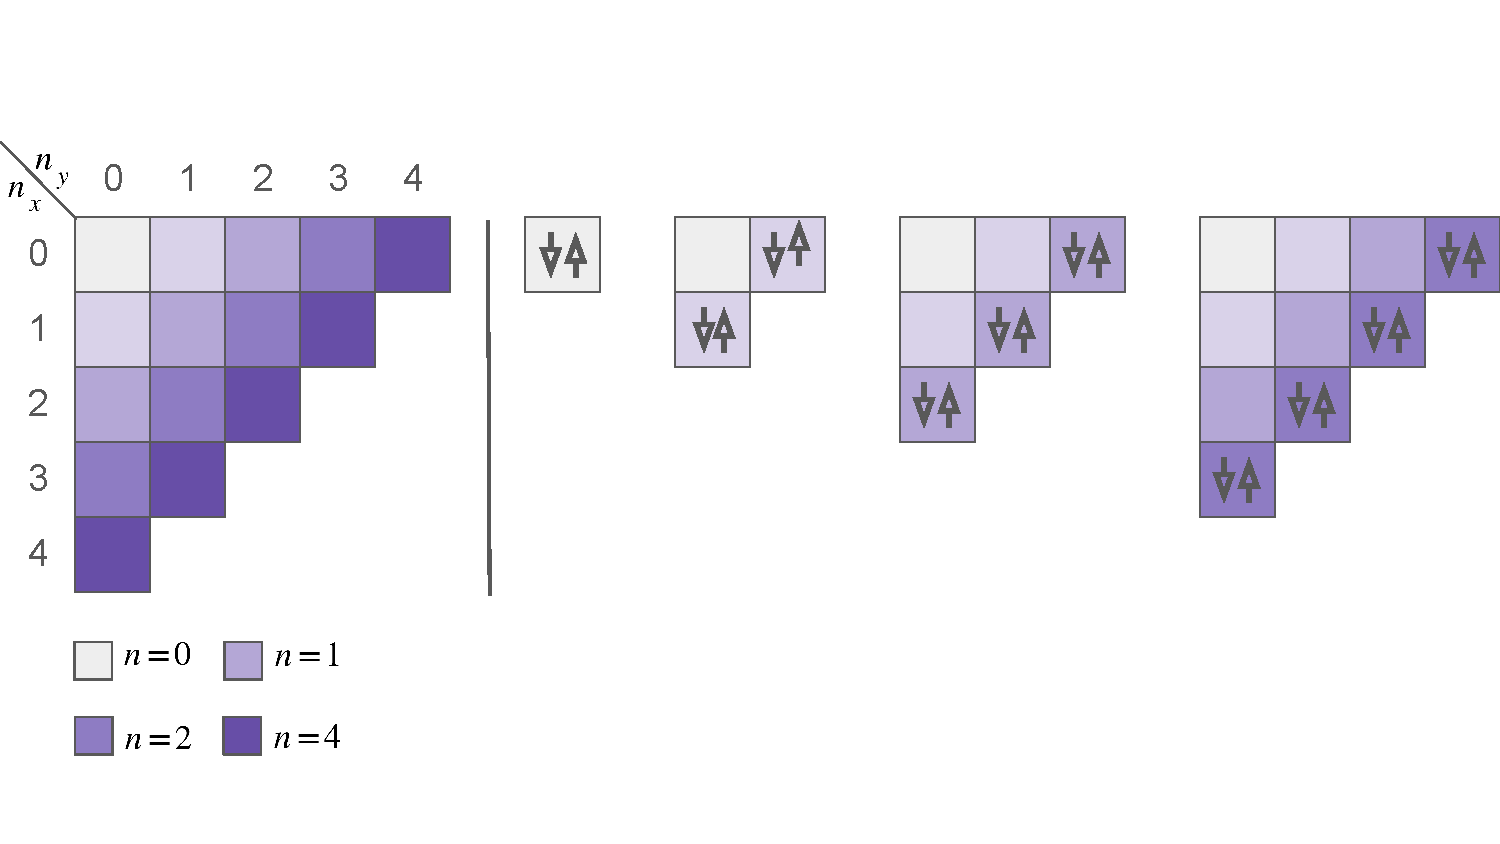
\includegraphics[width=0.8\linewidth]{Chapters/Theoretical_Background/images/energy-levels.pdf}
    \caption{Illustration of the possible $n_x$ and $n_y$ configurations in order to yield a specific principal number $n$ which determines the final energy level. Note that to obtain the number of electrons in the closed shell system one needs to fill the shell configurations \textbf{up to} the desired principal number.}
    \label{fig:energy_levels_2d}
\end{figure}

\subsubsection{Kato's Cusp Conditions}\label{sec:kato}
The Hamiltonian of a quantum mechanical system, as described by \eqref{eq:2body_hamiltonian}, can include an interaction potential that may exhibit singularities. The Coulomb potential, for example, follows an inverse proportionality to the distance between particles, expressed as $1/r_{ij}$, which diverges when the particles are arbitrarily close and $r_{ij} \to 0$.

To ensure that physical quantities such as the energy remain well defined, the singularity must be somehow offset by the kinetic term in the Hamiltonian. The fact that the kinetic energy of the system is merely proportional to the Laplacian of the wavefunction implies that the wavefunction itself must adhere to some mathematical conditions to counterbalance the singularity in the potential.

Kato's theorem, first presented in \cite{kato1957eigenfunctions}, provides a formal framework for the description of the wave function at those interaction singularity points. More specifically, it states that $\Psi$ must follow
\begin{align*}
    \left.\frac{\partial \Psi}{\partial r_{ij}} \right|_{r_{ij}=0} = \frac{m_i m_j}{m_i + m_j}Z_i Z_j \Psi(r_{ij} = 0),
\end{align*}
where $Z$ represents charge, and $m$ the masses of particles. As a consequence, a wave function following such a condition must have a cusp profile, or sharpness in the particle density at the singularities. The gradient of the wave function changes abruptly at $r_{ij} = 0$ in a way that controls the divergent potential.

As will be shown in \secref{sec:ansatz_closer_view}, this condition will guide our choice of a wave function in the computational implementation. Then we will require the use of additional terms for the ansatz, such as the Jastrow factor and the Padé-Jastrow factor.

%\subsection{Bosonic system}
%\subsubsection{Three-dimensional Bose-Einstein condensate}

%We now move to the discussion of a bosonic system of particular experimental importance. Similarly to the previous systems, the particles are also trapped in an HO potential. If we further assume the system to be at very cold temperatures, or even 0 Kelvin for our approximations, the trapped bosons tend to form what is known as a Bose-Einstein condensate, where all bosons accumulate at the lowest-energy state with the same quantum numbers.

%Because of this accumulation, the particles tend to be as statistically close as possible, being repelled only by their Coulomb interaction. This is especially challenging for computational simulations, as the Coulomb potential presents a singularity when $r_{ij} \to 0$. One way to counter that is to use an informed ansatz that satisfies Kato's cust conditions, as described in \secref{sec:kato}. Moreover, the interaction between two bodies was modelled using hard spheres, ensuring that the wave functions do not overlap.

%We then set a constant $a$ as the boson's hard-core diameter and an infinite repulsive potential should two particles $i$ and $j$ be separated by a distance less than $a$. When the separation exceeds $a$, the bosons are only influenced by the external potential. Represented as a piecewise function, the interaction is given by 
%\begin{equation}
% V_{int}(\mathbf{r}_i,\mathbf{r}_j) =  \Bigg\{
% \begin{array}{ll}
%	 \infty & {|\mathbf{r}_i-\mathbf{r}_j|} \leq {a}\\
%	 0 & {|\mathbf{r}_i-\mathbf{r}_j|} > {a}.
% \end{array}
%\label{eq:potential_int}
%\end{equation}

%As we already know at this point, studying the associated non-interactive problem can be useful for better understanding the physics and for numerical validation. The symmetry of the problem indicates that we can simply sum the respective energies for each dimension, which are the energies for the quantum harmonic oscillator, $E_{n_d} = \left(\frac{1}{2} + n_d\right)\omega$, where $d$ is simply a dimension index.

%In this bosonic case, given all particles are allowed to have the same quantum number and that the Hamiltonian is once again spin-independent, the energy of the ground-state system, for each dimension is simply the sum of the energy of individual particles in a quantum HO trap in the ground-state, 
%\begin{align}
%    E_{gs} = \frac{1}{2}ND\omega,
%    \label{eq:met:NIC_HO_gs_analytical}
%\end{align}
%with the noninteractive eigenfunction given by
%\begin{equation}
% \Psi_+(\mvec{r}_1, \mvec{r}_2, \ldots, \mvec{r}_N) 
%= C\left[\prod^N_i \exp\left(-\frac{r_i^2}{2}\right)\right],
%\label{eq:trialwf}
%\end{equation}
%with $C$ a normalisation factor.

\section{Classical and Quantum Correlations}

When discussing Monte Carlo simulations \secref{sec:VMC}, we will talk about correlations, although in a different sense.

Statistically, there are multiple ways to measure how random variables depend on or influence each other. This dependency is what we understand by correlation. Consider two random variables $A$ and $B$. The fact that those depend on each other can be expressed by the inequality 
\begin{align*}
P(A,B) \neq P(A)P(B).
\end{align*}

There exist correlation coefficients to measure how strongly this inequality holds, such as the Pearson correlation \cite{sedgwick2012pearson}. To make things explicit, there are at least three types of correlation that we would like to distinguish. First, if we allow the particles to interact, for instance, due to Coulomb interaction, observables such as position of one particle influence the probability density function of the others, inducing correlation.


Second, even if identical quantum particles do not interact classically, we know that (anti-)symmetry constraints induce correlation between states. In general, we know that $ \psi_{\alpha,\beta}(x_1,x_2) \neq\psi_\alpha(x_1)\psi_\beta(x_2)$, and even if in this example $\psi(x)$ is not a probability function, the argument still holds.

Lastly, entanglement is perhaps the most explicit type of quantum correlation. Entangled particles often have their measurement completely determined by the measurement of the entangled particle. Of course, not all correlated states are entangled. A system could be a classical mixture of factorisable pure states, in which case the joint probability densities for measurements on these two subsystems are accurately described by the classical probability theory of correlated random variables. On the other hand, entangled states can be mixtures of broader, non-separable states.
\chapter{Computational Background}\label{ch:computational}

\begin{figure}[h]
    \centering
    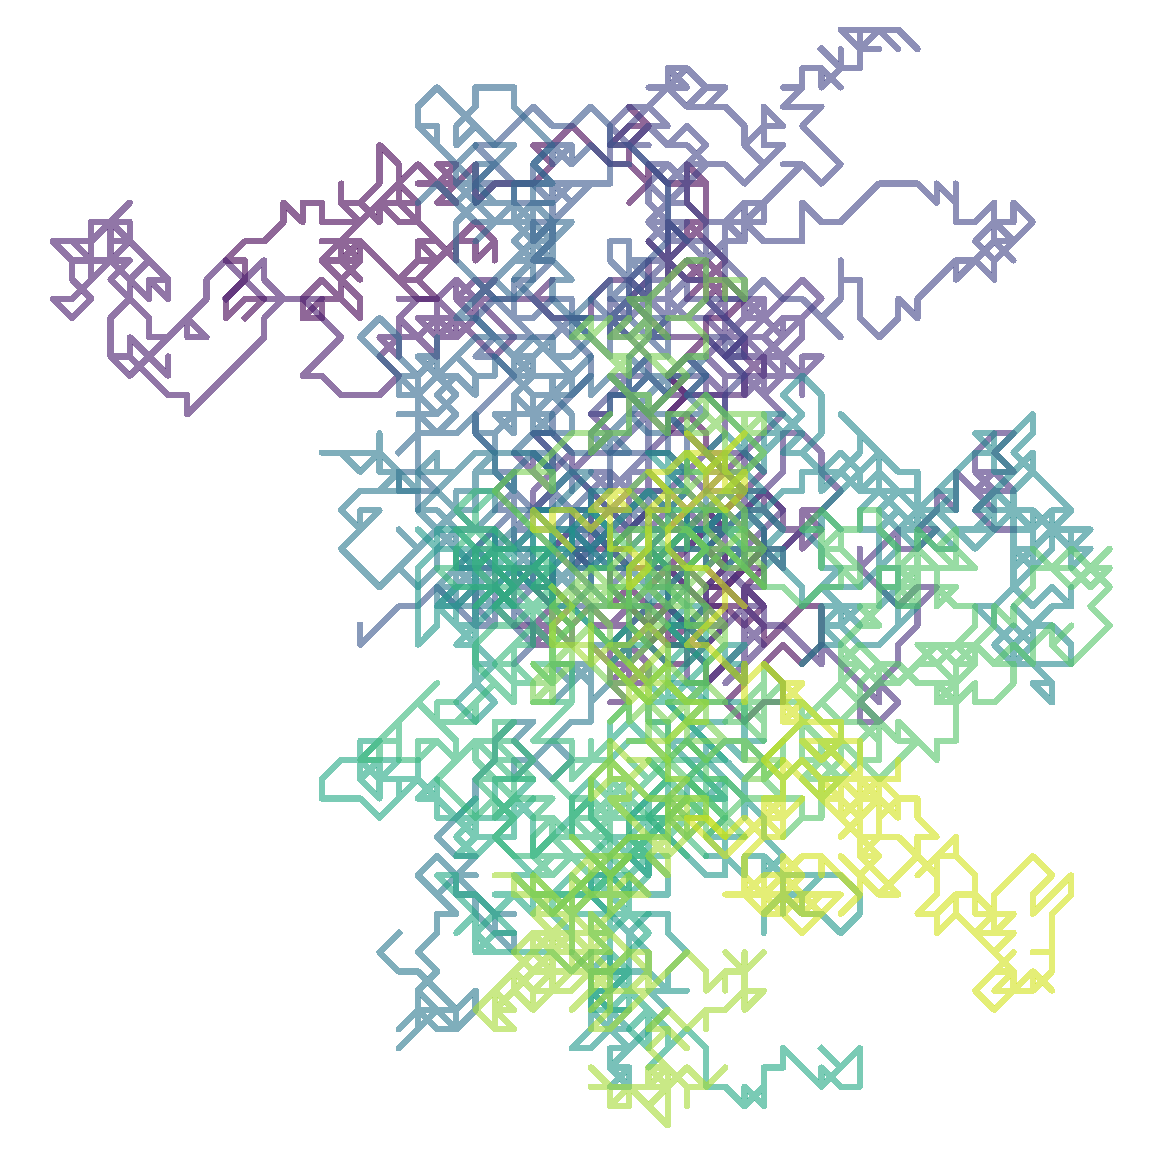
\includegraphics[width=0.8\linewidth]{Chapters/Theoretical_Background/images/random_walkers.pdf}
    \caption{Trajectory of 15 random walkers on a lattice, inspired by \cite{Nordhagen2019}.}
    \label{fig:walkers}
\end{figure}


\section{Sampling and Markov Chains}\label{sec:markov_chains}

Suppose that we wish to study a phenomenon in nature that is inherently stochastic and for which we lack prior information about its probability distribution. Then, collecting information from one single experiment is not significant. If we want to infer statistics from a set of events, we rely on sampling.

By sampling, we mean selecting a subset of a population from which to collect information. Doing so with specific statistics techniques allows us to infer information from the whole population without measuring every instance and with a good notion of how wrong the inferred values are. To eliminate unwanted bias in this collection process, it is common to conduct sample selection with some level of randomness.

In this discussion, random or stochastic variables will be denoted as $X$ and represent a function that maps a set of outcomes $\Omega=\{\text{outcome A}, \text{outcome B}\}$ to a set of numbers, for example $\{23, \pi\}$. To quote A. Eagle (2014) \cite{chancevrandomness}, one sees that a random variable is ``... neither random nor a variable''.

In the context of random variables, we will represent $P$ as the probability measure, defined in the sample space, while $p$ is its probability density function. Furthermore, we represent a conditional probability as $P(X=x | Y=y)$, that is, a probability of random variable assuming definite value $x$ given the knowledge that $Y$ has been evaluated $y$.

\subsubsection{Markov Chains}

A family of random variables indexed with a sequential notion $\{X_i\}$ is called a stochastic process. While this indexing could be discrete or continuous, in computer simulations we will work with discrete-time Markov chains. Furthermore, we disclaim that this section will compromise mathematical rigour in favour of a short and intuitive presentation of Markov chains. Therefore, some concepts such as irreducibility, ergodicity, and detailed balance will sometimes be used interchangeably.

A Markov chain is a specific type of stochastic process in which the notion of the future outcome is dependent only on the outcome of the current step, and not on the previous ones. More specifically, if the outcome of a random variable of the stochastic process is $X_{i^*} = x$, the outcome of $X_{i^* + 1}$ depends only on the value $x$, and not on any other $\{X_{j}\}_{j < i^*}$.

The way in which the Markov chain evolves is modelled
by the likelihood of a transition between two states, $t(x, y)$, where $x$ and $y$ belong to $S$, the space of all the outcomes of the stochastic variables. To correctly specify a Markov chain, we need an initial probability distribution $\pi_0$ at initial state, and the transition probabilities of the following states, meaning 
\begin{align*}
    P(X_0 = x) &= \pi_0(x), \\
    P(X_{n+1} = x_{n+1} | X_n = x_n) &= t(x_n, x_{n+1}).
\end{align*}

Note that we did not need to specify the previous states of the chain in the conditional probability, as per the definition of Markov chains. Sampling from this chain can be done by first sampling $X_0$ according to $\pi_0$, and subsequently sampling $X_n$ following $t(X_{n-1}, \cdot)$. 

It is common to associate $t(x,y)$ to elements in a transition matrix, representing the probability transition $x \to y$  of one time step. In this case, it makes sense to see $p^m = P(X_{n+m} = y | X_n = x)$ as matrix $t$ being applied in succession. Furthermore, the probability distribution guiding the outcome of the random variable $X_n$ can be written
\begin{align*}
    P(X_n = x) \equiv \pi_n(x) = \pi_0 t^n.
\end{align*}

There are several conditions that must be satisfied for our process to be a relevant Markov chain. For example, fixed a state $x$, there must be transition altogether (even if to the same state), so
\begin{align*}
    \sum_{y \in S} t(x, y) = 1.
\end{align*}

Another subtle point is that, since we study these chains for long-time evolutions, we want stochastic processes with ``nice'' asymptotic behaviour. For that to be possible, some requirements must be satisfied. First, we do not care about chains that go to subsets of the state space and never return. That would cause the isolation of the chain in a way that leads to a divergence in statistical quantities. More specifically, we say we want to study irreducible chains: chains for which any state can be reached in some finite number of steps. 

Looking at the other extreme case, we also do not want to study periodic chains, for a similar problem of lack of convergence to a stationary distribution. These conditions are usually condensed into the requirement that the Markov chain satisfies a so-called detailed balance condition, formulated as follows: $\forall x, y \in S \times S$, 
\begin{align}
    \pi(x)t(x, y) = \pi(y)t(y, x).
    \label{eq:detailed_balance}
\end{align}

That means that when the distribution has reached a steady distribution, the proportion of transitions from state $x$ to $y$ is the same as from $y$ to $x$. Given detailed balance, we can invoke two convergence theorems for finite-state Markov chains. The first one, with respect to the convergence of the distributions, and the other one with respect to the expected values of functions of the random variables. Those are the expected values we seek to sample.

First, if we have $t(x,y)$ the transition matrix of irreducible, aperiodic finite state Markov chains, $\forall x,y \in S \times S$, any initial distribution $\pi_0$ will lead to $\pi_n$ which converges to a stationary $\pi$, and we write 
 \begin{align}
     \lim_{n \to \infty} t^{n}(x, y) = \pi(y).
     \label{eq:chain_convergence1}
 \end{align}

Furthermore, for that stationary $\pi$ and considering $f(x)$ any function on the state space, for any initial $\pi_0$ it follows
\begin{align}
 P\left(\lim_{n \to \infty} \frac{1}{n}\sum_{k=1}^n f(X_k) = \sum_x f(x)\pi(x)\right) = 1.
 \label{eq:chain_convergence2}
\end{align}

This means that the expected value of $f$, which depends on the random variable, when sampled towards infinity, will tend to ever better approximate the true expected value of $f$. This theorem is crucial for Markov chain Monte Carlo, and it leads us into the topic of Monte Carlo methods.


\section{Markov Chain Monte Carlo}

\subsubsection{Monte Carlo Methods}
Monte Carlo (MC) methods are a very broad class of computational methods that use sampling to generate numerical results. These methods are used in scenarios where traditional computational approaches are impractical, making it more feasible to tackle the problem by introducing randomness and depending on the law of large numbers for approximate solutions. First seen as a ``last resort'', MC is now considered a robust approach, present extensively in scientific computing \cite{whyMC}.

Monte Carlo methods can be used to solve both probabilistic and deterministic problems. A probabilistic example would be risk assessment simulations, while a deterministic example would be calculations of intractable integrals. We will use Monte Carlo methods in two very intertwined contexts: for the evaluation of high-dimensional integrals and for sampling quantities that follow complicated or unknown probability distributions via Markov chains.

This sampling process for Monte Carlo methods is stochastic and the information obtained about the data is an inferred probability distribution with an associated random error. Despite this randomness in the estimation, the uncertainty range can be arbitrarily reduced, given the sufficient computational time, as eluded to in \eqref{eq:chain_convergence1} and \eqref{eq:chain_convergence2}.
 
To demonstrate this, let us explore the approximation of an integral using Monte Carlo sampling. Suppose that we want to compute the integral of a function $f(\mvec{x})$, over $\Omega \subset \mathbb{R}^d$, which has volume V. The naive MC approach is to sample uniformly $n$ points, $x_i$ of $\Omega$ to compute the fraction of these samples that is evaluated below $f(\Omega)$. Of course, the probability of this happening must be proportional to the magnitude of $f(x_i)$ and, consequently, to the integral value. Mathematically, this approximation boils down to
\begin{align}
    \int_\Omega f(\mvec{x})\,d\mvec{x} \approx V \frac{1}{n}\sum_{i=1}^{n} f(\displaystyle \rvx_i).
    \label{eq:mc_integration}
\end{align}

\subsubsection{A comment on random number generation}
The generation of truly random numbers in computer programmes is not feasible. What we do instead is generate apparently uncorrelated numbers with deterministic algorithms called pseudo-random number generators (PRNGs). Given a known initial state determined by a number $X_0$ which we call a seed, the algorithm can replicate a whole sequence $X_n$ of apparently random numbers. There are a myriad of PRNGs, with significant differences in terms of randomness quality, speed, cycle, and other characteristics. 

For a true uniform random variable, the generated numbers should be completely uncorrelated, and, in PRNGs, we try to avoid correlations between generated numbers as much as possible. However, since their number generation is deterministic, some level of correlation is inevitable, even if subtle.

In computer simulations, where random numbers are generated millions of times, a fast algorithm is absolutely essential. For illustration, we mention a well-known and reasonably fast algorithm: the Linear Congruential Generator (LCG). An LCG is defined by the recurrence relation
\begin{align*}
    X_{n+1} = (aX_n + c) \mod m,
\end{align*}
where the choice of $m$, $a$, and $c$ determines the specific generator and how long of a sequence of pseudo-random numbers will be before starting to repeat. The length of such a sequence is called the cycle, and modern PRNGs have cycles of around $2^{128}$ numbers.

Although PRNGs typically generate numbers uniformly between 0 and 1, there are techniques to enable these generators to produce numbers following specific, well-known distributions, such as the Gaussian distribution. Among these methods are the reverse transform method, rejection sampling, and transformation techniques such as the Box-Muller method. Ideally, when one wants to generate random samples following a specific low-dimensional distribution, these methods are excellent choices. Unfortunately, in higher dimensions, these become extremely inefficient, motivating the search for other algorithms. To illustrate this, we briefly introduce the rejection sampling method. Although we do not explicitly use it, it is a perfect bridge between Monte Carlo integration and Markov chain Monte Carlo.

\subsubsection{Rejection Sampling and Curse of Dimensionality}

\begin{figure}[h]
    \centering
    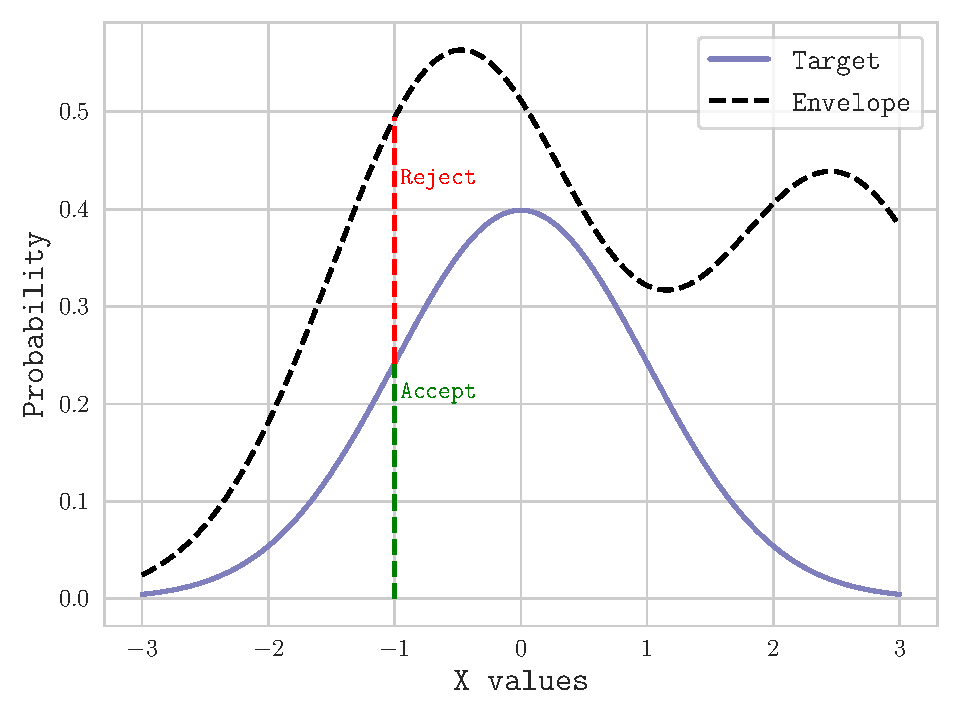
\includegraphics[width=0.6\linewidth]{Chapters/Theoretical_Background/images/rejection_sampling.pdf}
    \caption{Illustration of rejection sampling with an envelope and target distributions. Probabilities are not normalized.}
    \label{fig:rej}
\end{figure}

The idea of rejection sampling is to use a distribution from which we know how to sample, $g(x)$, to guide the sampling process and mimic the sampling of the distribution we desire, $p(x)$. This will work as long as $g$ is an envelope for $p$. More specifically, we need $p(x) < K g(x)$ for some scaling constant $K > 1$ and at any point in the function's domain. The iterative sampling process then follows three steps, which can be better understood with \figref{fig:rej}.
\begin{itemize}
    \item Sample a point $x$ from an envelope proposal distribution $g(x)$;
    \item Sample $y$ form the uniform $U(0, Kg(x))$;
    \item Accept and keep track only of samples for which $y < p(x)$.
\end{itemize}

With that, the normalised histogram that forms from the accepted samples tends to approximate the target distribution, indicating that the accepted samples indeed follow $p$. The problem with such a procedure, which is hard to see in low-dimensional examples, is that the rate of convergence for the approximation becomes slow in higher dimensions. The sampling is inefficient. In fact, the volume of rejected samples will increase at a much faster rate than that of the accepted ones, requiring a number of samples that is impractical. This is a consequence of the curse of dimensionality. 


\subsubsection{Markov Chain Monte Carlo}
To finally connect the concept of Monte Carlo integration with Markov chains, we can ask ourselves what would happen if, in \eqref{eq:mc_integration},  we sampled domain points using a general probability distribution $p$ instead of a uniform one. Recall that the expected value of a sample of $x$ following a probability distribution $p$ is denoted
\begin{align*}
    \E_{\rx\sim p}[f(X)] = \int f(x)p(x) dx,
\end{align*}
where we omit the domain for simplicity. If we compute the expected value of a function evaluated on domain points sampled following $p$ we solve a related but not exactly the same problem as the pure integral calculation of $f$. This expectation value can be approximated by the average of the samples,
\begin{align*}
    \E_{\rx\sim p}[f(\rx)] \approx \hat{\E}_{\rx\sim p}[f(\rx)] = \frac{1}{n}\sum_{i}^{n}f(x_i).
\end{align*}

As the number of samples $n$ increases, under the law of large numbers for Markov chains, this approximation will improve arbitrarily. Still, the question of how to generate samples from $p$ with Markov chains remains. As discussed in \secref{sec:markov_chains}, we require a Markov chain for which the stationary distribution is the one we want to sample from. In fact, there are different possible ways to do that, with maybe the two most common being the Metropolis and Gibbs algorithms. 

\subsection{Metropolis Algorithm }\label{sec:metropolis}

\begin{figure}[h]
    \centering
    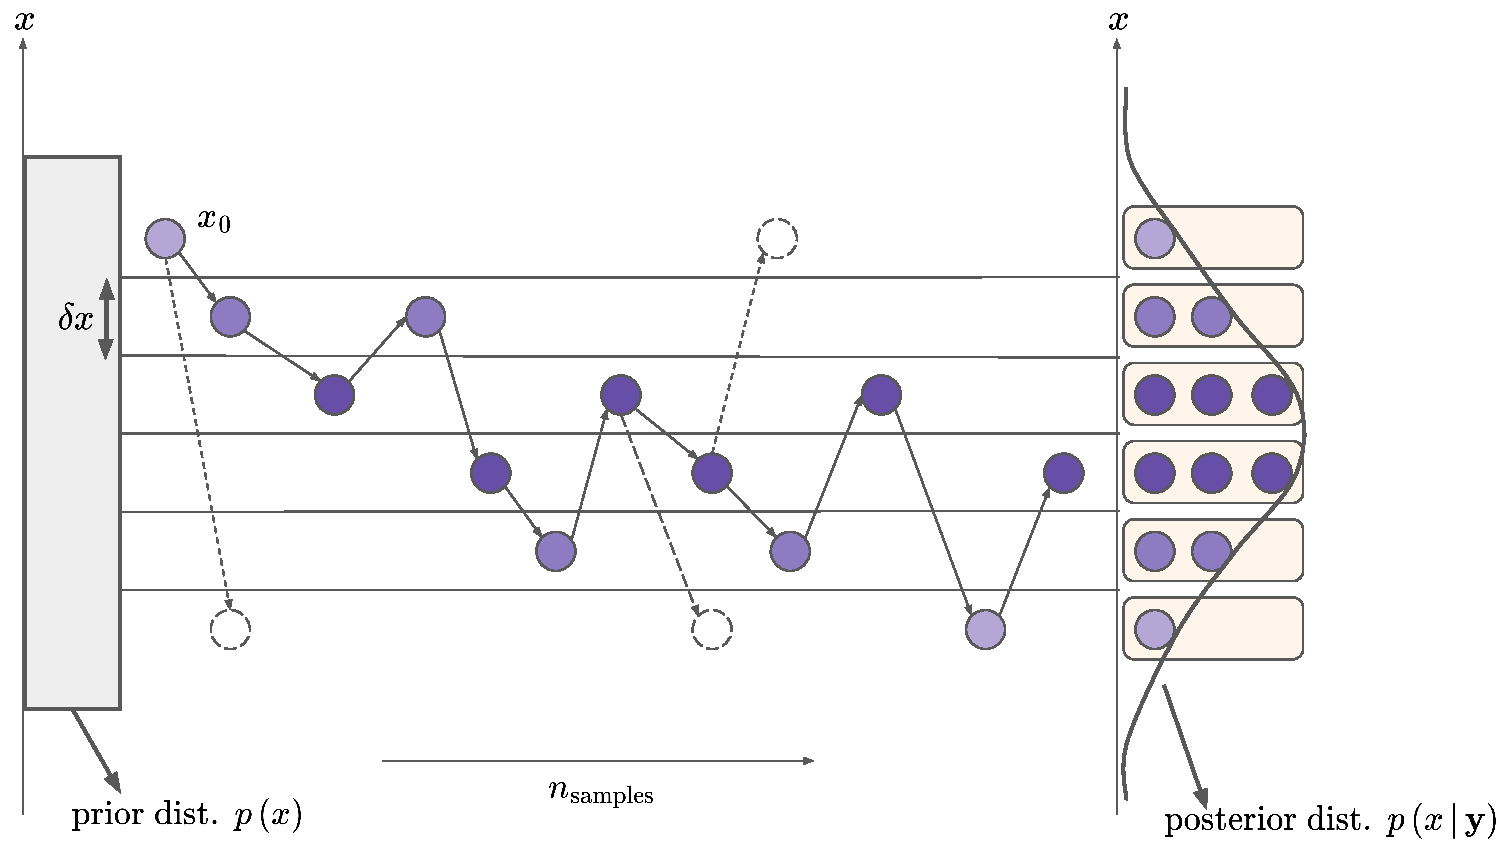
\includegraphics[width=0.8\linewidth]{Chapters/Theoretical_Background/images/metropolis.pdf}
    \caption{Illustration of using a prior distribution sampling to obtain samples from a posterior distribution by accepting and rejecting moves from an initial position $x_0$. Adapted from Lee et al., 2015 \cite{lee2015metamodel}}
    \label{fig:sampling_metropolis}
\end{figure}

Initially described in \cite{metropolisEquationStateCalculations1953}, the Metropolis algorithm serves as one method to generate a Markov chain to sample from, aiming to achieve a steady distribution that matches the target distribution. So far, we have not addressed how to get the correct transition probabilities $t(x, y)$ required from \eqref{eq:chain_convergence1}. The idea of Metropolis algorithm is to model a transition in state space via two independent probabilities. First, the transition state $y$ must be available, modelled by a proposal distribution $g(x,y)$. Moreover, there is a probability that $y$ is accepted $a(x,y)$ from the current state $x$. The fact that these are assumed independent means we can rewrite the detailed balance condition of \eqref{eq:detailed_balance} as
\begin{align*}
    \pi(x)a(x, y)g(x,y) = \pi(y)a(y, x)g(y,x),
\end{align*}
or, rearanging, 
\begin{align}
    \frac{a(x, y)}{a(y, x)} = \frac{\pi(y)}{\pi(x)}\frac{g(y,x)}{g(x,y)}.
    \label{eq:metropolis-hastrings-acceptance1}
\end{align}

Note that $g$ is something that we control and could be, for example, a normal distribution centred around the current state. Furthermore, it plays a similar role to the envelope distribution in rejection sampling. Satisfying \eqref{eq:metropolis-hastrings-acceptance1} above is equivalent to having an acceptance rule of
\begin{align}
    a(x, y) = \min\left(1, \frac{\pi(y)}{\pi(x)}\frac{g(y,x)}{g(x,y)}\right).
    \label{eq:metropolis-hastrings-acceptance2}
\end{align}

In other words, if we use such an acceptance rule with a proposal distribution that we control, we are still satisfying detailed balance. In this case, the sampled values will converge to the sampled values under the desired stationary probabilities. If we use a symmetric proposal distribution $g$ such as a normal distribution, \eqref{eq:metropolis-hastrings-acceptance2} further simplifies, given that the fraction of proposed probabilities will be one. Under this simplification, the Metropolis–Hastings algorithm is simply called Metropolis, but more often than not the names are used interchangeably.

A final comment on the Metropolis-Hastings algorithm is that, due to the fraction between $\pi(y)$ and $\pi(x)$, it allows us to sample quantities from $\pi(y)$ with any proportional probability distribution $f(x) \propto \pi(x)$. 

\secref{sec:VMC} includes an algorithmic recipe with algorithm box \ref{algo:general_update_rule}, although fitted to our variational Monte Carlo framework. In addition, \figref{fig:sampling_metropolis} illustrates the general idea of proposing steps from an initial state $x_0$ and accepting or rejecting them to generate a posterior distribution. 

\begin{JTD}
This last comment about allowing for a function $f \propto \pi$ can seem irrelevant but allows us to sample from distributions for which we lack knowledge of partition functions. In our case, it allows us to use an unnormalized ansatz in variational Monte Carlo. 
\end{JTD}

\section{Variational Monte Carlo}\label{sec:VMC}
As discussed in \secref{sec:choice_of_systems}, we are deeply interested in solving the Hamiltonian eigenvalue problem. More specifically, we are focused on the smallest eigenvalue and its eigenstate. We now see a way to approach this problem via Markov chain Monte Carlo, avoiding explicitly solving the Schrödinger equation.

By the variational principle, discussed in \secref{sec:var_principle}, any trial wave function yields and expectation value for the energy that is bounded from below by the true ground-state energy of the system. With that in mind, variational Monte Carlo (VMC) is a method that iteratively samples energy values from a parameterised trial wave function $\ket{\Psi_T(\mvec{\theta}) }$ and updates its parameters $\mvec{\theta}$ to drive the sampled energies to a minimum. VMC is heavily biased by the functional choice for the trial function, and finding a good initial guess can be extremely difficult. It is therefore an approximate method with potentially large error bars. 

Despite these challenges, VMC remains easy to implement in comparison to other more precise methods, such as diffusion Monte Carlo, while also avoiding the infamous sign problem \cite{Pan_2024}. The idea behind VMC is to note that, by using a trial wave function $\Psi_T$, one can express the expected value for any observable $O$ on a complete basis $\{\ket{\mvec{\alpha}}\}$ as 
\begin{align}
    \frac{\langle\Psi_T |\hat{O}|\Psi_T\rangle}{\langle\Psi_T |\Psi_T\rangle} &= \sum_{\mvec{\alpha}, \mvec{\beta}}\frac{\langle\Psi_T |\mvec{\alpha}\rangle\langle \mvec{\alpha} | \hat{O}|\mvec{\beta}\rangle \langle \mvec{\beta} |\Psi_T\rangle}{\langle\Psi_T |\Psi_T\rangle}\\
    &=\sum_{\mvec{\alpha}} \frac{\langle\Psi_T |\mvec{\alpha}\rangle\langle \mvec{\alpha} |\Psi_T\rangle}{\langle\Psi_T |\Psi_T\rangle}\sum_{\mvec{\beta}}  \langle \mvec{\alpha} | \hat{O}|\mvec{\beta}\rangle  \frac{ \langle \mvec{\beta} |\Psi_T\rangle}{\langle\Psi_T |\mvec{\alpha} \rangle}\\
    &=\sum_{\mvec{\alpha}}P(\mvec{\alpha})\sum_{\mvec{\beta}}O_{L}(\mvec{\beta}).
    \label{eq:exp}
\end{align}

The first term in the summation represents the normalised probability of the state $P(\mvec{\alpha})$, while the second term can be interpreted as a local operator estimator $O_L$. This allows us to approximate the expectation value on the left-hand side of \eqref{eq:exp} as the average of sampled values of the observable associated with the local operator. To better illustrate this, let us express the trial wave function as $\Psi_{\mvec{\theta}}(\mathbf{R})$ and deal with the Hamiltonian operator. This representation indicates a wave function parameterised by $\mvec{\theta}$ with $\mathbf{R}$ a collective variable of all positions of a multi-particle system. In this case, the VMC energy follows
\begin{equation}
    E(\mvec{\theta}) = \frac{\langle \Psi_{\mvec{\theta}}(\mathbf{R}) | \hat{H} | \Psi_{\mvec{\theta}}(\mathbf{R}) \rangle}{\langle \Psi_{\mvec{\theta}}(\mathbf{R}) | \Psi_{\mvec{\theta}}(\mathbf{R}) \rangle} =  \int E_L(\mathbf{R}) p(\mathbf{R}, \mvec{\theta}) \, d\mathbf{R} = \langle E_L \rangle_{\mathbf{R} \sim p(\cdot, \mvec{\theta})},
    \label{eq:vmc_energy_integral}
\end{equation}
where we have introduced the concept of a local energy $E_L$,
\begin{equation}
    E_L = \frac{\hat{H} \Psi_{\mvec{\theta}}(\mathbf{R})}{\Psi_{\mvec{\theta}}(\mathbf{R})},
    \label{eq:local_energy}
\end{equation}
and the probability density function $p_{\mvec{\theta}}(\mathbf{R})$,
\begin{equation}
p_{\mvec{\theta}}(\mathbf{R}) = \frac{|\Psi_{\mvec{\theta}}(\mathbf{R})|^2}{\int |\Psi_{\mvec{\theta}}(\mathbf{R})|^2 \, d\mathbf{R}}.
\label{eq:probability_density}
\end{equation}



This allows us to use Markov chain Monte Carlo to approximate the high-dimensional integral in \eqref{eq:vmc_energy_integral}:
\begin{equation}
\int E_L(\mathbf{R}) p_{\mvec{\theta}}(\mathbf{R}) \, d\mathbf{R} \approx \frac{1}{n} \sum_{\mathbf{R} \in \mathbf{R}_n \sim p_{\mvec{\theta}}(\cdot)} E_L(\mathbf{R}), 
\label{eq:mc_integration2}
\end{equation}
where $n$ denotes the number of samples $\mathbf{R}_n$ in a Markov chain framework. To see why this approximation is necessary, let us disregard spin degrees of freedom and try to compute the integral
\begin{align*}
    \langle H \rangle = \frac{\int dR_1 dR_2 \ldots dR_N \psi^* H \psi }{\int dR_1 dR_2 \ldots dR_N \psi^* \psi}.
\end{align*}

As detailed in \cite{hjorth-jensen2021}, evaluating this integral via Gaussian quadrature with 10 particles and 10 mesh points for each degree of freedom would take around $10^{18}$ seconds, or ten billion years. This calculation considers $10^{30}$ floating point operations in three dimensions, assuming that the calculations are performed on an ideal computer, which is totally impractical.

For an illustration on how to proceed with the calculation of the local energy of \eqref{eq:local_energy}, we can break down the Hamiltonian in terms of kinetic and potential energy. The potential term will depend on the system (external potential trap and particle particle interaction), but the local kinetic term can be written,
\begin{align*}
    \hat{K} = -\frac{1}{2}\frac{\mathbf{\nabla}^{2} \Psi_{\mvec{\theta}}}{\Psi_{\mvec{\theta}}}.
\end{align*}

For stability reasons, it is common, when dealing with VMC, to work with the wave function in the logarithmic domain \cite{sorellabook}. This approach helps especially with convergence stability, as the trial function can assume very small or very large values. The sign of the wavefunction must be kept, of course, if one wishes to retrieve the wavefunction expression and not just the probability distribution. In this case, the kinetic term follows
\begin{equation*}
    \hat{K} = -\frac{1}{2} \sum_{i=1}^N \left[ \left(\frac{\partial \ln\left|\Psi_{\mvec{\theta}}(\mathbf{R})\right|}{\partial R_i}\right)^2 + \frac{\partial^2 \ln\left|\Psi_{\mvec{\theta}}(\mathbf{R})\right|}{\partial R_i^2} \right],
\end{equation*} 
with $N$ the number of particles and $R_i$ refering to the vector coordinates of particle $i$. The derivation of this expression is available in Appendix \ref{appendix:vmc}.

The minimisation of the expectation value for the local energy can be achieved using a gradient descent optimisation approach, which will be further detailed in \secref{sec:Gradient-based optimisation}. In its simplest form, the iterative update of parameters can be represented as
\begin{equation}
    \theta_{(t+1)} = \mvec{\theta}_{(t)} - \nabla_{\mvec{\theta}} E(\mvec{\theta}),
\end{equation}
with $t$ the iteration index. A caveat here is that we are taking a derivative of the expectation value, which follows, dropping the $T$ subscript for simplicity:
\begin{align*}
    \nabla_{\mvec{\theta}} E(\mvec{\theta})= 
\frac{\int d\mathbf{R}\, (\nabla_{\mvec{\theta}}\Psi^*) H \Psi + \Psi^* H(\nabla_{\mvec{\theta}}\Psi)}{\int d\mathbf{R}\, \Psi^* \Psi }
- \frac{\left(\int d\mathbf{R}\, \Psi^* H \Psi\right) \nabla_{\mvec{\theta}} \left(\int d\mathbf{R}\, \Psi^* \Psi \right)}{\left(\int d\mathbf{R}\, \Psi^* \Psi \right)^2}.\\
\end{align*}
If we let $\mathcal{N} = \int d\mathbf{R}\, \Psi^* \Psi $ for simplicity and considering the wavefunction assumes only real values, it follows
\begin{align*}
    \nabla_{\mvec{\theta}} \mathcal{N} = 2 \int d\mathbf{R}\, \Psi \nabla_{\mvec{\theta}}\Psi 
\end{align*}
and
\begin{align*}
\nabla_{\mvec{\theta}} E(\mvec{\theta}) &= \int \frac{d\mathbf{R}\, (\nabla_{\mvec{\theta}}\Psi) H \Psi + \Psi H(\nabla_{\mvec{\theta}}\Psi)}{\mathcal{N} }
- 2\left\langle E_L\right\rangle\left\langle\Psi^{-1}\nabla_{\mvec{\theta}}\Psi\right\rangle\\
&=2\left(\left\langle E_L \cdot\Psi^{-1}\nabla_{\mvec{\theta}}\Psi\right\rangle-\left\langle E_L\right\rangle\left\langle\Psi^{-1}\nabla_{\mvec{\theta}}\Psi\right\rangle\right),\\
\end{align*}
which is also equivalent to, and more often seen as 
\begin{equation}
    \nabla_{\mvec{\theta}} E(\mvec{\theta})=2 \mathbb{E}_{\mathbf{R}\sim |\Psi_{\mvec{\theta}}|^2}\left[ \left(E_L
- E(\mvec{\theta})\right)\nabla_{\mvec{\theta}}\log \left|\Psi_{\mvec{\theta}} (\mathbf{R})\right|\right].
\label{eq:grad_el_vmc2}
\end{equation}

The real-valued wave function assumption in this derivation is reasonable in sight of our computational implementation: We will be dealing only with stationary states and bounded systems.

\subsection{Metropolis Algorithm and VMC}

With this rewriting, we move the difficulty of the problem from a high-dimensional integral to sampling from a distribution over the position space $\mathbb{R}^{Nd}$, where $N$ is the number of particles and $d$ the number of dimensions of the system. Then, a sequential Monte Carlo Markov chain proposal of steps is denoted $\Vec{R}^{(i)} \to \Vec{R}^{(i+1)}$ so that it depends only on the previous state at position $\Vec{R}^{(i)}$. Whether the new point $\Vec{R}^{(i+1)}$ should be accepted is evaluated according to an acceptance rule, such as \eqref{eq:metropolis-hastrings-acceptance2} for the Metropolis scheme. 

Given that $\Vec{R}^{(i+1)}$ represents the coordinates of all particles,  we propose new positions by moving either all particles at the same time or one at a time. Both Metropolis and the (to be discussed) Langevin Metropolis-Hastings require some proposal rule, which we write as $\mvec{\mu} = \mvec{\mu}(\mvec{\sigma}_1, \mvec{\tau}_1) \in \mathbb{R}^d$, where $\mvec{\sigma}_1$ are system-dependent parameters (such as $\Vec{R}, \Psi_T(\Vec{R})$) and $\mvec{\tau}_1$ are method-specific parameters. In addition, we define a metric $\nu = \nu(\mvec{\sigma}_2, \mvec{\tau}_2)$ used in the evaluation for the acceptance or rejection of the proposed points.

In the Metropolis algorithm, $\nu$ is compared to a random number drawn from a continuous uniform distribution $r \sim U_c(0,1)$. Should $\nu$ be larger than this number, the step is accepted. Otherwise, the configuration $\Vec{R}$ remains the same. There is also a need to initialise the particle positions, which greatly affects the convergence of the sampling. We will note this by the function $\mvec{\lambda}$, based on drawing positions following a probability distribution. In case we choose to move one particle at a time, the general movement of $\mvec{R}$ in the state space $\mathcal{S}$ can be seen in Algorithm \ref{algo:general_update_rule}. To better see how this extends in the whole context of variational parameter training, we refer to the Algorithm \ref{algo:nqs_update_rule}.
\begin{algorithm}[H]
    \begin{algorithmic}
            \STATE Initialize all particle positions $\Vec{R}^{(1)} \leftarrow \mvec{\lambda}$        
            \FOR{$i = 1, 2, \ldots, n$}
                \STATE Draw a random particle index $p \sim U_d[1,N]$ 
                \STATE Calculate new particle position $\Vec{R}'_p \leftarrow \Vec{R}^{(i)}_p + \mvec{\mu}$
                \STATE Calculate metric $w \leftarrow \nu(\Vec{R}', \Vec{R}^{(i)})$  %Assign I to I + f(x)
                \STATE Draw uniform number $r \sim U_c(0,1) $ 
                \IF{ $w \geq r $ }
                    \STATE Accept new position: $\Vec{R}^{(i+1)}_p \leftarrow \Vec{R}^{(i)}_p$ 
                \ENDIF
            \ENDFOR
    \end{algorithmic}
    \caption{Procedure to determine $n$ configurations in $\mathcal{S}$. $U_c$ and $U_d$ are continuous and discrete uniform probability distributions respectively. Here, we move one particle at a time.}
    \label{algo:general_update_rule}
\end{algorithm}

In the Metropolis algorithm, the normalisation constant of the probability density function in \eqref{eq:probability_density} will cancel when calculating the acceptance rule. More specifically, for the trial wave function of the quantum mechanical system of interest, the ratio of the trial step $\Vec{R} \to \Vec{R}'$ follows
\begin{align}
    \nu_{M}(\Vec{R}, \Vec{R}') = \frac{p(\Vec{R}')}{p(\Vec{R})} = \frac{|\Psi_T (\Vec{R}')|^2}{|\Psi_T(\Vec{R})|^2},
    \label{eq:met:metric_metropolis}
\end{align}
which leads to the acceptance rule 
\begin{align}
    a(\Vec{R}, \Vec{R}') &= \min\left(1, \nu_{M}(\Vec{R}, \Vec{R}')\right).
    \label{eq:acceptance_metro_def}
\end{align}

If a proposed step moves towards a higher probability density, $\nu_{M} > 1$, and we always accept the step. In addition, to adequately sample from the probability distribution, some steps towards lower density regions must also be accepted. To test whether this should be the case, we also compare $\nu_M$ with $r \sim U_c (0,1)$ (as can be seen in Algorithm \ref{algo:general_update_rule}). If each particle is allowed to move a step length of $\delta$ in each dimension for each iteration, using a continuous uniform distribution, the proposal rule can be written as
\begin{align}
    \mvec{\mu}(\delta) = \sum_{i=1}^{D} d_i \delta \hat{e}_{x_{i}}, \hspace{20px} d_i \sim U_c (-1, 1), \label{eq:met:update_rule_metropolis}
\end{align}
where $\hat{e}_{x_{i}}$ are single particle unit vectors. If $\delta$ is too small, only small changes of $\Vec{R}$ will be allowed between iterations, and the probability density ratio \eqref{eq:met:metric_metropolis} will often be close to one, in which case $\nu_{M} > r$ will be true for almost every step and almost every proposal will be accepted. Too high of an acceptance rate results in sample means that slowly converge to the population mean. On the other hand, if $\delta$ is too large, the proposed step $\Vec{R}'$ is likely to land in a low-density region of $p$, with most steps being rejected, little movement in $\mathcal{S}$ and many repeated samples. 

Hence, it is crucial to identify a value of $\delta$ that ensures a balanced ratio of accepted to rejected steps. This proportion, commonly known as the acceptance rate $A_r$, is generally associated with reliable results when it is approximately $0.5$ \cite{gelmanWeakConvergenceOptimal1997}.

The steps proposed by the Metropolis algorithm are in some sense naive since the proposal step $\Vec{R}'$ uses no information on the probability distribution, but only on the probability at individual points by evaluating $\nu_M$. This, once more, can lead to inefficient sampling in high-dimensional spaces and motivates the Langevin Metropolis importance sampling, to be introduced in \secref{sec:langevin_imporance}.

\section{Diffusion Monte Carlo}

Diffusion Monte Carlo (DMC) is a well-established method for employing Monte Carlo sampling and diffusion theory to computationally determine the ground-state energies in quantum systems. Although we do not use the method directly, we discuss it for two reasons. First, it is recognised for providing potentially exact results, which we use to benchmark our calculations. Moreover, DMC has been shown to require an importance sampling approach to the Metropolis algorithm \cite{kalos1974helium}. This approach, which guides the sampling distribution of the proposal steps, is also used by us in our VMC calculations. Our DMC discussion is conceptual, and a more in-depth treatment can be found in \cite{Apaja2018qmc, kosztin1996introduction}

The DMC method is motivated by looking at the time-dependent Schrödinger equation of \eqref{eq:sol_tdse} under imaginary time evolution. This means that we replace $it \to \tau$, and the solution described on an enumerable eigenbasis $\ket{\phi_i}$, ordered according to the ascending order of eigenvalues can be written
\begin{align*}
\ket{\Psi(\tau)} &= e^{-\hat{H}\tau}\ket{\Psi(0)} \\
                &= \sum_i e^{-E_i\tau} c_i\ket{\phi_i} = c_0e^{-E_0\tau}\left[\sum_i \frac{c_i}{c_0}e^{-(E_i - E_0)\tau}\ket{\phi_i}\right].
\end{align*}

This can be understood as an operator $\exp({-\hat{H}\tau})$ that acts so that other states decay exponentially to the ground-state. The closer $E_i$ is to $E_0$, the slower the decay rate. In practice, this time evolution is often unstable, and it is standard to shift the energy scale towards a trial value $E_T$, for example the energy of the non-interacting ground-state problem. Then, in the limit of long time evolution, the excited parts of the general state get projected to the ground-state, either by decaying, if $E_i - E_T > 0 $ or by amplification, in case $E_L- E_T < 0$:
\begin{align*}
\ket{\Psi(\tau \to \infty)} \to c_0 e^{-E_0\tau} \ket{\phi_0}.    
\end{align*}

Under this lens, DMC models the evolution in imaginary time as a generalised diffusion process, where energy terms act as either sources or sinks. Initially conceptualised by E. Fermi in the 1940s, this scenario is described through random walkers experiencing birth-or-death processes. 

The operator responsible for the diffusion evolution, which is now shifted by $E_T$ is the Greens's function,
\begin{equation*}
    \hat{G}(\tau) = e^{-(\hat{H} - E_T)\tau}.
\end{equation*}

After appropriate basis transformations necessary for us to solve the problem computationally, it is possible to write the Green's function in such a representation that yields 
\begin{equation*}
    \Psi(\mathbf{R}, t + \tau) = \int G(\mathbf{R},\mathbf{R}',\tau) \Psi(\mathbf{R}', t + \tau) d\mathbf{R}'.
\end{equation*}

Furthermore, under what is called the short-time approximation for the Green's function, one is able to approximate $G$ as a product of a diffusion part, $G_d$, and a branching part $G_b$, with $G_d$ attributed to the kinectic energy and $G_b$ to the potential energy.
\begin{equation}
    G(\mathbf{R},\mathbf{R}',\tau) \approx G_d(\mathbf{R},\mathbf{R}',\tau)G_b(\mathbf{R},\mathbf{R}',\tau)
\end{equation}

We now provide a brief description of how the rest of a naive DMC algorithm would be carried out. For each iteration, the branching part $G_b$ is used to evaluate whether walkers should be created or destroyed from the sampling procedure. Then, the walkers positions are allowed to move following the diffusion due to $G_d$. The specifics of the branching process and subsequent data collection are not covered in this discussion. Nevertheless, we explore further the diffusion process as it provides inspiration for our VMC implementation.

The diffusion Green's function must satisfy the diffusion equation:
\begin{equation}
    \frac{\partial G_d(\mathbf{R},\mathbf{R}',\tau)}{\partial_\tau} = -D \nabla^2_\mathbf{R}G_d(\mathbf{R},\mathbf{R}',\tau),
\end{equation}
in which case the solution is 
\begin{equation}
    G_d(\mathbf{R}',\mathbf{R},\Delta t) = \frac{\exp{\left(-\frac{(\mathbf{R}'-\mathbf{R})^2}{4D\Delta t}\right)}}{(4\pi D\Delta t)^{3N/2}}, 
\end{equation}
with D a diffusion constant and $\Delta t$ a free parameter time step. In the quantum mechanical case, $D = \hbar^2/2m$ or, in natural units, simply $D = 1/2$. If no importance sampling algorithm is used, such distribution can be sampled by making walkers move similarly to standard metropolis algorithm with a proposal
\begin{align*}
    \mathbf{R}' = \mathbf{R} + \mvec{\eta}\sqrt{2D\Delta t},
\end{align*}
with $\mvec{\eta}$ such that for each particle, $\eta$ is a d-dimensional Gaussian. Then, the acceptance criteria follows
\begin{align*}
    a(\Vec{R}, \Vec{R}') &= \min\left(1, \frac{G(\mathbf{R}',\mathbf{R}, \Delta t)}{G(\mathbf{R}, \mathbf{R}', \Delta t)}\nu_M\right),
\end{align*}
with $\nu_M$ the metropolis metric. However, as already mentioned, DMC requires a more guided sampling process, which we introduce now. 

\subsection{Langevin Metropolis Importance Sampling}\label{sec:langevin_imporance}
Often in quantum-mechanical simulations, the probability distribution to be inferred from sampling can be somewhat localised. Then, a significant portion of the stochastic integration steps gets wasted in regions that are not representative of the target distribution. More critically, unguided Monte Carlo sampling leads DMC walkers towards regions of infinite potential and unstable results.

The Langevin Metropolis importance sampling method aims at guiding the acceptance probability to the target distribution of the trial wave function. This is done by introducing a quantum force or drift force, as explained in depth in \cite{chin1990langevinimportance}. Under the action of a drift force, $\mathbf{F}$, the evolution of a probability distribution $P(\mathbf{R}, t)$ can be modelled by the Fokker-Planck equation:
\begin{equation}
\frac{\partial P(\mathbf{R}, t)}{\partial t} = D\nabla\left[(\nabla - \mathbf{F}(\mathbf{R}))P(\mathbf{R}, t)\right].
\label{eq:fokker_plank}
\end{equation}
The relation between $\mathbf{F}$ and $P$ can be further investigated under some assumptions. It can be shown \cite{Fleisher2018} that since the force must act in the orthogonal direction of the diffusion, and given that in the stationary state, the left-hand side of \eqref{eq:fokker_plank} must be zero, the quantum force can be expressed as $\mathbf{F} = P^{-1}\nabla P$. In this case, for a particle $k$ at position $\mathbf{R}_k$,
\begin{equation*}
    \mathbf{F}(\mathbf{R}_k) = \frac{2\nabla\Psi(\mathbf{R}_k)}{\Psi(\mathbf{R}_k)}.
\end{equation*}

Invoking now the Langevin equation \cite{van1992stochastic}, which tells us how a stochastic variable can evolve under the time evolution of the distribution, a proposal $\mathbf{R}' = \mathbf{R} + \mvec{\mu} $ is given by 
\begin{align}
    \mvec{\mu}(\Vec{R}, \Delta t) &= D \mathbf{F}(\Vec{R})\Delta t +  \xi \sqrt{\Delta t} \label{eq:met:update_rule_metropolis_hastings},
\end{align}
with $\xi$ following a $d$-dimensional Gaussian distribution and $\Delta t$ follows the similar role as the step-length in regular Metropolis. The importance sampling algorithm then expresses the distribution $g$ in the acceptance rule of \eqref{eq:metropolis-hastrings-acceptance2} as the solution for the Fokker-Planck equation, which is the Green's function
\begin{equation}
    G_d(\mathbf{R}',\mathbf{R},\Delta t) = \frac{\exp{\left(-\frac{(\mathbf{R}'-\mathbf{R}-D\Delta t \mathbf{F}(\mathbf{R}))^2}{4D\Delta t}\right)}}{(4\pi D\Delta t)^{3N/2}}, \label{eq:met:metric_metropolis_hastings}
\end{equation}
which corresponds precisely to the diffusion component of the Green's function in the DMC context, $G_d$, now incorporating a drift term. If we are using a VMC algorithm instead of DMC, there is by definition no branching part of the general Green's function. In that case, we can express the modified acceptance criteria of this method as 
\begin{align}
    a(\Vec{R}, \Vec{R}') &= \min\left(1, \nu_{LMH}(\Vec{R}, \Vec{R}')\right), \notag\\
    \nu_{LMH}&=\frac{G_d(\mathbf{R}',\mathbf{R}, \Delta t)}{G_d(\mathbf{R}, \mathbf{R}', \Delta t)}\nu_M.
    \label{eq:acceptance_langevin_metro_def}
\end{align}

In words, the importance sampling guidance works by adjusting the acceptance probability such that the metric of \eqref{eq:met:metric_metropolis} is multiplied by the fraction of two Green's functions that model the transition probability between state $\mathbf{R}' \to \mathbf{R}$ of a probability distribution evolving due to a diffusion and a quantum force. In contrast to Metropolis, this algorithm adds, both in \eqref{eq:met:metric_metropolis_hastings} and \eqref{eq:met:update_rule_metropolis_hastings}, physical information about the trial wave function, indicating at least in theory a more robust method.

\subsubsection{A comment on DMC}

One of the advantages of DMC over VMC is that, in VMC, occasional excited states can contribute to the minimised energy via local minima, whereas in DMC calculations, excited states exponentially decay to the ground-state in the imaginary time evolution.

Despite being extremely precise, DMC also presents a couple of drawbacks. First, there is the constant problem of computational cost. For bosonic systems, DMC scales polynomially with the system size, but for fermionic systems, the scaling is exponential. Furthermore, and perhaps more important, is the fermionic sign problem: DMC can only be performed assuming wave functions that are positive at any evaluated point. Although techniques are used to circumvent this, such as the fixed node approximation \cite{anderson1975random}, they all bias the samples in some way.

\chapter{Machine Learning Background}\label{chap:ml}

\begin{figure}[h]
    \centering
    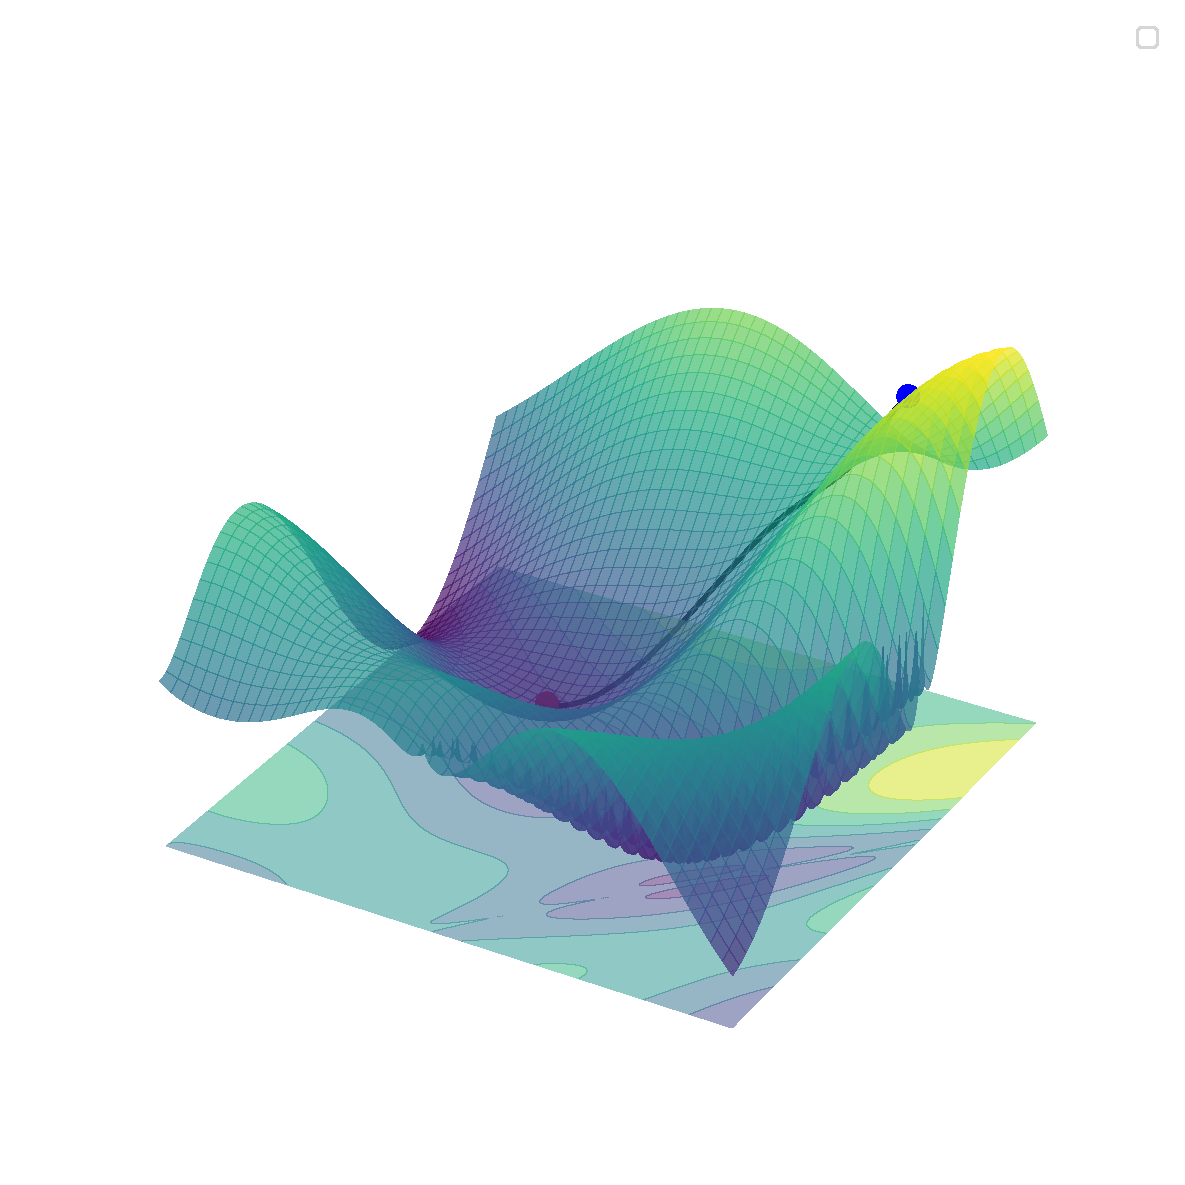
\includegraphics[width=0.8\linewidth]{Chapters/Theoretical_Background/images/eggholder.pdf}
    \caption{A gradient descent trajectory failing to optimise to global minima on the Eggholder function.}
    \label{fig:eggholder}
\end{figure}

The name machine learning, combined with its current overuse, can sometimes be misleading. Machine learning methods need no modern machines as we know them today. Given a pen, paper, and enough time, anyone can do machine learning. More precisely, what these methods do need is a computational machine - be it a human or a modern computer. Of course, the computer here would have an advantage in terms of automation and floating-point operations per second, and that is why we use them.

We will often refer to machine learning as statistical learning, as this name is more informative and helps to reduce some mysticism around the field.

\blindmathtrue
\section{Statistical Learning}

Statistical learning involves utilising statistics to extract knowledge from data. We therefore must clarify the meaning of data and learning in this context. First, there are various types of learning, typically categorised into supervised, unsupervised, and reinforcement learning. In supervised learning, the aim is to create a model that takes labelled examples as input and predicts outputs. The goal of unsupervised learning is to identify patterns or structures within the data, without explicit labels in the inputs. Lastly, reinforcement learning is distinct in that an agent makes decisions and interacts with an environment to obtain rewards based on its actions.

Consider a function $f :  X \to Y$, where $X$ is a set of possible inputs with $Y$ the set of all possible outputs. Here, data refers to subsets or sample vectors $x_i$ and $y_i$ from the respective sets, which makes $\{x_i, y_i\} \in X \times Y$. Learning, then, is the process of creating a model $\hat{f}(x_i)$ that model $f$ up to some error $\epsilon$,
\begin{align*}
    \hat{f}(x_i) = y_i + \epsilon_i.
\end{align*}

The error, or noise term, is a deviation of the model prediction from the actual output, and can occur from inherent fluctuations of the dataset or limitations of the model itself. In the case of an idealised model $\hat{f}$, we assume that $\epsilon$ follows a normal distribution $\mathcal{N}$, which is motivated by the law of large numbers.

Training a model involves searching for a model which minimises this error as much as possible. We are, however, free to choose how this error is measured, and, as we will discuss, that will greatly influence the minimisation search. For now, let us simply state that such a function, which represents a distance between the model's prediction and ground truth, should map to a real number. We will call it a loss function $\mathcal{L : \mathcal{H}} \to \mathbb{R}$, with $\mathcal{H}$ a set of all possible functions from input to output space\footnote{Note that this is not just any function, as the type of model adds constraints: it could be linear model, neural network, and so on.}. For now, we simply write
\begin{align}
    \mathcal{L}(f, \mathcal{D}) \propto \sum_{(x_i, y_i)\in \mathcal{D}}d(f(x_i), y_i),
    \label{eq:loss_as_average}
\end{align}
where $\mathcal{D} \subset X\times Y$, and $d$ a measure of the distance of the individual predictions to the truth. For now, it suffices to state that it will be a convex function such as the mean squared error.

\subsection{Learning as \MakeLowercase{a}n Optimisation Problem}\label{subsec:Learning as opt}

To quote Bennett \cite{bennett2006interplay}, ``Optimization problems lie at the heart of most machine learning approaches''. On that note, the objective of our learning is to find a function that, given a data set $\mathcal{D} = \{(x_i, y_i)\}$ from a hypotesis space $\mathcal{H}$, minimises $\mathcal{L}$. In mathematical terms, the problem becomes
\begin{align}
    \min_{f \in \mathcal{H}}\mathcal{L}(f, \mathcal{D}).
    \label{eq:min_prob}
\end{align}

However, this is only part of the problem. In statistical learning, we want models capable of generalising to unseen data. We want models to learn general features of datasets, rather than hyper-specialising on a specific one. This discussion is central to supervised learning and is deeply related to the concept of bias-variance trade-off, better discussed in \cite{hastie2009elements}. This specialisation process usually comes with an increase in complexity of the model, which leads to a higher variance, albeit smaller bias in the prediction values. To better estimate that, one usually breaks the data set into a training and testing set. Here we deliberately avoid that discussion as this technique is not used in our methods.

\section{Gradient-based Optimisation}\label{sec:Gradient-based optimisation}
There are several ways to approach optimisation problems, such as the one described in Section \ref{subsec:Learning as opt}. The technique of choice depends on the nature of the problem at hand, but perhaps the most famous is gradient-based optimisation. For a large class of problems, many functions we want to minimise - or maximise - are based on physically or statistically reasonable functions. For that reason, they are frequently well behaved in the differential calculus sense. If a specific loss function is sufficiently smooth\footnote{has well deffined derivatives up to some order $k$ over some domain $\mathcal{D}$. }, and has an extrema (minimum or maximum) at some point in the domain, we know $\nabla\mathcal{L} = 0$. 

Note how the domain of $\mathcal{L}$ is a very general vector space of functions. To make the differentiation process more intuitive, we parameterise a model $f_{\mvec{\theta}}: X \to Y$. This means that after fixing a functional form, we can explore the hypothesis space by changing the parameters $\mvec{\theta}$, and so the optimisation quest becomes
\begin{equation}
\mvec{\hat{\theta}} = \text{arg}\min_{\mvec{\theta}} \mathcal{L} (f_{\mvec{\theta}}, \mathcal{D}).
\label{eq:optimisation}
\end{equation}

\subsubsection{Steepest Descent}\label{sub:steepest}
The idea behind steepest descent (SD) is to iteratively update $\mvec{\theta}$ in a direction that minimises $\mathcal{L}$ and to do so using the gradient of the loss with respect to the parameters. The motivation is simple: this gradient should be related to the direction in which $\mathcal{L}$ decreases the most for the smallest displacement $\mvec{\delta}_{\theta} = \mvec{\theta}_{t+1} - \mvec{\theta}_{t}$. The word ``related'' carries a significant conceptual weight here, especially because we have not defined how to measure such displacement. For now, we shall use the Euclidean norm, in which case we write
\begin{equation*}
d\left(\mvec{\theta}_{t+1}\,,\,\mvec{\theta}_{t}\right)\,=\,\norm{ \mvec{\delta}_{\theta}}_2.
\label{eq:dist}
\end{equation*}

Our wordy motivation for steepest descent can then be written mathematically if we first take a first order approximation of $\mathcal{L}$ around $\mvec{\theta}_{t}$:
\begin{equation}
    \mathcal{L}(\mvec{\theta}) \approx \mathcal{L}(\mvec{\theta}_{t}) +  \mvec{\delta}_{\theta}^\top \nabla \mathcal{L}(\mvec{\theta}_{t}).
    \label{eq:taylor}
\end{equation}

Performing an iterative minimisation with the smallest possible step can be posed as a constraint minimisation problem. If we set the distance to an arbitrary but fixed scalar, $d\left(\mvec{\theta}_{t+1}\,,\,\mvec{\theta}_{t}\right)\,= \epsilon$, the quest for the optimal parameter can be written
\begin{align}
    \mvec{\theta}_{t+1}\,=\arg \min_{\mvec{\theta}}\left[\mathcal{L}(\mvec{\theta}_{t}) +  \mvec{\delta}_{\theta}^\top\nabla \mathcal{L}(\mvec{\theta}_{t})\,+\, \epsilon \right].
    \label{eq:steepst_argmin}
\end{align}

We have constrained the minimization of $\mathcal{L}$  to a function $d$, which can be solved via Lagrange multipliers (see Appendix \ref{appendix:steepest}), yielding
\begin{equation}
\mvec{\theta}_{t+1} = \mvec{\theta}_t - \alpha \nabla \mathcal{L}(\mvec{\theta}_t)    .
\label{eq:gradient_rule}
\end{equation}

The parameter $\alpha$, called the learning rate, is a scaling factor from the Euclidian distance, together with the displacement constraint $\epsilon$. In real-life applications, we often choose such a parameter experimentally. Using too big of a learning rate will mean that the constraint has not been satisfied, and steps are taken outside of the trust region which guarantees the linear approximation of the method.

Steepest descent has some pitfalls. First, all directions in parameter space are treated equally, in terms of scale, by the fixed learning rate. Depending on the parametrisation of our cost function, this might be a terrible assumption. Second, the learning rate is fixed; then, a large learning rate might make it impossible to reach convergence. Note that employing an extremely small learning rate is not practical either, as it would require more iterations to reach convergence and inevitably more computational time. Hereafter we will discuss some of the techniques to try and address these points. 

\subsubsection{Newton's Method}

The most immediate way to address the problem of equal treatment of the parameter scale is to use a higher-order Taylor expansion in \eqref{eq:taylor}. This is the essence of Newton's method. In this case, the update rule guided by the minimisation is expressed as 
\begin{equation}
\mvec{\theta}_{t+1} = \arg \min_{\mvec{\theta}} \left[\mathcal{L}(\mvec{\theta}_t) +  \mvec{\delta}_{\theta}^\top \nabla \mathcal{L}(\mvec{\theta}_t) + \frac{1}{2}  \mvec{\delta}_{\theta}^\top \text{H}(\mvec{\theta}_t)  \mvec{\delta}_{\theta} + \epsilon \right],
\label{eq:newtons_minimisation}
\end{equation}
for which the update rule becomes
\begin{align}
\mvec{\theta}_{t+1} &= \mvec{\theta}_t - \alpha \text{H}^{-1}(\mvec{\theta}_t)\nabla \mathcal{L}(\mvec{\theta}_t)\\  
\text{H}(\mvec{\theta}_t)&=\nabla^2 \mathcal{L}(\mvec{\theta}_t)
\label{eq:newtons_method}
\end{align}
where $\text{H}$ is the so-called Hessian matrix.

Newton's method improves the step towards the direction of the negative gradient of the loss function by adding information of the curvature of the objective function $\mathcal{L}$ via the Hessian matrix. While several of the theoretical arguments behind both SD and Newton's method are tailored to convergence in a convex landscape, they can be used in non-convex problems with some caution and techniques.

Convex functions are characterised by the property that the line segment connecting any two points on the function's graph always remains above the graph itself. A classical example being a parabola, optimisation on those functions is straightforward, as any local minima are also global minima. In contrast, non-convex functions do not have this guarantee, due to the potential presence of several local-minima or saddle points. In the latter class of functions, having bad initialisation points can in the worst scenario lead to divergence in the algorithm or lead to convergence to local minima. 

At this point, one might ask why not always use Newton's method. As for most computational problems, the answer is both storage and computational efficiency. The Hessian matrix is quadratic in number of parameters and has to be updated and stored for every iteration of the training process. Calculating the elements of the matrix is also expensive, since it involves the double derivatives of the objective function, and finally, inverting a matrix also has approximately cubic complexity. 

\subsubsection{Momentum Gradient Descent} 

The steepest descent method of Subsection \ref{sub:steepest} with update rule given by \eqref{eq:gradient_rule}, can be rewritten as
\begin{align*}
    \mvec{\delta}_t &= \alpha \nabla_{\mvec{\theta}} \mathcal{L}, \\
    \mvec{\theta}_{t+1} &= \mvec{\theta}_{t} - \mvec{\delta}_t .
\end{align*}

A simple improvement in this method is the addition of a moment term $\gamma \in (0,1)$. This parameter controls the maintenance of some information, or memory, about the convergence behaviour of the parameter update in previous epochs. The analogy arises as the moment of a particle increases, while its potential energy on a downward trajectory is minimised. The intuitive argument for this analogy is that, by having moment, such a particle traversing a landscape is able to overcome potential local minima or move ever so fast when in regions with a steady downhill trajectory. Following this reasoning, the algorithm follows
\begin{align*}
    \mvec{\delta}_t &= \gamma \mvec{\delta}_{t-1}  + \alpha\nabla_{\mvec{\theta}} \mathcal{L}, \\
    \mvec{\theta}_{t+1} &= \mvec{\theta}_{t} - \mvec{\delta}_t.
\end{align*}

This is an exponentially weighted average of displacements along the epochs, with the moment term $\gamma$ controlling how much to remember from the previous iterations. This constant is therefore a number between 0 and 1, to be fine-tuned experimentally. Note that this memory term invariably contains some information about the curvature of the landscape, while still being part of a first-order method.

\subsubsection{Root Mean Squared propagation (RMSprop)}

We have mentioned that a constant learning rate can affect the convergence of the training. We now present two examples among the class of adaptative learning rate methods that attempt to address this problem.

To avoid the computational cost of taking the second derivative of the loss function, RMSProp \cite{graves2013generating} aims at correlating this information with the moving average on the squared gradient of each parameter, represented here as $\mvec{s}_t$, and modulated by a decay rate $\beta$. This method assigns individual effective learning rates for each parameter and also modulates them by a decay rate. This makes the algorithm move fast in the beginning (large learning rate) when we are probably distant from the minima, and then proceed with caution as we hope to approach convergence:
\begin{align*}
    \mvec{s}_t &= \beta \mvec{s}_{t-1}  + (1- \beta)(\nabla_{\mvec{\theta}} \mathcal{L}\odot \nabla_{\mvec{\theta}} \mathcal{L}), \\
    \mvec{\theta}_{t+1} &= \mvec{\theta}_{t} -  \frac{\alpha}{\sqrt{\mvec{s}_t + \epsilon}} \odot \nabla_{\mvec{\theta}}\mathcal{L},
\end{align*}
where $\epsilon$ serves as a stability factor to avoid division by 0, and is usually a number around $10^{-9}$.

\subsubsection{Adaptative Moment Estimation (Adam)} 

Another widely used method that takes into account the second moment of that gradient is Adam or Adaptive Moment Estimation \cite{kingma2014adam}. In contrast to RMSProp, Adam considers both the first order ($\mvec{m}_t$) and the second order moment ($\mvec{s}_t$) of the gradient of each parameter, being a combination of momentum GD and RMSProp. Adam further includes bias corrections to these moments, denoted respectively $\mvec{\hat{m}}_t$ and $\mvec{\hat{s}}_t$. We will not derive the expression of these corrections, but the original authors of the paper argue for their motivation: since the first- and second-moment terms are exponentially weighted averages, their initialisation value of zero inevitably introduces a bias into their accumulation value. 

Adam has been shown to be an extremely robust optimisation algorithm, which means that it performs well in a wide class of different problems \cite{reyad2023modified, zhang2022adam}. For our use and purposes, we simply state the update rules below,
\begin{align*}
    \mvec{m}_t &= \beta_1 \mvec{s}_{t-1}  + (1- 
    \beta_1)\nabla_{\mvec{\theta}} \mathcal{L}, \\
    \mvec{\hat{m}}_t &=  \frac{\mvec{m}_t}{1- \beta_2^t}, \\
    \mvec{s}_t &= \beta_2 \mvec{s}_{t-1}  + (1- \beta_2)(\nabla_{\mvec{\theta}} \mathcal{L}\odot \nabla_{\mvec{\theta}} \mathcal{L}), \\
    \mvec{\hat{s}}_t &= \frac{\mvec{s}_t}{1- \beta_2^t}, \\
    \mvec{\theta}_{t+1} &= \mvec{\theta}_{t} - \frac{\alpha}{\sqrt{\mvec{\hat{s}}_t} + \epsilon} \odot \mvec{\hat{m}}_t.
\end{align*}

Note that the first and second moments are modulated by different constants $\beta_1$, $\beta_2$, while $\epsilon$ has the same role as in RMSProp.

\subsection{Stochastic Gradient Descent}\label{section:sgd} 

Up to this point, the discussion about statistical learning had as a cornerstone the minimisation of the loss of \eqref{eq:min_prob}, evaluated throughout the dataset $\mathcal{D}$. In reality, most deep learning methods are conducted with an evaluation of the loss and respective gradients on subsets of the dataset. This technique is adopted not only for efficiency benefits but also for its impact on convergence. To illustrate it, we recall the simple update rule for the steepest descent, in \eqref{eq:gradient_rule}. For the calculation of the gradient, the proportionality of \eqref{eq:loss_as_average} can be turned into equality by choosing a mean squared error approach. Recalling also that we are solving a parametrised problem, we write
\begin{align}
    \nabla_{\mvec{\theta}} \mathcal{L}(\mvec{\theta}) &= \frac{1}{\left| D\right|}\sum_{(x_i, y_i) \in \mathcal{D}} \nabla_{\mvec{\theta}} ||f_{\mvec{\theta}}(x_i) - y_i || \label{eq:normal_gd}\\
    &\approx \frac{1}{\left| \mathcal{B}\right|}\sum_{(x_i, y_i) \in \mathcal{B}} \nabla_{\mvec{\theta}} ||f_{\mvec{\theta}}(x_i) - y_i || \label{eq:batch_gd}
\end{align}

Here we denote $|\cdot|$ the number of elements in the dataset. Equation \ref{eq:normal_gd} involves the calculation of a number of derivatives that scale with the size of the dataset, which can become significant. On the other hand, stochastic gradient descent (SGD) makes use of the fact that this evaluation is an expectation, and approximates its result for a smaller subset $\mathcal{B} \subseteq \mathcal{D}$. This subset, called a batch, is often obtained by randomly sampling from the full set, with or without reposition. Then, instead of updating $\mvec{\theta}_t$ to $\mvec{\theta}_{t + 1}$ only after the computation of the gradient on the entirety of the data set, we immediately update after calculating the gradient of the partial expectation of the sampled losses.

There is a clear compromise between a reduced computational cost for a smaller batch size and a worse approximation of expectation of the gradients. However, vectorisation techniques can be used to compute the gradient on moderately sized batches, which is not necessarily advantageous in the case of smaller batches.

Stochastic gradient descent is commonly accompanied by a scheduler for the learning rate, which means that one adds a step dependence to $\alpha$, often an exponential decay. This is because it has been shown that, with an appropriate decay rate, SGD will most likely reach a global minimum if the objective function is convex or quasi-convex \cite{kiwiel2001convergence}. Even if that is not the case, it almost surely leads to a local minimum that is often good enough.  All the above-mentioned gradient optimisation algorithms can be employed with the use of batches.

The choice of SGD is also motivated by some improvement in convergence of the minimisation problem. This was first observed empirically, and while the explanation is still disputed, it is generally accepted that the approximation of the gradient incurs in some randomness in the minimisation trajectory that helps the algorithm escape occasional local minima \cite{Bottou1991StochasticGL,Zhou2019TowardsUT}.


\subsection{Natural Gradient}

We now present the slightly more niche technique of Natural Gradient Descent (NGD) \cite{SR,amari1998natural}. With the previous methods in mind, the formalism for NGD can be understood as an innocent preconditioning of the gradient. However, the conceptual arguments surrounding this method are profound.

Natural gradient descent belongs to the class of approximate second-order methods, which aim at more explicitly approximating the Hessian matrix of Newton's method. Interestingly, however, NGD can potentially yield better results than second-order methods \cite{wu2019logan} because the Hessian of the problem, which could be negative definite, is approximated by a positive semi-definite matrix.

To better understand NGD, it is important to bring the connection between two related perspectives of statistical learning and optimisation: empirical risk minimisation (ERM) and maximum likelihood estimation (MLE). Our approach to the task of training a model, motivated in \ref{subsec:Learning as opt}, was based on ERM. There, learning was seen as the minimisation of prediction errors measured by the expected loss over a given distribution of data. This means that we want to minimise $\mathbb{E}[\mathcal{L}(f_{\theta}(x), y)]$ with $f_{\theta}$ being our model. The loss function $\mathcal{L}$ can sometimes be called a risk function.

In many other problems and for us specifically in the VMC scenario, it is beneficial to perceive the learning task from the point of view of MLE. In this frame of reference, we want to find parameters for a model $f_\theta$ such that the observed data are more probable. We then train the models by a minimisation task over the log-likelihood of the model $\ln{(p_\theta(x))}$ \cite{hastie2009elements}. 

In our discussion of the steepest descent, the constraint minimisation problem of \eqref{eq:steepst_argmin} was solved considering the notion that the distance between the parameters is the Euclidean distance. In the MLE framework, one approach is to guide the update rule by measuring distances between probability distributions, via the Kullback-Leibler (KL) divergence. If we consider two distributions that differ simply by a change $\mvec{\theta}' = \mvec{\theta} + \mvec{\delta}_\theta$ in parameter, we can write
\begin{align*}
D_{KL}(p_{\mvec{\theta}} \, || \, p_{\mvec{\theta}'}) &= \mathbb{E}_{x \sim p_{\mvec{\theta}}}\left[\ln(p_{\mvec{\theta}} (x)) - \ln(p_{\mvec{\theta}'}(x)) \right] \\ &\approx \frac{1}{2}\mvec{\delta}^\top_\theta F(\mvec{\theta}) \mvec{\delta}_\theta,
\end{align*}
where the approximation comes after second-order expansion of $D_{KL}$ around $\delta \mvec{\theta} = 0$. In this expression, $F$ is the Fisher information matrix (FIM), given by
\begin{equation}
F_{ij}(\mvec{\theta}) = \mathbb{E}_{x \sim p_{\mvec{\theta}}}\left[(\partial_{\theta_i} \ln(p_{\mvec{\theta}}(x)))(\partial_{\theta_j} \ln(p_{\mvec{\theta}}(x)))\right],
\label{eq:FIM}
\end{equation}
with $x$ representing the observed data points, $p$ is a probability distribution to be studied with respect to the parameterisation $\mvec{\theta}$.
In practical implementations, the expectation value of the FIM is approximated by stochastic sampling and is called the empirical Fisher.

With this notion of distance\footnote{The KL divergence is technically not a true distance metric because it lacks symmetry. Nevertheless, the symmetry property is satisfied locally.}, the constraint minimisation problem now becomes 
\begin{equation}
\mvec{\theta}_{t+1} = \arg\min_\theta \left[\mathcal{L}(\mvec{\theta}_t) + \nabla \mathcal{L}(\mvec{\theta}_t)^\top \mvec{\delta}_\theta + \frac{1}{2}\mvec{\delta}_\theta^\top F(\mvec{\theta}) \mvec{\delta}_\theta \right].
\label{eq:kl-div}
\end{equation}
Finally, this is allows us to write the parameter update scheme as simply 
\begin{align}
\mvec{\theta}_{t+1} &= \mvec{\theta}_t - \alpha F^{-1}(\mvec{\theta}_t) \nabla \mathcal{L}(\mvec{\theta}_t),
\label{eq:natural_gradient_rule2}
\end{align}
again, with $\alpha$ the learning rate. This expression makes it clear how NGD can be interpreted naively because its expression resembles Newton's method update rule of \eqref{eq:newtons_method}. In fact, $F$ is an approximation of the Hessian matrix, but \eqref{eq:FIM} yields an optimisation scheme that is invariant in parametrisation. This comes from the parameterisation invariance in the KL divergence and helps mitigate issues such as large disparities in parameter scaling.

Of course, while approximate second-order methods might converge to minima faster than first-order methods, they are computationally more expensive, at least in clock time. For example, NGD adds the overhead of either computing and inverting a possibly large FIM or solving a linear system of equations, even if the full Hessian is not computed. When we discuss the use of the quantum analogue of NGD for VMC calculations, we will see that this point, while still important, is less crucial. There, the computational bottleneck cost is not as much the optimisation scheme, but the energy calculations and generation of proposals via high quality random number generation.

\subsection{Quantum Natural Gradient}\label{sec:SR}

We now try to connect the concepts of variational Monte Carlo and with natural gradient descent from the perspective of stochastic reconfiguration (SR). As shown in \cite{harrow2021low}, the Euclidean metric is not the optimal choice for the energy minimisation task of variational methods. Firstly, VMC does not fall under the typical supervised learning umbrella, therefore, reducing the objective function to $\mathcal{L} = \langle E_L\rangle$ requires specific considerations. This will be better understood in section \secref{sec:VMC_RL} where we pose VMC as a reinforcement learning algorithm. The search for the best optimisation strategies for variational minimisation, especially with neural networks, is still an active field of research \cite{drissi2024second}.

One of the first approaches to avoid an optimisation under the Euclidian metric was achieved by driving a constrained variational ansatz to the ground-state via imaginary time evolution as done in \cite{mcardle2019variational}. Later, Stokes et al. \cite{stokes2020quantum} more rigorously showed the link between the imaginary time evolution view of SR and its understanding as a quantum extension of NGD. Since then, SR and NGD have been extensively used in quantum variational Monte Carlo simulations and variational quantum circuits \cite{park2020geometry, ferminet, drissifermion} with higher stability than previous methods.

Just as KL divergence and the FIM are invariant under reparametrisation, so are their quantum counterparts: the Fubini-Study distance \cite{stokes2020quantum} and the quantum geometric tensor. These provide an optimisation landscape that is inherent to the geometry of the densities. To provide a concrete example, consider a variational ansatz $\psi_{\mvec{\theta}}$ mapping elements $\mvec{\theta}$ of the parameter space to vectors in the Hilbert space. The distance of interest between elements in the Hilbert space is not the Euclidean distance in parameter space but the Fubini-Study distance. Then, given the state $\psi_{\mvec{\theta}' } =\psi_{\mvec{\theta} + \delta\mvec{\theta} }$, it can be written:
\begin{equation}
D(\psi_{\mvec{\theta}}, \psi_{\mvec{\theta}' }) = \arccos \sqrt{\frac{\langle\psi|\psi_{\mvec{\theta}'}\rangle \langle\psi_{\mvec{\theta}'}|\psi\rangle}{\langle\psi|\psi\rangle \langle\psi_{\mvec{\theta}'}|\psi_{\mvec{\theta}'}\rangle}} \approx \frac{1}{2}\delta_{\mvec{\theta}}^\dagger G(\mvec{\theta}) \delta_{\mvec{\theta}}.
\end{equation}

Similarly to how the KL divergence, when expanded to second order around $\delta \mvec{\theta}$ yields the FIM, the Fubini-Study distance, when expanded to second order, yields the quantum geometric tensor $G$, also called the Fubini-Study metric:
\begin{align}
G_{ij}(\mvec{\theta})= \mathbb{E}_{X \sim P=|\psi|^2} &\left[ \partial_{\theta_i^*} \ln \psi^*(X, \mvec{\theta}^\dagger) \partial_{\theta_j} \ln \psi(X, \mvec{\theta}) \right] \\  
&- \mathbb{E} \left[ \partial_{\theta_i} \ln \psi^*(X, \mvec{\theta}^\dagger) \right] \mathbb{E} \left[ \partial_{\theta_j} \ln \psi(X, \mvec{\theta}) \right].
\end{align}

As shown in \cite{stokes2020quantum}, in the case where the system is not dependent on a complex phase factor, the quantum geometric tensor is a multiple of the FIM, $4 G_{ij} = F_{ij}$. This is of particular interest for our applications, as we deal only with real parameters of the trial wavefunction because of the stationary states studied and the bounded nature of the system. Also, since the proportionality constant can be included in the learning rate in the update rule, we proceed simply by employing the empirical FIM and using the update rule described by \eqref{eq:natural_gradient_rule2}, with $p_{\mtheta} = |\psi|^2$.

\section{Artificial Neural Networks}

The previous exposition on statistical learning was intentionally detached from the theory of artificial neural networks (ANNs). This is to show that the principles behind the methods discussed can be agnostic to the choice of a specific network architecture. Given that neural networks are a central part of the current work, we first introduce the concept of neural networks by justifying their name and talking briefly about their history. Typically, the treatment of the topic of neural networks is obfuscated by multi-layer perceptrons, a type of feed-forward network. In the current work, while we will include them, we also explore additional architectures.

In their most general form, ANNs are computational models represented by connected graphs: they contain nodes (vertices) and connections (edges). These nodes are called artificial neurones because their functionality is inspired, at least loosely, by biological neurones. The concept is based on the transmission of signals throughout the connections of the network, with modulation occurring at the nodes. While in biological systems the signal is electric, in an artificial neural net such a signal is usually a numerical value (analogue ANNs are also possible and have shown interesting use cases \cite{onen2022nanosecond}). 

If we consider a network in which neurones only output binary values, the analogy extends further: a signal of 0 can represent an inactive neurone, while 1 indicates an active one. Just like in logical gates, these simple individual operations form the basis to perform more complex tasks, as more layers are introduced and the operations are composed, allowing for non-linearity in the signal. 

The schematics of this graph-like structure has a myriad of format variations, called architectures. In addition, networks can also differ in other aspects, such as activation functions. For a visual example of two of these architectural variations, we refer to \figref{fig:FFN_tikz1} and \figref{fig:bm}. 

\subsection{Boltzmann machines}
Boltzmann machines (BMs) are a subset of a larger group of statistical learning models called generative models. Given two sets of data $X$ and $Y$, while the more popular discriminative models try to capture the conditional probability $p(Y | X)$, generative models will learn the joint probability $p(X, Y)$ of the train data set, where we consider $Y$ to be the target. Also categorised under the class of energy-based model, a BM ideally detects the latent variables of said data set and specialises in generating data that follow the probability distributions of the training set. 

By latent variables, we mean variables that cannot be directly observed in the data but only indirectly inferred. Latent variables are the gems of dimensionality reduction in ML. Good latent variables are those that carry significant information about data without much loss of information. Indeed, this is the whole motivation behind manifold learning \cite{manifoldlearning}. Most high-dimensional data are often artificially high-dimensional and can be projected to lower-dimensional (latent) manifolds without losing much information. For example, the number of degrees of freedom in a general image (pixel values) is incredibly high. However, when a topic for an image is set, this significantly reduces the dimension of the space.

More precisely, BMs are stochastic generative models inspired by the concept of Boltzmann distribution in statistical physics. Unlike in a conventional network, the concept of an output layer is not present in a BM and it is said to be undirected, as is clear from \figref{fig:bm}. Instead, there is a visible and a hidden layer of nodes assuming, originally, binary values. These nodes are connected, or modulated, by a set of weights and biases.  

\begin{figure}[H]
    \centering
    \begin{tikzpicture}
    \tikzset{cir/.style={circle,draw=black!80,thick,minimum size=0.8cm},y=0.6cm,font=\sffamily}
    \definecolor{bluebell}{rgb}{0.5, 0.5, 0.74}
    \tikzset{cirblue/.style={circle,draw=black!80,thick,
        fill=bluebell!50,minimum size=0.8cm},y=0.6cm,font=\sffamily}


    
    \begin{scope}[rotate=90]
    \node[cir] (b1) at (-2,0) {$v_1$};
    \node[cir] (b2) at (-3,-1*2) {$v_2$};
    \node[cir] (b3) at (-2.5,-3*2) {$v_3$};
    \node[cir] (b4) at (-1,-3.8*2) {$v_m$};
    \node[cirblue] (c1) at (0,1) {$h_1$};
    \node[cirblue] (c2) at (1,-1*0.5+1) {$h_2$};
    \node[cirblue] (c3) at (2,-1.5*2+1) {$h_3$};
    \node[cirblue] (c4) at (2,-3*2+1) {$h_4$};
    \node[cirblue] (c5) at (1,-3*2-1) {$h_n$};
    
    \draw (-2.6, 0) node[black!80] {$a_1$};
    \draw (-3.6, -1*2) node[black!80] {$a_2$};
    \draw (-3.1, -2*3) node[black!80] {$a_3$};
    \draw (-1.6, -4*2) node[black!80] {$a_m$};
    \draw (0, 2.1) node[black!80] {$b_1$};
    \draw (1.6, 1) node[black!80] {$b_2$};
    \draw (2.7,-1.5*2+1) node[black!80] {$b_3$};
    \draw (2.7, -3*2+1) node[black!80] {$b_4$};
    \draw (1.6,-3*2.2-1) node[black!80] {$b_n$};
    \draw (0, -4*2.1) node[bluebell!100] {$w_{mn}$};
    \draw (2.3,-2.3*2+1) node[bluebell!100] {$s_{34}$};
    \draw (-3.2,-2.5*2+1) node[bluebell!100] {$r_{23}$};
    
    
    \foreach \cnto [count=\i] in {b1,b2,b3,b4,c1,c2,c3,c4,c5} {
        \foreach \cntt [count=\j] in {b1,b2,b3,b4,c1,c2,c3,c4,c5} {
            \ifnum \i<\j
                \draw (\cnto) -- (\cntt);
            \fi
        }
    }
    
    \end{scope}
    \end{tikzpicture}
    \caption{Schematics of a BM. The nodes coloured in light purple represent the hidden layer of the network. Letters $s$ and $r$ represent the intra-layer connection, while and $w$ represents outer-layer connections.}
    \label{fig:bm}
\end{figure}






Although generative networks can be applied to various tasks, image generation serves as a practical illustration. For example, when provided with a dataset of handwritten digits, the network captures the probability distribution pattern of the pixel values. Then, after the training phase, these networks can produce samples that resemble those in the training set. 

In BMs, the training process starts by sampling the values of the hidden and visible node vectors $\mvec{h}$ and $\mvec{v}$. The inferred probability distribution is then modelled by minimising an energy function $E(\mvec{h}, \mvec{v})$ - hence the name energy-based model. More specifically, the probability is a Boltzmann distribution,
\begin{align}
    P(\mvec{h}, \mvec{v}) = \frac{\exp{(-E(\mvec{h}, \mvec{v}))} }{Z},
    \label{eq:prob_bm}
\end{align}
where $Z$ is the partition function to guarantee the probability over the whole parameter space sums to 1. This is in general an intractable function to attain. Fortunately, as discussed in \secref{sec:metropolis}, if the sampling process is done following a Metropolis algorithm, the fraction between probability distributions ensures that the partition function is in fact not necessary. More explicitly, the energy function is given by
\begin{align*}
    E(\mvec{h}, \mvec{v}) &= -\mvec{v}^\top R\mvec{v}-\mvec{v}^\top W\mvec{h}-\mvec{h}^\top S\mvec{h}-\mvec{a}^\top\mvec{v}-\mvec{b}^\top\mvec{h},
\end{align*}
where the vectors $\mvec{a}$ and $\mvec{b}$ serve as bias terms and the matrices $R$, $W$, and $S$, are modulating the connections between layers. More specifically, $R$ modulates intra-layer connections in the visible layer, $S$ plays an analogous role for the hidden layer, and $W$, between hidden and visible units. If we limit the network to only extra-layer connections, we have a restricted Boltzmann machine (RBM).

During training, the weights and biases of the model are updated aiming at maximisation of the likelihood of the model, for example via gradient descent over the negative log-likelihood.

\subsubsection{Restricted Boltzmann machines}\label{sec:rbm}

\begin{figure}[H]
    \centering
    \begin{tikzpicture}
\tikzset{cir/.style={circle,draw=black!80,thick,minimum size=0.8cm},y=0.6cm,font=\sffamily}

\definecolor{bluebell}{rgb}{0.5, 0.5, 0.74}

\tikzset{cirblue/.style={circle,draw=black!80,thick,
    fill=bluebell!50,minimum size=0.8cm},y=0.6cm,font=\sffamily}

\begin{scope}[rotate=90]
\node[cir] (b1) at (0,0) {$v_1$};
\node[cir] (b2) at (0,-1*2) {$v_2$};
\node[cir] (b3) at (0,-2*2) {$v_3$};
\node[cir] (b4) at (0,-4*2) {$v_m$};
\node[cirblue] (c1) at (2,1) {$h_1$};
\node[cirblue] (c2) at (2,-1*2+1) {$h_2$};
\node[cirblue] (c3) at (2,-2*2+1) {$h_3$};
\node[cirblue] (c4) at (2,-4*2-1) {$h_n$};

\draw (-0.8, 0) node[black!80] {$a_1$};
\draw (-0.8, -1*2) node[black!80] {$a_2$};
\draw (-0.8, -2*2) node[black!80] {$a_3$};
\draw (-0.8, -4*2) node[black!80] {$a_n$};
\draw (2.8, 1) node[black!80] {$b_1$};
\draw (2.8, -1*2+1) node[black!80] {$b_2$};
\draw (2.8, -2*2+1) node[black!80] {$b_3$};
\draw (2.8, -4*2-1) node[black!80] {$b_n$};
\draw (0.8, -4*2-1.3) node[bluebell!80] {$w_{mn}$};

\foreach \i in {0,2} {
    \draw (\i,-3*2) node {$\cdots$};
}

\foreach \cnto in {1,2,3,4} {
    \foreach \cntt in {1,2,3,4} {
        \draw [-] (b\cnto.north)--(c\cntt.south);
    }
}

\end{scope}
\end{tikzpicture}
    \caption{Schematics of an RBM. Modified from the code found in \cite{stwind2020gist}.}
    \label{fig:rbm}
\end{figure}

The RBM is the generative model for which we focus part of our work. By limiting the connections of the network, we obtain what can be seen in the schematics of \figref{fig:rbm}. Regardless of this restriction, the probability function can still be expressed by  \eqref{eq:prob_bm}, while the energy term will now be, for a binary-binary ($E_{bb}$) or a Gaussian-binary case ($E_{gb}$),
\begin{align*}
    E_{bb}(\mvec{h}, \mvec{v}) &= -\mvec{v}^\top W\mvec{h}-\mvec{a}^\top\mvec{v}-\mvec{b}^\top\mvec{h}, \\
    E_{gb}(\mvec{h}, \mvec{v}) &=\frac{\norm{\mvec{v} - \mvec{a}}^2}{2\sigma^2}-\mvec{b}^\top\mvec{h} - \frac{\mvec{v}^\top W\mvec{h}}{\sigma^2}.
\end{align*}

Despite the modified architecture, the principle of training an RBM is analogous to that of BMs. However, training RBMs is considered an easier task than training other undirected models, as noted in \cite{dlbook}, because the (unnormalised) conditional $P(\mvec{h} | \mvec{v})$ can be obtained with a closed expression.

As previously touched upon, the values of the hidden and visible nodes were originally conceived as binary sampled variables, but they can also assume continuous values. This choice determines the type of the RBM, and common choices are binary-binary or Gaussian-binary. As the name implies, the former admits only binary values to both hidden and visible units, while the latter takes normally distributed variables in the visible layer.

\subsection{Feed-forward neural networks}

In its general definition, a feed-forward neural network (FFN) is a way to organise a set of compositions of parametrised functions in a sequential way.  The way nodes are organised in layers and how they are connected results in different architectures. A visual example of a common FFN setup can be seen in \figref{fig:FFN_tikz1}.

\definecolor{bluebell}{rgb}{0.5, 0.5, 0.74}
%==Begin FFN
\begin{figure}[H]
    \centering
    \begin{tikzpicture}[x=2cm,y=1cm]
      \readlist\Nnod{3,4,4,4,3} % array of number of nodes per layer
      \readlist\Nstr{n,m,m,m,k} % array of string number of nodes per layer
      \readlist\Cstr{\strut x,a^{(\prev)},a^{(\prev)},a^{(\prev)},y} % array of coefficient symbol per layer
      \def\yshift{0.5} % shift last node for dots
      
      % Define styles
      \tikzset{connect/.style={line width=0.5pt,draw=black}} % default connection style
      \tikzset{node/.style={circle, draw, minimum size=20, inner sep=0pt, outer sep=0pt, fill=white}} % default node style
      \tikzset{node grey/.style={circle, draw=black, minimum size=20, inner sep=0pt, outer sep=0pt, fill={rgb:black,2;white,10}}} % grey node style

      \message{^^J  Layer}
      \foreachitem \N \in \Nnod{ % loop over layers
        \def\lay{\Ncnt} % alias of index of current layer
        \pgfmathsetmacro\prev{int(\Ncnt-1)} % number of previous layer
        \message{\lay,}
        \foreach \i [evaluate={\c=int(\i==\N); \y=\N/2-\i-\c*\yshift;
                     \index=(\i<\N?int(\i):"\Nstr[\lay]");
                     \x=\lay; \n=\nstyle;}] in {1,...,\N}{ % loop over nodes
          % NODES
          \ifnum\lay=1
            \node[node grey] (N\lay-\i) at (\x,\y) {$\Cstr[\lay]_{\index}$};
          \else
            \ifnum\lay<\Nnodlen
              \node[node \n] (N\lay-\i) at (\x,\y) {$\Cstr[\lay]_{\index}$};
            \else
              \node[node grey] (N\lay-\i) at (\x,\y) {$\Cstr[\lay]_{\index}$};
            \fi
          \fi
          
          % CONNECTIONS
          \ifnum\lay>1 % connect to previous layer
            \foreach \j in {1,...,\Nnod[\prev]}{ % loop over nodes in previous layer
              \draw[connect] (N\prev-\j) -- (N\lay-\i);
            }
          \fi % else: nothing to connect first layer
          
        }
        \path (N\lay-\N) --++ (0,1+\yshift) node[midway,scale=1.5] {$\vdots$};
      }
      
      % LABELS
      \node[above=0.8,align=center,gray!60!black] at (N1-1.90) {input\\[-0.2em]layer};
      \node[above=0.8,align=center,bluebell!60!black] at (N3-1.90) {hidden layers};
      \node[above=0.8,align=center,gray!60!black] at (N\Nnodlen-1.90) {output\\[-0.2em]layer};
    \end{tikzpicture}
    \caption{A generic multi-layer perceptron with $n$ input nodes, $k$ output nodes and a set of three hidden layers, all with $m$ nodes. The superscript denotes the layer number, and $a$ indicates that the value has been activated by some function $\sigma$. Adapted from \cite{neutelings2021neural}}.
    \label{fig:FFN_tikz1}
\end{figure}

In contrast to an RBM, this sequence controls the flow of information, or value propagation, in one preferential direction in the network. When an FFN is said to be densely connected, each neurone receives input from all other neurones in a previous layer and, after multiplying it by a set of parameters, adding a bias value, and composing it with some activation function $\sigma$, passes the result to neurones in the next layer. This process is called a forward pass of the network and, for an L-layer deep network, is better described in \eqref{eq:FFN}:
\begin{align}
&            && \mathbf{a}^{(0)} = \mathbf{x} \notag\\
&            && 
                \negthickspace% for compensation of rcases misalignment
                \begin{rcases}  
                \mathbf{h}^{(i)}= \Vec{W}^{(i)} * \mathbf{a}^{(i-1)} + \mathbf{b}^{(i)} \notag\\
                \mathbf{a}^{(i)}    = \sigma_i(\mathbf{h}^{(i)}) 
                    \end{rcases}&  i \in \{1, ..., L-1\}, \\
&            &&\mathbf{\hat{y}} = \sigma_L(W^{(L)} *\mathbf{h}^{(L-1)} + \mathbf{b}^{(L)}).
\label{eq:FFN}
\end{align}

Here we denote $\Vec{W}^{(i)}$ and $\mathbf{b}_i$ as the weight matrix and bias vector for the i-th layer of the network.  In addition, in \eqref{eq:FFN}, $\mathbf{h}^{(i)}$ represents the output of the i-th hidden layer, while $\mathbf{a}^{(0)} = \mathbf{x}$ is the input layer. Lastly, $\sigma_i$ represents the activation function of each layer. \figref{fig:FFN_tikz2} analyses the forward pass of the first hidden layer separately to provide a better understanding of the matrix operations involved in \eqref{eq:FFN}.
\begin{figure}[H]
    \begin{tikzpicture}[x=2cm,y=1cm]
      \message{^^JNeural network activation}
      \def\NI{3} % number of nodes in input layers
      \def\NO{3} % number of nodes in output layers
      \def\yshift{0.4} % shift last node for dots
      
      % INPUT LAYE
      \foreach \i [evaluate={\c=int(\i==\NI); \y=\NI/2-\i-\c*\yshift; \index=(\i<\NI?int(\i):"n");}]
                  in {1,...,\NI}{ % loop over nodes
        \node[node in,blue!20!black!80,draw=myblue!20,fill=myblue!5, outer sep=0.6] (NI-\i) at (0,\y) {$a_{\index}^{(1)}$};
      }
      
      % OUTPUT LAYER
      \foreach \i [evaluate={\c=int(\i==\NO); \y=\NO/2-\i-\c*\yshift; \index=(\i<\NO?int(\i):"m");}]
        in {\NO,...,1}{ % loop over nodes
        \ifnum\i=1 % high-lighted node
          \node[node hidden]
            (NO-\i) at (1,\y) {$a_{\index}^{(2)}$};
          \foreach \j [evaluate={\index=(\j<\NI?int(\j):"n");}] in {1,...,\NI}{ % loop over nodes in previous layer
            \draw[connect,white,line width=1.2] (NI-\j) -- (NO-\i);
            \draw[connect] (NI-\j) -- (NO-\i)
              node[pos=0.50] {\contour{white}{$w_{1,\index}$}};
          }
        \else % other light-colored nodes
          \node[node,blue!20!black!80,draw=myblue!20,fill=myblue!5]
            (NO-\i) at (1,\y) {$a_{\index}^{(1)}$};
          \foreach \j in {1,...,\NI}{ % loop over nodes in previous layer
            %\draw[connect,white,line width=1.2] (NI-\j) -- (NO-\i);
            \draw[connect,myblue!20] (NI-\j) -- (NO-\i);
          }
        \fi
      }
      
      % DOTS
      \path (NI-\NI) --++ (0,1+\yshift) node[midway,scale=1.2] {$\vdots$};
      \path (NO-\NO) --++ (0,1+\yshift) node[midway,scale=1.2] {$\vdots$};
      
      % EQUATIONS
      \def\agr#1{{a_{#1}^{(1)}}}
      \node[below=16,right=11,mydarkblue,scale=0.95] at (NO-1)
        {$\begin{aligned} %\underset{\text{bias}}{b_1}
           &= \sigma\left(
                w_{1,1}\agr{1} + w_{1,2}\agr{2} + \ldots + w_{1,n}\agr{n} + b_1^{(1)}
              \right)\\
           &= \color{mydarkred}\sigma\left( 
                \sum_{i=1}^{n} w_{1,i}\agr{i} + b_1^{(1)}
               \right)
         \end{aligned}$};
      \node[right,scale=0.9] at (1.3,-1.3)
        {$\begin{aligned}
          {\qquad\qquad
          \begin{pmatrix}
            a_{1}^{(2)} \\[0.3em]
            a_{2}^{(2)} \\
            \vdots \\
            a_{m}^{(2)}
          \end{pmatrix}}
          &=
          \sigma\left[
          \begin{pmatrix}
            w_{1,1} & w_{1,2} & \ldots & w_{1,n} \\
            w_{2,1} & w_{2,2} & \ldots & w_{2,n} \\
            \vdots  & \vdots  & \ddots & \vdots  \\
            w_{m,1} & w_{m,2} & \ldots & w_{m,n}
          \end{pmatrix}
          {
          \begin{pmatrix}
            a_{1}^{(1)} \\[0.3em]
            a_{2}^{(1)} \\
            \vdots \\
            a_{n}^{(1)}
          \end{pmatrix}}
          +
          \begin{pmatrix}
            b_{1}^{(1)} \\[0.3em]
            b_{2}^{(1)} \\
            \vdots \\
            b_{m}^{(1)}
          \end{pmatrix}
          \right]\\[0.5em]
          &= \sigma\left( 
               \mathbf{W}^{(1)} {\mathbf{a}^{(1)}}+\mathbf{b}^{(1)}
             \right)
        \end{aligned}$};
    \end{tikzpicture}
    \caption{Forward pass between the two first layers of the network. Here, the dependency of the weight matrix elements and the connected nodes is clear, together with the activation of the affine transformation. Adapted from \cite{neutelings2021neural}.}
    \label{fig:FFN_tikz2}
\end{figure}

The activation function $\sigma$ is what allows the network, which is now our parametrised model $f_{\mvec{\theta}}(\mathbf{x})$ to express non-linear functions and learn from non-linear data, present any interesting dataset. If not for activation functions, the forward pass described in \eqref{eq:FFN} would simply be compositions of linear functions.

Common activation functions include the sigmoid function, which produces outputs between 0 and 1, the hyperbolic tangent, with outputs from -1 to 1. More recent alternatives such as the rectified linear unit (ReLU), aim at mitigating the problem of vanishing gradients. In our implementations, we opted mostly for the more recent Gaussian Error Linear Units (GELU) function \cite{hendrycks2016gaussian}, which provides enhanced performance in specific deep learning applications, and if given by
\begin{equation*}
    \text{GELU}(x) = 0.5x \left(1 + \text{erf}\left(\frac{x}{\sqrt{2}}\right)\right). 
\end{equation*}

Knowing which function to use is a complicated task and requires experimentation, as a good choice can greatly influence training efficiency and accuracy of the network.

The choice of the architecture of a network is often guided by the problem to which one aims to tackle, but most networks have some overlapping core structure in the form of the mentioned input, hidden, and output layers and activation functions. The weights and biases are then iteratively updated using a gradient scheme that tries to converge to a global minimum of the cost function $\mathcal{L}$. As mentioned in \ref{sec:Gradient-based optimisation}, this cost function is a measure of how well the model performs, be it in regression or classification problems.

\subsubsection{Training an FNN}\label{sec:training a FFN}
The task of supervised learning has some important differences from a usual minimisation problem. We are usually limited in the amount of training data, while in a minimisation problem, we might have access to the entire domain where the model should be optimised. Here we briefly describe the training of an FFN, but a more complete coverage of the topic can be found in \cite{dlbook}. Typically, we calculate and aim to minimise an average loss over a given training set, with an associated probability $\hat{p}$.
\begin{align*}
    J(\mvec{\theta}) = \mathbb{E}_{(\mvec{x}, y)\sim\hat{p}} \left[\mathcal{L}(f_{\mvec{\theta}}(\mvec{x}), y)\right],
\end{align*}

Within the empirical risk minimisation framework, we hope that by minimising this expected value, we will effectively generalise the probability distribution of the true data $p$. We intentionally do not focus much on this aspect, as in VMC there is no explicit separation between training and test sets. As this expectation value is empirically just an average in the training set, we sometimes use $\nabla \mathcal{L}$ and $\nabla J$ interchangeably.

Regardless of the loss of the model, the training process of an FFN will involve the following steps. First, we perform a forward pass to generate predictions. Next, we evaluate these predictions and compute the gradient of the loss function with respect to the parameters. Then, with this gradient information, we update the parameters accordingly, with any of the methods described in the section on gradient-based optimisation \secref{sec:Gradient-based optimisation}.

To ensure that the loss information flows backward through the network and updates the parameters correctly, we must consider the function compositions in \eqref{eq:FFN} due to different layers in the network. This involves correct application of the chain rule during the gradient evaluations of $\nabla_{\mvec{\theta}} \mathcal{L}$, which will in fact depend on the activation functions that are used.

To handle flexible and arbitrary networks, gradients are often computed using automatic differentiation, which we explain in more detail in \secref{sec:ad}. This approach can sometimes obscure the backward propagation step. For clarity, we provide a simplified mathematical overview of the backpropagation equations, the demonstrations of which are available in Nielsen (2015) \cite{nielsen2015neural}. The gradient of the loss function with respect to the weights and biases of layer $i$ are given by 
\begin{align}
    \nabla_{\Vec{W}^{(i)}} \mathcal{L} &= \delta^{(i)} (\mathbf{a}^{(i-1)})^\top \label{eq:nabla_weight}\\
    \nabla_{\mathbf{b}^{(i)}} \mathcal{L} &= \delta^{(i)},\label{eq:nabla_bias}
\end{align}
where $\delta^{(i)}$ represents a measure of the loss at layer $i$, given by 
\begin{equation*}
  \delta^{(i)} = \begin{cases}
    \nabla_{\mathbf{\hat{y}}} \mathcal{L} \odot \sigma'_L(\mathbf{h}^{(L)}) & \text{if } i = L, \\
    (\Vec{W}^{(i+1)})^\top \delta^{(i+1)} \odot \sigma'_i(\mathbf{h}^{(i)}) & \text{if } i < L.
  \end{cases}
\end{equation*}

Due to the chain rule evaluation order, $\delta^{(i)}$ depends on $\delta^{(i+1)}$ and we must start from the last layer and progress inward. The expressions further simplify given the knowledge of the activation functions $\sigma$. A depiction of the training is given by Algorithm \ref{algo:ffn_train}.

\begin{algorithm}[H]
    \caption{Training a Feedforward Neural Network}
    \begin{algorithmic} 
    \STATE \textbf{Input:} Training data $(\mathbf{x}, \mathbf{y})$, initialized weights $\mathbf{W}^{(i)}$, biases $\mathbf{b}^{(i)}$, and learning rate $\alpha$
    \FOR{each training iteration}
        \STATE \textbf{Forward Pass:}
        \FOR{each layer $i \in \{1, \ldots, L-1\}$}
            \STATE Compute pre-activation: $\mathbf{h}^{(i)} = \mathbf{W}^{(i)} \mathbf{a}^{(i-1)} + \mathbf{b}^{(i)}$
            \STATE Compute activation: $\mathbf{a}^{(i)} = \sigma_i(\mathbf{h}^{(i)})$
        \ENDFOR
        \STATE Compute output: $\mathbf{\hat{y}} = \sigma_L(\mathbf{W}^{(L)} \mathbf{h}^{(L-1)} + \mathbf{b}^{(L)})$
        \STATE Computate loss: $\mathcal{L}(\mathbf{\hat{y}}, \mathbf{y})$
        \STATE \textbf{Backward Pass:}
        \STATE Compute output layer error: $\delta^{(L)}$
        \FOR{each layer $i \in \{L-1, \ldots, 1\}$}
            \STATE Backpropagate error: $\delta^{(i)}$
        \ENDFOR
        \STATE \textbf{Gradient Computation:}
        \FOR{each layer $i \in \{1, \ldots, L\}$}
            \STATE Compute gradients $\nabla_{\mathbf{W}^{(i)}} \mathcal{L}$ and $\nabla_{\mathbf{b}^{(i)}} \mathcal{L}$
        \ENDFOR
        \STATE \textbf{Parameter Update:}
        \FOR{each layer $i \in \{1, \ldots, L\}$}
            \STATE Update weights: $\mathbf{W}^{(i)} \leftarrow \mathbf{W}^{(i)} - \alpha \nabla_{\mathbf{W}^{(i)}} \mathcal{L}$
            \STATE Update biases: $\mathbf{b}^{(i)} \leftarrow \mathbf{b}^{(i)} - \alpha \nabla_{\mathbf{b}^{(i)}} \mathcal{L}$
        \ENDFOR
        \STATE Check for convergence or stopping criteria
    \ENDFOR
\end{algorithmic}
\label{algo:ffn_train}
\end{algorithm}


\subsubsection{A comment on the capabilities of ANNs}

When talking about the learning capabilities of neural networks, we must mention universal approximation theorems. ANNs are compositions of parametrised functions, but how can one ensure that they are capable of approximating an ideal model $\hat{f}$, directing the statistics of the observed data? In fact, there are a set of universality theorems which provide this guarantee under certain conditions.

Cybenko showed in 1989 \cite{cybenko1989approximation} that multi-layer perceptrons with sigmoid functions can approximate any continuous function. The theorem, proven for at least one hidden layer, does not mention any constraint on the number of epochs or neurones required. This means that such universality could in practice be infeasible. Further developed theorems exist that eliminate the requirement of a sigmoid activation function \cite{can1991multilayer}, and others have shown that the universal approximation theorem also applies to convolutional networks, recurrent networks, and more recently graph neural networks \cite{zhou2020universality, schafer2006recurrent, bruel2020universal}.

Being able to approximate an arbitrary function is only half the problem. Why would such a model be able to generalise to unseen data? To quote R. Grosse (2021) \cite{grosse2021csc2541}: ``After all, the optimisation landscape is non-convex, highly non-linear, and high-dimensional, so why are we able to train these networks? In many cases, they have far more than enough parameters to memorize the data, so why do they generalise well? [...] the attitude of the neural net community was to train first and ask questions later. Apparently, this worked.''

In practice, even if the convergence of a problem is not guaranteed, we often reach ``good enough'' solutions with NNs. It is not uncommon to use methods for which there is no theoretically solid argument other than documented success. Fortunately, theoretical proofs have so far been presented in the years that follow.

\section{Reinforcement Learning and VMC}\label{sec:VMC_RL}

Various forms of reinforcement learning (RL) exist, yet they all address an optimisation problem with the concept of agents. These agents, through a set of actions $\mathcal{A} = \{a_t\}$, are able to influence the environment states $\mathcal{S} = \{s_t\}$. Their goal is to maximise the accumulation of immediate rewards $r_{a_{t}}(s_t, s')$ for adopting a state $s'$.

Contrary to supervised learning, in which the stream of input for a model comes from a fixed data set, in reinforcement learning, such a dataset is iteratively dependent on the previous samples. In this sense, we say that the agent interacts and changes the environment, making more explicit the need for balance between exploration and exploitation to train a model.

To try and maximise a cumulative reward, an agent can take random actions to explore configuration space (exploration), but also use information from current and previous decisions to be rewarded (exploitation). Too much exploration leads to multiple sub-optimal choices, while too much exploitation results in local minima from limited prior knowledge.

In VMC, there is an element of exploration when modelling a probability distribution by accepting steps with a guided acceptance rule. Furthermore, VMC uses information from previous samples to minimise the expected value of the local energy, which is cumulative by construction. Not occasionally, reinforcement learning can be modelled by a Markov process, with an associated transition probability $t_a(s, s')$ from $s$ to $s'$ under an action $a$.

The goal of RL agents is to learn a parametrised policy distribution $\pi_{\mvec{\theta}}: \mathcal{A} \times \mathcal{S} \to [0,1]$, which, once optimised, will produce a stationary Markov chain distribution that maximises the expected cumulative reward over time. Consider the Markov chain of state and action $\tau_t = (s_t, a_t)$. There are several ways of measuring this expected cumulative reward, one of which being
\begin{align*}
    \mathcal{J}(\mvec{\theta})&= \mathbb{E}_{\tau \sim \pi_{\mvec{\theta}}} \left[G_t\right] \\
    G_t &= \sum_{k=0}^\infty \gamma^k r_{a_{t+ k + 1}}
\end{align*}
with $\gamma \in [0, 1)$ a discount return rate, so that immediate rewards are more important for step $t$ than ones far in the future. This expectation value is usually computed via Monte Carlo averaging, and there are multiple approaches to optimise this reward, such as gradient ascent, with neural networks as agents. Then, it can be shown \cite{sutton2018reinforcement} that
\begin{align*}
    \nabla_{\mvec{\theta}} \mathcal{J}({\mvec{\theta}})&\propto \mathbb{E}_{\pi_{\mvec{\theta}}} \left[G_t\nabla_{\mvec{\theta}}\ln\pi_{\mvec{\theta}}(\tau)\right].
\end{align*}

Unfortunately, and this is a problem we also face in VMC, the gradients of expectation values of the estimated loss/reward function have very high variance, motivating the use of approximate second-order methods like NGD, but also techniques like the REINFORCE \cite{williams1992simple} and a variance reduction technique called the baseline method. When these are used, the gradient is calculated in a more stable way \cite{dlbook} by subtracting a baseline $b({\mvec{\theta}})$
\begin{align*}
    \nabla_{\mvec{\theta}} \mathcal{J}(\mvec{\theta})&\propto \mathbb{E}_{\tau \sim \pi_{\mvec{\theta}}} \left[(G_t - b(\mvec{\theta}))\nabla_{\mvec{\theta}} \ln \pi_{\mvec{\theta}}(\tau) \right],
\end{align*}
where $b$ is simply an offset that does not depend on on the action. There are techniques to further find the baseline to best reduce the variance, but it is sometimes simply set as the expected reward $\mathcal{J}(\mvec{\theta})$. Here we see a stark parallel between the gradient of the cumulative reward and the gradient of the expected local energy of the quantum system:
\begin{equation*}
    \nabla_{\mvec{\theta}} E(\mvec{\theta})=2 \mathbb{E}_{\mathbf{R}\sim |\psi_\theta|^2}\left[ \left(E_L
- E(\mvec{\theta})\right)\nabla_{\mvec{\theta}}\ln \Psi_{\mvec{\theta}} (\mathbf{R})\right].
\label{eq:grad_el_vmc}
\end{equation*}

At this point, we see it is at least possible to adapt RL methods to improve the VMC scheme. Evidently, some dissimilarities must also be mentioned. As noted in \cite{sheng}, the gradient expressions in VMC involve quantum amplitudes instead of probability, and furthermore, the probability of the quantum state is often not normalised. However, the analogy between neural network reinforcement learning and VMC remains. Here, the neural networks that suggest quantum states act as agents, with the environments offering feedback in the form of the energy of the state. The parameters are then adjusted to minimise this energy, implying that the reward can correspond to the negative of the local energy.

\subsection{Neural Quantum States}\label{sec:NQS}

In 2017, Carleo and Troyer were the first to introduce a method in which larger neural networks are used as a variational ansatz for quantum states \cite{carleo2017solving}. The method, which they called neural quantum states (NQS), was conceptualised using a restricted Boltzmann machine as the network, aiming at solving interacting spins models. Now, NQSs have been applied to a large set of physical problems and using many common types of neural networks, such as feed-forward, convolutional, recurrent, graph neural networks, and more \cite{lange2024architectures}. At the core of these methods is a variational minimisation task under a reinforcement learning framework.

Similar variational ansätze, such as matrix product states \cite{orus2014practical}, have been used previously, but with limited generalisability to different quantum systems. The motivation for employing neural networks is rooted in their representational power, as guaranteed by universal approximation theorems, combined with their capacity for dimensionality reduction. In fact, the field of machine learning has faced challenges analogous to those of quantum mechanics when it comes to the curse of dimensionality.

To describe neural quantum states, we follow \cite{lange2024architectures} and proceed in a similar way to our VMC section, \secref{sec:VMC}. A general state in a basis set of the possible configurations $\{\ket{\mvec{\sigma}}\}$ is written
\begin{equation*}
\ket{\psi} = \sum_{\mvec{\sigma}}\psi(\mvec{\sigma}) \ket{\mvec{\sigma}},
\end{equation*}
where $\mvec{\sigma}$ could be spin configurations, as posed originally by Carleo, or positions, in our case. Then, different configurations are sampled and are the inputs to the network, which serve as the coefficients $\psi(\mvec{\sigma})$. The neural quantum states can be expressed as 
\begin{equation*}
    \psi_{\theta}(\mvec{\sigma}) = \sqrt{p_{\mvec{\theta}}(\mvec{\sigma})} e^{i\phi_{\mvec{\theta}}(\mvec{\sigma})},
\end{equation*}
with amplitude $p_{\mvec{\theta}}(\mvec{\sigma}) = |\psi_{\mvec{\theta}}(\mvec{\sigma})|^2$ and phase $\phi_{\mvec{\theta}}(\mvec{\sigma}) = \text{Im}(\ln \psi_{\mvec{\theta}} (\mvec{\sigma}))$. Different methods exist for handling the phase of the wavefunction. One approach involves using two distinct networks or separate outputs: one for the imaginary component and another for the real component. Alternatively, the network can be trained with complex parameters. This approach increases the size of the parameter space, and since we deal with bounded and time-independent systems, we chose to disregard the imaginary part of the wavefunction altogether.

Then, the expectation values of observables are approximated via Monte Carlo averaging, in complete analogy to the variational Monte Carlo approach:
\begin{equation*}
    \langle\hat{O}\rangle \approx  \sum_{\mvec{\sigma}} P_{\mvec{\theta}}(\mvec{\sigma}) O_{L,\mvec{\theta}}(\mvec{\sigma}),
\end{equation*}
with the normalized configuration probability $P_{\mvec{\theta}}(\mvec{\sigma})$ and the local operator estimator, $O_{L,\mvec{\theta}}(\mvec{\sigma})$ already defined in \secref{sec:VMC}. Again, if one uses sampling algorithms such as Metropolis, the ansätze used in the sampling need not be normalised - which is very useful for deep networks, where calculating the partition function is difficult.

Training an NQS, as most of the interesting machine learning problems, is a non-convex task. Therefore, machine learning techniques and optimisers are beneficial in the parameter update routine. A generic NQS training algorithm is shown in Algorithm \ref{algo:nqs_update_rule}, where we show that NQSs are trained without the use of external training data. In the displayed case, we use the space configurations of the system, $\mvec{\sigma} = \mathbf{R}$.

The details of our specific RBM, FFN and Deep Set FFN implementations, together with the standard VMC ansatz, can be seen in the Methods part, \secref{sec:ansatz_closer_view}.

\begin{algorithm}[H]
    \caption{Neural Network VMC with MCMC Sampling. The parameters $\mvec{\theta}$ are updated based on the local energy $E_L(\Vec{R}_i)$ calculated for sampled configurations. The Metropolis acceptance ratio $A$ and uniform probability distributions $U_c$ are used to accept or reject proposed configurations. All particles are moved at once.}
    \label{algo:nqs_update_rule}
    \begin{algorithmic}
        \STATE Initialize the state parameters and position $\psi_{\mvec{\theta}}(\mathbf{R}) \leftarrow \mvec{\theta}_0, \, \mathbf{R}_0$ 
        \FOR{each epoch}
            \FOR{each MCMC step}
                \STATE $\Vec{R}' \leftarrow$ Propose new configuration based on $\Vec{R}$ and $\mvec{\theta}$
                \STATE $A \leftarrow$ Compute Metropolis acceptance ratio $A(\Vec{R} \rightarrow \Vec{R}') = \min\left(1, \frac{|\Psi_{\mvec{\theta}} (\Vec{R}')|^2}{|\Psi_{\mvec{\theta}}(\Vec{R})|^2}\right).$
                \STATE $r \sim U_c(0,1)$ (Draw uniform number)
                \IF{$A \geq r \text{ (Acceptance criteria)}$} 
                    \STATE $\Vec{R} \leftarrow \Vec{R}'$ (Accept new configuration)
                \ENDIF
            \ENDFOR
            \STATE $\{\Vec{R}_i\} \leftarrow$ Sample batch of configurations by MCMC
            \STATE $E_L(\Vec{R}_i) \leftarrow$ Calculate local energy for each $\Vec{R}_i$
            \STATE $\nabla_{\mvec{\theta}} \langle E_L\rangle \leftarrow$ Compute gradient with respect to $\mvec{\theta}$
            \STATE $\mvec{\theta} \leftarrow \mvec{\theta} - \alpha \nabla_{\mvec{\theta}} \langle E_L\rangle$ Update parameters
            \STATE Check for convergence or stopping criteria
        \ENDFOR
    \end{algorithmic}
\end{algorithm}

\part{Methods}\label{part:methods}
\chapter{Methods and Implementations}\label{chap:methods}

In this section, we describe our implementations and the specific techniques employed to achieve our results, along with a brief theoretical background when needed.

\section{Trial Wavefunctions}\label{sec:ansatz_closer_view}

\subsection{Standard VMC ansatz}

Our simplest variational ansatz is a parametrised Gaussian and involves no neural network. For a system of $N$ particles and dimension $d$, with a collective position vector flattened as $\mathbf{R} \in \mathbb{R}^{N\cdot d}$, we allow for $N\cdot d$ variational parameters and write
\begin{align}
    \psi_{\mtheta}^{(\text{vmc})}(\mathbf{R}) = \exp\left[-(\mathbf{R} \odot \mathbf{R})^\top\mtheta \right],
    \label{eq:met:single_particle_wf}
\end{align}
where $\odot$ represents element-wise product. When dealing with the log of the wavefunction, we can simply write
\begin{equation*}
    \ln|\psi^{(\text{vmc})}_{\mtheta}(\mathbf{R})| = -\sum_{i=1}^{N d}\theta_i r_i^2.
    \label{eq:met:logsingle_particle_wf}
\end{equation*}

If $\theta_i = 0.5$ for every $i$, this ansatz accurately represents the ground-state wave function of a non-interacting system of bosons at zero Kelvin. It is, however, incapable of satisfying particle-exchange antisymmetry, no matter the choice of parameters, and also fails to satisfy Kato's cusp condition. The antisymmetry requirement can be satisfied by multiplying the ansatz by a Slater determinant, while the cusp condition is addressed via a Jastrow factor ($\mathcal{J}$) or a Padé-Jastrow factor ($\mathcal{P}$), which will be discussed shortly.

The Slater determinant could be any determinant of single-particle orbitals, for example obtained from the Hartree-Fock calculation or the ground state for the non-interacting problem $\Phi_0$, which is how we proceed. We showed in \secref{sec:choice_of_systems} that, for the fermionic problem, the single particle functions $\{\phi_j(\mvec{r}_i)\}$ are a product of a Gaussian envelope and a product of Hermite polynomials for each coordinate $H_{n}(\mvec{r}_i) \equiv H_{n_x}(x_i)H_{n_y}(y_i)\cdots$, where $n$ represents the quantum number. Then, for the VMC ansatz we let the parametrised gaussian be the envelope, and write the VMC Slater ansatz,
\begin{align}
    \ln |\Psi^{(\text{vmc})}_{S}| = \ln|\psi^{(\text{vmc})}_{\mtheta}(\mathbf{R})| + \ln\left|\det\{H_{j}(\mvec{r}_i)\}\right| \label{eq:met:logs}.
\end{align} 

As we discuss in \secref{sec:choice_of_systems}, the block diagonal form of $\{\phi_j(\mvec{r}_i)\}$ further allows us to split it into a product of smaller spin-up and spin-down determinants. Additionally, we will not carry the Slater subscript alone, as every use of the ansatz for fermions will necessarily be accompanied by a determinant of Hermite polynomials.

\subsubsection{Jastrow factor and Padé-Jastrow factor}

The log ansätze, including the Jastrow factor and Padé-Jastrow factor, follow respectively,
\begin{align}
    \ln |\Psi^{(\text{vmc})}_{SJ}| &= \ln |\Psi^{(\text{vmc})}_{S}| + \mathcal{J}_{\mvec{\alpha}}(\mathbf{R}) \label{eq:met:logsj},\\ 
    \ln |\Psi^{(\text{vmc})}_{PSJ}| &= \ln |\Psi^{(\text{vmc})}_{S}| + \mathcal{P}_{\alpha}(\mathbf{R}). \label{eq:met:logpsj}
\end{align}
Both $\mathcal{J}$ and $\mathcal{P}$ introduce inter-particle correlation and depend on the inter-particle distance $r_{ij} = |\mathbf{r}_i - \mathbf{r}_j|$ as
\begin{equation*}
\mathcal{J}_{\mvec{\alpha}}(\mathbf{R}) =  \sum_{i=1}^{N} \sum_{j>i}^{N}  r_{ij}\alpha_{ij},
\end{equation*}
or
\begin{equation*}
\mathcal{P}_{\alpha}(\mathbf{R}) =  \sum_{i=1}^{N} \sum_{j>i}^{N} \frac{a_{ij} r_{ij}}{1 + \alpha r_{ij}}.
\end{equation*}

Note the single variational parameter $\alpha$ in $\mathcal{P}$ instead of a vector. In addition, the factors $a_{ij}$, which depend on the particles $i$ and $j$, are chosen to enforce the ansatz to satisfy Kato's cusp conditions, described in \secref{sec:kato}. For a two and three-dimensional fermionic system, and representing the spin coordinate of particle $i$ as $\sigma_i$, these values were determined by Huang et al. \cite{huang1998spin}, and follow
\begin{equation*}
a_{ij} = \begin{cases} 
\frac{1}{d + 1} & \text{if } \sigma_i =  \sigma_j, \\
\frac{1}{d - 1} & \text{else}.
\end{cases}
\end{equation*}

It should be mentioned that, while we define the Slater-Jastrow and Padé-Slater-Jastrow factors under the VMC ansatz subsection, it can be added to any of the other ansätze presented below. 

\subsection{Restricted Boltzmann Machine Neural quantum states}\label{sec:rbm_nqs}

Given the continuous character of the Monte Carlo sampled values, the restricted Boltzmann machine (RBM) of choice should be Gaussian-Binary. The sampled values for the RBM's visible nodes will indeed correspond to the positions of the particles whose probability distribution is related to the wave function that we aim to obtain. Thus, these will be denoted as $\vec{R}$ rather than $\mvec{v}$ used in \secref{sec:rbm}.

Moreover, the physical quantity we want to sample is related to the marginal probability distribution of the visible units, $p(\Vec{R})$, while the hidden node's values are related to latent variables that do not represent physical quantities of interest. Consequently, we obtain the marginal distribution of interest by integrating $p(\Vec{R}, \mvec{h})$ over the hidden nodes' degrees of freedom,
\begin{align}
    p(\vec{R}) &= \frac{1}{Z}\sum_{\{\mvec{h}\}} e^{-E_{gb}(\vec{R}, \mathbf{h})} \notag \\
                &\propto\sum_{\{\mvec{h}\}} \exp\left\{-\left(\frac{\norm{\mathbf{R} - \mvec{a}}^2}{2\sigma^2}-\mvec{b}^\top\mvec{h} - \frac{\mathbf{R}^\top W\mvec{h}}{\sigma^2}\right)\right\}.  
        \label{eq:marginal}
\end{align}

The proportionality comes from the fact that we do not need the partition function due to the Metropolis sampling. Moreover, we will deal only with hidden units with binary values, so \eqref{eq:marginal} further simplifies, as shown in Appendix \ref{appendix:rbm}. Finally, if we model the probability density of a wavefunction as the marginal distribution probability of the visible units of the RBM, we can write
\begin{align}
   \left| \psi^{(\text{rbm})}_{\mtheta}(\vec{R})\right|^2
                    &=\exp \left\{-\sum_i^{Nd} \frac{(r_i - a_i)^2}{2\sigma^2}\right\}\prod_j^{n_h}\left[ 1 + \exp\left\{b_j + \sum_i^{Nd} \frac{r_i w_{ij}}{\sigma^2}\right\}\right] \label{eq:rbm_trialwf},
\end{align}
where $n_h$ is the number of hidden units, and $\sigma$ is the standard deviation of the Gaussian distribution that the visible units are assumed to follow. In \eqref{eq:rbm_trialwf}, $\mtheta$ serves as a container for all parameters, and for the use of the log wavefunction,
\begin{align}
   \ln \left| \psi^{(\text{rbm})}_{\mtheta}(\vec{R})\right|
                    &=-\frac{1}{2}\sum_i^{Nd} \frac{(r_i - a_i)^2}{2\sigma^2} + \frac{1}{2}\sum_j^{n_h}\left[ 1 + \exp\left\{b_j + \sum_i^{Nd} \frac{x_i w_{ij}}{\sigma^2}\right\}\right] \label{eq:logrbm_trialwf}.
\end{align}

Once again, on its own this trial function does not obey symmetry, antisymmetry, or cusp conditions. Then, the combination of this ansatz with a Slater determinant, or correlation factors is done in analogy to the VMC, equations \ref{eq:met:logs}, \ref{eq:met:logpsj} and \ref{eq:met:logsj},
\begin{align*}
    \ln \Psi^{(\text{rbm})}_{S} &= \ln|\psi^{(\text{rbm})}_{\mtheta}(\mathbf{R})| + \ln\left|\det\{H_{j}(\mvec{r}_i)\}\right|, \\ 
    \ln \Psi^{(\text{rbm})}_{SJ} &= \ln \Psi^{(\text{rbm})}_{S} + \mathcal{J}_{\mvec{\alpha}}(\mathbf{R}) ,\\ 
    \ln \Psi^{(\text{rbm})}_{PSJ} &= \ln \Psi^{(\text{rbm})}_{S} + \mathcal{P}_{\alpha}(\mathbf{R}). 
\end{align*}

Lastly, we should mention that to avoid exploding gradients, $\mvec{a}$, $\mvec{b}$, and $W$ were initialised in a scale inversely proportional to the size of the visible layer, such as $\mathcal{N}_{(0, 0.1)}/\sqrt{N d}$. A similar approach was taken for the feed-forward ansatz, which is our next model.

\subsection{Feed-forward Neural quantum states}

Feed-forward neural networks (FFNs)have also been used to model quantum systems, albeit in a slightly different way than RBMs. This difference comes from the fact that FFNs are not probabilistic or generative models in the same way as RBMs. As there is a clear notion of input and output in this network, we could define the neural network with one output as a function $f: \mathbb{R}^{Nd} \to \mathbb{R}$ and write a simplified ansatz as
\begin{align}
    \psi_{\mtheta}(\vec{R}) = \exp \{f_{\mtheta}(\vec{R})\}\label{eq:ffn_trialwf},
\end{align}
which means that in the log domain, the ansatz is simply the network. Now, if the neural net only admits real parameters, as we defined, the exponential nature of the ansatz could never satisfy antisymmetry under the exchange of particles. There are several methods to guarantee that antisymmetry is satisfied with feed-forward NQSs, with perhaps the most famous implementation being the FermiNet, by David Pfau et. al  \cite{ferminet}. Other successful implementations are also possible and often based on a similar architecture \cite{lin2023explicitly, drissifermion}. The implementation of Pfau et. al, is more intricate than the one we bring here, but a standard Slater-Jastrow ansatz can usually be written
\begin{align}
    \psi_{\mtheta}(\vec{R}) = e^{\mathcal{J}_{\mvec{\alpha}} (\mathbf{R})}\sum_{k} \omega_k \det\{\phi^{k\uparrow}_i(\mvec{r}_j^{\uparrow})\}\det\{\phi^{k\downarrow}_i(\mvec{r}_j^{\downarrow})\},
    \label{eq:sj-ansatz}
\end{align}
where $\omega_k$ are simply weights of the sum. Note that there is not necessarily an explicit separation between a Gaussian envelope and a determinant of polynomials, as the generalised single-particle orbitals $\phi_i^k(\mvec{r}_j)$ can be fully parametrised by the network. 

In first quantisation, the evaluation of several Slater determinants according to \eqref{eq:sj-ansatz} is computationally expensive, but it is also possible to use neural networks in combination with second quantisation formalism \cite{lange2024architectures}. Commonly, the Slater determinants are parametrised by the network which learn transformations that make the single-particle orbitals depend on the configuration, called backflow transformations \cite{holzmann2003backflow}.

We opt to ensure the symmetry of particle exchange using a network architecture based on Deep Sets \cite{zaheer2017deep}. Although this architecture can be used to obtain equivariant layers \cite{jane,drissifermion}, thus ensuring antisymmetry at the architectural level, we do not follow this approach. Instead, we utilised only its permutation invariant implementation and rely on one Slater determinant for antisymmetry.

A permutation-invariant Deep Set consists of writing a neural network as a composition of two functions and a pooling layer in between. We provide here a specific definition of a Deep Set tailored to our applications, rather than a universal definition. For our case, the Deep Set can be written as $\psi_{\mtheta}^{(\text{ds})} =\rho (\Sigma ( \phi))  $ where $\phi: \mathbb{R}^d \to \mathbb{R}^{d_L}$ and $\rho: \mathbb{R}^{d_L} \to \mathbb{R}$. Here, $\Sigma$ represents any pooling operation over $N$, such as the average, for each latent dimension. This can be written $\Sigma :\mathbb{R}^{Nd_L} \to \mathbb{R}^{d_L}$. Moreover, $L_d$ represents a latent dimension, and the architecture can be seen in \figref{fig:deepset}.

\begin{figure}[H]
    \centering
    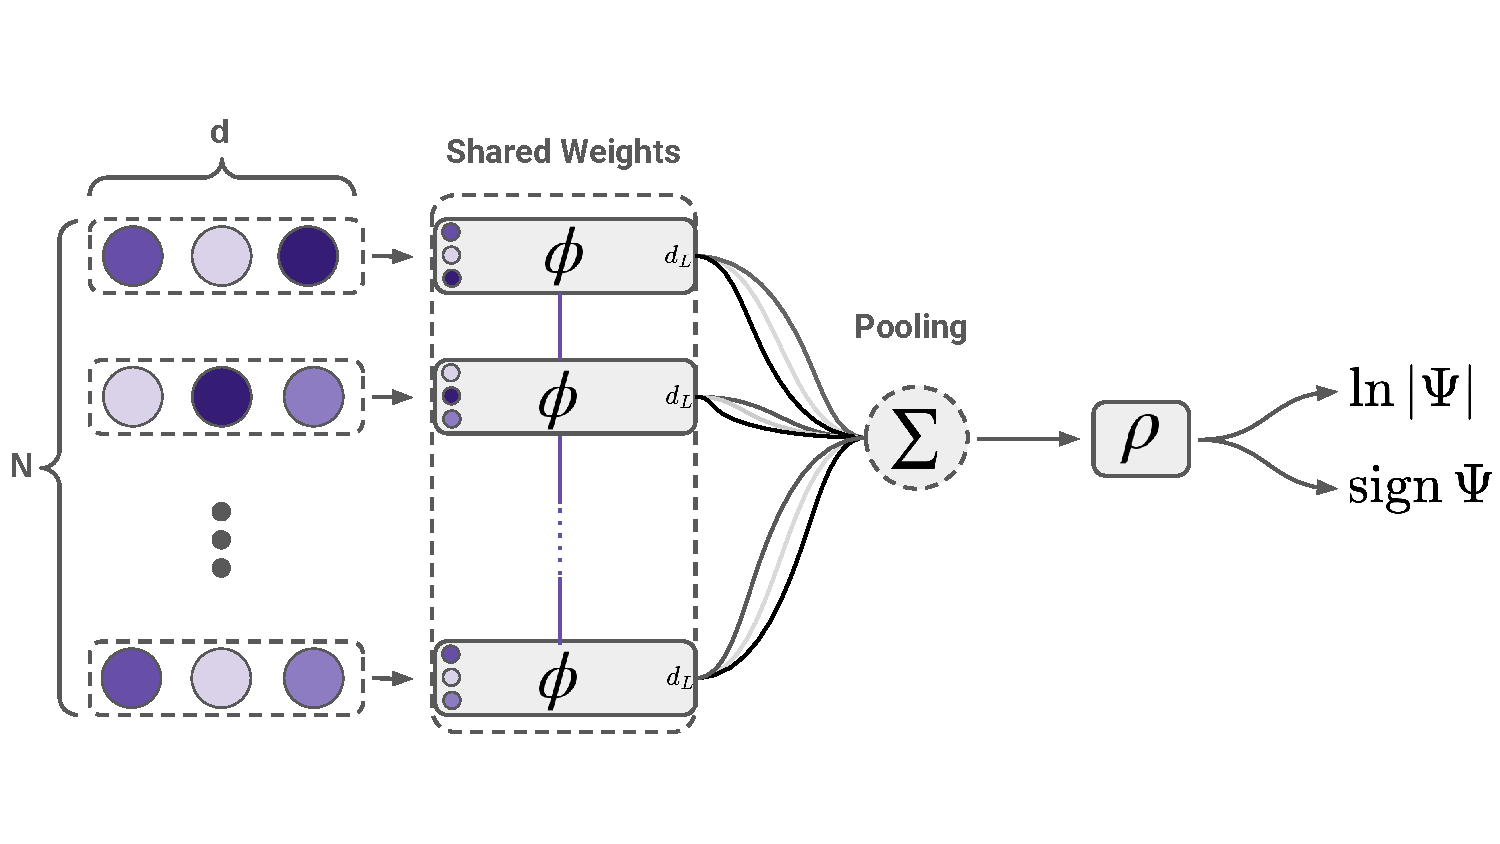
\includegraphics[width=0.9\linewidth]{Chapters/Methods/images/deepset_img.pdf}
    \caption{Representation of a permutational invariant Deep Set architecture. Figure inspired by \cite{jane}.}
    \label{fig:deepset}
\end{figure}

The core idea is that the pooling layer eliminates the specific particle-coordinate association, while the shared weights could theoretically learn inter-particle correlation and encode it to the latent space. This approach scales better than a brute-force symmetrisation in which one sums the outputs for all permuted configurations.

Then, in our code we proceed to use this architecture as the Gaussian envelope, exactly as in the aforementioned methods. Once again, $\psi_{\mtheta}^{(\text{ds})}(\mathbf{R})$ can be multiplied by a Slater-Jastrow or a Padé-Slater-Jastrow factor, yielding
\begin{align*}
    \ln \Psi^{(\text{ds})}_{S} &= \ln|\psi^{(\text{ds})}_{\mtheta}(\mathbf{R})| + \ln\left|\det\{H_{j}(\mvec{r}_i)\}\right|, \\ 
    \ln \Psi^{(\text{ds})}_{SJ} &= \ln \Psi^{(\text{ds})}_{S} + \mathcal{J}_{\mvec{\alpha}}(\mathbf{R}) ,\\ 
    \ln \Psi^{(\text{ds})}_{PSJ} &= \ln \Psi^{(\text{ds})}_{S} + \mathcal{P}_{\alpha}(\mathbf{R}). 
\end{align*}

\subsection{One and Two-Body Densities}

One typical way to analyse many-body correlations is via the one-body density matrix (OBDM),
\begin{align*}
    \rho(\mvec{r}'_1,\mvec{r}_1) = N \int d\mvec{r}_2 \ldots d\mvec{r}_A \Psi^*(\mvec{r}'_1, \mvec{r}_2, \ldots, \mvec{r}_N) \Psi(\mvec{r}_1, \mvec{r}_2, \ldots, \mvec{r}_N),
\end{align*}
which describes the probability amplitude of finding a particle at position $\mvec{r}_1$ while another one is at $\mvec{r}_1'$. For simplicity of visualisation, we have mainly been generating profiles of the diagonal of the OBDM, or the one-body density profile:
\begin{align*}
    n(\mvec{r}_1) = \rho(\mvec{r}_1, \mvec{r}_1) = N \int d\mvec{r}_2 \ldots d\mvec{r}_N \left|\Psi(\mvec{r}_1, \mvec{r}_2, \ldots, \mvec{r}_N)\right|^2 .
\end{align*}

These were obtained by keeping the post-training Monte Carlo sampled positions and displaying on an extra axis the count of how many instances fall under each bin after a discretisation of the space. This will yield a regular histogram for a one-dimensional system or a three-dimensional histogram for a two-dimensional system. The histogram can be normalised so that the density profile integrates to $N$. This is easily done with the NumPy \verb|histogram| function. For the three-dimensional histogram, we further smoothed the plot via a Gaussian filter.

Similarly, the two-body density matrix (TBDM), is a good way to identify higher-order correlation, and is given by
\begin{align*}
    \rho(\mvec{r}'_1,\mvec{r}'_2,\mvec{r}_1, \mvec{r}_2) = N(N-1) \int d\mvec{r}_3 \ldots d\mvec{r}_A \Psi^*(\mvec{r}'_1, \mvec{r}'_2, \ldots, \mvec{r}_N) \Psi(\mvec{r}_1, \mvec{r}_2, \ldots, \mvec{r}_N).
\end{align*}

Its diagonal gives the probability of simultaneously finding two particles at these designated positions $\mvec{r}_1,\mvec{r}_2$:
\begin{align*}
    n^{(2)}(\mvec{r}_1, \mvec{r}_2) = N(N-1) \int d\mvec{r}_3 \ldots d\mvec{r}_N \left|\Psi(\mvec{r}_1, \mvec{r}_2, \ldots, \mvec{r}_N)\right|^2.
\end{align*}

These quantities can be obtained similarly to the OBD profile, where we now bin unique pairs of particle positions. The caveat is that, if using Cartesian coordinates, we would gain a four-dimensional plot, impossible to visualise. However, we can proceed as \cite{Nordhagen2019} and use the radial symmetry of the harmonic trap, reduce the two spatial coordinates to a radial one and disregard the angle. For the sake of visualisation, we then replicate the profile obtained in the four quadrants.


\section{Computational Differentiation}\label{sec:cd}

The methods we employ throughout the thesis have a heavy dependence on the calculations of differentials.

When the derivative of a function is either unknown or we prefer not to calculate it analytically, there are various methods available through computational tools. We will consider computational differentiation to encompass finite difference (FD) methods, symbolic differentiation (SD), and automatic differentiation (AD). When analytical expressions are available, it is advisable to use them rather than rely on computational derivative calculations. This approach will not only be usually quicker but also mitigate the inherent loss of precision that comes with other computational methods.

Each of the above three methods has its advantages and drawbacks. The following is a brief generalisation of some of the important points. One can generally say that symbolic differentiation is inefficient but powerful in that it gives the form of the derivative function to the user. SD is also the best computational method when it comes to sparsity (for example, when a Jacobian matrix is sparse).

Numerical differentiation, together with the related finite difference methods, allows for some control over the precision versus performance trade-off. FD gives a quantification of the precision loss and good generalisability to higher-order differentiation, yet it is dependent on an appropriate and problem-specific choice of step size. The wrong choice leads to large round-off errors in what is called catastrophic cancellation.

For our calculations, except in cases where analytical expressions are used, the method of choice will be AD. AD is very fast and precise and is especially suited to gradient-based optimisations. This is because AD is fast when dealing with partial derivatives with respect to multiple inputs. AD operates by taking advantage of the computational graph that is created when a computer composes simpler arithmetic operations to compute any function. The presence of this composition-like structure in a computer programme enables a straightforward application of the chain rule of partial derivatives to arrive at the final solution. To do that, of course, the programme needs to have access to the function itself, so this method is not applicable in situations where the function is a black box\footnote{Not in the same sense as machine learning black-box but in the sense that the computer has no access to the instructions to be performed for the function output calculation.}.

\subsection{Automatic Differentiation}\label{sec:ad}
Automatic differentiation exists in two variations: forward mode and reverse mode. Understanding this is relevant, especially to explain why our Hessian implementation is actually very efficient. Consider a function $\mathcal{L} : \mathbb{R}^n \to \mathbb{R}^m$, where we write $\mathcal{L}(\mvec{x_0}) = \mvec{y}$. We will denote its Jacobian evaluated at a point $\mvec{x_0}$ in the domain as $\partial_{\mvec{x}} \mathcal{L}(\mvec{x_0}) \in \mathbb{R}^{m \times n}$, or in matrix form:
\begin{align*}
    \partial_{\mvec{x}} \mathcal{L}(\mvec{x}_0) = \begin{pmatrix} \partial_{x_1} y_1 & \partial_{x_2} y_1 & \cdots & \partial_{x_n} y_1 \\ \partial_{x_1} y_2 & \partial_{x_2} y_2 & \cdots & \partial_{x_n} y_2 \\ \vdots & \vdots & \ddots & \vdots \\ \partial_{x_1} y_m & \partial_{x_2} y_m, & \cdots & \partial_{x_n} y_m \end{pmatrix}.
\end{align*}

That function, when calculated in a machine, will be a result of the composition of, for example, $k$ simpler functions $\mathcal{L} = f_k(\cdots f_3(f_2(f_1(\cdot))))$. When applying the chain rule to evaluate the total derivative of $\mathcal{L}$, it is then
\begin{align}
    \partial_{\mvec{x}} \mathcal{L} (\mvec{x}_0) &= \left(\left(\left(\left(\partial_{f_{k-1}} f_k  \partial_{f_{k-2}} f_{k-1} \right)\cdots \partial_{f_{2}} f_{3}\right) \partial_{f_{1}} f_{2}\partial_{\mvec{x}}\right) f_{1}(\mvec{x_0})\right) \label{eq:ad_backward}\\
    &=\left(\partial_{f_{k-1}} f_k \left( \partial_{f_{k-2}} f_{k-1} \cdots \left(\partial_{f_{2}} f_{3} \left(\partial_{f_{1}} f_{2}\partial_{\mvec{x}} f_{1}(\mvec{x_0})\right)\right)\right)\right)\label{eq:ad_forward}
\end{align}

The distinction in computational order between \eqref{eq:ad_backward} and \eqref{eq:ad_forward} is exactly what differentiates forward mode AD from backward mode AD.
When one evaluates the computations from inside-out in terms of the order of the compositions, this is called forward mode. 

The Jacobian itself is a linear transformation and can be seen as a function $\partial f :\mathbb{R}^n \to \mathbb{R}^m$. Furthermore, the chain rule of the Jacobians is, in fact, a set of matrix multiplications. Therefore, while being mathematically equivalent, forward and backward modes do not have the same computational complexity in terms of floating-point operations. Which one is more efficient depends on the problem at hand. For example, if $x\in \mathbb R^{N_0}, f_1\in\mathbb R^{N_1}, \dots, f_k\in\mathbb R^{N_k}$
, backward AD is typically faster if $N_k >N_0$. If $N_k < N_0$, forward AD is favoured \cite{bradbury2018jax}.

From \secref{sec:VMC} we see that VMC will rely on several Laplacian computations, which can be obtained via traces of Hessian matrices. When calculating elements of a Hessian, performing a forward mode over a reverse mode AD or the other way around would both be possible paths. In machine learning applications, however, the function we differentiate often has a wide Jacobian, since a loss function commonly maps to a real number, $\mathcal{L}: \mathbb{R}^n \to \mathbb{R}$. That is why several AD functions are built in reverse mode. Despite that, a Hessian calculation involves the Jacobian of a Jacobian. Since the inner Jacobian will commonly be wide, differentiating it will be better suit for forward mode. Then, forward-over-reverse tends to be more efficient, and this is how we proceed. 

There is of course a case to be made about memory cost. Generally speaking, forward AD is favoured when a neural network is very deep because backward AD requires the storage of more Jacobian matrices.

\section{Just in Time Compilation}\label{sec:jit}
Our current work is done in the Python programming language. This choice is motivated by numerous advantages that Python offers for scientific programming and machine learning, one of which is flexibility, but to the detriment of speed. Although it has had significant improvements in performance in the last years, it still falls short in comparison to purely compiled languages like C++ and Fortran. 

Python has elements of compiled and interpreted languages, and the process of running a Python script can be broadly divided into two parts. First, the source code is compiled by CPython into a lower-level language, bytecode. Bytecode is simply a platform-independent representation of the code but is not yet machine code, and therefore Python is not compiled in the traditional sense. Subsequently, there is an interpretation stage, where the bytecode is fed to a virtual machine. This final stage includes processes such as dynamic type checking and memory management components, along with certain features that offer flexibility but can compromise performance.

Fortunately, with specific tools and some change in code structure, it is possible to compile bytecode to machine code of some functions at runtime - a process called just-in-time (JIT) compilation. JIT compiled functions can be run directly by hardware, helping with interpretation overhead and allowing compiler optimisation and accelerated linear algebra (XLA) techniques to take place. This is particularly valuable in scientific programming, where functions are essentially static, often computationally costly, and must be executed countless times in a simulation.

The design choices that allow for the JIT compilation depend on the framework we use to do so, and there are several Python options. We better explain our JAX \cite{bradbury2018jax} implementation in \secref{sec:jax}, together with several points that require extra care when implementing JIT compilation.


\section{Codebase Overview}

All the code work for this thesis can be found in the Github repository \cite{NQSrepo} and, as it can be used as a Python package, a documentation page is available at \cite{NQSdoc}. The aforementioned pages also contain instructions on how to install the package and run the code. A conceptual representation of the codebase is illustrated in \figref{fig:nqs_overview}. Please note that this diagram does not perfectly map to the repository's modules and is intended to facilitate conceptual understanding. For a detailed view, we refer to the documentation page. We further disclaim that all results were generated on a Mac equipped with an M2 Pro chip and 16 GB of RAM. This machine displayed faster running times than any of the three clusters tested.


\begin{figure}[H]
    \centering
    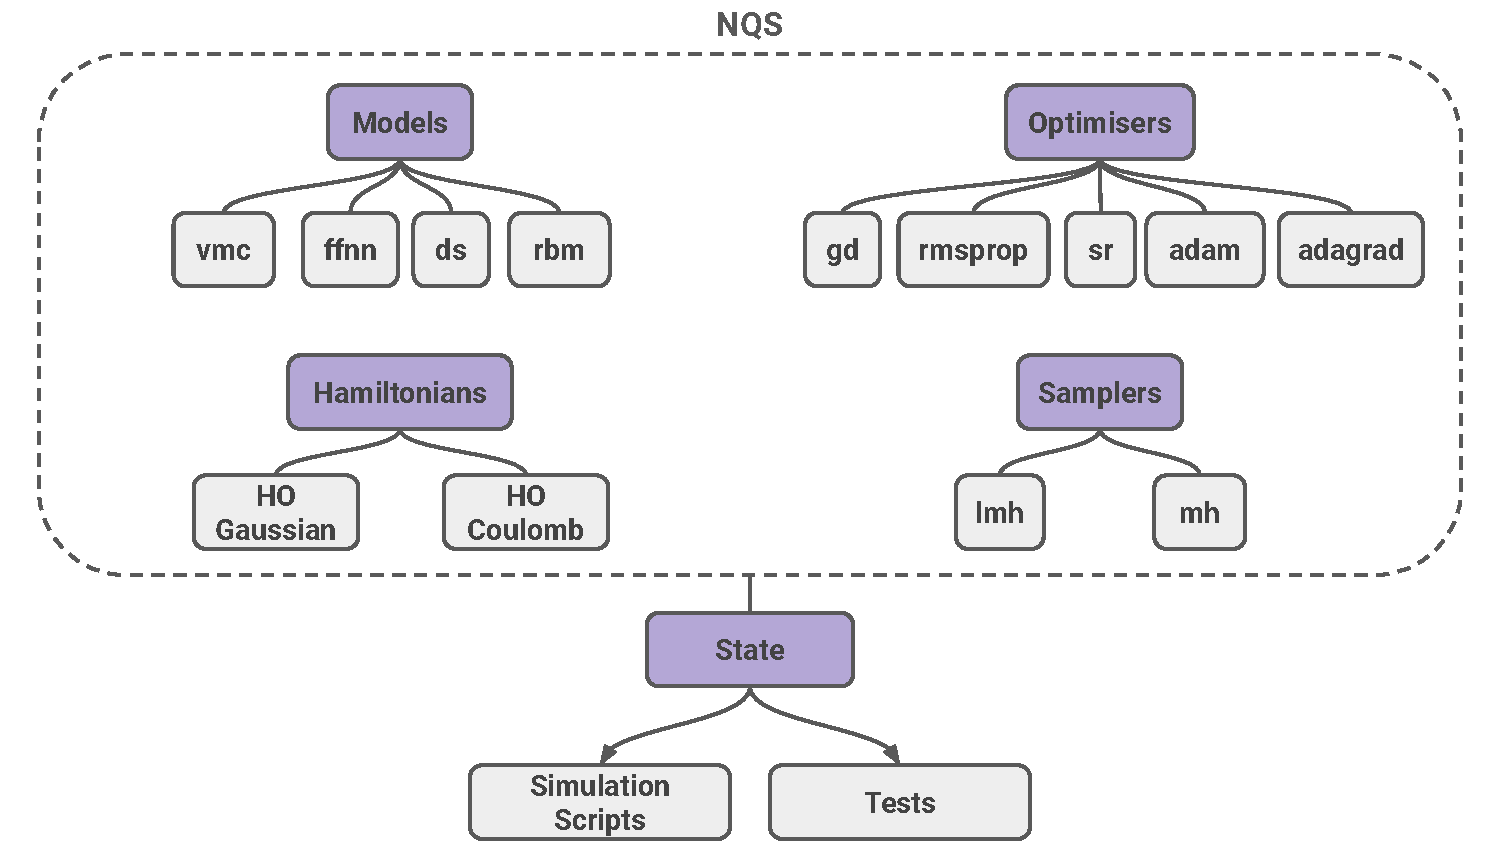
\includegraphics[width=\linewidth]{Chapters/Methods/images/codebase_overview.pdf}
    \caption{Conceptual overview of the NQS codebase, which can be found at \cite{NQSrepo}. See text for explanations.}
    \label{fig:nqs_overview}
\end{figure}

\subsection{Models}

In the project, the term 'models' refers to various choices of ansätze. We have implemented essentially four variants, but only show results for 3 of them. The options are a standard parametrised variational Monte Carlo (VMC), a restricted Boltzmann machine (RBM), a deep-set variant of a feed-forward neural network, and a standard feed-forward neural network for which we do not show results. All of these are implemented to represent the natural logarithm of the absolute value of the wavefunction, for which the sign can always be retrieved with NumPy's function \verb|slogdet|. All models can also be accompanied by a Jastrow factor or a Padé-Jastrow factor.

\subsection{Optimisers}
Following the idea of a modular project, all opitimisers can be used with every model or system, and five options are included: gradient descent (\verb|gd|), adaptative moment estimation (\verb|adam|), root mean square propagation (\verb|rmsprop|), adaptative gradient estimation (\verb|adagrad|) and stochastic reconfiguration (\verb|sr|). Their individual hyperparameters can also be freely modified via the same \verb|set_optimzier| method. 

It should be mentioned that the implementation of stochastic reconfiguration, when used for multilayer networks such as \verb|dsffn| and \verb|ffnn|, approximates the fisher information metric by a block diagonal matrix, as
per \cite{martens2015optimizing}, which we better explain in \secref{sec:kfac}. We chose to continue calling it \verb|sr| to keep consistency, since the VMC and RBM models technically do not use this approximation.

We here display the \verb|set_optimzier| method, and the associated \verb|optimizer_factory|.
\begin{lstlisting}
def set_optimizer(self, optimizer, eta, **kwargs):
    """
    Set the optimization algorithm for parameter updates in the NQS simulation.

    Parameters:
        optimizer (str): The optimizer to use (e.g., 'adam').
        eta (float): The learning rate.
        **kwargs: Additional keyword arguments for the optimizer.

    Raises:
        ValueError: If an unsupported optimizer is specified."""
    self._eta = eta
    common_args = {
        "params": self.wf.params,
        "eta": eta,
    }
    self._optimizer = optimizer_factory(optimizer, **common_args, **kwargs)
\end{lstlisting}

The \verb|optimiser_factory| is responsible for returning the correct class without polluting the main \verb|NQS| class.

\begin{lstlisting}
from nqs.optimizers import Adagrad, Adam, Gd, RmsProp, Sr


def optimizer_factory(opti_type, **kwargs):
    opti_type = opti_type.lower() if isinstance(opti_type, str) else opti_type

    match opti_type:
        case "gd":
            return Gd(**kwargs)
        case "adam":
            return Adam(**kwargs)
        case "rmsprop":
            return RmsProp(**kwargs)
        case "adagrad":
            return Adagrad(**kwargs)
        case "sr":
            return Sr(**kwargs)
        case _:  # noqa
            raise NotImplementedError(
                f"No options for {opti_type}, Only the gd, adam, rmsprop, adagrad and sr supported for now."
            )
\end{lstlisting}


\subsection{Hamiltonians}
The \verb|Hamiltonian| class allows for flexibility in the setup of the physical problem. Any type of particle interaction or external potential can be easily set up. Although it only contains one child class, \verb|HarmonicOscillator|, the type of interaction can be controlled and passed via the \verb|set_hamiltonian| method from the \verb|NQS| class. 

The class is accessed when the method \verb|local_energy| is invoked by the selected sampler, and the measurement is conducted on the wavefunction model object, which is our ansatz.

\subsection{Samplers}

The \verb|Sampler| base class has as child classes \verb|Metropolis| and \verb|MetropolisHastings|, where the latter implements the Langevin Metropolis-Hastings importance sampling described in \secref{sec:langevin_imporance}. 

The base class manages common functionalities, such as setting up the random number generator, logging, and handling the scale parameter for sampling resolution, while the child classes perform the method-specific sampling step. The base class also commands the spawning of parallel but individual Markov chain walkers together with the subsequent collection of statistics from the sampling.

It must be mentioned that our Monte Carlo samplings move all particles at the same time instead of one at a time. Although this is more efficient in terms of random number generation (a large bottleneck in any Monte Carlo calculation), it impedes us from using common tricks to speed up the determinant calculation, such as calculating the determinants via cofactors and updating individual determinant matrix columns. 


\subsection{State}
The State module combines all the pieces of the project in a large class, \verb|NQS|. There, some things can be chosen via their appropriate set methods, such as samplers, models, and optimisers. Although de do not want to include all these methods extensively here, their idea can be illustrated via the set optimser and \verb|set_wf|, the latter being responsible for choosing the ansatz.

\begin{lstlisting}
def set_wf(self, wf_type, nparticles, dim, **kwargs):
    """
    Set and initialize the wave function for the NQS simulation.

    Parameters:
        wf_type (str): The type of wave function to use.
        nparticles (int): The number of particles in the system.
        dim (int): The dimensionality of the system.
        **kwargs: Additional keyword arguments for the wave function initialization.

    Raises:
        ValueError: If an invalid wave function type is provided.
    """
    self.N = nparticles
    self.dim = dim
    self._particle = kwargs.get("particle", "none")
    common_args = {
        "nparticles": self.N,
        "dim": self.dim,
        "rng": self.rng(self._seed) if self.rng else np.random.default_rng(),
        "logger": self.logger,
        "logger_level": "INFO",
        "backend": self._backend,
    }
    specific_args = kwargs
    self.wf = wf_factory(wf_type, **common_args, **specific_args)
    self.nqs_type = wf_type
    self._is_initialized_ = True
\end{lstlisting}

\subsection{Backend}\label{sec:jax}
One of the first things to choose in the NQS class is the back-end, for which the two available options are NumPy \cite{harris2020array} and JAX. In the former, the analytical expressions for the gradients and Laplacians of the ansatz are used, which enables a significant speedup in comparison to JAX automatic differentiation (AD).  However, having the analytical expressions for the gradients is not always straightforward and can limit the great flexibility of deep networks. In our code, using JAX as a back-end is always possible, while NumPy is only allowed for the standard VMC and RBM ansätze, as their analytical expressions can be easily obtained beforehand.

Fortunately, JAX's just-in-time (JIT) compilation speeds up the code considerably, especially when implemented correctly with vectorised maps (vmaps). While we explain AD and JIT in \secref{sec:cd} and \secref{sec:jit}, vmaps are essentially JAX's way of using vectorisation to gain efficiency and readability. 

Unfortunately, extracting JAX's full power requires dealing with some ``sharp bits", in the own words of the project developers. Although we acknowledge that our code may not follow the absolute best practices, it is still relevant to address some of these challenging aspects. For a deeper explanation, we highly recommend the source code and documentation of the framework \cite{bradbury2018jax}.

First, JAX transformations and compilations only work with functions without side effects. This means that ``jitted'' functions, for example, should not modify class attributes or methods if those are not passed as input parameters. This can seem straightforward, but is sometimes difficult to implement when the code design is around object orientation. This requirement of functionally pure code is the reason behind some of the unusual choices in our code, and can be difficult to debug.

Moreover, JAX arrays are immutable and inplace updates need to be substituted from \verb|x[idx] = y| to \verb|x.at[idx].set(y)|. In fact, JAX functions do not deal with NumPy arrays. Fortunately, they are automatically converted to JAX arrays with little to no overhead. 

The minor overhead is the reason we were lax with our array initialisation. For best practices, it would have been preferable to specify the type of array the code is handling from the start, but more often than not, we opted to start with NumPy arrays and let JAX handle the rest. This point is also relevant because we decided not to use JAX's PRNG even when using it as a back-end. 

JAX's RNG is significantly slower than Numpy's defaults, and while there are very good reasons for it, that was not relevant for how we developed our code. We instead leave PRNGs with NumPy, use JAX only for JIT, vmaps and AD, and suffer the overhead from multiple NumPy-to-JAX conversions. In our experience, this was still preferable to using JAX's PRNG.


\subsection{Parameter Class}

We implement the neural nets from scratch, and without pre-built neural network modules. Then, since we want to have a consistent structure for all the possible variational ansatz, we decided to have a specific parameter class.

The \verb|Parameter| class is initialised with a dictionary where the keys are strings representing parameter names, and the values are the parameter data, which can be either NumPy arrays or JAX arrays. This allows for a flexible and extensible structure to hold various types of parameter data.

\begin{lstlisting}
ParameterDataType = Union[np.ndarray, jnp.ndarray]

class Parameter:
    def __init__(self, data: Dict[str, ParameterDataType] = None) -> None:
        self.data = data if data is not None else {}

\end{lstlisting}

The class provides several methods for setting, getting, and manipulating parameter data. The set method is particularly versatile, allowing for setting parameters using different types of input: Replacing the entire parameter data with another Parameter instance, setting multiple parameters using lists of names and values, updating or adding parameters using a dictionary or setting a single parameter using a name and value pair.
\begin{lstlisting}
def set(
    self,
    names_or_parameter: Union[
        str, List[str], "Parameter", Dict[str, ParameterDataType]
    ],
    values: Union[ParameterDataType, List[ParameterDataType]] = None,
) -> None:
    # Method implementation...
\end{lstlisting}

Then, the get method retrieves the value of a parameter specified by name, in the optimisation step. To exemplify, a step of a gradient descent with momentum follows:
\begin{lstlisting}
def step(self, params, grad_params_E):
    for key, grad in grad_params_E.items():
        self.v[key] = self.gamma * self.v[key] + grad
        params.set([key], [params.get(key) - self.eta * self.v[key]])
\end{lstlisting}

One of the key aspects of this class is its integration with JAX's tree utilities, which is essential for enabling JAX's automatic differentiation and other optimisations. The \verb|tree_flatten| and \verb|tree_unflatten| methods are implemented to allow the Parameter class to be used with JAX's \verb|jit|, \verb|grad|, and other transformations. The \verb|tree_flatten| method breaks down the Parameter object into a list of its values (leaves) and a list of keys (auxiliary data). This decomposition is necessary for JAX to understand and manipulate the data structure during computation.

Finally, the \verb|Parameter| class is registered with JAX using the \verb|register_pytree_node| function. This registration tells JAX how to handle instances of the \verb|Parameter| class during its computations.

\subsection{The Wavefunction Base Class}

The \verb|Wavefunction| base class is inherited by any choice of ansatz or model, allowing for modularity. Its design ensures that common functionalities are handled in one place while allowing specific behaviours to be defined in child classes. It, for example, controls, via abstract class methods, the setput of the Slater determinants and the Jastrow factors regardless of the trial function. This is because specific methods are called in the constructor of its child classes.

Very importantly, too, this class enables the setup of the appropriate backend (NumPy or JAX), and the just-in-time compilation for the appropriate functions. 

\subsection{Simulation Scripts}

The simulation scripts in this repository manage the entire simulation process. They outline the steps for initialising models, configuring Hamiltonians, choosing and executing samplers, carrying out optimisation, and also gathering the results. These scripts are created to be modular and flexible, enabling easy modification of parameters and settings. This means that almost all options can be arbitrarily combined. For example: any model can take any particle type and use any optimiser, any sampler, and any Hamiltonian. We refer to Appendix \ref{sec:minimal_nqs} for a minimal display of one of these simulation scripts.




\section{General Training Strategies}

In this section, we present a variety of implementation techniques that were crucial to achieving satisfactory results.

\subsection{Pretraining and regularised potential}\label{sec:pretrain}

Throughout our implementations, we make use of the method of transfer learning. Transfer learning consists in loading the weights of a model trained in a similar problem to accelerate the convergence when using the network in other scenarios. More specifically, this was a crucial step in obtaining reasonable convergence when minimising the energy of interactive systems with multilayer network ansatz. In dimensions larger than 1, we did not manage to get stable sampling without it, giving positions in a clearly unbounded way.

First, we pretrain the network to a supervised regression task, in which we regress the log-probability $\ln(|\psi|^2)$ of the ansatz to the log of a multivariate Gaussian with identity covariance matrix of dimension $(N\times d) \times (N\times d)$, where $N$ is the number of particles, and $d$ the number of dimensions. This is to ensure that the network at least starts with a function with a vanishing profile for large coordinate values.

The second stage involves either pretraining the network to the non-interactive related system, or training in a regularised potential that converges to the true interaction potential towards the end of the training process.

Both these second-stages consist in training the model within the standard VMC - reinforcement learning framework, but the details vary based on the system. If the particle interaction does not exhibit singularities, we pretrain the ansatz to converge to the non-interacting system. Else, we regularise the potential, adopting a method inspired by \cite{jane}.
While this regularisation and pretraining are different techniques, the regularisation process essentially introduces the interaction slowly and in a specific way that hopefully helps the network learn Kato's cusp condition without the need to impose a fixed Jastrow factor. This regularisation consists of using a potential
\begin{align*}
    \frac{1}{r_{ij}} \to \frac{\tanh(r_{ij}/r_0)}{r_{ij}}
\end{align*}
where $r_0$ is a hyperparameter. The numerator in this regularisation can be any function of $r_{ij}$ such that $f(r_{ij})$ approaches 1 as $r_{ij}$ approaches 0. 
More specifically, in our implementations we add a decay rate $\tau$ to $r_0$,
\begin{equation}
    \tau = \left(\frac{1}{3 r_0}\right)^{2/T},
\end{equation}
such that, at half of the training process, $\tanh(r_{ij}/r_0) \approx 0.97$. Here, $T$ is the total number of training epochs, and at each iteration, we change $r_0(t) = r_0(0)\cdot\tau^t$, where $t$ is the current epoch. When sampling the observables from the final ansatz after training is done, we simply turn off this regularisation so that the ansatz is kept fixed.

\subsection{Sampler Tuning}

The quality of a Monte Carlo sampling is heavily influenced by the width of the distribution that is sampled from. In our implementations, this width is simply called the scale of the Monte Carlo method. In order to obtain an efficient sampling process, one usually aims at finding a sample width that yields approximately 50\% of accepted moves. To achieve that, we created a \verb|tune_scale| method based on the PyMC library \cite{pymc2023}, but with some minor modifications.

In the PyMC implementation, the method adjusts the proposal scale for a sampler based on the acceptance rate, aiming for an optimal range between 20-50\%. Our approach differs by targeting an acceptance rate of 50-70\%. Furthermore, our method activates only when the acceptance rate falls outside the 30-70\% range, to avoid unnecessary tuning. These target values were determined experimentally, without a rigorous experimentation process.

The tuning process operates via a lookup table that adjusts the proposal scale according to predefined acceptance rate thresholds. If the acceptance rate is extremely low (<0.001) or extremely high (>0.99), we reinitialize the sampling positions and the weights of the ansatz without stopping the training process. This decision comes from observing that such acceptance rates indicate that the walkers have wondered into regions of impossible convergence, often due to an ill-defined ansatz.

When tuning the sampler, some considerations must be made. One of these is the batch size used to evaluate the acceptance rate. This batch size can be larger than the training batch size for higher precision in the tuning phase or smaller for faster execution. Another key consideration is whether to exit the tuning process if the optimal acceptance rate range is not met.

To address this last point, we devised two methods for the tuning process. The standard method allows setting a maximum number of iterations for the tuning process. If the acceptance rate does not fall within the optimal range within these iterations, the process stops. In contrast, the infinite method continues the tuning indefinitely until the acceptance rate falls within the desired range.

\subsection{Clipping gradients and energy values}
Lastly if should be mentioned that we implemented clipping strategies in two instances to obtain numerical stability. First, following an approach similar to \cite{ferminet}, the local energy values during network training are clipped according to the $\ell_1$ norm. Specifically, the average local energy $\langle E_L\rangle $ is kept only if it falls within the range $\langle E_L\rangle \pm 5 \times \langle | E_i - \langle E_L\rangle |\rangle$.

Another strategy that was implemented by us but not thoroughly examined was gradient clipping. Gradient clipping consits in rescalling the gradient vectors to have a smaller norm, while still pointing to the same direction in space. This has been shown to help with training convergence in regions where the loss landscape has abrupt changes. Essentlially it consits in defining a threshold $\rho$ and redefining $ \nabla \mathcal{L}$ if $\norm{\nabla \mathcal{L}} > \rho $ to 
\begin{equation}
    \nabla \mathcal{L} \leftarrow \frac{\rho \nabla \mathcal{L} }{\norm{\nabla \mathcal{L}}}.
\end{equation}


\subsection{Parallelisation}\label{sec:parallel}

Good statistics of the quantities obtained via Monte Carlo simulations are heavily dependent on how much data we are able to generate. Assuming that the simulated data represent independent and identically distributed sub-samples of the quantity we are trying to infer, the law of large numbers ensures that having a larger number of points will result in a better reconstruction of the true probability distribution.

One reliable way to obtain more data for Monte Carlo simulations in a similar amount of time is to collect samples from parallel random walkers. This means that simulations are run in parallel and that their individual sampled values can be combined to compose a larger collection of the final data. One important assumption for this parallelisation process is that random walkers are unaware of each other, so the samples do not exhibit undesired correlations, compromising the statistical significance of the computations. This requirement can be satisfied by passing unique random seeds for the different threads of the parallel programme. 

In particular, for our Python parallel sampler implementation, we used the Joblib \cite{joblib} library. The motivation for using Joblib instead of Python's native multiprocessing module is that the latter displayed problematic behaviour when sharing JAX objects among processes. Joblib's \verb|parallel| function achieves embarrassingly simple parallelisation by starting separate Python workers that execute tasks on different CPUs.


\section{Quantifying uncertainties}\label{sec:blocking}
There are multiple ways to analyse the statistical uncertainty of the collected data. Most standard methods rely on resampling techniques, which artificially generate more data by creating varied samples from the limited data set. For example, by shuffling data and resampling it, one can achieve a finer statistical estimation of the measured quantities due to the larger amount of data, hopefully without biasing it too much.

Conventional implementations include bootstrapping and cross-validation, better explained in \cite{hastie2009elements}. VMC calculations deal with a very large amount of data, making these approaches computationally costly. More importantly, perhaps, these methods also do not explicitly take into account the correlation between data points, an important feature when analysing how the random walks evolve in configuration space. Of course, at a stationary limit, sample averages should be time independent, but in practice we do not have this guarantee. Therefore, specifically for VMC calculations, the blocking method is often used. 
 
Quantities measured in a Monte Carlo sampling are the results of a set of sequential experiments, $\{\alpha\}$. The sampled values, such as the mean ($\mu_\alpha$) and variance ($\sigma_\alpha^2$) of these experiments, can therefore be studied as a time series. Here, these quantities are given by
\begin{equation}
    \mu_{\alpha}=\frac{1}{N}\sum_{k=i}^N x_{\alpha, k}, \qquad \sigma^2_\alpha=\frac{1}{N}\sum_{k=1}^N(x_{\alpha, k} -\mu_\alpha)^2.
\end{equation}

The entire data set can be partitioned into $m$ experiments blocks, with its $m$-th block having an average $\mu_{m}$ with a sample mean variance $\sigma^2_m$; both can be written as
\begin{align}
    \mu_{m}=\frac{1}{mN}\sum_{\alpha, k} x_{\alpha, k}, \qquad  
    \sigma^2_m= \frac{\sigma^2}{N}[1 + 2\sum_{d=1}^{N-1}k_d],
    \label{eq:blocking_std}
\end{align}
where $\sigma^2$ is the variance of all the data points,
\begin{equation*}
    \sigma^2 =\frac{1}{mN}\sum_{\alpha k}(x_{\alpha, k} -\mu_m)^2,
\end{equation*}
and $k_d$ is the autocorrelation function \cite{park2018fundamentals} between experiments separated by a distance of $d$ in the time series. The blocking algorithm consists of rearranging the total data set into blocks and analysing how $\sigma_m^2$ changes with different block sizes. When the number of blocks increases, this variance of the average of the blocks reaches a plateau that gives information about the correlation of the experiments. The aim is to find a distance $d = |k-l|$ between sequential experiments $x_{\alpha, k}$ and $x_{\alpha, l}$ such that experiments in the time series separated by a distance $d' > d$ can be considered uncorrelated. The standard deviation provided by the blocking algorithm will then be the asymptotic value that stabilises for this distance $d$. This is clear from \eqref{eq:blocking_std}, as $\sigma^2_m \to \sigma^2/N$ if $k_d$ tends to 0.

In our implementation of the blocking algorithm for the estimation of the standard deviation of the energy, we used the systematised scheme of \cite{jonssonStandardErrorEstimation2018}. This method automates the ordinary visual analysis of the time auto-correlation function devised by \cite{flyvbjergErrorEstimatesAverages1989}. 

\subsection{Combining errors}
We have discussed the use of parallelisation techniques in Python to produce more samples in roughly the same time frame via parallel computing and multiple CPUs. Here, we give a more detailed explanation of how we aggregated the errors from each independent experiment.

The empirical expected values and their variances are also random variables, and to appropriately combine mean values and standard errors, we used a meta-analysis study. More specifically, we use inverse variance weighting (IVW) \cite{borenstein2021introduction} to aggregate the values of random variables so that their average is weighted by the inverse of their variance.

After running $n$ independent walkers, each will give us an empirical expectation value of the energy $E_n$, with its associated blocking error $\text{SE}(E_n)$. Then, we use IVW to combine these values into a single overall estimate of energy $\bar{E}$ and its associated error $\text{SE}(\bar{E})$ as follows:
\begin{equation*}
\bar{E} = \frac{\sum_{i=1}^n w_i E_i}{\sum_{i=1}^n w_i},
\end{equation*}
with the weights determined by the inverse variance of each estimate $w_i = \text{SE}(E_i)^{-2}$. Then, the standard error of the mean estimate is given by
\begin{equation*}
\text{SE}(\bar{E}) = \sqrt{\frac{1}{\sum_{i=1}^n w_i}}.
\end{equation*}

\section{Kronecker-factored Approximate Curvature}\label{sec:kfac}

In practical applications, particularly with the emergence of deeper and broader networks in deep learning, calculating the complete Fisher information matrix or its quantum counterpart, the Fubini study metric, becomes impractical. Not only is it computationally demanding to invert the matrix $F_{ij}$ as required by the update rule, but storing the matrix elements also becomes memory intensive. Indeed, in a naive approach, one must recompute and store its values for each training iteration. 

If we consider a rectangular neural network structure, in which all $L$ layers have the same height $H$, and further assuming that there are no bias vectors, the FIM should be a matrix of size $(L \times H^2) \times (L \times H^2)$. Kronecker-factored approximate curvature (KFAC), devised by Martens and Grosse in 2015 \cite{martens2015optimizing} is a technique that aims to simplify this structure in two ways. In this brief explanation, we do not provide a derivation of the expressions, and for a detailed proof, we refer to the original publication.

Using the notation of \cite{drissi2024second}, we start by approximating the FIM by a block-diagonal $\breve{F}$,
\begin{align}
    \breve{F}(\mvec{\theta})_{W_{ij}^{(l)}{W^{(l')}_{i'j'}}} \equiv \delta_{ll'}\, F(\mvec{\theta})_{W_{ij}^{(l)}{W^{(l')}_{i'j'}}},
\end{align}
where $W_{ij}^{(l)}$ represents a weight matrix of given layer $l$, and $\delta_{ll'}$ a Kronecker delta. This means that we assume parameters from different layers of the network to be independent in terms of the curvature of the parameter space. This turns the $(L \times H^2) \times (L \times H^2)$ matrix into $L^2  H^2$ blocks of $(H\times H)$ matrices that can be inverted independently.

The second simplification of the KFAC method consists of writing the blocks of the approximated $\breve{F}$ as Kroneker products of statistical averages of the forward activations $\Vec{a}^{(i)}$ and backward sensitivities $\delta^{(i)}$ of the FFN, discussed in \secref{sec:training a FFN}. Then, it can be shown that 
\begin{align}
    \breve{F}(\mvec{\theta})^{(l)} \approx \mathbb{E}_{p_\theta}\left[\Vec{a}^{(l)}\Vec{a}^{(l-1)^\top}\right]\otimes\mathbb{E}_{p_\theta}\left[\delta^{(l)}\delta^{(l-1)^\top}\right].
\end{align}
However, throughout this work, we do not implement this last simplification.

\subsection{Trust regions and Tikhonov regularisation}

When solving second-order optimisation problems practically, the constrained minimisation problems of \eqref{eq:steepst_argmin} and \eqref{eq:newtons_minimisation}, discussed in \secref{subsec:Learning as opt} are often treated as analogous unconstrained problems with associated trust regions and damping parameters, in what is called the Tikhonov regularisation method. More specifically, consider the second-order approximation model
\begin{equation*}
M(\delta) = E(\boldsymbol{\theta}_0) + \nabla E(\boldsymbol{\theta}_0)^\top \delta + \frac{1}{2} \delta^\top G \delta,
\end{equation*}
where 
$\delta = \mvec{\theta} - \mvec{\theta}_0$ , and 
$G$ is a matrix describing the geometry of the trust region. For example, in Newton's method, it is the Hessian of the objective function, and in the natural gradient method, it is the Fisher information matrix. Following Tikhonov regularisation, the correct update rule is given by the unconstrained minimisation,
\begin{align*}
    \mvec{\theta}_{t+1}- \mvec{\theta}_t = \arg \min_{\delta\in R_t} \left(M_t + \frac{\lambda_t}{2} \delta^\top G(\theta_t)\delta\right),
\end{align*}
where, $\lambda$ is the damping term and $R_t = \{\delta : \norm{\delta} \le r_t\}$, for some radius $r_t$, is a trust region for which the second-order approximation is valid. Adding this damping term has the effect of using a regularised version of the FIM, equivalent to $F - \lambda I$. This is important to stabilise the pseudo-inverse calculation of $F$ via singular value decomposition. In our work, we have used a diagonal shift of around $\lambda = 10^{-4}$.

In reality, choosing the correct radius of the trust region at every step is impractical, and learning rate decay schedules have been suggested to ameliorate this difficulty \cite{glasser2018neural}. For our implementations, we proceeded by choosing the learning rate
\begin{equation*}
     \alpha_t = \min\left(\alpha_0, \sqrt{\frac{\alpha_1}{\delta_\theta^\top G \delta_\theta}} \right)= \min\left(\alpha_0, \sqrt{\frac{\alpha_1}{(F^{-1} \nabla E(\theta))^\top \nabla E(\theta)}} \right),
\end{equation*}
with $\alpha_0$ and $\alpha_1$ hyperparameters that require tuning. This is an idea suggested in \cite{sheng}, which requires that the scheduler choice could depend on the curvature of the trust region. This choice ensures that the learning rate is smaller when the curvature of the parameters under the metric defined by $G$ is large. In addition to that, we also added a momentum term of $\gamma = 0.9$ in our implementations. Then, the update rule when implementing specifically our version of SR can be written 
\begin{align*}
    \mvec{v}_t &= \gamma \mvec{v}_{t-1}  + \breve{F}^{-1}\nabla E(\theta), \\
    \mvec{\theta}_{t+1} &= \mvec{\theta}_{t} - \alpha_t\mvec{v}_t,
\end{align*}
where we denote $\breve{F}$ as the block-diagonal approximation of the FIM.

\section{Hyperparameter Search}\label{met:param_search}

Optimising hyperparameters is a crucial part of training machine learning models, as it can greatly influence the quality of the model. Performing extensive brute-force searches over the hyperparameter space is a task that is intractable on its own, as the number of possible configurations scales exponentially. To find the best configuration for a certain model, several techniques can be employed, the simplest being random selection over the parameter space. 

Several of our initial investigations to find a good choice of model and parameters begin with a trial-and-error process, as this carries a lower overhead in initial iterative phases of a project. However, for more detailed and subsequent investigations, when the aim is to find the best model, we utilised the Weights \& Biases (Wandb) software \cite{wandb}. This is a well-known tool for experiment tracking and hyperparameter tuning, supporting the automation of hyperparameter searches through Bayesian optimisation and randomised search. Parameter searches using Wandb will hereafter be called sweeps, following the software convention.

We opted to proceed in a slightly different manner depending on the system being investigated. For the fully polarised one-dimensional fermionic system, the runs are executed reasonably quickly, as we deal with a one-dimensional problem and we only gather results for up to 6 fermions. In this scenario, when generating sweeps over the entire set of parameters, we select several hyperparameters such as batch size, neural network architecture, learning rate, whether to use a pretraining stage, the type of optimiser to use, whether to use regularisation, and others.

In one-dimensional runs, we conducted three major sweeps, one for each ansatz type: Deep Set feed-forward net (DSFFN), standard variational Monte Carlo (VMC), and restricted Boltzmann machines (RBM). Here, the sweeps include uniform random selection over the number of particles and interaction strength. This affects the energy to which we are converging, but the software enables filtering runs afterward, extracting averages for specific combinations of number of particles and interaction strength. The large number of sweeps ensures a fair representation of the hyperparameters in a uniform search. For instance, we have roughly the same number of runs using stochastic reconfiguration and Adam as optimisers for two, four, and six particles alike.

When dealing with two-dimensional quantum dots, the additional dimension and the increased number of particles make the computations more expensive, so we adopted a different approach. Here, we explicitly separate the investigation into exploration and exploitation phases. The exploration phase involves performing sweeps over hyperparameters for several short runs (with a small number of epochs and batch sizes for the Monte Carlo averages). To do this efficiently, we used a random Bayesian optimisation search instead of a uniform random search. 

Bayesian optimisation is an efficient strategy for hyperparameter tuning, especially when the evaluation of configurations is expensive, or there are simply too many configurations to try \cite{dewancker2016bayesian}, which is often the case with deep learning models. Bayesian optimisation works by building a probabilistic model (typically a Gaussian process) of the objective function and using information of previous parameter choices to select the most promising hyperparameters to evaluate next.

After these short sweeps, we select the hyperparameters from which we want to collect statistics. This stage requires a modification of how we separate the sweeps. This is because, in Bayesian optimisation, we must specify the metric to be minimised beforehand. If we include configurations with varying numbers of particles in a single Bayesian sweep and use the expected energy value as the objective function, systems with fewer particles will be favored because they have lower energy. One option to circumvent this could be to guide the Bayesian search to minimise the variance of the energy instead. Nevertheless, even though variance optimisation has an absolute target (0 at the ground state), larger systems are intrinsically harder to train because of multiparticle interactions and correlations. Consequently, simpler systems would be selected more frequently.

For two-dimensional systems, we opted to conduct separate Bayesian sweeps for each number of particles. Furthermore, we only perform sweeps for a harmonic trap frequency of $\omega = 1$, in the hope that the best model will be able to generalise well for different frequencies in subsequent simulations.



\part{Results and Discussion}\label{part:results}
\chapter{One-dimensional trapped spinless fermions}\label{ch:fermion_1d}

We now investigate a series of results for the one-dimensional trapped spinless fermions with Gaussian interaction. Here, all fermions are constrained to have spin in the same polarisation. A better description of the physics of the problem is given in \ref{sec:choice_of_systems}.

\section{Initial Comparisons}

We begin by demonstrating in \figref{fig:E_conv_ferm_pol_NI} that all three main trial wavefunctions discussed in \secref{sec:ansatz_closer_view} can very quickly converge to yield the ground-state of the non-interactive system. This serves as a valuable reference point for the code. These results were obtained without any hyperparameter search or addition of a correlation factor, showing that it is a fairly easy result to obtain. In these experiments, we used the Adam optimiser with learning rate $\alpha = 0.01 * c$ for all models, where $c$ is a scaling factor used both for the Metropolis step and for the learning rates, and equates to $1/\sqrt{N\cdot d}$. All results hereafter will use a Metropolis step of $0.1/\sqrt{N\cdot d}$ as this was shown to be optimal.
\begin{figure}[H]
    \centering
    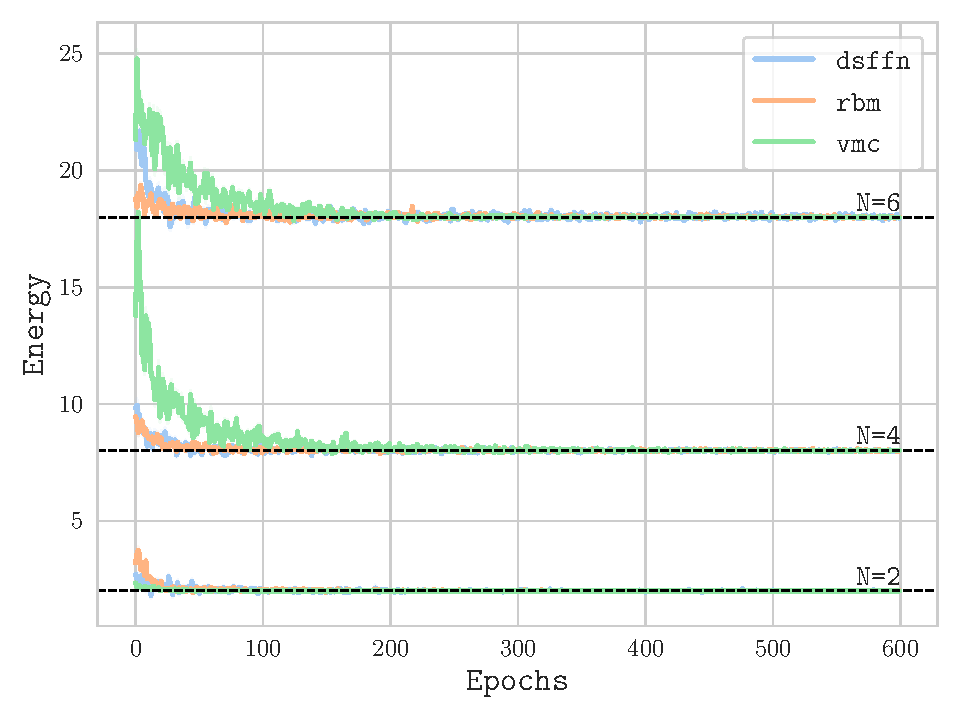
\includegraphics[width=0.55\linewidth]{Chapters/Results/N2/E_conv_ferm_pol_NI.pdf}
    \caption{Energy convergence curve for the non-interactive one-dimensional fully polarised fermionic system. In black dotted line, the analytical ground-state energies are marked. The models are Deep Set feed-forward network (DSFFN), restricted Boltzmann machine (RBM) and a standard variational Monte Carlo (VMC). Here we used Adam with learning rate of $0.01$ and Metropolis sampling.}
    \label{fig:E_conv_ferm_pol_NI}
\end{figure}

To check if reaching the ground-state energy results in an accurate wavefunction representation, one can generate a plot of the wavefunction. This is especially possible in the one-dimensional two-particle scenario, where the positions of each particle can be used as axes and the function value can be represented by a colorbar, as in \figref{fig:1D2P}. The values were obtained by uniformly sampling the positions for the particles and evaluating the output of a trained model, together with its sign. \figref{fig:1D2P} further serves to validate that despite working with $\ln|\psi|$ throughout the entire sampling and training process, we can recover the sign of the wavefunction. The profile shown is a classic fermionic representation, with a node region at $X_1 = X_2$ around which the wavefunction values are mirrored, except for a flip in sign. This is a consequence of the Pauli exclusion principle and the fact that we enforce the fermions to be polarised with the same spin.

\begin{figure}[H]
    \centering
    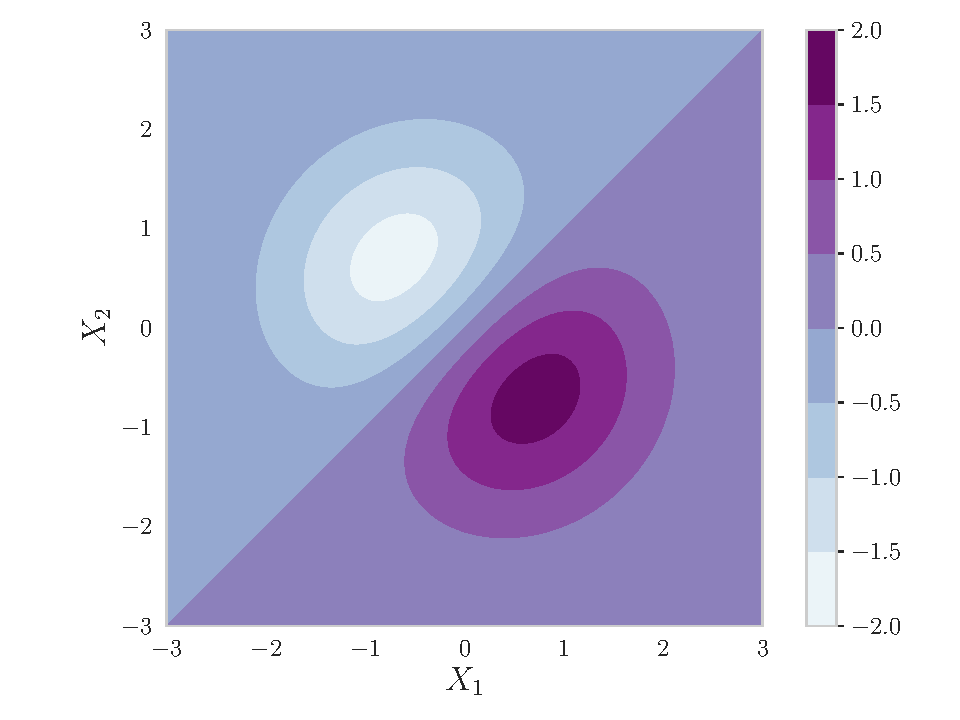
\includegraphics[width=0.7\linewidth]{Chapters/Results/N2/1D2P_wave_function.pdf}
    \caption{Two particle wavefunction for a one-dimensional fermionic ground-state. A clear fermionic nodal structure at $X_1 = X_2$ can be observed.}
    \label{fig:1D2P}
\end{figure}

We can compare the quality of our models and techniques without extensive parameter investigation for a small but interacting system of two particles ($N = 2$). At this stage, the results shown are merely investigations and are not fine-tuned in any way. In \figref{fig:N2_models_differentV0}, we compare our models with four values of interaction strength. We begin with an attractive regime of $V_0 = - 20$ and increase until we obtain a repulsive interaction $V_0 = 20$. In all interactive polarised fermionic systems, we limit ourselves to dealing with an interaction range of $\sigma_0 = 0.5$. The energy values displayed are a rolling average over ten epochs for better visuals. If, for example, 600 epochs were used, only 60 points make up the plot. 

Furthermore, \figref{fig:N2_models_differentV0} contains Hartree-Fock and CI energies, obtained with the code available from \cite{drissifermion}. It should be mentioned that the basis for the CI calculations was by no means a large one, with only 20 harmonic oscillator modes, and the Hartree-Fock calculations were obtained via $N$ integro-differential equations, where we iterate over the entire spatial grid computing the density and updating the Hamiltonian matrix at each step. Then, approximate eigenvalues are obtained via the Rayleigh-Ritz method.

All results shown in \figref{fig:N2_models_differentV0} used a block-diagonal approximation of the stochastic reconfiguration (SR) update rule with learning rate of $10^{-3}$. For all uses of this SR approximation, we also added a diagonal shift of $\lambda = 10^{-4}$ and a trust region for the update, described in \secref{sec:kfac}. The convergence curves have large deviations because small batch sizes were used. This means that only 500 MC proposals were sampled to collect the averages at each step. Consequently, the energy estimations fluctuate, and the gradient update, which is based on $\nabla \langle E_L\rangle$, also loses stability. 
\begin{figure}[H]
    \centering
    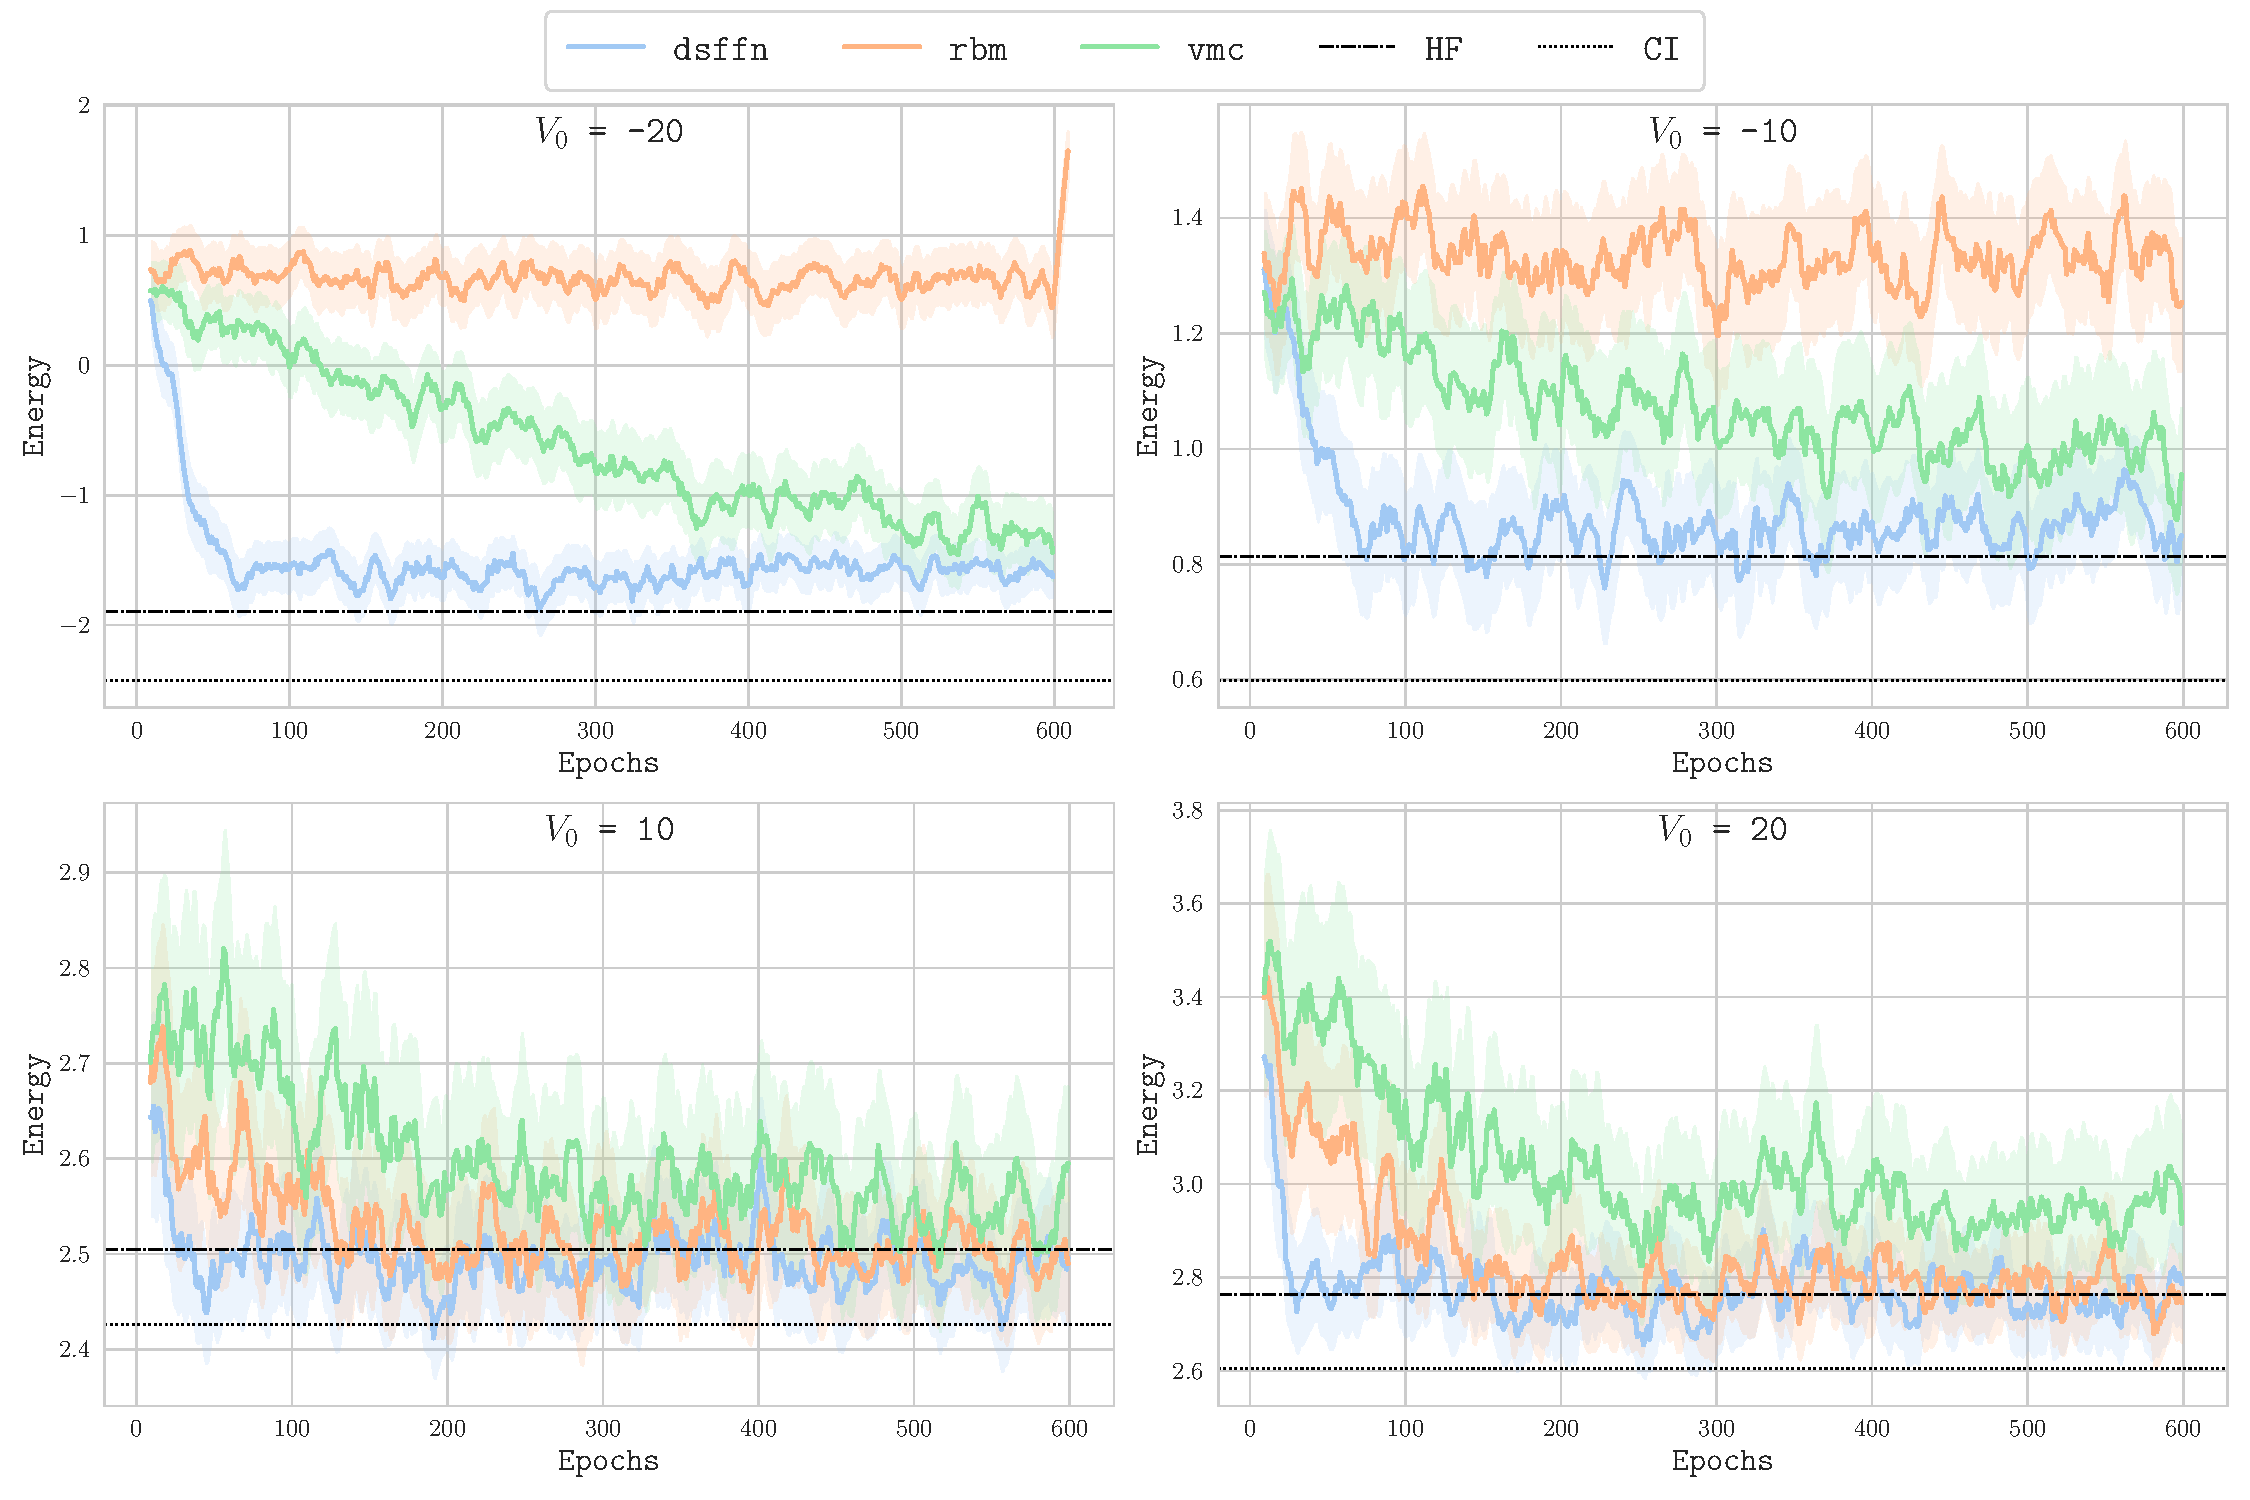
\includegraphics[width=1\linewidth]{Chapters/Results/N2/energy_convergence_v0_all.pdf}
    \caption{Energy convergence curve for the two particle ($N=2$) interactive problem of one-dimensional fully polarised fermions. The shaded area marks a $95\%$ confidence interval. In black dotted line, one can see Hartree-Fock and CI reference energies. None of the models used were fine-tuned, and the optimiser sheme was the stochastic reconfiguration method with a block-diagonal approximation.}
    \label{fig:N2_models_differentV0}
\end{figure}

Still with regard to \figref{fig:N2_models_differentV0}, the Deep Set model seems to outperform the other two, especially in the attractive regime. Although this could be attributed to a larger expressive power or more careful enforcement of \as, special mention must be credited to the pretraining stage. As detailed in \secref{sec:pretrain}, for feedforward networks, convergence for dimensions greater than one was only achieved by pre-training the ansatz in a supervised manner. Specifically, we fit the log probability of the ansatz to that of a multivariate Gaussian. It is known that in the attractive regime, the one-dimensional spinless fermions exhibit a density profile similar to non-interacting bosons \cite{valiente2020bose}, resulting in a density profile that closely resembles a Gaussian. This, together with a larger and expressive power and flexibility, can explain why the DSFFN performs better than the other models in the attractive regime.

\subsection{Correlation Factor}

A last analysis without extensive parameter experimentation can be seen in \figref{fig:jastrow}, where we select the deep set FFN ansatz of figure \figref{fig:N2_models_differentV0} for the same physical systems and compare convergence curves with and without the inclusion of the Jastrow factor. We see that, without the Jastrow factor, the model is capable of oscillating around the energy levels given by the Hartree-Fock calculations. Indeed, this variational ansatz uses a Gaussian envelope only with the determinant of Hermite polynomials, then approximating a single Slater determinant. Only with the introduction of the Jastrow factor can the energy values achieved go significantly lower than the HF approximation.

This observation is interesting. In principle, the universal approximation theorem guarantees that the neural network part of the ansatz can approximate any complex correlation factor which is not captured by the HF approximation. Although this might indeed be possible, the explicit addition of a correlation factor to the ansatz was what significantly enabled energies lower than HF. However, the statistics in \figref{fig:jastrow} are lacking, and we must examine the values and errors of larger Monte Carlo samples to be able to make this affirmation.

\begin{figure}[H]
    \centering
    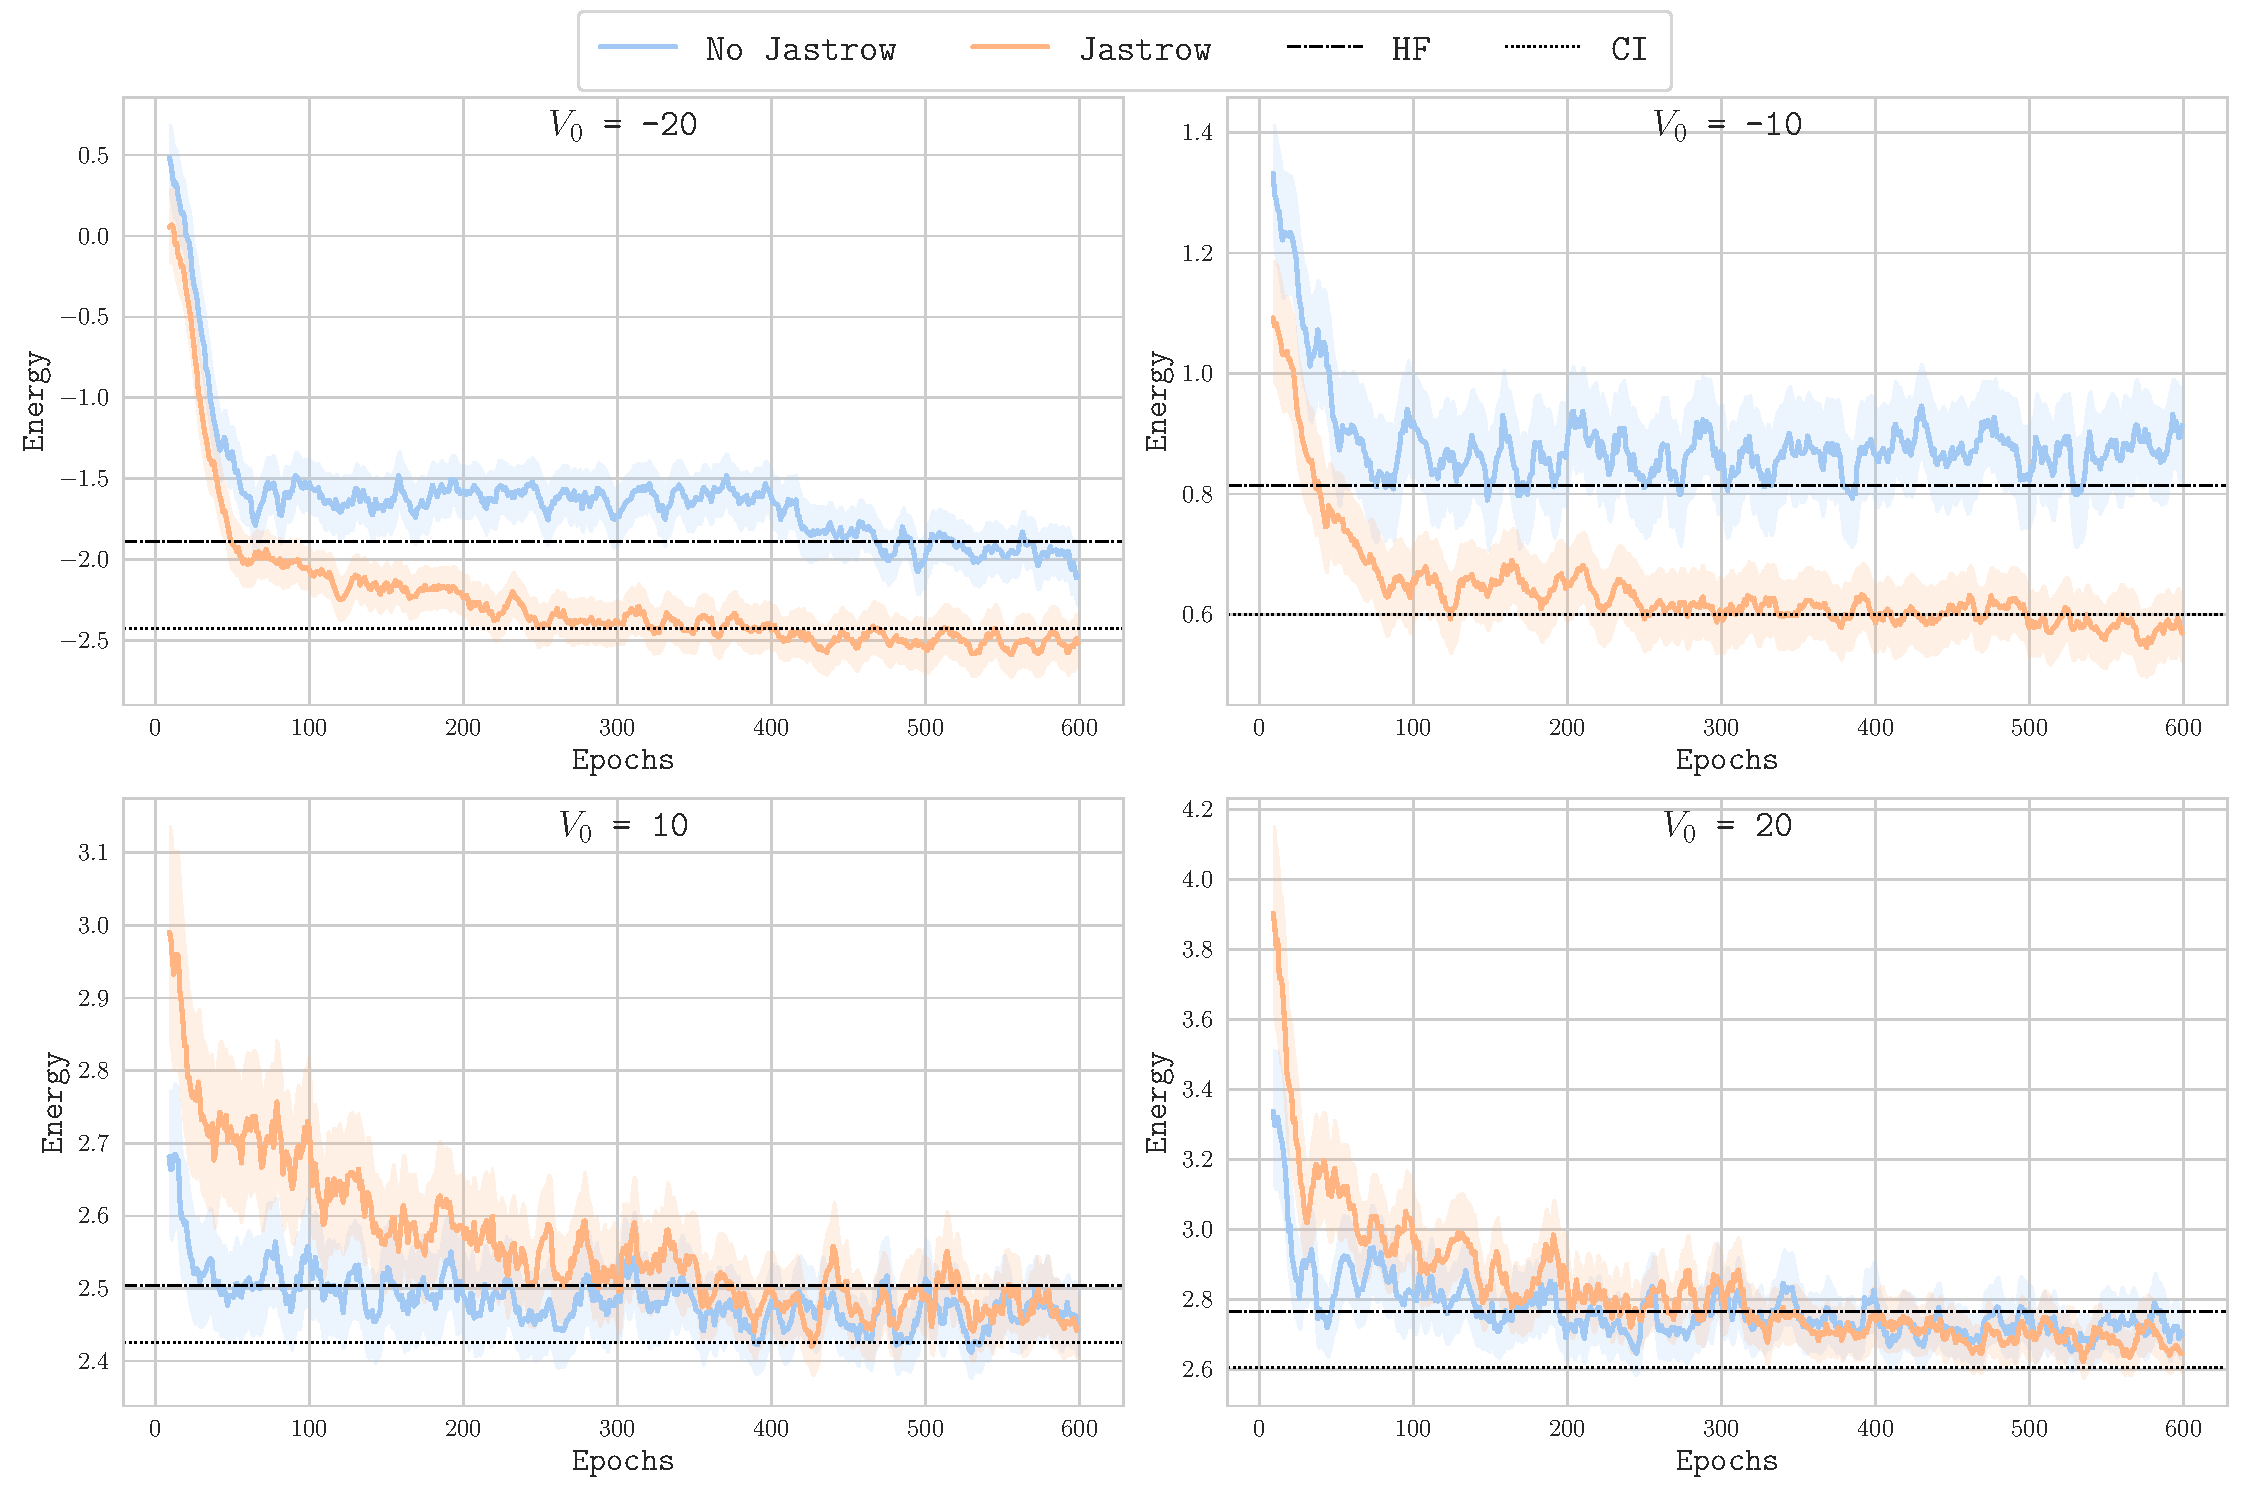
\includegraphics[width=1\linewidth]{Chapters/Results/N2/dsffnn_jastrow_energy_convergence_v0_all.pdf}
    \caption{Comparison between energy convergence curves for two particle ($N = 2$) for Deep Set feed-forward network with and without Jastrow factor. We an approximate stochastic reconfiguration optimiser, and the plot is displayer with a running average of 10 epochs. The shaded are represents a $95\%$ confidence interval.}
    \label{fig:jastrow}
\end{figure}

\section{Hyperparameter Search}\label{sec:sweep1d}

We then proceed to more thorough investigations via hyperparameter sweep searches. For each of our ansatz, we performed a sweep of approximately 300 configurations. This means that 300 sets of variational training were done, each with a random combination of options such as batch size, learning rate (here called ``Eta''), maximum training epochs, network architecture, and more. Figure \ref{fig:ds_complete_sweep} displays the sweep for the Deep Set ansatz, which involved 351 hyperparameter configurations. Analogous searches for VMC and RBM ansätze can be seen in the appendix \ref{apendix:more_results_1d}.

\begin{figure}[H]
    \centering
    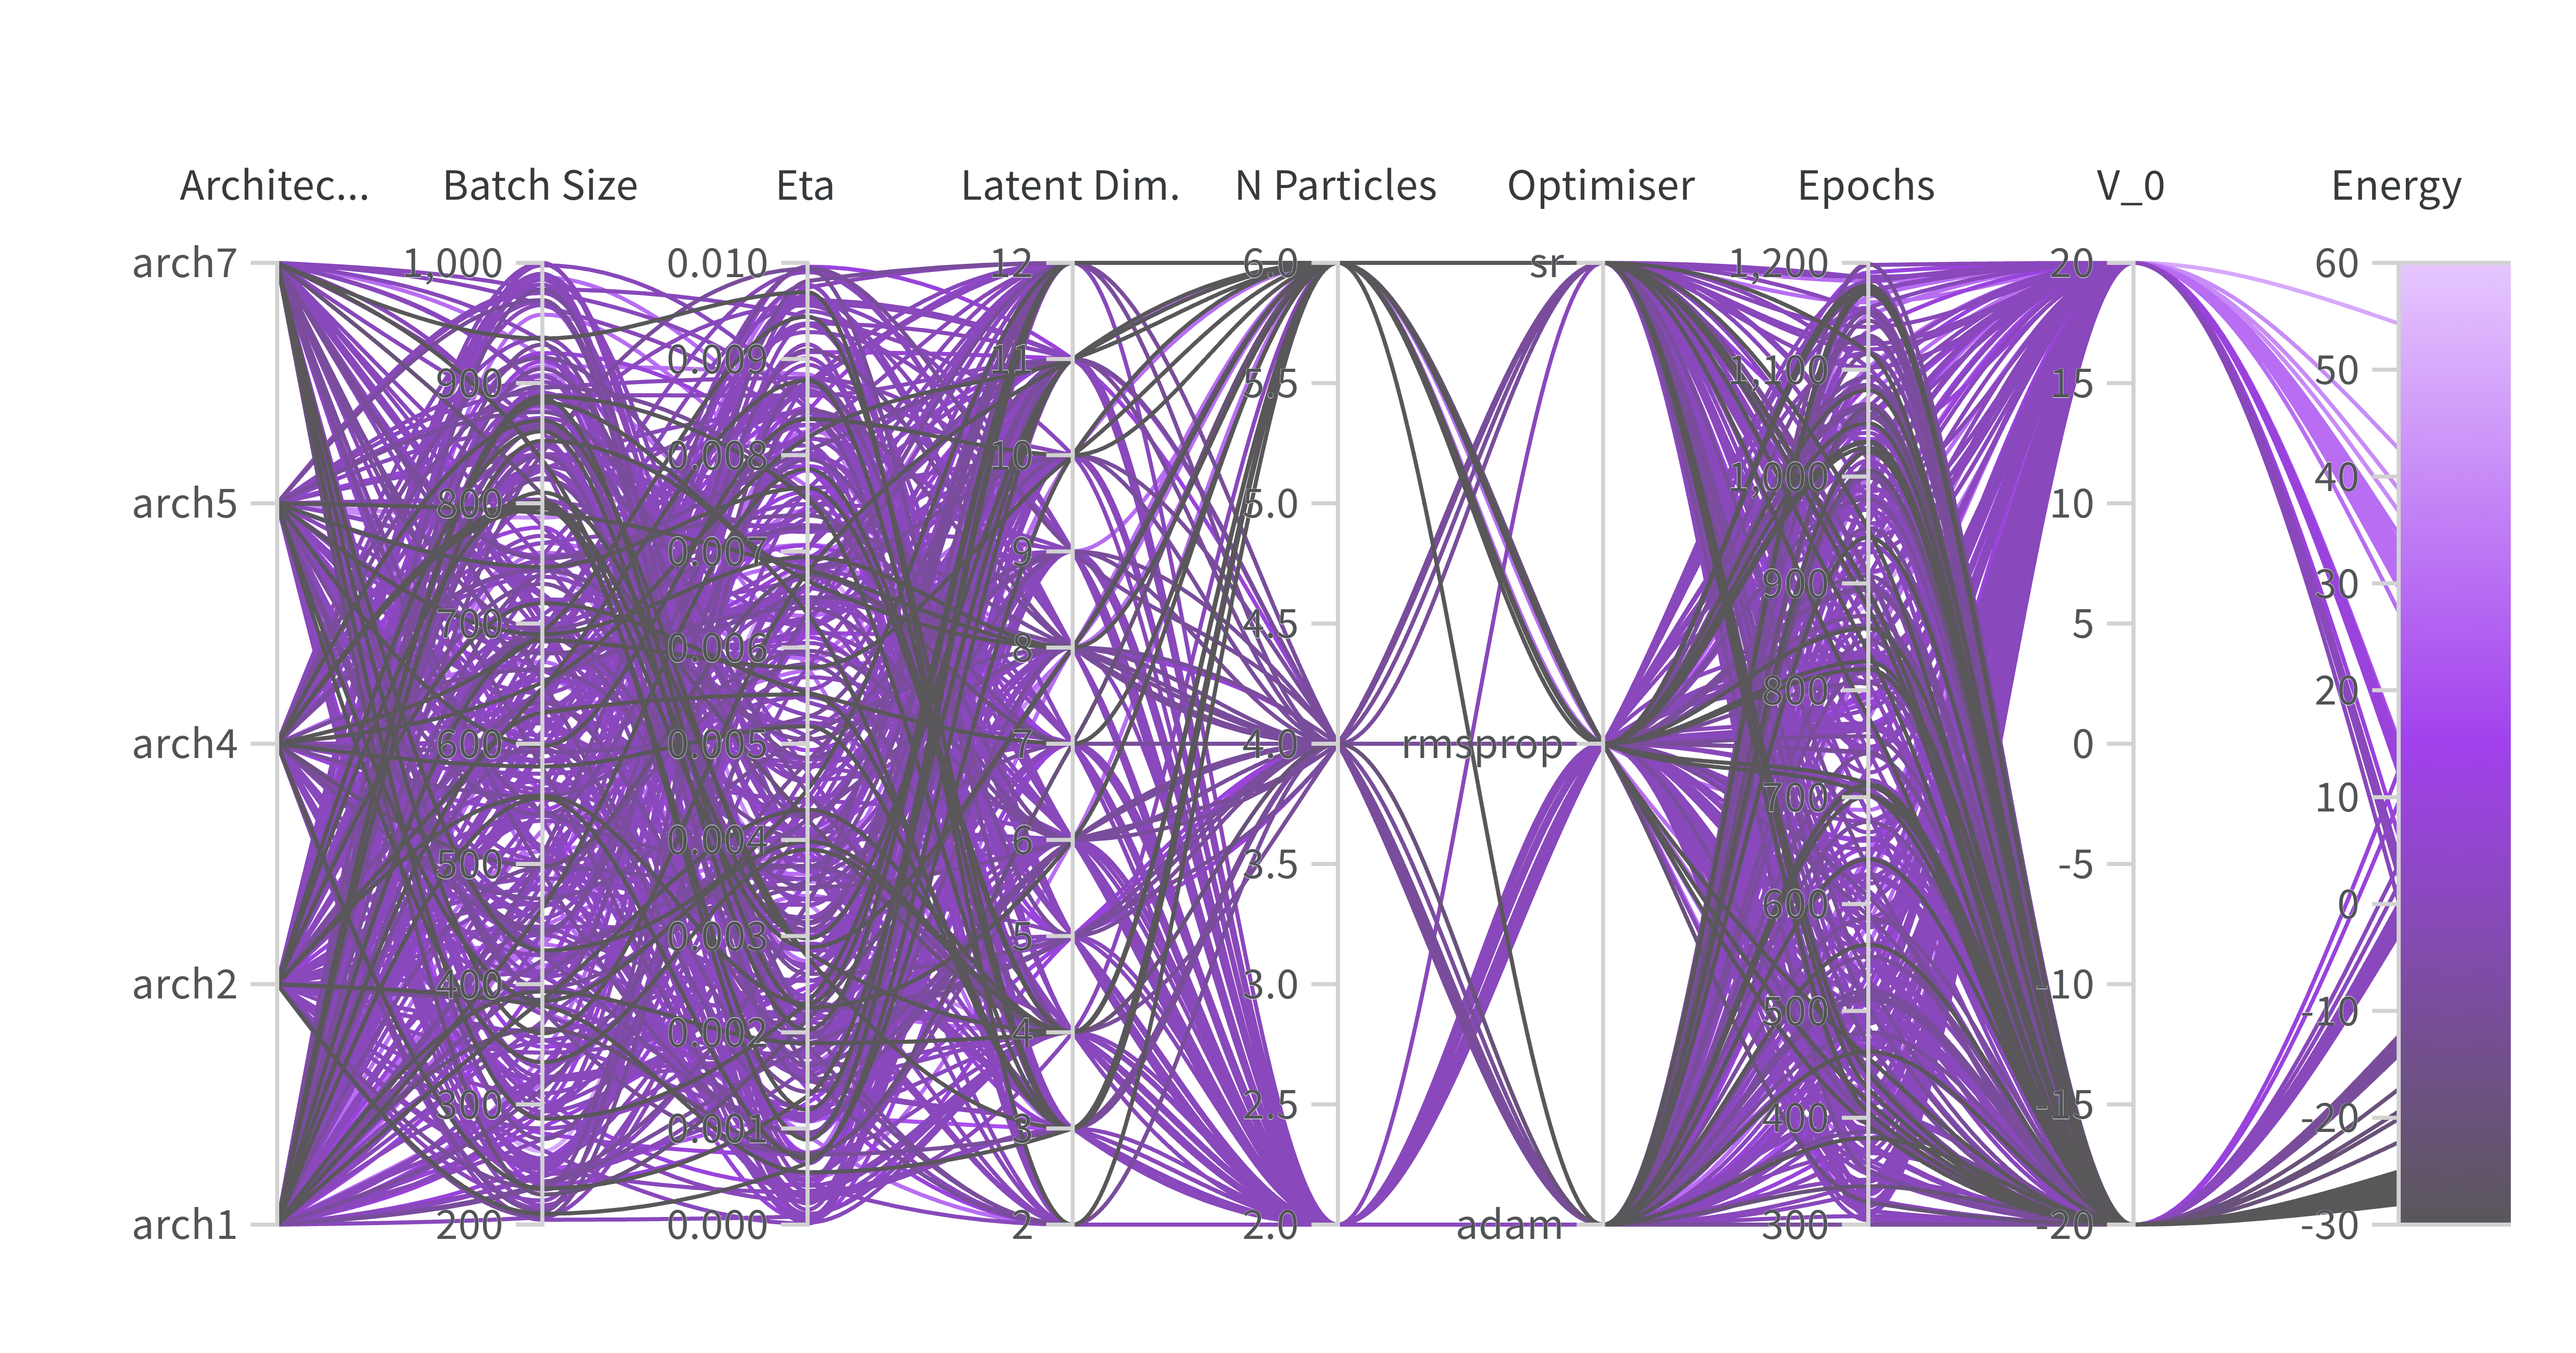
\includegraphics[width=0.8\linewidth]{Chapters/Results/N2/deepset_sweep.png}
    \caption{Sweep over 351 hyperparameters for the standard DSFNN ansatz, from which the results shall be aggregated from. Table \ref{tab:arch} displays the different architectures experimented, here simply marked as ``arch''.}
    \label{fig:ds_complete_sweep}
\end{figure}

\begin{table}[h!]
\centering
\caption{Deep Set architectures Overview for sweep, for the sweep performed in \figref{fig:ds_complete_sweep}. The values missing in the architecture order were discarded for frequent non-convergence behaviour. The latend dimension $L_d$ is chosen independently.}
\label{tab:arch}
\begin{tabular}{@{}lccccc@{}}
\toprule
\textbf{Architecture Nr.} & \multicolumn{2}{c}{\textbf{Activations}} & \multicolumn{3}{c}{\textbf{Layer Sizes}} \\ 
\cmidrule(lr){2-3} \cmidrule(lr){4-6}
 & $\phi$ & $\rho$ & $\phi$ & Pooling & $\rho$ \\ 
\midrule
\textbf{1} & GELU $\times$ 4 & GELU, linear & 7, 5, 3, $L_d$ & Avg & $L_d$, 3, 1 \\ 
\textbf{2} & GELU $\times$ 5 & GELU $\times$ 3, linear & 10, 7, 5, 3, $L_d$ & Avg & $L_d$, 6, 4, 2, 1 \\ 
\textbf{4} & GELU $\times$ 5 & GELU $\times$ 2, linear & 9, 7, 5, 3, $L_d$ & Avg & $L_d$, 5, 3, 1 \\ 
\textbf{5} & GELU $\times$ 5 & GELU $\times$ 2, linear & 14, 9, 7, 5, $L_d$ & Avg & $L_d$, 5, 3, 1 \\ 
\textbf{7} & GELU $\times$ 5 & GELU $\times$ 2, linear & 12, 9, 7, 5, $L_d$ & Avg & $L_d$, 6, 4, 1 \\ 
\bottomrule
\end{tabular}
\end{table}


\subsection{Optimisers}
From the sweep of \figref{fig:ds_complete_sweep}, several results can be aggregated and averages can be taken for certain configurations. For instance, \figref{fig:N2V0=-20_OPT} isolates the case where the interaction strength is $V_0$ and, for a different number of particles, extracts the average energy values for the different choices of optimisers. The figure suggests that among the optimisers evaluated, the stochastic reconfiguration variant consistently outperformed the others, significantly contributing to a lower average value across more than 300 different parameter settings and different number of particles. Although we show only attractive interactions of $V_0 = -20$, the same was observed for repulsive interactions. This motivated the choice of the SR optimiser for all the following results. AdaGrad was consistently the worst optimiser tested, at least for the parameters used.

\begin{figure}[H]
    \centering
    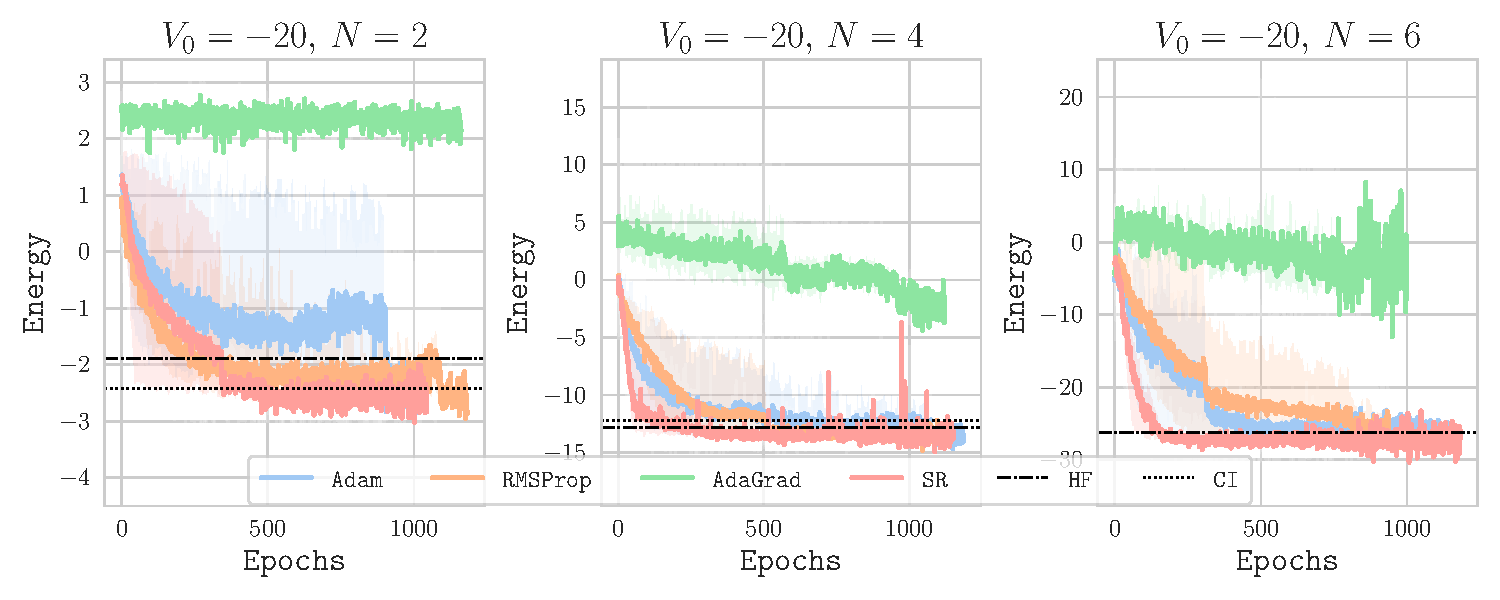
\includegraphics[width=1\linewidth]{Chapters/Results/N2/opti_sweepv0-20.pdf}
    \caption{Training energy averages and standard deviations for the aggregated values of the hyperparameter search of \figref{fig:N2V0=-20_OPT}. Results are displayed for two, four and six particles with interaction $V_0=-20$. Here, the shaded are is not the confidence interval, but the minimum and maximum observed in the parameter search.}
    \label{fig:N2V0=-20_OPT}
\end{figure}

\subsection{Importance sampling}

Another choice that can be investigated from \ref{fig:ds_complete_sweep} is how the expected energy value is affected by the use of importance sampling, discussed in \secref{sec:langevin_imporance}. Figure \ref{fig:comparison_sampling} compares this for different number of particles and the extreme or the interaction strengths, both attractive and repulsive.

\begin{figure}[H]
    \centering
    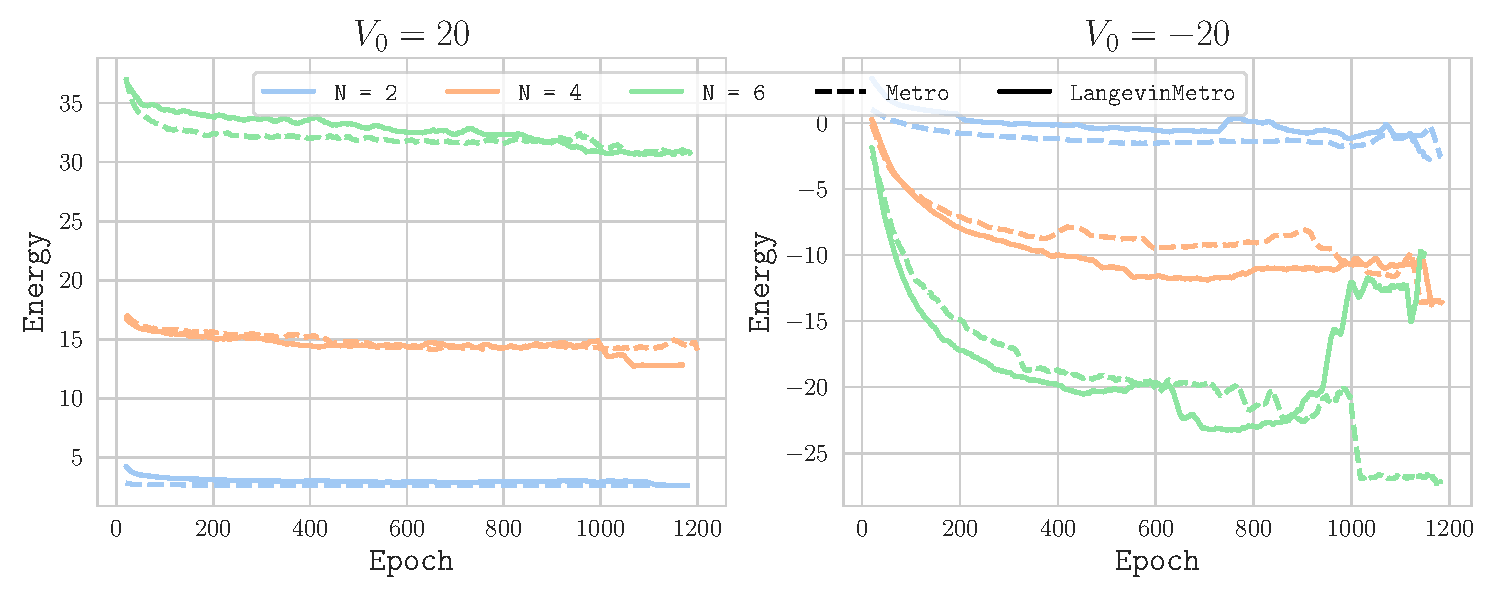
\includegraphics[width=0.9\linewidth]{Chapters/Results/N2/lmh_vs_m.pdf}
    \caption{Comparison of the averaged values over all 321 runs of the sweep shown in figure \figref{fig:ds_complete_sweep} aggregated by number of partciles, interaction stren, rolling window of 20. Errorbars are not included. Here, ``LagevinMetro'' depicts importance sampling.}
    \label{fig:comparison_sampling}
\end{figure}

There is a notable gap regarding whether the choice of importance sampling will, on average, produce better results, as illustrated in \figref{fig:comparison_sampling}. This gap seems to depend on the character of the interaction, where the attractive regime favoured importance sampling over the regular Metropolis algorithm. Although it is challenging to speculate on the exact cause, one potential explanation is the width of the distribution we aim to approximate. In the attractive regime, the distribution tends to be more localised, making standard sampling techniques less efficient. Consequently, for broader distributions, various sampling methods might perform equally well. However, when greater efficiency is needed, importance sampling proved to be more effective.

\begin{figure}[H]
    \centering
    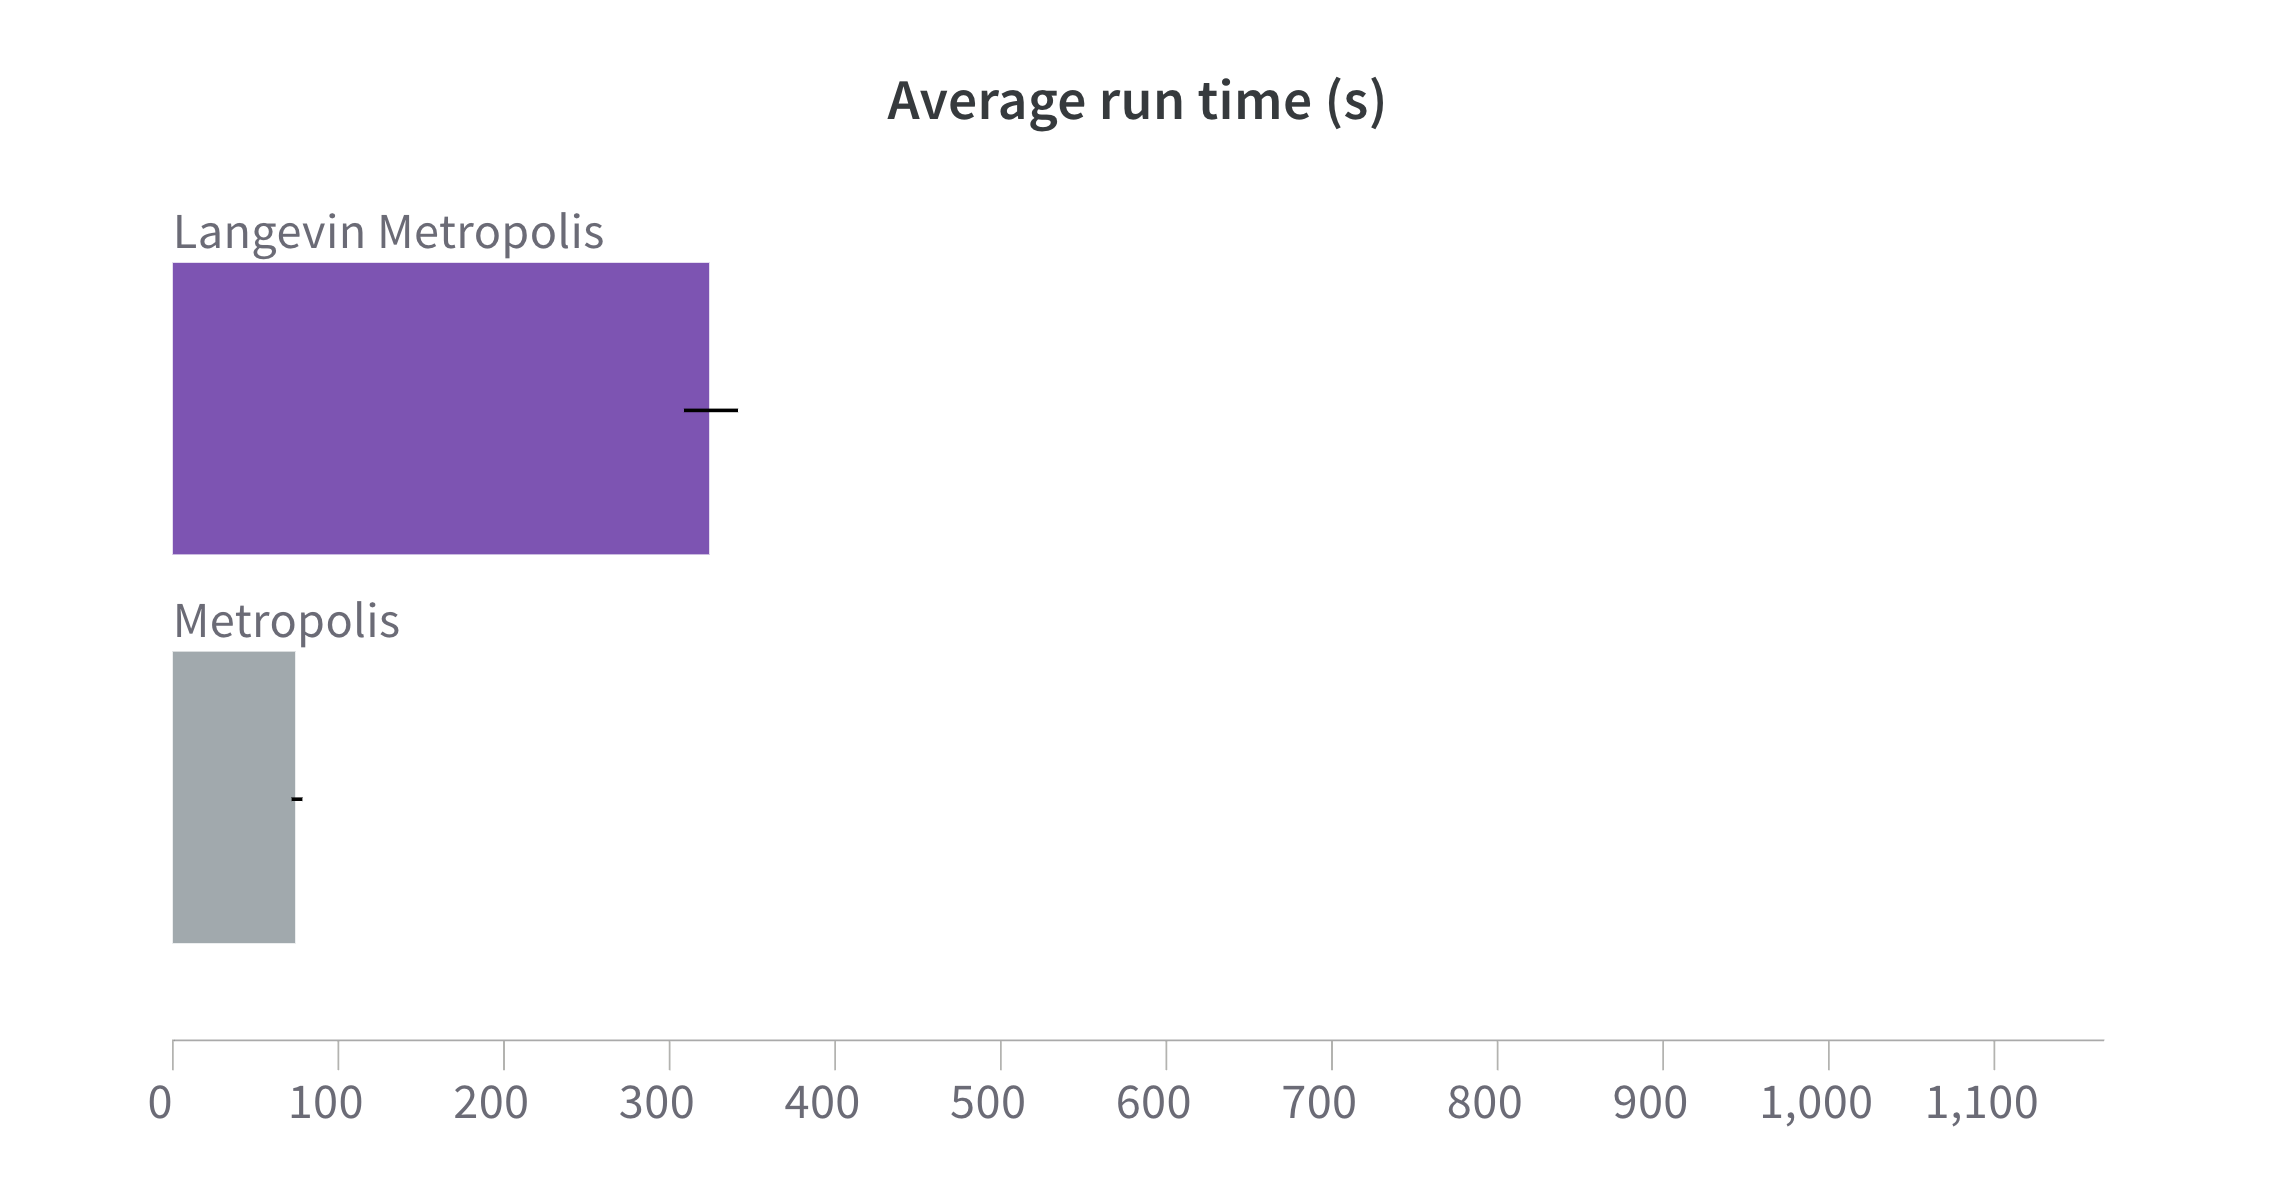
\includegraphics[width=0.7\linewidth]{Chapters/Results/N2/avg_run_time_lm_m.png}
    \caption{Average runtime comparison of the Langevin Metropolis (importance sampling) and the regular Metropolis Makov chain Monte Carlo over 321 randomised runs. The line in black depicts the standard error of the mean.}
    \label{fig:time_metro_langevin}
\end{figure}

Despite the importance sampling technique displaying some advantage over a regular Metropolis Sampling, time complexity must be taken into account. On that note, \figref{fig:time_metro_langevin} shows the average run-time for all configurations displayed in \figref{fig:ds_complete_sweep}. Not all averages include the same batch size or number of training epochs; however, these seem to be equally distributed between sampler options. Figure \ref{fig:ds_complete_sweep} motivates us not to use importance sampling as a method throughout the remainder of this study. There is approximately a threefold discrepancy between average runtimes, and the difference in minimised energy value did not seem to justify its use. The small difference in energy is further supported by \cite{Nordhagen2019}. Although importance sampling has been shown to be necessary for the use of diffusion Monte Carlo \cite{kalos1974helium}, its benefits may not be as significant for VMC.

What explains at least part of the discrepancy in computational time is the need to calculate the drift force, $F = 2\nabla\ln|\psi|$, and the ratio of Green's functions, as displayed in \eqref{eq:met:metric_metropolis_hastings} and \eqref{eq:acceptance_langevin_metro_def}. Although this alone should not have an effect as large as observed, one specific point must be mentioned. For implementation reasons, and to make the Langevin-Metropolis method general to all ansätze, the calculation of the drift force required reshape manipulation of the input position vector. We tried to mitigate this, with no success. As mentioned in \ref{sec:jax}, JAX arrays are supposed to be static, so we strongly believe that a big part of the difference in computational time is due to JAX not being able to fully pre-compile this calculation.

\section{Energy Components}

Now, instead of displaying the average results in a series of configurations, we selected parameters based on the ranges that gave good results from the hyperparameter search of \secref{sec:sweep1d}. For the results that follow, some common choices were made. All results displayed hereafter were performed with trial functions that included a Jastrow factor, and the optimiser of choice was always stochastic reconfiguration. These calculations involve longer training processes and more extensive sampling.

More specifically, \figref{fig:energy_components1d} shows the distribution of the energy components as a function of the interaction strength for all ansätze and different numbers of particles. The different trial functions agreed reasonably well in terms of energy values, and a better comparison can be seen in Table \ref{tab:energy_components1d}.

The energy curves in \figref{fig:energy_components1d} are expected, showing that the energy scale varies with the particle count, while the ratios between the energy components mirror the findings of \cite{drissifermion}, from which we extract some analysis.

First, the total energy $E$ increases when going from an attractive to a repulsive regime. The potential energy increases with the strength of the interaction, but the apparent plateau, together with a decrease in kinetic energy, indicates fermion localisation. This point will be discussed in the analysis of the density profiles. 

When the interaction is extremely attractive, the particles are concentrated in the centre of the trap. In this scenario, the absolute magnitude of the interaction surpasses that of the kinetic energy, and there is almost a cancelation of the trap potential. As also achieved by \cite{drissifermion}, in some instances we observe $\langle K \rangle \leq \langle V_{int} \rangle$, which is a sign of Wigner crystallisation \cite{Vu_2020}.

\begin{figure}[H]
    \centering
        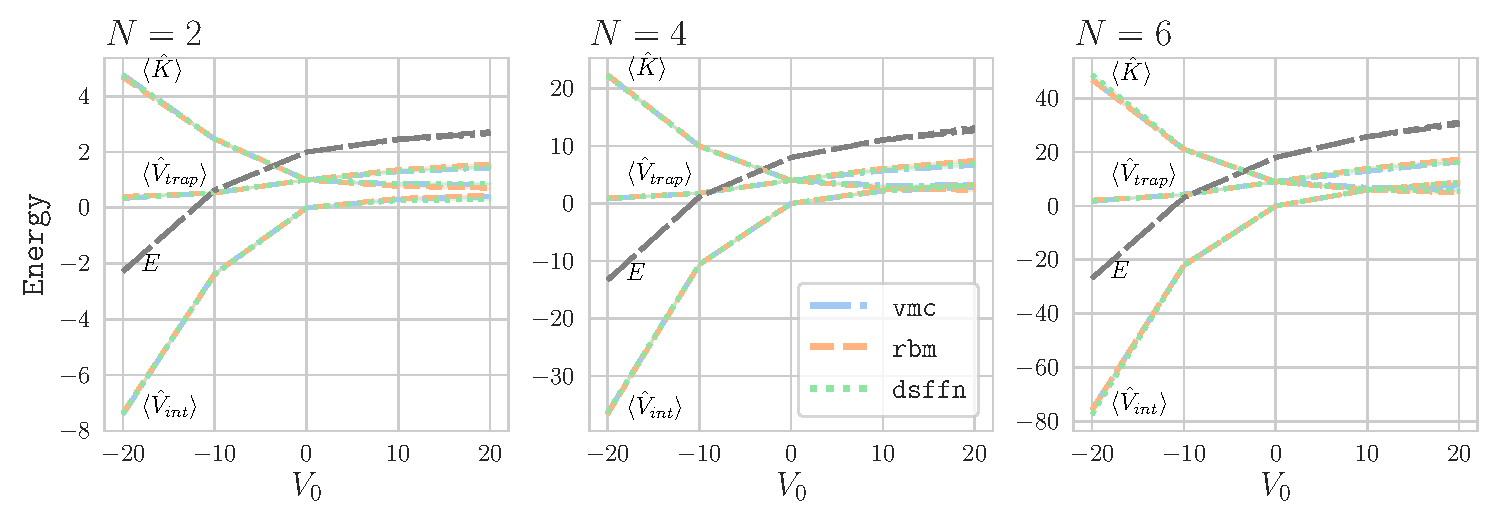
\includegraphics[width=1\linewidth]{Chapters/Results/N2/energy_components_vs_v0.pdf}
    \caption{Energy components as a function of the interaction strength, $V_0$, for different number of particles and trial wavefunctions. All wavefunctions were multiplied by a Jastrow factor. The values were obtained with after $10^{24}$ Monte Carlo samples, SR optimiser and 1500 epochs of training.}
    \label{fig:energy_components1d}
\end{figure}

In Table \ref{tab:energy_components1d} we also show the ratio between kinetic energy and the sum of potential energies for a four-particle system. As dictated by the virial theorem, in the non-interacting case, $\langle E\rangle = 2\langle \hat{K}\rangle = 2\langle \hat{V}_{trap}\rangle$. This is verified with the fraction of the kinetic and potential energies resulting in 1. Again, we note an acceptable yet not perfect agreement between the different models.

\begin{table}[H]
    \centering
\begin{tabular}{c|c|c|c|c|c|c}
\toprule
\multirow{2}{*}{\textbf{Ansatz}} & \multirow{2}{*}{$V_0$} & \multirow{2}{*}{$E$} & \multirow{2}{*}{$\langle \hat{K}\rangle$} & \multirow{2}{*}{$\langle \hat{V}_{trap}\rangle$} & \multirow{2}{*}{$\langle \hat{V}_{int}\rangle$} & \multirow{2}{*}{$\frac{\langle \hat{K} \rangle}{\langle \hat{V}_{trap} \rangle + \langle \hat{V}_{int} \rangle}$} \\
 & & & & & & \\
\midrule
\multirow{5}{*}{DSFFN + SJ}& -20& -13.372(3) & 22.16(1) & 0.8303(5) & -36.364(9) & -0.624
\\
 & -10& 1.1421(9) & 9.941(5) & 1.797(1) & -10.595(4) & -1.130 \\
 & 0& 8.00028(6) & 4.000(2) & 4.000(2) & 0(0) & 1.000 \\
 & 10& 11.009(1) & 2.906(2) & 5.921(2) & 2.182(2) & 0.357 \\
 & 20& 13.244(8) & 3.021(8) & 6.998(3) & 3.224(3) & 0.296 \\
\midrule
\multirow{5}{*}{RBM + SJ} & -20& -13.294(3) & 22.36(1) & 0.9751(8) & -36.63(1) & -0.627 \\
 & -10& 1.145(1) & 9.983(5) & 1.772(1) & -10.610(4) & -1.13 \\
 & 0& 8.00123(8) & 3.998(2) & 4.004(2) & 0(0) & 0.999 \\
 & 10& 11.101(1) & 2.684(1) & 6.089(3) & 2.328(2) & 0.319 \\
 & 20& 13.025(2) & 2.271(1) & 7.476(3) & 3.278(3) & 0.211 \\
\midrule
\multirow{5}{*}{VMC + SJ}& -20 & -13.360(3) & 22.261(9) & 0.8186(4) & -36.439(9) & -0.625 \\
 & -10& 1.1452(9) & 9.978(5) & 1.781(1) & -10.614(4) & -1.130 \\
 & 0& 8.000028(4) & 3.998(2) & 4.002(2) & 0(0) & 0.999 \\
 & 10& 11.0009(7) & 3.161(2) & 5.674(2) & 2.166(2) & 0.403 \\
 & 20& 12.650(1) & 3.222(2) & 6.647(2) & 2.781(3) & 0.321 \\
\bottomrule
\end{tabular}
\caption{A more detailed display of the energy components of \figref{fig:energy_components1d}, for four particles.}
\label{tab:energy_components1d}
\end{table}


\section{One-body Densities}

In terms of one-body density profile, \figref{fig:density_n2} shows in isolation the two-particle case for all ansätze and different interactions, and \figref{fig:densities_all} shows the other cases, up to six particles. From these figures, it becomes clear that, for both an attractive regime and a larger number of particles, getting the models to agree becomes challenging. However, even when the methods disagree, some qualitative points can be addressed. Even for a different number of particles, once the interaction strength is set, the width of the distribution remains the same. Furthermore, the peak of the distributions becomes taller with an increase in the number of particles as $n(\mathbf{x})$ must integrate to $N$, but with the system constrained by the trap.

Importantly, as analysed in terms of energy components, the attractive regime demonstrates a peak at the centre of the trap, in a process corresponding to the bosonization of polarised fermions \cite{valiente2020bose}. On the other extreme, the repulsive interaction results in clear peaks or fringes. The number of peaks corresponds to the number of particles in the system and should, in principle, be symmetric around the origin. 

\begin{figure}[H]
    \centering
    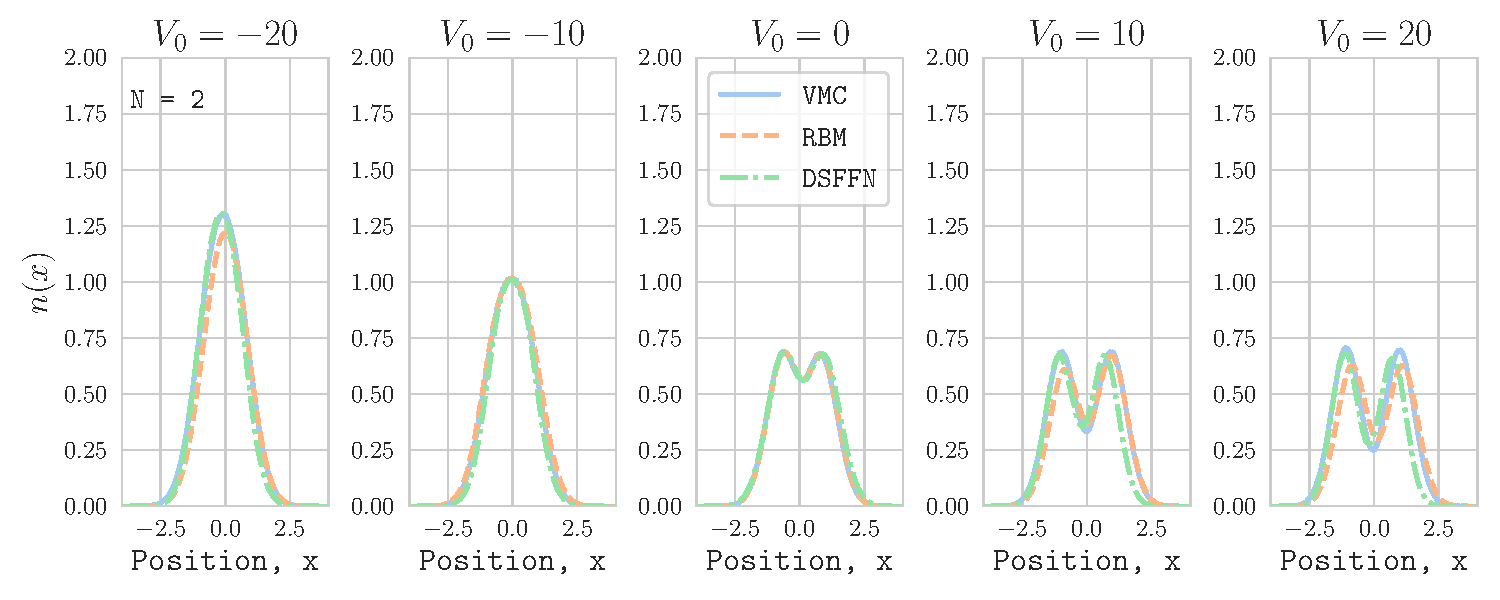
\includegraphics[width=1\linewidth]{Chapters/Results/N2/density_profile_N[2]_nqs_DSFFN.pdf}
    \caption{Density profiles $n(x)$ for two particles at different interaction strengths and for different trial functions, all accompanied by a Jastrow factor. The profile was based on $2^{24}$ samples, with average energies displayed in Tab. \ref{tab:final_energies}}
    \label{fig:density_n2}
\end{figure}

As shown in \figref{fig:densities_all}, the peaks become more pronounced with a stronger interaction, although not all models follow the symmetry constraint well. The VMC function appears to perform the best in this regard. Conversely, the RBM shows significant asymmetry with stronger repulsive interactions and fails to capture the fringes for three interaction strengths in the two-particle scenario. We will explore how this relates to the energy value in \secref{sec:energy}, but we can already discuss this behaviour with respect to the symmetry of the ansätze.

Both mathematically and due to the trap symmetry, the probability density of the antisymmetric wavefunction should be symmetric. Although this seems to be approximately the case in \figref{fig:densities_all} it is certainly not true for all the examples shown. One cause, apart from us not being in the true ground-state, is that the initial ansatz does not perfectly adhere to any symmetry. Due to the potential variations in weights and biases for different particle inputs, the RBM, the VMC Gaussian ansatz, or the Jastrow factor are not ideally symmetric. For instance, even when the Deep Set ensures symmetry and is combined with a determinant that is inherently antisymmetric, the Jastrow factor has the potential to negate this symmetry. We expected this behaviour to be not as dramatic for the Deep Set, but it seems like the VMC was the best in that regard.

\begin{figure}[H]
    \centering
    \begin{subfigure}[b]{0.8\textwidth}
        \centering
        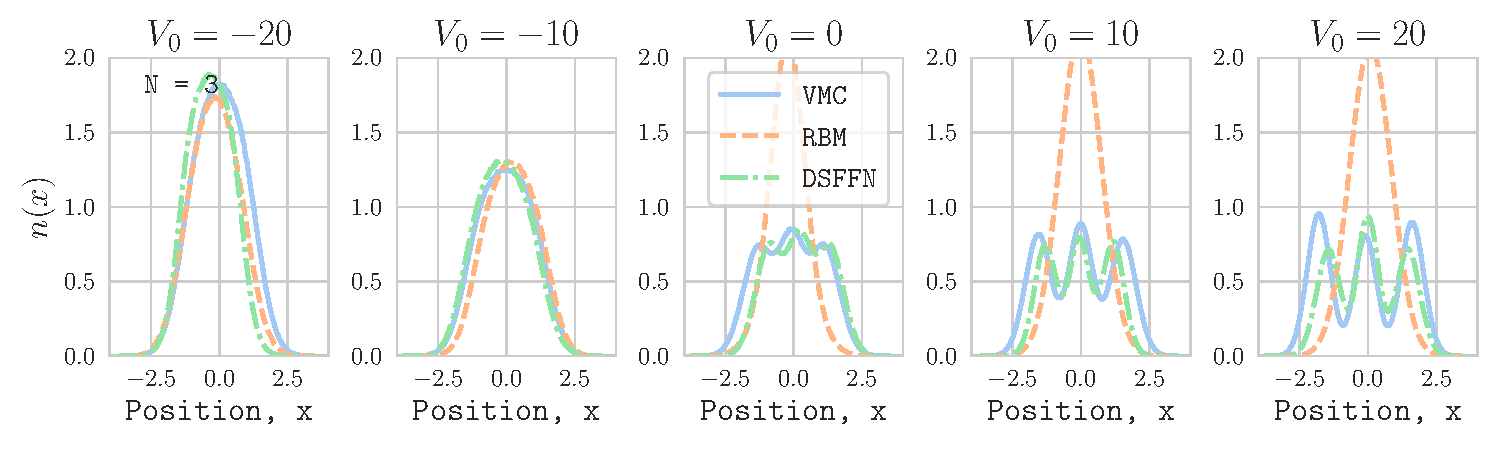
\includegraphics[width=\textwidth]{Chapters/Results/N2/density_profile_N[3]_nqs_DSFFN.pdf}
        \label{fig:total_n2}
        \vspace{-1.25cm}
    \end{subfigure}
    \begin{subfigure}[b]{0.8\textwidth}
        \centering
        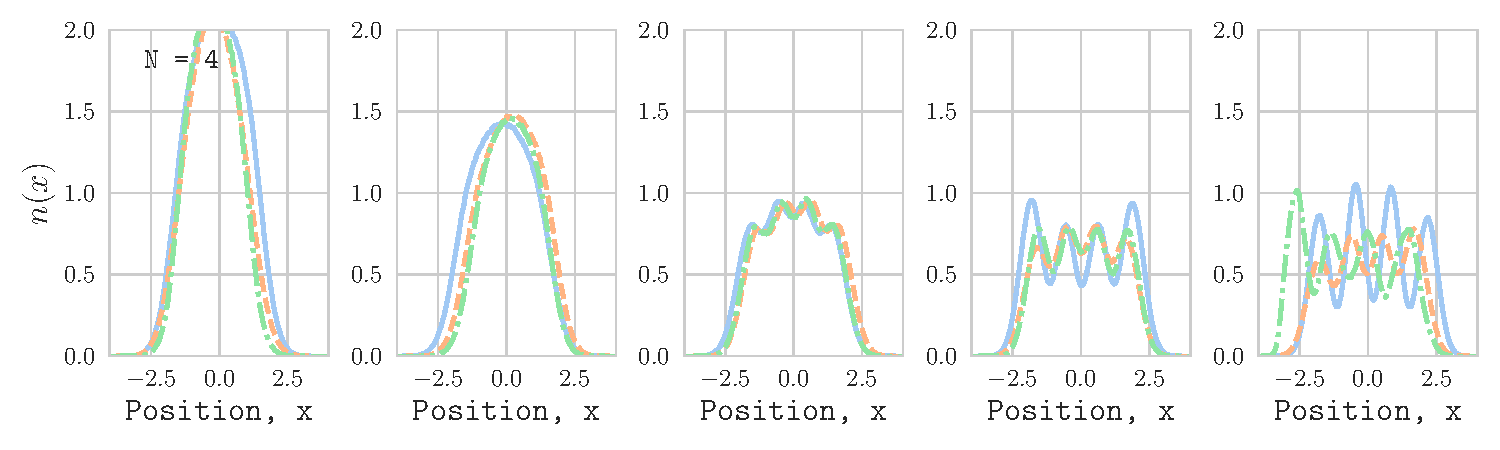
\includegraphics[width=\textwidth]{Chapters/Results/N2/density_profile_N[4]_nqs_DSFFN.pdf}
        \label{fig:total_n4}
        \vspace{-1.25cm}
    \end{subfigure}
    \begin{subfigure}[b]{0.8\textwidth}
        \centering
        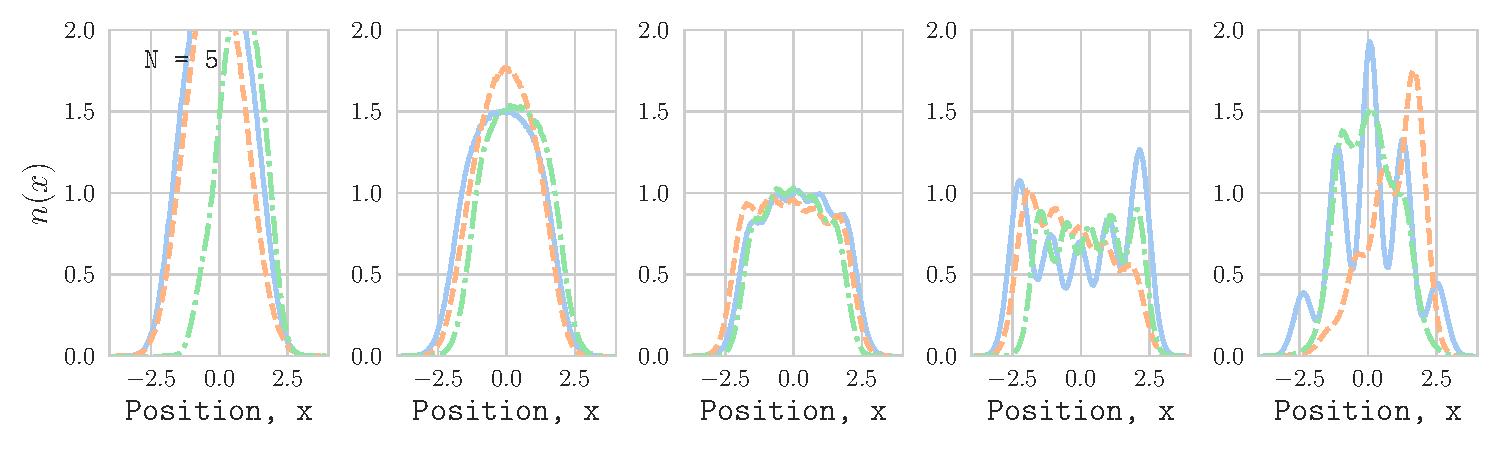
\includegraphics[width=\textwidth]{Chapters/Results/N2/density_profile_N[5]_nqs_DSFFN.pdf}
        \label{fig:total_n6}
        \vspace{-1.25cm}
    \end{subfigure}
    \begin{subfigure}[b]{0.8\textwidth}
    \centering
    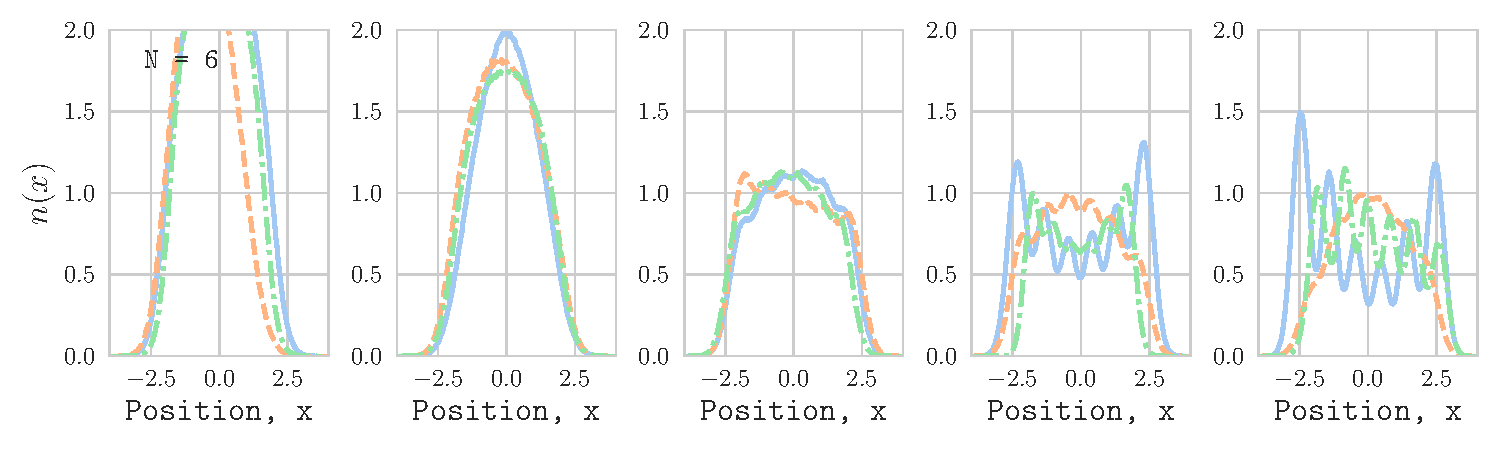
\includegraphics[width=\textwidth]{Chapters/Results/N2/density_profile_N[6]_nqs_DSFFN.pdf}
    \label{fig:total_n6}
    \end{subfigure}
    \caption{Density profiles for different ansätze, after $2^{24}$ MC samples. All ansatze were multiplied by a Jastrow factor, and the sampled energies can be found in Tab. \ref{tab:final_energies}}
    \label{fig:densities_all}
\end{figure}


\section{Overall Energy Comparison}\label{sec:energy}

Figure \ref{fig:corrlation_e} shows that regardless of the model, the energy obtained is lower than the Hartree-Fock energy for every interaction $V_0$. While this figure shows only a two, four and six-particle case, Tab. \ref{tab:final_energies} reveals that this is equally true for other cases. Moreover, there is a clear ease in energy minimisation for the attractive regime. Apart from that, to gauge which models yield the lowest average energy, we can look at the average energy value over all particles and interactions.

\begin{figure}[H]
    \centering
    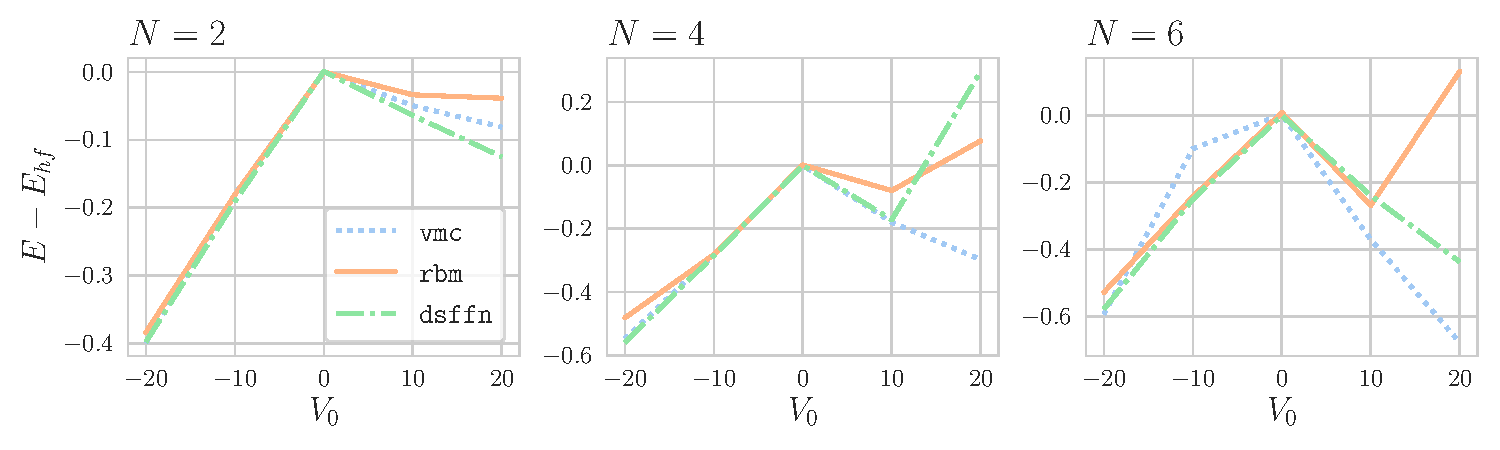
\includegraphics[width=\textwidth]{Chapters/Results/N2//total_energy_vs_v0_n6.pdf}
    \caption{Difference between the energy sampled and the HF energy versus interaction strength $V_0$. Error bars are included but too small to see. For a complete overview of the energies for other number of particles, \ref{tab:final_energies}. All values are result of $10^{24}$ samples after $1500$ epochs of training with Jastrow factor included.}
    \label{fig:corrlation_e}
\end{figure}

We further notice that there is a clear correlation between the lowest energy values obtained in Tab. \ref{tab:final_energies} and a density profile that is closer to what is expected in \ref{fig:densities_all}. For instance, the RBM failed to replicate the expected fringes for three particles in the repulsive interaction. Then, even though the density profile was symmetrical, resembling a Gaussian shape, we see that the energy values for the other two models were lower in that regime. Furthermore, both the RBM and DSFFN model displayed some asymmetry in the five-particle attractive regime, and that is reflected in a significantly higher energy value in comparison to the VMC.

\begin{table}[h]
\centering
\begin{tabular}{c|c|c|c|c|c|c}
\toprule
\textbf{N} & $V_0$& \textbf{DSFFN + SJ} & \textbf{RBM + SJ} & \textbf{VMC + SJ} & \textbf{HF} \cite{drissifermion} & \textbf{CI} \cite{drissifermion} \\
\midrule
\multirow{5}{*}{2} & -20 & -2.289(1) & -2.275(2) & -2.290(1) & -1.891464 & -2.4246 \\
& -10 & 0.6230(5) & 0.6329(6) & 0.6334(6) & 0.813691 & 0.5991 \\
& 0 & 2.00082(5) & 2.000023(7) & 2.0000000(7) & 2.000000 &  \\
& 10 & 2.4401(2) & 2.4705(4) & 2.4545(3) & 2.504193 & 2.4256 \\
& 20 & 2.6396(3) & 2.7258(7) & 2.6832(5) & 2.764479 & 2.6057 \\
\midrule
\multirow{5}{*}{3} & -20 & -7.172(2) & -6.51(2) & -7.249(2) & -6.764263 & -7.0593 \\
& -10 & 0.7709(8) & 1.014(8) & 0.7645(7) & 1.016808 & 0.7300 \\
& 0 & 4.50211(8) & 4.589(2) & 4.500016(6) & 4.500000 &  \\
& 10 & 5.9627(6) & 6.020(1) & 5.9533(4) & 6.061344 & 5.8781 \\
& 20 & 6.760(1) & 6.883(2) & 6.7106(7) & 6.887364 & 6.5153 \\
\midrule
\multirow{5}{*}{4} & 20 & 13.244(8) & 13.025(2) & 12.650(1) & 12.947469 & 12.3408 \\
& 10 & 11.009(1) & 11.101(1) & 11.0009(7) & 11.180564 & 10.8916 \\
& 0 & 8.00028(6) & 8.00123(8) & 8.000028(4) & 8.000001 &  \\
& -10 & 1.1421(9) & 1.145(1) & 1.1452(9) & 1.426522 & 1.1113 \\
& -20 & -13.372(3) & -13.294(3) & -13.360(3) & -12.812753 & -12.1935 \\
\midrule
\multirow{5}{*}{5} & -20 & -19.633(4) & -19.815(5) & -20.065(3) & -19.428348 & -17.3300 \\
& -10 & 1.870(1) & 1.912(1) & 1.923(1) & 2.175499 & 1.8551 \\
& 0 & 12.50157(8) & 12.4975(1) & 12.5004177(5) & 12.5000 &  \\
& 10 & 17.563(1) & 17.645(2) & 17.560(1) & 17.8484 & 17.4648 \\
& 20 & 21.44(1) & 21.033(3) & 20.515(3) & 20.9826 & 20.1357 \\
\midrule
\multirow{5}{*}{6} & -20 & -26.855(4) & -26.805(5) & -26.870(4) & -26.2777 & - \\
& -10 & 3.086(1) & 3.094(2) & 3.237(2) & 3.335750 &  \\
& 0 & 18.00015(4) & 18.0087(2) & 18.0033(1) & 18.0000 &  \\
& 10 & 25.802(3) & 25.773(2) & 25.671(2) & 26.040932 &  \\
& 20 & 30.557(4) & 31.125(5) & 30.316(5) & 30.9932 &  \\
\midrule
\text{Average} & & 4.8237332 & 4.87986612 & 4.7355 & 4.9928 &  \\
\bottomrule
\end{tabular}
\caption{Collection of results for different number of particles, interaction regimes and trial functions. All runs were performed with SR and $2^{24}$ samples, with 1500 epochs of training. All ansätze contained a Jastrow factor. The missing values were not included in the study of reference.}
\label{tab:final_energies}
\end{table}


After discussing the results for the two-dimensional quantum dots, we will offer a broader assessment of the quality of the proposed ansätze and provide possible explanations for the observed differences. For the moment, it is sufficient to highlight the final average energies presented in Tab. \ref{tab:final_energies} indicate that the VMC model performs the best, by a reasonable margin. Behind it is the DSFFN, and last, the RBM. In comparison with the small-basis CI calculations, we observe that in certain cases we can obtain a ground state energy that is lower than theirs. Although this phenomenon is observed in three instances, we focus solely on the validity of the three-particle case with interaction $V_0 = -20$. This selection is due to the small basis CI occasionally showing energy values lower than those from HF calculations. The HF and CI values are sourced from the code provided by \cite{drissifermion}, with the HF equations being solved using integro-differential equations, and this behaviour is not fully understood.


\section{Time Scaling Analysis}\label{sec:time_scaling_1d}

We now discuss how the presented methods scale with the number of particles. In this scenario, a theoretical analysis is a particular challenge. First, not all methods are or should be trained equally. For example, the Deep Set implementation requires a pre-training stage, as described in \ref{sec:pretrain}, where we regress to a Gaussian function. This can be done only once for every architecture and reused for any other problem where the number of particles is the same. For this reason, pre-training timing is not included in the following analysis.

Additionally, the number of parameters in each model is substantially different and that in should change the required number of training steps for convergence. Nevertheless, to make a fair assessment, we show the wall time for three individual training and sampling steps for each ansatz where we consistently used $2^{20} = 1048576$ samples, with 600 training epochs and a batch size of 300 samples. Although the training and batch sizes used here are smaller than those typically used to achieve optimal results, our focus is to illustrate the scaling rather than the absolute values. These averages as a function of the number of particles can be seen in \figref{fig:time_scaling}, where we show measurements for both the SR and Adam optimisers. 

\begin{figure}[H]
    \centering
    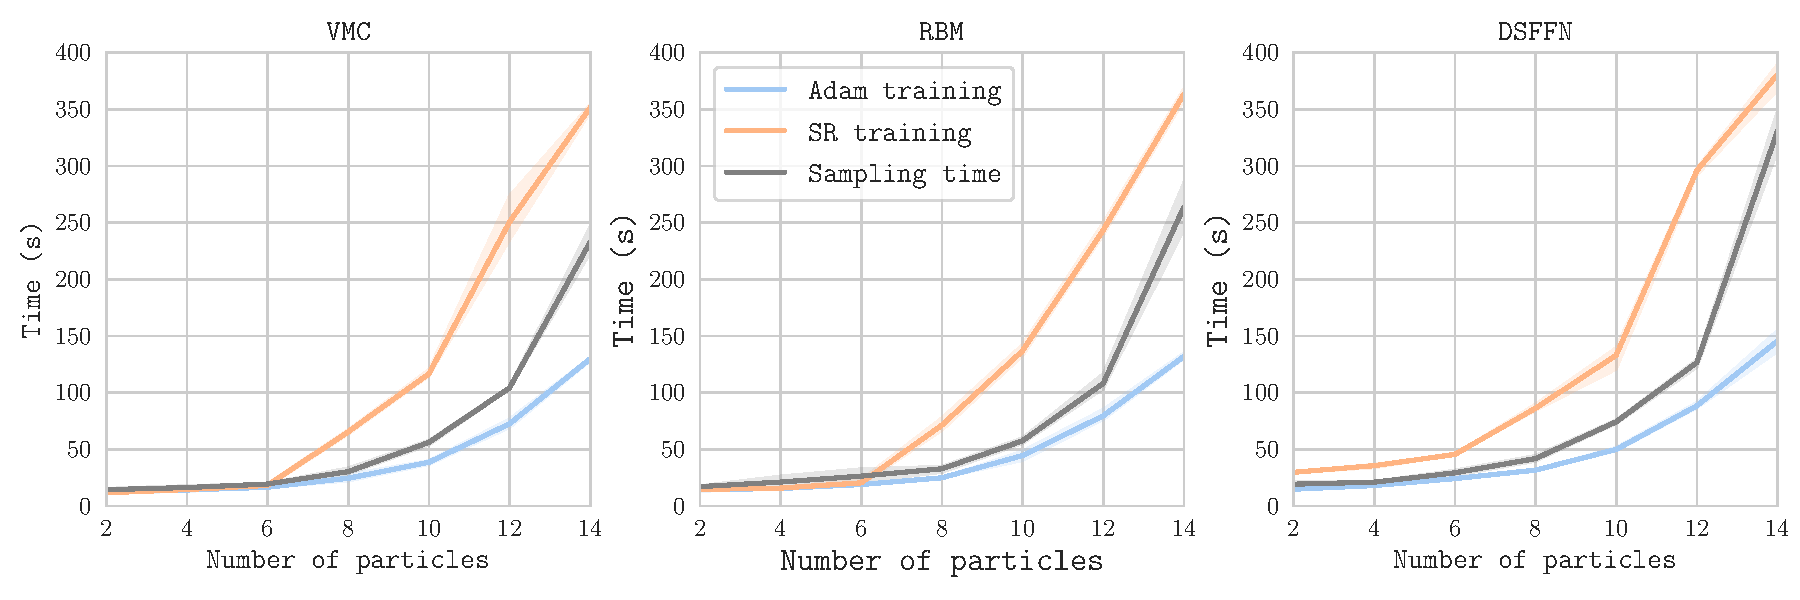
\includegraphics[width=1\linewidth]{Chapters/Results/N2/time_scaling.pdf}
    \caption{Wall time scaling in seconds as a function of number of particles, up to 14 electrons. We display separately the time for sampling and training, where the final wall time is their sum. }
    \label{fig:time_scaling}
\end{figure}

We should also mention that the sampling time does not depend on the optimiser, which is why only one common curve is displayed in \figref{fig:time_scaling}. As expected, the SR method scales worse than Adam, from the costly requirement of inverting the approximate FIM at every epoch, together with the computation of the matrix elements. 

To examine scaling estimations, we present polynomial and exponential fits of the wall time scaling in Tab \ref{tab:time_fits}. Furthermore, for each type of fit, we analyse the effects of constraining the proportionality factor to a constant value, $a = 0.5$. 
The analysis of the unconstrained coefficient reveals that the choice of optimiser, whether for the exponential or polynomial fit, does not significantly affect the order of scaling but rather impacts a constant factor. 

Theoretically, the SR in its brute-force implementation does not scale in the same order as Adam, and it is hard to say if the difference of around $0.5$ for the constrained polynomial fit is expected. While Adam's time complexity is $\mathcal{O}(N_{\theta})$ in time and space, with $N_{\theta}$ the number of parameters, SR involves a matrix inversion time complexity ($\mathcal{O}(N_{\theta}^3)$) and takes $\mathcal{O}(N_{\theta}^2)$ in space. Our block diagonal approximation of the FIM indeed reduces the time and space complexities, but there are still (smaller) matrix inversions in place, as discussed in \secref{sec:kfac}. It might be the case that some precompilation from JAX enables optimisations to take place.

If we accept the polynomial constant of $a = 0.5$, despite a worse $R^2$ score, all the methods follow a polynomial degree scaling between 2 and 3, with DSFFN being the worst and VMC the fastest as expected. A better assessment would surely require us to go beyond the 14 particles used.

Contrary to the DSFFN, the RBM and VMC do not require backpropagation under several compositions of non-linear activation functions. Also, the number of parameters are different. The VMC scales as $N\cdot d$ with particles $N$ and dimensions $d$, while the RBM scales as $N\cdot d \cdot (1 + H) + H$, where $H$ is the number of hidden nodes. For the choice of feed-forward network, the analysis is more complicated as the number of nodes changes for different layers. For timing purposes, we used architecture one from Tab. \ref{tab:arch}, which yielded good results with around $7d + L_d^2 + 8L_d +68$ parameters, where $L_d$ is the size of the latent dimension, often between four and ten.

\begin{table}[H]
    \centering
    \caption{Polynomial and exponential fits of time scaling vs. Number of Particles. The leftmost fits do not constrain any coefficients, while the leftmost fits constrains $a = 0.5$.}
    \begin{tabular}{llcccccc|cccc}
        \toprule
        \label{tab:time_fits}
        \textbf{Ansatz} & \textbf{Opt.} & \multicolumn{3}{c}{\textbf{Poly.} $(aN^b)$} & \multicolumn{3}{c}{\textbf{Exp.} $(ae^ {Nb})$} & \multicolumn{2}{c}{\textbf{Poly.} $(0.5N^b)$} & \multicolumn{2}{c}{\textbf{Exp.} $(0.5e^ {Nb})$} \\
        \cmidrule(lr){3-5} \cmidrule(lr){6-8} \cmidrule(lr){9-10} \cmidrule(lr){11-12}
        & & \textbf{a} & \textbf{b} & \textbf{R\textsuperscript{2}} & \textbf{a} & \textbf{b} & \textbf{R\textsuperscript{2}} & \textbf{b} & \textbf{R\textsuperscript{2}} & \textbf{b} & \textbf{R\textsuperscript{2}} \\
        \midrule
        \multirow{2}{*}{VMC} & Adam & 0.03 & 3.15 & 0.96 & 2.89 & 0.27 & 0.99 & 2.05 & 0.91 & 0.40 & 0.92 \\
         & SR & 0.13 & 3.01 & 0.99 & 8.09 & 0.27 & 0.98 & 2.48 & 0.97 & 0.48 & 0.84 \\
        \midrule
        \multirow{2}{*}{RBM} & Adam & 0.07 & 2.85 & 0.96 & 3.93& 0.25 & 0.99 & 2.07 & 0.93 & 0.40 & 0.88 \\
         & SR & 0.18 & 2.90 & 1.00 & 9.14 & 0.27 & 0.99 & 2.49 & 0.99 & 0.48 & 0.83 \\
        \midrule
        \multirow{2}{*}{DSFFN} & Adam & 0.17 & 2.53 & 0.93 & 5.29 & 0.24 & 0.98 & 2.10 & 0.92 & 0.41 & 0.79 \\
         & SR & 0.43 & 2.59 & 0.97 & 14.37 & 0.24 & 0.97 & 2.52 & 0.97 & 0.48 & 0.73 \\
        \bottomrule
    \end{tabular}
\end{table}

\chapter{Two-dimensional Quantum Dots}\label{ch:dots}

We now present a series of results gathered for the two-dimensional trapped fermionic system in closed-shell configuration, also known as quantum dots. A better description of the physics of this problem is given in \secref{sec:choice_of_systems}.

\section{Initial Comparisons}

\begin{figure}[H]
    \centering
    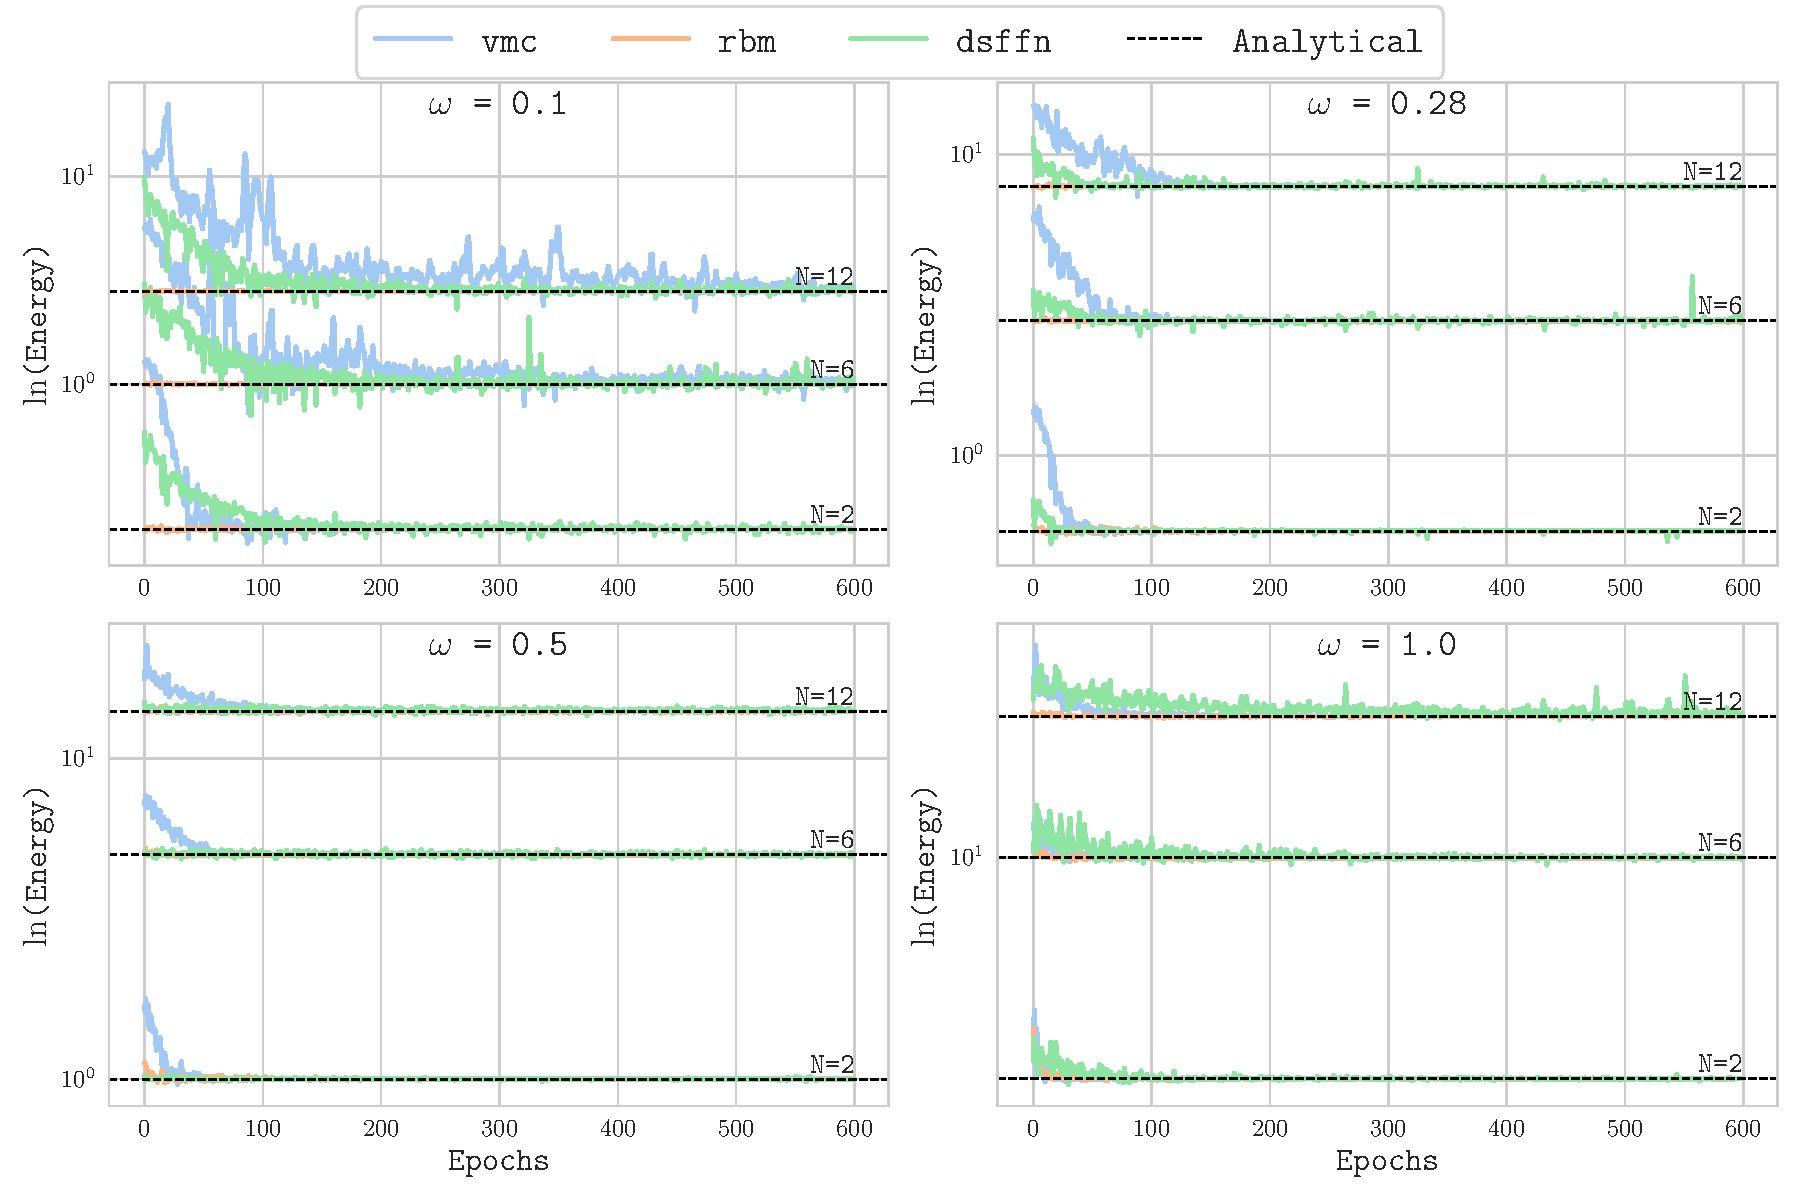
\includegraphics[width=0.9\linewidth]{Chapters/Results/dots/E_conv_ferm_dots_NI.pdf}
    \caption{Logarithmic energy convergence curve for the non-interactive problem of two-dimensional quantum dots. In black dotted line, the analytical ground state energy is marked. The three displayed models are deep set FFN (``dsffn''), restricted Boltzmann machine (``rbm'') and a standard variational Monte Carlo (``vmc''). Except for the Deep Set, Adam optimizer was used. The RBM line is hard to see as the RBM is initialised very close to the analytical solution.}
    \label{fig:E_conv_ferm_pol_NI}
\end{figure}


We again start by showing in \figref{fig:E_conv_ferm_pol_NI} that any of the models can obtain the ground state for different frequencies. We show four values of frequency, which will be used throughout the rest of the study, and we use different models and numbers of particles. Similarly to the case of the non-interacting, one-dimensional spinless fermions, we see that this task is reasonably simple, as no fine-tuning or Jastrow factors were used. We display the energy values on a logarithmic scale for the ease of comparison between energies of systems with different numbers of particles.


\section{Hyperparameter search}\label{sec:parameter_search}

In a manner similar to the one-dimensional scenario, we performed a set of hyperparameter optimisations for each of the four particle numbers tested, as detailed in \ref{met:param_search}. To avoid repetition, the individual results of these configuration sweeps are not shown, but they are comparable to what is presented in \ref{fig:ds_complete_sweep}. Unlike the one-dimensional case, we fixed the batch size at 500 proposals and the training cycles at 400 for these short experiments. The parameters tested included the presence or absence of a pre-training step, the use of the regularised gradual Coulomb interaction scheme, different correlation factors (none, Padé-Jastrow, or Jastrow), optimisers, learning rates, and different latent dimension sizes, when the DSFFN is used. It should also be noted that a frequency of $\omega = 1$ was used for all sweeps at this stage.

\subsection{Optimisers}

\begin{figure}[H]
    \centering
    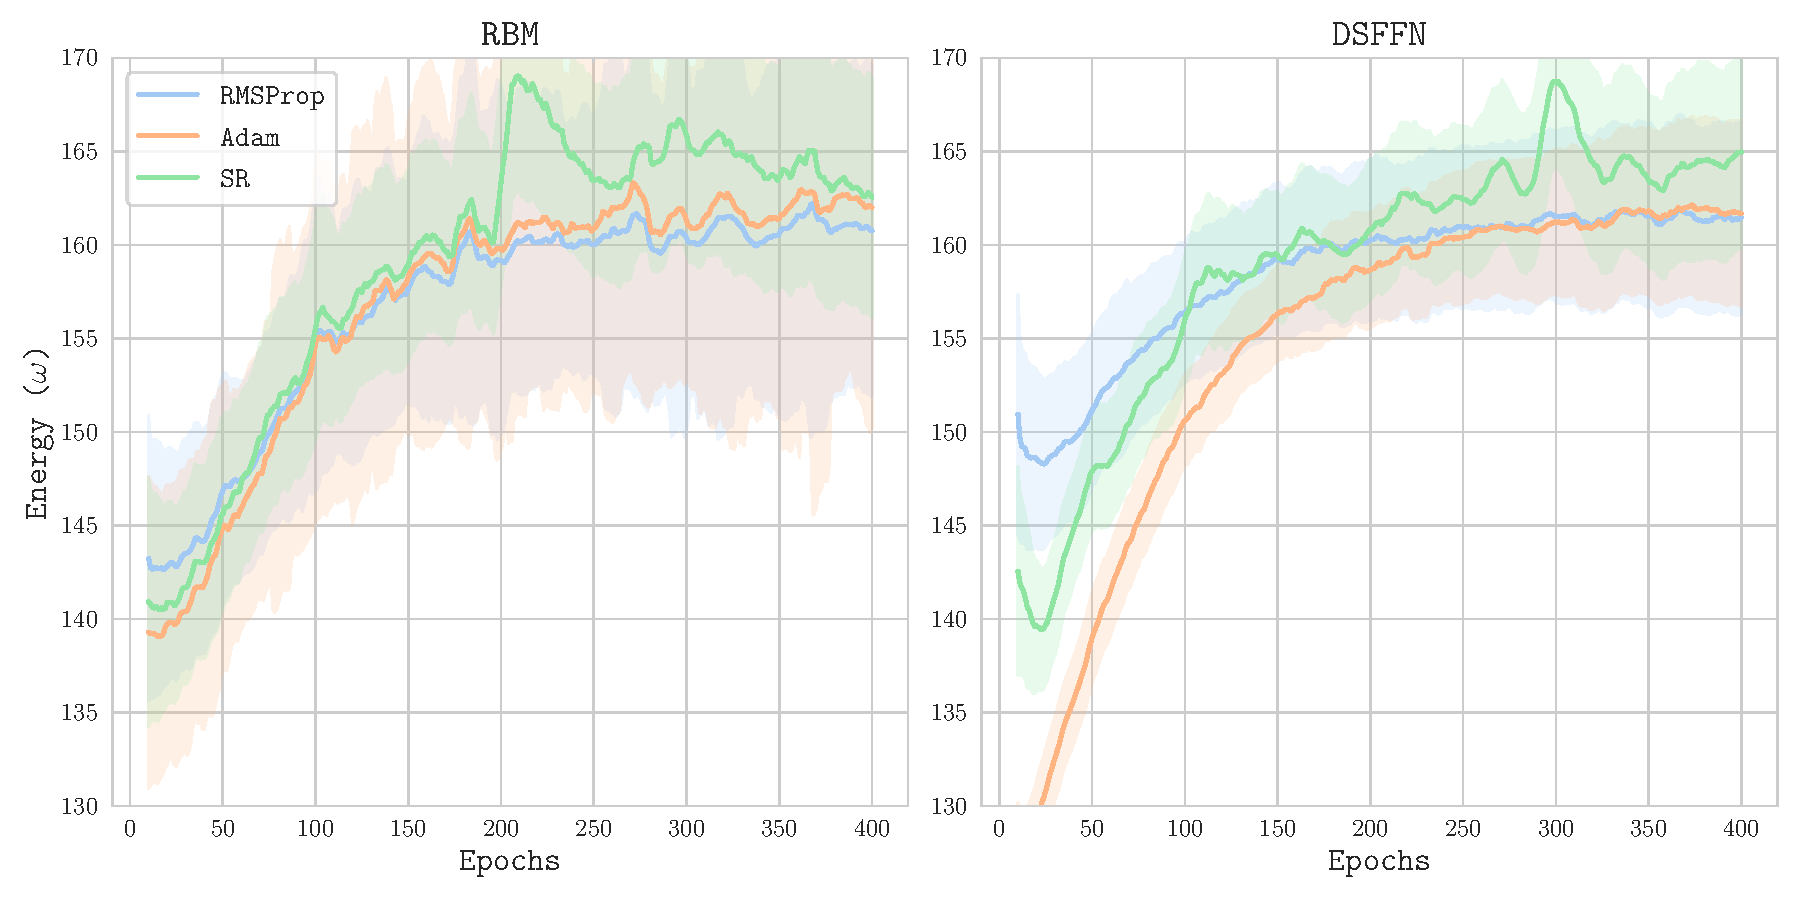
\includegraphics[width=0.9\linewidth]{Chapters/Results/dots/dsffn_vs_rbm_energy_20.pdf}
    \caption{Aggregated values over a Bayesian sweep for 20 particles and frequency of $1.0$. A similar trend is seen for both the RBM and DSFFN. The shaded region is not the error bars, but the minimum an maximum values obtained for over the sweep.}
    \label{fig:dsffn_vs_rbm_energy_20}
\end{figure}


In terms of optimiser choice, we show in \figref{fig:dsffn_vs_rbm_energy_20} the averages of 99 randomly selected parameters for a 20-particle case for the DSSFN ansatz. An analogous behaviour was observed for the two other trial functions. We note that the use of the Bayesian optimisation scheme, explained in \ref{met:param_search}, made the parameter search unbalanced and prevented the choice of stochastic reconfiguration. On that note, for the 20 particle case, SR was chosen 14 times, ADAM 25 and RMSProp was the most frequent, with 60 runs. This was seen for sweeps involving other number of particles as well, and will be further discussed. 

The reason for the infrequent SR choice is that it showed very unpredictable behaviour with respect to the choice of other parameters. When SR managed to converge, it produced good outcomes; however, its variability and often lack of convergence between different configurations were substantial. Then, despite some good individual results, on average RMSProp or Adam were favoured. For this reason, except when showing some selected results, RMSProp was the optimiser of choice for the results to follow.


\subsection{Correlation Factor}

Still investigating the averaged results over random parameters, two analysis can be made with respect to the choice of correlation factor. The following analysis for \figref{fig:corre_std} is done for a 12-particle case for the DSFFN, but the findings were the same for other choices of ansätze and number of particles. Firstly, as indicated in \figref{fig:corre_std}, the absence of any correlation factor resulted in the highest energy values, with the Jastrow factor (``j'' in the figure) producing the lowest energy and the Padé-Jastrow factor (``pj'') having the lowest energy. 

The same can be said with respect to the standard deviation of the energy, further supporting that the Padé-Jastrow factor brings us closer to the ground-state. This indicates that, without correlation factors, even using an ansatz based on parametrised neural networks does not steer us too far from the Hartree-Fock picture, where one single Slater determinant does not enable us to capture significant correlations. 

The lower energy values achieved for the Padé-Jastrow factor is also a positive theory confirmation, as it is supposed to satisfy Kato's cusp condition in a way that is not necessarily the case for the Jastrow factor \cite{huang1998spin}, while also being symmetric under particle exchange.

\begin{figure}[H]
    \centering
    \begin{subfigure}{0.84\textwidth}
        \centering
        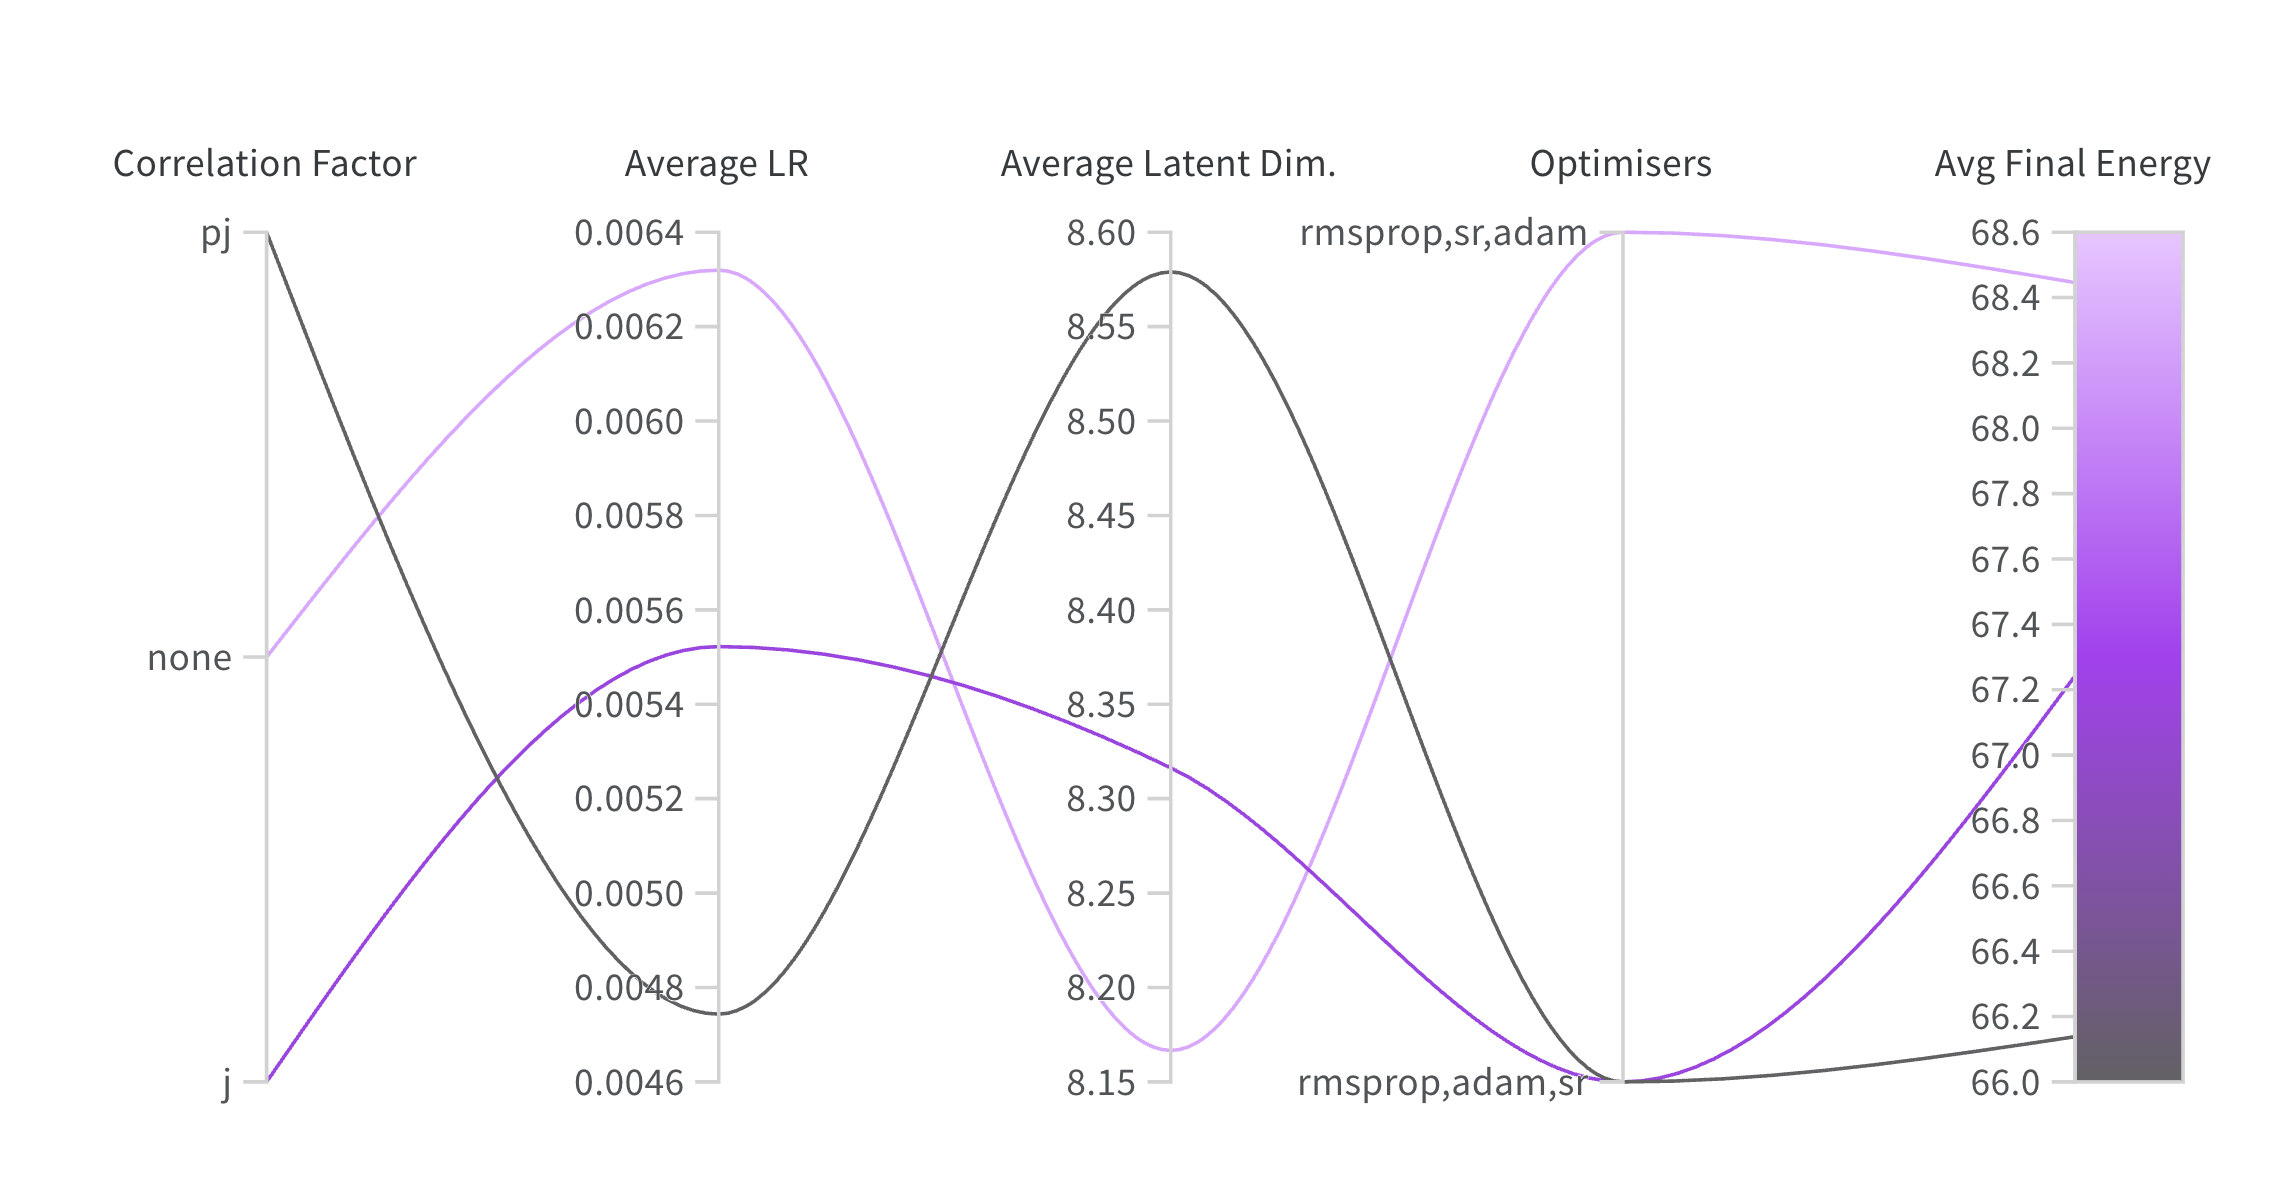
\includegraphics[width=\textwidth]{Chapters/Results/dots/n12_agg_corr.png}
    \end{subfigure}
    \begin{subfigure}{0.8\textwidth}
        \centering
        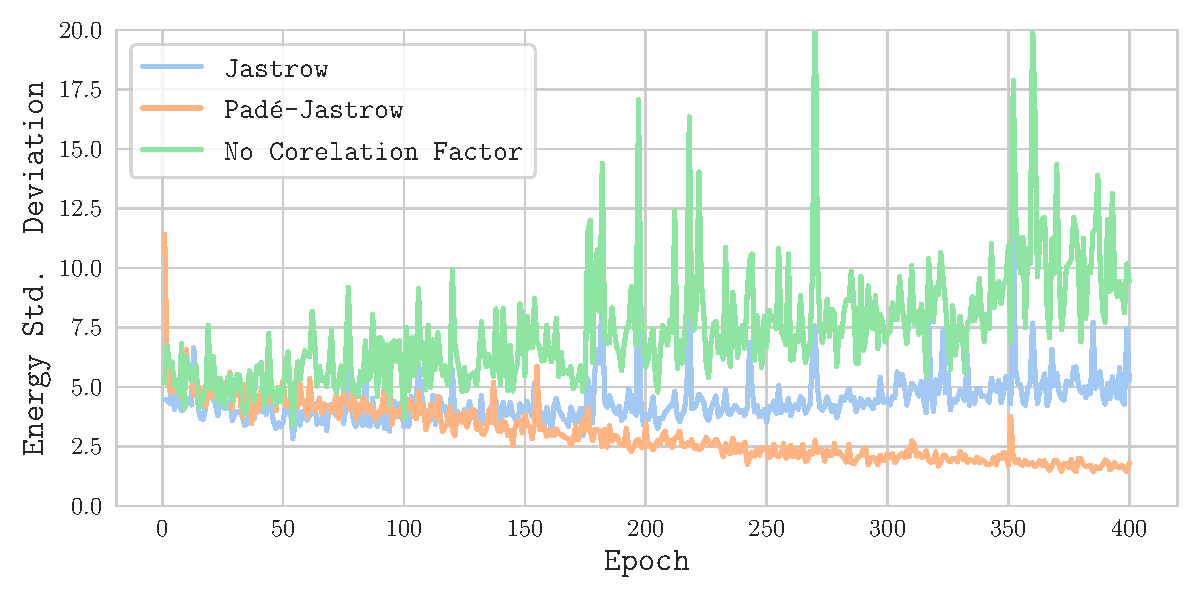
\includegraphics[width=\textwidth]{Chapters/Results/dots/correlation_factorsN_n12.pdf}
    \end{subfigure}
    \caption{Aggregated values over a Bayesian sweep and several parameters (more than what is shown in the parallel line plot) for a 12-particle system and DSFFN trial function. 165 different parameter configuration were performed.}
    \label{fig:corre_std}
\end{figure}

Lastly, an analysis can be performed with respect to the choice of correlation factor. Figure \ref{fig:coulomb_gradual} shows the effect of the correlation factor with the use of a regularised gradual Coulomb interaction potential. Despite these results only being shown for the VMC ansatz and two particles, what is evident is that consistently better results were achieved with both the use of a Padé-Jastrow factor together with the regularised gradual Coulomb interaction. This point is particularly clear when looking at the standard deviations. Although the Padé-Jastrow curve, without the regularised potential, may eventually achieve a lower minimum than the Jastrow curve after the 400 epochs displayed, this occurs much faster with the inclusion of the gradual Coulomb interaction. Again, it is evident that without a correlation factor, the results were sub-optimal in terms of both energy reduction and standard deviation.

Although we do not demonstrate it here, the combination of gradual Coulomb and the Padé-Jastrow factor was also consistently favoured when using the Deep Set network. While nonlinear activation functions theoretically allow the network to capture particle correlations, and this process is further simplified with the regularised gradual Coulomb, the results were better with the combination of these methods than with them in isolation.

\begin{figure}[H]
    \centering
    \begin{subfigure}[b]{0.8\textwidth}
        \centering
        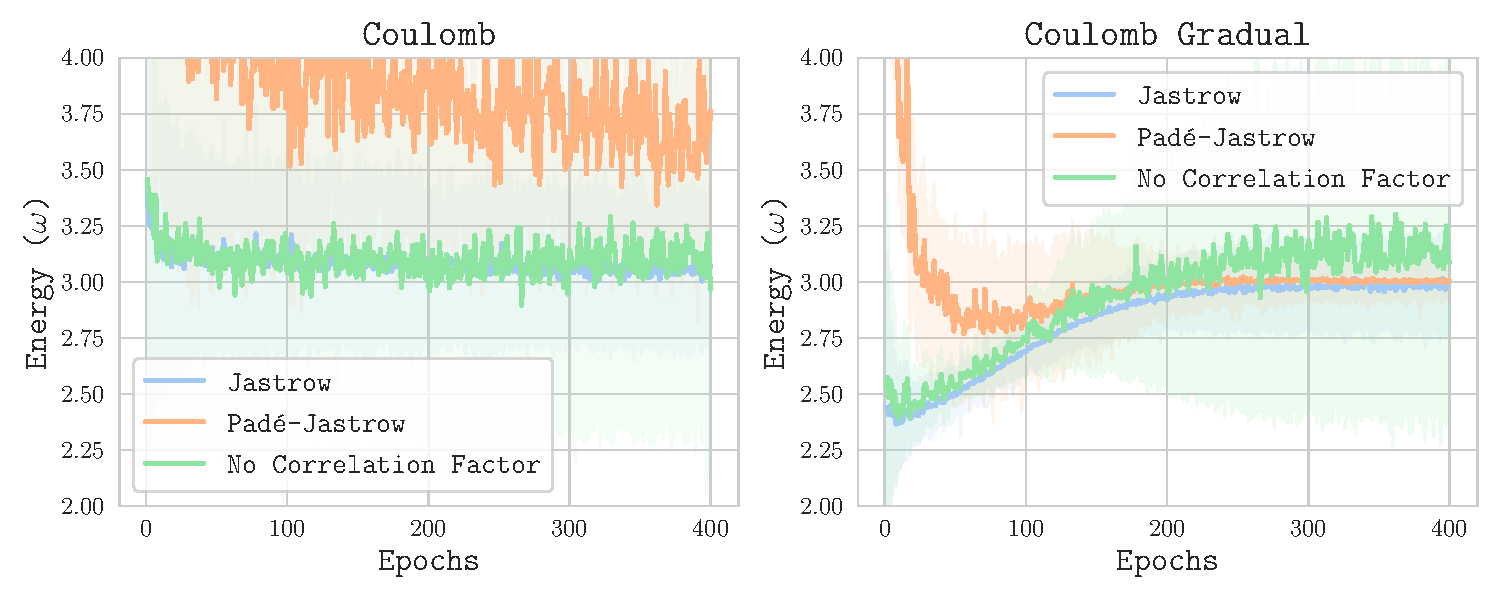
\includegraphics[width=\textwidth]{Chapters/Results/dots/n2_energy.pdf}
        \label{fig:}
        \vspace{-1cm}
    \end{subfigure}
    \begin{subfigure}[b]{0.8\textwidth}
        \centering
        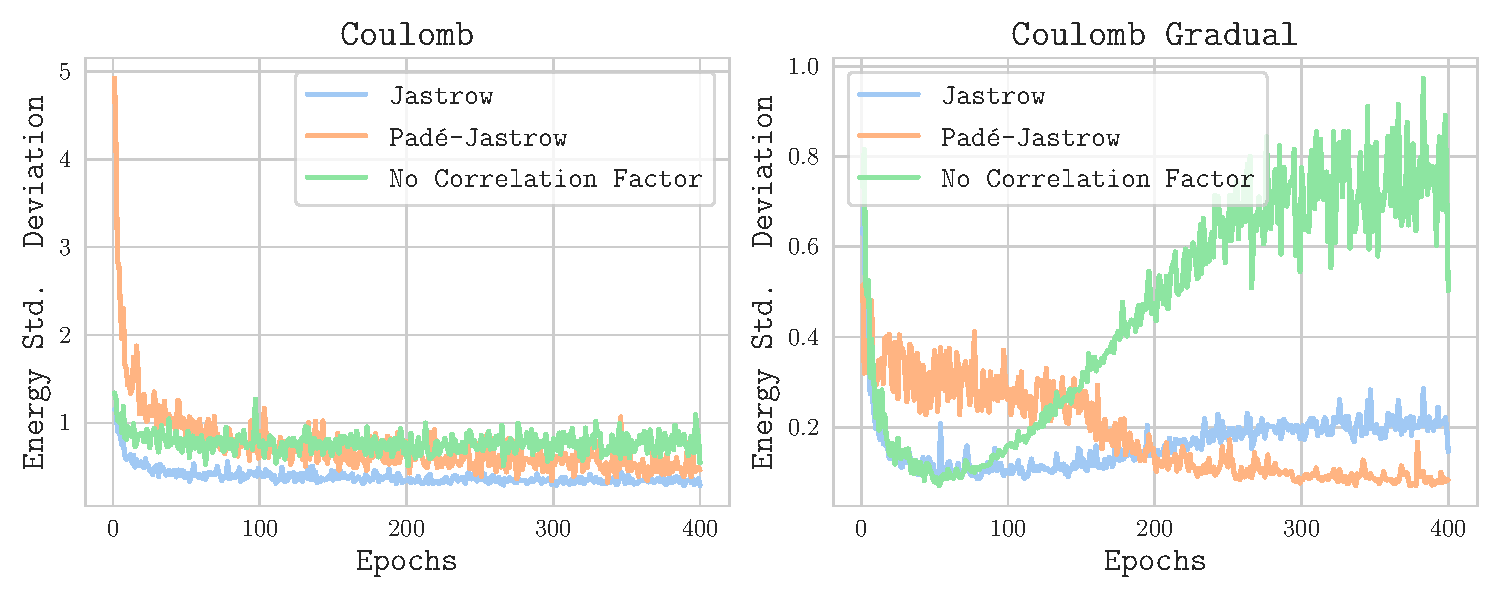
\includegraphics[width=\textwidth]{Chapters/Results/dots/n2_std.pdf}
        \label{fig:}
    \end{subfigure}
    \caption{Aggregated values over a Bayesian sweep and several parameters (see text) for the VMC ansatz and two particle case. Here, a frequency of $\omega = 1$ is selected. The shaded region is not the confidence interval, but the maximum and minimum values obtained from all parameter configurations.}
    \label{fig:coulomb_gradual}
\end{figure}

\section{One and Two-body Densities}

\begin{figure}[H]
    \centering
    \begin{subfigure}[b]{0.82\textwidth}
        \centering
        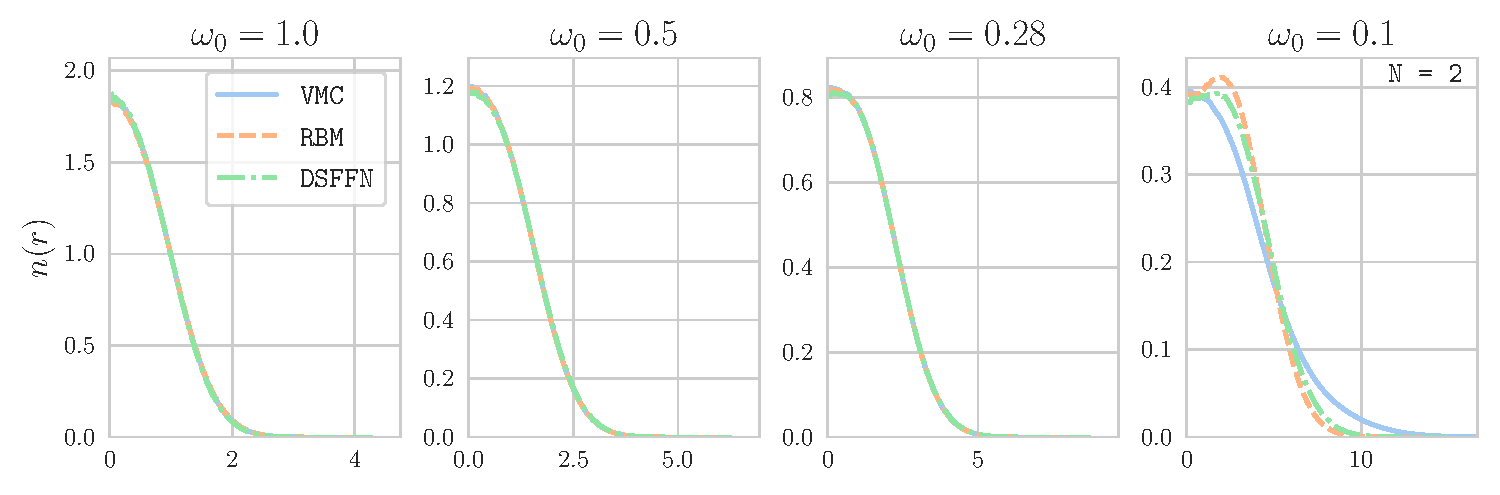
\includegraphics[width=1.0\textwidth]{Chapters/Results/dots/radial_profile_N[2]_nqs_all.pdf}
        \label{fig:total_n2}
        \vspace{-0.4cm}
    \end{subfigure}
    \begin{subfigure}[c]{0.8\textwidth}
        \centering
        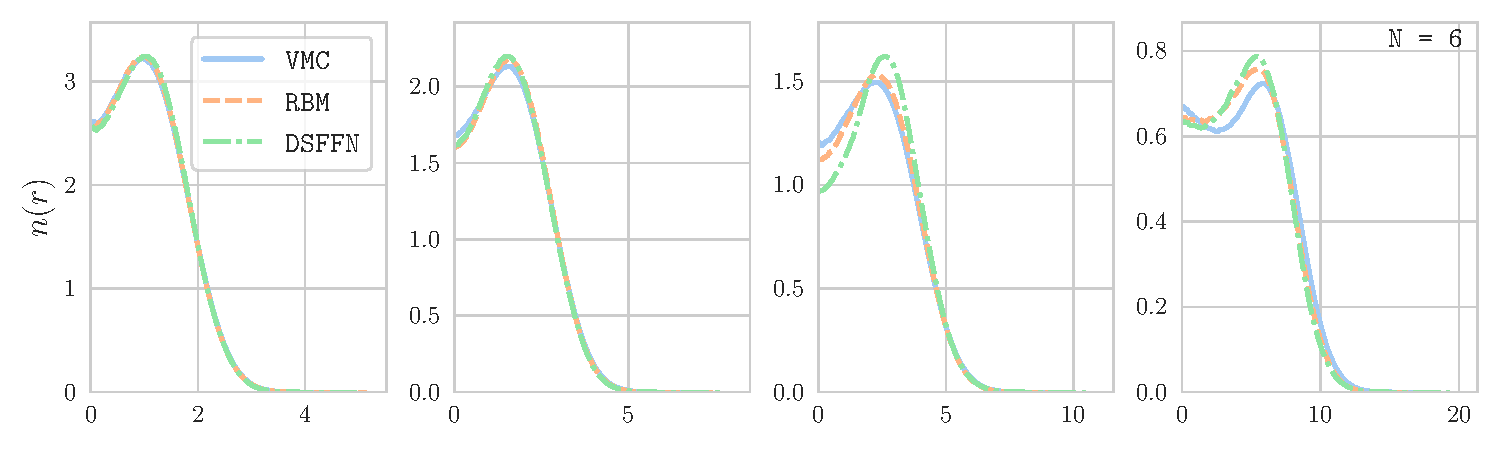
\includegraphics[width=1.0\textwidth]{Chapters/Results/dots/radial_profile_N[6]_nqs_all.pdf}
        \label{fig:total_n2}
        \vspace{-0.4cm}
    \end{subfigure}
    \begin{subfigure}[d]{0.8\textwidth}
        \centering
        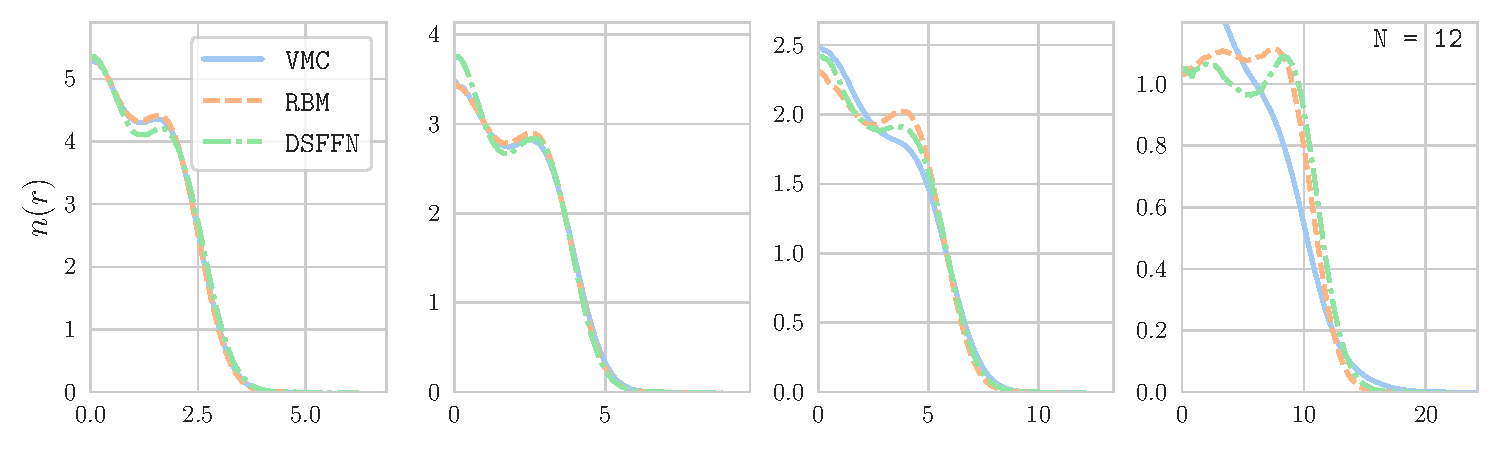
\includegraphics[width=1.0\textwidth]{Chapters/Results/dots/radial_profile_N[12]_nqs_all.pdf}
        \label{fig:total_n4}
        \vspace{-0.4cm}
    \end{subfigure}
    \begin{subfigure}[e]{0.8\textwidth}
        \centering
        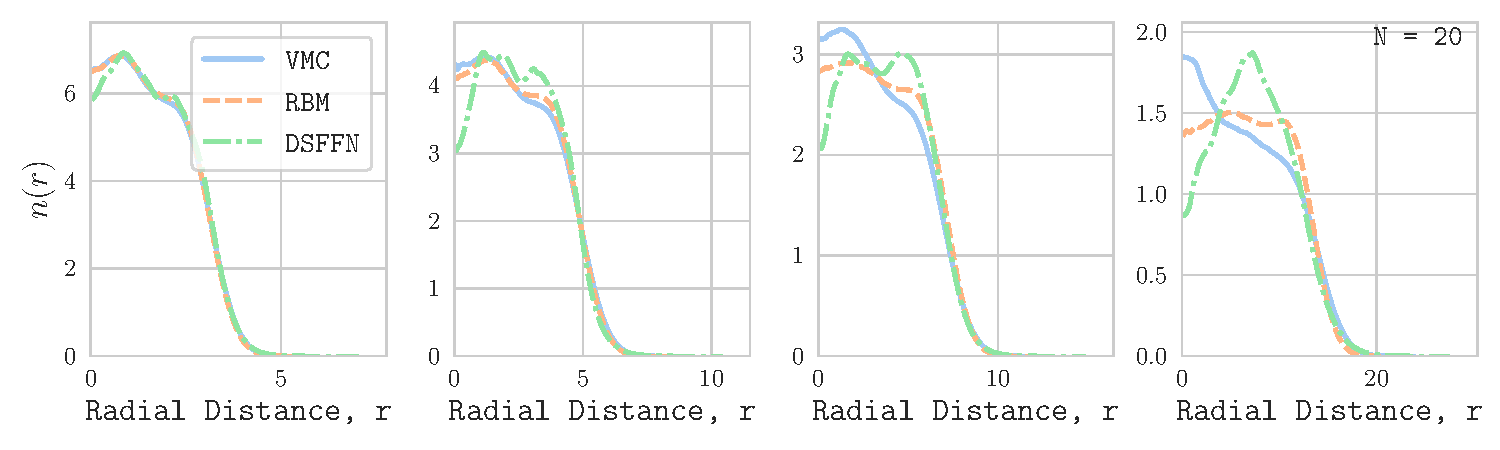
\includegraphics[width=1.0\textwidth]{Chapters/Results/dots/radial_profile_N[20]_nqs_all.pdf}
        \label{fig:total_n6}
    \end{subfigure}
    \caption{Radial density profiles for different ansätze, after $2^{24}$ MC samples. All ansätze were multiplied by a Padé-Jastrow factor, and the sampled energies can be found in Tab. \ref{tab:final_energies}}
    \label{fig:one_body_densities}
\end{figure}


In \figref{fig:one_body_densities}, we display one-body radial densities for up to 20 particles and for different frequencies. A comparison can be made in terms of the different trial functions, but all the models shown contained a Padé-Jastrow factor. It is clear that for higher frequency traps (leftmost in the plots), the radial scale significantly changes. One might overlook the fact that the plots are rescaled for consistent visibility. As expected, for higher frequencies, the particles are more localised and confined closer to the origin. In terms of particle number, again as expected, the profile heights are more pronounced with a larger number of particles, as $n(r)$ integrates to $N$. One sees that a higher density of fermions also induces more peaks in the profile. This is because there is less effective space, yet fermions still have to satisfy the exclusion principle, where fermions must occupy distinct energy levels. Then, the occupation of these levels lead to a shell structure where the fermions are forced to occupy higher energy states which leads to the fringes in the density profile.

For lower-frequency traps, we also know that the quantum energy levels become closer together. This closer spacing directly impacts the character of the fringes in the density profile. Due to the closer spacing of the energy levels, more levels must be populated because of the exclusion principle. This results in a greater number of fringes appearing in the density profile. Nevertheless, these fringes are typically less distinct and more diffuse compared to those in higher frequency traps. Despite the difficulties in capturing correlations for the low-frequency regime, all models in \figref{fig:one_body_densities} seem to replicate this in some way.

For different ansätze, there is generally good agreement for higher frequencies. This is not the case for the inferior right part \figref{fig:one_body_densities}. However, knowing which of the ansatz better represents what is expected is hard only with the density profiles, and this analysis will have to wait until we investigate the energy values.

Although unfortunate, this discrepancy between the profiles for low-frequency and higher number of particles is expected. Lower frequency traps, which are spatially wider, are particularly hard to model when the Coulomb interaction is present. This is due to the long-rage interaction of the Coulomb potential, which follows $1/r$ with $r$ the distance between the particles. Then, even when separated by large distances, the particles still significantly affect each other. This increases the complexity of the correlation, which becomes less localised. This would not be the case, for example, if instead we had a Yukawa potential, which takes the form $\exp(-kr)/r$, with $k$ being a constant. This potential decreases more rapidly as the distance between particles increases.

The exact same analysis that was performed for the radial density profile can also be done for the two-dimensional one-body densities of \figref{fig:3dobd}. We therefore do not repeat it here, but only display the 12 and 20 particle cases for a frequency of $\omega = 1.0$. The two and six particle cases can be seen in the Appendix \ref{apendix:more_results_2d}.

\begin{figure}[H]
    \centering
    % First row of subfigures
    % Second row of subfigures
    \begin{subfigure}[t]{0.32\textwidth}
        \centering
        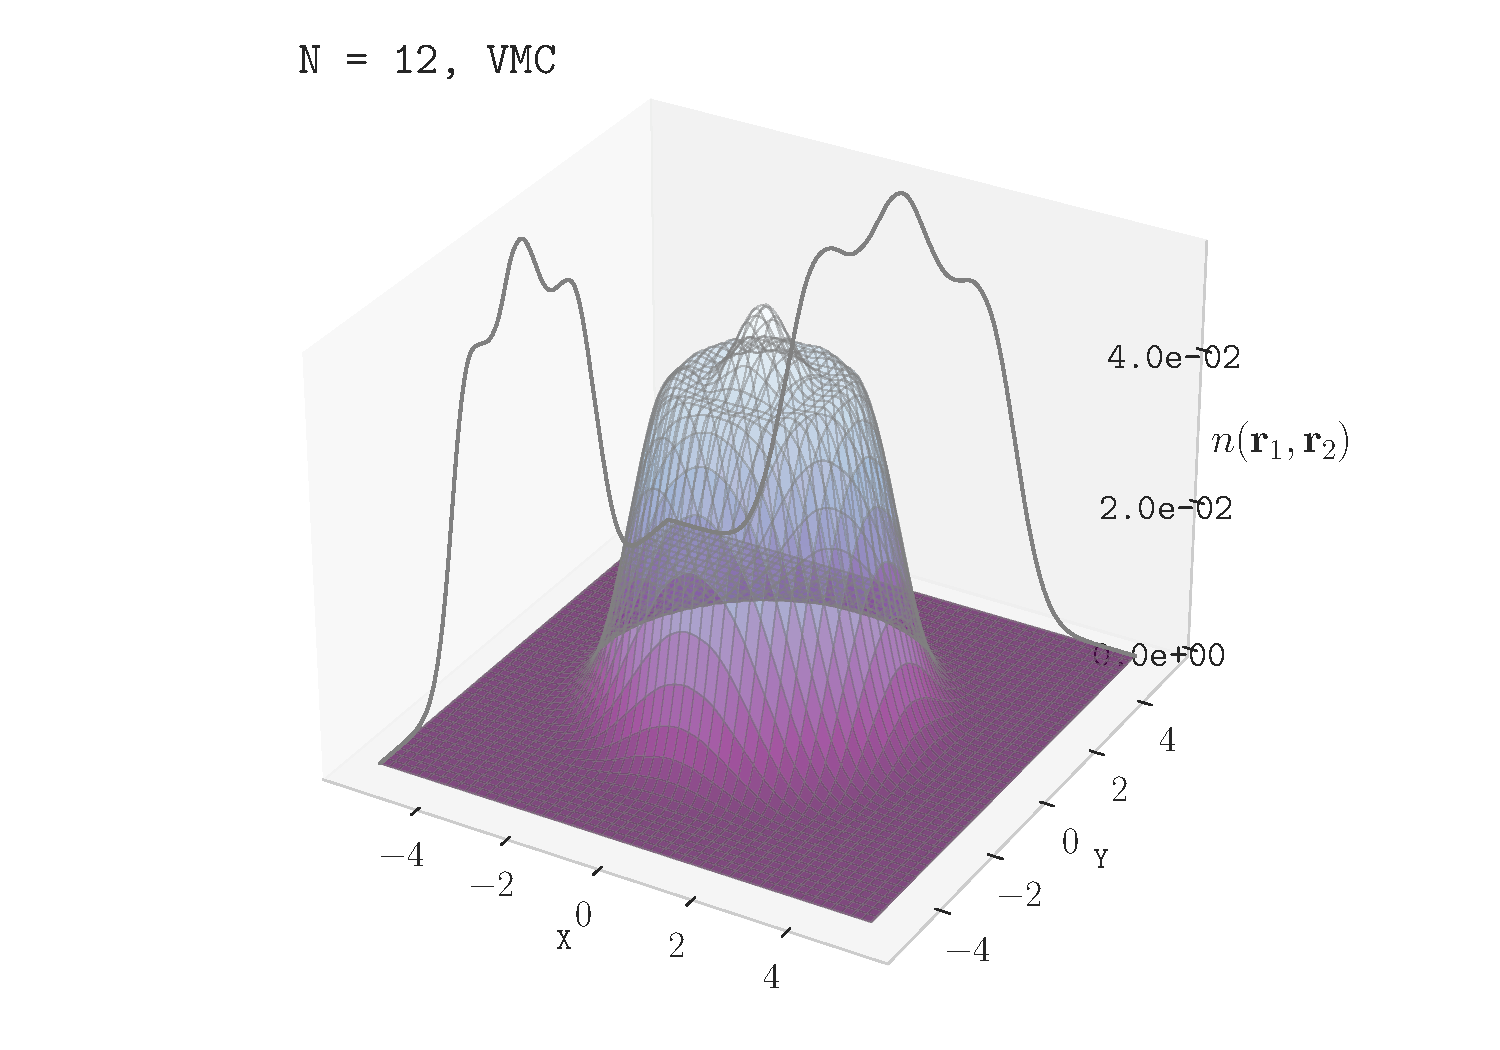
\includegraphics[width=\textwidth]{Chapters/Results/dots/density_profile_3d_N12_nqs_VMC_1.0.pdf}
        \label{fig:sub4}
    \end{subfigure}
    \begin{subfigure}[t]{0.32\textwidth}
        \centering
        \includegraphics[width=\textwidth]{Chapters/Results/dots/density_profile_3d_N12_nqs_RBM_1.0.pdf}
        \label{fig:sub5}
    \end{subfigure}
    \begin{subfigure}[t]{0.32\textwidth}
        \centering
        \includegraphics[width=\textwidth]{Chapters/Results/dots/density_profile_3d_N12_nqs_dsffn_1.0.pdf}
        \label{fig:sub6}
    \end{subfigure}
    % Third row of subfigures
    \begin{subfigure}[t]{0.32\textwidth}
        \centering
        \includegraphics[width=\textwidth]{Chapters/Results/dots/density_profile_3d_N20_nqs_VMC_1.0.pdf}
    \end{subfigure}
    \begin{subfigure}[t]{0.32\textwidth}
        \centering
        \includegraphics[width=\textwidth]{Chapters/Results/dots/density_profile_3d_N20_nqs_RBM_1.0.pdf}
    \end{subfigure}
    \begin{subfigure}[t]{0.32\textwidth}
        \centering
        \includegraphics[width=\textwidth]{Chapters/Results/dots/density_profile_3d_N20_nqs_dsffn_1.0.pdf}
    \end{subfigure}
    \caption{Two-dimensional one body density profiles for 12 and 20 particles, for all the ansätze used, all of which contained a Jastrow factor. The profiles were made from $2^{24}$ samples, and the final average energies for these can be seen in  Tab. \ref{tab:all_e_final2d}}
    \label{fig:3dobd}
\end{figure}



\begin{figure}[H]
    \centering
    % First row of subfigures
    \begin{subfigure}[t]{0.32\textwidth}
        \centering
        \includegraphics[width=\textwidth]{Chapters/Results/dots/two_body_density_N[2]_nqs_DSFFN_0.1.pdf}
        \label{fig:sub1}
    \end{subfigure}
    \begin{subfigure}[t]{0.32\textwidth}
        \centering
        \includegraphics[width=\textwidth]{Chapters/Results/dots/two_body_density_N[2]_nqs_DSFFN_0.5.pdf}
        \label{fig:sub2}
    \end{subfigure}
    \begin{subfigure}[t]{0.32\textwidth}
        \centering
        \includegraphics[width=\textwidth]{Chapters/Results/dots/two_body_density_N[2]_nqs_DSFFN_1.0.pdf}
        \label{fig:sub3}
    \end{subfigure}
    \caption{Radial two-body density profiles for the DSFFN ansatz and two particles. From left to right we have frequencies of $\omega = 0.1$, $\omega = 0.5$ and $\omega = 1.0$. The results shown were obtained from $2^{24}$ samples and 3000 training epochs with RMSProp. The densities of the first quadrant were mirrored on the three others to give a symmetric representation.}
    \label{fig:2bdensity2particle}
\end{figure}


Figure \ref{fig:2bdensity2particle} shows that the lower frequency traps, which are wider spatially, also reflect this wider profile in the two-body densities. In fact, pairs of particles are less likely to be seen in the middle of the trap with a lower frequency value. While this figure shows, for the case of two particles, how the density of two bodies changes with frequency, \figref{fig:two_body} shows how the density of two bodies depends both on the number of particles and the choice of ansatz, but now for $\omega = 0.5$.

\begin{figure}[H]
    \centering
    % First row of subfigures
    \begin{subfigure}[t]{0.32\textwidth}
        \centering
        \includegraphics[width=\textwidth]{Chapters/Results/dots/two_body_density_N[6]_nqs_VMC_0.5.pdf}
        \hspace{-1cm}
    \end{subfigure}
    \begin{subfigure}[t]{0.32\textwidth}
        \centering
        \includegraphics[width=\textwidth]{Chapters/Results/dots/two_body_density_N[6]_nqs_RBM_0.5.pdf}

        \hspace{-1cm}
    \end{subfigure}
    \begin{subfigure}[t]{0.32\textwidth}
        \centering
        \includegraphics[width=\textwidth]{Chapters/Results/dots/two_body_density_N[6]_nqs_DSFFN_0.5.pdf}
        \hspace{-1cm}
    \end{subfigure}
    % Second row of subfigures
    \begin{subfigure}[t]{0.32\textwidth}
        \centering
        \includegraphics[width=\textwidth]{Chapters/Results/dots/two_body_density_N[12]_nqs_VMC_0.5.pdf}
        \hspace{-1cm}
    \end{subfigure}
    \begin{subfigure}[t]{0.32\textwidth}
        \centering
        \includegraphics[width=\textwidth]{Chapters/Results/dots/two_body_density_N[12]_nqs_RBM_0.5.pdf}
        \hspace{-1cm}
    \end{subfigure}
    \begin{subfigure}[t]{0.32\textwidth}
        \centering
        \includegraphics[width=\textwidth]{Chapters/Results/dots/two_body_density_N[12]_nqs_DSFFN_0.5.pdf}
        \hspace{-1cm}
    \end{subfigure}
    % Third row of subfigures
    \begin{subfigure}[t]{0.32\textwidth}
        \centering
        \includegraphics[width=\textwidth]{Chapters/Results/dots/two_body_density_N[20]_nqs_VMC_0.5.pdf}
        \hspace{-1cm}
    \end{subfigure}
    \begin{subfigure}[t]{0.32\textwidth}
        \centering
        \includegraphics[width=\textwidth]{Chapters/Results/dots/two_body_density_N[20]_nqs_RBM_0.5.pdf}
        \hspace{-1cm}
    \end{subfigure}
    \begin{subfigure}[t]{0.32\textwidth}
        \centering
        \includegraphics[width=\textwidth]{Chapters/Results/dots/two_body_density_N[20]_nqs_DSFFN_0.5.pdf}
        \hspace{-1cm}
    \end{subfigure}
    \caption{Radial two-body density profiles for $\omega = 0.5$, for all ansätze and different numbers of particles. From top to bottom we have 6, 12 and 20 particles and from left to right we have VMC, RBM and DSFFN. The results shown were obtained from $2^{24}$ samples, trained with 3000 epochs with RMSProp. The densities of the first quadrant were mirrored on the three others to give a symmetric representation.}
    \label{fig:two_body}
\end{figure}

It seems that, from \figref{fig:two_body}, all models are equally capable of capturing approximately the same correlations. The density profiles exhibit a clear symmetry around the origin. Of course, this symmetry was artificially induced by us, in the process of converting the two spatial coordinates into a radial one and replicating the obtained results in the other quadrants. However, this is not an unreasonable procedure, as we see from the one-body density profiles of \figref{fig:one_body_densities} that the position distribution is radially symmetric.

We also notice that pairs of particles prefer to avoid the trap's central region due to their repulsion. As the particle count increases, there is a trend towards the localisation of particle pairs, avoiding the diagonals, which are equidistant from the origin. It appears as though the particles are avoiding the same spatial sphere, which aligns with physical intuition. This pattern is evident with 12 particles, but we observe changes as more particles are added, where they start to avoid not only diagonals but also the principal axes.

\section{Overall Energy Comparison}

\begin{figure}[H]
    \centering
    % First row of subfigures
    \begin{subfigure}{\textwidth}
        \centering
        \includegraphics[width=\textwidth]{Chapters/Results/dots/total_energy_vs_omega_n6.pdf}
        \vspace{-1.0cm}
    \end{subfigure}
    \begin{subfigure}{\textwidth}
        \centering
        \includegraphics[width=\textwidth]{Chapters/Results/dots/total_energy_vs_omega_n12.pdf}
        \vspace{-1.0cm}
    \end{subfigure}
    % Second row of subfigures
    \begin{subfigure}{\textwidth}
        \centering
        \includegraphics[width=\textwidth]{Chapters/Results/dots/total_energy_vs_omega_n20.pdf}
    \end{subfigure}
    \caption{On the left, the ratio between the measured energy and the non-interactive energy for the same system. On the right, the measure of the correlation energy, $E - E_{hf}$, where $E_{hf}$ is the Hartree-Fock energy value taken from \cite{mariadasonQuantum}. The two-particle case is too similar to the others and is shown in the Apendix \ref{apendix:more_results_2d}}
    \label{fig:correlation_energies}
\end{figure}

The right side of \figref{fig:correlation_energies} is a good reassurance that all our models used achieve energies lower than the HF energy for all ranges of frequencies. These results were gathered after training for 3000 epochs and for $2^{24}$ MC samplings. This is particularly due to the addition of the Jastrow factor in all models at this point. While all models show comparable correlation energies, the RBM model demonstrates exceptionally good performance for the 20-particle case but performs poorly for the six-particle case. The reasons for this discrepancy remain unclear, but it is likely due to sub-optimal hyperparameter choices. Typically, we would anticipate the opposite behaviour.

The fact that \figref{fig:correlation_energies} shows a correlation energy closer to 0 for lower frequency traps further supports our previous discussion about the difficulty of capturing intricate correlations due to the long-range Coulomb interaction. The larger the frequency value, the easier it is for our model to capture correlations that HF is not capable of. %due to the individual single particle Slater Determinant.

The left-hand side of \figref{fig:correlation_energies} shows that as a fraction of the non-interactive energy, all models agree well. The increase in fraction $E/E_0$ with a decrease in frequency aligns with what is found in other studies. As discussed in \cite{kroeze2016trappedelectronsquantumdegenerate}, in fact, this ratio diverges, due to its scaling as $(\omega^{-1/3})$ in the limit of $\omega \to 0$.

Finally, the proportion between energy components can be investigated in \figref{fig:fraction-energies} and in more detail for a six-particle case, in Tab. \ref{tab:fraction_energies}. Naturally, because we are in an interactive regime, the virial theorem is not expected to hold. While there is a distinct trend, a more detailed analysis would require us to investigate beyond the frequency of $1.0$ and below $0.1$. This is because, with the range investigated, we are unable to replicate the expected plateau in the ratio of $\langle K\rangle$ and $\langle V\rangle$ observed in \cite{Nordhagen2019}. The trend we observe at least indicates that with an increase in frequency comes a domination of the kinetic energy term. At low frequencies, the opposite is observed, with potential energy becoming the dominant component of the energy profile, as anticipated. This ratio decreases for larger quantum dots, where the interaction energy increases in proportion as a result of the higher particle count.

\begin{figure}
    \centering
\includegraphics[width=0.8\linewidth]{Chapters/Results/dots/energy_components_vs_omega.pdf}
    \caption{Fraction between kinetic energy and total potential energy as function of the frequency. The total potential energy corresponds to the sum of of interaction energy and the trap energy.}
    \label{fig:fraction-energies}
\end{figure}

\begin{table}[H]
    \centering
\begin{tabular}{c|c|c|c|c|c}
\toprule
\multirow{2}{*}{\textbf{Ansatz}} & \multirow{2}{*}{$\omega$} & \multirow{2}{*}{E} & \multirow{2}{*}{$\langle \hat{K}\rangle$} & \multirow{2}{*}{$\langle \hat{V}_{trap}\rangle$} & \multirow{2}{*}{$\langle \hat{V}_{int}\rangle$} \\
 & & & & & \\
\midrule
\multirow{4}{*}{dsffn} & 0.5 & 11.823(1) & 1.769(3) & 4.261(5) & 5.793(3) \\
 & 1.0 & 20.189(1) & 3.498(5) & 7.651(7) & 9.040(4) \\
 & 0.28 & 7.6481(9) & 1.008(2) & 2.756(4) & 3.884(3) \\
 & 0.1 & 3.5975(7) & 0.377(1) & 1.266(2) & 1.954(2) \\
\midrule
\multirow{4}{*}{rbm} & 0.5 & 11.8778(9) & 1.787(2) & 4.308(4) & 5.782(3) \\
 & 1.0 & 20.2826(8) & 3.539(4) & 7.658(5) & 9.086(3) \\
 & 0.28 & 7.6617(7) & 1.016(2) & 2.702(3) & 3.943(2) \\
& 0.1 & 3.5917(5) & 0.386(1) & 1.292(2) & 1.913(1) \\
\midrule
\multirow{4}{*}{vmc} & 0.5 & 11.8432(8) & 1.748(2) & 4.370(3) & 5.725(2) \\
 & 1.0 & 20.1908(8) & 3.461(4) & 7.727(5) & 9.003(3) \\
 & 0.28 & 7.6657(7) & 1.009(2) & 2.729(2) & 3.928(2) \\
& 0.1 & 3.6281(6) & 0.412(1) & 1.397(2) & 1.819(1) \\
\bottomrule
\end{tabular}
\caption{Energy components from the six particle case for the energy values displayed in \ref{tab:all_e_final2d}.}
\label{tab:fraction_energies}
\end{table}

Lastly, we display in Tab. \ref{tab:all_e_final2d} a collection of the energy values for all models at different frequencies and different numbers of particles. These values were the corresponding values associated to the body densities analysed and all plots other than the ones in the hyperparameter parameter investigation of \ref{sec:parameter_search}. It should be noted that the displayed values result from experiments conducted with a mix of common and unique parameters. Specifically, although all results were achieved after training for 3000 epochs, using RMSProp (except for the SR column), and a batch size of 1000 proposals per epoch, some experiments varied in learning rates and network architectures. This variation was unavoidable, as the scale of the system dictates the architectural choices in several instances, and for larger quantum dots, smaller learning rates were required.

\begin{table}[H]
    \centering
    \begin{tabular}{c|c|cc|c|c|c|c}
    \toprule
    N & $\omega$ & \multicolumn{2}{c|}{\textbf{DSFFN + PJ}} & \textbf{RBM + PJ} & \textbf{VMC + PJ} & \textbf{HF} \cite{mariadasonQuantum} & \textbf{DMC} \cite{hogberget2013quantum} \\
    & & SR & RMSProp & & & & \\
    \midrule
    \multirow{4}{*}{2} & 0.1 & \textbf{0.44146(4)} & 0.4463(2) & 0.44126(3) & 0.545(1) & 0.525635 & 0.44079(1) \\
    & 0.28 &\textbf{1.02218(2)} & 1.02248(4) & 1.02172(1) & 1.02257(3) & 1.14171 & 1.02164(1) \\
    & 0.5 & \textbf{1.66047(6)} & 1.66097(7) & 1.65982(1) & 1.66062129(6) & 1.79974 & 1.65977(1) \\
    & 1.0 & 3.00070(5) & 3.0023(1) & \textbf{3.00009(1)} & 3.00108(5) & 3.16190 & 3.00000(1) \\
    \midrule
    \multirow{4}{*}{6} & 0.1 & & 3.5975(7) & 3.5917(5) & 3.6281(6) & 3.85238 & 3.55385(5) \\
    & 0.28 &\textbf{7.6361(4)} & 7.6481(9) & 7.6617(7) & 7.6657(7) & 8.01957 & 7.60019(6) \\
    & 0.5 & \textbf{11.800(4)} & 11.823(1) & 11.8778(9) & 11.8432(8) & 12.271300 & 11.78484(6) \\
    & 1.0 & \textbf{20.156(7)}& 20.189(1) & 20.2826(8) & 20.1908(8) & 20.719200 & 20.15932(8) \\
    \midrule
    \multirow{4}{*}{12} & 0.1 & & \textbf{12.427(1)} & 12.445(2) & 12.678(3) & 12.9247 & 12.26984(8) \\
    & 0.28 & & 25.776(1) & \textbf{25.767(2)} & 25.937(2) & 26.5500 & 25.63577(9) \\
    & 0.5 & & 39.325(1) & \textbf{39.304(2)} & 39.318(2) & 40.2161 & 39.1596(1) \\
    & 1.0 & & 65.893(1) & 65.914(2) & \textbf{65.860(2)} & 66.9113 & 65.7001(1) \\
    \midrule
    \multirow{4}{*}{20} & 0.1 & & 30.614(4) & \textbf{30.278(3)} & 30.513(4) & 31.1902 & 29.9779(1) \\
    & 0.28 & & \textbf{62.317(2)} & 62.318(5) & 62.541(4) & 63.5390 & 61.9268(1) \\
    & 0.5 & & 94.305(2) & \textbf{94.215(4)} & 94.353(4) & 95.7328 & 93.8752(1) \\
    & 1.0 & & 156.388(3) & \textbf{156.315(4)} & 156.365(4) & 158.004 & 155.8822(1) \\
    \midrule
    \multicolumn{2}{c|}{\textbf{Average}}& & 33.5272 & 33.5058 & 33.6916 & 34.1600 & 33.3523 \\
    \bottomrule
    \end{tabular}
    \caption{Collection of the results for different frequencies and ansätze choices, in comparison to Hartree-Fock and DMC energies. The text in bold font marks the best obtained value for that row. All values were obtained with RMSProp except when shown otherwise. For training, 3000 epochs were used with batch size of 1000. For sampling, $2^{24}$ proposal steps are taken. The missing values for SR mean that we were unable to achieve convergence.}
    \label{tab:all_e_final2d}
\end{table}

All ansätze in \figref{tab:all_e_final2d} showed energy averages lower than Hartree-Fock, but higher than DMC. If we for now disregard the SR column we see that the preferred model was the RBM together with the Padé-Jastrow factor. The DSFFN network was very similar, differing by just $0.02$ on average, while the VMC had the highest energies. 

To address the use of the Stochastic Reconfiguration method, we revisit the topic briefly mentioned in the Bayesian hyperparameter search of \secref{sec:parameter_search}. When this method converged, it demonstrated great results. For instance, at a frequency of $\omega = 1.0$ with six particles, we achieved results superior to those obtained from the DMC calculations. Unfortunately, achieving such a convergence proved to be a challenge. The required parameter choices were unpredictable and lacked intuitive guidance.

One potential explanation is that the neural networks employed were simply too complex models. Although this might be a contributing factor, our experiments with smaller networks did not yield any energy convergence patterns with any of the optimisers tested. Only with more expressive and larger networks did we achieve good results beyond one-dimensional systems.

There might be an unfortunate gap in the complexities of the models tested. A 20-particle VMC ansatz used 40 variational parameters and behaved predictably based on parameter choices. For example, a smaller learning rate generally led to more stable convergence, similar to using a larger batch size. A similar argument applies to the RBM, where changing the number of hidden nodes, sometimes favoured training. An RBM we used for the 20-particle case with 6 hidden nodes displayed 200 parameters, and the Deep Set networks that we used had a similar number. However, we speculate that the non-linear activation layers significantly increased the model's complexity. While this is in general desirable, as we want to be able to capture complex pattern in data, it seems to have made the training process more difficult than expected.

%A final consideration might be made for the fact that none of the models used is guaranteed to be symmetrical or antisymmetric with respect to particle exchange. Even with the guarantee that the Deep Set implementation is sysmmetric, it must be said that the  

\section{Time Scaling Analysis}

Both \figref{fig:time_scalling2d} and Table \ref{tab:time_scalling2d} analyse the wall time scaling for the three models, only for the RMSProp optimiser. The choice of this optimiser was based on its use in presenting nearly all results for this two-dimensional system. Then, while some low-energy values were obtained with SR, we reserve its time scaling discussion for the one-dimensional system, \secref{sec:time_scaling_1d}. Here we analyse the averages over three independent runs for each measurement, with $2^{19}$ sampling steps, up to 22 particles, and for 500 training epochs.

Interestingly, \figref{fig:time_scalling2d} and Tab. \ref{tab:time_scalling2d} seem to indicate very similar polynomial-order scaling for the different trial functions. This affirmation is based on the very close values of $b$ in the polynomial or exponential fits with a constrained constant factor. In \secref{sec:time_scaling_1d} we do a more detailed analysis of how the methods scale with the number of parameters. This analysis suggests that the DSFFN should scale worse than what was measured, and we present some hypotheses as to why this is not the case. 

Firstly, there might be efficient accelerated linear algebra optimisation at play due to the use of just-in-time compilations. More importantly, the choice of architecture size for the DSFFN might have been too small. Here we measure the wall times for the smallest architecture used (architecture one in Tab. \ref{tab:arch}). This was not to be deceptive, but instead a random decision, as we needed to employ varying architectures based on the particle count and frequency to achieve optimal results.

\begin{figure}[H]
    \centering
    \includegraphics[width=1\linewidth]{Chapters/Results/dots/time_scaling_2d.pdf}
    \caption{Wall time scaling in seconds as a function of number of particles, up to 22 electrons. We display separately the time for sampling and training, where the final wall time is their sum.}
    \label{fig:time_scalling2d}
\end{figure}

For the sake of comparison, it is worth mentioning that we can evaluate our scaling against another study that implemented the same system in C++ \cite{Nordhagen2019}. In their study, they did not use automatic differentiation as we do. For their RBM, under the same constraint of $a=0.5$, they achieved a polynomial degree of approximately $b = 1.5$. This indicates that our scaling is poorer, which is expected given that we are using Python. Nevertheless, our scaling is not significantly worse, and our energy results are comparable.

\begin{table}[h!]
\centering
\caption{Polynomial and exponential fits of time scaling vs. Number of Particles. The leftmost fits do not constrain any coefficients, while the leftmost fits constrains $a = 0.5$.}
\begin{tabular}{llcccccc|cccc}
\toprule
\textbf{Ansatz} & \textbf{Opt.} & \multicolumn{3}{c}{\textbf{Poly.} $(aN^b)$} & \multicolumn{3}{c}{\textbf{Exp.} $(ae^ {Nb})$} & \multicolumn{2}{c}{\textbf{Poly.} $(0.5N^b)$} & \multicolumn{2}{c}{\textbf{Exp.} $(0.5e^ {Nb})$} \\
\cmidrule(lr){3-5} \cmidrule(lr){6-8} \cmidrule(lr){9-10} \cmidrule(lr){11-12}
& & \textbf{a} & \textbf{b} & \textbf{R\textsuperscript{2}} & \textbf{a} & \textbf{b} & \textbf{R\textsuperscript{2}} & \textbf{b} & \textbf{R\textsuperscript{2}} & \textbf{b} & \textbf{R\textsuperscript{2}} \\
\midrule
VMC & RMSProp & 0.05 & 2.76 & 0.96 & 6.60 & 0.17 & 0.98 & 2.02 & 0.94 & 0.29 & 0.93 \\
\midrule
RBM & RMSProp & 0.04 & 2.78 & 0.98 & 5.70 & 0.17 & 0.99 & 1.98 & 0.96 & 0.28 & 0.94 \\
\midrule
DSFFN & RMSProp & 0.24 & 2.32 & 0.97 & 11.68 & 0.15 & 0.99 & 2.07 & 0.96 & 0.30 & 0.89 \\
\bottomrule
\end{tabular}
\label{tab:time_scalling2d}
\end{table}
\part{Conclusion}\label{part:conclusion}

\chapter{Conclusion}

\section{Summary of Results}
The aim of this thesis project is twofold: to create a quantum computing library that is oriented towards physicists and to study the performance of the Variational Quantum Eigensolver (VQE) and the Adaptive, Problem Tailor (ADAPT) VQE to obtain some insights for the best practices in using these algorithms. 

We built Quanthon as a result, which contains the basic elements to be able to perform any quantum operation. The \texttt{Hamiltonian} class was made to allow the Hamiltonians to be entered in a low-level way by specifying the one- and two-body coefficients. Other functionalities include the \texttt{VQE} and \texttt{ADAPT-VQE} classes which are the main focus of this project, as well as different modules that can assist the quantum simulations, including the mappers to convert fermionic Hamiltonians or matrix Hamiltonians to qubit Hamiltonians, the staircase and inverted staircase algorithms for converting exponentials of Pauli strings to quantum circuits, and the expectation value estimator which simulates the measurements of the quantum circuits and computes the expectation values of the Hamiltonians. 

With the library built, we then proceeded to study the performance of the VQE with hardware efficient ansatzes and ADAPT-VQE with two different minimal complete pools, the $ V $ and the $ G $ pool defined in Subsection~\ref{sub:qubit_adapt_vqe}, through both exact energy and ideal simulations of the multiple models. With the exact energy simulation, we observed that the hardware efficient ansatz in many cases does not converge to the ground state. When it does, the relative error is usually of order $ 10^{-2} $. The ADAPT-VQE with minimal pools, however, can indeed converge to the ground state with relative error lower than $ 10^{-6} $ given enough ADAPT iterations. The number of iterations it takes for the qubit-ADAPT-VQE to converge scales roughly linearly with the number of qubits in the model and the choice of the optimiser is independent of the number of iterations required. The best optimiser for the VQE was found to be the Powell method, and the best optimiser for the qubit-ADAPT-VQE was the BFGS method. 

In the presence of shot noise, the convergence of the qubit-ADAPT-VQE slows down but is still more stable and consistently outperforms the hardware efficient ansatz. We compared the error with the expected error from the number of shots to see if the algorithms have converged. The best optimiser, in this case, is the COBYLA method for the qubit-ADAPT-VQE and the Powell method for the VQE. We noticed that the ADAPT-VQE rarely exits due to the gradient being below the tolerance level, which is likely due to the noise.

No significant differences were observed in the performances of the $ V $ and $ G $ pool, except in the case of large pairing strength the $ G $ pool converges much faster than the $ V $ pool.

Additionally, we found that the gradient for all the operators in the minimal complete pool can be $ 0 $ for many Hamiltonians if the state is initialised in the $ \ket{0} $ state. This causes the ADAPT-VQE to exit immediately without any iterations. Initialising randomly avoids this problem but causes slow convergence. First, we used the maximally superposed state as an initial state. Later, we found that by initialising the ADAPT-VQE with the optimised state from hardware efficient ansatz boosts performances by reducing the number of iterations it takes for the ADAPT-VQE to converge. 

\section{Future Work}

We will group future work into two categories: improvements to the Quanthon library and improvements to the VQE and ADAPT-VQE algorithms.

\subsection{Improvements to Quanthon}
Many functionalities can be added to the Quanthon Library, such as adding more predefined gates or other popular algorithms. We could also explore other mappers, such as the Bravyi-Kitaev transformation~\cite{Seeley2012}. To increase the speed of simulations we could parallelise the measurements and add an option to group commuting terms of the Hamiltonian to be measured simultaneously. Integration with quantum hardware could also be extremely useful to allow the library to run on real quantum devices. More ansatzes could be implemented to allow for flexibility and performance comparison, specifically the unitary coupled cluster ansatz~\cite{Romero2019} and the fermionic-ADAPT ansatz~\cite{grimsley2019}. This would allow for a more comprehensive comparison of the ansatz. Another interesting direction would be to implement noise models to allow for noisy simulations.
\subsection{Improvements to Simulation Results}
The ideal simulation takes a long time to run, therefore the maximum number of iterations was all set to below $ 30 $, the performance of the ADAPT-VQE could potentially be improved by simply allowing the algorithm to run for more iterations. The $ 0 $ gradient problem is also concerning as the initial state could cause the algorithm to exit prematurely. More research is needed to find out under which circumstance would the gradient vanish and come up with either a different operator selection criteria for choosing an operator to be appended to the ansatz, or a systematic way to select the initial state to avoid the difficulty in convergence.


\part{Appendices}
\chapter{}
\section{Left and right eigenvectors and bi-orthogonal sets.}
\label{sec:biort}
Given the eigenvalue equation, 
\begin{equation}
  A^{\mathrm{T}} y = \lambda y, 
\end{equation}
where the $n\times n$ matrix $A^{\mathrm{T}}$ is of general form. The eigenvalues $\lambda $ are 
determined by the characteristic equation,
\begin{equation}
  \mathrm{det}(A^{\mathrm{T}}-\lambda I) = \mathrm{det}(A-\lambda I) = 0,
\end{equation}
which shows that the eigenvalues of $A^{\mathrm{T}}$ are the same
as those of $A$. Consider the eigenvalue equation for the $i$'th 
eigenvector, 
\begin{equation}
  A^{\mathrm{T}} y_i = \lambda_i y_i, 
\end{equation}
then the transpose of this equation gives,
\begin{equation}
  y_i^{\mathrm{T}}A  = \lambda_i y_i^{\mathrm{T}}, 
  \label{eq:left}
\end{equation}
here $y_i^{\mathrm{T}}$ is the left eigenvector of $A$ corresponding
to the eigenvalue $\lambda_i$. The eigenvalue equation for $A$ is 
\begin{equation}
  A x_j = \lambda_j x_j, 
  \label{eq:right}
\end{equation}
where it is seen that $x_j$ is the right eigenvector of the matrix $A$ 
corresponding to the eigenvalue $\lambda_j$.
Now multiply Eq.~(\ref{eq:left}) with $x_j$ from the right and
Eq.~(\ref{eq:right}) with $y_i^{\mathrm{T}}$ from the left, and subtract to obtain,
\begin{eqnarray}
  \lambda_j y_i^{\mathrm{T}}x_j & = & \lambda_i y_i^{\mathrm{T}}x_j, \\
  \Rightarrow \: (\lambda_j -\lambda_i) y_i^{\mathrm{T}}x_j & = & 0, \\
  \Rightarrow \: y_i^{\mathrm{T}}x_j & = & 0 \:\: \mathrm{if} \lambda_i \ne \lambda_j, 
\end{eqnarray}
where it is customary to say that the 
left $y_i^{\mathrm{T}}$  and right $x_j$ eigenvectors of a 
matrix $A$ 
are \emph{bi-orthogonal} to each other.
If all $n$  
eigenvalues of the matrix $A$�are distinct, then
$y_i^{\mathrm{T}}x_j = 0 $ for $i,j = 1,2,...,n, \: i \ne j$, but 
$y_i^{\mathrm{T}}x_i \ne 0 $.  This implies that the right and left 
eigenvectors can be scaled so they form a complete set of \emph{bi-orthogonal} 
vectors.
\begin{equation}
  Y^\mathrm{T} X = \sum_{i,j=1}^n y_i^\mathrm{T}x_i = \sum_{i,j=1}^n\delta_{i,j} = 1.
\end{equation}
Here $Y^\mathrm{T}$ is a matrix whose rows are $y_i^\mathrm{T}, i=1,...,n$�and
$X$�is a matrix whose columns are $x_i, i = 1,...,n$.
This shows explicitly that $Y^\mathrm{T}$ is the inverse of $X$. 
It is clear that this works for any matrix which has a complete 
set of linearly independent eigenvectors (a nondefective matrix) 
regardless of whether the eigenvalues are distinct. 
As we have seen before, we can write in this case
\begin{displaymath}X^{-1}AX=\, {\rm diag}\, [\lambda _i]. \end{displaymath}
Indeed, if we can find any matrix $Z$ such that $Z^{-1}AZ$ is diagonal, 
then the columns of $Z$ are the right eigenvectors of $A$, and the rows of $Z^{-1}$ 
are the left eigenvectors of $A$, 
while the diagonal entries of $Z^{-1}AZ$ are the eigenvalues of $A$.
Defective matrices have an incomplete set of eigenvectors, 
and the theory requires their reduction to Jordan normal form. 

In the special case of $A$ being a complex symmetric matrix, which is
often the case in physical applications, then the left eigenvectors
are just the transpose of the right eigenvectors. In this case it is sufficient to
solve the right eigenvalue equation, and a complete set of \emph{bi-orthogonal} vectors
are obtained directly. 


\section{Three-body matrix elements in $j-j$ coupling} 
\label{sec:3matel}
Throughout this section the anti-symmetric three-, two-body 
wave functions are written as $\bar{\Psi}�$ and $\bar{\Phi}$�
respectively, while the non-anti-symmetrized functions are without 
the bar. The single-particle wave functions are given by $\phi $. 
The anti-symmetric three-body wave function may be written 
\begin{equation}
  \bar{\Psi}_{(ab)c}^{JM}(123) = {1\over \sqrt{3}}\left\{ \Psi_{(ab)c}^{JM}(123) 
  - \Psi_{(ab)c}^{JM}(132) + \Psi_{(ab)c}^{JM}(231) \right\} 
  \label{eq:threebody}
\end{equation}
here $(ab)c$ labels all relevant single particle quantum numbers  
$a = {n_a, l_a,j_a}$, and the coupling rule $\left( j_a\otimes j_b\right) _{J_{ab}}\otimes j_c$  is 
indicated.
The wave function in Eq.~\ref{eq:threebody} is 
anti-symmetric only in case where at least two of the orbits $abc$ are 
different. In the case $a=b=c$ one has to make use of  coefficients of 
fractional parentage to make the three-body wave function anti-symmetric.
 The non anti-symmetrized wave functions 
$ \Psi_{(ab)c}^{JM}(123) $ are given by 
\begin{equation}
  \Psi_{(ab)c}^{JM}(123) = \Psi\left( \bar{\Phi}_{ab}^{J_{ab}}(12)\phi_c(3); JM \right)
\end{equation}
Here $ \bar{\Phi}_{ab}^{J_{ab}}(12) $ is an anti-symmetric two-particle wave function.
\begin{equation}
  \bar{\Phi}_{ab}^{J_{ab}}(12) = {1\over \sqrt{ 2 (1+\delta_{ab})}}\sum_{m_a,m_b} 
  \langle j_a m_a, j_b m_b \vert J_{ab} M_{ab}\rangle \left( \phi_a(1) \phi_b(2) - \phi_a(2)\phi_b(1)\right)
\end{equation}
In the following derivation the total spin and projection $JM$ will 
be suppressed for notational economy. 

Consider a matrix element of the three-body wave function in Eq.~\ref{eq:threebody}
with a general interaction consisting of only two-body terms $V= V_{12} +V_{13}+V_{23}$.
\begin{eqnarray}
  \langle \bar{\Psi}_{(ab)c}(123) \vert V \vert \bar{\Psi}_{(de)f}(123)\rangle = \\
	  {1\over \sqrt{3}}\langle \Psi_{(ab)c}(123) 
	  - \Psi_{(ab)c}(132) + \Psi_{(ab)c}(231) \vert V \vert \bar{\Psi}_{(de)f}(123)\rangle
\end{eqnarray}
from the anti-symmetry follows
\begin{eqnarray}
  \langle {\Psi}_{(ab)c}(123) \vert V  \vert \bar{\Psi}_{(de)f}(123)\rangle & = &  
  \langle -{\Psi}_{(ab)c}(131) \vert V\vert \bar{\Psi}_{(de)f}(123)\rangle  \\
 & = & \langle {\Psi}_{(ab)c}(231) \vert V\vert \bar{\Psi}_{(de)f}(123)\rangle 
\end{eqnarray} 
and henceforth
\begin{eqnarray}
  \langle \bar{\Psi}_{(ab)c}(123) \vert V \vert \bar{\Psi}_{(de)f}(123)\rangle  =
  \sqrt{3}\langle {\Psi}_{(ab)c}(123) \vert V \vert \bar{\Psi}_{(de)f}(123)\rangle = \\
  \langle {\Psi}_{(ab)c}(123) \vert V_{12}\vert \Psi_{(de)f}(123)-\Psi_{(de)f}(132)+\Psi_{(de)f}(231)\rangle + \\
  2\langle {\Psi}_{(ab)c}(123)\vert V_{23}\vert \Psi_{(de)f}(123)-\Psi_{(de)f}(132)+\Psi_{(de)f}(231)\rangle 
  \label{eq:matel1}
\end{eqnarray}
Starting with the matrix element of $V_{12}$, one has
\begin{equation}
  \langle {\Psi}_{(ab)c}(123) \vert V_{12} \vert \Psi_{(de)f}(123)-\Psi_{(de)f}(132)+\Psi_{(de)f}(231)\rangle =
  V_{12}^1 + V_{12}^2 + V_{12}^3
  \label{eq:v12}
\end{equation}
where
\begin{equation}
  V_{12}^1 = \langle ab \vert V_{12} \vert  de \rangle^{AS}_{J_{ab}} \:\delta_{c,f}\:\delta_{J_{ab},J_{de}}
\end{equation}
and
\begin{equation}
  V_{12}^2+V_{12}^3 = \langle {\Psi}_{(ab)c}(123) \vert V_{12} \vert 
  -\left( \Psi_{(de)f}(132) - \Psi_{(de)f}(231) \right) \rangle
\end{equation}
recoupling $1,3 \rightarrow 1,2 $ in  $ \Psi_{(de)f}(132) $ and 
$ 2,3 \rightarrow 2,1 $ in $ \Psi_{(de)f}(231)  $ one may show by 
angular momentum algebra that 
\begin{eqnarray}
 -  \left( \Psi_{(de)f}(132) - \Psi_{(de)f}(231) \right) = \\
 \left( {1+\delta_{d,f} \over 1 + \delta_{d,e}} \right)^{1/2} \sum_{J_{df}} 
  (-1)^{j_d + J_{df}-J_{de}-J}U(j_e\:j_d\:J\:j_f; J_{de}\:J_{df})\Psi_{(df)e}(123) \\
  -\left( {1+\delta_{e,f} \over 1 + \delta_{d,e}} \right)^{1/2} \sum_{J_{ef}} 
  (-1)^{j_d + J_{ef}-J}U(j_d\:j_e\:J\:j_f; J_{de}\:J_{ef})\Psi_{(ef)d}(123) 
\end{eqnarray}
here $U(j_a\:j_b\:J\:j_c; J_{ab}\:J_{bc}) $ are the normalized Racah coefficients. 
It follows that the terms $V_{12}^2 $ and $V_{12}^3$ are given by
\begin{eqnarray}
  \nonumber
  V_{12}^2 = \left( {1+\delta_{d,f} \over 1 + \delta_{d,e}} \right)^{1/2} \sum_{J_{df}} 
  (-1)^{j_d + J_{df}-J_{de}-J}U(j_e\:j_d\:J\:j_f; J_{de}\:J_{df}) \times\\
  \langle ab\vert V_{12}\vert df\rangle_{J_{ab}}^{AS}\:\delta_{c,e}\delta_{J_{ab},J_{df}} \\
  \nonumber
  V_{12}^3 = - \left( {1+\delta_{e,f} \over 1 + \delta_{d,e}} \right)^{1/2} \sum_{J_{ef}} 
  (-1)^{j_d + J_{ef}-J}U(j_d\:j_e\:J\:j_f; J_{de}\:J_{df}) \times \\
  \nonumber
  \langle ab\vert V_{12}\vert ef\rangle_{J_{ab}}^{AS}\:\delta_{c,d}\delta_{J_{ab},J_{ef}} \\
\end{eqnarray}
Calculating the matrix element of $V_{23}$ one first recouple $1,2 \rightarrow 2,3$ in
the $\langle \mathrm{bra} \vert$.
\begin{eqnarray}
  \Psi_{(ab)c}(123) = \left( { 1\over 2(1+\delta_{a,b})} \right) \times \\
  \left\{ 
  \sum_{J_{bc}}(-1)^{j_a+J_{bc}-J}U(j_aj_bJj_c; J_{ab}J_{bc}) 
  \Psi\left( \Phi_{bc}^{J_{bc}}(23)\phi_a(1) \right) + \right. \\
    \left. \sum_{J_{ac}}(-1)^{j_a-J_{ab}+J_{ac}-J} U(j_b j_a J j_c; J_{ab} J_{ac}) 
  \Psi\left( \Phi_{ac}^{J_{ac}}(23)\phi_b(1)\right) \right\}
\end{eqnarray}
here $ \Phi_{bc}^{J_{bc}} $ and $ \Phi_{ac}^{J_{ac}} $ are non anti-symmetric two-body wave functions.
Anti-symmetric two-body matrix elements may be expressed in terms non anti-symmetric 
matrix elements by
\begin{equation}
\langle\bar{\Phi}_{ab}(12) \vert V_{12} \vert \bar{\Phi}_{cd}(12) \rangle = 
\left( {2\over (1+\delta_{ab})} \right)^{1/2}
\langle\Phi_{ab}(12) \vert V_{12} \vert \bar{\Phi}_{cd}(12) \rangle 
\end{equation}
Evaluating the matrix element of $V_{23}$ one has to evaluate the following 
matrix elements
\begin{equation}
  \langle \Psi_{(bc)a}(231) \vert V_{23} \vert \Psi_{(de)f}(123)-\Psi_{(de)f}(132)+\Psi_{(de)f}(231)\rangle
\end{equation}
and  
\begin{equation}
  \langle \Psi_{(ac)b}(231) \vert V_{23} \vert \Psi_{(de)f}(123)-\Psi_{(de)f}(132)+\Psi_{(de)f}(231)\rangle
\end{equation}
which are evaluated in the same manner as the evaluation of $V_{12}$ in Eq.~\ref{eq:v12}. 
After some angular momentum recoupling algebra in the $\vert \mathrm{ket}\rangle $, one 
ends up with the final expressions
\begin{eqnarray}
  \nonumber
  \langle \bar{\Psi}_{(ab)c}(123) \vert V \vert \bar{\Psi}_{(de)f}(123)\rangle  =
  \nonumber
  \langle ab \vert V_{12} \vert  de \rangle^{AS}_{J_{ab}} \:\delta_{c,f}\:\delta_{J_{ab},J_{de}} + \\
  \nonumber 
  \left( {1+\delta_{d,f} \over 1 + \delta_{d,e}} \right)^{1/2} 
  (-1)^{j_d - J_{de}+J_{ab}-J}U(j_ej_d J j_f; J_{de} J_{ab}) 
  \langle ab\vert v_{}\vert df\rangle_{J_{ab}}^{AS}\:\delta_{c,e} - \\
  \nonumber
  \left( {1+\delta_{e,f} \over 1 + \delta_{d,e}} \right)^{1/2} 
  (-1)^{j_d + J_{ab}-J}U(j_d j_e J j_f; J_{de} J_{ab}) 
  \langle ab\vert v_{}\vert ef\rangle_{J_{ab}}^{AS}\:\delta_{c,d} + \\
  \nonumber
  \left( { 1+\delta_{b,c} \over 1+\delta_{a,b} } \right)^{1/2}(-1)^{j_a+J_{de}-J}
  U(j_a j_b J j_c; J_{ab} J_{de})   
  \langle  bc \vert v_{} \vert de\rangle_{J_{de}}^{AS}\delta_{a,f} +  \\
  \nonumber
  \left( {1+\delta_{b,c}\over 1+\delta_{a,b} } \right)^{1/2}\sum_{J_{bc}}(-1)^{j_a+j_d-2J} 
  U(j_a j_b J j_c; J_{ab} J_{bc})   \times \\ 
  \nonumber
  \left\{ \left( {1+\delta_{d,f}\over 1+\delta_{d,e} } \right)^{1/2}(-1)^{J_{de}}
  U(j_e j_d J j_f; J_{de} J_{bc}) \langle bc \vert v_{} \vert df \rangle_{J_{bc}}^{AS}\delta_{a,e} + \right. \\ 
  \nonumber
  \left.
  \left( {1+\delta_{e,f}\over 1+\delta_{d,e}} \right)^{1/2}
  U(j_d j_e J j_f; J_{de} J_{bc}) \langle bc \vert v_{} \vert ef \rangle_{J_{bc}}^{AS}\delta_{a,d} \right\}
  + \\ 
  \nonumber
  \left( {1+\delta_{a,c}\over 1+\delta_{a,b}} \right)^{1/2}(-1)^{j_a-J_{ab}+J_{de}-J}
  U(j_b j_a J j_c; J_{ab} J_{de})   
  \langle  ac \vert v_{} \vert de\rangle_{J_{de}}^{AS}\delta_{b,f} +  \\
  \nonumber
  \left( {1+\delta_{a,c}\over 1+\delta_{a,b}} \right)^{1/2}\sum_{J_{ac}}(-1)^{j_a+j_d-J_{ab}-2J} 
  U(j_b j_a J j_c; J_{ab} J_{ac})   \times \\ 
  \nonumber
  \left\{ \left( { 1+\delta_{d,f}\over 1+\delta_{d,e}} \right)^{1/2}(-1)^{J_{de}}
  U(j_e j_d J j_f; J_{de} J_{ac}) \langle ac \vert v_{} \vert df \rangle_{J_{ac}}^{AS}\delta_{b,e} + \right. \\ 
  \left.
  \left( {1+\delta_{e,f}\over 1+\delta_{d,e}} \right)^{1/2}
  U(j_d j_e J j_f; J_{de} J_{ac}) \langle ac \vert v_{} \vert ef \rangle_{J_{ac}}^{AS}\delta_{b,d} \right\}
  \label{eq:matel2}
\end{eqnarray} 
In the case $ a = b = d = e \neq c = f $ and $ J_{ab} = J_{aa}, J_{de}={J'}_{aa}$
are even, Eq.~\ref{eq:matel2} simplifies to 
\begin{eqnarray}
  \nonumber
  \langle \bar{\Psi}_{(aa)c}(123) \vert V \vert \bar{\Psi}_{(aa)c}(123)\rangle  =
  \nonumber
  \langle aa \vert v \vert  aa \rangle^{AS}_{J_{aa}} \:\delta_{J_{aa},{J'}_{aa}} + \\
  \nonumber
  2\sum_{J_{ac}}(2J_{ac}+1) \sqrt{(2J_{aa}+1)(2{J'}_{aa} +1)} 
  \left\{ \begin{array}{ccc}
    j_a & j_a & J_{aa} \\
    j_c & J & J_{ac}�
  \end{array}\right\}
  \left\{ \begin{array}{ccc}
     j_a & j_a & {J'}_{aa} \\
    j_c & J & J_{ac}�
  \end{array}\right\}
  \langle ac \vert v \vert ac\rangle_{J_{ac}} 
\end{eqnarray}
where the normalized Racah coefficients are expressed in terms of $6-j$ symbols.
Next consider the case where all the single particle orbits in the ket are equivalent, 
i.e. $ d = e = f$,  in this case one has to make a coefficients of fractional parentage
expansion to make the three-body wave function totally anti-symmetric in the $j-j$ coupling
scheme;
\begin{equation}
  \bar{\Psi}_{ddd}(123) = \sum_K  \left. \langle j_d^2 K, j_d\vert \right\} j_d^3 J\rangle 
  \Psi_{(dd)d}(123)
\end{equation}
In this way the wave function is expressed in terms of anti-symmetric two-particle 
wave functions, and one may proceed in the same manner as for the case considered above. 
After some angular momentum recouplings, one ends up with the final 
expression for the matrix element,
\begin{eqnarray}
  \nonumber
  \langle \bar{\Psi}_{(ab)c}(123) \vert V \vert \bar{\Psi}_{(dd)d}(123)\rangle  =
  \nonumber
  \sqrt{3} \left. \langle j_d^2 J_{ab}, j_d\vert \right\} j_d^3 J\rangle  
  \langle ab \vert v \vert  dd \rangle^{AS}_{J_{ab}} \delta_{c,d} + \\
  \nonumber
  \sqrt{3}(-1)^{j_a+j_d-2J}
  \sum_K \left. \langle j_d^2 K, j_d\vert \right\} j_d^3 J\rangle \times \\
  \nonumber
  \left\{ \left( {1+\delta_{b,c}\over 1+\delta_{a,b}} \right)^{1/2} 
  \sum_{J_{bc}} U(j_a j_b J j_c; J_{ab} J_{bc})U(j_d j_dJ j_d; K J_{bc}) 
  \langle bc\vert v \vert dd\rangle_{J_{bc}}\delta_{a,d} \right. + \\
  \left. \left( {1+\delta_{a,c}\over 1+\delta_{a,b}} \right)^{1/2} 
  \sum_{J_{ac}} (-1)^{J_{ab}} U(j_b j_a J j_c; J_{ab} J_{ac})U(j_d j_dJ j_d; K J_{ac}) 
  \langle ac\vert v \vert dd\rangle_{J_{bc}}\delta_{b,d} \right\}
\end{eqnarray}



\newpage
\bibliographystyle{plain}
\bibliography{citations}
\end{document}
}
 \end{small}
\end{frame}

\begin{frame}
\begin{small}
 {\scriptsize
\beamertemplatebookbibitems
\begin{thebibliography}{10}
\bibitem{pdgvmp1993}
D.~Pfannkuche, V.~Gudmundsson, and P.~A. Maksym.
 Comparison of a hartree, a hartree-fock, and an exact treatment of
  quantum-dot helium.
 {\em Phys. Rev. B}, 47:2244--2250, 1993.
\bibitem{Raimes1972}
S.~Raimes.
 {\em Many-electron Theory}.
 North-Holland Publishing, 1972.
\bibitem{Waltersson2007}
E.~Waltersson and E.~Lindroth.
 Many-body perturbation theory calculations on circular quantum dots.
 {\em Phys. Rev. B}, 76:045314, 2007.
\bibitem{Winter2004}
J.~O. Winter.
 {\em Development and optimization of quantum dot-neuron interfaces}.
 PhD thesis, The University of Texas at Austin, 2004.
\end{thebibliography}
%\documentclass[11pt, a4paper, english]{report}

\usepackage[utf8]{inputenc}
\usepackage[T1]{fontenc}
\usepackage{babel,uiomasterfp}
\usepackage{amssymb}  % mathematical symbols (physics imports amsmath)
\usepackage{math_commands}
\usepackage{mathtools}
\usepackage{xcolor,listings,realboxes,fancyvrb} % fancyvrb for '\Verb' macro
\definecolor{mygray}{rgb}{0.8,0.8,0.8}
\definecolor{bluebell}{rgb}{0.5, 0.5, 0.74}

\lstset{
    language=Python,
    basicstyle=\ttfamily\footnotesize,
    keywordstyle=\color{codepurple}\bfseries,
    commentstyle=\color{gray}\itshape,
    stringstyle=\color{codegreen},
    frame=lines,
    numbers=left,
    numberstyle=\tiny\color{gray},
    backgroundcolor=\color{backcolour},
    tabsize=4,
    captionpos=b,
    breaklines=true,
    breakatwhitespace=false,
    showstringspaces=false,
    escapeinside={(*@}{@*)},
    columns=fullflexible,
}
\usepackage{tikz}
\usetikzlibrary{quantikz}
\usepackage{algorithmic}
\usepackage{algorithm}
%\usepackage{algpseudocode}
%\usepackage[noend]{algpseudocode}  
\usepackage[stable]{footmisc}
\usepackage{svg}
\svgpath{{Chapters/Results/}} % <- using \svgpath to avoid warning

\usepackage{graphicx}
\usepackage{subcaption}
\usepackage{multirow}
\usepackage{booktabs}

\usepackage{url}

%%%%%%%%%%%%%filtet later%%%%%%%%%%

\usepackage{listofitems} % for \readlist to create arrays
\usetikzlibrary{arrows.meta} % for arrow size
\usepackage[outline]{contour} % glow around text
\contourlength{1.4pt}

% COLORS
\usepackage{xcolor}
\colorlet{myred}{red!80!black}
\colorlet{myblue}{blue!80!black}
\colorlet{mygreen}{green!60!black}
\colorlet{myorange}{orange!70!red!60!black}
\colorlet{mydarkred}{red!30!black}
\colorlet{mydarkblue}{blue!40!black}
\colorlet{mydarkgreen}{green!30!black}
\usepackage{xcolor}

\definecolor{codegreen}{rgb}{0,0.6,0}
\definecolor{codegray}{rgb}{0.5,0.5,0.5}
\definecolor{codepurple}{rgb}{0.58,0,0.82}
\definecolor{backcolour}{rgb}{0.9,0.9,0.92}

% STYLES
\tikzset{
  >=latex, % for default LaTeX arrow head
  node/.style={thick,circle,draw=myblue,minimum size=22,inner sep=0.5,outer sep=0.6},
  node in/.style={node,green!20!black,draw=mygreen!30!black,fill=mygreen!25},
  node hidden/.style={node,blue!20!black,draw=myblue!30!black,fill=myblue!20},
  node convol/.style={node,orange!20!black,draw=myorange!30!black,fill=myorange!20},
  node out/.style={node,red!20!black,draw=myred!30!black,fill=myred!20},
  connect/.style={thick,mydarkblue}, %,line cap=round
  connect arrow/.style={-{Latex[length=4,width=3.5]},thick,mydarkblue,shorten <=0.5,shorten >=1},
  node 1/.style={node in}, % node styles, numbered for easy mapping with \nstyle
  node 2/.style={node hidden},
  node 3/.style={node out}
}
\def\nstyle{int(\lay<\Nnodlen?min(2,\lay):3)} % map layer number onto 1, 2, or 3

%%%%%%%%%%%%%%%%%%%%%%%%
\usepackage{wrapfig} %***
\usepackage{graphicx}         % include graphics such as plots


\usepackage{xcolor}
\usepackage{sectsty}
\usepackage{titlecaps}
%\usepackage{realhats}
\sectionfont{\titlecap}
\Addlcwords{and the of to as a on in}
\let\oldsubsection\subsection
\renewcommand{\subsection}[1]{\oldsubsection{\titlecap{#1}}}

\let\oldsubsubsection\subsubsection
\renewcommand{\subsubsection}[1]{\oldsubsubsection{\titlecap{#1}}}

\usepackage{indentfirst}

\definecolor{bluebell}{rgb}{0.5, 0.5, 0.74}
\chapterfont{\huge\bfseries \color{bluebell}}  % sets colour of chapters

\usepackage[paper=a4paper, left=1in, right=1in, top=1.7in, bottom=1.7in]{geometry}% http://ctan.org/pkg/geometry
\usepackage{fancyhdr}
\pagestyle{fancy}
\fancyhf{}%
\fancyhead[R]{ \nouppercase{\rightmark}}
\fancyhead[L]{ \nouppercase{\leftmark}}
\fancyfoot[R]{ \thepage}
\renewcommand{\headrulewidth}{0.1pt}

\renewcommand{\sectionmark}[1]{ \markright{#1}} 
\newcommand{\as}{antisymmetry}
\newcommand{\asc}{antisymmetric}

%gets rid of section number

\renewcommand{\vec}[1]{\mathbf{#1}}
\newcommand{\mvec}[1]{\boldsymbol{#1}}
\newcommand{\mtheta}{\mvec{\theta}}

\newcommand\blfootnote[1]{%
  \begingroup
  \renewcommand\thefootnote{}\footnote{#1}%
  \addtocounter{footnote}{-1}%
  \endgroup
}
\newcommand{\forceindent}{\leavevmode{\parindent=1em\indent}}

\renewcommand{\eqref}[1]{Eq. \ref{#1}}
\newcommand{\tabref}[1]{Tab. \ref{#1}}
\renewcommand{\figref}[1]{Fig. \ref{#1}}
\renewcommand{\secref}[1]{Sec. \ref{#1}}
\newcommand{\ssecref}[1]{Subsec. \ref{#1}}
\newcommand{\note}[1]{\textcolor{red}{(#1)}}
\newcommand{\op}[1]{\hat{\mathcal{#1}}}


% Defining a new color box
\usepackage[most]{tcolorbox}
\newtcolorbox{JTD}{colback=bluebell!10,enhanced,title=Joining the Dots,
	attach boxed title to top left={xshift=-4mm},boxrule=0pt,after skip=1cm,before skip=1cm,right skip=0cm,breakable,fonttitle=\bfseries,toprule=0pt,bottomrule=0pt,rightrule=0pt,leftrule=4pt,arc=0mm,skin=enhancedlast jigsaw,sharp corners,colframe=bluebell,colbacktitle=bluebell,boxed title style={
		frame code={ 
			\fill[bluebell](frame.south west)--(frame.north west)--(frame.north east)--([xshift=3mm]frame.east)--(frame.south east)--cycle;
			\draw[line width=1mm,bluebell]([xshift=2mm]frame.north east)--([xshift=5mm]frame.east)--([xshift=2mm]frame.south east);
			
			\draw[line width=1mm,bluebell]([xshift=5mm]frame.north east)--([xshift=8mm]frame.east)--([xshift=5mm]frame.south east);
			\fill[bluebell!40](frame.south west)--+(4mm,-2mm)--+(4mm,2mm)--cycle;
		}
	}
}


\newtcolorbox{postulate}{colback=bluebell!10,enhanced,title=Postulate,
	attach boxed title to top left={xshift=-4mm},boxrule=0pt,after skip=1cm,before skip=1cm,right skip=0cm,breakable,fonttitle=\bfseries,toprule=0pt,bottomrule=0pt,rightrule=0pt,leftrule=4pt,arc=0mm,skin=enhancedlast jigsaw,sharp corners,colframe=bluebell,colbacktitle=bluebell,boxed title style={
		frame code={ 
			\fill[bluebell](frame.south west)--(frame.north west)--(frame.north east)--([xshift=3mm]frame.east)--(frame.south east)--cycle;
			\draw[line width=1mm,bluebell]([xshift=2mm]frame.north east)--([xshift=5mm]frame.east)--([xshift=2mm]frame.south east);
			
			\draw[line width=1mm,bluebell]([xshift=5mm]frame.north east)--([xshift=8mm]frame.east)--([xshift=5mm]frame.south east);
			\fill[bluebell!40](frame.south west)--+(4mm,-2mm)--+(4mm,2mm)--cycle;
		}
	}
}



\usepackage{blindtext}
\author{Daniel Haas Becattini}
\title{\textbf{Deep Learning Methods for Quantum Many-body Systems}}
\subtitle{A study on Neural Quantum States}


\begin{document}
\uiomasterfp[program={Computational Sciences: Physics},
dept={Department of Physics}]


\newgeometry{top=1in, bottom=1in, right=0.9in, left=1.1in}
% === Preamble ===
\section*{Abstract}

The theoretical understanding behind the principles of quantum mechanics is just the first step towards solving quantum problems in real-world scenarios. Recently, a promising new field has emerged at the intersection of quantum variational methods and machine learning. This approach, named Neural Quantum States, takes advantage of neural networks as universal approximators to efficiently parametrise quantum systems.

This thesis explores the intersection of quantum many-body problems and machine learning, focussing on the application of neural network architectures to solve challenging quantum systems. We specifically investigate three methods: a standard variational Monte Carlo (VMC) parametrisation, a restricted Boltzmann machine (RBM), and a Deep Set feed-forward network (DSFFN). We applied these ansätze to two bound fermionic systems: a one-dimensional polarised fermionic system with Gaussian finite-range interaction, up to six particles and a two-dimensional quantum dots system with Coulomb interaction, up to 20 particles. The study employs Slater-Jastrow variants for the ansätze to impose fermionic antisymmetry, correlations, and cusp conditions. We experimented with various machine learning optimisation techniques, including an extensive Bayesian hyperparameter search, several well-known machine learning optimisers, and a stochastic reconfiguration, a quantum analogue of the natural gradient optimiser, known for its advantage in capturing the geometry of the quantum landscape.

Our implementation is based on Python, aiming at building a modern, modular framework with reasonable efficiency provided by using JAX as back-end. We compare the performance of these methods, discussing their strengths and limitations in representing quantum states efficiently. Our computational efficiency evaluation revealed reasonable scalability with JAX as back-end, though not matching C++ implementations as expected.

We successfully obtained ground-state energies, energy components, density profiles, and correlation energies for quantum systems replicating the results of other research studies with occasional better accuracy. Our results for 1D systems consistently surpassed Hartree-Fock and matched small-basis CI calculations. For 2D quantum dots, the addition of correlation factors repeatedly yielded lower energies than Hartree-Fock, approaching DMC calculations and even surpassing them in one instance using Stochastic Reconfiguration. We addressed the challenges of training neural networks in this unsupervised manner, highlighting the importance of reference energy values and correlation factors. Although more expressive models such as DSFFN showed excellent results, they were harder to train, requiring a balance between model complexity and user intuition. 



\newpage
\section*{Acknowledgements}

This thesis is what brought me to Oslo, but my friends are the reason I stay. I dedicate this work to all my friends and family. To those who started to love me because I came into their life and those who did not stop despite me leaving. None of this would be possible without the support of my family. None of this would be pleasant without the presence of my friends.

I would especially like to thank my supervisor, Morten Hjorth-Jensen, for all the guidance and support. Your enthusiasm and trust in whatever path I wanted to explore kept me motivated from the first day of this project onwards.

A special thank you to Nigar Abbasova, Adam Jakobsen, and Leah Hansen, for being the best second family I could have asked for. To Anna Aasen and Jonny Aarstad Igeh for taking me into the group and making me feel like I belonged somewhere, and to Hkon Kvernmoen, who, on top of that, endured my non-sensical questions about quantum mechanics, convincing me they were in fact not trivial. Finally, to everyone at CCSE: office mates, lunch companies, and table tennis rivals, thank you.

% === Table of Content ===
\tableofcontents
\newpage

% === Intro ===
\chapter{Introduction}
\section{The Quantum Many-body Problem}

Quantum mechanics stands as one of the most significant scientific achievements of the twentieth century, impacting both technological developments and our understanding of reality through its precise theoretical formalism. Despite substantial progress since the early 1920s, applying quantum mechanics to practical problems remains challenging, particularly for quantum many-body systems. These systems are central to various fields of physics, including condensed matter physics, quantum chemistry, atomic, molecular, and nuclear physics.

The core concepts of non-relativistic quantum mechanics are well condensed in the Schrödinger equation. However, the theoretical framework is only part of the challenge, and modelling even medium-sized interactive systems is a task of significant computational difficulty. This is because the dimension of a quantum system, or the Hilbert space, scales exponentially, making an exact solution of the Schrödinger equation for many-body systems unattainable. Though some classical systems also lack analytical solutions, this analysis focuses on the scaling of dimensionality, which is significantly more challenging in quantum systems.

With the advent of computers, the focus shifted towards solving the Schrödinger equation computationally and developing approximation methods to tackle larger systems. A brief description of some of the classical methods for approximating solutions follows: the Hartree-Fock (HF) method \cite{szabo2012modern}, which provides a reasonably efficient first approximation, neglects higher-order electron correlations by considering only a mean-field picture. Full Configuration Interaction (FCI) \cite{szabo2012modern} offers exact solutions within a given basis set but is computationally infeasible for large systems due to exponential scaling. Truncated Configuration Interaction (CI) methods \cite{Shavitt_Bartlett_2009} account for only some set of excitations, balancing accuracy and computational feasibility.

There are additional methods to include, but despite their effectiveness, they all face limitations in either accuracy or scalability. Configuration Interaction methods, for example, are currently restricted to around 20 particles \cite{vogiatzis2017pushing}. Both the memory required to store the Hamiltonian matrix and the computational cost of diagonalisation scale in such a manner that exceeds the capabilities of current computational resources.

In a simplistic way, solving the many-body problem means either learning to represent the high-dimensional quantum states in a more efficient way and/or learning to sample observables from them. One prominent method for specifically doing the latter is quantum Monte Carlo, which is a conceptual cornerstone of our work. Under this label, we mention variational Monte Carlo (VMC) and diffusion Monte Carlo (DMC) \cite{sorellabook}. The former optimises a parameterised guess for the wavefunction, using the variational principle to minimise the energy and obtain the ground-state. If that state is obtained, other observables can be similarly sampled. Variational Monte Carlo provides a flexible approach to incorporate complicated wavefunctions, and while it has the potential to be unbiased, its accuracy depends on the chosen ansatz. Diffusion Monte Carlo improves upon VMC, offering higher accuracy at the cost of greater computational complexity and a more heavy bias from a necessary fixed-node approximation. Therefore, it is crucial to carefully select the functional form and the number of parameters. Even if the correct representation is found, the computational cost of optimising the ansatz increases with the number of parameters. The challenge lies in how to effectively represent quantum states using parameterised functions, and machine learning offers one approach to this problem.

\section{The Many-body Problem as a Machine Learning Task}

The field of machine learning (ML), since its early days, has similarly suffered with dimensionality-exploding problems, in what is referred to as curse of dimensionality. This is because high-dimensional data are incredibly sparse, so the amount of data required for a model to make accurate predictions to unseen data grows exponentially. 

Tensor networks (TN), conceptualised in 1971, were used in quantum many-body problems in the 1990s \cite{white1992density} as perhaps the first crossover between machine learning and many-body physics. Although not developed for machine learning purposes, the connections between TN and ML are now better understood. The idea was to use area-law entanglement to build a network-like ansatz with a polynomial number of parameters. TNs further allowed for symmetries on the wavefunction to be enforced, but these methods did not generalise well beyond one-dimensional systems.

In 2017, Carleo and Troyer \cite{carleo2017solving} proposed a new type of parametrised ansatz based on a restricted Boltzmann machine, a stochastic generative neural network specifically aimed at unsupervised learning. Their approach was coined the term neural quantum states (NQS), and its success led to an investigation between tensor networks and the newly defined neural quantum states. We now know that neural quantum states display the same or higher expressive power than practical tensor networks, while being more efficient \cite{sharir2022neural}. This is because RBMs have been shown to obey volume-law scaling, which allows them to represent quantum many-body states irrespective of their level of entanglement \cite{deng2017quantum}.

RBMs are universal approximators \cite{le2008representational}, which led researchers to question if other universal approximators could equally represent quantum states with a small number of parameters. Various neural network architectures, such as convolutional neural networks, feed-forward neural networks, and graph neural networks, among others, have been shown to answer this positively \cite{lange2024architectures}. Certain NQS architectures have shown the capability to surpass classical techniques such as coupled clustering for specific systems \cite{ferminet}, while other approaches outperform state-of-the-art DMC calculations \cite{kim2023neuralnetwork}. Neural networks have also been used to accurately model excited states \cite{pfau2023natural}, and even more recently to approximate the time evolution of
quantum systems with great results \cite{lawrence2024quantum}. This evidence further points to neural networks as a promising path to solve the quantum many-body problem.

This thesis aims to explore this recent intersection between quantum many-body problems and machine learning. To do so, we compare how three methods perform in two bound fermionic systems: a one-dimensional fully polarised fermion system and a two-dimensional quantum dots system. The models tested were a standard VMC parameterisation, an RBM implementation, and a specific variant of a feed-forward network. We further explored the use of Slater-Jastrow variants for the ansätze to impose fermionic antisymmetry and correlations. The implementation was carried out using Python with JAX, inspired by their recent efficient use in quantum many-body problems \cite{vicentini2022netket, jane}.

\section{Overview and Thesis Structure}

Trying to address the presented many-body problem bears resemblance to some of the methods that we are going to address in this thesis. It is like an optimisation problem, where we try to minimise how wrong we are in our description of nature. Here, we have a space of theories or approaches, which is clearly infinite and which we test on a reference frame of arbitrary physical systems. This exploration process is non-convex, and moving in one direction brings advantages, accompanied by some disadvantages.

This thesis is not unique in its topics. Previous works have approached the same systems and have used similar methods. However, I tried to make this work personal in its didactic aspect. This means that theory is presented in a way that feels natural to me and connects points that I consider fundamental. I have tried to include here the answer to every theoretical question I asked myself along the way, with the amount of detail and rigour that at the time was sufficient to understand concepts and, eventually, move on. If a certain approach seems too big of a detour, I was probably connecting dots that for me are enlightening. If it seems too trivial, I was probably covering a gap in my knowledge. With this comes an inevitable loss in linearity of narrative, and that I tried to make evident when possible. On that note, the structure of the thesis is presented below. 

In the theory part, Chapter \ref{ch:qm_background}, provides a review of basic quantum mechanics, followed by a discussion of quantum many-body physics, and a description of the systems examined in this study. Chapter \ref{ch:computational} focusses on the computational background, from the theory of Markov chains, its connections with variational Monte Carlo, and diffusion Monte Carlo. Last in the theory section, Chapter \ref{chap:ml} starts with a theoretical treatment of statistical learning and optimisation methods. We proceed by detailing the neural networks used and finish by connecting VMC with reinforcement learning and neural quantum states.

With regard to methodology, Chapter \ref{chap:methods} provides an in-depth look at our implementations. We explain our codebase and the rationale behind certain decisions, with a minimal theoretical treatment. Further, we show how different components are integrated and how investigations were conducted.

The results are presented in Chapters \ref{ch:fermion_1d} and \ref{ch:dots}, along with discussions and a critical evaluation. Lastly, in Chapter \ref{sec:conclusion}, we assess whether the study goals were achieved and summarise the conclusions with the possibility of improvements and future research directions.









  
%\chapter*{Notation}
\label{notation}
\newlength{\notationgap}
\setlength{\notationgap}{1pc}

\typeout{START_CHAPTER "notation" \theabspage}

% Sometimes we have to include the following line to get this section
% included in the Table of Contents despite being a chapter*
\addcontentsline{toc}{chapter}{Notation}
This section provides a concise reference describing notation used throughout this
document.
If you are unfamiliar with any of the corresponding mathematical concepts,
\citet{dlbook} describe most of these ideas in
chapters 2--4.

\vspace{\notationgap}
% Need to use minipage to keep title of table on same page as table
\begin{minipage}{\textwidth}
% This is a hack to put a little title over the table
% We cannot use "\section*", etc., they appear in the table of contents.
% tocdepth does not work on this chapter.
\centerline{\bf Numbers and Arrays}
\bgroup
% The \arraystretch definition here increases the space between rows in the table,
% so that \displaystyle math has more vertical space.
\def\arraystretch{1.5}
\begin{tabular}{cp{3.25in}}
$\displaystyle a$ & A scalar (integer or real)\\
$\displaystyle \va$ & A vector\\
$\displaystyle \mA$ & A matrix\\
$\displaystyle \tA$ & A tensor\\
$\displaystyle \mI_n$ & Identity matrix with $n$ rows and $n$ columns\\
$\displaystyle \mI$ & Identity matrix with dimensionality implied by context\\
$\displaystyle \ve^{(i)}$ & Standard basis vector $[0,\dots,0,1,0,\dots,0]$ with a 1 at position $i$\\
$\displaystyle \text{diag}(\va)$ & A square, diagonal matrix with diagonal entries given by $\va$\\
$\displaystyle \ra$ & A scalar random variable\\
$\displaystyle \rva$ & A vector-valued random variable\\
$\displaystyle \rmA$ & A matrix-valued random variable\\
\end{tabular}
\egroup
\index{Scalar}
\index{Vector}
\index{Matrix}
\index{Tensor}
\end{minipage}

\vspace{\notationgap}
\begin{minipage}{\textwidth}
\centerline{\bf Sets and Graphs}
\bgroup
\def\arraystretch{1.5}
\begin{tabular}{cp{3.25in}}
$\displaystyle \sA$ & A set\\
$\displaystyle \R$ & The set of real numbers \\
% NOTE: do not use \R^+, because it is ambiguous whether:
% - It includes 0
% - It includes only real numbers, or also infinity.
% We usually do not include infinity, so we may explicitly write
% [0, \infty) to include 0
% (0, \infty) to not include 0
$\displaystyle \{0, 1, \dots, n \}$ & The set of all integers between $0$ and $n$\\
$\displaystyle [a, b]$ & The real interval including $a$ and $b$\\
$\displaystyle (a, b]$ & The real interval excluding $a$ but including $b$\\
$\displaystyle \sA \backslash \sB$ & Set subtraction, i.e., the set containing the elements of $\sA$ that are not in $\sB$\\
$\displaystyle \gG$ & A graph\\
$\displaystyle \parents_\gG(\ervx_i)$ & The parents of $\ervx_i$ in $\gG$
\end{tabular}
\egroup
\index{Scalar}
\index{Vector}
\index{Matrix}
\index{Tensor}
\index{Graph}
\index{Set}
\end{minipage}

\vspace{\notationgap}
\begin{minipage}{\textwidth}
\centerline{\bf Indexing}
\bgroup
\def\arraystretch{1.5}
\begin{tabular}{cp{3.25in}}
$\displaystyle \eva_i$ & Element $i$ of vector $\va$, with indexing starting at 1 \\
$\displaystyle \eva_{-i}$ & All elements of vector $\va$ except for element $i$ \\
$\displaystyle \emA_{i,j}$ & Element $i, j$ of matrix $\mA$ \\
$\displaystyle \mA_{i, :}$ & Row $i$ of matrix $\mA$ \\
$\displaystyle \mA_{:, i}$ & Column $i$ of matrix $\mA$ \\
$\displaystyle \etA_{i, j, k}$ & Element $(i, j, k)$ of a 3-D tensor $\tA$\\
$\displaystyle \tA_{:, :, i}$ & 2-D slice of a 3-D tensor\\
$\displaystyle \erva_i$ & Element $i$ of the random vector $\rva$ \\
\end{tabular}
\egroup
\end{minipage}

\vspace{\notationgap}
\begin{minipage}{\textwidth}
\centerline{\bf Linear Algebra Operations}
\bgroup
\def\arraystretch{1.5}
\begin{tabular}{cp{3.25in}}
$\displaystyle \mA^\top$ & Transpose of matrix $\mA$ \\
$\displaystyle \mA^+$ & Moore-Penrose pseudoinverse of $\mA$\\
$\displaystyle \mA \odot \mB $ & Element-wise (Hadamard) product of $\mA$ and $\mB$ \\
$\displaystyle \Tr{\mA}$ & Trace of $\mA$\\
% Wikipedia uses \circ for element-wise multiplication but this could be confused with function composition
$\displaystyle \mathrm{det}(\mA)$ & Determinant of $\mA$ \\
\end{tabular}
\egroup
\index{Transpose}
\index{Element-wise product|see {Hadamard product}}
\index{Hadamard product}
\index{Determinant}
\end{minipage}

\vspace{\notationgap}
\begin{minipage}{\textwidth}
\centerline{\bf Calculus}
\bgroup
\def\arraystretch{1.5}
\begin{tabular}{cp{3.25in}}
% NOTE: the [2ex] on the next line adds extra height to that row of the table.
% Without that command, the fraction on the first line is too tall and collides
% with the fraction on the second line.
$\displaystyle\frac{d y} {d x}$ & Derivative of $y$ with respect to $x$\\ [2ex]
$\displaystyle \frac{\partial y} {\partial x} $ & Partial derivative of $y$ with respect to $x$ \\
$\displaystyle \nabla_\vx y $ & Gradient of $y$ with respect to $\vx$ \\
$\displaystyle \nabla_\mX y $ & Matrix derivatives of $y$ with respect to $\mX$ \\
$\displaystyle \nabla_\tX y $ & Tensor containing derivatives of $y$ with respect to $\tX$ \\
$\displaystyle \frac{\partial f}{\partial \vx} $ & Jacobian matrix $\mJ \in \R^{m\times n}$ of $f: \R^n \rightarrow \R^m$\\
$\displaystyle \nabla_\vx^2 f(\vx)\text{ or }\mH( f)(\vx)$ & The Hessian matrix of $f$ at input point $\vx$\\
$\displaystyle \int f(\vx) d\vx $ & Definite integral over the entire domain of $\vx$ \\
$\displaystyle \int_\sS f(\vx) d\vx$ & Definite integral with respect to $\vx$ over the set $\sS$ \\
\end{tabular}
\egroup
\index{Derivative}
\index{Integral}
\index{Jacobian matrix}
\index{Hessian matrix}
\end{minipage}

\vspace{\notationgap}
\begin{minipage}{\textwidth}
\centerline{\bf Probability and Information Theory}
\bgroup
\def\arraystretch{1.5}
\begin{tabular}{cp{3.25in}}
$\displaystyle \ra \bot \rb$ & The random variables $\ra$ and $\rb$ are independent\\
$\displaystyle \ra \bot \rb \mid \rc $ & They are conditionally independent given $\rc$\\
$\displaystyle P(\ra)$ & A probability distribution over a discrete variable\\
$\displaystyle p(\ra)$ & A probability distribution over a continuous variable, or over
a variable whose type has not been specified\\
$\displaystyle \ra \sim P$ & Random variable $\ra$ has distribution $P$\\% so thing on left of \sim should always be a random variable, with name beginning with \r
$\displaystyle  \E_{\rx\sim P} [ f(x) ]\text{ or } \E f(x)$ & Expectation of $f(x)$ with respect to $P(\rx)$ \\
$\displaystyle \Var(f(x)) $ &  Variance of $f(x)$ under $P(\rx)$ \\
$\displaystyle \Cov(f(x),g(x)) $ & Covariance of $f(x)$ and $g(x)$ under $P(\rx)$\\
$\displaystyle \KL ( P \Vert Q ) $ & Kullback-Leibler divergence of P and Q \\
$\displaystyle \mathcal{N} ( \vx ; \vmu , \mSigma)$ & Gaussian distribution %
over $\vx$ with mean $\vmu$ and covariance $\mSigma$ \\
\end{tabular}
\egroup
\index{Independence}
\index{Conditional independence}
\index{Variance}
\index{Covariance}
\index{Kullback-Leibler divergence}
\index{Shannon entropy}
\end{minipage}

\vspace{\notationgap}
\begin{minipage}{\textwidth}
\centerline{\bf Functions}
\bgroup
\def\arraystretch{1.5}
\begin{tabular}{cp{3.25in}}
$\displaystyle f: \sA \rightarrow \sB$ & The function $f$ with domain $\sA$ and range $\sB$\\
$\displaystyle f \circ g $ & Composition of the functions $f$ and $g$ \\
  $\displaystyle f(\vx ; \vtheta) $ & A function of $\vx$ parametrized by $\vtheta$.
  (Sometimes we write $f(\vx)$ and omit the argument $\vtheta$ to lighten notation) \\
$\displaystyle \log x$ & Natural logarithm of $x$ \\
$\displaystyle \sigma(x)$ & Logistic sigmoid, $\displaystyle \frac{1} {1 + \exp(-x)}$ \\
$\displaystyle \zeta(x)$ & Softplus, $\log(1 + \exp(x))$ \\
$\displaystyle || \vx ||_p $ & $\normlp$ norm of $\vx$ \\
$\displaystyle || \vx || $ & $\normltwo$ norm of $\vx$ \\
$\displaystyle \1_\mathrm{condition}$ & is 1 if the condition is true, 0 otherwise\\
\end{tabular}
\egroup
\index{Sigmoid}
\index{Softplus}
\index{Norm}
\end{minipage}

Sometimes we use a function $f$ whose argument is a scalar but apply
it to a vector, matrix, or tensor: $f(\vx)$, $f(\mX)$, or $f(\tX)$.
This denotes the application of $f$ to the
array element-wise. For example, if $\tC = \sigma(\tX)$, then $\etC_{i,j,k} = \sigma(\etX_{i,j,k})$
for all valid values of $i$, $j$ and $k$.


\vspace{\notationgap}
\begin{minipage}{\textwidth}
\centerline{\bf Datasets and Distributions}
\bgroup
\def\arraystretch{1.5}
\begin{tabular}{cp{3.25in}}
$\displaystyle \pdata$ & The data generating distribution\\
$\displaystyle \ptrain$ & The empirical distribution defined by the training set\\
$\displaystyle \vx^{(i)}$ & The $i$-th example (input) from a dataset\\
$\displaystyle y^{(i)}\text{ or }\vy^{(i)}$ & The target associated with $\vx^{(i)}$ for supervised learning\\
$\displaystyle \mX$ & The $m \times n$ matrix with input example $\vx^{(i)}$ in row $\mX_{i,:}$\\
\end{tabular}
\egroup
\end{minipage}

\clearpage

\typeout{END_CHAPTER "notation" \theabspage}  

% === Theory ===
\part{Theory}\label{part:theory}
\chapter{Quantum Physics Background}\label{ch:qm_background}

\begin{figure}[h]
    \centering
    \includegraphics[width=0.8\linewidth]{Chapters/Theoretical_Background/images/QM_section_cover.pdf}
    \caption{Wigner quasi-probability function $W$ as function of position $q$ and momentum $p$.}
    \label{fig:QM_section_cover}
\end{figure}

%=============================================================
\section{Basic Linear Algebra background}
\subsubsection{Dirac Notation and Completeness}
We start with a basic review of linear algebra for two main reasons. First, we want to emphasise that from the beginning we are dealing with complex n-dimensional vector spaces, sub-spaces of $\mathbb{C}^n$, so that an element $\mvec{z} \in \mathbb{C}^N$ can be represented as an n-tuple $(z_1, z_2, ..., z_n)$ where $z_i$ is a complex number. Second, we want to migrate to the standard Dirac notation as soon as possible, showing what it means and why we are doing it.

Using the Dirac notation, we represent a standard basis for the vector space $\{e_i\}$ with ket vectors, written as $\{\ket{i}\}$, with $i \in \mathbb{N}$. A generic vector $\ket{a}$ in this space can be decomposed in terms of a complete basis as
\begin{align*}
    \ket{a} =  \sum_i \ket{i}a_i = \sum_i \ket{i}\bra{i}\ket{a}.
\end{align*}

In the second equality, the completeness of the basis is apparent, which can be represented as 
\begin{align*}
    I =  \sum_i\ket{i}\bra{i},
\end{align*}
with $I$ being the identity matrix. This completeness relation is crucial in quantum mechanics because it guarantees that the basis spans the entire vector space, allowing the decomposition of a general $\ket{a}$.

\subsubsection{Operators and Adjoint Operators}
A linear operator $\op{O}$ is a mathematical object that maps one vector to another. We say it ``acts'' on a vector $\ket{a}$, returning another vector, as in $ \op{O}\ket{a}=\ket{b}$. We can also define the adjoint of this operator as the operator that maps the dual \cite{curtis2012linear} of vector $\ket{a}$ to the dual of vector $\ket{b}$. In Dirac notation, this can be written $ \bra{a} \op{O}^\dagger =\bra{b}$. Furthermore, in quantum-mechanical contexts, the dual of the ket vector is called a bra vector, and we denote it $\bra{a} = \ket{a}^\dagger$. This way, an inner product is written $\bra{a}\ket{b} \coloneqq \braket{a}{b}$.

For an operator to be called linear, it must obey the following linearity property:
\begin{align*}
    \op{O}(x\ket{a} + y\ket{b}) = x\op{O}\ket{a} + y\op{O}\ket{b},
\end{align*}
where $x,\,y$ are scalars. One fundamental aspect of linear operators is that, given a choice of a basis $\{\ket{i}\}$, we can represent them as matrices. Thus, the linear transformation can be viewed as a matrix-vector multiplication: 
\begin{align*}
    \op{O}\ket{i} = \sum_{j} \ket{j}O_{ji}.
\end{align*}

To obtain the matrix elements of the matrix representation of the operator $\op{O}$ we can consider the inner product of different basis vectors:
\begin{align*}
   O_{ki} = \bra{k}\op{O}\ket{i} = \sum_{j} \braket{k}{j}O_{ji},
\end{align*}
where $\ket{k}$ and $\ket{j}$ are basis vectors in the vector space on which $\op{O}$ acts. The subsequent application of linear operators can similarly be expressed as subsequent matrix multiplications, which means that if $\op{C} = \op{A}\op{B}$, then
\begin{align*}
C_{ij} = \sum_k A_{ik}B_{kj}.
\end{align*}

From that it is clear that $\op{A}\op{B} \neq \op{B}\op{A}$ in general. This distinction can seem obvious, but deserves special attention for its implications in quantum mechanics. Let us define the commutator of operators:
\begin{align*}
    [\op{A},\, \op{B}] = \op{A} \op{B} - \op{B}\op{A}.
\end{align*}

When the commutator of two operators is zero, they are said to commute with each other.

\begin{JTD}
\footnote{Since we are assuming some prior knowledge, we introduce these boxes, in which we connect what is presented with not yet defined concepts. This is a clear compromise in linearity of narrative to make the reading more interesting for those with prior knowledge.}When two operators commute,
    \begin{itemize}
        \item the sequence of measurements does not affect the result;
        \item it is possible to find states that are eigenstates for both operators, meaning we can know the outcome for both measurements precisely and simultaneously;
        \item if an operator commutes with a special operator we call the Hamiltonian ($\hat{H}$), it can be associated with a conserved physical quantity.
    \end{itemize}
\end{JTD}

\subsubsection{Additional Matrix Properties}
Linear algebra is the language of quantum mechanics. As such, there are several properties of matrices that need to be mentioned, even if they seem to appear with no motivation for now.
\begin{itemize}
    \item \textbf{Hermitian Matrices:} If a matrix $A$ is such that $A^\dagger = A$, it is called Hermitian. In quantum mechanics, this is relevant because every observable can be represented by a Hermitian operator. 
    \item \textbf{Unitary Matrices:} If a matrix $A$ is such that its inverse is equal to its adjoint ($A^{-1} = A^{\dagger}$) it is called a unitary matrix. This is relevant because unitary operators preserve the inner product ($\langle Ax, Ay\rangle =\langle x, y\rangle $) and vector norms. Consequently, they preserve probability amplitudes.
    \item \textbf{Orthogonal Matrices:} A unitary matrix with real elements is called orthogonal. They are important because they represent transformations that do not break the orthogonality of vectors - a crucial point in coordinate transformations.
\end{itemize}

\subsection{Hilbert spaces}
Quantum and classical mechanical states are different conceptual objects. Unlike a classical state, a general quantum state \textbf{needs} to be represented as elements of a vector space known as a Hilbert space. In Newtonian mechanics, the vector spaces used are Euclidean. In contrast, Hilbert vector spaces have some major differences.

First, Euclidean vector spaces are vector spaces over the real numbers, while Hilbert spaces are more generally defined over the complex field.
Additionally, Euclidian spaces are finite-dimensional, whereas Hilbert spaces generalise the idea of an inner product to infinite dimension.
Finally, Hilbert spaces require us to be more precise with the concept of sequence convergence. In particular, a Hilbert space must be Cauchy-complete. Intuitively, this means that every sequence that ``seems like'' it should converge (to another element of the space) in fact does. 

This third difference is more subtle because we get it for free in Euclidian spaces \cite{rudin}, and thus, it does not often cross our minds - Euclidian spaces inherit Cauchy completeness from the real numbers.

We do not intend to be rigorous in our definition of a Hilbert space, and a complete discussion is found in \cite{rudin}. We care about the convergence of sequences because we want to use calculus in this vector space, and, therefore, limits have to be well defined. Furthermore, we often want to expand quantum states as an infinite sum of eigenvectors of an observable, again requiring a precise definition of limits.

\subsection{From Euclidian vectors to functions}
In this section, we transition from Euclidian vectors to function spaces. Some function spaces can also be vector spaces, so we must define analogous properties for this type of space to be mathematically consistent. Using the previous formalism, we can express the orthonormality of basis vectors as 
\begin{align*}
    \braket{i}{j} = \delta_{ij} \coloneqq \begin{cases}
        1, \enspace i=j\\
        0  \enspace\enspace \text{else},
    \end{cases}
\end{align*}
where $\delta_{ij}$ is called the Kronecker delta. 

\subsubsection{Orthogonality in function spaces}
Function spaces, however, may have an infinite-dimensional basis, which means that they require an infinite number of basis functions to span the space. Because of that, the inner product becomes an integral. For Euclidian vectors, operations combine point coordinates via some rule, such as addition. However, the image of a function ``points to'' many points at once, possibly infinitely many. Therefore, the idea of an inner product is naturally extended by the integral over a function multiplied by its dual.

Consider the (enumerable) set of functions $\{\psi_i:I\to \mathbb{C}\}_{i \in \mathbb{N}}$ with $I$ a closed interval.  The orthonormality condition now reads
\begin{align*}
    \braket{\psi_i}{\psi_j} =\int_I dx\psi_i^*(x)\psi_j(x)\,=\delta_{ij}.
\end{align*}

This is not that different from what we had before. Instead of having the product weighted by the vector coefficients, we have it weighted by the function distribution.

\subsubsection{Completeness and Function Expansion}
In a complete function space, we can expand any general function $a(x)$ on a complete and discrete basis $\{\psi_i:I\to \mathbb{C}\}_{i \in \mathbb{N}}$

\begin{align*}
    a(x) =  \sum_i \psi_{i}(x)a_i,
\end{align*}
where $a_i$ is the $i$-th component of $a$ in the basis. A general component $a_j$ can be calculated by projection of the function onto the basis
\begin{align*}
    a_j =  \sum_i \delta_{ji} a_i = \sum_i \braket{\psi_j}{\psi_i} a_i = \sum_i\int dx\,\psi_j^*(x) \psi_i(x) a_i = \int dx\,\psi_j^*(x) a(x).
\end{align*}

From this we can reconstruct $a(x)$ from its components:
\begin{align*}
    a(x) =  \sum_j \psi_{j}(x)\int dy\,\psi_j^*(y) a(y) =\int dy\,  \left[\sum_j \psi_{j}(x)\psi_j^*(y)\right]a(y) = \int dy\,  \delta(x - y) a(y).
\end{align*}

Here, $\delta(x - y)$, which we dare not call a function, is the Dirac delta and can be seen as a continuous analogue of the Kronecker delta. All the similarities to the previous Euclidian vector space formalism might now become obvious, and the discussion about operators is also applicable. 

So far we have omitted an important detail. Note that $\ket{\psi_i}$ represents the complete state in the Hilbert space, while the wave function $\psi_i(x)$ is its projection into position space, which means it is the amplitudes of such a state in the eigenstates of the position operator $\hat{X}$. In that sense, $\psi_i(x) \coloneqq \braket{x}{\psi_i}$. 

\subsubsection{Operators on Function Spaces}

As eluded to before, in quantum mechanics, observables can be represented as linear operators. The action of a linear operator $\op{O}$ on a function $a(x)$ yields another function $b(x)$. By the completeness relation, the action of this operator can be defined by how it acts on a complete basis $\{\psi_i\}$. We then write the operator in matrix notation  $O_{ij}$, and it follows
\begin{align*}
    b(x) &= \op{O}a(x) \\
   &=\sum_i b_i(x) = \sum_i\sum_j O_{ij} a_j(x).
\end{align*}

The matrix elements of the operator, $O_{ji}$, can be computed by
\begin{align*}
    O_{ji} = \int dx \, \psi_j^*(x) \op{O}\psi_i(x).
\end{align*}

\begin{JTD}
Note that the matrix representation of the operator is infinite. As will become clear in \secref{sec:basic_quantum_physics}, all this discussion about linear algebra is largely so that we have the appropriate toolbox to solve eigenvalue problems of the type $\op{O} \phi(x) = \omega \phi(x)$ under some basis $\{\psi_i\}_{i\in \mathbb{N}}$. 
\end{JTD}

It is also possible to express the (continuous) matrix elements of the abstact operator $\op{O}$ in a continuous basis as expected: 
\begin{align*}
    \bra{x}\op{O}\ket{y} = O(x,y).
\end{align*}

\subsection{Combining spaces}
Given two vector spaces $V$ and $W$, it is useful to understand which space results from combining them.

One way to combine spaces is through a tensor product. We write the tensor product between the aforementioned spaces as $U = V\otimes W$. For this combination to yield a vector space, we need to be able to map any pair of $(\mvec{v}\in V,\mvec{w}\in W)$ via a linear map to an element $(\mvec{v}\otimes \mvec{w}) \in U$. The element $\mvec{v}\otimes \mvec{w}$ is called the tensor product of $\mvec{v}$ and $\mvec{w}$.

If $B_V$ if a basis of $V$ and $B_W$ if a basis of $W$, the basis of $V \otimes W$ is the set $\{v \otimes w \vert v \in B_V ,\,w\in B_W \}$. Note that the dimension of the resulting space is the product of the dimension of the original spaces.

Direct sums usually arise in vector spaces from the opposite problem of decomposing a vector space $U$ into smaller sub-spaces. 
In this case, it can be decomposed, for example, into the direct sum $V \oplus W$ if every vector $\mvec{u}\in U$ can be expressed as $\mvec{u} = \mvec{v} + \mvec{w}$ with $\mvec{v} \in V$ and $\mvec{w} \in W$, and $V \cap W = \{0\}$.
\begin{JTD}

\forceindent If not for tensor products, we would not be able to represent the entangled states of a composite system in quantum mechanics. %To exemplify this, consider a two-level system, described by a two-dimensional Hilbert space $\mathcal{H}$ such that a general state is

%\begin{align*}
%    \ketpsi{} = \alpha \ket{0} + \beta \ket{1},  \qquad  \ket{0} \coloneqq  \begin{bmatrix} 1 \\ 0 \end{bmatrix}, \qquad \ket{1} \coloneqq  \begin{bmatrix} 0 \\ 1 \end{bmatrix},
%\end{align*}

%with complex coefficients $\alpha, \beta$ that satisfy the normalisation constraint. A general state $\ket{\Phi} \in \mathcal{H}\otimes \mathcal{H}$ can be written
%\begin{align*}
%    \ket{\Phi} &= \alpha(\ket{0} \otimes \ket{0}) + \beta(\ket{0} \otimes \ket{1})  + \gamma(\ket{1} \otimes \ket{0})  + \delta(\ket{1} \otimes \ket{1}).
%\end{align*}
%Such a general state is in a superposition of the basis states, enabled by the mathematical formalism of the tensor product. On the other hand, a state of the direct sum $\mathcal{H}\oplus \mathcal{H}$, written $\ket{\Phi} = (\alpha \ket{0}, 0) + (0,\beta \ket{1})$, either represents a system in state $\ket{0}$ or $\ket{1}$ and there is no superposition.
\end{JTD}

%=============================================================
\section{Basic Quantum physics}\label{sec:basic_quantum_physics}
Quantum states are vectors in the Hilbert space, or more accurately, equivalence classes of vectors in the Hilbert space. That is because distinct vectors can represent the same observable if they differ only by a constant nonzero factor $\lambda$. Hence, we say they represent the same state $\ket{\Psi} \sim \lambda \ket{\Psi}$. Because $\lambda$ is simply a scaling constant, we call this equivalence class a ``ray''.

\subsection{Why Schrödinger?}\label{sec:why_schro}

In this work, we do not deal with time-dependent systems. Nevertheless, for completeness and a better understanding of the basics of quantum mechanics, it is relevant to give a simple and not rigorous motivation for the time-dependent Schrödinger equation (TDSE). Our isolated system, described by a state $\ket{\Psi}$ in Hilbert space, can generally depend on time and space. As a time evolution should not remove the state from the Hilbert space, we can relate states at different times via some linear time-evolution operator,
\begin{align}
    \ket{\Psi(t)} = \op{O}(t)\ket{\Psi(t_0)}.
    \label{eq:time-evol}
\end{align}

If we examine the action of such operator under an infinitesimal transformation, we can take the Taylor expansion to first order, in which case 
\begin{align*}
    \ket{\Psi(t_0 + dt)} = \op{O}(dt)\ket{\Psi(t_0)} \approx (1 + \Lambda dt))\ket{\Psi(t_0)}.
\end{align*}

Rearranging and taking limits leads to the definition for the temporal derivative of the wave function
\begin{align*}
    \frac{d\, \ket{\Psi(t)}}{dt}\biggr\rvert_{t_0} = \Lambda \ket{\Psi(t_0)}.
\end{align*}

The action of the $\Lambda$ operator is still unspecified, but by examining some physics properties, we can extract information about it. By Noether's Theorem \cite{noether1983invariante}, for example, we know that time translational invariances lead to the conservation of energy. This forces $\Lambda$ to be proportional to the Hamiltonian operator ($\Lambda = \zeta H$). Furthermore, partial derivatives are anti-Hermitian and we know anti-Hermitian operators only have purely imaginary eigenvalues. This means that $\zeta$ must be imaginary, because the Hamiltonian being Hermitian admits only real eigenvalues. We shall not show it, but it is at least reasonable from a dimensional analysis that the proportionality constant resolves to $\zeta = -i/\hbar$, with $\hbar$ the reduced Planck constant, leading to the time-dependent Schrödinger equation: 
\begin{align*}
    i\hbar \frac{\partial}{\partial t} \ket{\Psi} = \hat{H} \ket{\Psi}.
\end{align*}

Since $\hbar$ is just a constant, we often change our scales so that $\hbar = 1$. This reasoning for informally obtaining the Schrödinger equation might seem problematic. Usually we start from a differential equation and move towards a solution, but \eqref{eq:time-evol} makes it seem like we somehow start from a solution. This is not the case, as $\op{O}$ is not known. However, we expect $\op{O}$ to be unitary in order to preserve probability amplitudes. Furthermore, such an operator must have an exponential representation because we expect that, for any two points in time, $\op{O}(t_1)\op{O}(t_2) = \op{O}(t_1 + t_2)$. It can be easily verified that 
\begin{align}
    \ket{\Psi(t)} = e^{-i\hat{H}t}\ket{\Psi(0)}
    \label{eq:sol_tdse}
\end{align}
is a solution for the TDSE.

By the spectral theorem on self-adjoint operators, 
eigenstates of the Hamiltonian indeed form a complete basis for the Hilbert space and hence we can expand the solution $\ket{\Psi(t)}$ in that basis. In its basis, of course, the Hamiltonian $\hat{H}$ is diagonal. Additionally, because of the systems with which we will be dealing, and the computational scope of this work, we assume a discrete set of eigenvalues $E_n$ on its main diagonal. Indeed, we want to search for a basis in which the eigenvalue equation
\begin{align}
    \hat{H} \ket{\psi_n} = E_n \ket{\psi_n},
    \label{eq:TISE}
\end{align}
becomes trivial. This equation, called the time-independent Schrödinger equation (TISE), leads to a very clean description of the time evolution in quantum mechanics. The expansion of $\ket{\Psi(t)}$ in this basis can be writen
\begin{align*}
    \ket{\Psi(t)} = \sum_n c_n \ket{\psi_n{(t)}} = \sum_n c_n e^{-iE_n t} \ket{\psi_n}.
\end{align*}

\subsection{Observables and operators}
In quantum mechanics, observables can only be discussed statistically, and they are computed by taking the expectation value of the associated operator acting in a state. Let $\op{O}$ be the operator, we represent this average as
\begin{equation}
   \langle \hat{O} \rangle = \bra{\psi} \hat{O} \ket{\psi}.
   \label{eq:expval_pure}
\end{equation}

As discussed in \secref{sec:why_schro}, the wavefunction can have a time dependence, $ | \psi(t) \rangle $, giving rise to a time dependence on the statistical value $\langle \hat{O} \rangle_t$. The time dependence can be seen as coming from the state vector or the operator. The former case is called the Schrödinger picture, and the latter, the Heisemberg picture - both equivalent. Indeed, the solution for the TDSE in \eqref{eq:sol_tdse}, allows us to write
\begin{align*}
     \langle \hat{O} \rangle  = \bra{\psi_0}e^{Ht} \hat{O} e^{-iHt}\ket{\psi_0}.
\end{align*}

Consequently, we can interpret the state as time independent but evolving in time due to the action of time-dependent operators, in which case we write
\begin{align*}
    \mathcal{O}_H(t) = e^{Ht} \hat{O} e^{-iHt}.
\end{align*}

For pure states, yet to be defined, \eqref{eq:expval_pure} can be expanded in the operator's basis $\ket{\phi_i}$ as
\begin{equation*}
    \bra{\psi} \hat{O} \ket{\psi} = \sum_i c_i \braket{\psi}{\phi_i} \braket{\phi_i}{\psi} =  \sum_i c_i  \vert \braket{\phi_i}{\psi}\vert^2
\end{equation*}
where $c_i$ are the coefficients of the expansion. $\vert \braket{\phi_i}{\psi}\vert^2$ then represents the probability that $\ket{\psi}$ is measured in state $\ket{\phi_i}$.

\subsection{Composite Systems}

To talk about many-body quantum systems, we need to talk about composite systems: systems composed of more than one quantum object. Interestingly, the description of composite systems varies depending on whether the subsystems are distinguishable or not. If they are, their description is given by the following postulate, which we quote from \cite{nielsen2010quantum}:
\begin{postulate}
``The state space of a composite physical system is the tensor product of the state spaces of the component physical systems. Moreover, if we have systems numbered $1$ through $n$, and system number $i$ is prepared in state $\ket{\psi_i}$, then the joint state of the total system is $|\psi_1\rangle \otimes |\psi_2\rangle \otimes \cdots \otimes |\psi_n\rangle$''.    
\end{postulate}
In fact, the number of dimensions in the state space can be understood as the number of distinct configurations a system can adopt, which makes the formalism of the tensor product evident. If systems $i$ and $j$ are each spanned by a respective basis $\{\ket{\psi_i}\}_{i \le N}$ and $\{\ket{\phi_i}\}_{i \le M}$, then we can describe the composite system by a state space with basis
\begin{align*}
    \{\ket{\psi_i \phi_j} : 1 \leq i \leq N,  1 \leq j \leq M\}.
\end{align*}

The tensor product concatenates the vector spaces that describe the system. This parallel with degrees of freedom also appears when we consider the Hilbert space with spin and position degrees of freedom, in which case $\mathcal{H}_{total} = \mathcal{H}_{position} \otimes \mathcal{H}_{spin}$.

The fact that the tensor product is not surjective motivates entanglement and also allows for a correct description of composite systems. In Schrödingers' words \cite{schrodinger1935gegenwartige}, ``Maximal knowledge of a total system does not necessarily include total knowledge of all of its parts, not even when these are fully separated from each other and at the moment are not influencing each other at all.''. The tensor product formalism allows the description of purely quantum behaviour. 

There are states in the composite Hilbert space $\mathcal{H} = \mathcal{H}_\alpha \otimes \mathcal{H}_\beta \otimes \cdots \otimes \mathcal{H}_\zeta$ that are not accessible by one tensor product of any $n$ states $\ket{\alpha} \otimes \ket{\beta} \otimes \cdots \otimes\ket{\zeta}$. This is clearly the case for entangled states but also for composite states of identical particles, as we shall see in \secref{sec:many-body}. In general, a pure state $\ket{\Psi}$ from the total Hilbert space $\mathcal{H}$ above is written as
\begin{align}
    \ket{\Psi} = \sum_{ij\cdots n\cdots}c_{ij\cdots n\cdots } \ket{\alpha_i}\otimes\ket{\beta_j}\otimes \cdots \otimes \ket{\gamma_n}\otimes \cdots \coloneqq  \sum_{ij\cdots n\cdots}c_{ijk\cdots n \cdots}\ket{\alpha_i\beta_j \cdots \gamma_n  \cdots},
    \label{eq:general_state}
\end{align}
where the coefficients in Latin index are free to run from 1 to the dimension of the respective Hilbert space they refer to. For example, $i$ is attached to a state from $\mathcal{H}_\alpha$, so $\alpha_i$ could be any of the elements of its basis. For the state in \eqref{eq:general_state} to be physical, we need to ensure normalisation,
\begin{align*}
    \sum_{ij\cdots n\cdots} \vert c_{ijk\cdots n\cdots}\vert^2 = 1,
\end{align*}
but also a specific symmetry, if the composite system is of indistinguishable particles. This will be better discussed in \secref{sec:many-body} and briefly introduced in the following \secref{sec:symmetry}.

\subsubsection{A simplified discussion on symmetry}\label{sec:symmetry}

In non-relativistic quantum mechanics, there are two fundamental categories of particles: bosons and fermions. Different types of bosons or different types of fermions can differ in terms of physical quantities such as mass and charge. However, after those physical quantities are set, particles of the same category are completely indistinguishable. This is an empirical fact, rather than something deduced from first principles. 

Bosons and fermions have their name based on the different statistics they are perceived to follow, namely Bose-Einstein and Fermi-Dirac statistics. That means that the probability density of their wavefunctions behaves differently under particle exchange. Given a two-particle system, the consequence of such indistinguishably can loosely be illustrated in the wavefunction formalism as
\begin{align*}
    |\psi(x_1, x_2)|^2 = |\psi(x_2, x_1)|^2 \implies \psi(x_1, x_2) = e^{i\theta}\psi(x_2, x_1).
\end{align*}

If we attribute to this ``switching of labels'' an operator, $\hat{P}_{ex}$, it is reasonable to expect that $\hat{P}_{ex}^2 = I$, where $I$ is the identity operator. Consequently, either $\theta = 0$ or $\theta = \pi$. In the first case, the particles are bosons and $\psi(x_1, x_2) = \psi(x_2, x_1)$. Else, $\psi(x_1, x_2) = -\psi(x_2, x_1)$, and we say the particles are fermions. This last case leads to Pauli's exclusion principle, where two identical fermions cannot occupy the same quantum state. In this simplified case, $x_1=x_2=x$ leads to $\psi(x,x) = 0$, and a zero probability density in any case where the particles have the same position. The exclusion principle is, of course, not limited to position representation and can be applied to any type of quantum states.


\subsection{Pure states, mixed states and density operators}\label{sec:pure_and_mixed_states}
Pure states are those that can be described by one ray in the Hilbert space and can be expressed by a single ket vector. Not all systems can be represented this way, and there is no specific reason to believe that a general system is in a pure state. Systems that do not fit this description are referred to as mixed systems.

Mixed states can appear in two situations: first, a system could be prepared in a way that is not known by the observer, in which case we represent it as a statistical combination of possible preparations. The other instance is when describing an entagled state, such that there is no definite state prior to measurement. 

Since mixed states cannot be described with a single ket vector, they are instead described by density matrices, which encapsulates the probabilistic information of the system. In particular, any system, mixed or pure, can be described by density matrices,
\begin{equation}
    \rho = \sum_i p_i |\psi_i\rangle \langle \psi_i|.
    \label{eq:density_op}
\end{equation}


For a pure state $\ketpsi{}$, we have $\rho = \ket{\psi}\bra{\psi}$. In contrast, in \eqref{eq:density_op} the probabilities $p_i$ are the probabilities of the respective pure state that constitutes the mixed state. The big difference for $\rho$ of pure versus mixed states is that for pure states, $\rho^2 = \rho$, or equivalently, $\Tr{\rho^2} = 1$. In general, for mixed states, $\Tr{\rho^2} \le 1 $ and this quantity $\Tr{\rho^2}$ is defined as the purity of the state.

\subsubsection{Expectation values as traces of density operators}

Traces of operators are basis-independent. As we know, the trace of a matrix is the sum of its diagonal elements, but it can also be defined on a general basis $\{\ket{i}\}$, which makes it independent of a matrix representation of the operator.

\begin{align*}
    \Tr{\mathcal{O}} \coloneqq \sum_i \bra{i}\mathcal{O}\ket{i}
\end{align*}

Another reason why density operators are useful to bring up now is that they allow us to express expectation values in a natural way. The action of an operator in a quantum state is statistical by nature, so expressing them as expectations values is a necessity. If we have a pure state $\rho = \ket{\psi} \bra{\psi}$ and an operator for an observable $\op{O}$:
\begin{align*}
    \Tr{\rho \op{O}} &= \sum_i \bra{i}\rho \op{O} \ket{i} \\
                &= \sum_i \bra{i}\ket{\psi} \bra{\psi} \op{O} \ket{i}\\
                &= \sum_i \psi_i \bra{\psi} \op{O} \ket{i}\\
                &= \sum_i  \bra{\psi} \op{O} (\psi_i \ket{i})\\
                &= \bra{\psi} \op{O} \ket{\psi}.
\end{align*}

$\Tr{\rho \op{O}}$ is therefore the expectation value of the observable acting on the state. For the general case of a mixed state with probabilities $p_j$ of being in pure states $\psi_j$ we mention for completeness, and without a proof,
\begin{align*}
    \Tr{\rho \op{O}} = \sum_j p_j\bra{\psi_j} \op{O} \ket{\psi_j}.
\end{align*}

\subsection{Variational Principle}\label{sec:var_principle}

We have shown that the time-independent Schrödinger equation of \eqref{eq:TISE} is an eigenvalue problem which not only can help us solve the TDSE but has significance on its own. Furthermore, all systems considered throughout this work are stationary.

When solving this eigenvalue problem computationally, we work with finite subsets of $\{\psi_i\}_{i\in \mathbb{N}}$, which we call the computational basis. This is an approximation, since the matrix representation of our Hamiltonian operator $\hat{H}$ can be of infinite dimension, in general. Although the approximate nature of the solution might seem frustrating at first, the variational principle offers an understanding of the quality of this approximation after truncating the basis.

For simplicity, we are considering systems with discrete and potentially infinite energy levels $E_n$, which can be ordered: $E_0 \leq E_1 \leq \dots \leq E_n \leq \dots$. From the orthonormality of the basis functions, it follows 
\begin{align*}
    \bra{\psi_i} \hat{H} \ket{\psi_j} = \delta_{ji} E_j,
\end{align*}
and an arbitrary state guess $\ket{\phi}$ can be decomposed in this energy eigenbasis:
\begin{align*}
    \ket{\phi} = \sum_i c_i\ket{\psi_i}= \sum_i  \ket{\psi_i}\braket{\psi_i}{\phi}. 
\end{align*}

It follows that the expectation value for the Hamiltonian can be written
\begin{align*}
    \bra{\phi} \hat{H}\ket{\phi} &=\sum_j  \braket{\phi}{\psi_j}\bra{\psi_j}  \hat{H}\sum_i  \ket{\psi_i}\braket{\psi_i}{\phi}\\
    &=\sum_{ij}\delta_{ij}\braket{\phi}{\psi_j}\bra{\psi_j}  \hat{H} \ket{\psi_i}\braket{\psi_i}{\phi} = \sum_i E_i \vert \braket{\psi_i}{\phi} \vert ^2\\
    &\geq E_0\sum_i \vert \braket{\psi_i}{\phi} \vert ^2.
\end{align*}

Now, if we further normalise the trial state, we can write:
\begin{align*}
    \frac{\bra{\phi} \hat{H}\ket{\phi}}{\braket{\phi}{\phi}} \geq E_0.
\end{align*}

This is the variational principle, which tells us that the energy expectation value is bounded from below by the energy of the ground-state, for any trial state $\ket{\phi}$. The equality then only holds if the trial state is the ground-state. Consequently, we can use the expectation value of the energy as a measure of the quality of a trial wave function. More generally, the variance of any observable is another valid measure of the quality of the trial state, as any eigenstate necessarily leads to a zero variance in the measured observable. To see this, recall that the variance of an operator is given by $\langle \op{O}^2 \rangle-\langle \op{O} \rangle^2$. So if $\ket{\phi} = \lambda \ket{\psi_n}$,
\begin{align*}
\text{Var}(\hat{H}) &= \frac{\bra{\phi} \hat{H}^2 \ket{\phi}}{\braket{\phi}{\phi}} - \left(\frac{\bra{\phi} \hat{H} \ket{\phi}}{\braket{\phi}{\phi}}\right)^2 \\
&= E_n \bra{\psi_n} \hat{H} \ket{\psi_n} - \left( E_n\right)^2 \\
&= 0.
\end{align*}

Conceptually, the variational principle is simple. Yet, it is central in several quantum many-body methods, such as Hartree-Fock, variational Monte Carlo, and density functional theory.

\begin{JTD}
When approaching the energy minimisation problem computationally, we have a parametrised ansatz in terms of a set of parameters $\{\alpha_i\}$. We then assume a functional form of the ansatz and vary the parameters, storing the ansatz that yields the lowest energy as our ``best guess'' for the ground-state.
\end{JTD}

%\subsection{Linear Variational Method} \label{subsec:linear_variational_method}

%=============================================================
\section{Many-body Systems}\label{sec:many-body}
Here and in the following subsections we show the need for a more robust theoretical toolkit when dealing with multiparticle systems. We motivate and briefly explain some of the most standard methods to address the many-body challenge. We, however, call attention to the fact that the many-body methods here contained are not state-of-the-art approaches and serve merely to show natural pathways one should consider when increasing the complexity of systems.

\subsection{Why not Schrödinger?}
\blfootnote{Title and formalism of this section were taken from the excellent lecture notes on quantum many-body by Thierry Giamarchi \cite{giamarchi2008manybody}.}

We have loosely motivated why the Schrödinger equation is used in quantum mechanics and how it explains results that cannot be achieved with classical mechanics. Sadly, when dealing with systems of multiple particles, solving the Schrödinger equation becomes impractical.

Consider an $N$-particle system, each in a state that can be described in Hilbert space $\mathcal{H}_i$. The Hilbert space containing all the particles is then written as the tensor product of all the spaces, 
\begin{align*}
    \mathcal{H} = \bigotimes_i^N \mathcal{H}_i,
\end{align*}
with a complete basis of this whole space being $\{\ket{\alpha \beta\dots\omega}\}$. However, not only does a general state need to be normalised, it also has to be symmetric or antisymmetric, as discussed in \secref{sec:symmetry}. For a simplified two-particle case, with single-particle states $\alpha$ and $\beta$, we write 
\begin{align}
    \ket{\alpha \beta}_{\pm} = \frac{1}{\sqrt{2}}\left[\ket{\alpha}\otimes \ket{\beta} \pm \ket{\beta}\otimes \ket{\alpha}\right],
    \label{eq:two_body_state}
\end{align}
with subscript ${\pm}$ denoting the correct symmetry. Note how physical states then become extremely rare as the dimension of the Hilbert space increases. To simplify wavefunction expressions slightly, hereafter we will use the composite notation $\mathbf{x}_i \coloneqq  (\mvec{r}_i, \sigma_i)$, where $\mvec{r}_i$ represent spatial coordinates and $\sigma_i$ the spin coordinates.

For fermionic systems, the wavefunction that contains the coordinates $\mathbf{x}_i$ of all particles and obeys the anti-symmetrisation and normalisation constraints can be written
\begin{align}
\Psi_-(\mathbf{x}_1, \mathbf{x}_2, \dots, \mathbf{x}_N) = \frac{1}{\sqrt{N!}} \sum_{\pi \in S_N} (- 1)^{\text{sgn}(\pi)} \psi_{\pi(1)}(\mathbf{x}_1) \psi_{\pi(2)}(\mathbf{x}_2) \dots \psi_{\pi(N)}(\mathbf{x}_N),
\label{eq:general_fermion_wf}
\end{align}
where the summation involves any permutation $\pi$ of the symmetric group $S_N$ (the set of all permutations of $\{1,2, \cdots, N\}$). Here, $\text{sgn}(\pi)$ denotes the signature, or the number of inversions of a permutation. Equation \ref{eq:general_fermion_wf} is often written as
\begin{align}
    \Psi_{-}(\mathbf{x}_1, \mathbf{x}_2, \ldots, \mathbf{x}_N)  =\hat{S}_{-}\sqrt{N!}\prod_i^N \psi_i(\mathbf{x}_i),\label{eq:general_fermionic}
\end{align}
where we defined the general symmetrising operator,
\begin{align*}
    \hat{S}_{\pm} &\coloneqq \frac{1}{N!} \sum_{\pi \in S_N} (\pm 1)^{\text{sgn}(\pi)} \hat{\pi},
\end{align*}
and the permutator opperator, which acts as
\begin{align*}
    \hat{\pi} \prod \psi_i(\mathbf{x}_i) & \coloneqq \prod \psi_i(\mathbf{x}_{\pi (i)}) = \prod \psi_{\pi(i)}(\mathbf{x}_{i}).
\end{align*}

For bosonic systems, there is the possibility that any state is occupied by any number of particles. If we have for example, $n_i$ particles in state $\ket{\alpha_i}$, it follows
\begin{align}
    \Psi_+(\mathbf{x}_1, \mathbf{x}_2, \ldots, \mathbf{x}_N) &= \hat{S}_{+} \frac{\sqrt{N!}}{\prod_{j=1}^N \sqrt{n_j!}}\prod_i^N \psi_i(\mathbf{x}_i). \label{eq:general_boson}
\end{align}

\begin{JTD}
Note that $[\hat{S}_{\pm}, \op{O}] = 0$ for any $\op{O}$ hermitian since there are no measurements capable of distinguishing the particles. 
\end{JTD}
 
Mathematical determinants naturally embed this fermionic antysymmetry of the operator $\hat{S}_-$ with permutation signature. We therefore write \eqref{eq:general_fermionic} as a determinant of the single-particle wave functions, often called the Slater determinant:
\begin{equation}
    \begin{split}
\Psi_-(\mathbf{x}_1, \mathbf{x}_2, \ldots, \mathbf{x}_N) 
= \frac{1}{\sqrt{N!}} 
 \left | 
\begin{array}{cccc}
\psi_1(\mathbf{x}_1) & \psi_1(\mathbf{x}_2) & \ldots & \psi_1(\mathbf{x}_N) \\
\psi_2(\mathbf{x}_1) & \psi_2(\mathbf{x}_2) & \ldots & \psi_2(\mathbf{x}_N) \\
 \vdots & & &  \\
\psi_N(\mathbf{x}_1) & \psi_N(\mathbf{x}_2) & \ldots & \psi_N(\mathbf{x}_N) 
\end{array}
\right | \coloneqq  \frac{1}{\sqrt{N!}}  \det\{\psi_i(\mathbf{x}_j)\}
\end{split}.
\end{equation}

For bosonic systems, in analogy, we use the permanent, albeit with a different normalisation constant. Indeed, fermions cannot occupy the same quantum state, but bosons can, leading to more possible permutations to be considered.

\begin{equation}
    \begin{split}
\Psi_+(\mathbf{x}_1, \mathbf{x}_2, \ldots, \mathbf{x}_N) 
= \sqrt{\frac{\prod _j n_j!}{N!}} 
 \left \{ 
\begin{array}{cccc}
\psi_1(\mathbf{x}_1) & \psi_1(\mathbf{x}_2) & \ldots & \psi_1(\mathbf{x}_N) \\
\psi_2(\mathbf{x}_1) & \psi_2(\mathbf{x}_2) & \ldots & \psi_2(\mathbf{x}_N) \\
 \vdots & & &  \\
\psi_N(\mathbf{x}_1) & \psi_N(\mathbf{x}_2) & \ldots & \psi_N(\mathbf{x}_N) 
\end{array}
\right \} \coloneqq  \sqrt{\frac{\prod _j n_j!}{N!}}  \text{perm}\{\psi_i(\mathbf{x}_j)\}.
\end{split}
\end{equation}

The first critical observation is that there can be an intractable number of terms in the wavefunction, as determinants and permanents scale with $N!$. Beyond that, this formalism leads to a convoluted way of defining how operators act on a general wavefunction. To see the latter problem, note how we need to decompose the action of operators in the individual Hilbert spaces of the particles on which they act. For example, as we expect the total momentum $\hat{P}_{tot}$ of a full system to be the sum of the momenta of individual particles, we write
\begin{align}
\hat{P}_{tot}=\sum_i^N \bigotimes_k^N \hat{A}_k, \quad \text{with}\enspace A_k=\begin{cases}
\hat{P} & \text{if } i = k \\
I_k & \text{otherwise}
\end{cases},    \label{eq:tot_mom}
\end{align}
where $\hat{P}$ is the standard momentum operator, and $I$ the identity. Both operators and wavefunctions depend explicitly on the number of particles in this formalism, which leads to an extremely system-specific algorithmic way of making calculations.

\subsection{Fock space}

We then look for an alternative formalism to address the challenges encountered when attempting to solve the Schrödinger equation using the conventional method for many-particle systems. The new formalism which we now present is referred to as second quantisation, or occupation number representation.

The intent of number representation is to turn the obstacle of indistinguishability of particles into an advantage. In fact, knowing how many particles occupy each quantum state of the system suffices to characterise it, and we write
\begin{align}
    \ket{\Psi_{\pm}} = \ket{n_1n_2 \ldots n_i \ldots }.
    \label{eq:fock_state}
\end{align}

If we can quantise the quantum states, the numbers $n_i$, from left to right (even in bra states), represent an ordering of the single-particle states following the ordering of eigenvalues of some operator. This state is indeed a vector in a new type of vector space called Fock space. With the appropriate state in this space, we can reconstruct any given wave function.

A general state in this Fock space is a linear combination of product states formed of single-particle states of dimension up to n, meaning
\begin{align*}
    \ket{\Psi}_\pm = a\ket{0} \oplus \sum_i a_i\ket{\psi_i} \oplus \cdots \oplus \sum_{ij} a_{ij}\ket{\psi_i\psi_j} \oplus \cdots.
\end{align*}

The key point is to observe that this expression is the same as \eqref{eq:fock_state}, while \eqref{eq:fock_state} uses a more convenient basis, dubbed the occupancy number basis.
Note that this is a basis built on the single-particle states under the assumption that such a basis of non-interacting states even exists. Nonetheless, we can write the Fock space as 
\begin{align*}
    \mathcal{F}_{\pm}(\mathcal{H}) = \bigoplus_{n=0}^{\infty} \hat{S}_{\pm} \mathcal{H}^{\otimes n},
\end{align*}
where $\mathcal{H}^{\otimes 0} = \mathbb{C}$ represents the zero-particle state and, in general $\mathcal{H}^{\otimes n} = \bigotimes_j^n \mathcal{H}_j$ is a composite Hilbert space of n single particle systems. As mentioned, a general state in this space can be written in the form of the state of \eqref{eq:fock_state}.

Because of the way the Fock space is constructed via direct sums of Hilbert spaces, two states with a different number of particles are automatically orthogonal. Additionally, in the case where the total number of particles is the same, we can use the wavefunction expression to show
\begin{align*}
    \braket{m_1m_2\ldots m_k}{n_1n_2\ldots n_k} = \prod_{i=1}^k\delta_{m_in_i},
\end{align*}
which means we can have an orthonormal basis, allowing for operators to be written in such basis as well.

In general, allowing particles to be in the same state, if we have $N$ particles with coordinates $\mathbf{x}_i$ and $\gamma$ states
\begin{align}
    \braket{\mathbf{x}_1 \dots \mathbf{x}_N}{n_1 \dots n_\gamma} = \frac{\sqrt{N!}}{\sqrt{n_1!}\cdots\sqrt{n_\gamma!}}\hat{S}_{\pm}\left[
                                \prod^{n_1}_{i=1} \psi_1(\mathbf{x}_i) \prod^{n_1 + n_2}_{i=n_1 + 1} \psi_2(\mathbf{x}_i)\enspace\cdots \prod^{N}_{i=N - \sum_i^{\gamma-1} n_i}  \psi_\gamma(\mathbf{x}_i)\right]\label{eq:general_sp_prods}.
\end{align}


\subsection{Creation and annihilation operators}

This framework aims to be general with respect to the number of particles. Consequently, it is logical to introduce an operator that can add or subtract particles from the system. These can be understood as generators for the basis of specific Fock spaces. For example, by applying a creation operator $a^\dagger_i$ to the (only) state of the zero particle Fock space (vacuum state), we generate a basis element of the one particle Fock space that corresponds to a single particle in state $\alpha_i$. Similarly, there is an annihilation operator, $a_i$, which is the adjoint of the creator operator. 

One caveat is that the algebra for these operators have to be different whether the particle they create or annihilate are bosons or fermions. This means that the way they work under the composition of operators need to be different. For example, for bosons, and using \eqref{eq:general_boson}
\begin{align*}
    a_i^\dagger \ket{n_1 \ldots n_i \ldots n_\gamma}_+ = \sqrt{n_i + 1} \ket{n_1 \ldots n_{i+1} \ldots n_\gamma}_+,
\end{align*}
while for fermions, the antisymmetry requires that
\begin{align*}
    a_i^\dagger \ket{n_1 \ldots n_i \ldots n_\gamma}_- = (1 - n_i)(-1)^k \ket{n_1 \ldots n_{i+1} \ldots n_\gamma}_-,
\end{align*}
where $k$ is the number of permutations required to take $n_i$ to the position of $n_1$ by exchange of neighbour numbers. Similarly, if we want to destroy the particles in state $\alpha_i$, 
\begin{align*}
    a_i \ket{n_1 \ldots n_i \ldots n_\gamma}_+ &= \sqrt{n_i} \ket{n_1 \ldots n_{i-1}n_{i-1} \ldots n_\gamma}_+ \\
        a_i \ket{n_1 \ldots n_i \ldots n_\gamma}_- &= n_i(-1)^k \ket{n_1 \ldots n_{i-1}n_{i-1} \ldots n_\gamma}_-
\end{align*}

\begin{table}
    \centering
    \begin{tabular}{cc}
         \textbf{Bosons}& \textbf{Fermions} \\
         $a_i^\dagger a_j^\dagger  - a_j^\dagger a_i^\dagger  = [a_i^\dagger , a_j^\dagger ]=0$& $a_i^\dagger a_j^\dagger + a_j^\dagger a_i^\dagger  = \{a_i^\dagger , a_j^\dagger\} =0$ \\
         $a_ia_j - a_ja_i = [a_i, a_j]=0$& $a_ia_j + a_ja_i = \{a_i, a_j\}=0$ \\
         $a_ia_j^\dagger - a_j^\dagger a_i = [a_i, a_j^\dagger]=\delta_{ij}$ & $a_ia_j^\dagger + a_j^\dagger a_i = \{a_i, a_j^\dagger\}=\delta_{ij}$\\
    \end{tabular}
    \caption{Algebra for identical particles in number representation. Inspired by Sakurai \cite{sakurai2020modern}.}
    \label{tab:operator_algebra}
\end{table}

We shall not demonstrate it here, but from the requirements above one can construct the algebra from the creation and annihilation operators in \tabref{tab:operator_algebra} for fermions and bosons. What matters for our purposes is that we have, in the Fock space: a complete basis of single-particle states, operators respecting the commutation rules, and some definition of a vacuum state $\ket{\varnothing}$.

Conceptually, the vacuum state represents no particles occupying no state, namely $\ket{00\ldots 0}$ and which allows for the generation of any basis of the Fock space in the following sense:
\begin{align*}
    \ket{n_1 \ldots n_i \ldots n_\gamma}_{\pm} = \left(\prod_i^\gamma \frac{(a_i^\dagger)^{n_i}}{\sqrt{n_i!}}\right)\ket{\varnothing}.
\end{align*}

With this, some common sense things also follow: applying the annihilation operator to the vacuum collapses it to zero. Likewise, annihilating the state $\alpha_i$ from a system not containing such a state or creating a particle in an occupied state also yields zero. Computing expectation values becomes very convenient, given the commutation rules and tools like Wick's theorem. A trivial example for bosons, using the commutation relations, illustrates this:
\begin{align*}
    \braket{\psi}{\psi} &= \bra{\varnothing} a_i a_i^\dagger \ket{\varnothing}\\
                        &= \bra{\varnothing} 1 -  a_i^\dagger a_i  \ket{\varnothing} = 1.
\end{align*}     

\subsection{Operators in second quantisation}

Given that in the Fock space we pay special attention to single-particle states, it is important to distinguish between operators that act on one particle at a time, two particles at a time, and so on. 

The momentum operator is an example of a one-body operator, while the potential operator, when a two-particle interaction is included, is an example of a two-body operator. To make it general in the number of particles and avoid the definition of \eqref{eq:tot_mom}, we write it in second quantisation formalism. We can write the action of a one-body operator $\op{O}$ on a one-particle system by expanding the operator in the single-particle basis $\ket{\alpha} = a_\alpha^\dagger \ket{\varnothing}$:
\begin{align}
    \op{O} =\sum_{\alpha,\beta} \bra{\alpha} O\ket{\beta}\ket{\alpha}\bra{\beta} =\sum_{\alpha,\beta} \bra{\alpha} O\ket{\beta}a_\alpha^\dagger\ket{\varnothing}\bra{\varnothing}a_{\beta}.
    \label{eq:1bo}
\end{align}

We can understand \eqref{eq:1bo} as follows: the operator annihilates a particle in the state $\beta$ and creates a particle in the state $\alpha$ with a ``transition probability'' modelled by the matrix elements $\bra{\alpha} O\ket{\beta}$. Note that $\ket{\varnothing}\bra{\varnothing}$ simply projects whatever state we have after $\beta$ annihilation to the vacuum. This is because we only had one particle to begin with. In a general state, we write
\begin{align*}
    \op{O} =\sum_{\alpha,\beta} \bra{\alpha} O\ket{\beta}a_\alpha^\dagger a_{\beta}.
\end{align*}

Another one-body operator of particular interest to us is the kinetic energy $\hat{K} = \hat{P}^2/2$. In this case it makes sense to use the momentum basis $\set{k_i}$:
\begin{align*}
    \hat{K} &= \sum_{k_1, k_2} \bra{k_1} \frac{P^2}{2}\ket{k_2} a_{k_1}^\dagger a_{k_2} \\
        &= \sum_{k_1, k_2} \delta_{k_1k_2} \frac{k_2^2}{2} a_{k_1}^\dagger a_{k_2} \\
        &= \sum_{k} \frac{k^2}{2} a_{k}^\dagger a_{k} 
\end{align*}

In fact, $a_{k}^\dagger a_{k}$ will count the number of particles that have momentum $k$ in the system, while $k^2/2$ will yield the energy of each of these particles.

If our Hamiltonian is to contain a potential energy contribution from particle interaction, we need to also mention two-body operators. We start from a similar reasoning then the one for one-body operators, but now, following \cite{giamarchi2008manybody}, the expression \eqref{eq:tot_mom} has the form 
\begin{align}
O =\frac{1}{2}\sum_{\substack{ i\neq j}} O_{ij}\bigotimes_{k \neq i, j} \mathbb{I}_k,   \label{eq:twobody_op}
\end{align}

It is clear from the subscripts that $O_{ij}$ acts on the Hilbert space of the two particles $i$ and $j$ at the same time. As we want to express the matrix elements of the two-body operator in the basis of our single particle states, we want to know the elements 
\begin{align*}
    \bra{\alpha \beta}O\ket{\gamma\delta} =\frac{1}{2}\left[ \bra{\beta}\otimes \bra{\alpha} \pm \bra{\alpha}\otimes \bra{\beta}\right]O \left[\ket{\gamma}\otimes \ket{\delta} \pm \ket{\delta}\otimes \ket{\gamma}\right].
\end{align*}

However, we need to pay attention to some points. When writing a many-body state as $\ket{\alpha\beta}$, symmetrisation and normalisation are already assumed, as in \eqref{eq:two_body_state}. Furthermore, the ordering in which the states are written is important, especially given the antisymmetry of the creation and annihilation operators for fermionic systems.

Now, to avoid carrying this tensor product, we use the following notation for what we call ordered kets $\oket{\alpha\beta} = \ket{\alpha}\otimes \ket{\beta}$, without symmetrisation or normalisation constraints. In this case, following the reasoning for the one-body operator, one can show that a general two-body operator is written in second quantisation as 
\begin{align*}
    \hat{O} = \frac{1}{2} \sum_{\alpha\beta\gamma\delta}\obra{\alpha \beta} O \oket{\gamma \delta}a^\dagger_\alpha a^\dagger_\beta a_\delta a_\gamma.
\end{align*}

\section{Hartree-Fock}

The Hartree-Fock method (HF) is a foundational approach in quantum many-body theory. Despite not giving the most precise results, it serves as an excellent starting point for understanding more complex methods and provides a benchmark for our results. It is computationally efficient and provides an explicable accuracy with stability conditions. For these reasons, it is commonly used as a first step in the direction of solving a many-body problem.

We discuss the following section with the fermionic antissimetry in mind. In this case, the method consists in approximating the N-body wavefunction by one Slater determinant of unknown single-particle wavefunctions $\psi_i(\mathbf{x}_j)$
\begin{align*}
    \Psi \approx \Psi_{HF} = \frac{1}{\sqrt{N!}} \det{\{\psi_i(\mathbf{x}_j)\}}.
\end{align*}

These unknowns are determined using an iterative approach guided by the variational principle. First, one minimises the energy functional constrained to the set subspace of wave functions and constrained to a normalisation of the probabilities of the single-particle functions. That will give rise to a set of nonlinear eigenvalue equations called the Hartree-Fock equations,
\begin{align}
    \hat{f}\ket{\psi_i} &= \epsilon \ket{\psi_i} \label{eq:hf_eq}\\
    \hat{f} &= \hat{t} + \hat{u}_{ext} + \hat{u}^{HF} .
    \notag
\end{align}

The operator $\hat{f}$, called the Fock operator, is a one-body operator with $\hat{u}^{HF}$ a single-particle potential that will be determined by the iterative method. Furthermore, $\hat{t}$ represents the kinetic energy operator and $\hat{u}_{ext}$ the external potential energy operator. The eigenvalue problem above gives nonlinear equations exactly because this operator depends on the eigenstates $\ket{\psi_i}$ of the other particles, and the equations are solved iteratively. 

From the entire space of antisymmetric functions, there is one that satisfies $E_{0} = \bra{\Psi} \hat{H} \ket{\Psi}$. Then, instead of searching for the states that satisfy this energy in the whole Hilbert space, with HF we limit the search to the subspace of antisymmetric functions that can be expressed by Slater determinants. The best possible solution achievable on this basis is 
\begin{equation}
    E_{HF} = \sum_{i=1}^{N} \langle \psi_i | \hat{H} | \psi_i \rangle,
\end{equation}
with $| \psi_i \rangle$ the eigenstates of the HF equations. We will not deduce how to arrive at the Hartree-Fock equations, mainly because our goal is not to implement the method. We instead use it as a theoretical guideline and benchmark.

Conceptually, the potential $\hat{u}^{HF}$ is a mean-field potential, and many-body interactions are simplified to a one-particle interaction with the mean-field. By using such a mean-field picture, we neglect many-body correlations, which, depending on the system at hand, can be very significant.

The HF iterative process begins by approximating the electrons' likely positions without considering two-body interactions. This leads to an estimate of the mean-field, which is used to update the single-particle basis, changing the probability densities. This in effect changes the mean-field itself, in a process that is repeated until convergence. Since this process ignores higher-order correlations, the resulting field may be weaker than if those correlations were considered.

For bosons, the ground-state wavefunction is represented as the product of individual particle wavefunctions, assuming that all particles occupy the lowest energy state simultaneously. This interacting system is known as a Bose-Einstein condensate. Analogous methods to those used for fermionic HF can be applied to bosonic systems, leading to the derivation of the Gross-Pitaevskii equations \cite{rogel2013gross} rather than the Hartree-Fock equations.


\section{Full Configuration Interaction}
Other methods exist that consider linear combinations of Slater determinants, instead of assuming only one determinant as the basis of the problem. These are the so-called post Hartree-Fock methods, and the use of more complicated basis allows for higher-order correlations terms at the expense of computational cost. While the Hartree-Fock method gives too coarse an approximation, full configuration interaction (FCI) is technically an exact method.
Let $\ket{\Phi_{\alpha}}$ be a Slater determinant, FCI consists in expanding the wave function in the basis of all possible Slater determinants in the case of fermionic system, as follows:
\begin{align}
    \ket{\Psi_{\text{FCI}}} = \sum_\alpha c_\alpha \ket{\Phi_{\alpha}}.
    \label{eq:fci_expansion}
\end{align}

This expansion can then be put in the Schrödinger equation,
\begin{align*}
    \Hat{H}\left(\sum_\alpha c_\alpha \ket{\Phi_{\alpha}}\right) = E\left(\sum_\alpha c_\alpha \ket{\Phi_{\alpha}}\right),
\end{align*}
and using the orthonormality of the basis $\braket{\Phi_{\gamma}}{\Phi_{\alpha}}=\delta_{\gamma\alpha}$, it follows
\begin{align*}    
    \sum_\alpha \bra{\Phi_{\gamma}} H \ket{\Phi_{\alpha}} c_\alpha = Ec_\gamma.
\end{align*}

This can once more be seen as an eigenvalue problem, where coefficients are elements of a vector, and $\bra{\Phi_{\gamma}} H \ket{\Phi_{\alpha}}$ the matrix elements of the Hamiltonian in this FCI basis. Solving this boils down to the diagonalisation of such a matrix and calculations of the integrals that yield the matrix elements. Of course, the number of possible states being infinite forces us to reduce our basis to a subset.

The study of truncated CI methods is concerned with different truncation choices and how that interferes with the level of approximation. For example, given a reference determinant $\ket{\Phi_0}$ (usually the HF determinant), we could restrict the determinants of \eqref{eq:fci_expansion} to include only one electron excitation, in which case we have configuration interaction with singles (CIS). For the case where two electron excitation is allowed, we have CID, and if both are allowed, you guessed it: CISD.


Even using a truncated basis can be computationally very expensive. This is because the number of determinants required increases factorially with the number of electrons and orbitals \cite{jensen2017introduction}. Therefore, these methods are used only in modest systems with up to no more than 100 electrons.

\section{Fermionic Systems}\label{sec:choice_of_systems}

After presenting some theoretical background for many-body problems, we address the choice of the systems with which we are working. Throughout this thesis, we deal with fermions in harmonic oscillator traps up to two dimensions. These systems, in which particles are trapped, are interesting because there is a substantial number of studies to compare results to, and because they have real-world applications. For example, trapped ions serve as qubits for recent quantum computing applications \cite{wittemer2020trapped}, while ultra-cold Fermi gases allow researchers to investigate phenomena such as superfluidity \cite{Sobirey_2021}.

In its most general form, we can write the Hamiltonian of the systems we will consider as
\begin{equation}
     \hat{H} = \sum_i^N \left(\frac{-\hbar^2}{2m}{\nabla }_{i}^2 +V_{ext}(\mathbf{r}_i)\right)  +
	 \sum_{i<j}^{N} V_{int}({\mathbf{r}}_i,{\mathbf{r}}_j),
\label{eq:2body_hamiltonian}
\end{equation}
where $m$ is the particle mass, and $\hbar$ is the reduced Planck's constant. Here, $V_{ext}$ is an external potential dependent on the $d$-dimensional coordinates of the particles, $\mvec{r}_i$. Similarly, $V_{int}$ defines a two-body interaction between particles, depending on their distance. Lastly, ${\nabla }_{i}^2$ is the $d$-dimensional Laplacian for particle $i$. 

Since all of our systems are confined harmonic oscillators, it is practical to use energy units of $\hbar \omega$ or $\hbar$, and length units of trap units $a_{ho} = \sqrt{\hbar/m\omega}$. We will primarily use energy units of $\hbar$, except in the fully polarised fermionic scenario, where we adopt energy units of $\hbar\omega$ to ease comparison with a specific study on neural quantum states. As a consequence, we show in Appendix \ref{appendix:elim_dim} that the Hamiltonian expression can be simplified, and together with the expression for the external interaction, follows:
\begin{equation}
     \hat{H} = \sum_i^N \left(-\frac{1}{2}{\nabla }_{i}^2 + \frac{1}{2}\omega^2 r_i^2\right)  +
	 \sum_{i<j}^{N} V_{int}({\mathbf{r}}_i,{\mathbf{r}}_j),
\label{eq:2body_hamiltonian2}
\end{equation}
where $r_i = \norm{\mvec{r}_i}$.


We have seen in \secref{sec:why_schro} that the general wave function for a fermionic system can be given in terms of the Slater determinant 
\begin{equation*}
    \begin{split}
\Psi_-(\mathbf{x}_1, \mathbf{x}_2, \ldots, \mathbf{x}_N) 
= \frac{1}{\sqrt{N!}}  \det\{\psi_i(\mathbf{x}_j)\}
\end{split},
\end{equation*}
where we were using the composite notation $\mathbf{x}_i \coloneqq  (\mvec{r}_i, \sigma_i)$. Now, given that the expression of the Hamiltonian \eqref{eq:2body_hamiltonian2} is spin-separable (in this case, spin-independent), a single-particle wave function can be written as the tensor product of a spatial function and a spin function $\psi_i(\mathbf{x}_j) =  \phi_i(\mvec{r}_j)\otimes\chi_i(\sigma_j)$, giving
\begin{equation}
\Psi_-(\mathbf{x}_1, \mathbf{x}_2, \ldots, \mathbf{x}_N) 
= \frac{1}{\sqrt{N!}}  \det\{\phi_i(\mvec{r}_j)\otimes\chi_i(\sigma_j)\}.
\label{eq:general_slater}
\end{equation}

This is a very general expression in terms of spin degrees of freedom. The two fermionic systems which we explore will each constrain the spin degrees of freedom in a different way, leading to interesting physical study cases.

\subsubsection{One-dimensional trapped spinless fermions}
We start with a one-dimensional trapped fermionic toy model system inspired by \cite{drissifermion} and that has been used to test the quality of different optimisers \cite{drissi2024second}. In such a system, the fermions are said to be fully polarised or spinless. Similarly to quantum dots systems, the Pauli exclusion principle requires an antisymmetric ansatz with respect to particle position, and S-wave interactions are therefore forbidden.

To be able to compare our results with previous works, we further use a Gaussian finite-range two-body interaction given by 
\begin{align*}
    V_{int}(x_i,x_j) =  \frac{V}{\sigma\sqrt{2\pi}}\sum_{i<j}^{N} \exp\left[-\frac{(x_i-x_j)^2}{2\sigma^2}\right].
\end{align*}
Here, $V$ represents the strength of the interaction and $\sigma$ its range. In the limit where the range goes to zero, the interaction becomes a contact interaction. The full N-body Hamiltonian in the correct units for the HO can be written as
\begin{equation}
     \hat{H} = \sum_i^N \left(-\frac{1}{2}{\nabla }_{i}^2 + \frac{1}{2}x_i^2\right)  +
	 \frac{V_0}{\sigma_0\sqrt{2\pi}}\sum_{i<j}^{N} \exp\left[-\frac{(x_i-x_j)^2}{2\sigma_0^2}\right],
\label{eq:spinless1d}
\end{equation}
the derivation of which is given in Appendix \ref{appendix:elim_dim}.

Before approaching the full interactive problem, it is useful to examine the non-interactive eigenstates of the system, as they can be obtained analytically. Given that the Hamiltonian in question is spin-independent, and that the spin degrees of freedom are fixed by full polarisation, we can proceed by ignoring spin. In this scenario, each fermion occupies a single particle state which is given by: 
\begin{align*}
\phi_n(x) = C_n \exp\left(-\frac{x^2}{2}\right) H_n(x).
\end{align*}
Here, $C_n$ is a normalisation constant, 
\begin{align*}
C_n = \frac{1}{\sqrt{2^n n!\sqrt{\pi}}}
\end{align*}
and $H_n(x)$ is the n-th Hermite polynomial
\begin{align}
H_n(x) = (-1)^n \exp(x^2)\frac{d^n}{dx^n}\left(\exp(x^2)\right).
\label{eq:hermite}
\end{align}

The eigenenergies for a single particle in a one-dimensional quantum harmonic oscillator, in units of $\hbar \omega$, are known to be $\epsilon_n = (n + 1/2)$ for any non-negative integer $n$. Consequently, the ground-state energy for a system of $N$ fully polarised fermions will be simply the sum of the individual fermionic energies with the correct quantum number. Since anti-parallel spin configurations are not allowed in the fully polarised scenario, each energy level is only occupied by one particle.  Consequently, the ground-state energy is given by 
\begin{equation*}
    E_{gs} = \sum_{n=0}^{N-1} \epsilon_n = N^2/2.
\end{equation*}

As the wavefunction antisymmetry is simply positional, and the Hamiltonian spin independent, we can write the many-body wavefunction as the Slater determinant of Hermite polynomials and a Gaussian envelope, reducing \eqref{eq:general_slater} to
\begin{align*}
    \Psi_-(x_1, x_2, \ldots, x_N)  = \frac{1}{\sqrt{N!}}\left[\prod^N_i C_i \exp\left(-\frac{x_i^2}{2}\right)\right]\det\{H_i(x_j)\},
\end{align*}
with $C_i$ the normalisation constant.

\subsubsection{Two-dimensional quantum dots}

We now describe an analogous physical system of trapped particles, but instead of fully polarised fermions, we deal with fermions in a closed-shell configuration, sometimes called quantum dots. We further consider a pure two-dimensional isotropic harmonic oscillator potential trap. 

Now, instead of a Gaussian finite-range interaction potential, we deal with a repulsive Coulomb interaction. Then, the unperturbed part of the Hamiltonian is analogous (apart for an added dimension), while the interaction term follows
\begin{equation*}
V_{int}(\mvec{r}_i, \mvec{r}_j)=\sum_{i<j}\frac{1}{r_{ij}},
\end{equation*}
where we use the convention $r_{ij} = \norm{\mvec{r}_i - \mvec{r}_j}$.

To solve the non-interactive problem, however, we have to consider the quantum numbers for the added dimension. For a complete solution of the time-independent Schrödinger equation, we refer to \cite{xia2023quantum}. Given the symmetry of the problem, it can be solved independently for each coordinate, and one generally proceeds by separation of variables. Then the spatial wave function for one fermion in an oscillator potential in two dimensions is
\begin{equation}
\phi_{n_x,n_y}(x,y) = C_{n_x,n_y} H_{n_x}(\sqrt{\omega}x)H_{n_y}(\sqrt{\omega}y)\exp{(-\omega(x^2+y^2)/2)}.
\label{eq:one_fermion_2dHO}
\end{equation}

Here, $C_{n_x,n_y}$ is the normalisation constant and $H_{n_x}(\sqrt{\omega}x)$ are the Hermite polynomials for each coordinate, following \eqref{eq:hermite}, with $\omega$ the trap frequency. 

Given the closed-shell configuration, we investigate a system only with an even number of particles, where half have spin-up coordinates and the other half have spin-down. This reduces the possible configurations of \eqref{eq:general_slater} and, as long as we are consistent, we can set the first half of particles to have spin up and the second half to have spin down,
\begin{align}
    \psi_i(\mathbf{x}_j) = \begin{cases}
        \phi_i(\mvec{r}_j)\otimes\chi_{\uparrow}(\uparrow) \quad \text{if } i \le N/2, \\
        \phi_i(\mvec{r}_j)\otimes\chi_{\downarrow}(\downarrow)\quad \text{else},
    \end{cases}
\end{align}
as any $\chi_{\uparrow (\downarrow)}(\downarrow (\uparrow))$ evaluates to zero due to the exclusion principle. This in turn makes the Slater matrix of factors $\{\phi_i(\mvec{r}_j)\otimes\chi_{i}(\sigma_j)\}$ be block-diagonal, allowing us to write
\begin{equation*}
    \begin{split}
\Psi_-(\mathbf{x}_1, \mathbf{x}_2, \ldots, \mathbf{x}_N) 
= \frac{1}{\sqrt{N!}}  &\det\{\phi_i(\mvec{r}_j)\otimes\chi_{\uparrow}(\uparrow)\}\times \\ &\det\{\phi_k(\mvec{r}_l)\otimes\chi_{\downarrow}(\downarrow)\}
\end{split}
\end{equation*}
where ${1 \leq k,l \leq  N/2} $ and ${N/2 < k,l \leq  N}$. It can further be shown that the spin functions can be completely factorised out and omitted, leaving us with a wavefunction only in terms of positions:
\begin{equation*}
    \begin{split}
\Psi_-(\mvec{r}_1, \mvec{r}_2, \ldots, \mvec{r}_N) 
= \frac{1}{\sqrt{N!}}  \det\{\phi_i(\mvec{r}_j)\}^{\uparrow}\det\{\phi_k(\mvec{r}_l)\}^{\downarrow}
\end{split}
\end{equation*}
 where we added arrows to help remember that ${1 \leq k,l \leq  N/2} $ and ${N/2 < k,l \leq  N}$.

The energy levels are independent for each coordinate and can be written as $\epsilon_{n_x,n_y}= \epsilon_x + \epsilon_y = (n_x + n_y + 1)\omega$. It becomes clear then that the energy levels are degenerate and that the important number, called the principal number that determines the energy value is the sum $n = n_x + n_y$. For $N$ fermions, due to the exclusion principle, even without interaction, we have to carefully analyse the configuration to not allow two fermions to occupy the same quantum state. In this case, if we consider the spin degrees of freedom, it means that two fermions only assume the same spatial quantum numbers if their spin is antiparrallel. 

This gives rise to what we call magic numbers in a closed-shell configuration. This number represents how many particles are needed to complete a closed-shell configuration, meaning that the energy levels are filled with all particles having anti-parallel spins configurations in their respective energy level. This number is given by the binomial coefficient
\begin{align*}
   N =  2\begin{pmatrix}
        n + d \\ 
        d
    \end{pmatrix},
\end{align*}
where $d$ is the dimension and the pre-factor 2 comes from the two possible spin configurations in the electronic case.
For example, for a two-particle system, the ground-state closed shell with principal number $0$ can only be obtained by having both single-particle functions assuming $n_x = n_y = 0$ but with anti-parallel spin. From \figref{fig:energy_levels_2d} it becomes clear the reason behind the triangular number.

\begin{figure}[H]
    \centering
    \includegraphics[width=0.8\linewidth]{Chapters/Theoretical_Background/images/energy-levels.pdf}
    \caption{Illustration of the possible $n_x$ and $n_y$ configurations in order to yield a specific principal number $n$ which determines the final energy level. Note that to obtain the number of electrons in the closed shell system one needs to fill the shell configurations \textbf{up to} the desired principal number.}
    \label{fig:energy_levels_2d}
\end{figure}

\subsubsection{Kato's Cusp Conditions}\label{sec:kato}
The Hamiltonian of a quantum mechanical system, as described by \eqref{eq:2body_hamiltonian}, can include an interaction potential that may exhibit singularities. The Coulomb potential, for example, follows an inverse proportionality to the distance between particles, expressed as $1/r_{ij}$, which diverges when the particles are arbitrarily close and $r_{ij} \to 0$.

To ensure that physical quantities such as the energy remain well defined, the singularity must be somehow offset by the kinetic term in the Hamiltonian. The fact that the kinetic energy of the system is merely proportional to the Laplacian of the wavefunction implies that the wavefunction itself must adhere to some mathematical conditions to counterbalance the singularity in the potential.

Kato's theorem, first presented in \cite{kato1957eigenfunctions}, provides a formal framework for the description of the wave function at those interaction singularity points. More specifically, it states that $\Psi$ must follow
\begin{align*}
    \left.\frac{\partial \Psi}{\partial r_{ij}} \right|_{r_{ij}=0} = \frac{m_i m_j}{m_i + m_j}Z_i Z_j \Psi(r_{ij} = 0),
\end{align*}
where $Z$ represents charge, and $m$ the masses of particles. As a consequence, a wave function following such a condition must have a cusp profile, or sharpness in the particle density at the singularities. The gradient of the wave function changes abruptly at $r_{ij} = 0$ in a way that controls the divergent potential.

As will be shown in \secref{sec:ansatz_closer_view}, this condition will guide our choice of a wave function in the computational implementation. Then we will require the use of additional terms for the ansatz, such as the Jastrow factor and the Padé-Jastrow factor.

%\subsection{Bosonic system}
%\subsubsection{Three-dimensional Bose-Einstein condensate}

%We now move to the discussion of a bosonic system of particular experimental importance. Similarly to the previous systems, the particles are also trapped in an HO potential. If we further assume the system to be at very cold temperatures, or even 0 Kelvin for our approximations, the trapped bosons tend to form what is known as a Bose-Einstein condensate, where all bosons accumulate at the lowest-energy state with the same quantum numbers.

%Because of this accumulation, the particles tend to be as statistically close as possible, being repelled only by their Coulomb interaction. This is especially challenging for computational simulations, as the Coulomb potential presents a singularity when $r_{ij} \to 0$. One way to counter that is to use an informed ansatz that satisfies Kato's cust conditions, as described in \secref{sec:kato}. Moreover, the interaction between two bodies was modelled using hard spheres, ensuring that the wave functions do not overlap.

%We then set a constant $a$ as the boson's hard-core diameter and an infinite repulsive potential should two particles $i$ and $j$ be separated by a distance less than $a$. When the separation exceeds $a$, the bosons are only influenced by the external potential. Represented as a piecewise function, the interaction is given by 
%\begin{equation}
% V_{int}(\mathbf{r}_i,\mathbf{r}_j) =  \Bigg\{
% \begin{array}{ll}
%	 \infty & {|\mathbf{r}_i-\mathbf{r}_j|} \leq {a}\\
%	 0 & {|\mathbf{r}_i-\mathbf{r}_j|} > {a}.
% \end{array}
%\label{eq:potential_int}
%\end{equation}

%As we already know at this point, studying the associated non-interactive problem can be useful for better understanding the physics and for numerical validation. The symmetry of the problem indicates that we can simply sum the respective energies for each dimension, which are the energies for the quantum harmonic oscillator, $E_{n_d} = \left(\frac{1}{2} + n_d\right)\omega$, where $d$ is simply a dimension index.

%In this bosonic case, given all particles are allowed to have the same quantum number and that the Hamiltonian is once again spin-independent, the energy of the ground-state system, for each dimension is simply the sum of the energy of individual particles in a quantum HO trap in the ground-state, 
%\begin{align}
%    E_{gs} = \frac{1}{2}ND\omega,
%    \label{eq:met:NIC_HO_gs_analytical}
%\end{align}
%with the noninteractive eigenfunction given by
%\begin{equation}
% \Psi_+(\mvec{r}_1, \mvec{r}_2, \ldots, \mvec{r}_N) 
%= C\left[\prod^N_i \exp\left(-\frac{r_i^2}{2}\right)\right],
%\label{eq:trialwf}
%\end{equation}
%with $C$ a normalisation factor.

\section{Classical and Quantum Correlations}

When discussing Monte Carlo simulations \secref{sec:VMC}, we will talk about correlations, although in a different sense.

Statistically, there are multiple ways to measure how random variables depend on or influence each other. This dependency is what we understand by correlation. Consider two random variables $A$ and $B$. The fact that those depend on each other can be expressed by the inequality 
\begin{align*}
P(A,B) \neq P(A)P(B).
\end{align*}

There exist correlation coefficients to measure how strongly this inequality holds, such as the Pearson correlation \cite{sedgwick2012pearson}. To make things explicit, there are at least three types of correlation that we would like to distinguish. First, if we allow the particles to interact, for instance, due to Coulomb interaction, observables such as position of one particle influence the probability density function of the others, inducing correlation.


Second, even if identical quantum particles do not interact classically, we know that (anti-)symmetry constraints induce correlation between states. In general, we know that $ \psi_{\alpha,\beta}(x_1,x_2) \neq\psi_\alpha(x_1)\psi_\beta(x_2)$, and even if in this example $\psi(x)$ is not a probability function, the argument still holds.

Lastly, entanglement is perhaps the most explicit type of quantum correlation. Entangled particles often have their measurement completely determined by the measurement of the entangled particle. Of course, not all correlated states are entangled. A system could be a classical mixture of factorisable pure states, in which case the joint probability densities for measurements on these two subsystems are accurately described by the classical probability theory of correlated random variables. On the other hand, entangled states can be mixtures of broader, non-separable states.
\chapter{Computational Background}\label{ch:computational}

\begin{figure}[h]
    \centering
    \includegraphics[width=0.8\linewidth]{Chapters/Theoretical_Background/images/random_walkers.pdf}
    \caption{Trajectory of 15 random walkers on a lattice, inspired by \cite{Nordhagen2019}.}
    \label{fig:walkers}
\end{figure}


\section{Sampling and Markov Chains}\label{sec:markov_chains}

Suppose that we wish to study a phenomenon in nature that is inherently stochastic and for which we lack prior information about its probability distribution. Then, collecting information from one single experiment is not significant. If we want to infer statistics from a set of events, we rely on sampling.

By sampling, we mean selecting a subset of a population from which to collect information. Doing so with specific statistics techniques allows us to infer information from the whole population without measuring every instance and with a good notion of how wrong the inferred values are. To eliminate unwanted bias in this collection process, it is common to conduct sample selection with some level of randomness.

In this discussion, random or stochastic variables will be denoted as $X$ and represent a function that maps a set of outcomes $\Omega=\{\text{outcome A}, \text{outcome B}\}$ to a set of numbers, for example $\{23, \pi\}$. To quote A. Eagle (2014) \cite{chancevrandomness}, one sees that a random variable is ``... neither random nor a variable''.

In the context of random variables, we will represent $P$ as the probability measure, defined in the sample space, while $p$ is its probability density function. Furthermore, we represent a conditional probability as $P(X=x | Y=y)$, that is, a probability of random variable assuming definite value $x$ given the knowledge that $Y$ has been evaluated $y$.

\subsubsection{Markov Chains}

A family of random variables indexed with a sequential notion $\{X_i\}$ is called a stochastic process. While this indexing could be discrete or continuous, in computer simulations we will work with discrete-time Markov chains. Furthermore, we disclaim that this section will compromise mathematical rigour in favour of a short and intuitive presentation of Markov chains. Therefore, some concepts such as irreducibility, ergodicity, and detailed balance will sometimes be used interchangeably.

A Markov chain is a specific type of stochastic process in which the notion of the future outcome is dependent only on the outcome of the current step, and not on the previous ones. More specifically, if the outcome of a random variable of the stochastic process is $X_{i^*} = x$, the outcome of $X_{i^* + 1}$ depends only on the value $x$, and not on any other $\{X_{j}\}_{j < i^*}$.

The way in which the Markov chain evolves is modelled
by the likelihood of a transition between two states, $t(x, y)$, where $x$ and $y$ belong to $S$, the space of all the outcomes of the stochastic variables. To correctly specify a Markov chain, we need an initial probability distribution $\pi_0$ at initial state, and the transition probabilities of the following states, meaning 
\begin{align*}
    P(X_0 = x) &= \pi_0(x), \\
    P(X_{n+1} = x_{n+1} | X_n = x_n) &= t(x_n, x_{n+1}).
\end{align*}

Note that we did not need to specify the previous states of the chain in the conditional probability, as per the definition of Markov chains. Sampling from this chain can be done by first sampling $X_0$ according to $\pi_0$, and subsequently sampling $X_n$ following $t(X_{n-1}, \cdot)$. 

It is common to associate $t(x,y)$ to elements in a transition matrix, representing the probability transition $x \to y$  of one time step. In this case, it makes sense to see $p^m = P(X_{n+m} = y | X_n = x)$ as matrix $t$ being applied in succession. Furthermore, the probability distribution guiding the outcome of the random variable $X_n$ can be written
\begin{align*}
    P(X_n = x) \equiv \pi_n(x) = \pi_0 t^n.
\end{align*}

There are several conditions that must be satisfied for our process to be a relevant Markov chain. For example, fixed a state $x$, there must be transition altogether (even if to the same state), so
\begin{align*}
    \sum_{y \in S} t(x, y) = 1.
\end{align*}

Another subtle point is that, since we study these chains for long-time evolutions, we want stochastic processes with ``nice'' asymptotic behaviour. For that to be possible, some requirements must be satisfied. First, we do not care about chains that go to subsets of the state space and never return. That would cause the isolation of the chain in a way that leads to a divergence in statistical quantities. More specifically, we say we want to study irreducible chains: chains for which any state can be reached in some finite number of steps. 

Looking at the other extreme case, we also do not want to study periodic chains, for a similar problem of lack of convergence to a stationary distribution. These conditions are usually condensed into the requirement that the Markov chain satisfies a so-called detailed balance condition, formulated as follows: $\forall x, y \in S \times S$, 
\begin{align}
    \pi(x)t(x, y) = \pi(y)t(y, x).
    \label{eq:detailed_balance}
\end{align}

That means that when the distribution has reached a steady distribution, the proportion of transitions from state $x$ to $y$ is the same as from $y$ to $x$. Given detailed balance, we can invoke two convergence theorems for finite-state Markov chains. The first one, with respect to the convergence of the distributions, and the other one with respect to the expected values of functions of the random variables. Those are the expected values we seek to sample.

First, if we have $t(x,y)$ the transition matrix of irreducible, aperiodic finite state Markov chains, $\forall x,y \in S \times S$, any initial distribution $\pi_0$ will lead to $\pi_n$ which converges to a stationary $\pi$, and we write 
 \begin{align}
     \lim_{n \to \infty} t^{n}(x, y) = \pi(y).
     \label{eq:chain_convergence1}
 \end{align}

Furthermore, for that stationary $\pi$ and considering $f(x)$ any function on the state space, for any initial $\pi_0$ it follows
\begin{align}
 P\left(\lim_{n \to \infty} \frac{1}{n}\sum_{k=1}^n f(X_k) = \sum_x f(x)\pi(x)\right) = 1.
 \label{eq:chain_convergence2}
\end{align}

This means that the expected value of $f$, which depends on the random variable, when sampled towards infinity, will tend to ever better approximate the true expected value of $f$. This theorem is crucial for Markov chain Monte Carlo, and it leads us into the topic of Monte Carlo methods.


\section{Markov Chain Monte Carlo}

\subsubsection{Monte Carlo Methods}
Monte Carlo (MC) methods are a very broad class of computational methods that use sampling to generate numerical results. These methods are used in scenarios where traditional computational approaches are impractical, making it more feasible to tackle the problem by introducing randomness and depending on the law of large numbers for approximate solutions. First seen as a ``last resort'', MC is now considered a robust approach, present extensively in scientific computing \cite{whyMC}.

Monte Carlo methods can be used to solve both probabilistic and deterministic problems. A probabilistic example would be risk assessment simulations, while a deterministic example would be calculations of intractable integrals. We will use Monte Carlo methods in two very intertwined contexts: for the evaluation of high-dimensional integrals and for sampling quantities that follow complicated or unknown probability distributions via Markov chains.

This sampling process for Monte Carlo methods is stochastic and the information obtained about the data is an inferred probability distribution with an associated random error. Despite this randomness in the estimation, the uncertainty range can be arbitrarily reduced, given the sufficient computational time, as eluded to in \eqref{eq:chain_convergence1} and \eqref{eq:chain_convergence2}.
 
To demonstrate this, let us explore the approximation of an integral using Monte Carlo sampling. Suppose that we want to compute the integral of a function $f(\mvec{x})$, over $\Omega \subset \mathbb{R}^d$, which has volume V. The naive MC approach is to sample uniformly $n$ points, $x_i$ of $\Omega$ to compute the fraction of these samples that is evaluated below $f(\Omega)$. Of course, the probability of this happening must be proportional to the magnitude of $f(x_i)$ and, consequently, to the integral value. Mathematically, this approximation boils down to
\begin{align}
    \int_\Omega f(\mvec{x})\,d\mvec{x} \approx V \frac{1}{n}\sum_{i=1}^{n} f(\displaystyle \rvx_i).
    \label{eq:mc_integration}
\end{align}

\subsubsection{A comment on random number generation}
The generation of truly random numbers in computer programmes is not feasible. What we do instead is generate apparently uncorrelated numbers with deterministic algorithms called pseudo-random number generators (PRNGs). Given a known initial state determined by a number $X_0$ which we call a seed, the algorithm can replicate a whole sequence $X_n$ of apparently random numbers. There are a myriad of PRNGs, with significant differences in terms of randomness quality, speed, cycle, and other characteristics. 

For a true uniform random variable, the generated numbers should be completely uncorrelated, and, in PRNGs, we try to avoid correlations between generated numbers as much as possible. However, since their number generation is deterministic, some level of correlation is inevitable, even if subtle.

In computer simulations, where random numbers are generated millions of times, a fast algorithm is absolutely essential. For illustration, we mention a well-known and reasonably fast algorithm: the Linear Congruential Generator (LCG). An LCG is defined by the recurrence relation
\begin{align*}
    X_{n+1} = (aX_n + c) \mod m,
\end{align*}
where the choice of $m$, $a$, and $c$ determines the specific generator and how long of a sequence of pseudo-random numbers will be before starting to repeat. The length of such a sequence is called the cycle, and modern PRNGs have cycles of around $2^{128}$ numbers.

Although PRNGs typically generate numbers uniformly between 0 and 1, there are techniques to enable these generators to produce numbers following specific, well-known distributions, such as the Gaussian distribution. Among these methods are the reverse transform method, rejection sampling, and transformation techniques such as the Box-Muller method. Ideally, when one wants to generate random samples following a specific low-dimensional distribution, these methods are excellent choices. Unfortunately, in higher dimensions, these become extremely inefficient, motivating the search for other algorithms. To illustrate this, we briefly introduce the rejection sampling method. Although we do not explicitly use it, it is a perfect bridge between Monte Carlo integration and Markov chain Monte Carlo.

\subsubsection{Rejection Sampling and Curse of Dimensionality}

\begin{figure}[h]
    \centering
    \includegraphics[width=0.6\linewidth]{Chapters/Theoretical_Background/images/rejection_sampling.pdf}
    \caption{Illustration of rejection sampling with an envelope and target distributions. Probabilities are not normalized.}
    \label{fig:rej}
\end{figure}

The idea of rejection sampling is to use a distribution from which we know how to sample, $g(x)$, to guide the sampling process and mimic the sampling of the distribution we desire, $p(x)$. This will work as long as $g$ is an envelope for $p$. More specifically, we need $p(x) < K g(x)$ for some scaling constant $K > 1$ and at any point in the function's domain. The iterative sampling process then follows three steps, which can be better understood with \figref{fig:rej}.
\begin{itemize}
    \item Sample a point $x$ from an envelope proposal distribution $g(x)$;
    \item Sample $y$ form the uniform $U(0, Kg(x))$;
    \item Accept and keep track only of samples for which $y < p(x)$.
\end{itemize}

With that, the normalised histogram that forms from the accepted samples tends to approximate the target distribution, indicating that the accepted samples indeed follow $p$. The problem with such a procedure, which is hard to see in low-dimensional examples, is that the rate of convergence for the approximation becomes slow in higher dimensions. The sampling is inefficient. In fact, the volume of rejected samples will increase at a much faster rate than that of the accepted ones, requiring a number of samples that is impractical. This is a consequence of the curse of dimensionality. 


\subsubsection{Markov Chain Monte Carlo}
To finally connect the concept of Monte Carlo integration with Markov chains, we can ask ourselves what would happen if, in \eqref{eq:mc_integration},  we sampled domain points using a general probability distribution $p$ instead of a uniform one. Recall that the expected value of a sample of $x$ following a probability distribution $p$ is denoted
\begin{align*}
    \E_{\rx\sim p}[f(X)] = \int f(x)p(x) dx,
\end{align*}
where we omit the domain for simplicity. If we compute the expected value of a function evaluated on domain points sampled following $p$ we solve a related but not exactly the same problem as the pure integral calculation of $f$. This expectation value can be approximated by the average of the samples,
\begin{align*}
    \E_{\rx\sim p}[f(\rx)] \approx \hat{\E}_{\rx\sim p}[f(\rx)] = \frac{1}{n}\sum_{i}^{n}f(x_i).
\end{align*}

As the number of samples $n$ increases, under the law of large numbers for Markov chains, this approximation will improve arbitrarily. Still, the question of how to generate samples from $p$ with Markov chains remains. As discussed in \secref{sec:markov_chains}, we require a Markov chain for which the stationary distribution is the one we want to sample from. In fact, there are different possible ways to do that, with maybe the two most common being the Metropolis and Gibbs algorithms. 

\subsection{Metropolis Algorithm }\label{sec:metropolis}

\begin{figure}[h]
    \centering
    \includegraphics[width=0.8\linewidth]{Chapters/Theoretical_Background/images/metropolis.pdf}
    \caption{Illustration of using a prior distribution sampling to obtain samples from a posterior distribution by accepting and rejecting moves from an initial position $x_0$. Adapted from Lee et al., 2015 \cite{lee2015metamodel}}
    \label{fig:sampling_metropolis}
\end{figure}

Initially described in \cite{metropolisEquationStateCalculations1953}, the Metropolis algorithm serves as one method to generate a Markov chain to sample from, aiming to achieve a steady distribution that matches the target distribution. So far, we have not addressed how to get the correct transition probabilities $t(x, y)$ required from \eqref{eq:chain_convergence1}. The idea of Metropolis algorithm is to model a transition in state space via two independent probabilities. First, the transition state $y$ must be available, modelled by a proposal distribution $g(x,y)$. Moreover, there is a probability that $y$ is accepted $a(x,y)$ from the current state $x$. The fact that these are assumed independent means we can rewrite the detailed balance condition of \eqref{eq:detailed_balance} as
\begin{align*}
    \pi(x)a(x, y)g(x,y) = \pi(y)a(y, x)g(y,x),
\end{align*}
or, rearanging, 
\begin{align}
    \frac{a(x, y)}{a(y, x)} = \frac{\pi(y)}{\pi(x)}\frac{g(y,x)}{g(x,y)}.
    \label{eq:metropolis-hastrings-acceptance1}
\end{align}

Note that $g$ is something that we control and could be, for example, a normal distribution centred around the current state. Furthermore, it plays a similar role to the envelope distribution in rejection sampling. Satisfying \eqref{eq:metropolis-hastrings-acceptance1} above is equivalent to having an acceptance rule of
\begin{align}
    a(x, y) = \min\left(1, \frac{\pi(y)}{\pi(x)}\frac{g(y,x)}{g(x,y)}\right).
    \label{eq:metropolis-hastrings-acceptance2}
\end{align}

In other words, if we use such an acceptance rule with a proposal distribution that we control, we are still satisfying detailed balance. In this case, the sampled values will converge to the sampled values under the desired stationary probabilities. If we use a symmetric proposal distribution $g$ such as a normal distribution, \eqref{eq:metropolis-hastrings-acceptance2} further simplifies, given that the fraction of proposed probabilities will be one. Under this simplification, the Metropolis–Hastings algorithm is simply called Metropolis, but more often than not the names are used interchangeably.

A final comment on the Metropolis-Hastings algorithm is that, due to the fraction between $\pi(y)$ and $\pi(x)$, it allows us to sample quantities from $\pi(y)$ with any proportional probability distribution $f(x) \propto \pi(x)$. 

\secref{sec:VMC} includes an algorithmic recipe with algorithm box \ref{algo:general_update_rule}, although fitted to our variational Monte Carlo framework. In addition, \figref{fig:sampling_metropolis} illustrates the general idea of proposing steps from an initial state $x_0$ and accepting or rejecting them to generate a posterior distribution. 

\begin{JTD}
This last comment about allowing for a function $f \propto \pi$ can seem irrelevant but allows us to sample from distributions for which we lack knowledge of partition functions. In our case, it allows us to use an unnormalized ansatz in variational Monte Carlo. 
\end{JTD}

\section{Variational Monte Carlo}\label{sec:VMC}
As discussed in \secref{sec:choice_of_systems}, we are deeply interested in solving the Hamiltonian eigenvalue problem. More specifically, we are focused on the smallest eigenvalue and its eigenstate. We now see a way to approach this problem via Markov chain Monte Carlo, avoiding explicitly solving the Schrödinger equation.

By the variational principle, discussed in \secref{sec:var_principle}, any trial wave function yields and expectation value for the energy that is bounded from below by the true ground-state energy of the system. With that in mind, variational Monte Carlo (VMC) is a method that iteratively samples energy values from a parameterised trial wave function $\ket{\Psi_T(\mvec{\theta}) }$ and updates its parameters $\mvec{\theta}$ to drive the sampled energies to a minimum. VMC is heavily biased by the functional choice for the trial function, and finding a good initial guess can be extremely difficult. It is therefore an approximate method with potentially large error bars. 

Despite these challenges, VMC remains easy to implement in comparison to other more precise methods, such as diffusion Monte Carlo, while also avoiding the infamous sign problem \cite{Pan_2024}. The idea behind VMC is to note that, by using a trial wave function $\Psi_T$, one can express the expected value for any observable $O$ on a complete basis $\{\ket{\mvec{\alpha}}\}$ as 
\begin{align}
    \frac{\langle\Psi_T |\hat{O}|\Psi_T\rangle}{\langle\Psi_T |\Psi_T\rangle} &= \sum_{\mvec{\alpha}, \mvec{\beta}}\frac{\langle\Psi_T |\mvec{\alpha}\rangle\langle \mvec{\alpha} | \hat{O}|\mvec{\beta}\rangle \langle \mvec{\beta} |\Psi_T\rangle}{\langle\Psi_T |\Psi_T\rangle}\\
    &=\sum_{\mvec{\alpha}} \frac{\langle\Psi_T |\mvec{\alpha}\rangle\langle \mvec{\alpha} |\Psi_T\rangle}{\langle\Psi_T |\Psi_T\rangle}\sum_{\mvec{\beta}}  \langle \mvec{\alpha} | \hat{O}|\mvec{\beta}\rangle  \frac{ \langle \mvec{\beta} |\Psi_T\rangle}{\langle\Psi_T |\mvec{\alpha} \rangle}\\
    &=\sum_{\mvec{\alpha}}P(\mvec{\alpha})\sum_{\mvec{\beta}}O_{L}(\mvec{\beta}).
    \label{eq:exp}
\end{align}

The first term in the summation represents the normalised probability of the state $P(\mvec{\alpha})$, while the second term can be interpreted as a local operator estimator $O_L$. This allows us to approximate the expectation value on the left-hand side of \eqref{eq:exp} as the average of sampled values of the observable associated with the local operator. To better illustrate this, let us express the trial wave function as $\Psi_{\mvec{\theta}}(\mathbf{R})$ and deal with the Hamiltonian operator. This representation indicates a wave function parameterised by $\mvec{\theta}$ with $\mathbf{R}$ a collective variable of all positions of a multi-particle system. In this case, the VMC energy follows
\begin{equation}
    E(\mvec{\theta}) = \frac{\langle \Psi_{\mvec{\theta}}(\mathbf{R}) | \hat{H} | \Psi_{\mvec{\theta}}(\mathbf{R}) \rangle}{\langle \Psi_{\mvec{\theta}}(\mathbf{R}) | \Psi_{\mvec{\theta}}(\mathbf{R}) \rangle} =  \int E_L(\mathbf{R}) p(\mathbf{R}, \mvec{\theta}) \, d\mathbf{R} = \langle E_L \rangle_{\mathbf{R} \sim p(\cdot, \mvec{\theta})},
    \label{eq:vmc_energy_integral}
\end{equation}
where we have introduced the concept of a local energy $E_L$,
\begin{equation}
    E_L = \frac{\hat{H} \Psi_{\mvec{\theta}}(\mathbf{R})}{\Psi_{\mvec{\theta}}(\mathbf{R})},
    \label{eq:local_energy}
\end{equation}
and the probability density function $p_{\mvec{\theta}}(\mathbf{R})$,
\begin{equation}
p_{\mvec{\theta}}(\mathbf{R}) = \frac{|\Psi_{\mvec{\theta}}(\mathbf{R})|^2}{\int |\Psi_{\mvec{\theta}}(\mathbf{R})|^2 \, d\mathbf{R}}.
\label{eq:probability_density}
\end{equation}



This allows us to use Markov chain Monte Carlo to approximate the high-dimensional integral in \eqref{eq:vmc_energy_integral}:
\begin{equation}
\int E_L(\mathbf{R}) p_{\mvec{\theta}}(\mathbf{R}) \, d\mathbf{R} \approx \frac{1}{n} \sum_{\mathbf{R} \in \mathbf{R}_n \sim p_{\mvec{\theta}}(\cdot)} E_L(\mathbf{R}), 
\label{eq:mc_integration2}
\end{equation}
where $n$ denotes the number of samples $\mathbf{R}_n$ in a Markov chain framework. To see why this approximation is necessary, let us disregard spin degrees of freedom and try to compute the integral
\begin{align*}
    \langle H \rangle = \frac{\int dR_1 dR_2 \ldots dR_N \psi^* H \psi }{\int dR_1 dR_2 \ldots dR_N \psi^* \psi}.
\end{align*}

As detailed in \cite{hjorth-jensen2021}, evaluating this integral via Gaussian quadrature with 10 particles and 10 mesh points for each degree of freedom would take around $10^{18}$ seconds, or ten billion years. This calculation considers $10^{30}$ floating point operations in three dimensions, assuming that the calculations are performed on an ideal computer, which is totally impractical.

For an illustration on how to proceed with the calculation of the local energy of \eqref{eq:local_energy}, we can break down the Hamiltonian in terms of kinetic and potential energy. The potential term will depend on the system (external potential trap and particle particle interaction), but the local kinetic term can be written,
\begin{align*}
    \hat{K} = -\frac{1}{2}\frac{\mathbf{\nabla}^{2} \Psi_{\mvec{\theta}}}{\Psi_{\mvec{\theta}}}.
\end{align*}

For stability reasons, it is common, when dealing with VMC, to work with the wave function in the logarithmic domain \cite{sorellabook}. This approach helps especially with convergence stability, as the trial function can assume very small or very large values. The sign of the wavefunction must be kept, of course, if one wishes to retrieve the wavefunction expression and not just the probability distribution. In this case, the kinetic term follows
\begin{equation*}
    \hat{K} = -\frac{1}{2} \sum_{i=1}^N \left[ \left(\frac{\partial \ln\left|\Psi_{\mvec{\theta}}(\mathbf{R})\right|}{\partial R_i}\right)^2 + \frac{\partial^2 \ln\left|\Psi_{\mvec{\theta}}(\mathbf{R})\right|}{\partial R_i^2} \right],
\end{equation*} 
with $N$ the number of particles and $R_i$ refering to the vector coordinates of particle $i$. The derivation of this expression is available in Appendix \ref{appendix:vmc}.

The minimisation of the expectation value for the local energy can be achieved using a gradient descent optimisation approach, which will be further detailed in \secref{sec:Gradient-based optimisation}. In its simplest form, the iterative update of parameters can be represented as
\begin{equation}
    \theta_{(t+1)} = \mvec{\theta}_{(t)} - \nabla_{\mvec{\theta}} E(\mvec{\theta}),
\end{equation}
with $t$ the iteration index. A caveat here is that we are taking a derivative of the expectation value, which follows, dropping the $T$ subscript for simplicity:
\begin{align*}
    \nabla_{\mvec{\theta}} E(\mvec{\theta})= 
\frac{\int d\mathbf{R}\, (\nabla_{\mvec{\theta}}\Psi^*) H \Psi + \Psi^* H(\nabla_{\mvec{\theta}}\Psi)}{\int d\mathbf{R}\, \Psi^* \Psi }
- \frac{\left(\int d\mathbf{R}\, \Psi^* H \Psi\right) \nabla_{\mvec{\theta}} \left(\int d\mathbf{R}\, \Psi^* \Psi \right)}{\left(\int d\mathbf{R}\, \Psi^* \Psi \right)^2}.\\
\end{align*}
If we let $\mathcal{N} = \int d\mathbf{R}\, \Psi^* \Psi $ for simplicity and considering the wavefunction assumes only real values, it follows
\begin{align*}
    \nabla_{\mvec{\theta}} \mathcal{N} = 2 \int d\mathbf{R}\, \Psi \nabla_{\mvec{\theta}}\Psi 
\end{align*}
and
\begin{align*}
\nabla_{\mvec{\theta}} E(\mvec{\theta}) &= \int \frac{d\mathbf{R}\, (\nabla_{\mvec{\theta}}\Psi) H \Psi + \Psi H(\nabla_{\mvec{\theta}}\Psi)}{\mathcal{N} }
- 2\left\langle E_L\right\rangle\left\langle\Psi^{-1}\nabla_{\mvec{\theta}}\Psi\right\rangle\\
&=2\left(\left\langle E_L \cdot\Psi^{-1}\nabla_{\mvec{\theta}}\Psi\right\rangle-\left\langle E_L\right\rangle\left\langle\Psi^{-1}\nabla_{\mvec{\theta}}\Psi\right\rangle\right),\\
\end{align*}
which is also equivalent to, and more often seen as 
\begin{equation}
    \nabla_{\mvec{\theta}} E(\mvec{\theta})=2 \mathbb{E}_{\mathbf{R}\sim |\Psi_{\mvec{\theta}}|^2}\left[ \left(E_L
- E(\mvec{\theta})\right)\nabla_{\mvec{\theta}}\log \left|\Psi_{\mvec{\theta}} (\mathbf{R})\right|\right].
\label{eq:grad_el_vmc2}
\end{equation}

The real-valued wave function assumption in this derivation is reasonable in sight of our computational implementation: We will be dealing only with stationary states and bounded systems.

\subsection{Metropolis Algorithm and VMC}

With this rewriting, we move the difficulty of the problem from a high-dimensional integral to sampling from a distribution over the position space $\mathbb{R}^{Nd}$, where $N$ is the number of particles and $d$ the number of dimensions of the system. Then, a sequential Monte Carlo Markov chain proposal of steps is denoted $\Vec{R}^{(i)} \to \Vec{R}^{(i+1)}$ so that it depends only on the previous state at position $\Vec{R}^{(i)}$. Whether the new point $\Vec{R}^{(i+1)}$ should be accepted is evaluated according to an acceptance rule, such as \eqref{eq:metropolis-hastrings-acceptance2} for the Metropolis scheme. 

Given that $\Vec{R}^{(i+1)}$ represents the coordinates of all particles,  we propose new positions by moving either all particles at the same time or one at a time. Both Metropolis and the (to be discussed) Langevin Metropolis-Hastings require some proposal rule, which we write as $\mvec{\mu} = \mvec{\mu}(\mvec{\sigma}_1, \mvec{\tau}_1) \in \mathbb{R}^d$, where $\mvec{\sigma}_1$ are system-dependent parameters (such as $\Vec{R}, \Psi_T(\Vec{R})$) and $\mvec{\tau}_1$ are method-specific parameters. In addition, we define a metric $\nu = \nu(\mvec{\sigma}_2, \mvec{\tau}_2)$ used in the evaluation for the acceptance or rejection of the proposed points.

In the Metropolis algorithm, $\nu$ is compared to a random number drawn from a continuous uniform distribution $r \sim U_c(0,1)$. Should $\nu$ be larger than this number, the step is accepted. Otherwise, the configuration $\Vec{R}$ remains the same. There is also a need to initialise the particle positions, which greatly affects the convergence of the sampling. We will note this by the function $\mvec{\lambda}$, based on drawing positions following a probability distribution. In case we choose to move one particle at a time, the general movement of $\mvec{R}$ in the state space $\mathcal{S}$ can be seen in Algorithm \ref{algo:general_update_rule}. To better see how this extends in the whole context of variational parameter training, we refer to the Algorithm \ref{algo:nqs_update_rule}.
\begin{algorithm}[H]
    \begin{algorithmic}
            \STATE Initialize all particle positions $\Vec{R}^{(1)} \leftarrow \mvec{\lambda}$        
            \FOR{$i = 1, 2, \ldots, n$}
                \STATE Draw a random particle index $p \sim U_d[1,N]$ 
                \STATE Calculate new particle position $\Vec{R}'_p \leftarrow \Vec{R}^{(i)}_p + \mvec{\mu}$
                \STATE Calculate metric $w \leftarrow \nu(\Vec{R}', \Vec{R}^{(i)})$  %Assign I to I + f(x)
                \STATE Draw uniform number $r \sim U_c(0,1) $ 
                \IF{ $w \geq r $ }
                    \STATE Accept new position: $\Vec{R}^{(i+1)}_p \leftarrow \Vec{R}^{(i)}_p$ 
                \ENDIF
            \ENDFOR
    \end{algorithmic}
    \caption{Procedure to determine $n$ configurations in $\mathcal{S}$. $U_c$ and $U_d$ are continuous and discrete uniform probability distributions respectively. Here, we move one particle at a time.}
    \label{algo:general_update_rule}
\end{algorithm}

In the Metropolis algorithm, the normalisation constant of the probability density function in \eqref{eq:probability_density} will cancel when calculating the acceptance rule. More specifically, for the trial wave function of the quantum mechanical system of interest, the ratio of the trial step $\Vec{R} \to \Vec{R}'$ follows
\begin{align}
    \nu_{M}(\Vec{R}, \Vec{R}') = \frac{p(\Vec{R}')}{p(\Vec{R})} = \frac{|\Psi_T (\Vec{R}')|^2}{|\Psi_T(\Vec{R})|^2},
    \label{eq:met:metric_metropolis}
\end{align}
which leads to the acceptance rule 
\begin{align}
    a(\Vec{R}, \Vec{R}') &= \min\left(1, \nu_{M}(\Vec{R}, \Vec{R}')\right).
    \label{eq:acceptance_metro_def}
\end{align}

If a proposed step moves towards a higher probability density, $\nu_{M} > 1$, and we always accept the step. In addition, to adequately sample from the probability distribution, some steps towards lower density regions must also be accepted. To test whether this should be the case, we also compare $\nu_M$ with $r \sim U_c (0,1)$ (as can be seen in Algorithm \ref{algo:general_update_rule}). If each particle is allowed to move a step length of $\delta$ in each dimension for each iteration, using a continuous uniform distribution, the proposal rule can be written as
\begin{align}
    \mvec{\mu}(\delta) = \sum_{i=1}^{D} d_i \delta \hat{e}_{x_{i}}, \hspace{20px} d_i \sim U_c (-1, 1), \label{eq:met:update_rule_metropolis}
\end{align}
where $\hat{e}_{x_{i}}$ are single particle unit vectors. If $\delta$ is too small, only small changes of $\Vec{R}$ will be allowed between iterations, and the probability density ratio \eqref{eq:met:metric_metropolis} will often be close to one, in which case $\nu_{M} > r$ will be true for almost every step and almost every proposal will be accepted. Too high of an acceptance rate results in sample means that slowly converge to the population mean. On the other hand, if $\delta$ is too large, the proposed step $\Vec{R}'$ is likely to land in a low-density region of $p$, with most steps being rejected, little movement in $\mathcal{S}$ and many repeated samples. 

Hence, it is crucial to identify a value of $\delta$ that ensures a balanced ratio of accepted to rejected steps. This proportion, commonly known as the acceptance rate $A_r$, is generally associated with reliable results when it is approximately $0.5$ \cite{gelmanWeakConvergenceOptimal1997}.

The steps proposed by the Metropolis algorithm are in some sense naive since the proposal step $\Vec{R}'$ uses no information on the probability distribution, but only on the probability at individual points by evaluating $\nu_M$. This, once more, can lead to inefficient sampling in high-dimensional spaces and motivates the Langevin Metropolis importance sampling, to be introduced in \secref{sec:langevin_imporance}.

\section{Diffusion Monte Carlo}

Diffusion Monte Carlo (DMC) is a well-established method for employing Monte Carlo sampling and diffusion theory to computationally determine the ground-state energies in quantum systems. Although we do not use the method directly, we discuss it for two reasons. First, it is recognised for providing potentially exact results, which we use to benchmark our calculations. Moreover, DMC has been shown to require an importance sampling approach to the Metropolis algorithm \cite{kalos1974helium}. This approach, which guides the sampling distribution of the proposal steps, is also used by us in our VMC calculations. Our DMC discussion is conceptual, and a more in-depth treatment can be found in \cite{Apaja2018qmc, kosztin1996introduction}

The DMC method is motivated by looking at the time-dependent Schrödinger equation of \eqref{eq:sol_tdse} under imaginary time evolution. This means that we replace $it \to \tau$, and the solution described on an enumerable eigenbasis $\ket{\phi_i}$, ordered according to the ascending order of eigenvalues can be written
\begin{align*}
\ket{\Psi(\tau)} &= e^{-\hat{H}\tau}\ket{\Psi(0)} \\
                &= \sum_i e^{-E_i\tau} c_i\ket{\phi_i} = c_0e^{-E_0\tau}\left[\sum_i \frac{c_i}{c_0}e^{-(E_i - E_0)\tau}\ket{\phi_i}\right].
\end{align*}

This can be understood as an operator $\exp({-\hat{H}\tau})$ that acts so that other states decay exponentially to the ground-state. The closer $E_i$ is to $E_0$, the slower the decay rate. In practice, this time evolution is often unstable, and it is standard to shift the energy scale towards a trial value $E_T$, for example the energy of the non-interacting ground-state problem. Then, in the limit of long time evolution, the excited parts of the general state get projected to the ground-state, either by decaying, if $E_i - E_T > 0 $ or by amplification, in case $E_L- E_T < 0$:
\begin{align*}
\ket{\Psi(\tau \to \infty)} \to c_0 e^{-E_0\tau} \ket{\phi_0}.    
\end{align*}

Under this lens, DMC models the evolution in imaginary time as a generalised diffusion process, where energy terms act as either sources or sinks. Initially conceptualised by E. Fermi in the 1940s, this scenario is described through random walkers experiencing birth-or-death processes. 

The operator responsible for the diffusion evolution, which is now shifted by $E_T$ is the Greens's function,
\begin{equation*}
    \hat{G}(\tau) = e^{-(\hat{H} - E_T)\tau}.
\end{equation*}

After appropriate basis transformations necessary for us to solve the problem computationally, it is possible to write the Green's function in such a representation that yields 
\begin{equation*}
    \Psi(\mathbf{R}, t + \tau) = \int G(\mathbf{R},\mathbf{R}',\tau) \Psi(\mathbf{R}', t + \tau) d\mathbf{R}'.
\end{equation*}

Furthermore, under what is called the short-time approximation for the Green's function, one is able to approximate $G$ as a product of a diffusion part, $G_d$, and a branching part $G_b$, with $G_d$ attributed to the kinectic energy and $G_b$ to the potential energy.
\begin{equation}
    G(\mathbf{R},\mathbf{R}',\tau) \approx G_d(\mathbf{R},\mathbf{R}',\tau)G_b(\mathbf{R},\mathbf{R}',\tau)
\end{equation}

We now provide a brief description of how the rest of a naive DMC algorithm would be carried out. For each iteration, the branching part $G_b$ is used to evaluate whether walkers should be created or destroyed from the sampling procedure. Then, the walkers positions are allowed to move following the diffusion due to $G_d$. The specifics of the branching process and subsequent data collection are not covered in this discussion. Nevertheless, we explore further the diffusion process as it provides inspiration for our VMC implementation.

The diffusion Green's function must satisfy the diffusion equation:
\begin{equation}
    \frac{\partial G_d(\mathbf{R},\mathbf{R}',\tau)}{\partial_\tau} = -D \nabla^2_\mathbf{R}G_d(\mathbf{R},\mathbf{R}',\tau),
\end{equation}
in which case the solution is 
\begin{equation}
    G_d(\mathbf{R}',\mathbf{R},\Delta t) = \frac{\exp{\left(-\frac{(\mathbf{R}'-\mathbf{R})^2}{4D\Delta t}\right)}}{(4\pi D\Delta t)^{3N/2}}, 
\end{equation}
with D a diffusion constant and $\Delta t$ a free parameter time step. In the quantum mechanical case, $D = \hbar^2/2m$ or, in natural units, simply $D = 1/2$. If no importance sampling algorithm is used, such distribution can be sampled by making walkers move similarly to standard metropolis algorithm with a proposal
\begin{align*}
    \mathbf{R}' = \mathbf{R} + \mvec{\eta}\sqrt{2D\Delta t},
\end{align*}
with $\mvec{\eta}$ such that for each particle, $\eta$ is a d-dimensional Gaussian. Then, the acceptance criteria follows
\begin{align*}
    a(\Vec{R}, \Vec{R}') &= \min\left(1, \frac{G(\mathbf{R}',\mathbf{R}, \Delta t)}{G(\mathbf{R}, \mathbf{R}', \Delta t)}\nu_M\right),
\end{align*}
with $\nu_M$ the metropolis metric. However, as already mentioned, DMC requires a more guided sampling process, which we introduce now. 

\subsection{Langevin Metropolis Importance Sampling}\label{sec:langevin_imporance}
Often in quantum-mechanical simulations, the probability distribution to be inferred from sampling can be somewhat localised. Then, a significant portion of the stochastic integration steps gets wasted in regions that are not representative of the target distribution. More critically, unguided Monte Carlo sampling leads DMC walkers towards regions of infinite potential and unstable results.

The Langevin Metropolis importance sampling method aims at guiding the acceptance probability to the target distribution of the trial wave function. This is done by introducing a quantum force or drift force, as explained in depth in \cite{chin1990langevinimportance}. Under the action of a drift force, $\mathbf{F}$, the evolution of a probability distribution $P(\mathbf{R}, t)$ can be modelled by the Fokker-Planck equation:
\begin{equation}
\frac{\partial P(\mathbf{R}, t)}{\partial t} = D\nabla\left[(\nabla - \mathbf{F}(\mathbf{R}))P(\mathbf{R}, t)\right].
\label{eq:fokker_plank}
\end{equation}
The relation between $\mathbf{F}$ and $P$ can be further investigated under some assumptions. It can be shown \cite{Fleisher2018} that since the force must act in the orthogonal direction of the diffusion, and given that in the stationary state, the left-hand side of \eqref{eq:fokker_plank} must be zero, the quantum force can be expressed as $\mathbf{F} = P^{-1}\nabla P$. In this case, for a particle $k$ at position $\mathbf{R}_k$,
\begin{equation*}
    \mathbf{F}(\mathbf{R}_k) = \frac{2\nabla\Psi(\mathbf{R}_k)}{\Psi(\mathbf{R}_k)}.
\end{equation*}

Invoking now the Langevin equation \cite{van1992stochastic}, which tells us how a stochastic variable can evolve under the time evolution of the distribution, a proposal $\mathbf{R}' = \mathbf{R} + \mvec{\mu} $ is given by 
\begin{align}
    \mvec{\mu}(\Vec{R}, \Delta t) &= D \mathbf{F}(\Vec{R})\Delta t +  \xi \sqrt{\Delta t} \label{eq:met:update_rule_metropolis_hastings},
\end{align}
with $\xi$ following a $d$-dimensional Gaussian distribution and $\Delta t$ follows the similar role as the step-length in regular Metropolis. The importance sampling algorithm then expresses the distribution $g$ in the acceptance rule of \eqref{eq:metropolis-hastrings-acceptance2} as the solution for the Fokker-Planck equation, which is the Green's function
\begin{equation}
    G_d(\mathbf{R}',\mathbf{R},\Delta t) = \frac{\exp{\left(-\frac{(\mathbf{R}'-\mathbf{R}-D\Delta t \mathbf{F}(\mathbf{R}))^2}{4D\Delta t}\right)}}{(4\pi D\Delta t)^{3N/2}}, \label{eq:met:metric_metropolis_hastings}
\end{equation}
which corresponds precisely to the diffusion component of the Green's function in the DMC context, $G_d$, now incorporating a drift term. If we are using a VMC algorithm instead of DMC, there is by definition no branching part of the general Green's function. In that case, we can express the modified acceptance criteria of this method as 
\begin{align}
    a(\Vec{R}, \Vec{R}') &= \min\left(1, \nu_{LMH}(\Vec{R}, \Vec{R}')\right), \notag\\
    \nu_{LMH}&=\frac{G_d(\mathbf{R}',\mathbf{R}, \Delta t)}{G_d(\mathbf{R}, \mathbf{R}', \Delta t)}\nu_M.
    \label{eq:acceptance_langevin_metro_def}
\end{align}

In words, the importance sampling guidance works by adjusting the acceptance probability such that the metric of \eqref{eq:met:metric_metropolis} is multiplied by the fraction of two Green's functions that model the transition probability between state $\mathbf{R}' \to \mathbf{R}$ of a probability distribution evolving due to a diffusion and a quantum force. In contrast to Metropolis, this algorithm adds, both in \eqref{eq:met:metric_metropolis_hastings} and \eqref{eq:met:update_rule_metropolis_hastings}, physical information about the trial wave function, indicating at least in theory a more robust method.

\subsubsection{A comment on DMC}

One of the advantages of DMC over VMC is that, in VMC, occasional excited states can contribute to the minimised energy via local minima, whereas in DMC calculations, excited states exponentially decay to the ground-state in the imaginary time evolution.

Despite being extremely precise, DMC also presents a couple of drawbacks. First, there is the constant problem of computational cost. For bosonic systems, DMC scales polynomially with the system size, but for fermionic systems, the scaling is exponential. Furthermore, and perhaps more important, is the fermionic sign problem: DMC can only be performed assuming wave functions that are positive at any evaluated point. Although techniques are used to circumvent this, such as the fixed node approximation \cite{anderson1975random}, they all bias the samples in some way.

\chapter{Machine Learning Background}\label{chap:ml}

\begin{figure}[h]
    \centering
    \includegraphics[width=0.8\linewidth]{Chapters/Theoretical_Background/images/eggholder.pdf}
    \caption{A gradient descent trajectory failing to optimise to global minima on the Eggholder function.}
    \label{fig:eggholder}
\end{figure}

The name machine learning, combined with its current overuse, can sometimes be misleading. Machine learning methods need no modern machines as we know them today. Given a pen, paper, and enough time, anyone can do machine learning. More precisely, what these methods do need is a computational machine - be it a human or a modern computer. Of course, the computer here would have an advantage in terms of automation and floating-point operations per second, and that is why we use them.

We will often refer to machine learning as statistical learning, as this name is more informative and helps to reduce some mysticism around the field.

\blindmathtrue
\section{Statistical Learning}

Statistical learning involves utilising statistics to extract knowledge from data. We therefore must clarify the meaning of data and learning in this context. First, there are various types of learning, typically categorised into supervised, unsupervised, and reinforcement learning. In supervised learning, the aim is to create a model that takes labelled examples as input and predicts outputs. The goal of unsupervised learning is to identify patterns or structures within the data, without explicit labels in the inputs. Lastly, reinforcement learning is distinct in that an agent makes decisions and interacts with an environment to obtain rewards based on its actions.

Consider a function $f :  X \to Y$, where $X$ is a set of possible inputs with $Y$ the set of all possible outputs. Here, data refers to subsets or sample vectors $x_i$ and $y_i$ from the respective sets, which makes $\{x_i, y_i\} \in X \times Y$. Learning, then, is the process of creating a model $\hat{f}(x_i)$ that model $f$ up to some error $\epsilon$,
\begin{align*}
    \hat{f}(x_i) = y_i + \epsilon_i.
\end{align*}

The error, or noise term, is a deviation of the model prediction from the actual output, and can occur from inherent fluctuations of the dataset or limitations of the model itself. In the case of an idealised model $\hat{f}$, we assume that $\epsilon$ follows a normal distribution $\mathcal{N}$, which is motivated by the law of large numbers.

Training a model involves searching for a model which minimises this error as much as possible. We are, however, free to choose how this error is measured, and, as we will discuss, that will greatly influence the minimisation search. For now, let us simply state that such a function, which represents a distance between the model's prediction and ground truth, should map to a real number. We will call it a loss function $\mathcal{L : \mathcal{H}} \to \mathbb{R}$, with $\mathcal{H}$ a set of all possible functions from input to output space\footnote{Note that this is not just any function, as the type of model adds constraints: it could be linear model, neural network, and so on.}. For now, we simply write
\begin{align}
    \mathcal{L}(f, \mathcal{D}) \propto \sum_{(x_i, y_i)\in \mathcal{D}}d(f(x_i), y_i),
    \label{eq:loss_as_average}
\end{align}
where $\mathcal{D} \subset X\times Y$, and $d$ a measure of the distance of the individual predictions to the truth. For now, it suffices to state that it will be a convex function such as the mean squared error.

\subsection{Learning as \MakeLowercase{a}n Optimisation Problem}\label{subsec:Learning as opt}

To quote Bennett \cite{bennett2006interplay}, ``Optimization problems lie at the heart of most machine learning approaches''. On that note, the objective of our learning is to find a function that, given a data set $\mathcal{D} = \{(x_i, y_i)\}$ from a hypotesis space $\mathcal{H}$, minimises $\mathcal{L}$. In mathematical terms, the problem becomes
\begin{align}
    \min_{f \in \mathcal{H}}\mathcal{L}(f, \mathcal{D}).
    \label{eq:min_prob}
\end{align}

However, this is only part of the problem. In statistical learning, we want models capable of generalising to unseen data. We want models to learn general features of datasets, rather than hyper-specialising on a specific one. This discussion is central to supervised learning and is deeply related to the concept of bias-variance trade-off, better discussed in \cite{hastie2009elements}. This specialisation process usually comes with an increase in complexity of the model, which leads to a higher variance, albeit smaller bias in the prediction values. To better estimate that, one usually breaks the data set into a training and testing set. Here we deliberately avoid that discussion as this technique is not used in our methods.

\section{Gradient-based Optimisation}\label{sec:Gradient-based optimisation}
There are several ways to approach optimisation problems, such as the one described in Section \ref{subsec:Learning as opt}. The technique of choice depends on the nature of the problem at hand, but perhaps the most famous is gradient-based optimisation. For a large class of problems, many functions we want to minimise - or maximise - are based on physically or statistically reasonable functions. For that reason, they are frequently well behaved in the differential calculus sense. If a specific loss function is sufficiently smooth\footnote{has well deffined derivatives up to some order $k$ over some domain $\mathcal{D}$. }, and has an extrema (minimum or maximum) at some point in the domain, we know $\nabla\mathcal{L} = 0$. 

Note how the domain of $\mathcal{L}$ is a very general vector space of functions. To make the differentiation process more intuitive, we parameterise a model $f_{\mvec{\theta}}: X \to Y$. This means that after fixing a functional form, we can explore the hypothesis space by changing the parameters $\mvec{\theta}$, and so the optimisation quest becomes
\begin{equation}
\mvec{\hat{\theta}} = \text{arg}\min_{\mvec{\theta}} \mathcal{L} (f_{\mvec{\theta}}, \mathcal{D}).
\label{eq:optimisation}
\end{equation}

\subsubsection{Steepest Descent}\label{sub:steepest}
The idea behind steepest descent (SD) is to iteratively update $\mvec{\theta}$ in a direction that minimises $\mathcal{L}$ and to do so using the gradient of the loss with respect to the parameters. The motivation is simple: this gradient should be related to the direction in which $\mathcal{L}$ decreases the most for the smallest displacement $\mvec{\delta}_{\theta} = \mvec{\theta}_{t+1} - \mvec{\theta}_{t}$. The word ``related'' carries a significant conceptual weight here, especially because we have not defined how to measure such displacement. For now, we shall use the Euclidean norm, in which case we write
\begin{equation*}
d\left(\mvec{\theta}_{t+1}\,,\,\mvec{\theta}_{t}\right)\,=\,\norm{ \mvec{\delta}_{\theta}}_2.
\label{eq:dist}
\end{equation*}

Our wordy motivation for steepest descent can then be written mathematically if we first take a first order approximation of $\mathcal{L}$ around $\mvec{\theta}_{t}$:
\begin{equation}
    \mathcal{L}(\mvec{\theta}) \approx \mathcal{L}(\mvec{\theta}_{t}) +  \mvec{\delta}_{\theta}^\top \nabla \mathcal{L}(\mvec{\theta}_{t}).
    \label{eq:taylor}
\end{equation}

Performing an iterative minimisation with the smallest possible step can be posed as a constraint minimisation problem. If we set the distance to an arbitrary but fixed scalar, $d\left(\mvec{\theta}_{t+1}\,,\,\mvec{\theta}_{t}\right)\,= \epsilon$, the quest for the optimal parameter can be written
\begin{align}
    \mvec{\theta}_{t+1}\,=\arg \min_{\mvec{\theta}}\left[\mathcal{L}(\mvec{\theta}_{t}) +  \mvec{\delta}_{\theta}^\top\nabla \mathcal{L}(\mvec{\theta}_{t})\,+\, \epsilon \right].
    \label{eq:steepst_argmin}
\end{align}

We have constrained the minimization of $\mathcal{L}$  to a function $d$, which can be solved via Lagrange multipliers (see Appendix \ref{appendix:steepest}), yielding
\begin{equation}
\mvec{\theta}_{t+1} = \mvec{\theta}_t - \alpha \nabla \mathcal{L}(\mvec{\theta}_t)    .
\label{eq:gradient_rule}
\end{equation}

The parameter $\alpha$, called the learning rate, is a scaling factor from the Euclidian distance, together with the displacement constraint $\epsilon$. In real-life applications, we often choose such a parameter experimentally. Using too big of a learning rate will mean that the constraint has not been satisfied, and steps are taken outside of the trust region which guarantees the linear approximation of the method.

Steepest descent has some pitfalls. First, all directions in parameter space are treated equally, in terms of scale, by the fixed learning rate. Depending on the parametrisation of our cost function, this might be a terrible assumption. Second, the learning rate is fixed; then, a large learning rate might make it impossible to reach convergence. Note that employing an extremely small learning rate is not practical either, as it would require more iterations to reach convergence and inevitably more computational time. Hereafter we will discuss some of the techniques to try and address these points. 

\subsubsection{Newton's Method}

The most immediate way to address the problem of equal treatment of the parameter scale is to use a higher-order Taylor expansion in \eqref{eq:taylor}. This is the essence of Newton's method. In this case, the update rule guided by the minimisation is expressed as 
\begin{equation}
\mvec{\theta}_{t+1} = \arg \min_{\mvec{\theta}} \left[\mathcal{L}(\mvec{\theta}_t) +  \mvec{\delta}_{\theta}^\top \nabla \mathcal{L}(\mvec{\theta}_t) + \frac{1}{2}  \mvec{\delta}_{\theta}^\top \text{H}(\mvec{\theta}_t)  \mvec{\delta}_{\theta} + \epsilon \right],
\label{eq:newtons_minimisation}
\end{equation}
for which the update rule becomes
\begin{align}
\mvec{\theta}_{t+1} &= \mvec{\theta}_t - \alpha \text{H}^{-1}(\mvec{\theta}_t)\nabla \mathcal{L}(\mvec{\theta}_t)\\  
\text{H}(\mvec{\theta}_t)&=\nabla^2 \mathcal{L}(\mvec{\theta}_t)
\label{eq:newtons_method}
\end{align}
where $\text{H}$ is the so-called Hessian matrix.

Newton's method improves the step towards the direction of the negative gradient of the loss function by adding information of the curvature of the objective function $\mathcal{L}$ via the Hessian matrix. While several of the theoretical arguments behind both SD and Newton's method are tailored to convergence in a convex landscape, they can be used in non-convex problems with some caution and techniques.

Convex functions are characterised by the property that the line segment connecting any two points on the function's graph always remains above the graph itself. A classical example being a parabola, optimisation on those functions is straightforward, as any local minima are also global minima. In contrast, non-convex functions do not have this guarantee, due to the potential presence of several local-minima or saddle points. In the latter class of functions, having bad initialisation points can in the worst scenario lead to divergence in the algorithm or lead to convergence to local minima. 

At this point, one might ask why not always use Newton's method. As for most computational problems, the answer is both storage and computational efficiency. The Hessian matrix is quadratic in number of parameters and has to be updated and stored for every iteration of the training process. Calculating the elements of the matrix is also expensive, since it involves the double derivatives of the objective function, and finally, inverting a matrix also has approximately cubic complexity. 

\subsubsection{Momentum Gradient Descent} 

The steepest descent method of Subsection \ref{sub:steepest} with update rule given by \eqref{eq:gradient_rule}, can be rewritten as
\begin{align*}
    \mvec{\delta}_t &= \alpha \nabla_{\mvec{\theta}} \mathcal{L}, \\
    \mvec{\theta}_{t+1} &= \mvec{\theta}_{t} - \mvec{\delta}_t .
\end{align*}

A simple improvement in this method is the addition of a moment term $\gamma \in (0,1)$. This parameter controls the maintenance of some information, or memory, about the convergence behaviour of the parameter update in previous epochs. The analogy arises as the moment of a particle increases, while its potential energy on a downward trajectory is minimised. The intuitive argument for this analogy is that, by having moment, such a particle traversing a landscape is able to overcome potential local minima or move ever so fast when in regions with a steady downhill trajectory. Following this reasoning, the algorithm follows
\begin{align*}
    \mvec{\delta}_t &= \gamma \mvec{\delta}_{t-1}  + \alpha\nabla_{\mvec{\theta}} \mathcal{L}, \\
    \mvec{\theta}_{t+1} &= \mvec{\theta}_{t} - \mvec{\delta}_t.
\end{align*}

This is an exponentially weighted average of displacements along the epochs, with the moment term $\gamma$ controlling how much to remember from the previous iterations. This constant is therefore a number between 0 and 1, to be fine-tuned experimentally. Note that this memory term invariably contains some information about the curvature of the landscape, while still being part of a first-order method.

\subsubsection{Root Mean Squared propagation (RMSprop)}

We have mentioned that a constant learning rate can affect the convergence of the training. We now present two examples among the class of adaptative learning rate methods that attempt to address this problem.

To avoid the computational cost of taking the second derivative of the loss function, RMSProp \cite{graves2013generating} aims at correlating this information with the moving average on the squared gradient of each parameter, represented here as $\mvec{s}_t$, and modulated by a decay rate $\beta$. This method assigns individual effective learning rates for each parameter and also modulates them by a decay rate. This makes the algorithm move fast in the beginning (large learning rate) when we are probably distant from the minima, and then proceed with caution as we hope to approach convergence:
\begin{align*}
    \mvec{s}_t &= \beta \mvec{s}_{t-1}  + (1- \beta)(\nabla_{\mvec{\theta}} \mathcal{L}\odot \nabla_{\mvec{\theta}} \mathcal{L}), \\
    \mvec{\theta}_{t+1} &= \mvec{\theta}_{t} -  \frac{\alpha}{\sqrt{\mvec{s}_t + \epsilon}} \odot \nabla_{\mvec{\theta}}\mathcal{L},
\end{align*}
where $\epsilon$ serves as a stability factor to avoid division by 0, and is usually a number around $10^{-9}$.

\subsubsection{Adaptative Moment Estimation (Adam)} 

Another widely used method that takes into account the second moment of that gradient is Adam or Adaptive Moment Estimation \cite{kingma2014adam}. In contrast to RMSProp, Adam considers both the first order ($\mvec{m}_t$) and the second order moment ($\mvec{s}_t$) of the gradient of each parameter, being a combination of momentum GD and RMSProp. Adam further includes bias corrections to these moments, denoted respectively $\mvec{\hat{m}}_t$ and $\mvec{\hat{s}}_t$. We will not derive the expression of these corrections, but the original authors of the paper argue for their motivation: since the first- and second-moment terms are exponentially weighted averages, their initialisation value of zero inevitably introduces a bias into their accumulation value. 

Adam has been shown to be an extremely robust optimisation algorithm, which means that it performs well in a wide class of different problems \cite{reyad2023modified, zhang2022adam}. For our use and purposes, we simply state the update rules below,
\begin{align*}
    \mvec{m}_t &= \beta_1 \mvec{s}_{t-1}  + (1- 
    \beta_1)\nabla_{\mvec{\theta}} \mathcal{L}, \\
    \mvec{\hat{m}}_t &=  \frac{\mvec{m}_t}{1- \beta_2^t}, \\
    \mvec{s}_t &= \beta_2 \mvec{s}_{t-1}  + (1- \beta_2)(\nabla_{\mvec{\theta}} \mathcal{L}\odot \nabla_{\mvec{\theta}} \mathcal{L}), \\
    \mvec{\hat{s}}_t &= \frac{\mvec{s}_t}{1- \beta_2^t}, \\
    \mvec{\theta}_{t+1} &= \mvec{\theta}_{t} - \frac{\alpha}{\sqrt{\mvec{\hat{s}}_t} + \epsilon} \odot \mvec{\hat{m}}_t.
\end{align*}

Note that the first and second moments are modulated by different constants $\beta_1$, $\beta_2$, while $\epsilon$ has the same role as in RMSProp.

\subsection{Stochastic Gradient Descent}\label{section:sgd} 

Up to this point, the discussion about statistical learning had as a cornerstone the minimisation of the loss of \eqref{eq:min_prob}, evaluated throughout the dataset $\mathcal{D}$. In reality, most deep learning methods are conducted with an evaluation of the loss and respective gradients on subsets of the dataset. This technique is adopted not only for efficiency benefits but also for its impact on convergence. To illustrate it, we recall the simple update rule for the steepest descent, in \eqref{eq:gradient_rule}. For the calculation of the gradient, the proportionality of \eqref{eq:loss_as_average} can be turned into equality by choosing a mean squared error approach. Recalling also that we are solving a parametrised problem, we write
\begin{align}
    \nabla_{\mvec{\theta}} \mathcal{L}(\mvec{\theta}) &= \frac{1}{\left| D\right|}\sum_{(x_i, y_i) \in \mathcal{D}} \nabla_{\mvec{\theta}} ||f_{\mvec{\theta}}(x_i) - y_i || \label{eq:normal_gd}\\
    &\approx \frac{1}{\left| \mathcal{B}\right|}\sum_{(x_i, y_i) \in \mathcal{B}} \nabla_{\mvec{\theta}} ||f_{\mvec{\theta}}(x_i) - y_i || \label{eq:batch_gd}
\end{align}

Here we denote $|\cdot|$ the number of elements in the dataset. Equation \ref{eq:normal_gd} involves the calculation of a number of derivatives that scale with the size of the dataset, which can become significant. On the other hand, stochastic gradient descent (SGD) makes use of the fact that this evaluation is an expectation, and approximates its result for a smaller subset $\mathcal{B} \subseteq \mathcal{D}$. This subset, called a batch, is often obtained by randomly sampling from the full set, with or without reposition. Then, instead of updating $\mvec{\theta}_t$ to $\mvec{\theta}_{t + 1}$ only after the computation of the gradient on the entirety of the data set, we immediately update after calculating the gradient of the partial expectation of the sampled losses.

There is a clear compromise between a reduced computational cost for a smaller batch size and a worse approximation of expectation of the gradients. However, vectorisation techniques can be used to compute the gradient on moderately sized batches, which is not necessarily advantageous in the case of smaller batches.

Stochastic gradient descent is commonly accompanied by a scheduler for the learning rate, which means that one adds a step dependence to $\alpha$, often an exponential decay. This is because it has been shown that, with an appropriate decay rate, SGD will most likely reach a global minimum if the objective function is convex or quasi-convex \cite{kiwiel2001convergence}. Even if that is not the case, it almost surely leads to a local minimum that is often good enough.  All the above-mentioned gradient optimisation algorithms can be employed with the use of batches.

The choice of SGD is also motivated by some improvement in convergence of the minimisation problem. This was first observed empirically, and while the explanation is still disputed, it is generally accepted that the approximation of the gradient incurs in some randomness in the minimisation trajectory that helps the algorithm escape occasional local minima \cite{Bottou1991StochasticGL,Zhou2019TowardsUT}.


\subsection{Natural Gradient}

We now present the slightly more niche technique of Natural Gradient Descent (NGD) \cite{SR,amari1998natural}. With the previous methods in mind, the formalism for NGD can be understood as an innocent preconditioning of the gradient. However, the conceptual arguments surrounding this method are profound.

Natural gradient descent belongs to the class of approximate second-order methods, which aim at more explicitly approximating the Hessian matrix of Newton's method. Interestingly, however, NGD can potentially yield better results than second-order methods \cite{wu2019logan} because the Hessian of the problem, which could be negative definite, is approximated by a positive semi-definite matrix.

To better understand NGD, it is important to bring the connection between two related perspectives of statistical learning and optimisation: empirical risk minimisation (ERM) and maximum likelihood estimation (MLE). Our approach to the task of training a model, motivated in \ref{subsec:Learning as opt}, was based on ERM. There, learning was seen as the minimisation of prediction errors measured by the expected loss over a given distribution of data. This means that we want to minimise $\mathbb{E}[\mathcal{L}(f_{\theta}(x), y)]$ with $f_{\theta}$ being our model. The loss function $\mathcal{L}$ can sometimes be called a risk function.

In many other problems and for us specifically in the VMC scenario, it is beneficial to perceive the learning task from the point of view of MLE. In this frame of reference, we want to find parameters for a model $f_\theta$ such that the observed data are more probable. We then train the models by a minimisation task over the log-likelihood of the model $\ln{(p_\theta(x))}$ \cite{hastie2009elements}. 

In our discussion of the steepest descent, the constraint minimisation problem of \eqref{eq:steepst_argmin} was solved considering the notion that the distance between the parameters is the Euclidean distance. In the MLE framework, one approach is to guide the update rule by measuring distances between probability distributions, via the Kullback-Leibler (KL) divergence. If we consider two distributions that differ simply by a change $\mvec{\theta}' = \mvec{\theta} + \mvec{\delta}_\theta$ in parameter, we can write
\begin{align*}
D_{KL}(p_{\mvec{\theta}} \, || \, p_{\mvec{\theta}'}) &= \mathbb{E}_{x \sim p_{\mvec{\theta}}}\left[\ln(p_{\mvec{\theta}} (x)) - \ln(p_{\mvec{\theta}'}(x)) \right] \\ &\approx \frac{1}{2}\mvec{\delta}^\top_\theta F(\mvec{\theta}) \mvec{\delta}_\theta,
\end{align*}
where the approximation comes after second-order expansion of $D_{KL}$ around $\delta \mvec{\theta} = 0$. In this expression, $F$ is the Fisher information matrix (FIM), given by
\begin{equation}
F_{ij}(\mvec{\theta}) = \mathbb{E}_{x \sim p_{\mvec{\theta}}}\left[(\partial_{\theta_i} \ln(p_{\mvec{\theta}}(x)))(\partial_{\theta_j} \ln(p_{\mvec{\theta}}(x)))\right],
\label{eq:FIM}
\end{equation}
with $x$ representing the observed data points, $p$ is a probability distribution to be studied with respect to the parameterisation $\mvec{\theta}$.
In practical implementations, the expectation value of the FIM is approximated by stochastic sampling and is called the empirical Fisher.

With this notion of distance\footnote{The KL divergence is technically not a true distance metric because it lacks symmetry. Nevertheless, the symmetry property is satisfied locally.}, the constraint minimisation problem now becomes 
\begin{equation}
\mvec{\theta}_{t+1} = \arg\min_\theta \left[\mathcal{L}(\mvec{\theta}_t) + \nabla \mathcal{L}(\mvec{\theta}_t)^\top \mvec{\delta}_\theta + \frac{1}{2}\mvec{\delta}_\theta^\top F(\mvec{\theta}) \mvec{\delta}_\theta \right].
\label{eq:kl-div}
\end{equation}
Finally, this is allows us to write the parameter update scheme as simply 
\begin{align}
\mvec{\theta}_{t+1} &= \mvec{\theta}_t - \alpha F^{-1}(\mvec{\theta}_t) \nabla \mathcal{L}(\mvec{\theta}_t),
\label{eq:natural_gradient_rule2}
\end{align}
again, with $\alpha$ the learning rate. This expression makes it clear how NGD can be interpreted naively because its expression resembles Newton's method update rule of \eqref{eq:newtons_method}. In fact, $F$ is an approximation of the Hessian matrix, but \eqref{eq:FIM} yields an optimisation scheme that is invariant in parametrisation. This comes from the parameterisation invariance in the KL divergence and helps mitigate issues such as large disparities in parameter scaling.

Of course, while approximate second-order methods might converge to minima faster than first-order methods, they are computationally more expensive, at least in clock time. For example, NGD adds the overhead of either computing and inverting a possibly large FIM or solving a linear system of equations, even if the full Hessian is not computed. When we discuss the use of the quantum analogue of NGD for VMC calculations, we will see that this point, while still important, is less crucial. There, the computational bottleneck cost is not as much the optimisation scheme, but the energy calculations and generation of proposals via high quality random number generation.

\subsection{Quantum Natural Gradient}\label{sec:SR}

We now try to connect the concepts of variational Monte Carlo and with natural gradient descent from the perspective of stochastic reconfiguration (SR). As shown in \cite{harrow2021low}, the Euclidean metric is not the optimal choice for the energy minimisation task of variational methods. Firstly, VMC does not fall under the typical supervised learning umbrella, therefore, reducing the objective function to $\mathcal{L} = \langle E_L\rangle$ requires specific considerations. This will be better understood in section \secref{sec:VMC_RL} where we pose VMC as a reinforcement learning algorithm. The search for the best optimisation strategies for variational minimisation, especially with neural networks, is still an active field of research \cite{drissi2024second}.

One of the first approaches to avoid an optimisation under the Euclidian metric was achieved by driving a constrained variational ansatz to the ground-state via imaginary time evolution as done in \cite{mcardle2019variational}. Later, Stokes et al. \cite{stokes2020quantum} more rigorously showed the link between the imaginary time evolution view of SR and its understanding as a quantum extension of NGD. Since then, SR and NGD have been extensively used in quantum variational Monte Carlo simulations and variational quantum circuits \cite{park2020geometry, ferminet, drissifermion} with higher stability than previous methods.

Just as KL divergence and the FIM are invariant under reparametrisation, so are their quantum counterparts: the Fubini-Study distance \cite{stokes2020quantum} and the quantum geometric tensor. These provide an optimisation landscape that is inherent to the geometry of the densities. To provide a concrete example, consider a variational ansatz $\psi_{\mvec{\theta}}$ mapping elements $\mvec{\theta}$ of the parameter space to vectors in the Hilbert space. The distance of interest between elements in the Hilbert space is not the Euclidean distance in parameter space but the Fubini-Study distance. Then, given the state $\psi_{\mvec{\theta}' } =\psi_{\mvec{\theta} + \delta\mvec{\theta} }$, it can be written:
\begin{equation}
D(\psi_{\mvec{\theta}}, \psi_{\mvec{\theta}' }) = \arccos \sqrt{\frac{\langle\psi|\psi_{\mvec{\theta}'}\rangle \langle\psi_{\mvec{\theta}'}|\psi\rangle}{\langle\psi|\psi\rangle \langle\psi_{\mvec{\theta}'}|\psi_{\mvec{\theta}'}\rangle}} \approx \frac{1}{2}\delta_{\mvec{\theta}}^\dagger G(\mvec{\theta}) \delta_{\mvec{\theta}}.
\end{equation}

Similarly to how the KL divergence, when expanded to second order around $\delta \mvec{\theta}$ yields the FIM, the Fubini-Study distance, when expanded to second order, yields the quantum geometric tensor $G$, also called the Fubini-Study metric:
\begin{align}
G_{ij}(\mvec{\theta})= \mathbb{E}_{X \sim P=|\psi|^2} &\left[ \partial_{\theta_i^*} \ln \psi^*(X, \mvec{\theta}^\dagger) \partial_{\theta_j} \ln \psi(X, \mvec{\theta}) \right] \\  
&- \mathbb{E} \left[ \partial_{\theta_i} \ln \psi^*(X, \mvec{\theta}^\dagger) \right] \mathbb{E} \left[ \partial_{\theta_j} \ln \psi(X, \mvec{\theta}) \right].
\end{align}

As shown in \cite{stokes2020quantum}, in the case where the system is not dependent on a complex phase factor, the quantum geometric tensor is a multiple of the FIM, $4 G_{ij} = F_{ij}$. This is of particular interest for our applications, as we deal only with real parameters of the trial wavefunction because of the stationary states studied and the bounded nature of the system. Also, since the proportionality constant can be included in the learning rate in the update rule, we proceed simply by employing the empirical FIM and using the update rule described by \eqref{eq:natural_gradient_rule2}, with $p_{\mtheta} = |\psi|^2$.

\section{Artificial Neural Networks}

The previous exposition on statistical learning was intentionally detached from the theory of artificial neural networks (ANNs). This is to show that the principles behind the methods discussed can be agnostic to the choice of a specific network architecture. Given that neural networks are a central part of the current work, we first introduce the concept of neural networks by justifying their name and talking briefly about their history. Typically, the treatment of the topic of neural networks is obfuscated by multi-layer perceptrons, a type of feed-forward network. In the current work, while we will include them, we also explore additional architectures.

In their most general form, ANNs are computational models represented by connected graphs: they contain nodes (vertices) and connections (edges). These nodes are called artificial neurones because their functionality is inspired, at least loosely, by biological neurones. The concept is based on the transmission of signals throughout the connections of the network, with modulation occurring at the nodes. While in biological systems the signal is electric, in an artificial neural net such a signal is usually a numerical value (analogue ANNs are also possible and have shown interesting use cases \cite{onen2022nanosecond}). 

If we consider a network in which neurones only output binary values, the analogy extends further: a signal of 0 can represent an inactive neurone, while 1 indicates an active one. Just like in logical gates, these simple individual operations form the basis to perform more complex tasks, as more layers are introduced and the operations are composed, allowing for non-linearity in the signal. 

The schematics of this graph-like structure has a myriad of format variations, called architectures. In addition, networks can also differ in other aspects, such as activation functions. For a visual example of two of these architectural variations, we refer to \figref{fig:FFN_tikz1} and \figref{fig:bm}. 

\subsection{Boltzmann machines}
Boltzmann machines (BMs) are a subset of a larger group of statistical learning models called generative models. Given two sets of data $X$ and $Y$, while the more popular discriminative models try to capture the conditional probability $p(Y | X)$, generative models will learn the joint probability $p(X, Y)$ of the train data set, where we consider $Y$ to be the target. Also categorised under the class of energy-based model, a BM ideally detects the latent variables of said data set and specialises in generating data that follow the probability distributions of the training set. 

By latent variables, we mean variables that cannot be directly observed in the data but only indirectly inferred. Latent variables are the gems of dimensionality reduction in ML. Good latent variables are those that carry significant information about data without much loss of information. Indeed, this is the whole motivation behind manifold learning \cite{manifoldlearning}. Most high-dimensional data are often artificially high-dimensional and can be projected to lower-dimensional (latent) manifolds without losing much information. For example, the number of degrees of freedom in a general image (pixel values) is incredibly high. However, when a topic for an image is set, this significantly reduces the dimension of the space.

More precisely, BMs are stochastic generative models inspired by the concept of Boltzmann distribution in statistical physics. Unlike in a conventional network, the concept of an output layer is not present in a BM and it is said to be undirected, as is clear from \figref{fig:bm}. Instead, there is a visible and a hidden layer of nodes assuming, originally, binary values. These nodes are connected, or modulated, by a set of weights and biases.  

\begin{figure}[H]
    \centering
    \begin{tikzpicture}
    \tikzset{cir/.style={circle,draw=black!80,thick,minimum size=0.8cm},y=0.6cm,font=\sffamily}
    \definecolor{bluebell}{rgb}{0.5, 0.5, 0.74}
    \tikzset{cirblue/.style={circle,draw=black!80,thick,
        fill=bluebell!50,minimum size=0.8cm},y=0.6cm,font=\sffamily}


    
    \begin{scope}[rotate=90]
    \node[cir] (b1) at (-2,0) {$v_1$};
    \node[cir] (b2) at (-3,-1*2) {$v_2$};
    \node[cir] (b3) at (-2.5,-3*2) {$v_3$};
    \node[cir] (b4) at (-1,-3.8*2) {$v_m$};
    \node[cirblue] (c1) at (0,1) {$h_1$};
    \node[cirblue] (c2) at (1,-1*0.5+1) {$h_2$};
    \node[cirblue] (c3) at (2,-1.5*2+1) {$h_3$};
    \node[cirblue] (c4) at (2,-3*2+1) {$h_4$};
    \node[cirblue] (c5) at (1,-3*2-1) {$h_n$};
    
    \draw (-2.6, 0) node[black!80] {$a_1$};
    \draw (-3.6, -1*2) node[black!80] {$a_2$};
    \draw (-3.1, -2*3) node[black!80] {$a_3$};
    \draw (-1.6, -4*2) node[black!80] {$a_m$};
    \draw (0, 2.1) node[black!80] {$b_1$};
    \draw (1.6, 1) node[black!80] {$b_2$};
    \draw (2.7,-1.5*2+1) node[black!80] {$b_3$};
    \draw (2.7, -3*2+1) node[black!80] {$b_4$};
    \draw (1.6,-3*2.2-1) node[black!80] {$b_n$};
    \draw (0, -4*2.1) node[bluebell!100] {$w_{mn}$};
    \draw (2.3,-2.3*2+1) node[bluebell!100] {$s_{34}$};
    \draw (-3.2,-2.5*2+1) node[bluebell!100] {$r_{23}$};
    
    
    \foreach \cnto [count=\i] in {b1,b2,b3,b4,c1,c2,c3,c4,c5} {
        \foreach \cntt [count=\j] in {b1,b2,b3,b4,c1,c2,c3,c4,c5} {
            \ifnum \i<\j
                \draw (\cnto) -- (\cntt);
            \fi
        }
    }
    
    \end{scope}
    \end{tikzpicture}
    \caption{Schematics of a BM. The nodes coloured in light purple represent the hidden layer of the network. Letters $s$ and $r$ represent the intra-layer connection, while and $w$ represents outer-layer connections.}
    \label{fig:bm}
\end{figure}






Although generative networks can be applied to various tasks, image generation serves as a practical illustration. For example, when provided with a dataset of handwritten digits, the network captures the probability distribution pattern of the pixel values. Then, after the training phase, these networks can produce samples that resemble those in the training set. 

In BMs, the training process starts by sampling the values of the hidden and visible node vectors $\mvec{h}$ and $\mvec{v}$. The inferred probability distribution is then modelled by minimising an energy function $E(\mvec{h}, \mvec{v})$ - hence the name energy-based model. More specifically, the probability is a Boltzmann distribution,
\begin{align}
    P(\mvec{h}, \mvec{v}) = \frac{\exp{(-E(\mvec{h}, \mvec{v}))} }{Z},
    \label{eq:prob_bm}
\end{align}
where $Z$ is the partition function to guarantee the probability over the whole parameter space sums to 1. This is in general an intractable function to attain. Fortunately, as discussed in \secref{sec:metropolis}, if the sampling process is done following a Metropolis algorithm, the fraction between probability distributions ensures that the partition function is in fact not necessary. More explicitly, the energy function is given by
\begin{align*}
    E(\mvec{h}, \mvec{v}) &= -\mvec{v}^\top R\mvec{v}-\mvec{v}^\top W\mvec{h}-\mvec{h}^\top S\mvec{h}-\mvec{a}^\top\mvec{v}-\mvec{b}^\top\mvec{h},
\end{align*}
where the vectors $\mvec{a}$ and $\mvec{b}$ serve as bias terms and the matrices $R$, $W$, and $S$, are modulating the connections between layers. More specifically, $R$ modulates intra-layer connections in the visible layer, $S$ plays an analogous role for the hidden layer, and $W$, between hidden and visible units. If we limit the network to only extra-layer connections, we have a restricted Boltzmann machine (RBM).

During training, the weights and biases of the model are updated aiming at maximisation of the likelihood of the model, for example via gradient descent over the negative log-likelihood.

\subsubsection{Restricted Boltzmann machines}\label{sec:rbm}

\begin{figure}[H]
    \centering
    \begin{tikzpicture}
\tikzset{cir/.style={circle,draw=black!80,thick,minimum size=0.8cm},y=0.6cm,font=\sffamily}

\definecolor{bluebell}{rgb}{0.5, 0.5, 0.74}

\tikzset{cirblue/.style={circle,draw=black!80,thick,
    fill=bluebell!50,minimum size=0.8cm},y=0.6cm,font=\sffamily}

\begin{scope}[rotate=90]
\node[cir] (b1) at (0,0) {$v_1$};
\node[cir] (b2) at (0,-1*2) {$v_2$};
\node[cir] (b3) at (0,-2*2) {$v_3$};
\node[cir] (b4) at (0,-4*2) {$v_m$};
\node[cirblue] (c1) at (2,1) {$h_1$};
\node[cirblue] (c2) at (2,-1*2+1) {$h_2$};
\node[cirblue] (c3) at (2,-2*2+1) {$h_3$};
\node[cirblue] (c4) at (2,-4*2-1) {$h_n$};

\draw (-0.8, 0) node[black!80] {$a_1$};
\draw (-0.8, -1*2) node[black!80] {$a_2$};
\draw (-0.8, -2*2) node[black!80] {$a_3$};
\draw (-0.8, -4*2) node[black!80] {$a_n$};
\draw (2.8, 1) node[black!80] {$b_1$};
\draw (2.8, -1*2+1) node[black!80] {$b_2$};
\draw (2.8, -2*2+1) node[black!80] {$b_3$};
\draw (2.8, -4*2-1) node[black!80] {$b_n$};
\draw (0.8, -4*2-1.3) node[bluebell!80] {$w_{mn}$};

\foreach \i in {0,2} {
    \draw (\i,-3*2) node {$\cdots$};
}

\foreach \cnto in {1,2,3,4} {
    \foreach \cntt in {1,2,3,4} {
        \draw [-] (b\cnto.north)--(c\cntt.south);
    }
}

\end{scope}
\end{tikzpicture}
    \caption{Schematics of an RBM. Modified from the code found in \cite{stwind2020gist}.}
    \label{fig:rbm}
\end{figure}

The RBM is the generative model for which we focus part of our work. By limiting the connections of the network, we obtain what can be seen in the schematics of \figref{fig:rbm}. Regardless of this restriction, the probability function can still be expressed by  \eqref{eq:prob_bm}, while the energy term will now be, for a binary-binary ($E_{bb}$) or a Gaussian-binary case ($E_{gb}$),
\begin{align*}
    E_{bb}(\mvec{h}, \mvec{v}) &= -\mvec{v}^\top W\mvec{h}-\mvec{a}^\top\mvec{v}-\mvec{b}^\top\mvec{h}, \\
    E_{gb}(\mvec{h}, \mvec{v}) &=\frac{\norm{\mvec{v} - \mvec{a}}^2}{2\sigma^2}-\mvec{b}^\top\mvec{h} - \frac{\mvec{v}^\top W\mvec{h}}{\sigma^2}.
\end{align*}

Despite the modified architecture, the principle of training an RBM is analogous to that of BMs. However, training RBMs is considered an easier task than training other undirected models, as noted in \cite{dlbook}, because the (unnormalised) conditional $P(\mvec{h} | \mvec{v})$ can be obtained with a closed expression.

As previously touched upon, the values of the hidden and visible nodes were originally conceived as binary sampled variables, but they can also assume continuous values. This choice determines the type of the RBM, and common choices are binary-binary or Gaussian-binary. As the name implies, the former admits only binary values to both hidden and visible units, while the latter takes normally distributed variables in the visible layer.

\subsection{Feed-forward neural networks}

In its general definition, a feed-forward neural network (FFN) is a way to organise a set of compositions of parametrised functions in a sequential way.  The way nodes are organised in layers and how they are connected results in different architectures. A visual example of a common FFN setup can be seen in \figref{fig:FFN_tikz1}.

\definecolor{bluebell}{rgb}{0.5, 0.5, 0.74}
%==Begin FFN
\begin{figure}[H]
    \centering
    \begin{tikzpicture}[x=2cm,y=1cm]
      \readlist\Nnod{3,4,4,4,3} % array of number of nodes per layer
      \readlist\Nstr{n,m,m,m,k} % array of string number of nodes per layer
      \readlist\Cstr{\strut x,a^{(\prev)},a^{(\prev)},a^{(\prev)},y} % array of coefficient symbol per layer
      \def\yshift{0.5} % shift last node for dots
      
      % Define styles
      \tikzset{connect/.style={line width=0.5pt,draw=black}} % default connection style
      \tikzset{node/.style={circle, draw, minimum size=20, inner sep=0pt, outer sep=0pt, fill=white}} % default node style
      \tikzset{node grey/.style={circle, draw=black, minimum size=20, inner sep=0pt, outer sep=0pt, fill={rgb:black,2;white,10}}} % grey node style

      \message{^^J  Layer}
      \foreachitem \N \in \Nnod{ % loop over layers
        \def\lay{\Ncnt} % alias of index of current layer
        \pgfmathsetmacro\prev{int(\Ncnt-1)} % number of previous layer
        \message{\lay,}
        \foreach \i [evaluate={\c=int(\i==\N); \y=\N/2-\i-\c*\yshift;
                     \index=(\i<\N?int(\i):"\Nstr[\lay]");
                     \x=\lay; \n=\nstyle;}] in {1,...,\N}{ % loop over nodes
          % NODES
          \ifnum\lay=1
            \node[node grey] (N\lay-\i) at (\x,\y) {$\Cstr[\lay]_{\index}$};
          \else
            \ifnum\lay<\Nnodlen
              \node[node \n] (N\lay-\i) at (\x,\y) {$\Cstr[\lay]_{\index}$};
            \else
              \node[node grey] (N\lay-\i) at (\x,\y) {$\Cstr[\lay]_{\index}$};
            \fi
          \fi
          
          % CONNECTIONS
          \ifnum\lay>1 % connect to previous layer
            \foreach \j in {1,...,\Nnod[\prev]}{ % loop over nodes in previous layer
              \draw[connect] (N\prev-\j) -- (N\lay-\i);
            }
          \fi % else: nothing to connect first layer
          
        }
        \path (N\lay-\N) --++ (0,1+\yshift) node[midway,scale=1.5] {$\vdots$};
      }
      
      % LABELS
      \node[above=0.8,align=center,gray!60!black] at (N1-1.90) {input\\[-0.2em]layer};
      \node[above=0.8,align=center,bluebell!60!black] at (N3-1.90) {hidden layers};
      \node[above=0.8,align=center,gray!60!black] at (N\Nnodlen-1.90) {output\\[-0.2em]layer};
    \end{tikzpicture}
    \caption{A generic multi-layer perceptron with $n$ input nodes, $k$ output nodes and a set of three hidden layers, all with $m$ nodes. The superscript denotes the layer number, and $a$ indicates that the value has been activated by some function $\sigma$. Adapted from \cite{neutelings2021neural}}.
    \label{fig:FFN_tikz1}
\end{figure}

In contrast to an RBM, this sequence controls the flow of information, or value propagation, in one preferential direction in the network. When an FFN is said to be densely connected, each neurone receives input from all other neurones in a previous layer and, after multiplying it by a set of parameters, adding a bias value, and composing it with some activation function $\sigma$, passes the result to neurones in the next layer. This process is called a forward pass of the network and, for an L-layer deep network, is better described in \eqref{eq:FFN}:
\begin{align}
&            && \mathbf{a}^{(0)} = \mathbf{x} \notag\\
&            && 
                \negthickspace% for compensation of rcases misalignment
                \begin{rcases}  
                \mathbf{h}^{(i)}= \Vec{W}^{(i)} * \mathbf{a}^{(i-1)} + \mathbf{b}^{(i)} \notag\\
                \mathbf{a}^{(i)}    = \sigma_i(\mathbf{h}^{(i)}) 
                    \end{rcases}&  i \in \{1, ..., L-1\}, \\
&            &&\mathbf{\hat{y}} = \sigma_L(W^{(L)} *\mathbf{h}^{(L-1)} + \mathbf{b}^{(L)}).
\label{eq:FFN}
\end{align}

Here we denote $\Vec{W}^{(i)}$ and $\mathbf{b}_i$ as the weight matrix and bias vector for the i-th layer of the network.  In addition, in \eqref{eq:FFN}, $\mathbf{h}^{(i)}$ represents the output of the i-th hidden layer, while $\mathbf{a}^{(0)} = \mathbf{x}$ is the input layer. Lastly, $\sigma_i$ represents the activation function of each layer. \figref{fig:FFN_tikz2} analyses the forward pass of the first hidden layer separately to provide a better understanding of the matrix operations involved in \eqref{eq:FFN}.
\begin{figure}[H]
    \begin{tikzpicture}[x=2cm,y=1cm]
      \message{^^JNeural network activation}
      \def\NI{3} % number of nodes in input layers
      \def\NO{3} % number of nodes in output layers
      \def\yshift{0.4} % shift last node for dots
      
      % INPUT LAYE
      \foreach \i [evaluate={\c=int(\i==\NI); \y=\NI/2-\i-\c*\yshift; \index=(\i<\NI?int(\i):"n");}]
                  in {1,...,\NI}{ % loop over nodes
        \node[node in,blue!20!black!80,draw=myblue!20,fill=myblue!5, outer sep=0.6] (NI-\i) at (0,\y) {$a_{\index}^{(1)}$};
      }
      
      % OUTPUT LAYER
      \foreach \i [evaluate={\c=int(\i==\NO); \y=\NO/2-\i-\c*\yshift; \index=(\i<\NO?int(\i):"m");}]
        in {\NO,...,1}{ % loop over nodes
        \ifnum\i=1 % high-lighted node
          \node[node hidden]
            (NO-\i) at (1,\y) {$a_{\index}^{(2)}$};
          \foreach \j [evaluate={\index=(\j<\NI?int(\j):"n");}] in {1,...,\NI}{ % loop over nodes in previous layer
            \draw[connect,white,line width=1.2] (NI-\j) -- (NO-\i);
            \draw[connect] (NI-\j) -- (NO-\i)
              node[pos=0.50] {\contour{white}{$w_{1,\index}$}};
          }
        \else % other light-colored nodes
          \node[node,blue!20!black!80,draw=myblue!20,fill=myblue!5]
            (NO-\i) at (1,\y) {$a_{\index}^{(1)}$};
          \foreach \j in {1,...,\NI}{ % loop over nodes in previous layer
            %\draw[connect,white,line width=1.2] (NI-\j) -- (NO-\i);
            \draw[connect,myblue!20] (NI-\j) -- (NO-\i);
          }
        \fi
      }
      
      % DOTS
      \path (NI-\NI) --++ (0,1+\yshift) node[midway,scale=1.2] {$\vdots$};
      \path (NO-\NO) --++ (0,1+\yshift) node[midway,scale=1.2] {$\vdots$};
      
      % EQUATIONS
      \def\agr#1{{a_{#1}^{(1)}}}
      \node[below=16,right=11,mydarkblue,scale=0.95] at (NO-1)
        {$\begin{aligned} %\underset{\text{bias}}{b_1}
           &= \sigma\left(
                w_{1,1}\agr{1} + w_{1,2}\agr{2} + \ldots + w_{1,n}\agr{n} + b_1^{(1)}
              \right)\\
           &= \color{mydarkred}\sigma\left( 
                \sum_{i=1}^{n} w_{1,i}\agr{i} + b_1^{(1)}
               \right)
         \end{aligned}$};
      \node[right,scale=0.9] at (1.3,-1.3)
        {$\begin{aligned}
          {\qquad\qquad
          \begin{pmatrix}
            a_{1}^{(2)} \\[0.3em]
            a_{2}^{(2)} \\
            \vdots \\
            a_{m}^{(2)}
          \end{pmatrix}}
          &=
          \sigma\left[
          \begin{pmatrix}
            w_{1,1} & w_{1,2} & \ldots & w_{1,n} \\
            w_{2,1} & w_{2,2} & \ldots & w_{2,n} \\
            \vdots  & \vdots  & \ddots & \vdots  \\
            w_{m,1} & w_{m,2} & \ldots & w_{m,n}
          \end{pmatrix}
          {
          \begin{pmatrix}
            a_{1}^{(1)} \\[0.3em]
            a_{2}^{(1)} \\
            \vdots \\
            a_{n}^{(1)}
          \end{pmatrix}}
          +
          \begin{pmatrix}
            b_{1}^{(1)} \\[0.3em]
            b_{2}^{(1)} \\
            \vdots \\
            b_{m}^{(1)}
          \end{pmatrix}
          \right]\\[0.5em]
          &= \sigma\left( 
               \mathbf{W}^{(1)} {\mathbf{a}^{(1)}}+\mathbf{b}^{(1)}
             \right)
        \end{aligned}$};
    \end{tikzpicture}
    \caption{Forward pass between the two first layers of the network. Here, the dependency of the weight matrix elements and the connected nodes is clear, together with the activation of the affine transformation. Adapted from \cite{neutelings2021neural}.}
    \label{fig:FFN_tikz2}
\end{figure}

The activation function $\sigma$ is what allows the network, which is now our parametrised model $f_{\mvec{\theta}}(\mathbf{x})$ to express non-linear functions and learn from non-linear data, present any interesting dataset. If not for activation functions, the forward pass described in \eqref{eq:FFN} would simply be compositions of linear functions.

Common activation functions include the sigmoid function, which produces outputs between 0 and 1, the hyperbolic tangent, with outputs from -1 to 1. More recent alternatives such as the rectified linear unit (ReLU), aim at mitigating the problem of vanishing gradients. In our implementations, we opted mostly for the more recent Gaussian Error Linear Units (GELU) function \cite{hendrycks2016gaussian}, which provides enhanced performance in specific deep learning applications, and if given by
\begin{equation*}
    \text{GELU}(x) = 0.5x \left(1 + \text{erf}\left(\frac{x}{\sqrt{2}}\right)\right). 
\end{equation*}

Knowing which function to use is a complicated task and requires experimentation, as a good choice can greatly influence training efficiency and accuracy of the network.

The choice of the architecture of a network is often guided by the problem to which one aims to tackle, but most networks have some overlapping core structure in the form of the mentioned input, hidden, and output layers and activation functions. The weights and biases are then iteratively updated using a gradient scheme that tries to converge to a global minimum of the cost function $\mathcal{L}$. As mentioned in \ref{sec:Gradient-based optimisation}, this cost function is a measure of how well the model performs, be it in regression or classification problems.

\subsubsection{Training an FNN}\label{sec:training a FFN}
The task of supervised learning has some important differences from a usual minimisation problem. We are usually limited in the amount of training data, while in a minimisation problem, we might have access to the entire domain where the model should be optimised. Here we briefly describe the training of an FFN, but a more complete coverage of the topic can be found in \cite{dlbook}. Typically, we calculate and aim to minimise an average loss over a given training set, with an associated probability $\hat{p}$.
\begin{align*}
    J(\mvec{\theta}) = \mathbb{E}_{(\mvec{x}, y)\sim\hat{p}} \left[\mathcal{L}(f_{\mvec{\theta}}(\mvec{x}), y)\right],
\end{align*}

Within the empirical risk minimisation framework, we hope that by minimising this expected value, we will effectively generalise the probability distribution of the true data $p$. We intentionally do not focus much on this aspect, as in VMC there is no explicit separation between training and test sets. As this expectation value is empirically just an average in the training set, we sometimes use $\nabla \mathcal{L}$ and $\nabla J$ interchangeably.

Regardless of the loss of the model, the training process of an FFN will involve the following steps. First, we perform a forward pass to generate predictions. Next, we evaluate these predictions and compute the gradient of the loss function with respect to the parameters. Then, with this gradient information, we update the parameters accordingly, with any of the methods described in the section on gradient-based optimisation \secref{sec:Gradient-based optimisation}.

To ensure that the loss information flows backward through the network and updates the parameters correctly, we must consider the function compositions in \eqref{eq:FFN} due to different layers in the network. This involves correct application of the chain rule during the gradient evaluations of $\nabla_{\mvec{\theta}} \mathcal{L}$, which will in fact depend on the activation functions that are used.

To handle flexible and arbitrary networks, gradients are often computed using automatic differentiation, which we explain in more detail in \secref{sec:ad}. This approach can sometimes obscure the backward propagation step. For clarity, we provide a simplified mathematical overview of the backpropagation equations, the demonstrations of which are available in Nielsen (2015) \cite{nielsen2015neural}. The gradient of the loss function with respect to the weights and biases of layer $i$ are given by 
\begin{align}
    \nabla_{\Vec{W}^{(i)}} \mathcal{L} &= \delta^{(i)} (\mathbf{a}^{(i-1)})^\top \label{eq:nabla_weight}\\
    \nabla_{\mathbf{b}^{(i)}} \mathcal{L} &= \delta^{(i)},\label{eq:nabla_bias}
\end{align}
where $\delta^{(i)}$ represents a measure of the loss at layer $i$, given by 
\begin{equation*}
  \delta^{(i)} = \begin{cases}
    \nabla_{\mathbf{\hat{y}}} \mathcal{L} \odot \sigma'_L(\mathbf{h}^{(L)}) & \text{if } i = L, \\
    (\Vec{W}^{(i+1)})^\top \delta^{(i+1)} \odot \sigma'_i(\mathbf{h}^{(i)}) & \text{if } i < L.
  \end{cases}
\end{equation*}

Due to the chain rule evaluation order, $\delta^{(i)}$ depends on $\delta^{(i+1)}$ and we must start from the last layer and progress inward. The expressions further simplify given the knowledge of the activation functions $\sigma$. A depiction of the training is given by Algorithm \ref{algo:ffn_train}.

\begin{algorithm}[H]
    \caption{Training a Feedforward Neural Network}
    \begin{algorithmic} 
    \STATE \textbf{Input:} Training data $(\mathbf{x}, \mathbf{y})$, initialized weights $\mathbf{W}^{(i)}$, biases $\mathbf{b}^{(i)}$, and learning rate $\alpha$
    \FOR{each training iteration}
        \STATE \textbf{Forward Pass:}
        \FOR{each layer $i \in \{1, \ldots, L-1\}$}
            \STATE Compute pre-activation: $\mathbf{h}^{(i)} = \mathbf{W}^{(i)} \mathbf{a}^{(i-1)} + \mathbf{b}^{(i)}$
            \STATE Compute activation: $\mathbf{a}^{(i)} = \sigma_i(\mathbf{h}^{(i)})$
        \ENDFOR
        \STATE Compute output: $\mathbf{\hat{y}} = \sigma_L(\mathbf{W}^{(L)} \mathbf{h}^{(L-1)} + \mathbf{b}^{(L)})$
        \STATE Computate loss: $\mathcal{L}(\mathbf{\hat{y}}, \mathbf{y})$
        \STATE \textbf{Backward Pass:}
        \STATE Compute output layer error: $\delta^{(L)}$
        \FOR{each layer $i \in \{L-1, \ldots, 1\}$}
            \STATE Backpropagate error: $\delta^{(i)}$
        \ENDFOR
        \STATE \textbf{Gradient Computation:}
        \FOR{each layer $i \in \{1, \ldots, L\}$}
            \STATE Compute gradients $\nabla_{\mathbf{W}^{(i)}} \mathcal{L}$ and $\nabla_{\mathbf{b}^{(i)}} \mathcal{L}$
        \ENDFOR
        \STATE \textbf{Parameter Update:}
        \FOR{each layer $i \in \{1, \ldots, L\}$}
            \STATE Update weights: $\mathbf{W}^{(i)} \leftarrow \mathbf{W}^{(i)} - \alpha \nabla_{\mathbf{W}^{(i)}} \mathcal{L}$
            \STATE Update biases: $\mathbf{b}^{(i)} \leftarrow \mathbf{b}^{(i)} - \alpha \nabla_{\mathbf{b}^{(i)}} \mathcal{L}$
        \ENDFOR
        \STATE Check for convergence or stopping criteria
    \ENDFOR
\end{algorithmic}
\label{algo:ffn_train}
\end{algorithm}


\subsubsection{A comment on the capabilities of ANNs}

When talking about the learning capabilities of neural networks, we must mention universal approximation theorems. ANNs are compositions of parametrised functions, but how can one ensure that they are capable of approximating an ideal model $\hat{f}$, directing the statistics of the observed data? In fact, there are a set of universality theorems which provide this guarantee under certain conditions.

Cybenko showed in 1989 \cite{cybenko1989approximation} that multi-layer perceptrons with sigmoid functions can approximate any continuous function. The theorem, proven for at least one hidden layer, does not mention any constraint on the number of epochs or neurones required. This means that such universality could in practice be infeasible. Further developed theorems exist that eliminate the requirement of a sigmoid activation function \cite{can1991multilayer}, and others have shown that the universal approximation theorem also applies to convolutional networks, recurrent networks, and more recently graph neural networks \cite{zhou2020universality, schafer2006recurrent, bruel2020universal}.

Being able to approximate an arbitrary function is only half the problem. Why would such a model be able to generalise to unseen data? To quote R. Grosse (2021) \cite{grosse2021csc2541}: ``After all, the optimisation landscape is non-convex, highly non-linear, and high-dimensional, so why are we able to train these networks? In many cases, they have far more than enough parameters to memorize the data, so why do they generalise well? [...] the attitude of the neural net community was to train first and ask questions later. Apparently, this worked.''

In practice, even if the convergence of a problem is not guaranteed, we often reach ``good enough'' solutions with NNs. It is not uncommon to use methods for which there is no theoretically solid argument other than documented success. Fortunately, theoretical proofs have so far been presented in the years that follow.

\section{Reinforcement Learning and VMC}\label{sec:VMC_RL}

Various forms of reinforcement learning (RL) exist, yet they all address an optimisation problem with the concept of agents. These agents, through a set of actions $\mathcal{A} = \{a_t\}$, are able to influence the environment states $\mathcal{S} = \{s_t\}$. Their goal is to maximise the accumulation of immediate rewards $r_{a_{t}}(s_t, s')$ for adopting a state $s'$.

Contrary to supervised learning, in which the stream of input for a model comes from a fixed data set, in reinforcement learning, such a dataset is iteratively dependent on the previous samples. In this sense, we say that the agent interacts and changes the environment, making more explicit the need for balance between exploration and exploitation to train a model.

To try and maximise a cumulative reward, an agent can take random actions to explore configuration space (exploration), but also use information from current and previous decisions to be rewarded (exploitation). Too much exploration leads to multiple sub-optimal choices, while too much exploitation results in local minima from limited prior knowledge.

In VMC, there is an element of exploration when modelling a probability distribution by accepting steps with a guided acceptance rule. Furthermore, VMC uses information from previous samples to minimise the expected value of the local energy, which is cumulative by construction. Not occasionally, reinforcement learning can be modelled by a Markov process, with an associated transition probability $t_a(s, s')$ from $s$ to $s'$ under an action $a$.

The goal of RL agents is to learn a parametrised policy distribution $\pi_{\mvec{\theta}}: \mathcal{A} \times \mathcal{S} \to [0,1]$, which, once optimised, will produce a stationary Markov chain distribution that maximises the expected cumulative reward over time. Consider the Markov chain of state and action $\tau_t = (s_t, a_t)$. There are several ways of measuring this expected cumulative reward, one of which being
\begin{align*}
    \mathcal{J}(\mvec{\theta})&= \mathbb{E}_{\tau \sim \pi_{\mvec{\theta}}} \left[G_t\right] \\
    G_t &= \sum_{k=0}^\infty \gamma^k r_{a_{t+ k + 1}}
\end{align*}
with $\gamma \in [0, 1)$ a discount return rate, so that immediate rewards are more important for step $t$ than ones far in the future. This expectation value is usually computed via Monte Carlo averaging, and there are multiple approaches to optimise this reward, such as gradient ascent, with neural networks as agents. Then, it can be shown \cite{sutton2018reinforcement} that
\begin{align*}
    \nabla_{\mvec{\theta}} \mathcal{J}({\mvec{\theta}})&\propto \mathbb{E}_{\pi_{\mvec{\theta}}} \left[G_t\nabla_{\mvec{\theta}}\ln\pi_{\mvec{\theta}}(\tau)\right].
\end{align*}

Unfortunately, and this is a problem we also face in VMC, the gradients of expectation values of the estimated loss/reward function have very high variance, motivating the use of approximate second-order methods like NGD, but also techniques like the REINFORCE \cite{williams1992simple} and a variance reduction technique called the baseline method. When these are used, the gradient is calculated in a more stable way \cite{dlbook} by subtracting a baseline $b({\mvec{\theta}})$
\begin{align*}
    \nabla_{\mvec{\theta}} \mathcal{J}(\mvec{\theta})&\propto \mathbb{E}_{\tau \sim \pi_{\mvec{\theta}}} \left[(G_t - b(\mvec{\theta}))\nabla_{\mvec{\theta}} \ln \pi_{\mvec{\theta}}(\tau) \right],
\end{align*}
where $b$ is simply an offset that does not depend on on the action. There are techniques to further find the baseline to best reduce the variance, but it is sometimes simply set as the expected reward $\mathcal{J}(\mvec{\theta})$. Here we see a stark parallel between the gradient of the cumulative reward and the gradient of the expected local energy of the quantum system:
\begin{equation*}
    \nabla_{\mvec{\theta}} E(\mvec{\theta})=2 \mathbb{E}_{\mathbf{R}\sim |\psi_\theta|^2}\left[ \left(E_L
- E(\mvec{\theta})\right)\nabla_{\mvec{\theta}}\ln \Psi_{\mvec{\theta}} (\mathbf{R})\right].
\label{eq:grad_el_vmc}
\end{equation*}

At this point, we see it is at least possible to adapt RL methods to improve the VMC scheme. Evidently, some dissimilarities must also be mentioned. As noted in \cite{sheng}, the gradient expressions in VMC involve quantum amplitudes instead of probability, and furthermore, the probability of the quantum state is often not normalised. However, the analogy between neural network reinforcement learning and VMC remains. Here, the neural networks that suggest quantum states act as agents, with the environments offering feedback in the form of the energy of the state. The parameters are then adjusted to minimise this energy, implying that the reward can correspond to the negative of the local energy.

\subsection{Neural Quantum States}\label{sec:NQS}

In 2017, Carleo and Troyer were the first to introduce a method in which larger neural networks are used as a variational ansatz for quantum states \cite{carleo2017solving}. The method, which they called neural quantum states (NQS), was conceptualised using a restricted Boltzmann machine as the network, aiming at solving interacting spins models. Now, NQSs have been applied to a large set of physical problems and using many common types of neural networks, such as feed-forward, convolutional, recurrent, graph neural networks, and more \cite{lange2024architectures}. At the core of these methods is a variational minimisation task under a reinforcement learning framework.

Similar variational ansätze, such as matrix product states \cite{orus2014practical}, have been used previously, but with limited generalisability to different quantum systems. The motivation for employing neural networks is rooted in their representational power, as guaranteed by universal approximation theorems, combined with their capacity for dimensionality reduction. In fact, the field of machine learning has faced challenges analogous to those of quantum mechanics when it comes to the curse of dimensionality.

To describe neural quantum states, we follow \cite{lange2024architectures} and proceed in a similar way to our VMC section, \secref{sec:VMC}. A general state in a basis set of the possible configurations $\{\ket{\mvec{\sigma}}\}$ is written
\begin{equation*}
\ket{\psi} = \sum_{\mvec{\sigma}}\psi(\mvec{\sigma}) \ket{\mvec{\sigma}},
\end{equation*}
where $\mvec{\sigma}$ could be spin configurations, as posed originally by Carleo, or positions, in our case. Then, different configurations are sampled and are the inputs to the network, which serve as the coefficients $\psi(\mvec{\sigma})$. The neural quantum states can be expressed as 
\begin{equation*}
    \psi_{\theta}(\mvec{\sigma}) = \sqrt{p_{\mvec{\theta}}(\mvec{\sigma})} e^{i\phi_{\mvec{\theta}}(\mvec{\sigma})},
\end{equation*}
with amplitude $p_{\mvec{\theta}}(\mvec{\sigma}) = |\psi_{\mvec{\theta}}(\mvec{\sigma})|^2$ and phase $\phi_{\mvec{\theta}}(\mvec{\sigma}) = \text{Im}(\ln \psi_{\mvec{\theta}} (\mvec{\sigma}))$. Different methods exist for handling the phase of the wavefunction. One approach involves using two distinct networks or separate outputs: one for the imaginary component and another for the real component. Alternatively, the network can be trained with complex parameters. This approach increases the size of the parameter space, and since we deal with bounded and time-independent systems, we chose to disregard the imaginary part of the wavefunction altogether.

Then, the expectation values of observables are approximated via Monte Carlo averaging, in complete analogy to the variational Monte Carlo approach:
\begin{equation*}
    \langle\hat{O}\rangle \approx  \sum_{\mvec{\sigma}} P_{\mvec{\theta}}(\mvec{\sigma}) O_{L,\mvec{\theta}}(\mvec{\sigma}),
\end{equation*}
with the normalized configuration probability $P_{\mvec{\theta}}(\mvec{\sigma})$ and the local operator estimator, $O_{L,\mvec{\theta}}(\mvec{\sigma})$ already defined in \secref{sec:VMC}. Again, if one uses sampling algorithms such as Metropolis, the ansätze used in the sampling need not be normalised - which is very useful for deep networks, where calculating the partition function is difficult.

Training an NQS, as most of the interesting machine learning problems, is a non-convex task. Therefore, machine learning techniques and optimisers are beneficial in the parameter update routine. A generic NQS training algorithm is shown in Algorithm \ref{algo:nqs_update_rule}, where we show that NQSs are trained without the use of external training data. In the displayed case, we use the space configurations of the system, $\mvec{\sigma} = \mathbf{R}$.

The details of our specific RBM, FFN and Deep Set FFN implementations, together with the standard VMC ansatz, can be seen in the Methods part, \secref{sec:ansatz_closer_view}.

\begin{algorithm}[H]
    \caption{Neural Network VMC with MCMC Sampling. The parameters $\mvec{\theta}$ are updated based on the local energy $E_L(\Vec{R}_i)$ calculated for sampled configurations. The Metropolis acceptance ratio $A$ and uniform probability distributions $U_c$ are used to accept or reject proposed configurations. All particles are moved at once.}
    \label{algo:nqs_update_rule}
    \begin{algorithmic}
        \STATE Initialize the state parameters and position $\psi_{\mvec{\theta}}(\mathbf{R}) \leftarrow \mvec{\theta}_0, \, \mathbf{R}_0$ 
        \FOR{each epoch}
            \FOR{each MCMC step}
                \STATE $\Vec{R}' \leftarrow$ Propose new configuration based on $\Vec{R}$ and $\mvec{\theta}$
                \STATE $A \leftarrow$ Compute Metropolis acceptance ratio $A(\Vec{R} \rightarrow \Vec{R}') = \min\left(1, \frac{|\Psi_{\mvec{\theta}} (\Vec{R}')|^2}{|\Psi_{\mvec{\theta}}(\Vec{R})|^2}\right).$
                \STATE $r \sim U_c(0,1)$ (Draw uniform number)
                \IF{$A \geq r \text{ (Acceptance criteria)}$} 
                    \STATE $\Vec{R} \leftarrow \Vec{R}'$ (Accept new configuration)
                \ENDIF
            \ENDFOR
            \STATE $\{\Vec{R}_i\} \leftarrow$ Sample batch of configurations by MCMC
            \STATE $E_L(\Vec{R}_i) \leftarrow$ Calculate local energy for each $\Vec{R}_i$
            \STATE $\nabla_{\mvec{\theta}} \langle E_L\rangle \leftarrow$ Compute gradient with respect to $\mvec{\theta}$
            \STATE $\mvec{\theta} \leftarrow \mvec{\theta} - \alpha \nabla_{\mvec{\theta}} \langle E_L\rangle$ Update parameters
            \STATE Check for convergence or stopping criteria
        \ENDFOR
    \end{algorithmic}
\end{algorithm}

\part{Methods}\label{part:methods}
\chapter{Methods and Implementations}\label{chap:methods}

In this section, we describe our implementations and the specific techniques employed to achieve our results, along with a brief theoretical background when needed.

\section{Trial Wavefunctions}\label{sec:ansatz_closer_view}

\subsection{Standard VMC ansatz}

Our simplest variational ansatz is a parametrised Gaussian and involves no neural network. For a system of $N$ particles and dimension $d$, with a collective position vector flattened as $\mathbf{R} \in \mathbb{R}^{N\cdot d}$, we allow for $N\cdot d$ variational parameters and write
\begin{align}
    \psi_{\mtheta}^{(\text{vmc})}(\mathbf{R}) = \exp\left[-(\mathbf{R} \odot \mathbf{R})^\top\mtheta \right],
    \label{eq:met:single_particle_wf}
\end{align}
where $\odot$ represents element-wise product. When dealing with the log of the wavefunction, we can simply write
\begin{equation*}
    \ln|\psi^{(\text{vmc})}_{\mtheta}(\mathbf{R})| = -\sum_{i=1}^{N d}\theta_i r_i^2.
    \label{eq:met:logsingle_particle_wf}
\end{equation*}

If $\theta_i = 0.5$ for every $i$, this ansatz accurately represents the ground-state wave function of a non-interacting system of bosons at zero Kelvin. It is, however, incapable of satisfying particle-exchange antisymmetry, no matter the choice of parameters, and also fails to satisfy Kato's cusp condition. The antisymmetry requirement can be satisfied by multiplying the ansatz by a Slater determinant, while the cusp condition is addressed via a Jastrow factor ($\mathcal{J}$) or a Padé-Jastrow factor ($\mathcal{P}$), which will be discussed shortly.

The Slater determinant could be any determinant of single-particle orbitals, for example obtained from the Hartree-Fock calculation or the ground state for the non-interacting problem $\Phi_0$, which is how we proceed. We showed in \secref{sec:choice_of_systems} that, for the fermionic problem, the single particle functions $\{\phi_j(\mvec{r}_i)\}$ are a product of a Gaussian envelope and a product of Hermite polynomials for each coordinate $H_{n}(\mvec{r}_i) \equiv H_{n_x}(x_i)H_{n_y}(y_i)\cdots$, where $n$ represents the quantum number. Then, for the VMC ansatz we let the parametrised gaussian be the envelope, and write the VMC Slater ansatz,
\begin{align}
    \ln |\Psi^{(\text{vmc})}_{S}| = \ln|\psi^{(\text{vmc})}_{\mtheta}(\mathbf{R})| + \ln\left|\det\{H_{j}(\mvec{r}_i)\}\right| \label{eq:met:logs}.
\end{align} 

As we discuss in \secref{sec:choice_of_systems}, the block diagonal form of $\{\phi_j(\mvec{r}_i)\}$ further allows us to split it into a product of smaller spin-up and spin-down determinants. Additionally, we will not carry the Slater subscript alone, as every use of the ansatz for fermions will necessarily be accompanied by a determinant of Hermite polynomials.

\subsubsection{Jastrow factor and Padé-Jastrow factor}

The log ansätze, including the Jastrow factor and Padé-Jastrow factor, follow respectively,
\begin{align}
    \ln |\Psi^{(\text{vmc})}_{SJ}| &= \ln |\Psi^{(\text{vmc})}_{S}| + \mathcal{J}_{\mvec{\alpha}}(\mathbf{R}) \label{eq:met:logsj},\\ 
    \ln |\Psi^{(\text{vmc})}_{PSJ}| &= \ln |\Psi^{(\text{vmc})}_{S}| + \mathcal{P}_{\alpha}(\mathbf{R}). \label{eq:met:logpsj}
\end{align}
Both $\mathcal{J}$ and $\mathcal{P}$ introduce inter-particle correlation and depend on the inter-particle distance $r_{ij} = |\mathbf{r}_i - \mathbf{r}_j|$ as
\begin{equation*}
\mathcal{J}_{\mvec{\alpha}}(\mathbf{R}) =  \sum_{i=1}^{N} \sum_{j>i}^{N}  r_{ij}\alpha_{ij},
\end{equation*}
or
\begin{equation*}
\mathcal{P}_{\alpha}(\mathbf{R}) =  \sum_{i=1}^{N} \sum_{j>i}^{N} \frac{a_{ij} r_{ij}}{1 + \alpha r_{ij}}.
\end{equation*}

Note the single variational parameter $\alpha$ in $\mathcal{P}$ instead of a vector. In addition, the factors $a_{ij}$, which depend on the particles $i$ and $j$, are chosen to enforce the ansatz to satisfy Kato's cusp conditions, described in \secref{sec:kato}. For a two and three-dimensional fermionic system, and representing the spin coordinate of particle $i$ as $\sigma_i$, these values were determined by Huang et al. \cite{huang1998spin}, and follow
\begin{equation*}
a_{ij} = \begin{cases} 
\frac{1}{d + 1} & \text{if } \sigma_i =  \sigma_j, \\
\frac{1}{d - 1} & \text{else}.
\end{cases}
\end{equation*}

It should be mentioned that, while we define the Slater-Jastrow and Padé-Slater-Jastrow factors under the VMC ansatz subsection, it can be added to any of the other ansätze presented below. 

\subsection{Restricted Boltzmann Machine Neural quantum states}\label{sec:rbm_nqs}

Given the continuous character of the Monte Carlo sampled values, the restricted Boltzmann machine (RBM) of choice should be Gaussian-Binary. The sampled values for the RBM's visible nodes will indeed correspond to the positions of the particles whose probability distribution is related to the wave function that we aim to obtain. Thus, these will be denoted as $\vec{R}$ rather than $\mvec{v}$ used in \secref{sec:rbm}.

Moreover, the physical quantity we want to sample is related to the marginal probability distribution of the visible units, $p(\Vec{R})$, while the hidden node's values are related to latent variables that do not represent physical quantities of interest. Consequently, we obtain the marginal distribution of interest by integrating $p(\Vec{R}, \mvec{h})$ over the hidden nodes' degrees of freedom,
\begin{align}
    p(\vec{R}) &= \frac{1}{Z}\sum_{\{\mvec{h}\}} e^{-E_{gb}(\vec{R}, \mathbf{h})} \notag \\
                &\propto\sum_{\{\mvec{h}\}} \exp\left\{-\left(\frac{\norm{\mathbf{R} - \mvec{a}}^2}{2\sigma^2}-\mvec{b}^\top\mvec{h} - \frac{\mathbf{R}^\top W\mvec{h}}{\sigma^2}\right)\right\}.  
        \label{eq:marginal}
\end{align}

The proportionality comes from the fact that we do not need the partition function due to the Metropolis sampling. Moreover, we will deal only with hidden units with binary values, so \eqref{eq:marginal} further simplifies, as shown in Appendix \ref{appendix:rbm}. Finally, if we model the probability density of a wavefunction as the marginal distribution probability of the visible units of the RBM, we can write
\begin{align}
   \left| \psi^{(\text{rbm})}_{\mtheta}(\vec{R})\right|^2
                    &=\exp \left\{-\sum_i^{Nd} \frac{(r_i - a_i)^2}{2\sigma^2}\right\}\prod_j^{n_h}\left[ 1 + \exp\left\{b_j + \sum_i^{Nd} \frac{r_i w_{ij}}{\sigma^2}\right\}\right] \label{eq:rbm_trialwf},
\end{align}
where $n_h$ is the number of hidden units, and $\sigma$ is the standard deviation of the Gaussian distribution that the visible units are assumed to follow. In \eqref{eq:rbm_trialwf}, $\mtheta$ serves as a container for all parameters, and for the use of the log wavefunction,
\begin{align}
   \ln \left| \psi^{(\text{rbm})}_{\mtheta}(\vec{R})\right|
                    &=-\frac{1}{2}\sum_i^{Nd} \frac{(r_i - a_i)^2}{2\sigma^2} + \frac{1}{2}\sum_j^{n_h}\left[ 1 + \exp\left\{b_j + \sum_i^{Nd} \frac{x_i w_{ij}}{\sigma^2}\right\}\right] \label{eq:logrbm_trialwf}.
\end{align}

Once again, on its own this trial function does not obey symmetry, antisymmetry, or cusp conditions. Then, the combination of this ansatz with a Slater determinant, or correlation factors is done in analogy to the VMC, equations \ref{eq:met:logs}, \ref{eq:met:logpsj} and \ref{eq:met:logsj},
\begin{align*}
    \ln \Psi^{(\text{rbm})}_{S} &= \ln|\psi^{(\text{rbm})}_{\mtheta}(\mathbf{R})| + \ln\left|\det\{H_{j}(\mvec{r}_i)\}\right|, \\ 
    \ln \Psi^{(\text{rbm})}_{SJ} &= \ln \Psi^{(\text{rbm})}_{S} + \mathcal{J}_{\mvec{\alpha}}(\mathbf{R}) ,\\ 
    \ln \Psi^{(\text{rbm})}_{PSJ} &= \ln \Psi^{(\text{rbm})}_{S} + \mathcal{P}_{\alpha}(\mathbf{R}). 
\end{align*}

Lastly, we should mention that to avoid exploding gradients, $\mvec{a}$, $\mvec{b}$, and $W$ were initialised in a scale inversely proportional to the size of the visible layer, such as $\mathcal{N}_{(0, 0.1)}/\sqrt{N d}$. A similar approach was taken for the feed-forward ansatz, which is our next model.

\subsection{Feed-forward Neural quantum states}

Feed-forward neural networks (FFNs)have also been used to model quantum systems, albeit in a slightly different way than RBMs. This difference comes from the fact that FFNs are not probabilistic or generative models in the same way as RBMs. As there is a clear notion of input and output in this network, we could define the neural network with one output as a function $f: \mathbb{R}^{Nd} \to \mathbb{R}$ and write a simplified ansatz as
\begin{align}
    \psi_{\mtheta}(\vec{R}) = \exp \{f_{\mtheta}(\vec{R})\}\label{eq:ffn_trialwf},
\end{align}
which means that in the log domain, the ansatz is simply the network. Now, if the neural net only admits real parameters, as we defined, the exponential nature of the ansatz could never satisfy antisymmetry under the exchange of particles. There are several methods to guarantee that antisymmetry is satisfied with feed-forward NQSs, with perhaps the most famous implementation being the FermiNet, by David Pfau et. al  \cite{ferminet}. Other successful implementations are also possible and often based on a similar architecture \cite{lin2023explicitly, drissifermion}. The implementation of Pfau et. al, is more intricate than the one we bring here, but a standard Slater-Jastrow ansatz can usually be written
\begin{align}
    \psi_{\mtheta}(\vec{R}) = e^{\mathcal{J}_{\mvec{\alpha}} (\mathbf{R})}\sum_{k} \omega_k \det\{\phi^{k\uparrow}_i(\mvec{r}_j^{\uparrow})\}\det\{\phi^{k\downarrow}_i(\mvec{r}_j^{\downarrow})\},
    \label{eq:sj-ansatz}
\end{align}
where $\omega_k$ are simply weights of the sum. Note that there is not necessarily an explicit separation between a Gaussian envelope and a determinant of polynomials, as the generalised single-particle orbitals $\phi_i^k(\mvec{r}_j)$ can be fully parametrised by the network. 

In first quantisation, the evaluation of several Slater determinants according to \eqref{eq:sj-ansatz} is computationally expensive, but it is also possible to use neural networks in combination with second quantisation formalism \cite{lange2024architectures}. Commonly, the Slater determinants are parametrised by the network which learn transformations that make the single-particle orbitals depend on the configuration, called backflow transformations \cite{holzmann2003backflow}.

We opt to ensure the symmetry of particle exchange using a network architecture based on Deep Sets \cite{zaheer2017deep}. Although this architecture can be used to obtain equivariant layers \cite{jane,drissifermion}, thus ensuring antisymmetry at the architectural level, we do not follow this approach. Instead, we utilised only its permutation invariant implementation and rely on one Slater determinant for antisymmetry.

A permutation-invariant Deep Set consists of writing a neural network as a composition of two functions and a pooling layer in between. We provide here a specific definition of a Deep Set tailored to our applications, rather than a universal definition. For our case, the Deep Set can be written as $\psi_{\mtheta}^{(\text{ds})} =\rho (\Sigma ( \phi))  $ where $\phi: \mathbb{R}^d \to \mathbb{R}^{d_L}$ and $\rho: \mathbb{R}^{d_L} \to \mathbb{R}$. Here, $\Sigma$ represents any pooling operation over $N$, such as the average, for each latent dimension. This can be written $\Sigma :\mathbb{R}^{Nd_L} \to \mathbb{R}^{d_L}$. Moreover, $L_d$ represents a latent dimension, and the architecture can be seen in \figref{fig:deepset}.

\begin{figure}[H]
    \centering
    \includegraphics[width=0.9\linewidth]{Chapters/Methods/images/deepset_img.pdf}
    \caption{Representation of a permutational invariant Deep Set architecture. Figure inspired by \cite{jane}.}
    \label{fig:deepset}
\end{figure}

The core idea is that the pooling layer eliminates the specific particle-coordinate association, while the shared weights could theoretically learn inter-particle correlation and encode it to the latent space. This approach scales better than a brute-force symmetrisation in which one sums the outputs for all permuted configurations.

Then, in our code we proceed to use this architecture as the Gaussian envelope, exactly as in the aforementioned methods. Once again, $\psi_{\mtheta}^{(\text{ds})}(\mathbf{R})$ can be multiplied by a Slater-Jastrow or a Padé-Slater-Jastrow factor, yielding
\begin{align*}
    \ln \Psi^{(\text{ds})}_{S} &= \ln|\psi^{(\text{ds})}_{\mtheta}(\mathbf{R})| + \ln\left|\det\{H_{j}(\mvec{r}_i)\}\right|, \\ 
    \ln \Psi^{(\text{ds})}_{SJ} &= \ln \Psi^{(\text{ds})}_{S} + \mathcal{J}_{\mvec{\alpha}}(\mathbf{R}) ,\\ 
    \ln \Psi^{(\text{ds})}_{PSJ} &= \ln \Psi^{(\text{ds})}_{S} + \mathcal{P}_{\alpha}(\mathbf{R}). 
\end{align*}

\subsection{One and Two-Body Densities}

One typical way to analyse many-body correlations is via the one-body density matrix (OBDM),
\begin{align*}
    \rho(\mvec{r}'_1,\mvec{r}_1) = N \int d\mvec{r}_2 \ldots d\mvec{r}_A \Psi^*(\mvec{r}'_1, \mvec{r}_2, \ldots, \mvec{r}_N) \Psi(\mvec{r}_1, \mvec{r}_2, \ldots, \mvec{r}_N),
\end{align*}
which describes the probability amplitude of finding a particle at position $\mvec{r}_1$ while another one is at $\mvec{r}_1'$. For simplicity of visualisation, we have mainly been generating profiles of the diagonal of the OBDM, or the one-body density profile:
\begin{align*}
    n(\mvec{r}_1) = \rho(\mvec{r}_1, \mvec{r}_1) = N \int d\mvec{r}_2 \ldots d\mvec{r}_N \left|\Psi(\mvec{r}_1, \mvec{r}_2, \ldots, \mvec{r}_N)\right|^2 .
\end{align*}

These were obtained by keeping the post-training Monte Carlo sampled positions and displaying on an extra axis the count of how many instances fall under each bin after a discretisation of the space. This will yield a regular histogram for a one-dimensional system or a three-dimensional histogram for a two-dimensional system. The histogram can be normalised so that the density profile integrates to $N$. This is easily done with the NumPy \verb|histogram| function. For the three-dimensional histogram, we further smoothed the plot via a Gaussian filter.

Similarly, the two-body density matrix (TBDM), is a good way to identify higher-order correlation, and is given by
\begin{align*}
    \rho(\mvec{r}'_1,\mvec{r}'_2,\mvec{r}_1, \mvec{r}_2) = N(N-1) \int d\mvec{r}_3 \ldots d\mvec{r}_A \Psi^*(\mvec{r}'_1, \mvec{r}'_2, \ldots, \mvec{r}_N) \Psi(\mvec{r}_1, \mvec{r}_2, \ldots, \mvec{r}_N).
\end{align*}

Its diagonal gives the probability of simultaneously finding two particles at these designated positions $\mvec{r}_1,\mvec{r}_2$:
\begin{align*}
    n^{(2)}(\mvec{r}_1, \mvec{r}_2) = N(N-1) \int d\mvec{r}_3 \ldots d\mvec{r}_N \left|\Psi(\mvec{r}_1, \mvec{r}_2, \ldots, \mvec{r}_N)\right|^2.
\end{align*}

These quantities can be obtained similarly to the OBD profile, where we now bin unique pairs of particle positions. The caveat is that, if using Cartesian coordinates, we would gain a four-dimensional plot, impossible to visualise. However, we can proceed as \cite{Nordhagen2019} and use the radial symmetry of the harmonic trap, reduce the two spatial coordinates to a radial one and disregard the angle. For the sake of visualisation, we then replicate the profile obtained in the four quadrants.


\section{Computational Differentiation}\label{sec:cd}

The methods we employ throughout the thesis have a heavy dependence on the calculations of differentials.

When the derivative of a function is either unknown or we prefer not to calculate it analytically, there are various methods available through computational tools. We will consider computational differentiation to encompass finite difference (FD) methods, symbolic differentiation (SD), and automatic differentiation (AD). When analytical expressions are available, it is advisable to use them rather than rely on computational derivative calculations. This approach will not only be usually quicker but also mitigate the inherent loss of precision that comes with other computational methods.

Each of the above three methods has its advantages and drawbacks. The following is a brief generalisation of some of the important points. One can generally say that symbolic differentiation is inefficient but powerful in that it gives the form of the derivative function to the user. SD is also the best computational method when it comes to sparsity (for example, when a Jacobian matrix is sparse).

Numerical differentiation, together with the related finite difference methods, allows for some control over the precision versus performance trade-off. FD gives a quantification of the precision loss and good generalisability to higher-order differentiation, yet it is dependent on an appropriate and problem-specific choice of step size. The wrong choice leads to large round-off errors in what is called catastrophic cancellation.

For our calculations, except in cases where analytical expressions are used, the method of choice will be AD. AD is very fast and precise and is especially suited to gradient-based optimisations. This is because AD is fast when dealing with partial derivatives with respect to multiple inputs. AD operates by taking advantage of the computational graph that is created when a computer composes simpler arithmetic operations to compute any function. The presence of this composition-like structure in a computer programme enables a straightforward application of the chain rule of partial derivatives to arrive at the final solution. To do that, of course, the programme needs to have access to the function itself, so this method is not applicable in situations where the function is a black box\footnote{Not in the same sense as machine learning black-box but in the sense that the computer has no access to the instructions to be performed for the function output calculation.}.

\subsection{Automatic Differentiation}\label{sec:ad}
Automatic differentiation exists in two variations: forward mode and reverse mode. Understanding this is relevant, especially to explain why our Hessian implementation is actually very efficient. Consider a function $\mathcal{L} : \mathbb{R}^n \to \mathbb{R}^m$, where we write $\mathcal{L}(\mvec{x_0}) = \mvec{y}$. We will denote its Jacobian evaluated at a point $\mvec{x_0}$ in the domain as $\partial_{\mvec{x}} \mathcal{L}(\mvec{x_0}) \in \mathbb{R}^{m \times n}$, or in matrix form:
\begin{align*}
    \partial_{\mvec{x}} \mathcal{L}(\mvec{x}_0) = \begin{pmatrix} \partial_{x_1} y_1 & \partial_{x_2} y_1 & \cdots & \partial_{x_n} y_1 \\ \partial_{x_1} y_2 & \partial_{x_2} y_2 & \cdots & \partial_{x_n} y_2 \\ \vdots & \vdots & \ddots & \vdots \\ \partial_{x_1} y_m & \partial_{x_2} y_m, & \cdots & \partial_{x_n} y_m \end{pmatrix}.
\end{align*}

That function, when calculated in a machine, will be a result of the composition of, for example, $k$ simpler functions $\mathcal{L} = f_k(\cdots f_3(f_2(f_1(\cdot))))$. When applying the chain rule to evaluate the total derivative of $\mathcal{L}$, it is then
\begin{align}
    \partial_{\mvec{x}} \mathcal{L} (\mvec{x}_0) &= \left(\left(\left(\left(\partial_{f_{k-1}} f_k  \partial_{f_{k-2}} f_{k-1} \right)\cdots \partial_{f_{2}} f_{3}\right) \partial_{f_{1}} f_{2}\partial_{\mvec{x}}\right) f_{1}(\mvec{x_0})\right) \label{eq:ad_backward}\\
    &=\left(\partial_{f_{k-1}} f_k \left( \partial_{f_{k-2}} f_{k-1} \cdots \left(\partial_{f_{2}} f_{3} \left(\partial_{f_{1}} f_{2}\partial_{\mvec{x}} f_{1}(\mvec{x_0})\right)\right)\right)\right)\label{eq:ad_forward}
\end{align}

The distinction in computational order between \eqref{eq:ad_backward} and \eqref{eq:ad_forward} is exactly what differentiates forward mode AD from backward mode AD.
When one evaluates the computations from inside-out in terms of the order of the compositions, this is called forward mode. 

The Jacobian itself is a linear transformation and can be seen as a function $\partial f :\mathbb{R}^n \to \mathbb{R}^m$. Furthermore, the chain rule of the Jacobians is, in fact, a set of matrix multiplications. Therefore, while being mathematically equivalent, forward and backward modes do not have the same computational complexity in terms of floating-point operations. Which one is more efficient depends on the problem at hand. For example, if $x\in \mathbb R^{N_0}, f_1\in\mathbb R^{N_1}, \dots, f_k\in\mathbb R^{N_k}$
, backward AD is typically faster if $N_k >N_0$. If $N_k < N_0$, forward AD is favoured \cite{bradbury2018jax}.

From \secref{sec:VMC} we see that VMC will rely on several Laplacian computations, which can be obtained via traces of Hessian matrices. When calculating elements of a Hessian, performing a forward mode over a reverse mode AD or the other way around would both be possible paths. In machine learning applications, however, the function we differentiate often has a wide Jacobian, since a loss function commonly maps to a real number, $\mathcal{L}: \mathbb{R}^n \to \mathbb{R}$. That is why several AD functions are built in reverse mode. Despite that, a Hessian calculation involves the Jacobian of a Jacobian. Since the inner Jacobian will commonly be wide, differentiating it will be better suit for forward mode. Then, forward-over-reverse tends to be more efficient, and this is how we proceed. 

There is of course a case to be made about memory cost. Generally speaking, forward AD is favoured when a neural network is very deep because backward AD requires the storage of more Jacobian matrices.

\section{Just in Time Compilation}\label{sec:jit}
Our current work is done in the Python programming language. This choice is motivated by numerous advantages that Python offers for scientific programming and machine learning, one of which is flexibility, but to the detriment of speed. Although it has had significant improvements in performance in the last years, it still falls short in comparison to purely compiled languages like C++ and Fortran. 

Python has elements of compiled and interpreted languages, and the process of running a Python script can be broadly divided into two parts. First, the source code is compiled by CPython into a lower-level language, bytecode. Bytecode is simply a platform-independent representation of the code but is not yet machine code, and therefore Python is not compiled in the traditional sense. Subsequently, there is an interpretation stage, where the bytecode is fed to a virtual machine. This final stage includes processes such as dynamic type checking and memory management components, along with certain features that offer flexibility but can compromise performance.

Fortunately, with specific tools and some change in code structure, it is possible to compile bytecode to machine code of some functions at runtime - a process called just-in-time (JIT) compilation. JIT compiled functions can be run directly by hardware, helping with interpretation overhead and allowing compiler optimisation and accelerated linear algebra (XLA) techniques to take place. This is particularly valuable in scientific programming, where functions are essentially static, often computationally costly, and must be executed countless times in a simulation.

The design choices that allow for the JIT compilation depend on the framework we use to do so, and there are several Python options. We better explain our JAX \cite{bradbury2018jax} implementation in \secref{sec:jax}, together with several points that require extra care when implementing JIT compilation.


\section{Codebase Overview}

All the code work for this thesis can be found in the Github repository \cite{NQSrepo} and, as it can be used as a Python package, a documentation page is available at \cite{NQSdoc}. The aforementioned pages also contain instructions on how to install the package and run the code. A conceptual representation of the codebase is illustrated in \figref{fig:nqs_overview}. Please note that this diagram does not perfectly map to the repository's modules and is intended to facilitate conceptual understanding. For a detailed view, we refer to the documentation page. We further disclaim that all results were generated on a Mac equipped with an M2 Pro chip and 16 GB of RAM. This machine displayed faster running times than any of the three clusters tested.


\begin{figure}[H]
    \centering
    \includegraphics[width=\linewidth]{Chapters/Methods/images/codebase_overview.pdf}
    \caption{Conceptual overview of the NQS codebase, which can be found at \cite{NQSrepo}. See text for explanations.}
    \label{fig:nqs_overview}
\end{figure}

\subsection{Models}

In the project, the term 'models' refers to various choices of ansätze. We have implemented essentially four variants, but only show results for 3 of them. The options are a standard parametrised variational Monte Carlo (VMC), a restricted Boltzmann machine (RBM), a deep-set variant of a feed-forward neural network, and a standard feed-forward neural network for which we do not show results. All of these are implemented to represent the natural logarithm of the absolute value of the wavefunction, for which the sign can always be retrieved with NumPy's function \verb|slogdet|. All models can also be accompanied by a Jastrow factor or a Padé-Jastrow factor.

\subsection{Optimisers}
Following the idea of a modular project, all opitimisers can be used with every model or system, and five options are included: gradient descent (\verb|gd|), adaptative moment estimation (\verb|adam|), root mean square propagation (\verb|rmsprop|), adaptative gradient estimation (\verb|adagrad|) and stochastic reconfiguration (\verb|sr|). Their individual hyperparameters can also be freely modified via the same \verb|set_optimzier| method. 

It should be mentioned that the implementation of stochastic reconfiguration, when used for multilayer networks such as \verb|dsffn| and \verb|ffnn|, approximates the fisher information metric by a block diagonal matrix, as
per \cite{martens2015optimizing}, which we better explain in \secref{sec:kfac}. We chose to continue calling it \verb|sr| to keep consistency, since the VMC and RBM models technically do not use this approximation.

We here display the \verb|set_optimzier| method, and the associated \verb|optimizer_factory|.
\begin{lstlisting}
def set_optimizer(self, optimizer, eta, **kwargs):
    """
    Set the optimization algorithm for parameter updates in the NQS simulation.

    Parameters:
        optimizer (str): The optimizer to use (e.g., 'adam').
        eta (float): The learning rate.
        **kwargs: Additional keyword arguments for the optimizer.

    Raises:
        ValueError: If an unsupported optimizer is specified."""
    self._eta = eta
    common_args = {
        "params": self.wf.params,
        "eta": eta,
    }
    self._optimizer = optimizer_factory(optimizer, **common_args, **kwargs)
\end{lstlisting}

The \verb|optimiser_factory| is responsible for returning the correct class without polluting the main \verb|NQS| class.

\begin{lstlisting}
from nqs.optimizers import Adagrad, Adam, Gd, RmsProp, Sr


def optimizer_factory(opti_type, **kwargs):
    opti_type = opti_type.lower() if isinstance(opti_type, str) else opti_type

    match opti_type:
        case "gd":
            return Gd(**kwargs)
        case "adam":
            return Adam(**kwargs)
        case "rmsprop":
            return RmsProp(**kwargs)
        case "adagrad":
            return Adagrad(**kwargs)
        case "sr":
            return Sr(**kwargs)
        case _:  # noqa
            raise NotImplementedError(
                f"No options for {opti_type}, Only the gd, adam, rmsprop, adagrad and sr supported for now."
            )
\end{lstlisting}


\subsection{Hamiltonians}
The \verb|Hamiltonian| class allows for flexibility in the setup of the physical problem. Any type of particle interaction or external potential can be easily set up. Although it only contains one child class, \verb|HarmonicOscillator|, the type of interaction can be controlled and passed via the \verb|set_hamiltonian| method from the \verb|NQS| class. 

The class is accessed when the method \verb|local_energy| is invoked by the selected sampler, and the measurement is conducted on the wavefunction model object, which is our ansatz.

\subsection{Samplers}

The \verb|Sampler| base class has as child classes \verb|Metropolis| and \verb|MetropolisHastings|, where the latter implements the Langevin Metropolis-Hastings importance sampling described in \secref{sec:langevin_imporance}. 

The base class manages common functionalities, such as setting up the random number generator, logging, and handling the scale parameter for sampling resolution, while the child classes perform the method-specific sampling step. The base class also commands the spawning of parallel but individual Markov chain walkers together with the subsequent collection of statistics from the sampling.

It must be mentioned that our Monte Carlo samplings move all particles at the same time instead of one at a time. Although this is more efficient in terms of random number generation (a large bottleneck in any Monte Carlo calculation), it impedes us from using common tricks to speed up the determinant calculation, such as calculating the determinants via cofactors and updating individual determinant matrix columns. 


\subsection{State}
The State module combines all the pieces of the project in a large class, \verb|NQS|. There, some things can be chosen via their appropriate set methods, such as samplers, models, and optimisers. Although de do not want to include all these methods extensively here, their idea can be illustrated via the set optimser and \verb|set_wf|, the latter being responsible for choosing the ansatz.

\begin{lstlisting}
def set_wf(self, wf_type, nparticles, dim, **kwargs):
    """
    Set and initialize the wave function for the NQS simulation.

    Parameters:
        wf_type (str): The type of wave function to use.
        nparticles (int): The number of particles in the system.
        dim (int): The dimensionality of the system.
        **kwargs: Additional keyword arguments for the wave function initialization.

    Raises:
        ValueError: If an invalid wave function type is provided.
    """
    self.N = nparticles
    self.dim = dim
    self._particle = kwargs.get("particle", "none")
    common_args = {
        "nparticles": self.N,
        "dim": self.dim,
        "rng": self.rng(self._seed) if self.rng else np.random.default_rng(),
        "logger": self.logger,
        "logger_level": "INFO",
        "backend": self._backend,
    }
    specific_args = kwargs
    self.wf = wf_factory(wf_type, **common_args, **specific_args)
    self.nqs_type = wf_type
    self._is_initialized_ = True
\end{lstlisting}

\subsection{Backend}\label{sec:jax}
One of the first things to choose in the NQS class is the back-end, for which the two available options are NumPy \cite{harris2020array} and JAX. In the former, the analytical expressions for the gradients and Laplacians of the ansatz are used, which enables a significant speedup in comparison to JAX automatic differentiation (AD).  However, having the analytical expressions for the gradients is not always straightforward and can limit the great flexibility of deep networks. In our code, using JAX as a back-end is always possible, while NumPy is only allowed for the standard VMC and RBM ansätze, as their analytical expressions can be easily obtained beforehand.

Fortunately, JAX's just-in-time (JIT) compilation speeds up the code considerably, especially when implemented correctly with vectorised maps (vmaps). While we explain AD and JIT in \secref{sec:cd} and \secref{sec:jit}, vmaps are essentially JAX's way of using vectorisation to gain efficiency and readability. 

Unfortunately, extracting JAX's full power requires dealing with some ``sharp bits", in the own words of the project developers. Although we acknowledge that our code may not follow the absolute best practices, it is still relevant to address some of these challenging aspects. For a deeper explanation, we highly recommend the source code and documentation of the framework \cite{bradbury2018jax}.

First, JAX transformations and compilations only work with functions without side effects. This means that ``jitted'' functions, for example, should not modify class attributes or methods if those are not passed as input parameters. This can seem straightforward, but is sometimes difficult to implement when the code design is around object orientation. This requirement of functionally pure code is the reason behind some of the unusual choices in our code, and can be difficult to debug.

Moreover, JAX arrays are immutable and inplace updates need to be substituted from \verb|x[idx] = y| to \verb|x.at[idx].set(y)|. In fact, JAX functions do not deal with NumPy arrays. Fortunately, they are automatically converted to JAX arrays with little to no overhead. 

The minor overhead is the reason we were lax with our array initialisation. For best practices, it would have been preferable to specify the type of array the code is handling from the start, but more often than not, we opted to start with NumPy arrays and let JAX handle the rest. This point is also relevant because we decided not to use JAX's PRNG even when using it as a back-end. 

JAX's RNG is significantly slower than Numpy's defaults, and while there are very good reasons for it, that was not relevant for how we developed our code. We instead leave PRNGs with NumPy, use JAX only for JIT, vmaps and AD, and suffer the overhead from multiple NumPy-to-JAX conversions. In our experience, this was still preferable to using JAX's PRNG.


\subsection{Parameter Class}

We implement the neural nets from scratch, and without pre-built neural network modules. Then, since we want to have a consistent structure for all the possible variational ansatz, we decided to have a specific parameter class.

The \verb|Parameter| class is initialised with a dictionary where the keys are strings representing parameter names, and the values are the parameter data, which can be either NumPy arrays or JAX arrays. This allows for a flexible and extensible structure to hold various types of parameter data.

\begin{lstlisting}
ParameterDataType = Union[np.ndarray, jnp.ndarray]

class Parameter:
    def __init__(self, data: Dict[str, ParameterDataType] = None) -> None:
        self.data = data if data is not None else {}

\end{lstlisting}

The class provides several methods for setting, getting, and manipulating parameter data. The set method is particularly versatile, allowing for setting parameters using different types of input: Replacing the entire parameter data with another Parameter instance, setting multiple parameters using lists of names and values, updating or adding parameters using a dictionary or setting a single parameter using a name and value pair.
\begin{lstlisting}
def set(
    self,
    names_or_parameter: Union[
        str, List[str], "Parameter", Dict[str, ParameterDataType]
    ],
    values: Union[ParameterDataType, List[ParameterDataType]] = None,
) -> None:
    # Method implementation...
\end{lstlisting}

Then, the get method retrieves the value of a parameter specified by name, in the optimisation step. To exemplify, a step of a gradient descent with momentum follows:
\begin{lstlisting}
def step(self, params, grad_params_E):
    for key, grad in grad_params_E.items():
        self.v[key] = self.gamma * self.v[key] + grad
        params.set([key], [params.get(key) - self.eta * self.v[key]])
\end{lstlisting}

One of the key aspects of this class is its integration with JAX's tree utilities, which is essential for enabling JAX's automatic differentiation and other optimisations. The \verb|tree_flatten| and \verb|tree_unflatten| methods are implemented to allow the Parameter class to be used with JAX's \verb|jit|, \verb|grad|, and other transformations. The \verb|tree_flatten| method breaks down the Parameter object into a list of its values (leaves) and a list of keys (auxiliary data). This decomposition is necessary for JAX to understand and manipulate the data structure during computation.

Finally, the \verb|Parameter| class is registered with JAX using the \verb|register_pytree_node| function. This registration tells JAX how to handle instances of the \verb|Parameter| class during its computations.

\subsection{The Wavefunction Base Class}

The \verb|Wavefunction| base class is inherited by any choice of ansatz or model, allowing for modularity. Its design ensures that common functionalities are handled in one place while allowing specific behaviours to be defined in child classes. It, for example, controls, via abstract class methods, the setput of the Slater determinants and the Jastrow factors regardless of the trial function. This is because specific methods are called in the constructor of its child classes.

Very importantly, too, this class enables the setup of the appropriate backend (NumPy or JAX), and the just-in-time compilation for the appropriate functions. 

\subsection{Simulation Scripts}

The simulation scripts in this repository manage the entire simulation process. They outline the steps for initialising models, configuring Hamiltonians, choosing and executing samplers, carrying out optimisation, and also gathering the results. These scripts are created to be modular and flexible, enabling easy modification of parameters and settings. This means that almost all options can be arbitrarily combined. For example: any model can take any particle type and use any optimiser, any sampler, and any Hamiltonian. We refer to Appendix \ref{sec:minimal_nqs} for a minimal display of one of these simulation scripts.




\section{General Training Strategies}

In this section, we present a variety of implementation techniques that were crucial to achieving satisfactory results.

\subsection{Pretraining and regularised potential}\label{sec:pretrain}

Throughout our implementations, we make use of the method of transfer learning. Transfer learning consists in loading the weights of a model trained in a similar problem to accelerate the convergence when using the network in other scenarios. More specifically, this was a crucial step in obtaining reasonable convergence when minimising the energy of interactive systems with multilayer network ansatz. In dimensions larger than 1, we did not manage to get stable sampling without it, giving positions in a clearly unbounded way.

First, we pretrain the network to a supervised regression task, in which we regress the log-probability $\ln(|\psi|^2)$ of the ansatz to the log of a multivariate Gaussian with identity covariance matrix of dimension $(N\times d) \times (N\times d)$, where $N$ is the number of particles, and $d$ the number of dimensions. This is to ensure that the network at least starts with a function with a vanishing profile for large coordinate values.

The second stage involves either pretraining the network to the non-interactive related system, or training in a regularised potential that converges to the true interaction potential towards the end of the training process.

Both these second-stages consist in training the model within the standard VMC - reinforcement learning framework, but the details vary based on the system. If the particle interaction does not exhibit singularities, we pretrain the ansatz to converge to the non-interacting system. Else, we regularise the potential, adopting a method inspired by \cite{jane}.
While this regularisation and pretraining are different techniques, the regularisation process essentially introduces the interaction slowly and in a specific way that hopefully helps the network learn Kato's cusp condition without the need to impose a fixed Jastrow factor. This regularisation consists of using a potential
\begin{align*}
    \frac{1}{r_{ij}} \to \frac{\tanh(r_{ij}/r_0)}{r_{ij}}
\end{align*}
where $r_0$ is a hyperparameter. The numerator in this regularisation can be any function of $r_{ij}$ such that $f(r_{ij})$ approaches 1 as $r_{ij}$ approaches 0. 
More specifically, in our implementations we add a decay rate $\tau$ to $r_0$,
\begin{equation}
    \tau = \left(\frac{1}{3 r_0}\right)^{2/T},
\end{equation}
such that, at half of the training process, $\tanh(r_{ij}/r_0) \approx 0.97$. Here, $T$ is the total number of training epochs, and at each iteration, we change $r_0(t) = r_0(0)\cdot\tau^t$, where $t$ is the current epoch. When sampling the observables from the final ansatz after training is done, we simply turn off this regularisation so that the ansatz is kept fixed.

\subsection{Sampler Tuning}

The quality of a Monte Carlo sampling is heavily influenced by the width of the distribution that is sampled from. In our implementations, this width is simply called the scale of the Monte Carlo method. In order to obtain an efficient sampling process, one usually aims at finding a sample width that yields approximately 50\% of accepted moves. To achieve that, we created a \verb|tune_scale| method based on the PyMC library \cite{pymc2023}, but with some minor modifications.

In the PyMC implementation, the method adjusts the proposal scale for a sampler based on the acceptance rate, aiming for an optimal range between 20-50\%. Our approach differs by targeting an acceptance rate of 50-70\%. Furthermore, our method activates only when the acceptance rate falls outside the 30-70\% range, to avoid unnecessary tuning. These target values were determined experimentally, without a rigorous experimentation process.

The tuning process operates via a lookup table that adjusts the proposal scale according to predefined acceptance rate thresholds. If the acceptance rate is extremely low (<0.001) or extremely high (>0.99), we reinitialize the sampling positions and the weights of the ansatz without stopping the training process. This decision comes from observing that such acceptance rates indicate that the walkers have wondered into regions of impossible convergence, often due to an ill-defined ansatz.

When tuning the sampler, some considerations must be made. One of these is the batch size used to evaluate the acceptance rate. This batch size can be larger than the training batch size for higher precision in the tuning phase or smaller for faster execution. Another key consideration is whether to exit the tuning process if the optimal acceptance rate range is not met.

To address this last point, we devised two methods for the tuning process. The standard method allows setting a maximum number of iterations for the tuning process. If the acceptance rate does not fall within the optimal range within these iterations, the process stops. In contrast, the infinite method continues the tuning indefinitely until the acceptance rate falls within the desired range.

\subsection{Clipping gradients and energy values}
Lastly if should be mentioned that we implemented clipping strategies in two instances to obtain numerical stability. First, following an approach similar to \cite{ferminet}, the local energy values during network training are clipped according to the $\ell_1$ norm. Specifically, the average local energy $\langle E_L\rangle $ is kept only if it falls within the range $\langle E_L\rangle \pm 5 \times \langle | E_i - \langle E_L\rangle |\rangle$.

Another strategy that was implemented by us but not thoroughly examined was gradient clipping. Gradient clipping consits in rescalling the gradient vectors to have a smaller norm, while still pointing to the same direction in space. This has been shown to help with training convergence in regions where the loss landscape has abrupt changes. Essentlially it consits in defining a threshold $\rho$ and redefining $ \nabla \mathcal{L}$ if $\norm{\nabla \mathcal{L}} > \rho $ to 
\begin{equation}
    \nabla \mathcal{L} \leftarrow \frac{\rho \nabla \mathcal{L} }{\norm{\nabla \mathcal{L}}}.
\end{equation}


\subsection{Parallelisation}\label{sec:parallel}

Good statistics of the quantities obtained via Monte Carlo simulations are heavily dependent on how much data we are able to generate. Assuming that the simulated data represent independent and identically distributed sub-samples of the quantity we are trying to infer, the law of large numbers ensures that having a larger number of points will result in a better reconstruction of the true probability distribution.

One reliable way to obtain more data for Monte Carlo simulations in a similar amount of time is to collect samples from parallel random walkers. This means that simulations are run in parallel and that their individual sampled values can be combined to compose a larger collection of the final data. One important assumption for this parallelisation process is that random walkers are unaware of each other, so the samples do not exhibit undesired correlations, compromising the statistical significance of the computations. This requirement can be satisfied by passing unique random seeds for the different threads of the parallel programme. 

In particular, for our Python parallel sampler implementation, we used the Joblib \cite{joblib} library. The motivation for using Joblib instead of Python's native multiprocessing module is that the latter displayed problematic behaviour when sharing JAX objects among processes. Joblib's \verb|parallel| function achieves embarrassingly simple parallelisation by starting separate Python workers that execute tasks on different CPUs.


\section{Quantifying uncertainties}\label{sec:blocking}
There are multiple ways to analyse the statistical uncertainty of the collected data. Most standard methods rely on resampling techniques, which artificially generate more data by creating varied samples from the limited data set. For example, by shuffling data and resampling it, one can achieve a finer statistical estimation of the measured quantities due to the larger amount of data, hopefully without biasing it too much.

Conventional implementations include bootstrapping and cross-validation, better explained in \cite{hastie2009elements}. VMC calculations deal with a very large amount of data, making these approaches computationally costly. More importantly, perhaps, these methods also do not explicitly take into account the correlation between data points, an important feature when analysing how the random walks evolve in configuration space. Of course, at a stationary limit, sample averages should be time independent, but in practice we do not have this guarantee. Therefore, specifically for VMC calculations, the blocking method is often used. 
 
Quantities measured in a Monte Carlo sampling are the results of a set of sequential experiments, $\{\alpha\}$. The sampled values, such as the mean ($\mu_\alpha$) and variance ($\sigma_\alpha^2$) of these experiments, can therefore be studied as a time series. Here, these quantities are given by
\begin{equation}
    \mu_{\alpha}=\frac{1}{N}\sum_{k=i}^N x_{\alpha, k}, \qquad \sigma^2_\alpha=\frac{1}{N}\sum_{k=1}^N(x_{\alpha, k} -\mu_\alpha)^2.
\end{equation}

The entire data set can be partitioned into $m$ experiments blocks, with its $m$-th block having an average $\mu_{m}$ with a sample mean variance $\sigma^2_m$; both can be written as
\begin{align}
    \mu_{m}=\frac{1}{mN}\sum_{\alpha, k} x_{\alpha, k}, \qquad  
    \sigma^2_m= \frac{\sigma^2}{N}[1 + 2\sum_{d=1}^{N-1}k_d],
    \label{eq:blocking_std}
\end{align}
where $\sigma^2$ is the variance of all the data points,
\begin{equation*}
    \sigma^2 =\frac{1}{mN}\sum_{\alpha k}(x_{\alpha, k} -\mu_m)^2,
\end{equation*}
and $k_d$ is the autocorrelation function \cite{park2018fundamentals} between experiments separated by a distance of $d$ in the time series. The blocking algorithm consists of rearranging the total data set into blocks and analysing how $\sigma_m^2$ changes with different block sizes. When the number of blocks increases, this variance of the average of the blocks reaches a plateau that gives information about the correlation of the experiments. The aim is to find a distance $d = |k-l|$ between sequential experiments $x_{\alpha, k}$ and $x_{\alpha, l}$ such that experiments in the time series separated by a distance $d' > d$ can be considered uncorrelated. The standard deviation provided by the blocking algorithm will then be the asymptotic value that stabilises for this distance $d$. This is clear from \eqref{eq:blocking_std}, as $\sigma^2_m \to \sigma^2/N$ if $k_d$ tends to 0.

In our implementation of the blocking algorithm for the estimation of the standard deviation of the energy, we used the systematised scheme of \cite{jonssonStandardErrorEstimation2018}. This method automates the ordinary visual analysis of the time auto-correlation function devised by \cite{flyvbjergErrorEstimatesAverages1989}. 

\subsection{Combining errors}
We have discussed the use of parallelisation techniques in Python to produce more samples in roughly the same time frame via parallel computing and multiple CPUs. Here, we give a more detailed explanation of how we aggregated the errors from each independent experiment.

The empirical expected values and their variances are also random variables, and to appropriately combine mean values and standard errors, we used a meta-analysis study. More specifically, we use inverse variance weighting (IVW) \cite{borenstein2021introduction} to aggregate the values of random variables so that their average is weighted by the inverse of their variance.

After running $n$ independent walkers, each will give us an empirical expectation value of the energy $E_n$, with its associated blocking error $\text{SE}(E_n)$. Then, we use IVW to combine these values into a single overall estimate of energy $\bar{E}$ and its associated error $\text{SE}(\bar{E})$ as follows:
\begin{equation*}
\bar{E} = \frac{\sum_{i=1}^n w_i E_i}{\sum_{i=1}^n w_i},
\end{equation*}
with the weights determined by the inverse variance of each estimate $w_i = \text{SE}(E_i)^{-2}$. Then, the standard error of the mean estimate is given by
\begin{equation*}
\text{SE}(\bar{E}) = \sqrt{\frac{1}{\sum_{i=1}^n w_i}}.
\end{equation*}

\section{Kronecker-factored Approximate Curvature}\label{sec:kfac}

In practical applications, particularly with the emergence of deeper and broader networks in deep learning, calculating the complete Fisher information matrix or its quantum counterpart, the Fubini study metric, becomes impractical. Not only is it computationally demanding to invert the matrix $F_{ij}$ as required by the update rule, but storing the matrix elements also becomes memory intensive. Indeed, in a naive approach, one must recompute and store its values for each training iteration. 

If we consider a rectangular neural network structure, in which all $L$ layers have the same height $H$, and further assuming that there are no bias vectors, the FIM should be a matrix of size $(L \times H^2) \times (L \times H^2)$. Kronecker-factored approximate curvature (KFAC), devised by Martens and Grosse in 2015 \cite{martens2015optimizing} is a technique that aims to simplify this structure in two ways. In this brief explanation, we do not provide a derivation of the expressions, and for a detailed proof, we refer to the original publication.

Using the notation of \cite{drissi2024second}, we start by approximating the FIM by a block-diagonal $\breve{F}$,
\begin{align}
    \breve{F}(\mvec{\theta})_{W_{ij}^{(l)}{W^{(l')}_{i'j'}}} \equiv \delta_{ll'}\, F(\mvec{\theta})_{W_{ij}^{(l)}{W^{(l')}_{i'j'}}},
\end{align}
where $W_{ij}^{(l)}$ represents a weight matrix of given layer $l$, and $\delta_{ll'}$ a Kronecker delta. This means that we assume parameters from different layers of the network to be independent in terms of the curvature of the parameter space. This turns the $(L \times H^2) \times (L \times H^2)$ matrix into $L^2  H^2$ blocks of $(H\times H)$ matrices that can be inverted independently.

The second simplification of the KFAC method consists of writing the blocks of the approximated $\breve{F}$ as Kroneker products of statistical averages of the forward activations $\Vec{a}^{(i)}$ and backward sensitivities $\delta^{(i)}$ of the FFN, discussed in \secref{sec:training a FFN}. Then, it can be shown that 
\begin{align}
    \breve{F}(\mvec{\theta})^{(l)} \approx \mathbb{E}_{p_\theta}\left[\Vec{a}^{(l)}\Vec{a}^{(l-1)^\top}\right]\otimes\mathbb{E}_{p_\theta}\left[\delta^{(l)}\delta^{(l-1)^\top}\right].
\end{align}
However, throughout this work, we do not implement this last simplification.

\subsection{Trust regions and Tikhonov regularisation}

When solving second-order optimisation problems practically, the constrained minimisation problems of \eqref{eq:steepst_argmin} and \eqref{eq:newtons_minimisation}, discussed in \secref{subsec:Learning as opt} are often treated as analogous unconstrained problems with associated trust regions and damping parameters, in what is called the Tikhonov regularisation method. More specifically, consider the second-order approximation model
\begin{equation*}
M(\delta) = E(\boldsymbol{\theta}_0) + \nabla E(\boldsymbol{\theta}_0)^\top \delta + \frac{1}{2} \delta^\top G \delta,
\end{equation*}
where 
$\delta = \mvec{\theta} - \mvec{\theta}_0$ , and 
$G$ is a matrix describing the geometry of the trust region. For example, in Newton's method, it is the Hessian of the objective function, and in the natural gradient method, it is the Fisher information matrix. Following Tikhonov regularisation, the correct update rule is given by the unconstrained minimisation,
\begin{align*}
    \mvec{\theta}_{t+1}- \mvec{\theta}_t = \arg \min_{\delta\in R_t} \left(M_t + \frac{\lambda_t}{2} \delta^\top G(\theta_t)\delta\right),
\end{align*}
where, $\lambda$ is the damping term and $R_t = \{\delta : \norm{\delta} \le r_t\}$, for some radius $r_t$, is a trust region for which the second-order approximation is valid. Adding this damping term has the effect of using a regularised version of the FIM, equivalent to $F - \lambda I$. This is important to stabilise the pseudo-inverse calculation of $F$ via singular value decomposition. In our work, we have used a diagonal shift of around $\lambda = 10^{-4}$.

In reality, choosing the correct radius of the trust region at every step is impractical, and learning rate decay schedules have been suggested to ameliorate this difficulty \cite{glasser2018neural}. For our implementations, we proceeded by choosing the learning rate
\begin{equation*}
     \alpha_t = \min\left(\alpha_0, \sqrt{\frac{\alpha_1}{\delta_\theta^\top G \delta_\theta}} \right)= \min\left(\alpha_0, \sqrt{\frac{\alpha_1}{(F^{-1} \nabla E(\theta))^\top \nabla E(\theta)}} \right),
\end{equation*}
with $\alpha_0$ and $\alpha_1$ hyperparameters that require tuning. This is an idea suggested in \cite{sheng}, which requires that the scheduler choice could depend on the curvature of the trust region. This choice ensures that the learning rate is smaller when the curvature of the parameters under the metric defined by $G$ is large. In addition to that, we also added a momentum term of $\gamma = 0.9$ in our implementations. Then, the update rule when implementing specifically our version of SR can be written 
\begin{align*}
    \mvec{v}_t &= \gamma \mvec{v}_{t-1}  + \breve{F}^{-1}\nabla E(\theta), \\
    \mvec{\theta}_{t+1} &= \mvec{\theta}_{t} - \alpha_t\mvec{v}_t,
\end{align*}
where we denote $\breve{F}$ as the block-diagonal approximation of the FIM.

\section{Hyperparameter Search}\label{met:param_search}

Optimising hyperparameters is a crucial part of training machine learning models, as it can greatly influence the quality of the model. Performing extensive brute-force searches over the hyperparameter space is a task that is intractable on its own, as the number of possible configurations scales exponentially. To find the best configuration for a certain model, several techniques can be employed, the simplest being random selection over the parameter space. 

Several of our initial investigations to find a good choice of model and parameters begin with a trial-and-error process, as this carries a lower overhead in initial iterative phases of a project. However, for more detailed and subsequent investigations, when the aim is to find the best model, we utilised the Weights \& Biases (Wandb) software \cite{wandb}. This is a well-known tool for experiment tracking and hyperparameter tuning, supporting the automation of hyperparameter searches through Bayesian optimisation and randomised search. Parameter searches using Wandb will hereafter be called sweeps, following the software convention.

We opted to proceed in a slightly different manner depending on the system being investigated. For the fully polarised one-dimensional fermionic system, the runs are executed reasonably quickly, as we deal with a one-dimensional problem and we only gather results for up to 6 fermions. In this scenario, when generating sweeps over the entire set of parameters, we select several hyperparameters such as batch size, neural network architecture, learning rate, whether to use a pretraining stage, the type of optimiser to use, whether to use regularisation, and others.

In one-dimensional runs, we conducted three major sweeps, one for each ansatz type: Deep Set feed-forward net (DSFFN), standard variational Monte Carlo (VMC), and restricted Boltzmann machines (RBM). Here, the sweeps include uniform random selection over the number of particles and interaction strength. This affects the energy to which we are converging, but the software enables filtering runs afterward, extracting averages for specific combinations of number of particles and interaction strength. The large number of sweeps ensures a fair representation of the hyperparameters in a uniform search. For instance, we have roughly the same number of runs using stochastic reconfiguration and Adam as optimisers for two, four, and six particles alike.

When dealing with two-dimensional quantum dots, the additional dimension and the increased number of particles make the computations more expensive, so we adopted a different approach. Here, we explicitly separate the investigation into exploration and exploitation phases. The exploration phase involves performing sweeps over hyperparameters for several short runs (with a small number of epochs and batch sizes for the Monte Carlo averages). To do this efficiently, we used a random Bayesian optimisation search instead of a uniform random search. 

Bayesian optimisation is an efficient strategy for hyperparameter tuning, especially when the evaluation of configurations is expensive, or there are simply too many configurations to try \cite{dewancker2016bayesian}, which is often the case with deep learning models. Bayesian optimisation works by building a probabilistic model (typically a Gaussian process) of the objective function and using information of previous parameter choices to select the most promising hyperparameters to evaluate next.

After these short sweeps, we select the hyperparameters from which we want to collect statistics. This stage requires a modification of how we separate the sweeps. This is because, in Bayesian optimisation, we must specify the metric to be minimised beforehand. If we include configurations with varying numbers of particles in a single Bayesian sweep and use the expected energy value as the objective function, systems with fewer particles will be favored because they have lower energy. One option to circumvent this could be to guide the Bayesian search to minimise the variance of the energy instead. Nevertheless, even though variance optimisation has an absolute target (0 at the ground state), larger systems are intrinsically harder to train because of multiparticle interactions and correlations. Consequently, simpler systems would be selected more frequently.

For two-dimensional systems, we opted to conduct separate Bayesian sweeps for each number of particles. Furthermore, we only perform sweeps for a harmonic trap frequency of $\omega = 1$, in the hope that the best model will be able to generalise well for different frequencies in subsequent simulations.



\part{Results and Discussion}\label{part:results}
\chapter{One-dimensional trapped spinless fermions}\label{ch:fermion_1d}

We now investigate a series of results for the one-dimensional trapped spinless fermions with Gaussian interaction. Here, all fermions are constrained to have spin in the same polarisation. A better description of the physics of the problem is given in \ref{sec:choice_of_systems}.

\section{Initial Comparisons}

We begin by demonstrating in \figref{fig:E_conv_ferm_pol_NI} that all three main trial wavefunctions discussed in \secref{sec:ansatz_closer_view} can very quickly converge to yield the ground-state of the non-interactive system. This serves as a valuable reference point for the code. These results were obtained without any hyperparameter search or addition of a correlation factor, showing that it is a fairly easy result to obtain. In these experiments, we used the Adam optimiser with learning rate $\alpha = 0.01 * c$ for all models, where $c$ is a scaling factor used both for the Metropolis step and for the learning rates, and equates to $1/\sqrt{N\cdot d}$. All results hereafter will use a Metropolis step of $0.1/\sqrt{N\cdot d}$ as this was shown to be optimal.
\begin{figure}[H]
    \centering
    \includegraphics[width=0.55\linewidth]{Chapters/Results/N2/E_conv_ferm_pol_NI.pdf}
    \caption{Energy convergence curve for the non-interactive one-dimensional fully polarised fermionic system. In black dotted line, the analytical ground-state energies are marked. The models are Deep Set feed-forward network (DSFFN), restricted Boltzmann machine (RBM) and a standard variational Monte Carlo (VMC). Here we used Adam with learning rate of $0.01$ and Metropolis sampling.}
    \label{fig:E_conv_ferm_pol_NI}
\end{figure}

To check if reaching the ground-state energy results in an accurate wavefunction representation, one can generate a plot of the wavefunction. This is especially possible in the one-dimensional two-particle scenario, where the positions of each particle can be used as axes and the function value can be represented by a colorbar, as in \figref{fig:1D2P}. The values were obtained by uniformly sampling the positions for the particles and evaluating the output of a trained model, together with its sign. \figref{fig:1D2P} further serves to validate that despite working with $\ln|\psi|$ throughout the entire sampling and training process, we can recover the sign of the wavefunction. The profile shown is a classic fermionic representation, with a node region at $X_1 = X_2$ around which the wavefunction values are mirrored, except for a flip in sign. This is a consequence of the Pauli exclusion principle and the fact that we enforce the fermions to be polarised with the same spin.

\begin{figure}[H]
    \centering
    \includegraphics[width=0.7\linewidth]{Chapters/Results/N2/1D2P_wave_function.pdf}
    \caption{Two particle wavefunction for a one-dimensional fermionic ground-state. A clear fermionic nodal structure at $X_1 = X_2$ can be observed.}
    \label{fig:1D2P}
\end{figure}

We can compare the quality of our models and techniques without extensive parameter investigation for a small but interacting system of two particles ($N = 2$). At this stage, the results shown are merely investigations and are not fine-tuned in any way. In \figref{fig:N2_models_differentV0}, we compare our models with four values of interaction strength. We begin with an attractive regime of $V_0 = - 20$ and increase until we obtain a repulsive interaction $V_0 = 20$. In all interactive polarised fermionic systems, we limit ourselves to dealing with an interaction range of $\sigma_0 = 0.5$. The energy values displayed are a rolling average over ten epochs for better visuals. If, for example, 600 epochs were used, only 60 points make up the plot. 

Furthermore, \figref{fig:N2_models_differentV0} contains Hartree-Fock and CI energies, obtained with the code available from \cite{drissifermion}. It should be mentioned that the basis for the CI calculations was by no means a large one, with only 20 harmonic oscillator modes, and the Hartree-Fock calculations were obtained via $N$ integro-differential equations, where we iterate over the entire spatial grid computing the density and updating the Hamiltonian matrix at each step. Then, approximate eigenvalues are obtained via the Rayleigh-Ritz method.

All results shown in \figref{fig:N2_models_differentV0} used a block-diagonal approximation of the stochastic reconfiguration (SR) update rule with learning rate of $10^{-3}$. For all uses of this SR approximation, we also added a diagonal shift of $\lambda = 10^{-4}$ and a trust region for the update, described in \secref{sec:kfac}. The convergence curves have large deviations because small batch sizes were used. This means that only 500 MC proposals were sampled to collect the averages at each step. Consequently, the energy estimations fluctuate, and the gradient update, which is based on $\nabla \langle E_L\rangle$, also loses stability. 
\begin{figure}[H]
    \centering
    \includegraphics[width=1\linewidth]{Chapters/Results/N2/energy_convergence_v0_all.pdf}
    \caption{Energy convergence curve for the two particle ($N=2$) interactive problem of one-dimensional fully polarised fermions. The shaded area marks a $95\%$ confidence interval. In black dotted line, one can see Hartree-Fock and CI reference energies. None of the models used were fine-tuned, and the optimiser sheme was the stochastic reconfiguration method with a block-diagonal approximation.}
    \label{fig:N2_models_differentV0}
\end{figure}

Still with regard to \figref{fig:N2_models_differentV0}, the Deep Set model seems to outperform the other two, especially in the attractive regime. Although this could be attributed to a larger expressive power or more careful enforcement of \as, special mention must be credited to the pretraining stage. As detailed in \secref{sec:pretrain}, for feedforward networks, convergence for dimensions greater than one was only achieved by pre-training the ansatz in a supervised manner. Specifically, we fit the log probability of the ansatz to that of a multivariate Gaussian. It is known that in the attractive regime, the one-dimensional spinless fermions exhibit a density profile similar to non-interacting bosons \cite{valiente2020bose}, resulting in a density profile that closely resembles a Gaussian. This, together with a larger and expressive power and flexibility, can explain why the DSFFN performs better than the other models in the attractive regime.

\subsection{Correlation Factor}

A last analysis without extensive parameter experimentation can be seen in \figref{fig:jastrow}, where we select the deep set FFN ansatz of figure \figref{fig:N2_models_differentV0} for the same physical systems and compare convergence curves with and without the inclusion of the Jastrow factor. We see that, without the Jastrow factor, the model is capable of oscillating around the energy levels given by the Hartree-Fock calculations. Indeed, this variational ansatz uses a Gaussian envelope only with the determinant of Hermite polynomials, then approximating a single Slater determinant. Only with the introduction of the Jastrow factor can the energy values achieved go significantly lower than the HF approximation.

This observation is interesting. In principle, the universal approximation theorem guarantees that the neural network part of the ansatz can approximate any complex correlation factor which is not captured by the HF approximation. Although this might indeed be possible, the explicit addition of a correlation factor to the ansatz was what significantly enabled energies lower than HF. However, the statistics in \figref{fig:jastrow} are lacking, and we must examine the values and errors of larger Monte Carlo samples to be able to make this affirmation.

\begin{figure}[H]
    \centering
    \includegraphics[width=1\linewidth]{Chapters/Results/N2/dsffnn_jastrow_energy_convergence_v0_all.pdf}
    \caption{Comparison between energy convergence curves for two particle ($N = 2$) for Deep Set feed-forward network with and without Jastrow factor. We an approximate stochastic reconfiguration optimiser, and the plot is displayer with a running average of 10 epochs. The shaded are represents a $95\%$ confidence interval.}
    \label{fig:jastrow}
\end{figure}

\section{Hyperparameter Search}\label{sec:sweep1d}

We then proceed to more thorough investigations via hyperparameter sweep searches. For each of our ansatz, we performed a sweep of approximately 300 configurations. This means that 300 sets of variational training were done, each with a random combination of options such as batch size, learning rate (here called ``Eta''), maximum training epochs, network architecture, and more. Figure \ref{fig:ds_complete_sweep} displays the sweep for the Deep Set ansatz, which involved 351 hyperparameter configurations. Analogous searches for VMC and RBM ansätze can be seen in the appendix \ref{apendix:more_results_1d}.

\begin{figure}[H]
    \centering
    \includegraphics[width=0.8\linewidth]{Chapters/Results/N2/deepset_sweep.png}
    \caption{Sweep over 351 hyperparameters for the standard DSFNN ansatz, from which the results shall be aggregated from. Table \ref{tab:arch} displays the different architectures experimented, here simply marked as ``arch''.}
    \label{fig:ds_complete_sweep}
\end{figure}

\begin{table}[h!]
\centering
\caption{Deep Set architectures Overview for sweep, for the sweep performed in \figref{fig:ds_complete_sweep}. The values missing in the architecture order were discarded for frequent non-convergence behaviour. The latend dimension $L_d$ is chosen independently.}
\label{tab:arch}
\begin{tabular}{@{}lccccc@{}}
\toprule
\textbf{Architecture Nr.} & \multicolumn{2}{c}{\textbf{Activations}} & \multicolumn{3}{c}{\textbf{Layer Sizes}} \\ 
\cmidrule(lr){2-3} \cmidrule(lr){4-6}
 & $\phi$ & $\rho$ & $\phi$ & Pooling & $\rho$ \\ 
\midrule
\textbf{1} & GELU $\times$ 4 & GELU, linear & 7, 5, 3, $L_d$ & Avg & $L_d$, 3, 1 \\ 
\textbf{2} & GELU $\times$ 5 & GELU $\times$ 3, linear & 10, 7, 5, 3, $L_d$ & Avg & $L_d$, 6, 4, 2, 1 \\ 
\textbf{4} & GELU $\times$ 5 & GELU $\times$ 2, linear & 9, 7, 5, 3, $L_d$ & Avg & $L_d$, 5, 3, 1 \\ 
\textbf{5} & GELU $\times$ 5 & GELU $\times$ 2, linear & 14, 9, 7, 5, $L_d$ & Avg & $L_d$, 5, 3, 1 \\ 
\textbf{7} & GELU $\times$ 5 & GELU $\times$ 2, linear & 12, 9, 7, 5, $L_d$ & Avg & $L_d$, 6, 4, 1 \\ 
\bottomrule
\end{tabular}
\end{table}


\subsection{Optimisers}
From the sweep of \figref{fig:ds_complete_sweep}, several results can be aggregated and averages can be taken for certain configurations. For instance, \figref{fig:N2V0=-20_OPT} isolates the case where the interaction strength is $V_0$ and, for a different number of particles, extracts the average energy values for the different choices of optimisers. The figure suggests that among the optimisers evaluated, the stochastic reconfiguration variant consistently outperformed the others, significantly contributing to a lower average value across more than 300 different parameter settings and different number of particles. Although we show only attractive interactions of $V_0 = -20$, the same was observed for repulsive interactions. This motivated the choice of the SR optimiser for all the following results. AdaGrad was consistently the worst optimiser tested, at least for the parameters used.

\begin{figure}[H]
    \centering
    \includegraphics[width=1\linewidth]{Chapters/Results/N2/opti_sweepv0-20.pdf}
    \caption{Training energy averages and standard deviations for the aggregated values of the hyperparameter search of \figref{fig:N2V0=-20_OPT}. Results are displayed for two, four and six particles with interaction $V_0=-20$. Here, the shaded are is not the confidence interval, but the minimum and maximum observed in the parameter search.}
    \label{fig:N2V0=-20_OPT}
\end{figure}

\subsection{Importance sampling}

Another choice that can be investigated from \ref{fig:ds_complete_sweep} is how the expected energy value is affected by the use of importance sampling, discussed in \secref{sec:langevin_imporance}. Figure \ref{fig:comparison_sampling} compares this for different number of particles and the extreme or the interaction strengths, both attractive and repulsive.

\begin{figure}[H]
    \centering
    \includegraphics[width=0.9\linewidth]{Chapters/Results/N2/lmh_vs_m.pdf}
    \caption{Comparison of the averaged values over all 321 runs of the sweep shown in figure \figref{fig:ds_complete_sweep} aggregated by number of partciles, interaction stren, rolling window of 20. Errorbars are not included. Here, ``LagevinMetro'' depicts importance sampling.}
    \label{fig:comparison_sampling}
\end{figure}

There is a notable gap regarding whether the choice of importance sampling will, on average, produce better results, as illustrated in \figref{fig:comparison_sampling}. This gap seems to depend on the character of the interaction, where the attractive regime favoured importance sampling over the regular Metropolis algorithm. Although it is challenging to speculate on the exact cause, one potential explanation is the width of the distribution we aim to approximate. In the attractive regime, the distribution tends to be more localised, making standard sampling techniques less efficient. Consequently, for broader distributions, various sampling methods might perform equally well. However, when greater efficiency is needed, importance sampling proved to be more effective.

\begin{figure}[H]
    \centering
    \includegraphics[width=0.7\linewidth]{Chapters/Results/N2/avg_run_time_lm_m.png}
    \caption{Average runtime comparison of the Langevin Metropolis (importance sampling) and the regular Metropolis Makov chain Monte Carlo over 321 randomised runs. The line in black depicts the standard error of the mean.}
    \label{fig:time_metro_langevin}
\end{figure}

Despite the importance sampling technique displaying some advantage over a regular Metropolis Sampling, time complexity must be taken into account. On that note, \figref{fig:time_metro_langevin} shows the average run-time for all configurations displayed in \figref{fig:ds_complete_sweep}. Not all averages include the same batch size or number of training epochs; however, these seem to be equally distributed between sampler options. Figure \ref{fig:ds_complete_sweep} motivates us not to use importance sampling as a method throughout the remainder of this study. There is approximately a threefold discrepancy between average runtimes, and the difference in minimised energy value did not seem to justify its use. The small difference in energy is further supported by \cite{Nordhagen2019}. Although importance sampling has been shown to be necessary for the use of diffusion Monte Carlo \cite{kalos1974helium}, its benefits may not be as significant for VMC.

What explains at least part of the discrepancy in computational time is the need to calculate the drift force, $F = 2\nabla\ln|\psi|$, and the ratio of Green's functions, as displayed in \eqref{eq:met:metric_metropolis_hastings} and \eqref{eq:acceptance_langevin_metro_def}. Although this alone should not have an effect as large as observed, one specific point must be mentioned. For implementation reasons, and to make the Langevin-Metropolis method general to all ansätze, the calculation of the drift force required reshape manipulation of the input position vector. We tried to mitigate this, with no success. As mentioned in \ref{sec:jax}, JAX arrays are supposed to be static, so we strongly believe that a big part of the difference in computational time is due to JAX not being able to fully pre-compile this calculation.

\section{Energy Components}

Now, instead of displaying the average results in a series of configurations, we selected parameters based on the ranges that gave good results from the hyperparameter search of \secref{sec:sweep1d}. For the results that follow, some common choices were made. All results displayed hereafter were performed with trial functions that included a Jastrow factor, and the optimiser of choice was always stochastic reconfiguration. These calculations involve longer training processes and more extensive sampling.

More specifically, \figref{fig:energy_components1d} shows the distribution of the energy components as a function of the interaction strength for all ansätze and different numbers of particles. The different trial functions agreed reasonably well in terms of energy values, and a better comparison can be seen in Table \ref{tab:energy_components1d}.

The energy curves in \figref{fig:energy_components1d} are expected, showing that the energy scale varies with the particle count, while the ratios between the energy components mirror the findings of \cite{drissifermion}, from which we extract some analysis.

First, the total energy $E$ increases when going from an attractive to a repulsive regime. The potential energy increases with the strength of the interaction, but the apparent plateau, together with a decrease in kinetic energy, indicates fermion localisation. This point will be discussed in the analysis of the density profiles. 

When the interaction is extremely attractive, the particles are concentrated in the centre of the trap. In this scenario, the absolute magnitude of the interaction surpasses that of the kinetic energy, and there is almost a cancelation of the trap potential. As also achieved by \cite{drissifermion}, in some instances we observe $\langle K \rangle \leq \langle V_{int} \rangle$, which is a sign of Wigner crystallisation \cite{Vu_2020}.

\begin{figure}[H]
    \centering
        \includegraphics[width=1\linewidth]{Chapters/Results/N2/energy_components_vs_v0.pdf}
    \caption{Energy components as a function of the interaction strength, $V_0$, for different number of particles and trial wavefunctions. All wavefunctions were multiplied by a Jastrow factor. The values were obtained with after $10^{24}$ Monte Carlo samples, SR optimiser and 1500 epochs of training.}
    \label{fig:energy_components1d}
\end{figure}

In Table \ref{tab:energy_components1d} we also show the ratio between kinetic energy and the sum of potential energies for a four-particle system. As dictated by the virial theorem, in the non-interacting case, $\langle E\rangle = 2\langle \hat{K}\rangle = 2\langle \hat{V}_{trap}\rangle$. This is verified with the fraction of the kinetic and potential energies resulting in 1. Again, we note an acceptable yet not perfect agreement between the different models.

\begin{table}[H]
    \centering
\begin{tabular}{c|c|c|c|c|c|c}
\toprule
\multirow{2}{*}{\textbf{Ansatz}} & \multirow{2}{*}{$V_0$} & \multirow{2}{*}{$E$} & \multirow{2}{*}{$\langle \hat{K}\rangle$} & \multirow{2}{*}{$\langle \hat{V}_{trap}\rangle$} & \multirow{2}{*}{$\langle \hat{V}_{int}\rangle$} & \multirow{2}{*}{$\frac{\langle \hat{K} \rangle}{\langle \hat{V}_{trap} \rangle + \langle \hat{V}_{int} \rangle}$} \\
 & & & & & & \\
\midrule
\multirow{5}{*}{DSFFN + SJ}& -20& -13.372(3) & 22.16(1) & 0.8303(5) & -36.364(9) & -0.624
\\
 & -10& 1.1421(9) & 9.941(5) & 1.797(1) & -10.595(4) & -1.130 \\
 & 0& 8.00028(6) & 4.000(2) & 4.000(2) & 0(0) & 1.000 \\
 & 10& 11.009(1) & 2.906(2) & 5.921(2) & 2.182(2) & 0.357 \\
 & 20& 13.244(8) & 3.021(8) & 6.998(3) & 3.224(3) & 0.296 \\
\midrule
\multirow{5}{*}{RBM + SJ} & -20& -13.294(3) & 22.36(1) & 0.9751(8) & -36.63(1) & -0.627 \\
 & -10& 1.145(1) & 9.983(5) & 1.772(1) & -10.610(4) & -1.13 \\
 & 0& 8.00123(8) & 3.998(2) & 4.004(2) & 0(0) & 0.999 \\
 & 10& 11.101(1) & 2.684(1) & 6.089(3) & 2.328(2) & 0.319 \\
 & 20& 13.025(2) & 2.271(1) & 7.476(3) & 3.278(3) & 0.211 \\
\midrule
\multirow{5}{*}{VMC + SJ}& -20 & -13.360(3) & 22.261(9) & 0.8186(4) & -36.439(9) & -0.625 \\
 & -10& 1.1452(9) & 9.978(5) & 1.781(1) & -10.614(4) & -1.130 \\
 & 0& 8.000028(4) & 3.998(2) & 4.002(2) & 0(0) & 0.999 \\
 & 10& 11.0009(7) & 3.161(2) & 5.674(2) & 2.166(2) & 0.403 \\
 & 20& 12.650(1) & 3.222(2) & 6.647(2) & 2.781(3) & 0.321 \\
\bottomrule
\end{tabular}
\caption{A more detailed display of the energy components of \figref{fig:energy_components1d}, for four particles.}
\label{tab:energy_components1d}
\end{table}


\section{One-body Densities}

In terms of one-body density profile, \figref{fig:density_n2} shows in isolation the two-particle case for all ansätze and different interactions, and \figref{fig:densities_all} shows the other cases, up to six particles. From these figures, it becomes clear that, for both an attractive regime and a larger number of particles, getting the models to agree becomes challenging. However, even when the methods disagree, some qualitative points can be addressed. Even for a different number of particles, once the interaction strength is set, the width of the distribution remains the same. Furthermore, the peak of the distributions becomes taller with an increase in the number of particles as $n(\mathbf{x})$ must integrate to $N$, but with the system constrained by the trap.

Importantly, as analysed in terms of energy components, the attractive regime demonstrates a peak at the centre of the trap, in a process corresponding to the bosonization of polarised fermions \cite{valiente2020bose}. On the other extreme, the repulsive interaction results in clear peaks or fringes. The number of peaks corresponds to the number of particles in the system and should, in principle, be symmetric around the origin. 

\begin{figure}[H]
    \centering
    \includegraphics[width=1\linewidth]{Chapters/Results/N2/density_profile_N[2]_nqs_DSFFN.pdf}
    \caption{Density profiles $n(x)$ for two particles at different interaction strengths and for different trial functions, all accompanied by a Jastrow factor. The profile was based on $2^{24}$ samples, with average energies displayed in Tab. \ref{tab:final_energies}}
    \label{fig:density_n2}
\end{figure}

As shown in \figref{fig:densities_all}, the peaks become more pronounced with a stronger interaction, although not all models follow the symmetry constraint well. The VMC function appears to perform the best in this regard. Conversely, the RBM shows significant asymmetry with stronger repulsive interactions and fails to capture the fringes for three interaction strengths in the two-particle scenario. We will explore how this relates to the energy value in \secref{sec:energy}, but we can already discuss this behaviour with respect to the symmetry of the ansätze.

Both mathematically and due to the trap symmetry, the probability density of the antisymmetric wavefunction should be symmetric. Although this seems to be approximately the case in \figref{fig:densities_all} it is certainly not true for all the examples shown. One cause, apart from us not being in the true ground-state, is that the initial ansatz does not perfectly adhere to any symmetry. Due to the potential variations in weights and biases for different particle inputs, the RBM, the VMC Gaussian ansatz, or the Jastrow factor are not ideally symmetric. For instance, even when the Deep Set ensures symmetry and is combined with a determinant that is inherently antisymmetric, the Jastrow factor has the potential to negate this symmetry. We expected this behaviour to be not as dramatic for the Deep Set, but it seems like the VMC was the best in that regard.

\begin{figure}[H]
    \centering
    \begin{subfigure}[b]{0.8\textwidth}
        \centering
        \includegraphics[width=\textwidth]{Chapters/Results/N2/density_profile_N[3]_nqs_DSFFN.pdf}
        \label{fig:total_n2}
        \vspace{-1.25cm}
    \end{subfigure}
    \begin{subfigure}[b]{0.8\textwidth}
        \centering
        \includegraphics[width=\textwidth]{Chapters/Results/N2/density_profile_N[4]_nqs_DSFFN.pdf}
        \label{fig:total_n4}
        \vspace{-1.25cm}
    \end{subfigure}
    \begin{subfigure}[b]{0.8\textwidth}
        \centering
        \includegraphics[width=\textwidth]{Chapters/Results/N2/density_profile_N[5]_nqs_DSFFN.pdf}
        \label{fig:total_n6}
        \vspace{-1.25cm}
    \end{subfigure}
    \begin{subfigure}[b]{0.8\textwidth}
    \centering
    \includegraphics[width=\textwidth]{Chapters/Results/N2/density_profile_N[6]_nqs_DSFFN.pdf}
    \label{fig:total_n6}
    \end{subfigure}
    \caption{Density profiles for different ansätze, after $2^{24}$ MC samples. All ansatze were multiplied by a Jastrow factor, and the sampled energies can be found in Tab. \ref{tab:final_energies}}
    \label{fig:densities_all}
\end{figure}


\section{Overall Energy Comparison}\label{sec:energy}

Figure \ref{fig:corrlation_e} shows that regardless of the model, the energy obtained is lower than the Hartree-Fock energy for every interaction $V_0$. While this figure shows only a two, four and six-particle case, Tab. \ref{tab:final_energies} reveals that this is equally true for other cases. Moreover, there is a clear ease in energy minimisation for the attractive regime. Apart from that, to gauge which models yield the lowest average energy, we can look at the average energy value over all particles and interactions.

\begin{figure}[H]
    \centering
    \includegraphics[width=\textwidth]{Chapters/Results/N2//total_energy_vs_v0_n6.pdf}
    \caption{Difference between the energy sampled and the HF energy versus interaction strength $V_0$. Error bars are included but too small to see. For a complete overview of the energies for other number of particles, \ref{tab:final_energies}. All values are result of $10^{24}$ samples after $1500$ epochs of training with Jastrow factor included.}
    \label{fig:corrlation_e}
\end{figure}

We further notice that there is a clear correlation between the lowest energy values obtained in Tab. \ref{tab:final_energies} and a density profile that is closer to what is expected in \ref{fig:densities_all}. For instance, the RBM failed to replicate the expected fringes for three particles in the repulsive interaction. Then, even though the density profile was symmetrical, resembling a Gaussian shape, we see that the energy values for the other two models were lower in that regime. Furthermore, both the RBM and DSFFN model displayed some asymmetry in the five-particle attractive regime, and that is reflected in a significantly higher energy value in comparison to the VMC.

\begin{table}[h]
\centering
\begin{tabular}{c|c|c|c|c|c|c}
\toprule
\textbf{N} & $V_0$& \textbf{DSFFN + SJ} & \textbf{RBM + SJ} & \textbf{VMC + SJ} & \textbf{HF} \cite{drissifermion} & \textbf{CI} \cite{drissifermion} \\
\midrule
\multirow{5}{*}{2} & -20 & -2.289(1) & -2.275(2) & -2.290(1) & -1.891464 & -2.4246 \\
& -10 & 0.6230(5) & 0.6329(6) & 0.6334(6) & 0.813691 & 0.5991 \\
& 0 & 2.00082(5) & 2.000023(7) & 2.0000000(7) & 2.000000 &  \\
& 10 & 2.4401(2) & 2.4705(4) & 2.4545(3) & 2.504193 & 2.4256 \\
& 20 & 2.6396(3) & 2.7258(7) & 2.6832(5) & 2.764479 & 2.6057 \\
\midrule
\multirow{5}{*}{3} & -20 & -7.172(2) & -6.51(2) & -7.249(2) & -6.764263 & -7.0593 \\
& -10 & 0.7709(8) & 1.014(8) & 0.7645(7) & 1.016808 & 0.7300 \\
& 0 & 4.50211(8) & 4.589(2) & 4.500016(6) & 4.500000 &  \\
& 10 & 5.9627(6) & 6.020(1) & 5.9533(4) & 6.061344 & 5.8781 \\
& 20 & 6.760(1) & 6.883(2) & 6.7106(7) & 6.887364 & 6.5153 \\
\midrule
\multirow{5}{*}{4} & 20 & 13.244(8) & 13.025(2) & 12.650(1) & 12.947469 & 12.3408 \\
& 10 & 11.009(1) & 11.101(1) & 11.0009(7) & 11.180564 & 10.8916 \\
& 0 & 8.00028(6) & 8.00123(8) & 8.000028(4) & 8.000001 &  \\
& -10 & 1.1421(9) & 1.145(1) & 1.1452(9) & 1.426522 & 1.1113 \\
& -20 & -13.372(3) & -13.294(3) & -13.360(3) & -12.812753 & -12.1935 \\
\midrule
\multirow{5}{*}{5} & -20 & -19.633(4) & -19.815(5) & -20.065(3) & -19.428348 & -17.3300 \\
& -10 & 1.870(1) & 1.912(1) & 1.923(1) & 2.175499 & 1.8551 \\
& 0 & 12.50157(8) & 12.4975(1) & 12.5004177(5) & 12.5000 &  \\
& 10 & 17.563(1) & 17.645(2) & 17.560(1) & 17.8484 & 17.4648 \\
& 20 & 21.44(1) & 21.033(3) & 20.515(3) & 20.9826 & 20.1357 \\
\midrule
\multirow{5}{*}{6} & -20 & -26.855(4) & -26.805(5) & -26.870(4) & -26.2777 & - \\
& -10 & 3.086(1) & 3.094(2) & 3.237(2) & 3.335750 &  \\
& 0 & 18.00015(4) & 18.0087(2) & 18.0033(1) & 18.0000 &  \\
& 10 & 25.802(3) & 25.773(2) & 25.671(2) & 26.040932 &  \\
& 20 & 30.557(4) & 31.125(5) & 30.316(5) & 30.9932 &  \\
\midrule
\text{Average} & & 4.8237332 & 4.87986612 & 4.7355 & 4.9928 &  \\
\bottomrule
\end{tabular}
\caption{Collection of results for different number of particles, interaction regimes and trial functions. All runs were performed with SR and $2^{24}$ samples, with 1500 epochs of training. All ansätze contained a Jastrow factor. The missing values were not included in the study of reference.}
\label{tab:final_energies}
\end{table}


After discussing the results for the two-dimensional quantum dots, we will offer a broader assessment of the quality of the proposed ansätze and provide possible explanations for the observed differences. For the moment, it is sufficient to highlight the final average energies presented in Tab. \ref{tab:final_energies} indicate that the VMC model performs the best, by a reasonable margin. Behind it is the DSFFN, and last, the RBM. In comparison with the small-basis CI calculations, we observe that in certain cases we can obtain a ground state energy that is lower than theirs. Although this phenomenon is observed in three instances, we focus solely on the validity of the three-particle case with interaction $V_0 = -20$. This selection is due to the small basis CI occasionally showing energy values lower than those from HF calculations. The HF and CI values are sourced from the code provided by \cite{drissifermion}, with the HF equations being solved using integro-differential equations, and this behaviour is not fully understood.


\section{Time Scaling Analysis}\label{sec:time_scaling_1d}

We now discuss how the presented methods scale with the number of particles. In this scenario, a theoretical analysis is a particular challenge. First, not all methods are or should be trained equally. For example, the Deep Set implementation requires a pre-training stage, as described in \ref{sec:pretrain}, where we regress to a Gaussian function. This can be done only once for every architecture and reused for any other problem where the number of particles is the same. For this reason, pre-training timing is not included in the following analysis.

Additionally, the number of parameters in each model is substantially different and that in should change the required number of training steps for convergence. Nevertheless, to make a fair assessment, we show the wall time for three individual training and sampling steps for each ansatz where we consistently used $2^{20} = 1048576$ samples, with 600 training epochs and a batch size of 300 samples. Although the training and batch sizes used here are smaller than those typically used to achieve optimal results, our focus is to illustrate the scaling rather than the absolute values. These averages as a function of the number of particles can be seen in \figref{fig:time_scaling}, where we show measurements for both the SR and Adam optimisers. 

\begin{figure}[H]
    \centering
    \includegraphics[width=1\linewidth]{Chapters/Results/N2/time_scaling.pdf}
    \caption{Wall time scaling in seconds as a function of number of particles, up to 14 electrons. We display separately the time for sampling and training, where the final wall time is their sum. }
    \label{fig:time_scaling}
\end{figure}

We should also mention that the sampling time does not depend on the optimiser, which is why only one common curve is displayed in \figref{fig:time_scaling}. As expected, the SR method scales worse than Adam, from the costly requirement of inverting the approximate FIM at every epoch, together with the computation of the matrix elements. 

To examine scaling estimations, we present polynomial and exponential fits of the wall time scaling in Tab \ref{tab:time_fits}. Furthermore, for each type of fit, we analyse the effects of constraining the proportionality factor to a constant value, $a = 0.5$. 
The analysis of the unconstrained coefficient reveals that the choice of optimiser, whether for the exponential or polynomial fit, does not significantly affect the order of scaling but rather impacts a constant factor. 

Theoretically, the SR in its brute-force implementation does not scale in the same order as Adam, and it is hard to say if the difference of around $0.5$ for the constrained polynomial fit is expected. While Adam's time complexity is $\mathcal{O}(N_{\theta})$ in time and space, with $N_{\theta}$ the number of parameters, SR involves a matrix inversion time complexity ($\mathcal{O}(N_{\theta}^3)$) and takes $\mathcal{O}(N_{\theta}^2)$ in space. Our block diagonal approximation of the FIM indeed reduces the time and space complexities, but there are still (smaller) matrix inversions in place, as discussed in \secref{sec:kfac}. It might be the case that some precompilation from JAX enables optimisations to take place.

If we accept the polynomial constant of $a = 0.5$, despite a worse $R^2$ score, all the methods follow a polynomial degree scaling between 2 and 3, with DSFFN being the worst and VMC the fastest as expected. A better assessment would surely require us to go beyond the 14 particles used.

Contrary to the DSFFN, the RBM and VMC do not require backpropagation under several compositions of non-linear activation functions. Also, the number of parameters are different. The VMC scales as $N\cdot d$ with particles $N$ and dimensions $d$, while the RBM scales as $N\cdot d \cdot (1 + H) + H$, where $H$ is the number of hidden nodes. For the choice of feed-forward network, the analysis is more complicated as the number of nodes changes for different layers. For timing purposes, we used architecture one from Tab. \ref{tab:arch}, which yielded good results with around $7d + L_d^2 + 8L_d +68$ parameters, where $L_d$ is the size of the latent dimension, often between four and ten.

\begin{table}[H]
    \centering
    \caption{Polynomial and exponential fits of time scaling vs. Number of Particles. The leftmost fits do not constrain any coefficients, while the leftmost fits constrains $a = 0.5$.}
    \begin{tabular}{llcccccc|cccc}
        \toprule
        \label{tab:time_fits}
        \textbf{Ansatz} & \textbf{Opt.} & \multicolumn{3}{c}{\textbf{Poly.} $(aN^b)$} & \multicolumn{3}{c}{\textbf{Exp.} $(ae^ {Nb})$} & \multicolumn{2}{c}{\textbf{Poly.} $(0.5N^b)$} & \multicolumn{2}{c}{\textbf{Exp.} $(0.5e^ {Nb})$} \\
        \cmidrule(lr){3-5} \cmidrule(lr){6-8} \cmidrule(lr){9-10} \cmidrule(lr){11-12}
        & & \textbf{a} & \textbf{b} & \textbf{R\textsuperscript{2}} & \textbf{a} & \textbf{b} & \textbf{R\textsuperscript{2}} & \textbf{b} & \textbf{R\textsuperscript{2}} & \textbf{b} & \textbf{R\textsuperscript{2}} \\
        \midrule
        \multirow{2}{*}{VMC} & Adam & 0.03 & 3.15 & 0.96 & 2.89 & 0.27 & 0.99 & 2.05 & 0.91 & 0.40 & 0.92 \\
         & SR & 0.13 & 3.01 & 0.99 & 8.09 & 0.27 & 0.98 & 2.48 & 0.97 & 0.48 & 0.84 \\
        \midrule
        \multirow{2}{*}{RBM} & Adam & 0.07 & 2.85 & 0.96 & 3.93& 0.25 & 0.99 & 2.07 & 0.93 & 0.40 & 0.88 \\
         & SR & 0.18 & 2.90 & 1.00 & 9.14 & 0.27 & 0.99 & 2.49 & 0.99 & 0.48 & 0.83 \\
        \midrule
        \multirow{2}{*}{DSFFN} & Adam & 0.17 & 2.53 & 0.93 & 5.29 & 0.24 & 0.98 & 2.10 & 0.92 & 0.41 & 0.79 \\
         & SR & 0.43 & 2.59 & 0.97 & 14.37 & 0.24 & 0.97 & 2.52 & 0.97 & 0.48 & 0.73 \\
        \bottomrule
    \end{tabular}
\end{table}

\chapter{Two-dimensional Quantum Dots}\label{ch:dots}

We now present a series of results gathered for the two-dimensional trapped fermionic system in closed-shell configuration, also known as quantum dots. A better description of the physics of this problem is given in \secref{sec:choice_of_systems}.

\section{Initial Comparisons}

\begin{figure}[H]
    \centering
    \includegraphics[width=0.9\linewidth]{Chapters/Results/dots/E_conv_ferm_dots_NI.pdf}
    \caption{Logarithmic energy convergence curve for the non-interactive problem of two-dimensional quantum dots. In black dotted line, the analytical ground state energy is marked. The three displayed models are deep set FFN (``dsffn''), restricted Boltzmann machine (``rbm'') and a standard variational Monte Carlo (``vmc''). Except for the Deep Set, Adam optimizer was used. The RBM line is hard to see as the RBM is initialised very close to the analytical solution.}
    \label{fig:E_conv_ferm_pol_NI}
\end{figure}


We again start by showing in \figref{fig:E_conv_ferm_pol_NI} that any of the models can obtain the ground state for different frequencies. We show four values of frequency, which will be used throughout the rest of the study, and we use different models and numbers of particles. Similarly to the case of the non-interacting, one-dimensional spinless fermions, we see that this task is reasonably simple, as no fine-tuning or Jastrow factors were used. We display the energy values on a logarithmic scale for the ease of comparison between energies of systems with different numbers of particles.


\section{Hyperparameter search}\label{sec:parameter_search}

In a manner similar to the one-dimensional scenario, we performed a set of hyperparameter optimisations for each of the four particle numbers tested, as detailed in \ref{met:param_search}. To avoid repetition, the individual results of these configuration sweeps are not shown, but they are comparable to what is presented in \ref{fig:ds_complete_sweep}. Unlike the one-dimensional case, we fixed the batch size at 500 proposals and the training cycles at 400 for these short experiments. The parameters tested included the presence or absence of a pre-training step, the use of the regularised gradual Coulomb interaction scheme, different correlation factors (none, Padé-Jastrow, or Jastrow), optimisers, learning rates, and different latent dimension sizes, when the DSFFN is used. It should also be noted that a frequency of $\omega = 1$ was used for all sweeps at this stage.

\subsection{Optimisers}

\begin{figure}[H]
    \centering
    \includegraphics[width=0.9\linewidth]{Chapters/Results/dots/dsffn_vs_rbm_energy_20.pdf}
    \caption{Aggregated values over a Bayesian sweep for 20 particles and frequency of $1.0$. A similar trend is seen for both the RBM and DSFFN. The shaded region is not the error bars, but the minimum an maximum values obtained for over the sweep.}
    \label{fig:dsffn_vs_rbm_energy_20}
\end{figure}


In terms of optimiser choice, we show in \figref{fig:dsffn_vs_rbm_energy_20} the averages of 99 randomly selected parameters for a 20-particle case for the DSSFN ansatz. An analogous behaviour was observed for the two other trial functions. We note that the use of the Bayesian optimisation scheme, explained in \ref{met:param_search}, made the parameter search unbalanced and prevented the choice of stochastic reconfiguration. On that note, for the 20 particle case, SR was chosen 14 times, ADAM 25 and RMSProp was the most frequent, with 60 runs. This was seen for sweeps involving other number of particles as well, and will be further discussed. 

The reason for the infrequent SR choice is that it showed very unpredictable behaviour with respect to the choice of other parameters. When SR managed to converge, it produced good outcomes; however, its variability and often lack of convergence between different configurations were substantial. Then, despite some good individual results, on average RMSProp or Adam were favoured. For this reason, except when showing some selected results, RMSProp was the optimiser of choice for the results to follow.


\subsection{Correlation Factor}

Still investigating the averaged results over random parameters, two analysis can be made with respect to the choice of correlation factor. The following analysis for \figref{fig:corre_std} is done for a 12-particle case for the DSFFN, but the findings were the same for other choices of ansätze and number of particles. Firstly, as indicated in \figref{fig:corre_std}, the absence of any correlation factor resulted in the highest energy values, with the Jastrow factor (``j'' in the figure) producing the lowest energy and the Padé-Jastrow factor (``pj'') having the lowest energy. 

The same can be said with respect to the standard deviation of the energy, further supporting that the Padé-Jastrow factor brings us closer to the ground-state. This indicates that, without correlation factors, even using an ansatz based on parametrised neural networks does not steer us too far from the Hartree-Fock picture, where one single Slater determinant does not enable us to capture significant correlations. 

The lower energy values achieved for the Padé-Jastrow factor is also a positive theory confirmation, as it is supposed to satisfy Kato's cusp condition in a way that is not necessarily the case for the Jastrow factor \cite{huang1998spin}, while also being symmetric under particle exchange.

\begin{figure}[H]
    \centering
    \begin{subfigure}{0.84\textwidth}
        \centering
        \includegraphics[width=\textwidth]{Chapters/Results/dots/n12_agg_corr.png}
    \end{subfigure}
    \begin{subfigure}{0.8\textwidth}
        \centering
        \includegraphics[width=\textwidth]{Chapters/Results/dots/correlation_factorsN_n12.pdf}
    \end{subfigure}
    \caption{Aggregated values over a Bayesian sweep and several parameters (more than what is shown in the parallel line plot) for a 12-particle system and DSFFN trial function. 165 different parameter configuration were performed.}
    \label{fig:corre_std}
\end{figure}

Lastly, an analysis can be performed with respect to the choice of correlation factor. Figure \ref{fig:coulomb_gradual} shows the effect of the correlation factor with the use of a regularised gradual Coulomb interaction potential. Despite these results only being shown for the VMC ansatz and two particles, what is evident is that consistently better results were achieved with both the use of a Padé-Jastrow factor together with the regularised gradual Coulomb interaction. This point is particularly clear when looking at the standard deviations. Although the Padé-Jastrow curve, without the regularised potential, may eventually achieve a lower minimum than the Jastrow curve after the 400 epochs displayed, this occurs much faster with the inclusion of the gradual Coulomb interaction. Again, it is evident that without a correlation factor, the results were sub-optimal in terms of both energy reduction and standard deviation.

Although we do not demonstrate it here, the combination of gradual Coulomb and the Padé-Jastrow factor was also consistently favoured when using the Deep Set network. While nonlinear activation functions theoretically allow the network to capture particle correlations, and this process is further simplified with the regularised gradual Coulomb, the results were better with the combination of these methods than with them in isolation.

\begin{figure}[H]
    \centering
    \begin{subfigure}[b]{0.8\textwidth}
        \centering
        \includegraphics[width=\textwidth]{Chapters/Results/dots/n2_energy.pdf}
        \label{fig:}
        \vspace{-1cm}
    \end{subfigure}
    \begin{subfigure}[b]{0.8\textwidth}
        \centering
        \includegraphics[width=\textwidth]{Chapters/Results/dots/n2_std.pdf}
        \label{fig:}
    \end{subfigure}
    \caption{Aggregated values over a Bayesian sweep and several parameters (see text) for the VMC ansatz and two particle case. Here, a frequency of $\omega = 1$ is selected. The shaded region is not the confidence interval, but the maximum and minimum values obtained from all parameter configurations.}
    \label{fig:coulomb_gradual}
\end{figure}

\section{One and Two-body Densities}

\begin{figure}[H]
    \centering
    \begin{subfigure}[b]{0.82\textwidth}
        \centering
        \includegraphics[width=1.0\textwidth]{Chapters/Results/dots/radial_profile_N[2]_nqs_all.pdf}
        \label{fig:total_n2}
        \vspace{-0.4cm}
    \end{subfigure}
    \begin{subfigure}[c]{0.8\textwidth}
        \centering
        \includegraphics[width=1.0\textwidth]{Chapters/Results/dots/radial_profile_N[6]_nqs_all.pdf}
        \label{fig:total_n2}
        \vspace{-0.4cm}
    \end{subfigure}
    \begin{subfigure}[d]{0.8\textwidth}
        \centering
        \includegraphics[width=1.0\textwidth]{Chapters/Results/dots/radial_profile_N[12]_nqs_all.pdf}
        \label{fig:total_n4}
        \vspace{-0.4cm}
    \end{subfigure}
    \begin{subfigure}[e]{0.8\textwidth}
        \centering
        \includegraphics[width=1.0\textwidth]{Chapters/Results/dots/radial_profile_N[20]_nqs_all.pdf}
        \label{fig:total_n6}
    \end{subfigure}
    \caption{Radial density profiles for different ansätze, after $2^{24}$ MC samples. All ansätze were multiplied by a Padé-Jastrow factor, and the sampled energies can be found in Tab. \ref{tab:final_energies}}
    \label{fig:one_body_densities}
\end{figure}


In \figref{fig:one_body_densities}, we display one-body radial densities for up to 20 particles and for different frequencies. A comparison can be made in terms of the different trial functions, but all the models shown contained a Padé-Jastrow factor. It is clear that for higher frequency traps (leftmost in the plots), the radial scale significantly changes. One might overlook the fact that the plots are rescaled for consistent visibility. As expected, for higher frequencies, the particles are more localised and confined closer to the origin. In terms of particle number, again as expected, the profile heights are more pronounced with a larger number of particles, as $n(r)$ integrates to $N$. One sees that a higher density of fermions also induces more peaks in the profile. This is because there is less effective space, yet fermions still have to satisfy the exclusion principle, where fermions must occupy distinct energy levels. Then, the occupation of these levels lead to a shell structure where the fermions are forced to occupy higher energy states which leads to the fringes in the density profile.

For lower-frequency traps, we also know that the quantum energy levels become closer together. This closer spacing directly impacts the character of the fringes in the density profile. Due to the closer spacing of the energy levels, more levels must be populated because of the exclusion principle. This results in a greater number of fringes appearing in the density profile. Nevertheless, these fringes are typically less distinct and more diffuse compared to those in higher frequency traps. Despite the difficulties in capturing correlations for the low-frequency regime, all models in \figref{fig:one_body_densities} seem to replicate this in some way.

For different ansätze, there is generally good agreement for higher frequencies. This is not the case for the inferior right part \figref{fig:one_body_densities}. However, knowing which of the ansatz better represents what is expected is hard only with the density profiles, and this analysis will have to wait until we investigate the energy values.

Although unfortunate, this discrepancy between the profiles for low-frequency and higher number of particles is expected. Lower frequency traps, which are spatially wider, are particularly hard to model when the Coulomb interaction is present. This is due to the long-rage interaction of the Coulomb potential, which follows $1/r$ with $r$ the distance between the particles. Then, even when separated by large distances, the particles still significantly affect each other. This increases the complexity of the correlation, which becomes less localised. This would not be the case, for example, if instead we had a Yukawa potential, which takes the form $\exp(-kr)/r$, with $k$ being a constant. This potential decreases more rapidly as the distance between particles increases.

The exact same analysis that was performed for the radial density profile can also be done for the two-dimensional one-body densities of \figref{fig:3dobd}. We therefore do not repeat it here, but only display the 12 and 20 particle cases for a frequency of $\omega = 1.0$. The two and six particle cases can be seen in the Appendix \ref{apendix:more_results_2d}.

\begin{figure}[H]
    \centering
    % First row of subfigures
    % Second row of subfigures
    \begin{subfigure}[t]{0.32\textwidth}
        \centering
        \includegraphics[width=\textwidth]{Chapters/Results/dots/density_profile_3d_N12_nqs_VMC_1.0.pdf}
        \label{fig:sub4}
    \end{subfigure}
    \begin{subfigure}[t]{0.32\textwidth}
        \centering
        \includegraphics[width=\textwidth]{Chapters/Results/dots/density_profile_3d_N12_nqs_RBM_1.0.pdf}
        \label{fig:sub5}
    \end{subfigure}
    \begin{subfigure}[t]{0.32\textwidth}
        \centering
        \includegraphics[width=\textwidth]{Chapters/Results/dots/density_profile_3d_N12_nqs_dsffn_1.0.pdf}
        \label{fig:sub6}
    \end{subfigure}
    % Third row of subfigures
    \begin{subfigure}[t]{0.32\textwidth}
        \centering
        \includegraphics[width=\textwidth]{Chapters/Results/dots/density_profile_3d_N20_nqs_VMC_1.0.pdf}
    \end{subfigure}
    \begin{subfigure}[t]{0.32\textwidth}
        \centering
        \includegraphics[width=\textwidth]{Chapters/Results/dots/density_profile_3d_N20_nqs_RBM_1.0.pdf}
    \end{subfigure}
    \begin{subfigure}[t]{0.32\textwidth}
        \centering
        \includegraphics[width=\textwidth]{Chapters/Results/dots/density_profile_3d_N20_nqs_dsffn_1.0.pdf}
    \end{subfigure}
    \caption{Two-dimensional one body density profiles for 12 and 20 particles, for all the ansätze used, all of which contained a Jastrow factor. The profiles were made from $2^{24}$ samples, and the final average energies for these can be seen in  Tab. \ref{tab:all_e_final2d}}
    \label{fig:3dobd}
\end{figure}



\begin{figure}[H]
    \centering
    % First row of subfigures
    \begin{subfigure}[t]{0.32\textwidth}
        \centering
        \includegraphics[width=\textwidth]{Chapters/Results/dots/two_body_density_N[2]_nqs_DSFFN_0.1.pdf}
        \label{fig:sub1}
    \end{subfigure}
    \begin{subfigure}[t]{0.32\textwidth}
        \centering
        \includegraphics[width=\textwidth]{Chapters/Results/dots/two_body_density_N[2]_nqs_DSFFN_0.5.pdf}
        \label{fig:sub2}
    \end{subfigure}
    \begin{subfigure}[t]{0.32\textwidth}
        \centering
        \includegraphics[width=\textwidth]{Chapters/Results/dots/two_body_density_N[2]_nqs_DSFFN_1.0.pdf}
        \label{fig:sub3}
    \end{subfigure}
    \caption{Radial two-body density profiles for the DSFFN ansatz and two particles. From left to right we have frequencies of $\omega = 0.1$, $\omega = 0.5$ and $\omega = 1.0$. The results shown were obtained from $2^{24}$ samples and 3000 training epochs with RMSProp. The densities of the first quadrant were mirrored on the three others to give a symmetric representation.}
    \label{fig:2bdensity2particle}
\end{figure}


Figure \ref{fig:2bdensity2particle} shows that the lower frequency traps, which are wider spatially, also reflect this wider profile in the two-body densities. In fact, pairs of particles are less likely to be seen in the middle of the trap with a lower frequency value. While this figure shows, for the case of two particles, how the density of two bodies changes with frequency, \figref{fig:two_body} shows how the density of two bodies depends both on the number of particles and the choice of ansatz, but now for $\omega = 0.5$.

\begin{figure}[H]
    \centering
    % First row of subfigures
    \begin{subfigure}[t]{0.32\textwidth}
        \centering
        \includegraphics[width=\textwidth]{Chapters/Results/dots/two_body_density_N[6]_nqs_VMC_0.5.pdf}
        \hspace{-1cm}
    \end{subfigure}
    \begin{subfigure}[t]{0.32\textwidth}
        \centering
        \includegraphics[width=\textwidth]{Chapters/Results/dots/two_body_density_N[6]_nqs_RBM_0.5.pdf}

        \hspace{-1cm}
    \end{subfigure}
    \begin{subfigure}[t]{0.32\textwidth}
        \centering
        \includegraphics[width=\textwidth]{Chapters/Results/dots/two_body_density_N[6]_nqs_DSFFN_0.5.pdf}
        \hspace{-1cm}
    \end{subfigure}
    % Second row of subfigures
    \begin{subfigure}[t]{0.32\textwidth}
        \centering
        \includegraphics[width=\textwidth]{Chapters/Results/dots/two_body_density_N[12]_nqs_VMC_0.5.pdf}
        \hspace{-1cm}
    \end{subfigure}
    \begin{subfigure}[t]{0.32\textwidth}
        \centering
        \includegraphics[width=\textwidth]{Chapters/Results/dots/two_body_density_N[12]_nqs_RBM_0.5.pdf}
        \hspace{-1cm}
    \end{subfigure}
    \begin{subfigure}[t]{0.32\textwidth}
        \centering
        \includegraphics[width=\textwidth]{Chapters/Results/dots/two_body_density_N[12]_nqs_DSFFN_0.5.pdf}
        \hspace{-1cm}
    \end{subfigure}
    % Third row of subfigures
    \begin{subfigure}[t]{0.32\textwidth}
        \centering
        \includegraphics[width=\textwidth]{Chapters/Results/dots/two_body_density_N[20]_nqs_VMC_0.5.pdf}
        \hspace{-1cm}
    \end{subfigure}
    \begin{subfigure}[t]{0.32\textwidth}
        \centering
        \includegraphics[width=\textwidth]{Chapters/Results/dots/two_body_density_N[20]_nqs_RBM_0.5.pdf}
        \hspace{-1cm}
    \end{subfigure}
    \begin{subfigure}[t]{0.32\textwidth}
        \centering
        \includegraphics[width=\textwidth]{Chapters/Results/dots/two_body_density_N[20]_nqs_DSFFN_0.5.pdf}
        \hspace{-1cm}
    \end{subfigure}
    \caption{Radial two-body density profiles for $\omega = 0.5$, for all ansätze and different numbers of particles. From top to bottom we have 6, 12 and 20 particles and from left to right we have VMC, RBM and DSFFN. The results shown were obtained from $2^{24}$ samples, trained with 3000 epochs with RMSProp. The densities of the first quadrant were mirrored on the three others to give a symmetric representation.}
    \label{fig:two_body}
\end{figure}

It seems that, from \figref{fig:two_body}, all models are equally capable of capturing approximately the same correlations. The density profiles exhibit a clear symmetry around the origin. Of course, this symmetry was artificially induced by us, in the process of converting the two spatial coordinates into a radial one and replicating the obtained results in the other quadrants. However, this is not an unreasonable procedure, as we see from the one-body density profiles of \figref{fig:one_body_densities} that the position distribution is radially symmetric.

We also notice that pairs of particles prefer to avoid the trap's central region due to their repulsion. As the particle count increases, there is a trend towards the localisation of particle pairs, avoiding the diagonals, which are equidistant from the origin. It appears as though the particles are avoiding the same spatial sphere, which aligns with physical intuition. This pattern is evident with 12 particles, but we observe changes as more particles are added, where they start to avoid not only diagonals but also the principal axes.

\section{Overall Energy Comparison}

\begin{figure}[H]
    \centering
    % First row of subfigures
    \begin{subfigure}{\textwidth}
        \centering
        \includegraphics[width=\textwidth]{Chapters/Results/dots/total_energy_vs_omega_n6.pdf}
        \vspace{-1.0cm}
    \end{subfigure}
    \begin{subfigure}{\textwidth}
        \centering
        \includegraphics[width=\textwidth]{Chapters/Results/dots/total_energy_vs_omega_n12.pdf}
        \vspace{-1.0cm}
    \end{subfigure}
    % Second row of subfigures
    \begin{subfigure}{\textwidth}
        \centering
        \includegraphics[width=\textwidth]{Chapters/Results/dots/total_energy_vs_omega_n20.pdf}
    \end{subfigure}
    \caption{On the left, the ratio between the measured energy and the non-interactive energy for the same system. On the right, the measure of the correlation energy, $E - E_{hf}$, where $E_{hf}$ is the Hartree-Fock energy value taken from \cite{mariadasonQuantum}. The two-particle case is too similar to the others and is shown in the Apendix \ref{apendix:more_results_2d}}
    \label{fig:correlation_energies}
\end{figure}

The right side of \figref{fig:correlation_energies} is a good reassurance that all our models used achieve energies lower than the HF energy for all ranges of frequencies. These results were gathered after training for 3000 epochs and for $2^{24}$ MC samplings. This is particularly due to the addition of the Jastrow factor in all models at this point. While all models show comparable correlation energies, the RBM model demonstrates exceptionally good performance for the 20-particle case but performs poorly for the six-particle case. The reasons for this discrepancy remain unclear, but it is likely due to sub-optimal hyperparameter choices. Typically, we would anticipate the opposite behaviour.

The fact that \figref{fig:correlation_energies} shows a correlation energy closer to 0 for lower frequency traps further supports our previous discussion about the difficulty of capturing intricate correlations due to the long-range Coulomb interaction. The larger the frequency value, the easier it is for our model to capture correlations that HF is not capable of. %due to the individual single particle Slater Determinant.

The left-hand side of \figref{fig:correlation_energies} shows that as a fraction of the non-interactive energy, all models agree well. The increase in fraction $E/E_0$ with a decrease in frequency aligns with what is found in other studies. As discussed in \cite{kroeze2016trappedelectronsquantumdegenerate}, in fact, this ratio diverges, due to its scaling as $(\omega^{-1/3})$ in the limit of $\omega \to 0$.

Finally, the proportion between energy components can be investigated in \figref{fig:fraction-energies} and in more detail for a six-particle case, in Tab. \ref{tab:fraction_energies}. Naturally, because we are in an interactive regime, the virial theorem is not expected to hold. While there is a distinct trend, a more detailed analysis would require us to investigate beyond the frequency of $1.0$ and below $0.1$. This is because, with the range investigated, we are unable to replicate the expected plateau in the ratio of $\langle K\rangle$ and $\langle V\rangle$ observed in \cite{Nordhagen2019}. The trend we observe at least indicates that with an increase in frequency comes a domination of the kinetic energy term. At low frequencies, the opposite is observed, with potential energy becoming the dominant component of the energy profile, as anticipated. This ratio decreases for larger quantum dots, where the interaction energy increases in proportion as a result of the higher particle count.

\begin{figure}
    \centering
\includegraphics[width=0.8\linewidth]{Chapters/Results/dots/energy_components_vs_omega.pdf}
    \caption{Fraction between kinetic energy and total potential energy as function of the frequency. The total potential energy corresponds to the sum of of interaction energy and the trap energy.}
    \label{fig:fraction-energies}
\end{figure}

\begin{table}[H]
    \centering
\begin{tabular}{c|c|c|c|c|c}
\toprule
\multirow{2}{*}{\textbf{Ansatz}} & \multirow{2}{*}{$\omega$} & \multirow{2}{*}{E} & \multirow{2}{*}{$\langle \hat{K}\rangle$} & \multirow{2}{*}{$\langle \hat{V}_{trap}\rangle$} & \multirow{2}{*}{$\langle \hat{V}_{int}\rangle$} \\
 & & & & & \\
\midrule
\multirow{4}{*}{dsffn} & 0.5 & 11.823(1) & 1.769(3) & 4.261(5) & 5.793(3) \\
 & 1.0 & 20.189(1) & 3.498(5) & 7.651(7) & 9.040(4) \\
 & 0.28 & 7.6481(9) & 1.008(2) & 2.756(4) & 3.884(3) \\
 & 0.1 & 3.5975(7) & 0.377(1) & 1.266(2) & 1.954(2) \\
\midrule
\multirow{4}{*}{rbm} & 0.5 & 11.8778(9) & 1.787(2) & 4.308(4) & 5.782(3) \\
 & 1.0 & 20.2826(8) & 3.539(4) & 7.658(5) & 9.086(3) \\
 & 0.28 & 7.6617(7) & 1.016(2) & 2.702(3) & 3.943(2) \\
& 0.1 & 3.5917(5) & 0.386(1) & 1.292(2) & 1.913(1) \\
\midrule
\multirow{4}{*}{vmc} & 0.5 & 11.8432(8) & 1.748(2) & 4.370(3) & 5.725(2) \\
 & 1.0 & 20.1908(8) & 3.461(4) & 7.727(5) & 9.003(3) \\
 & 0.28 & 7.6657(7) & 1.009(2) & 2.729(2) & 3.928(2) \\
& 0.1 & 3.6281(6) & 0.412(1) & 1.397(2) & 1.819(1) \\
\bottomrule
\end{tabular}
\caption{Energy components from the six particle case for the energy values displayed in \ref{tab:all_e_final2d}.}
\label{tab:fraction_energies}
\end{table}

Lastly, we display in Tab. \ref{tab:all_e_final2d} a collection of the energy values for all models at different frequencies and different numbers of particles. These values were the corresponding values associated to the body densities analysed and all plots other than the ones in the hyperparameter parameter investigation of \ref{sec:parameter_search}. It should be noted that the displayed values result from experiments conducted with a mix of common and unique parameters. Specifically, although all results were achieved after training for 3000 epochs, using RMSProp (except for the SR column), and a batch size of 1000 proposals per epoch, some experiments varied in learning rates and network architectures. This variation was unavoidable, as the scale of the system dictates the architectural choices in several instances, and for larger quantum dots, smaller learning rates were required.

\begin{table}[H]
    \centering
    \begin{tabular}{c|c|cc|c|c|c|c}
    \toprule
    N & $\omega$ & \multicolumn{2}{c|}{\textbf{DSFFN + PJ}} & \textbf{RBM + PJ} & \textbf{VMC + PJ} & \textbf{HF} \cite{mariadasonQuantum} & \textbf{DMC} \cite{hogberget2013quantum} \\
    & & SR & RMSProp & & & & \\
    \midrule
    \multirow{4}{*}{2} & 0.1 & \textbf{0.44146(4)} & 0.4463(2) & 0.44126(3) & 0.545(1) & 0.525635 & 0.44079(1) \\
    & 0.28 &\textbf{1.02218(2)} & 1.02248(4) & 1.02172(1) & 1.02257(3) & 1.14171 & 1.02164(1) \\
    & 0.5 & \textbf{1.66047(6)} & 1.66097(7) & 1.65982(1) & 1.66062129(6) & 1.79974 & 1.65977(1) \\
    & 1.0 & 3.00070(5) & 3.0023(1) & \textbf{3.00009(1)} & 3.00108(5) & 3.16190 & 3.00000(1) \\
    \midrule
    \multirow{4}{*}{6} & 0.1 & & 3.5975(7) & 3.5917(5) & 3.6281(6) & 3.85238 & 3.55385(5) \\
    & 0.28 &\textbf{7.6361(4)} & 7.6481(9) & 7.6617(7) & 7.6657(7) & 8.01957 & 7.60019(6) \\
    & 0.5 & \textbf{11.800(4)} & 11.823(1) & 11.8778(9) & 11.8432(8) & 12.271300 & 11.78484(6) \\
    & 1.0 & \textbf{20.156(7)}& 20.189(1) & 20.2826(8) & 20.1908(8) & 20.719200 & 20.15932(8) \\
    \midrule
    \multirow{4}{*}{12} & 0.1 & & \textbf{12.427(1)} & 12.445(2) & 12.678(3) & 12.9247 & 12.26984(8) \\
    & 0.28 & & 25.776(1) & \textbf{25.767(2)} & 25.937(2) & 26.5500 & 25.63577(9) \\
    & 0.5 & & 39.325(1) & \textbf{39.304(2)} & 39.318(2) & 40.2161 & 39.1596(1) \\
    & 1.0 & & 65.893(1) & 65.914(2) & \textbf{65.860(2)} & 66.9113 & 65.7001(1) \\
    \midrule
    \multirow{4}{*}{20} & 0.1 & & 30.614(4) & \textbf{30.278(3)} & 30.513(4) & 31.1902 & 29.9779(1) \\
    & 0.28 & & \textbf{62.317(2)} & 62.318(5) & 62.541(4) & 63.5390 & 61.9268(1) \\
    & 0.5 & & 94.305(2) & \textbf{94.215(4)} & 94.353(4) & 95.7328 & 93.8752(1) \\
    & 1.0 & & 156.388(3) & \textbf{156.315(4)} & 156.365(4) & 158.004 & 155.8822(1) \\
    \midrule
    \multicolumn{2}{c|}{\textbf{Average}}& & 33.5272 & 33.5058 & 33.6916 & 34.1600 & 33.3523 \\
    \bottomrule
    \end{tabular}
    \caption{Collection of the results for different frequencies and ansätze choices, in comparison to Hartree-Fock and DMC energies. The text in bold font marks the best obtained value for that row. All values were obtained with RMSProp except when shown otherwise. For training, 3000 epochs were used with batch size of 1000. For sampling, $2^{24}$ proposal steps are taken. The missing values for SR mean that we were unable to achieve convergence.}
    \label{tab:all_e_final2d}
\end{table}

All ansätze in \figref{tab:all_e_final2d} showed energy averages lower than Hartree-Fock, but higher than DMC. If we for now disregard the SR column we see that the preferred model was the RBM together with the Padé-Jastrow factor. The DSFFN network was very similar, differing by just $0.02$ on average, while the VMC had the highest energies. 

To address the use of the Stochastic Reconfiguration method, we revisit the topic briefly mentioned in the Bayesian hyperparameter search of \secref{sec:parameter_search}. When this method converged, it demonstrated great results. For instance, at a frequency of $\omega = 1.0$ with six particles, we achieved results superior to those obtained from the DMC calculations. Unfortunately, achieving such a convergence proved to be a challenge. The required parameter choices were unpredictable and lacked intuitive guidance.

One potential explanation is that the neural networks employed were simply too complex models. Although this might be a contributing factor, our experiments with smaller networks did not yield any energy convergence patterns with any of the optimisers tested. Only with more expressive and larger networks did we achieve good results beyond one-dimensional systems.

There might be an unfortunate gap in the complexities of the models tested. A 20-particle VMC ansatz used 40 variational parameters and behaved predictably based on parameter choices. For example, a smaller learning rate generally led to more stable convergence, similar to using a larger batch size. A similar argument applies to the RBM, where changing the number of hidden nodes, sometimes favoured training. An RBM we used for the 20-particle case with 6 hidden nodes displayed 200 parameters, and the Deep Set networks that we used had a similar number. However, we speculate that the non-linear activation layers significantly increased the model's complexity. While this is in general desirable, as we want to be able to capture complex pattern in data, it seems to have made the training process more difficult than expected.

%A final consideration might be made for the fact that none of the models used is guaranteed to be symmetrical or antisymmetric with respect to particle exchange. Even with the guarantee that the Deep Set implementation is sysmmetric, it must be said that the  

\section{Time Scaling Analysis}

Both \figref{fig:time_scalling2d} and Table \ref{tab:time_scalling2d} analyse the wall time scaling for the three models, only for the RMSProp optimiser. The choice of this optimiser was based on its use in presenting nearly all results for this two-dimensional system. Then, while some low-energy values were obtained with SR, we reserve its time scaling discussion for the one-dimensional system, \secref{sec:time_scaling_1d}. Here we analyse the averages over three independent runs for each measurement, with $2^{19}$ sampling steps, up to 22 particles, and for 500 training epochs.

Interestingly, \figref{fig:time_scalling2d} and Tab. \ref{tab:time_scalling2d} seem to indicate very similar polynomial-order scaling for the different trial functions. This affirmation is based on the very close values of $b$ in the polynomial or exponential fits with a constrained constant factor. In \secref{sec:time_scaling_1d} we do a more detailed analysis of how the methods scale with the number of parameters. This analysis suggests that the DSFFN should scale worse than what was measured, and we present some hypotheses as to why this is not the case. 

Firstly, there might be efficient accelerated linear algebra optimisation at play due to the use of just-in-time compilations. More importantly, the choice of architecture size for the DSFFN might have been too small. Here we measure the wall times for the smallest architecture used (architecture one in Tab. \ref{tab:arch}). This was not to be deceptive, but instead a random decision, as we needed to employ varying architectures based on the particle count and frequency to achieve optimal results.

\begin{figure}[H]
    \centering
    \includegraphics[width=1\linewidth]{Chapters/Results/dots/time_scaling_2d.pdf}
    \caption{Wall time scaling in seconds as a function of number of particles, up to 22 electrons. We display separately the time for sampling and training, where the final wall time is their sum.}
    \label{fig:time_scalling2d}
\end{figure}

For the sake of comparison, it is worth mentioning that we can evaluate our scaling against another study that implemented the same system in C++ \cite{Nordhagen2019}. In their study, they did not use automatic differentiation as we do. For their RBM, under the same constraint of $a=0.5$, they achieved a polynomial degree of approximately $b = 1.5$. This indicates that our scaling is poorer, which is expected given that we are using Python. Nevertheless, our scaling is not significantly worse, and our energy results are comparable.

\begin{table}[h!]
\centering
\caption{Polynomial and exponential fits of time scaling vs. Number of Particles. The leftmost fits do not constrain any coefficients, while the leftmost fits constrains $a = 0.5$.}
\begin{tabular}{llcccccc|cccc}
\toprule
\textbf{Ansatz} & \textbf{Opt.} & \multicolumn{3}{c}{\textbf{Poly.} $(aN^b)$} & \multicolumn{3}{c}{\textbf{Exp.} $(ae^ {Nb})$} & \multicolumn{2}{c}{\textbf{Poly.} $(0.5N^b)$} & \multicolumn{2}{c}{\textbf{Exp.} $(0.5e^ {Nb})$} \\
\cmidrule(lr){3-5} \cmidrule(lr){6-8} \cmidrule(lr){9-10} \cmidrule(lr){11-12}
& & \textbf{a} & \textbf{b} & \textbf{R\textsuperscript{2}} & \textbf{a} & \textbf{b} & \textbf{R\textsuperscript{2}} & \textbf{b} & \textbf{R\textsuperscript{2}} & \textbf{b} & \textbf{R\textsuperscript{2}} \\
\midrule
VMC & RMSProp & 0.05 & 2.76 & 0.96 & 6.60 & 0.17 & 0.98 & 2.02 & 0.94 & 0.29 & 0.93 \\
\midrule
RBM & RMSProp & 0.04 & 2.78 & 0.98 & 5.70 & 0.17 & 0.99 & 1.98 & 0.96 & 0.28 & 0.94 \\
\midrule
DSFFN & RMSProp & 0.24 & 2.32 & 0.97 & 11.68 & 0.15 & 0.99 & 2.07 & 0.96 & 0.30 & 0.89 \\
\bottomrule
\end{tabular}
\label{tab:time_scalling2d}
\end{table}
\part{Conclusion}\label{part:conclusion}

\chapter{Conclusion}

\section{Summary of Results}
The aim of this thesis project is twofold: to create a quantum computing library that is oriented towards physicists and to study the performance of the Variational Quantum Eigensolver (VQE) and the Adaptive, Problem Tailor (ADAPT) VQE to obtain some insights for the best practices in using these algorithms. 

We built Quanthon as a result, which contains the basic elements to be able to perform any quantum operation. The \texttt{Hamiltonian} class was made to allow the Hamiltonians to be entered in a low-level way by specifying the one- and two-body coefficients. Other functionalities include the \texttt{VQE} and \texttt{ADAPT-VQE} classes which are the main focus of this project, as well as different modules that can assist the quantum simulations, including the mappers to convert fermionic Hamiltonians or matrix Hamiltonians to qubit Hamiltonians, the staircase and inverted staircase algorithms for converting exponentials of Pauli strings to quantum circuits, and the expectation value estimator which simulates the measurements of the quantum circuits and computes the expectation values of the Hamiltonians. 

With the library built, we then proceeded to study the performance of the VQE with hardware efficient ansatzes and ADAPT-VQE with two different minimal complete pools, the $ V $ and the $ G $ pool defined in Subsection~\ref{sub:qubit_adapt_vqe}, through both exact energy and ideal simulations of the multiple models. With the exact energy simulation, we observed that the hardware efficient ansatz in many cases does not converge to the ground state. When it does, the relative error is usually of order $ 10^{-2} $. The ADAPT-VQE with minimal pools, however, can indeed converge to the ground state with relative error lower than $ 10^{-6} $ given enough ADAPT iterations. The number of iterations it takes for the qubit-ADAPT-VQE to converge scales roughly linearly with the number of qubits in the model and the choice of the optimiser is independent of the number of iterations required. The best optimiser for the VQE was found to be the Powell method, and the best optimiser for the qubit-ADAPT-VQE was the BFGS method. 

In the presence of shot noise, the convergence of the qubit-ADAPT-VQE slows down but is still more stable and consistently outperforms the hardware efficient ansatz. We compared the error with the expected error from the number of shots to see if the algorithms have converged. The best optimiser, in this case, is the COBYLA method for the qubit-ADAPT-VQE and the Powell method for the VQE. We noticed that the ADAPT-VQE rarely exits due to the gradient being below the tolerance level, which is likely due to the noise.

No significant differences were observed in the performances of the $ V $ and $ G $ pool, except in the case of large pairing strength the $ G $ pool converges much faster than the $ V $ pool.

Additionally, we found that the gradient for all the operators in the minimal complete pool can be $ 0 $ for many Hamiltonians if the state is initialised in the $ \ket{0} $ state. This causes the ADAPT-VQE to exit immediately without any iterations. Initialising randomly avoids this problem but causes slow convergence. First, we used the maximally superposed state as an initial state. Later, we found that by initialising the ADAPT-VQE with the optimised state from hardware efficient ansatz boosts performances by reducing the number of iterations it takes for the ADAPT-VQE to converge. 

\section{Future Work}

We will group future work into two categories: improvements to the Quanthon library and improvements to the VQE and ADAPT-VQE algorithms.

\subsection{Improvements to Quanthon}
Many functionalities can be added to the Quanthon Library, such as adding more predefined gates or other popular algorithms. We could also explore other mappers, such as the Bravyi-Kitaev transformation~\cite{Seeley2012}. To increase the speed of simulations we could parallelise the measurements and add an option to group commuting terms of the Hamiltonian to be measured simultaneously. Integration with quantum hardware could also be extremely useful to allow the library to run on real quantum devices. More ansatzes could be implemented to allow for flexibility and performance comparison, specifically the unitary coupled cluster ansatz~\cite{Romero2019} and the fermionic-ADAPT ansatz~\cite{grimsley2019}. This would allow for a more comprehensive comparison of the ansatz. Another interesting direction would be to implement noise models to allow for noisy simulations.
\subsection{Improvements to Simulation Results}
The ideal simulation takes a long time to run, therefore the maximum number of iterations was all set to below $ 30 $, the performance of the ADAPT-VQE could potentially be improved by simply allowing the algorithm to run for more iterations. The $ 0 $ gradient problem is also concerning as the initial state could cause the algorithm to exit prematurely. More research is needed to find out under which circumstance would the gradient vanish and come up with either a different operator selection criteria for choosing an operator to be appended to the ansatz, or a systematic way to select the initial state to avoid the difficulty in convergence.


\part{Appendices}
\chapter{}
\section{Left and right eigenvectors and bi-orthogonal sets.}
\label{sec:biort}
Given the eigenvalue equation, 
\begin{equation}
  A^{\mathrm{T}} y = \lambda y, 
\end{equation}
where the $n\times n$ matrix $A^{\mathrm{T}}$ is of general form. The eigenvalues $\lambda $ are 
determined by the characteristic equation,
\begin{equation}
  \mathrm{det}(A^{\mathrm{T}}-\lambda I) = \mathrm{det}(A-\lambda I) = 0,
\end{equation}
which shows that the eigenvalues of $A^{\mathrm{T}}$ are the same
as those of $A$. Consider the eigenvalue equation for the $i$'th 
eigenvector, 
\begin{equation}
  A^{\mathrm{T}} y_i = \lambda_i y_i, 
\end{equation}
then the transpose of this equation gives,
\begin{equation}
  y_i^{\mathrm{T}}A  = \lambda_i y_i^{\mathrm{T}}, 
  \label{eq:left}
\end{equation}
here $y_i^{\mathrm{T}}$ is the left eigenvector of $A$ corresponding
to the eigenvalue $\lambda_i$. The eigenvalue equation for $A$ is 
\begin{equation}
  A x_j = \lambda_j x_j, 
  \label{eq:right}
\end{equation}
where it is seen that $x_j$ is the right eigenvector of the matrix $A$ 
corresponding to the eigenvalue $\lambda_j$.
Now multiply Eq.~(\ref{eq:left}) with $x_j$ from the right and
Eq.~(\ref{eq:right}) with $y_i^{\mathrm{T}}$ from the left, and subtract to obtain,
\begin{eqnarray}
  \lambda_j y_i^{\mathrm{T}}x_j & = & \lambda_i y_i^{\mathrm{T}}x_j, \\
  \Rightarrow \: (\lambda_j -\lambda_i) y_i^{\mathrm{T}}x_j & = & 0, \\
  \Rightarrow \: y_i^{\mathrm{T}}x_j & = & 0 \:\: \mathrm{if} \lambda_i \ne \lambda_j, 
\end{eqnarray}
where it is customary to say that the 
left $y_i^{\mathrm{T}}$  and right $x_j$ eigenvectors of a 
matrix $A$ 
are \emph{bi-orthogonal} to each other.
If all $n$  
eigenvalues of the matrix $A$�are distinct, then
$y_i^{\mathrm{T}}x_j = 0 $ for $i,j = 1,2,...,n, \: i \ne j$, but 
$y_i^{\mathrm{T}}x_i \ne 0 $.  This implies that the right and left 
eigenvectors can be scaled so they form a complete set of \emph{bi-orthogonal} 
vectors.
\begin{equation}
  Y^\mathrm{T} X = \sum_{i,j=1}^n y_i^\mathrm{T}x_i = \sum_{i,j=1}^n\delta_{i,j} = 1.
\end{equation}
Here $Y^\mathrm{T}$ is a matrix whose rows are $y_i^\mathrm{T}, i=1,...,n$�and
$X$�is a matrix whose columns are $x_i, i = 1,...,n$.
This shows explicitly that $Y^\mathrm{T}$ is the inverse of $X$. 
It is clear that this works for any matrix which has a complete 
set of linearly independent eigenvectors (a nondefective matrix) 
regardless of whether the eigenvalues are distinct. 
As we have seen before, we can write in this case
\begin{displaymath}X^{-1}AX=\, {\rm diag}\, [\lambda _i]. \end{displaymath}
Indeed, if we can find any matrix $Z$ such that $Z^{-1}AZ$ is diagonal, 
then the columns of $Z$ are the right eigenvectors of $A$, and the rows of $Z^{-1}$ 
are the left eigenvectors of $A$, 
while the diagonal entries of $Z^{-1}AZ$ are the eigenvalues of $A$.
Defective matrices have an incomplete set of eigenvectors, 
and the theory requires their reduction to Jordan normal form. 

In the special case of $A$ being a complex symmetric matrix, which is
often the case in physical applications, then the left eigenvectors
are just the transpose of the right eigenvectors. In this case it is sufficient to
solve the right eigenvalue equation, and a complete set of \emph{bi-orthogonal} vectors
are obtained directly. 


\section{Three-body matrix elements in $j-j$ coupling} 
\label{sec:3matel}
Throughout this section the anti-symmetric three-, two-body 
wave functions are written as $\bar{\Psi}�$ and $\bar{\Phi}$�
respectively, while the non-anti-symmetrized functions are without 
the bar. The single-particle wave functions are given by $\phi $. 
The anti-symmetric three-body wave function may be written 
\begin{equation}
  \bar{\Psi}_{(ab)c}^{JM}(123) = {1\over \sqrt{3}}\left\{ \Psi_{(ab)c}^{JM}(123) 
  - \Psi_{(ab)c}^{JM}(132) + \Psi_{(ab)c}^{JM}(231) \right\} 
  \label{eq:threebody}
\end{equation}
here $(ab)c$ labels all relevant single particle quantum numbers  
$a = {n_a, l_a,j_a}$, and the coupling rule $\left( j_a\otimes j_b\right) _{J_{ab}}\otimes j_c$  is 
indicated.
The wave function in Eq.~\ref{eq:threebody} is 
anti-symmetric only in case where at least two of the orbits $abc$ are 
different. In the case $a=b=c$ one has to make use of  coefficients of 
fractional parentage to make the three-body wave function anti-symmetric.
 The non anti-symmetrized wave functions 
$ \Psi_{(ab)c}^{JM}(123) $ are given by 
\begin{equation}
  \Psi_{(ab)c}^{JM}(123) = \Psi\left( \bar{\Phi}_{ab}^{J_{ab}}(12)\phi_c(3); JM \right)
\end{equation}
Here $ \bar{\Phi}_{ab}^{J_{ab}}(12) $ is an anti-symmetric two-particle wave function.
\begin{equation}
  \bar{\Phi}_{ab}^{J_{ab}}(12) = {1\over \sqrt{ 2 (1+\delta_{ab})}}\sum_{m_a,m_b} 
  \langle j_a m_a, j_b m_b \vert J_{ab} M_{ab}\rangle \left( \phi_a(1) \phi_b(2) - \phi_a(2)\phi_b(1)\right)
\end{equation}
In the following derivation the total spin and projection $JM$ will 
be suppressed for notational economy. 

Consider a matrix element of the three-body wave function in Eq.~\ref{eq:threebody}
with a general interaction consisting of only two-body terms $V= V_{12} +V_{13}+V_{23}$.
\begin{eqnarray}
  \langle \bar{\Psi}_{(ab)c}(123) \vert V \vert \bar{\Psi}_{(de)f}(123)\rangle = \\
	  {1\over \sqrt{3}}\langle \Psi_{(ab)c}(123) 
	  - \Psi_{(ab)c}(132) + \Psi_{(ab)c}(231) \vert V \vert \bar{\Psi}_{(de)f}(123)\rangle
\end{eqnarray}
from the anti-symmetry follows
\begin{eqnarray}
  \langle {\Psi}_{(ab)c}(123) \vert V  \vert \bar{\Psi}_{(de)f}(123)\rangle & = &  
  \langle -{\Psi}_{(ab)c}(131) \vert V\vert \bar{\Psi}_{(de)f}(123)\rangle  \\
 & = & \langle {\Psi}_{(ab)c}(231) \vert V\vert \bar{\Psi}_{(de)f}(123)\rangle 
\end{eqnarray} 
and henceforth
\begin{eqnarray}
  \langle \bar{\Psi}_{(ab)c}(123) \vert V \vert \bar{\Psi}_{(de)f}(123)\rangle  =
  \sqrt{3}\langle {\Psi}_{(ab)c}(123) \vert V \vert \bar{\Psi}_{(de)f}(123)\rangle = \\
  \langle {\Psi}_{(ab)c}(123) \vert V_{12}\vert \Psi_{(de)f}(123)-\Psi_{(de)f}(132)+\Psi_{(de)f}(231)\rangle + \\
  2\langle {\Psi}_{(ab)c}(123)\vert V_{23}\vert \Psi_{(de)f}(123)-\Psi_{(de)f}(132)+\Psi_{(de)f}(231)\rangle 
  \label{eq:matel1}
\end{eqnarray}
Starting with the matrix element of $V_{12}$, one has
\begin{equation}
  \langle {\Psi}_{(ab)c}(123) \vert V_{12} \vert \Psi_{(de)f}(123)-\Psi_{(de)f}(132)+\Psi_{(de)f}(231)\rangle =
  V_{12}^1 + V_{12}^2 + V_{12}^3
  \label{eq:v12}
\end{equation}
where
\begin{equation}
  V_{12}^1 = \langle ab \vert V_{12} \vert  de \rangle^{AS}_{J_{ab}} \:\delta_{c,f}\:\delta_{J_{ab},J_{de}}
\end{equation}
and
\begin{equation}
  V_{12}^2+V_{12}^3 = \langle {\Psi}_{(ab)c}(123) \vert V_{12} \vert 
  -\left( \Psi_{(de)f}(132) - \Psi_{(de)f}(231) \right) \rangle
\end{equation}
recoupling $1,3 \rightarrow 1,2 $ in  $ \Psi_{(de)f}(132) $ and 
$ 2,3 \rightarrow 2,1 $ in $ \Psi_{(de)f}(231)  $ one may show by 
angular momentum algebra that 
\begin{eqnarray}
 -  \left( \Psi_{(de)f}(132) - \Psi_{(de)f}(231) \right) = \\
 \left( {1+\delta_{d,f} \over 1 + \delta_{d,e}} \right)^{1/2} \sum_{J_{df}} 
  (-1)^{j_d + J_{df}-J_{de}-J}U(j_e\:j_d\:J\:j_f; J_{de}\:J_{df})\Psi_{(df)e}(123) \\
  -\left( {1+\delta_{e,f} \over 1 + \delta_{d,e}} \right)^{1/2} \sum_{J_{ef}} 
  (-1)^{j_d + J_{ef}-J}U(j_d\:j_e\:J\:j_f; J_{de}\:J_{ef})\Psi_{(ef)d}(123) 
\end{eqnarray}
here $U(j_a\:j_b\:J\:j_c; J_{ab}\:J_{bc}) $ are the normalized Racah coefficients. 
It follows that the terms $V_{12}^2 $ and $V_{12}^3$ are given by
\begin{eqnarray}
  \nonumber
  V_{12}^2 = \left( {1+\delta_{d,f} \over 1 + \delta_{d,e}} \right)^{1/2} \sum_{J_{df}} 
  (-1)^{j_d + J_{df}-J_{de}-J}U(j_e\:j_d\:J\:j_f; J_{de}\:J_{df}) \times\\
  \langle ab\vert V_{12}\vert df\rangle_{J_{ab}}^{AS}\:\delta_{c,e}\delta_{J_{ab},J_{df}} \\
  \nonumber
  V_{12}^3 = - \left( {1+\delta_{e,f} \over 1 + \delta_{d,e}} \right)^{1/2} \sum_{J_{ef}} 
  (-1)^{j_d + J_{ef}-J}U(j_d\:j_e\:J\:j_f; J_{de}\:J_{df}) \times \\
  \nonumber
  \langle ab\vert V_{12}\vert ef\rangle_{J_{ab}}^{AS}\:\delta_{c,d}\delta_{J_{ab},J_{ef}} \\
\end{eqnarray}
Calculating the matrix element of $V_{23}$ one first recouple $1,2 \rightarrow 2,3$ in
the $\langle \mathrm{bra} \vert$.
\begin{eqnarray}
  \Psi_{(ab)c}(123) = \left( { 1\over 2(1+\delta_{a,b})} \right) \times \\
  \left\{ 
  \sum_{J_{bc}}(-1)^{j_a+J_{bc}-J}U(j_aj_bJj_c; J_{ab}J_{bc}) 
  \Psi\left( \Phi_{bc}^{J_{bc}}(23)\phi_a(1) \right) + \right. \\
    \left. \sum_{J_{ac}}(-1)^{j_a-J_{ab}+J_{ac}-J} U(j_b j_a J j_c; J_{ab} J_{ac}) 
  \Psi\left( \Phi_{ac}^{J_{ac}}(23)\phi_b(1)\right) \right\}
\end{eqnarray}
here $ \Phi_{bc}^{J_{bc}} $ and $ \Phi_{ac}^{J_{ac}} $ are non anti-symmetric two-body wave functions.
Anti-symmetric two-body matrix elements may be expressed in terms non anti-symmetric 
matrix elements by
\begin{equation}
\langle\bar{\Phi}_{ab}(12) \vert V_{12} \vert \bar{\Phi}_{cd}(12) \rangle = 
\left( {2\over (1+\delta_{ab})} \right)^{1/2}
\langle\Phi_{ab}(12) \vert V_{12} \vert \bar{\Phi}_{cd}(12) \rangle 
\end{equation}
Evaluating the matrix element of $V_{23}$ one has to evaluate the following 
matrix elements
\begin{equation}
  \langle \Psi_{(bc)a}(231) \vert V_{23} \vert \Psi_{(de)f}(123)-\Psi_{(de)f}(132)+\Psi_{(de)f}(231)\rangle
\end{equation}
and  
\begin{equation}
  \langle \Psi_{(ac)b}(231) \vert V_{23} \vert \Psi_{(de)f}(123)-\Psi_{(de)f}(132)+\Psi_{(de)f}(231)\rangle
\end{equation}
which are evaluated in the same manner as the evaluation of $V_{12}$ in Eq.~\ref{eq:v12}. 
After some angular momentum recoupling algebra in the $\vert \mathrm{ket}\rangle $, one 
ends up with the final expressions
\begin{eqnarray}
  \nonumber
  \langle \bar{\Psi}_{(ab)c}(123) \vert V \vert \bar{\Psi}_{(de)f}(123)\rangle  =
  \nonumber
  \langle ab \vert V_{12} \vert  de \rangle^{AS}_{J_{ab}} \:\delta_{c,f}\:\delta_{J_{ab},J_{de}} + \\
  \nonumber 
  \left( {1+\delta_{d,f} \over 1 + \delta_{d,e}} \right)^{1/2} 
  (-1)^{j_d - J_{de}+J_{ab}-J}U(j_ej_d J j_f; J_{de} J_{ab}) 
  \langle ab\vert v_{}\vert df\rangle_{J_{ab}}^{AS}\:\delta_{c,e} - \\
  \nonumber
  \left( {1+\delta_{e,f} \over 1 + \delta_{d,e}} \right)^{1/2} 
  (-1)^{j_d + J_{ab}-J}U(j_d j_e J j_f; J_{de} J_{ab}) 
  \langle ab\vert v_{}\vert ef\rangle_{J_{ab}}^{AS}\:\delta_{c,d} + \\
  \nonumber
  \left( { 1+\delta_{b,c} \over 1+\delta_{a,b} } \right)^{1/2}(-1)^{j_a+J_{de}-J}
  U(j_a j_b J j_c; J_{ab} J_{de})   
  \langle  bc \vert v_{} \vert de\rangle_{J_{de}}^{AS}\delta_{a,f} +  \\
  \nonumber
  \left( {1+\delta_{b,c}\over 1+\delta_{a,b} } \right)^{1/2}\sum_{J_{bc}}(-1)^{j_a+j_d-2J} 
  U(j_a j_b J j_c; J_{ab} J_{bc})   \times \\ 
  \nonumber
  \left\{ \left( {1+\delta_{d,f}\over 1+\delta_{d,e} } \right)^{1/2}(-1)^{J_{de}}
  U(j_e j_d J j_f; J_{de} J_{bc}) \langle bc \vert v_{} \vert df \rangle_{J_{bc}}^{AS}\delta_{a,e} + \right. \\ 
  \nonumber
  \left.
  \left( {1+\delta_{e,f}\over 1+\delta_{d,e}} \right)^{1/2}
  U(j_d j_e J j_f; J_{de} J_{bc}) \langle bc \vert v_{} \vert ef \rangle_{J_{bc}}^{AS}\delta_{a,d} \right\}
  + \\ 
  \nonumber
  \left( {1+\delta_{a,c}\over 1+\delta_{a,b}} \right)^{1/2}(-1)^{j_a-J_{ab}+J_{de}-J}
  U(j_b j_a J j_c; J_{ab} J_{de})   
  \langle  ac \vert v_{} \vert de\rangle_{J_{de}}^{AS}\delta_{b,f} +  \\
  \nonumber
  \left( {1+\delta_{a,c}\over 1+\delta_{a,b}} \right)^{1/2}\sum_{J_{ac}}(-1)^{j_a+j_d-J_{ab}-2J} 
  U(j_b j_a J j_c; J_{ab} J_{ac})   \times \\ 
  \nonumber
  \left\{ \left( { 1+\delta_{d,f}\over 1+\delta_{d,e}} \right)^{1/2}(-1)^{J_{de}}
  U(j_e j_d J j_f; J_{de} J_{ac}) \langle ac \vert v_{} \vert df \rangle_{J_{ac}}^{AS}\delta_{b,e} + \right. \\ 
  \left.
  \left( {1+\delta_{e,f}\over 1+\delta_{d,e}} \right)^{1/2}
  U(j_d j_e J j_f; J_{de} J_{ac}) \langle ac \vert v_{} \vert ef \rangle_{J_{ac}}^{AS}\delta_{b,d} \right\}
  \label{eq:matel2}
\end{eqnarray} 
In the case $ a = b = d = e \neq c = f $ and $ J_{ab} = J_{aa}, J_{de}={J'}_{aa}$
are even, Eq.~\ref{eq:matel2} simplifies to 
\begin{eqnarray}
  \nonumber
  \langle \bar{\Psi}_{(aa)c}(123) \vert V \vert \bar{\Psi}_{(aa)c}(123)\rangle  =
  \nonumber
  \langle aa \vert v \vert  aa \rangle^{AS}_{J_{aa}} \:\delta_{J_{aa},{J'}_{aa}} + \\
  \nonumber
  2\sum_{J_{ac}}(2J_{ac}+1) \sqrt{(2J_{aa}+1)(2{J'}_{aa} +1)} 
  \left\{ \begin{array}{ccc}
    j_a & j_a & J_{aa} \\
    j_c & J & J_{ac}�
  \end{array}\right\}
  \left\{ \begin{array}{ccc}
     j_a & j_a & {J'}_{aa} \\
    j_c & J & J_{ac}�
  \end{array}\right\}
  \langle ac \vert v \vert ac\rangle_{J_{ac}} 
\end{eqnarray}
where the normalized Racah coefficients are expressed in terms of $6-j$ symbols.
Next consider the case where all the single particle orbits in the ket are equivalent, 
i.e. $ d = e = f$,  in this case one has to make a coefficients of fractional parentage
expansion to make the three-body wave function totally anti-symmetric in the $j-j$ coupling
scheme;
\begin{equation}
  \bar{\Psi}_{ddd}(123) = \sum_K  \left. \langle j_d^2 K, j_d\vert \right\} j_d^3 J\rangle 
  \Psi_{(dd)d}(123)
\end{equation}
In this way the wave function is expressed in terms of anti-symmetric two-particle 
wave functions, and one may proceed in the same manner as for the case considered above. 
After some angular momentum recouplings, one ends up with the final 
expression for the matrix element,
\begin{eqnarray}
  \nonumber
  \langle \bar{\Psi}_{(ab)c}(123) \vert V \vert \bar{\Psi}_{(dd)d}(123)\rangle  =
  \nonumber
  \sqrt{3} \left. \langle j_d^2 J_{ab}, j_d\vert \right\} j_d^3 J\rangle  
  \langle ab \vert v \vert  dd \rangle^{AS}_{J_{ab}} \delta_{c,d} + \\
  \nonumber
  \sqrt{3}(-1)^{j_a+j_d-2J}
  \sum_K \left. \langle j_d^2 K, j_d\vert \right\} j_d^3 J\rangle \times \\
  \nonumber
  \left\{ \left( {1+\delta_{b,c}\over 1+\delta_{a,b}} \right)^{1/2} 
  \sum_{J_{bc}} U(j_a j_b J j_c; J_{ab} J_{bc})U(j_d j_dJ j_d; K J_{bc}) 
  \langle bc\vert v \vert dd\rangle_{J_{bc}}\delta_{a,d} \right. + \\
  \left. \left( {1+\delta_{a,c}\over 1+\delta_{a,b}} \right)^{1/2} 
  \sum_{J_{ac}} (-1)^{J_{ab}} U(j_b j_a J j_c; J_{ab} J_{ac})U(j_d j_dJ j_d; K J_{ac}) 
  \langle ac\vert v \vert dd\rangle_{J_{bc}}\delta_{b,d} \right\}
\end{eqnarray}



\newpage
\bibliographystyle{plain}
\bibliography{citations}
\end{document}
}
 \end{small}
\end{frame}
\end{document}
